\documentclass[twoside]{book}

% Packages required by doxygen
\usepackage{fixltx2e}
\usepackage{calc}
\usepackage{doxygen}
\usepackage[export]{adjustbox} % also loads graphicx
\usepackage{graphicx}
\usepackage[utf8]{inputenc}
\usepackage{makeidx}
\usepackage{multicol}
\usepackage{multirow}
\PassOptionsToPackage{warn}{textcomp}
\usepackage{textcomp}
\usepackage[nointegrals]{wasysym}
\usepackage[table]{xcolor}

% Font selection
\usepackage[T1]{fontenc}
\usepackage[scaled=.90]{helvet}
\usepackage{courier}
\usepackage{amssymb}
\usepackage{sectsty}
\renewcommand{\familydefault}{\sfdefault}
\allsectionsfont{%
  \fontseries{bc}\selectfont%
  \color{darkgray}%
}
\renewcommand{\DoxyLabelFont}{%
  \fontseries{bc}\selectfont%
  \color{darkgray}%
}
\newcommand{\+}{\discretionary{\mbox{\scriptsize$\hookleftarrow$}}{}{}}

% Page & text layout
\usepackage{geometry}
\geometry{%
  a4paper,%
  top=2.5cm,%
  bottom=2.5cm,%
  left=2.5cm,%
  right=2.5cm%
}
\tolerance=750
\hfuzz=15pt
\hbadness=750
\setlength{\emergencystretch}{15pt}
\setlength{\parindent}{0cm}
\setlength{\parskip}{3ex plus 2ex minus 2ex}
\makeatletter
\renewcommand{\paragraph}{%
  \@startsection{paragraph}{4}{0ex}{-1.0ex}{1.0ex}{%
    \normalfont\normalsize\bfseries\SS@parafont%
  }%
}
\renewcommand{\subparagraph}{%
  \@startsection{subparagraph}{5}{0ex}{-1.0ex}{1.0ex}{%
    \normalfont\normalsize\bfseries\SS@subparafont%
  }%
}
\makeatother

% Headers & footers
\usepackage{fancyhdr}
\pagestyle{fancyplain}
\fancyhead[LE]{\fancyplain{}{\bfseries\thepage}}
\fancyhead[CE]{\fancyplain{}{}}
\fancyhead[RE]{\fancyplain{}{\bfseries\leftmark}}
\fancyhead[LO]{\fancyplain{}{\bfseries\rightmark}}
\fancyhead[CO]{\fancyplain{}{}}
\fancyhead[RO]{\fancyplain{}{\bfseries\thepage}}
\fancyfoot[LE]{\fancyplain{}{}}
\fancyfoot[CE]{\fancyplain{}{}}
\fancyfoot[RE]{\fancyplain{}{\bfseries\scriptsize Generated by Doxygen }}
\fancyfoot[LO]{\fancyplain{}{\bfseries\scriptsize Generated by Doxygen }}
\fancyfoot[CO]{\fancyplain{}{}}
\fancyfoot[RO]{\fancyplain{}{}}
\renewcommand{\footrulewidth}{0.4pt}
\renewcommand{\chaptermark}[1]{%
  \markboth{#1}{}%
}
\renewcommand{\sectionmark}[1]{%
  \markright{\thesection\ #1}%
}

% Indices & bibliography
\usepackage{natbib}
\usepackage[titles]{tocloft}
\setcounter{tocdepth}{3}
\setcounter{secnumdepth}{5}
\makeindex

% Custom commands
\newcommand{\clearemptydoublepage}{%
  \newpage{\pagestyle{empty}\cleardoublepage}%
}

\usepackage{caption}
\captionsetup{labelsep=space,justification=centering,font={bf},singlelinecheck=off,skip=4pt,position=top}

%===== C O N T E N T S =====

\begin{document}

% Titlepage & ToC
\pagenumbering{alph}
\begin{titlepage}
\vspace*{7cm}
\begin{center}%
{\Large cdk \\[1ex]\large 13 }\\
\vspace*{1cm}
{\large Generated by Doxygen 1.8.14}\\
\end{center}
\end{titlepage}
\clearemptydoublepage
\pagenumbering{roman}
\tableofcontents
\clearemptydoublepage
\pagenumbering{arabic}

%--- Begin generated contents ---
\chapter{libcdk}
\label{md_README}
Compiler Development Kit 
\chapter{Hierarchical Index}
\section{Class Hierarchy}
This inheritance list is sorted roughly, but not completely, alphabetically\+:\begin{DoxyCompactList}
\item \contentsline{section}{basic\+\_\+ast\+\_\+visitor}{\pageref{classbasic__ast__visitor}}{}
\item \contentsline{section}{cdk\+:\+:basic\+\_\+factory}{\pageref{classcdk_1_1basic__factory}}{}
\begin{DoxyCompactList}
\item \contentsline{section}{cdk\+:\+:yy\+\_\+factory$<$ Lexer\+Type $>$}{\pageref{classcdk_1_1yy__factory}}{}
\end{DoxyCompactList}
\item \contentsline{section}{cdk\+:\+:basic\+\_\+node}{\pageref{classcdk_1_1basic__node}}{}
\begin{DoxyCompactList}
\item \contentsline{section}{cdk\+:\+:data\+\_\+node}{\pageref{classcdk_1_1data__node}}{}
\item \contentsline{section}{cdk\+:\+:nil\+\_\+node}{\pageref{classcdk_1_1nil__node}}{}
\item \contentsline{section}{cdk\+:\+:sequence\+\_\+node}{\pageref{classcdk_1_1sequence__node}}{}
\item \contentsline{section}{cdk\+:\+:typed\+\_\+node}{\pageref{classcdk_1_1typed__node}}{}
\begin{DoxyCompactList}
\item \contentsline{section}{cdk\+:\+:expression\+\_\+node}{\pageref{classcdk_1_1expression__node}}{}
\begin{DoxyCompactList}
\item \contentsline{section}{cdk\+:\+:assignment\+\_\+node}{\pageref{classcdk_1_1assignment__node}}{}
\item \contentsline{section}{cdk\+:\+:binary\+\_\+expression\+\_\+node}{\pageref{classcdk_1_1binary__expression__node}}{}
\begin{DoxyCompactList}
\item \contentsline{section}{cdk\+:\+:add\+\_\+node}{\pageref{classcdk_1_1add__node}}{}
\item \contentsline{section}{cdk\+:\+:and\+\_\+node}{\pageref{classcdk_1_1and__node}}{}
\item \contentsline{section}{cdk\+:\+:div\+\_\+node}{\pageref{classcdk_1_1div__node}}{}
\item \contentsline{section}{cdk\+:\+:eq\+\_\+node}{\pageref{classcdk_1_1eq__node}}{}
\item \contentsline{section}{cdk\+:\+:ge\+\_\+node}{\pageref{classcdk_1_1ge__node}}{}
\item \contentsline{section}{cdk\+:\+:gt\+\_\+node}{\pageref{classcdk_1_1gt__node}}{}
\item \contentsline{section}{cdk\+:\+:le\+\_\+node}{\pageref{classcdk_1_1le__node}}{}
\item \contentsline{section}{cdk\+:\+:lt\+\_\+node}{\pageref{classcdk_1_1lt__node}}{}
\item \contentsline{section}{cdk\+:\+:mod\+\_\+node}{\pageref{classcdk_1_1mod__node}}{}
\item \contentsline{section}{cdk\+:\+:mul\+\_\+node}{\pageref{classcdk_1_1mul__node}}{}
\item \contentsline{section}{cdk\+:\+:ne\+\_\+node}{\pageref{classcdk_1_1ne__node}}{}
\item \contentsline{section}{cdk\+:\+:or\+\_\+node}{\pageref{classcdk_1_1or__node}}{}
\item \contentsline{section}{cdk\+:\+:sub\+\_\+node}{\pageref{classcdk_1_1sub__node}}{}
\end{DoxyCompactList}
\item \contentsline{section}{cdk\+:\+:literal\+\_\+node$<$ Stored\+Type $>$}{\pageref{classcdk_1_1literal__node}}{}
\item \contentsline{section}{cdk\+:\+:rvalue\+\_\+node}{\pageref{classcdk_1_1rvalue__node}}{}
\item \contentsline{section}{cdk\+:\+:unary\+\_\+expression\+\_\+node}{\pageref{classcdk_1_1unary__expression__node}}{}
\begin{DoxyCompactList}
\item \contentsline{section}{cdk\+:\+:neg\+\_\+node}{\pageref{classcdk_1_1neg__node}}{}
\item \contentsline{section}{cdk\+:\+:not\+\_\+node}{\pageref{classcdk_1_1not__node}}{}
\end{DoxyCompactList}
\item \contentsline{section}{cdk\+:\+:literal\+\_\+node$<$ double $>$}{\pageref{classcdk_1_1literal__node}}{}
\begin{DoxyCompactList}
\item \contentsline{section}{cdk\+:\+:double\+\_\+node}{\pageref{classcdk_1_1double__node}}{}
\end{DoxyCompactList}
\item \contentsline{section}{cdk\+:\+:literal\+\_\+node$<$ int $>$}{\pageref{classcdk_1_1literal__node}}{}
\begin{DoxyCompactList}
\item \contentsline{section}{cdk\+:\+:integer\+\_\+node}{\pageref{classcdk_1_1integer__node}}{}
\end{DoxyCompactList}
\item \contentsline{section}{cdk\+:\+:literal\+\_\+node$<$ std\+:\+:string $>$}{\pageref{classcdk_1_1literal__node}}{}
\begin{DoxyCompactList}
\item \contentsline{section}{cdk\+:\+:string\+\_\+node}{\pageref{classcdk_1_1string__node}}{}
\end{DoxyCompactList}
\end{DoxyCompactList}
\item \contentsline{section}{cdk\+:\+:lvalue\+\_\+node}{\pageref{classcdk_1_1lvalue__node}}{}
\begin{DoxyCompactList}
\item \contentsline{section}{cdk\+:\+:variable\+\_\+node}{\pageref{classcdk_1_1variable__node}}{}
\end{DoxyCompactList}
\end{DoxyCompactList}
\end{DoxyCompactList}
\item \contentsline{section}{cdk\+:\+:basic\+\_\+parser}{\pageref{classcdk_1_1basic__parser}}{}
\begin{DoxyCompactList}
\item \contentsline{section}{cdk\+:\+:yy\+\_\+parser$<$ Lexer\+Type $>$}{\pageref{classcdk_1_1yy__parser}}{}
\end{DoxyCompactList}
\item \contentsline{section}{cdk\+:\+:basic\+\_\+postfix\+\_\+emitter}{\pageref{classcdk_1_1basic__postfix__emitter}}{}
\begin{DoxyCompactList}
\item \contentsline{section}{cdk\+:\+:postfix\+\_\+debug\+\_\+emitter}{\pageref{classcdk_1_1postfix__debug__emitter}}{}
\item \contentsline{section}{cdk\+:\+:postfix\+\_\+ix86\+\_\+emitter}{\pageref{classcdk_1_1postfix__ix86__emitter}}{}
\end{DoxyCompactList}
\item \contentsline{section}{cdk\+:\+:basic\+\_\+scanner}{\pageref{classcdk_1_1basic__scanner}}{}
\begin{DoxyCompactList}
\item \contentsline{section}{cdk\+:\+:yy\+\_\+scanner$<$ Lexer\+Type $>$}{\pageref{classcdk_1_1yy__scanner}}{}
\end{DoxyCompactList}
\item \contentsline{section}{cdk\+:\+:basic\+\_\+target}{\pageref{classcdk_1_1basic__target}}{}
\item \contentsline{section}{basic\+\_\+type}{\pageref{structbasic__type}}{}
\item enable\+\_\+shared\+\_\+from\+\_\+this\begin{DoxyCompactList}
\item \contentsline{section}{cdk\+:\+:compiler}{\pageref{classcdk_1_1compiler}}{}
\end{DoxyCompactList}
\item \contentsline{section}{cdk\+:\+:null\+\_\+deleter}{\pageref{structcdk_1_1null__deleter}}{}
\item \contentsline{section}{cdk\+:\+:symbol\+\_\+table$<$ Symbol $>$}{\pageref{classcdk_1_1symbol__table}}{}
\end{DoxyCompactList}

\chapter{Class Index}
\section{Class List}
Here are the classes, structs, unions and interfaces with brief descriptions\+:\begin{DoxyCompactList}
\item\contentsline{section}{\textbf{ cdk\+::add\+\_\+node} }{\pageref{classcdk_1_1add__node}}{}
\item\contentsline{section}{\textbf{ cdk\+::and\+\_\+node} }{\pageref{classcdk_1_1and__node}}{}
\item\contentsline{section}{\textbf{ cdk\+::assignment\+\_\+node} }{\pageref{classcdk_1_1assignment__node}}{}
\item\contentsline{section}{\textbf{ basic\+\_\+ast\+\_\+visitor} }{\pageref{classbasic__ast__visitor}}{}
\item\contentsline{section}{\textbf{ cdk\+::basic\+\_\+factory} }{\pageref{classcdk_1_1basic__factory}}{}
\item\contentsline{section}{\textbf{ cdk\+::basic\+\_\+node} }{\pageref{classcdk_1_1basic__node}}{}
\item\contentsline{section}{\textbf{ cdk\+::basic\+\_\+parser} }{\pageref{classcdk_1_1basic__parser}}{}
\item\contentsline{section}{\textbf{ cdk\+::basic\+\_\+postfix\+\_\+emitter} }{\pageref{classcdk_1_1basic__postfix__emitter}}{}
\item\contentsline{section}{\textbf{ cdk\+::basic\+\_\+scanner} }{\pageref{classcdk_1_1basic__scanner}}{}
\item\contentsline{section}{\textbf{ cdk\+::basic\+\_\+target} }{\pageref{classcdk_1_1basic__target}}{}
\item\contentsline{section}{\textbf{ basic\+\_\+type} }{\pageref{structbasic__type}}{}
\item\contentsline{section}{\textbf{ cdk\+::binary\+\_\+expression\+\_\+node} }{\pageref{classcdk_1_1binary__expression__node}}{}
\item\contentsline{section}{\textbf{ cdk\+::compiler} }{\pageref{classcdk_1_1compiler}}{}
\item\contentsline{section}{\textbf{ cdk\+::data\+\_\+node} }{\pageref{classcdk_1_1data__node}}{}
\item\contentsline{section}{\textbf{ cdk\+::div\+\_\+node} }{\pageref{classcdk_1_1div__node}}{}
\item\contentsline{section}{\textbf{ cdk\+::double\+\_\+node} }{\pageref{classcdk_1_1double__node}}{}
\item\contentsline{section}{\textbf{ cdk\+::eq\+\_\+node} }{\pageref{classcdk_1_1eq__node}}{}
\item\contentsline{section}{\textbf{ cdk\+::expression\+\_\+node} }{\pageref{classcdk_1_1expression__node}}{}
\item\contentsline{section}{\textbf{ cdk\+::ge\+\_\+node} }{\pageref{classcdk_1_1ge__node}}{}
\item\contentsline{section}{\textbf{ cdk\+::gt\+\_\+node} }{\pageref{classcdk_1_1gt__node}}{}
\item\contentsline{section}{\textbf{ cdk\+::integer\+\_\+node} }{\pageref{classcdk_1_1integer__node}}{}
\item\contentsline{section}{\textbf{ cdk\+::le\+\_\+node} }{\pageref{classcdk_1_1le__node}}{}
\item\contentsline{section}{\textbf{ cdk\+::literal\+\_\+node$<$ Stored\+Type $>$} }{\pageref{classcdk_1_1literal__node}}{}
\item\contentsline{section}{\textbf{ cdk\+::lt\+\_\+node} }{\pageref{classcdk_1_1lt__node}}{}
\item\contentsline{section}{\textbf{ cdk\+::lvalue\+\_\+node} }{\pageref{classcdk_1_1lvalue__node}}{}
\item\contentsline{section}{\textbf{ cdk\+::mod\+\_\+node} }{\pageref{classcdk_1_1mod__node}}{}
\item\contentsline{section}{\textbf{ cdk\+::mul\+\_\+node} }{\pageref{classcdk_1_1mul__node}}{}
\item\contentsline{section}{\textbf{ cdk\+::ne\+\_\+node} }{\pageref{classcdk_1_1ne__node}}{}
\item\contentsline{section}{\textbf{ cdk\+::neg\+\_\+node} }{\pageref{classcdk_1_1neg__node}}{}
\item\contentsline{section}{\textbf{ cdk\+::nil\+\_\+node} }{\pageref{classcdk_1_1nil__node}}{}
\item\contentsline{section}{\textbf{ cdk\+::not\+\_\+node} }{\pageref{classcdk_1_1not__node}}{}
\item\contentsline{section}{\textbf{ cdk\+::null\+\_\+deleter} }{\pageref{structcdk_1_1null__deleter}}{}
\item\contentsline{section}{\textbf{ cdk\+::or\+\_\+node} }{\pageref{classcdk_1_1or__node}}{}
\item\contentsline{section}{\textbf{ cdk\+::postfix\+\_\+debug\+\_\+emitter} }{\pageref{classcdk_1_1postfix__debug__emitter}}{}
\item\contentsline{section}{\textbf{ cdk\+::postfix\+\_\+ix86\+\_\+emitter} }{\pageref{classcdk_1_1postfix__ix86__emitter}}{}
\item\contentsline{section}{\textbf{ cdk\+::rvalue\+\_\+node} }{\pageref{classcdk_1_1rvalue__node}}{}
\item\contentsline{section}{\textbf{ cdk\+::sequence\+\_\+node} }{\pageref{classcdk_1_1sequence__node}}{}
\item\contentsline{section}{\textbf{ cdk\+::string\+\_\+node} }{\pageref{classcdk_1_1string__node}}{}
\item\contentsline{section}{\textbf{ cdk\+::sub\+\_\+node} }{\pageref{classcdk_1_1sub__node}}{}
\item\contentsline{section}{\textbf{ cdk\+::symbol\+\_\+table$<$ Symbol $>$} }{\pageref{classcdk_1_1symbol__table}}{}
\item\contentsline{section}{\textbf{ cdk\+::typed\+\_\+node} }{\pageref{classcdk_1_1typed__node}}{}
\item\contentsline{section}{\textbf{ cdk\+::unary\+\_\+expression\+\_\+node} }{\pageref{classcdk_1_1unary__expression__node}}{}
\item\contentsline{section}{\textbf{ cdk\+::variable\+\_\+node} }{\pageref{classcdk_1_1variable__node}}{}
\item\contentsline{section}{\textbf{ cdk\+::yy\+\_\+factory$<$ Lexer\+Type $>$} }{\pageref{classcdk_1_1yy__factory}}{}
\item\contentsline{section}{\textbf{ cdk\+::yy\+\_\+parser$<$ Lexer\+Type $>$} }{\pageref{classcdk_1_1yy__parser}}{}
\item\contentsline{section}{\textbf{ cdk\+::yy\+\_\+scanner$<$ Lexer\+Type $>$} }{\pageref{classcdk_1_1yy__scanner}}{}
\end{DoxyCompactList}

\chapter{Class Documentation}
\section{cdk\+:\+:add\+\_\+node Class Reference}
\label{classcdk_1_1add__node}\index{cdk\+::add\+\_\+node@{cdk\+::add\+\_\+node}}


{\ttfamily \#include $<$add\+\_\+node.\+h$>$}



Inheritance diagram for cdk\+:\+:add\+\_\+node\+:
\nopagebreak
\begin{figure}[H]
\begin{center}
\leavevmode
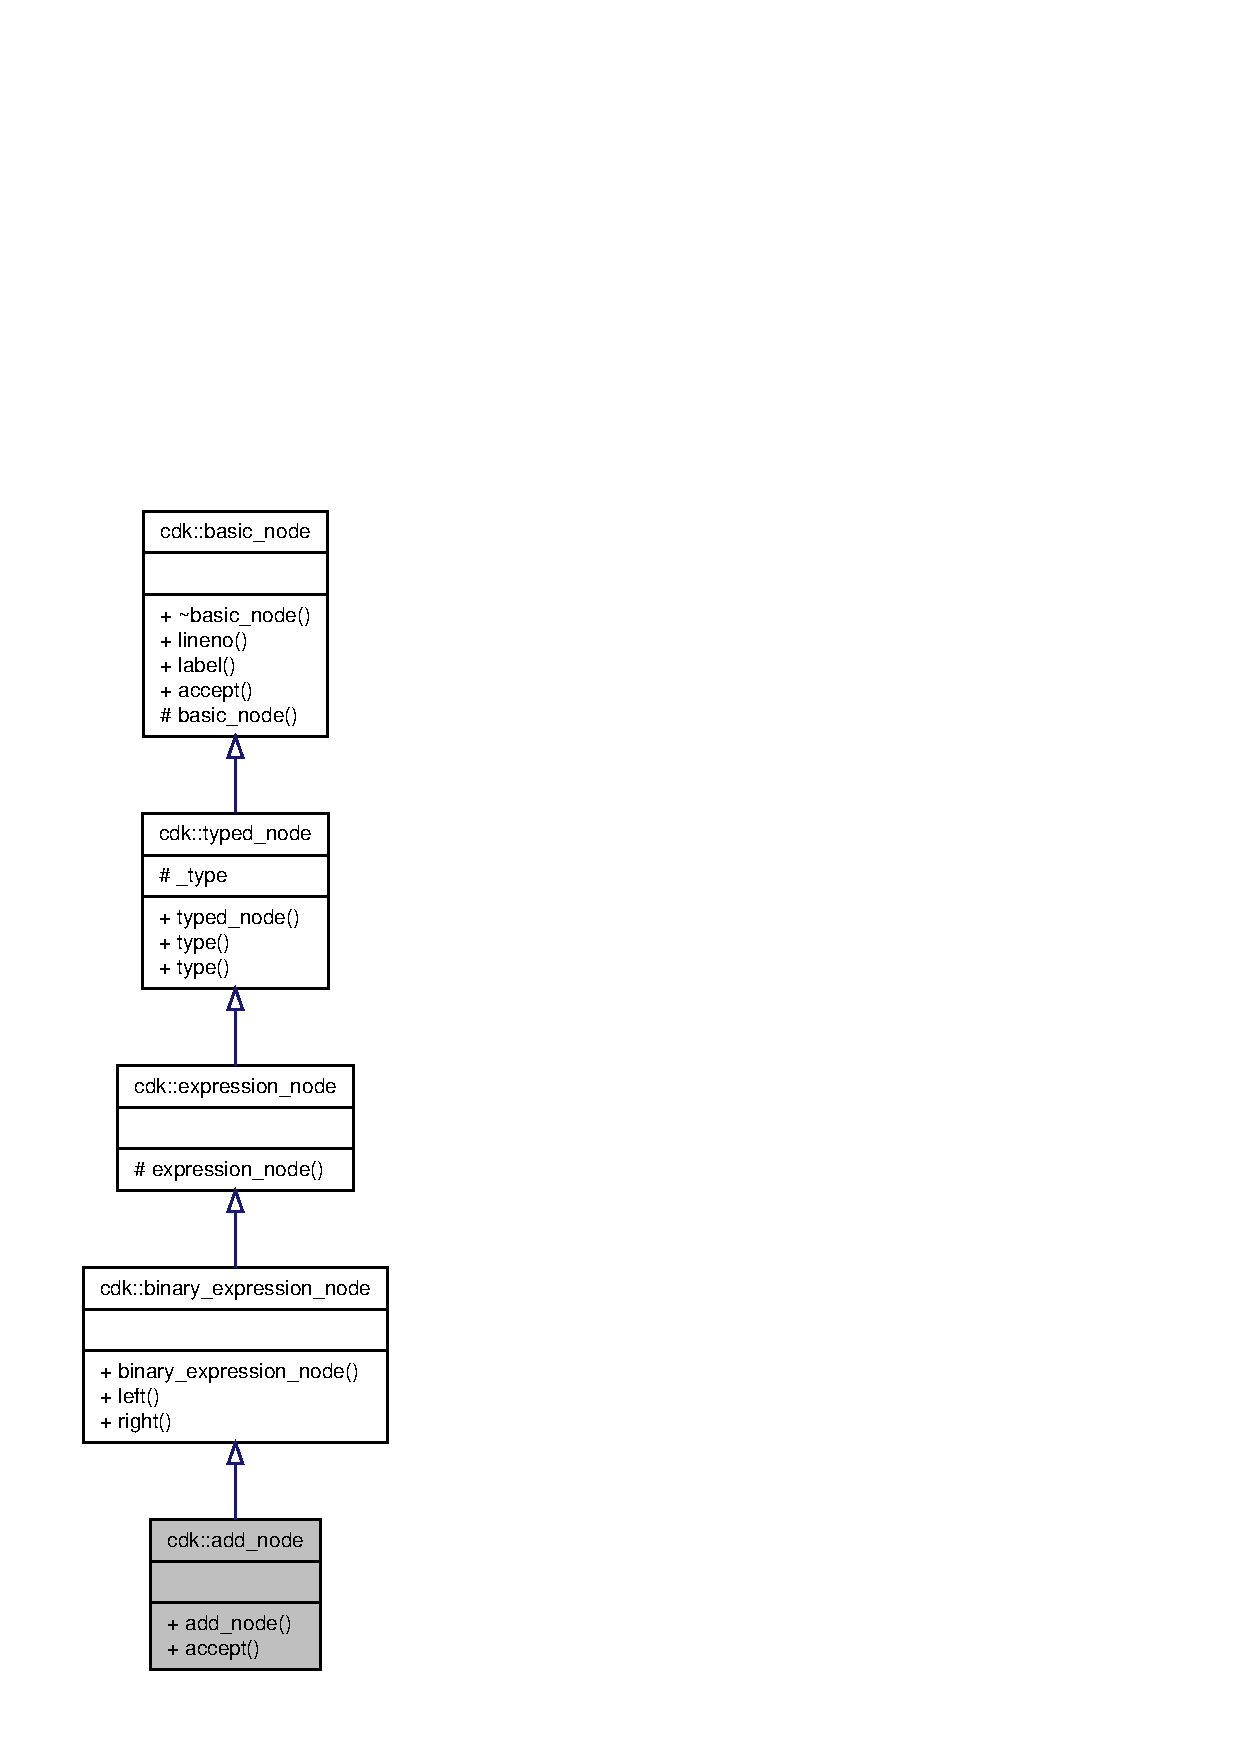
\includegraphics[height=550pt]{classcdk_1_1add__node__inherit__graph}
\end{center}
\end{figure}


Collaboration diagram for cdk\+:\+:add\+\_\+node\+:
\nopagebreak
\begin{figure}[H]
\begin{center}
\leavevmode
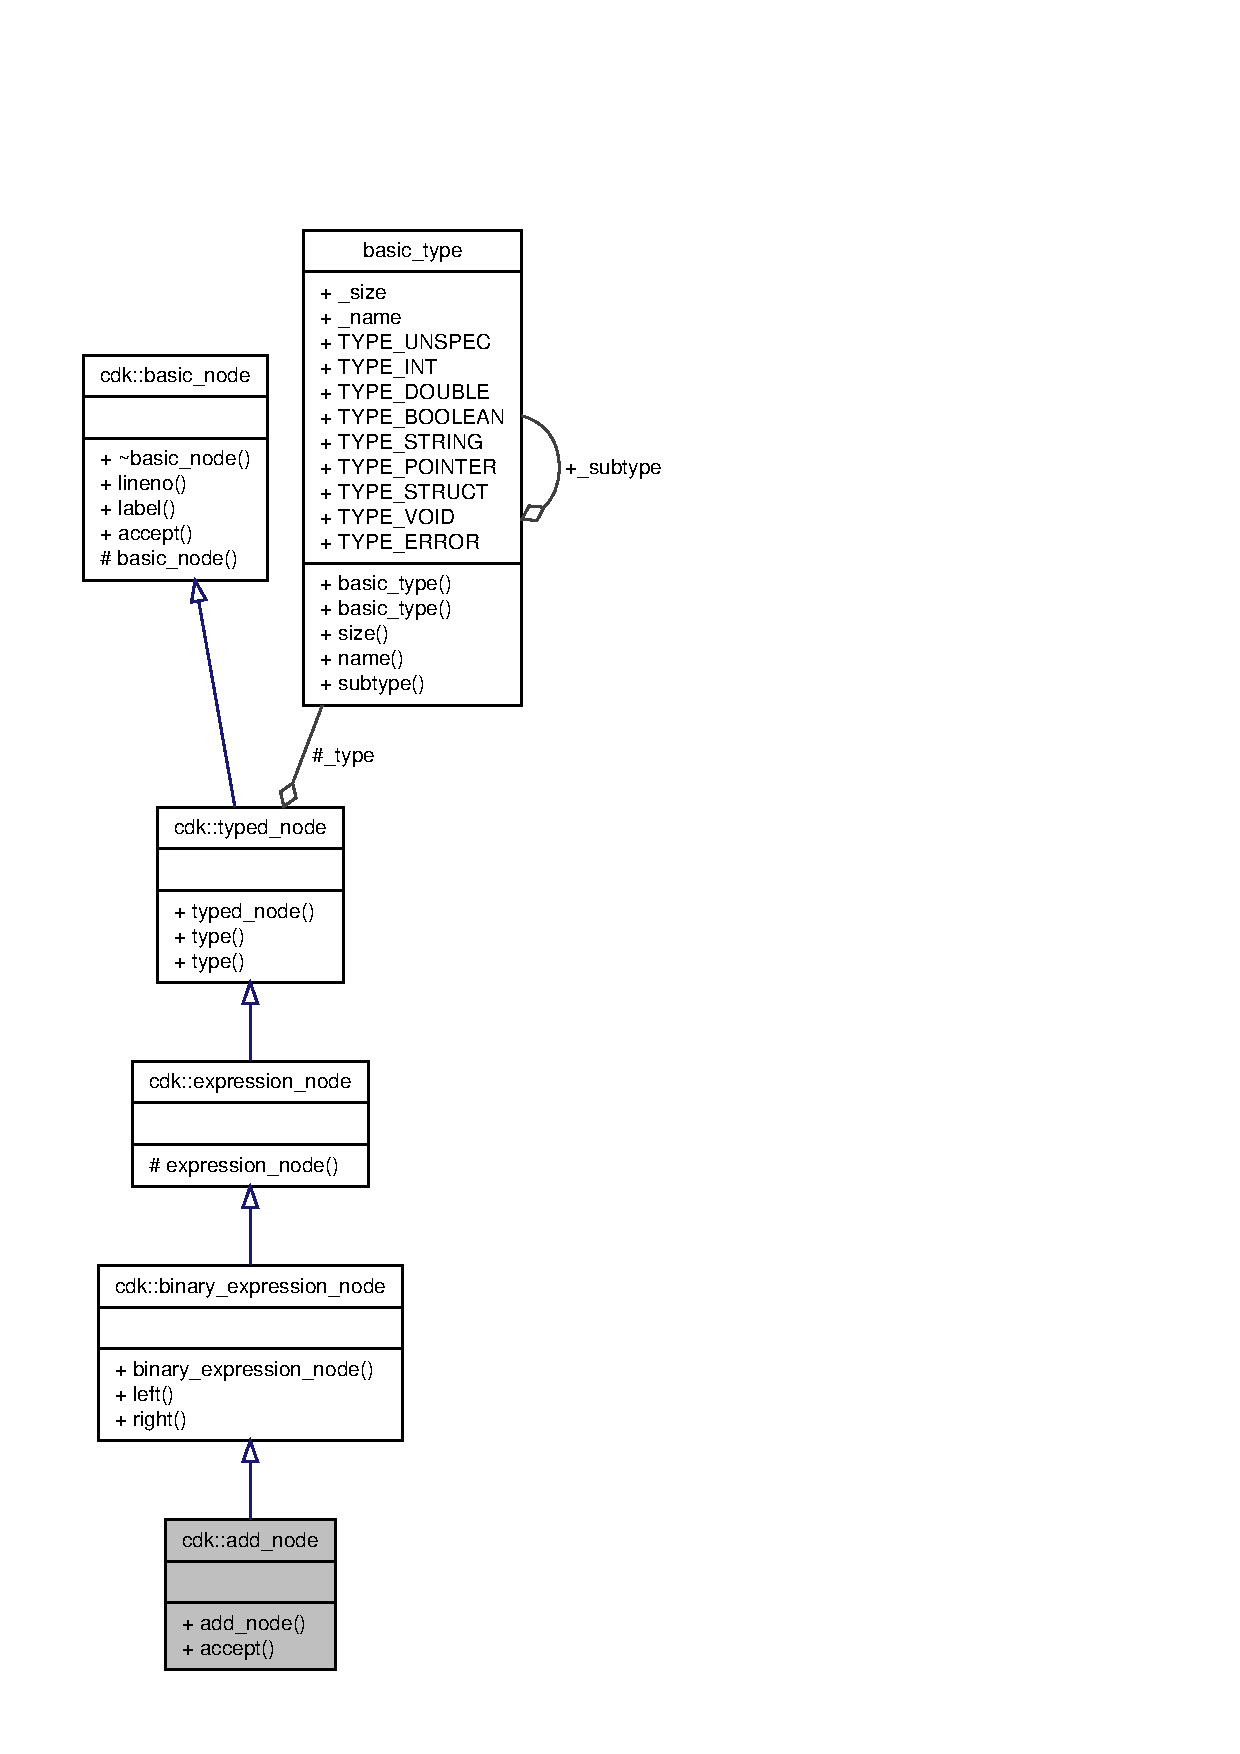
\includegraphics[height=550pt]{classcdk_1_1add__node__coll__graph}
\end{center}
\end{figure}
\subsection*{Public Member Functions}
\begin{DoxyCompactItemize}
\item 
\textbf{ add\+\_\+node} (int \textbf{ lineno}, \textbf{ expression\+\_\+node} $\ast$left, \textbf{ expression\+\_\+node} $\ast$right)
\item 
void \textbf{ accept} (\textbf{ basic\+\_\+ast\+\_\+visitor} $\ast$sp, int level)
\end{DoxyCompactItemize}
\subsection*{Additional Inherited Members}


\subsection{Detailed Description}
Class for describing the addition (\textquotesingle{}+\textquotesingle{}) operator 

Definition at line 11 of file add\+\_\+node.\+h.



\subsection{Constructor \& Destructor Documentation}
\mbox{\label{classcdk_1_1add__node_a560eaccea3678c70d14660f91b4b349f}} 
\index{cdk\+::add\+\_\+node@{cdk\+::add\+\_\+node}!add\+\_\+node@{add\+\_\+node}}
\index{add\+\_\+node@{add\+\_\+node}!cdk\+::add\+\_\+node@{cdk\+::add\+\_\+node}}
\subsubsection{add\+\_\+node()}
{\footnotesize\ttfamily cdk\+::add\+\_\+node\+::add\+\_\+node (\begin{DoxyParamCaption}\item[{int}]{lineno,  }\item[{\textbf{ expression\+\_\+node} $\ast$}]{left,  }\item[{\textbf{ expression\+\_\+node} $\ast$}]{right }\end{DoxyParamCaption})\hspace{0.3cm}{\ttfamily [inline]}}


\begin{DoxyParams}{Parameters}
{\em lineno} & source code line number for this node \\
\hline
{\em left} & first operand \\
\hline
{\em right} & second operand \\
\hline
\end{DoxyParams}


Definition at line 18 of file add\+\_\+node.\+h.



\subsection{Member Function Documentation}
\mbox{\label{classcdk_1_1add__node_a5a0a7fd1aacfcf589233c9b1cdda59d1}} 
\index{cdk\+::add\+\_\+node@{cdk\+::add\+\_\+node}!accept@{accept}}
\index{accept@{accept}!cdk\+::add\+\_\+node@{cdk\+::add\+\_\+node}}
\subsubsection{accept()}
{\footnotesize\ttfamily void cdk\+::add\+\_\+node\+::accept (\begin{DoxyParamCaption}\item[{\textbf{ basic\+\_\+ast\+\_\+visitor} $\ast$}]{sp,  }\item[{int}]{level }\end{DoxyParamCaption})\hspace{0.3cm}{\ttfamily [inline]}, {\ttfamily [virtual]}}


\begin{DoxyParams}{Parameters}
{\em sp} & semantic processor visitor \\
\hline
{\em level} & syntactic tree level \\
\hline
\end{DoxyParams}


Implements \textbf{ cdk\+::basic\+\_\+node} \doxyref{}{p.}{classcdk_1_1basic__node_ab38adcbc95c46b809961278afae3bf05}.



Definition at line 26 of file add\+\_\+node.\+h.



The documentation for this class was generated from the following file\+:\begin{DoxyCompactItemize}
\item 
ast/add\+\_\+node.\+h\end{DoxyCompactItemize}

\section{cdk\+:\+:and\+\_\+node Class Reference}
\label{classcdk_1_1and__node}\index{cdk\+::and\+\_\+node@{cdk\+::and\+\_\+node}}


{\ttfamily \#include $<$and\+\_\+node.\+h$>$}



Inheritance diagram for cdk\+:\+:and\+\_\+node\+:
\nopagebreak
\begin{figure}[H]
\begin{center}
\leavevmode
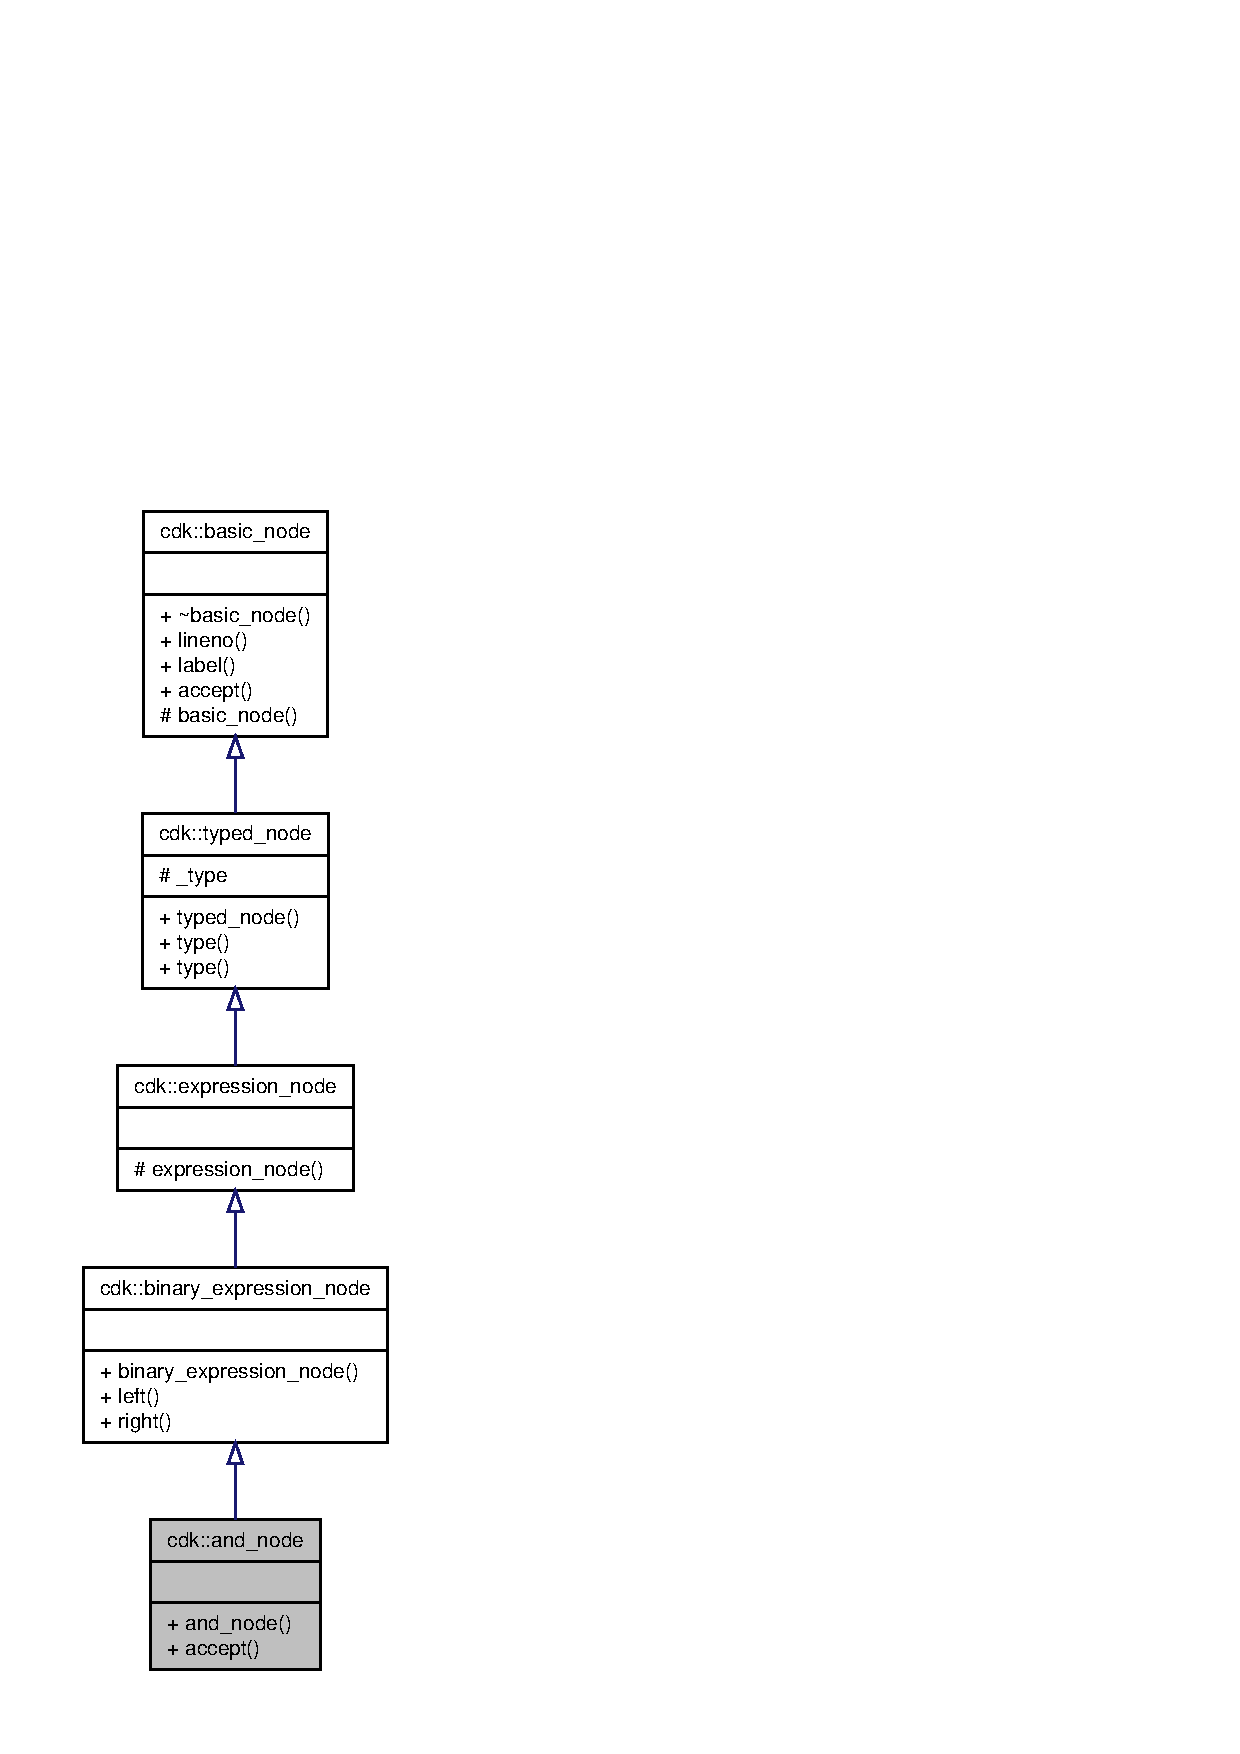
\includegraphics[height=550pt]{classcdk_1_1and__node__inherit__graph}
\end{center}
\end{figure}


Collaboration diagram for cdk\+:\+:and\+\_\+node\+:
\nopagebreak
\begin{figure}[H]
\begin{center}
\leavevmode
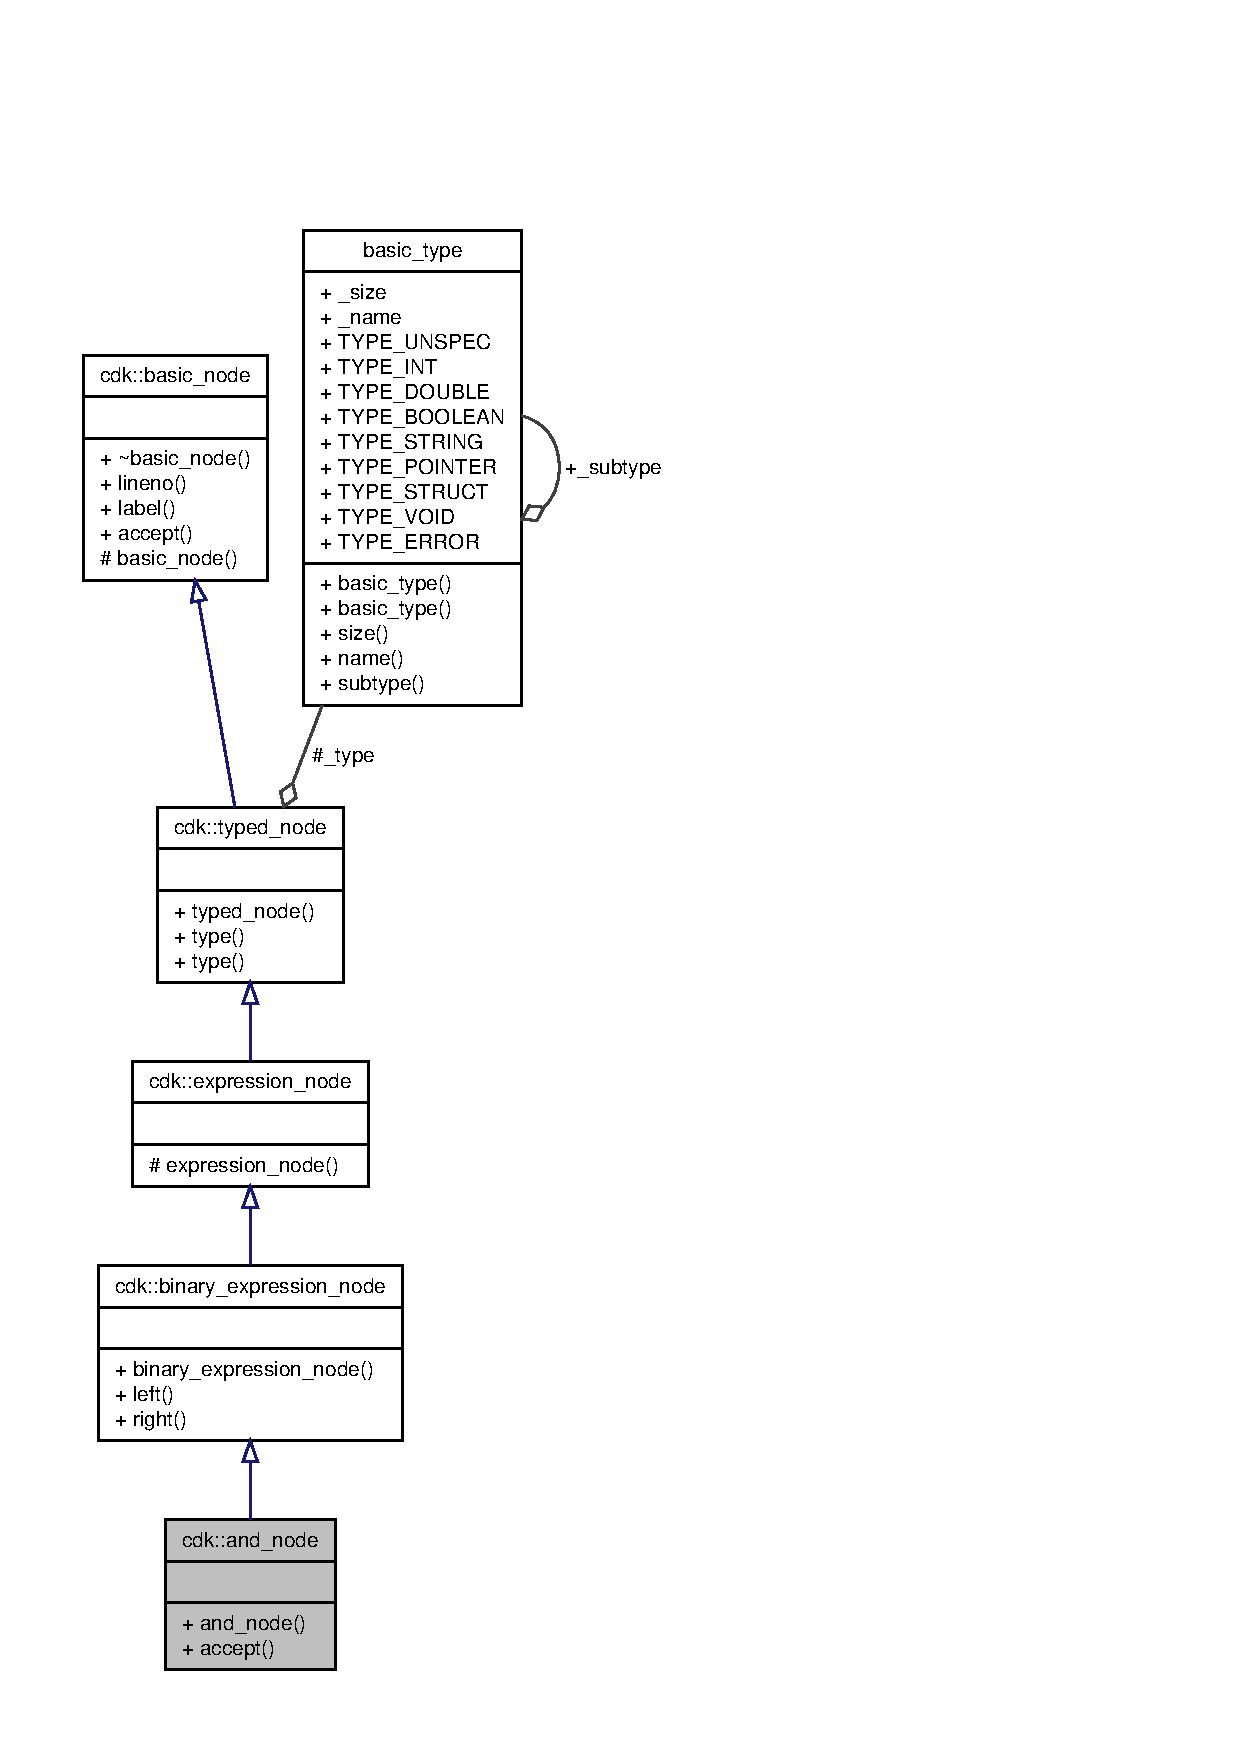
\includegraphics[height=550pt]{classcdk_1_1and__node__coll__graph}
\end{center}
\end{figure}
\subsection*{Public Member Functions}
\begin{DoxyCompactItemize}
\item 
\textbf{ and\+\_\+node} (int \textbf{ lineno}, \textbf{ expression\+\_\+node} $\ast$left, \textbf{ expression\+\_\+node} $\ast$right)
\item 
void \textbf{ accept} (\textbf{ basic\+\_\+ast\+\_\+visitor} $\ast$sp, int level)
\end{DoxyCompactItemize}
\subsection*{Additional Inherited Members}


\subsection{Detailed Description}
Class for describing the and operator 

Definition at line 11 of file and\+\_\+node.\+h.



\subsection{Constructor \& Destructor Documentation}
\mbox{\label{classcdk_1_1and__node_afa47935e1bc2471b65254cb0ab5af17c}} 
\index{cdk\+::and\+\_\+node@{cdk\+::and\+\_\+node}!and\+\_\+node@{and\+\_\+node}}
\index{and\+\_\+node@{and\+\_\+node}!cdk\+::and\+\_\+node@{cdk\+::and\+\_\+node}}
\subsubsection{and\+\_\+node()}
{\footnotesize\ttfamily cdk\+::and\+\_\+node\+::and\+\_\+node (\begin{DoxyParamCaption}\item[{int}]{lineno,  }\item[{\textbf{ expression\+\_\+node} $\ast$}]{left,  }\item[{\textbf{ expression\+\_\+node} $\ast$}]{right }\end{DoxyParamCaption})\hspace{0.3cm}{\ttfamily [inline]}}


\begin{DoxyParams}{Parameters}
{\em lineno} & source code line number for this node \\
\hline
{\em left} & first operand \\
\hline
{\em right} & second operand \\
\hline
\end{DoxyParams}


Definition at line 19 of file and\+\_\+node.\+h.



\subsection{Member Function Documentation}
\mbox{\label{classcdk_1_1and__node_a6bfbb0fa5db8f100c88b196c791135d7}} 
\index{cdk\+::and\+\_\+node@{cdk\+::and\+\_\+node}!accept@{accept}}
\index{accept@{accept}!cdk\+::and\+\_\+node@{cdk\+::and\+\_\+node}}
\subsubsection{accept()}
{\footnotesize\ttfamily void cdk\+::and\+\_\+node\+::accept (\begin{DoxyParamCaption}\item[{\textbf{ basic\+\_\+ast\+\_\+visitor} $\ast$}]{sp,  }\item[{int}]{level }\end{DoxyParamCaption})\hspace{0.3cm}{\ttfamily [inline]}, {\ttfamily [virtual]}}


\begin{DoxyParams}{Parameters}
{\em sp} & semantic processor visitor \\
\hline
{\em level} & syntactic tree level \\
\hline
\end{DoxyParams}


Implements \textbf{ cdk\+::basic\+\_\+node} \doxyref{}{p.}{classcdk_1_1basic__node_ab38adcbc95c46b809961278afae3bf05}.



Definition at line 27 of file and\+\_\+node.\+h.



The documentation for this class was generated from the following file\+:\begin{DoxyCompactItemize}
\item 
ast/and\+\_\+node.\+h\end{DoxyCompactItemize}

\section{cdk\+:\+:assignment\+\_\+node Class Reference}
\label{classcdk_1_1assignment__node}\index{cdk\+::assignment\+\_\+node@{cdk\+::assignment\+\_\+node}}


{\ttfamily \#include $<$assignment\+\_\+node.\+h$>$}



Inheritance diagram for cdk\+:\+:assignment\+\_\+node\+:
\nopagebreak
\begin{figure}[H]
\begin{center}
\leavevmode
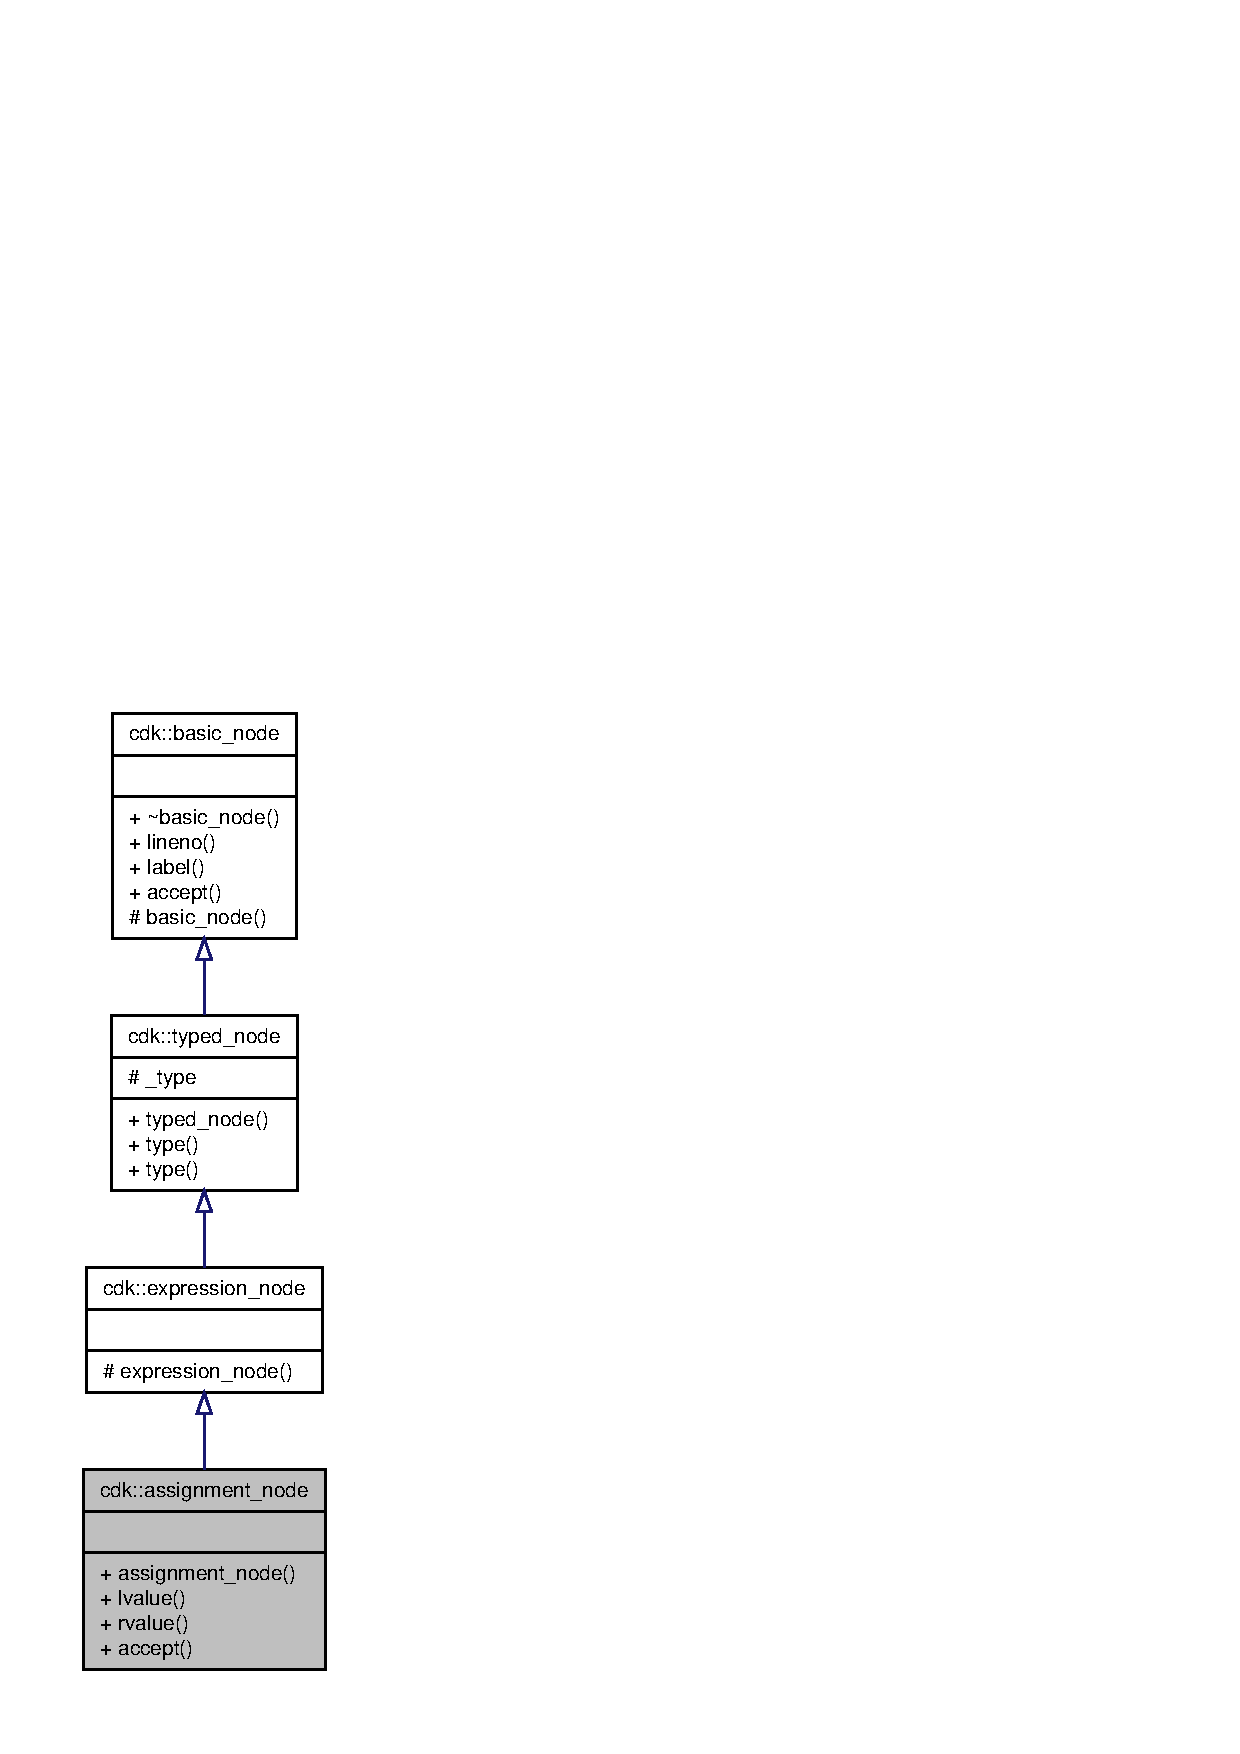
\includegraphics[width=160pt]{classcdk_1_1assignment__node__inherit__graph}
\end{center}
\end{figure}


Collaboration diagram for cdk\+:\+:assignment\+\_\+node\+:
\nopagebreak
\begin{figure}[H]
\begin{center}
\leavevmode
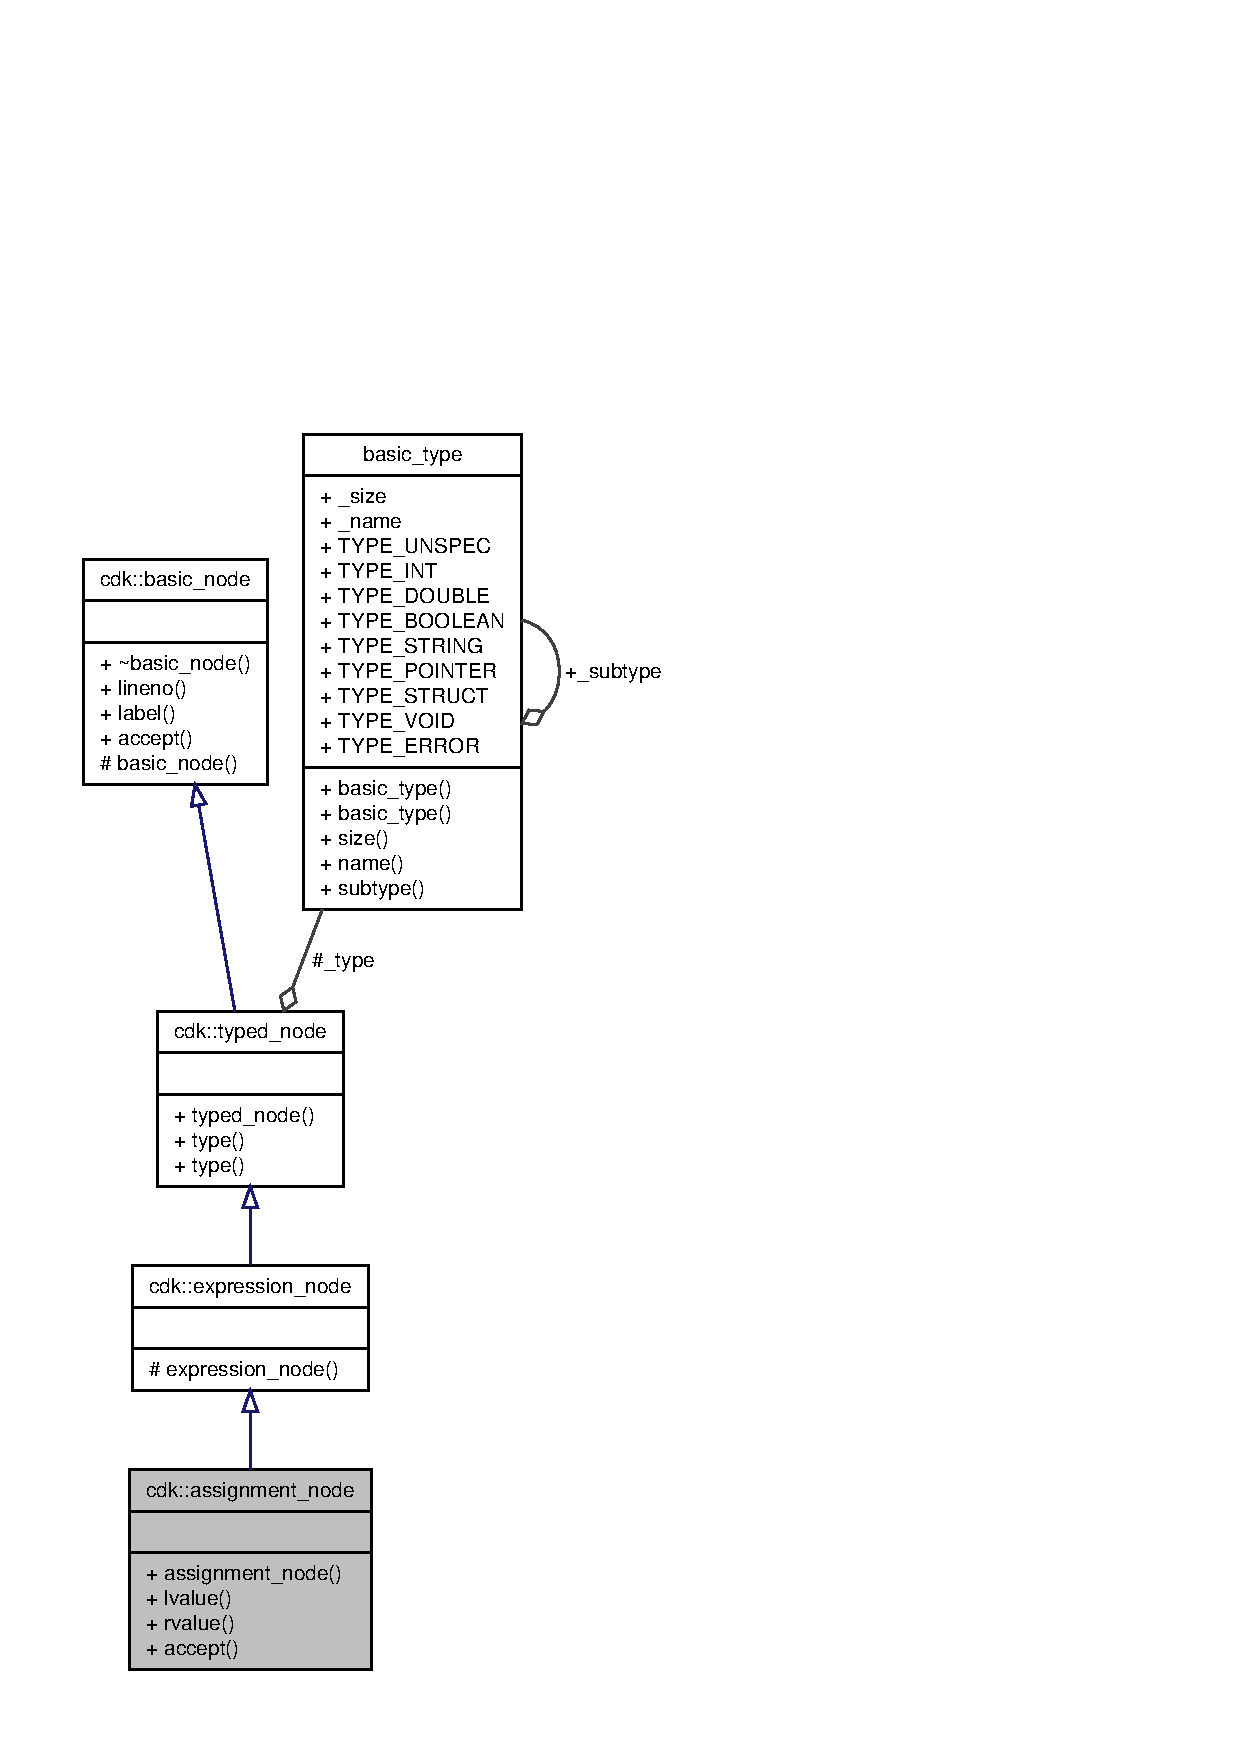
\includegraphics[height=550pt]{classcdk_1_1assignment__node__coll__graph}
\end{center}
\end{figure}
\subsection*{Public Member Functions}
\begin{DoxyCompactItemize}
\item 
\mbox{\label{classcdk_1_1assignment__node_a644ee5157596c9aaa29007d6e72a4844}} 
{\bfseries assignment\+\_\+node} (int \textbf{ lineno}, \textbf{ lvalue\+\_\+node} $\ast$lvalue, \textbf{ expression\+\_\+node} $\ast$rvalue)
\item 
\mbox{\label{classcdk_1_1assignment__node_af31fd118676196fe9619793ba4c9e237}} 
\textbf{ lvalue\+\_\+node} $\ast$ {\bfseries lvalue} ()
\item 
\mbox{\label{classcdk_1_1assignment__node_a997b389454803f72566a2d77590859a5}} 
\textbf{ expression\+\_\+node} $\ast$ {\bfseries rvalue} ()
\item 
void \textbf{ accept} (\textbf{ basic\+\_\+ast\+\_\+visitor} $\ast$sp, int level)
\end{DoxyCompactItemize}
\subsection*{Additional Inherited Members}


\subsection{Detailed Description}
Class for describing assignment nodes. 

Definition at line 12 of file assignment\+\_\+node.\+h.



\subsection{Member Function Documentation}
\mbox{\label{classcdk_1_1assignment__node_a02ccd8c51da2f61195e994db3f482c4f}} 
\index{cdk\+::assignment\+\_\+node@{cdk\+::assignment\+\_\+node}!accept@{accept}}
\index{accept@{accept}!cdk\+::assignment\+\_\+node@{cdk\+::assignment\+\_\+node}}
\subsubsection{accept()}
{\footnotesize\ttfamily void cdk\+::assignment\+\_\+node\+::accept (\begin{DoxyParamCaption}\item[{\textbf{ basic\+\_\+ast\+\_\+visitor} $\ast$}]{sp,  }\item[{int}]{level }\end{DoxyParamCaption})\hspace{0.3cm}{\ttfamily [inline]}, {\ttfamily [virtual]}}

Every node must provide this method.


\begin{DoxyParams}{Parameters}
{\em sp} & semantic processor visitor \\
\hline
{\em level} & syntactic tree level \\
\hline
\end{DoxyParams}


Implements \textbf{ cdk\+::basic\+\_\+node} \doxyref{}{p.}{classcdk_1_1basic__node_ab38adcbc95c46b809961278afae3bf05}.



Definition at line 29 of file assignment\+\_\+node.\+h.



The documentation for this class was generated from the following file\+:\begin{DoxyCompactItemize}
\item 
ast/assignment\+\_\+node.\+h\end{DoxyCompactItemize}

\section{basic\+\_\+ast\+\_\+visitor Class Reference}
\label{classbasic__ast__visitor}\index{basic\+\_\+ast\+\_\+visitor@{basic\+\_\+ast\+\_\+visitor}}


{\ttfamily \#include $<$basic\+\_\+ast\+\_\+visitor.\+h$>$}



Collaboration diagram for basic\+\_\+ast\+\_\+visitor\+:
\nopagebreak
\begin{figure}[H]
\begin{center}
\leavevmode
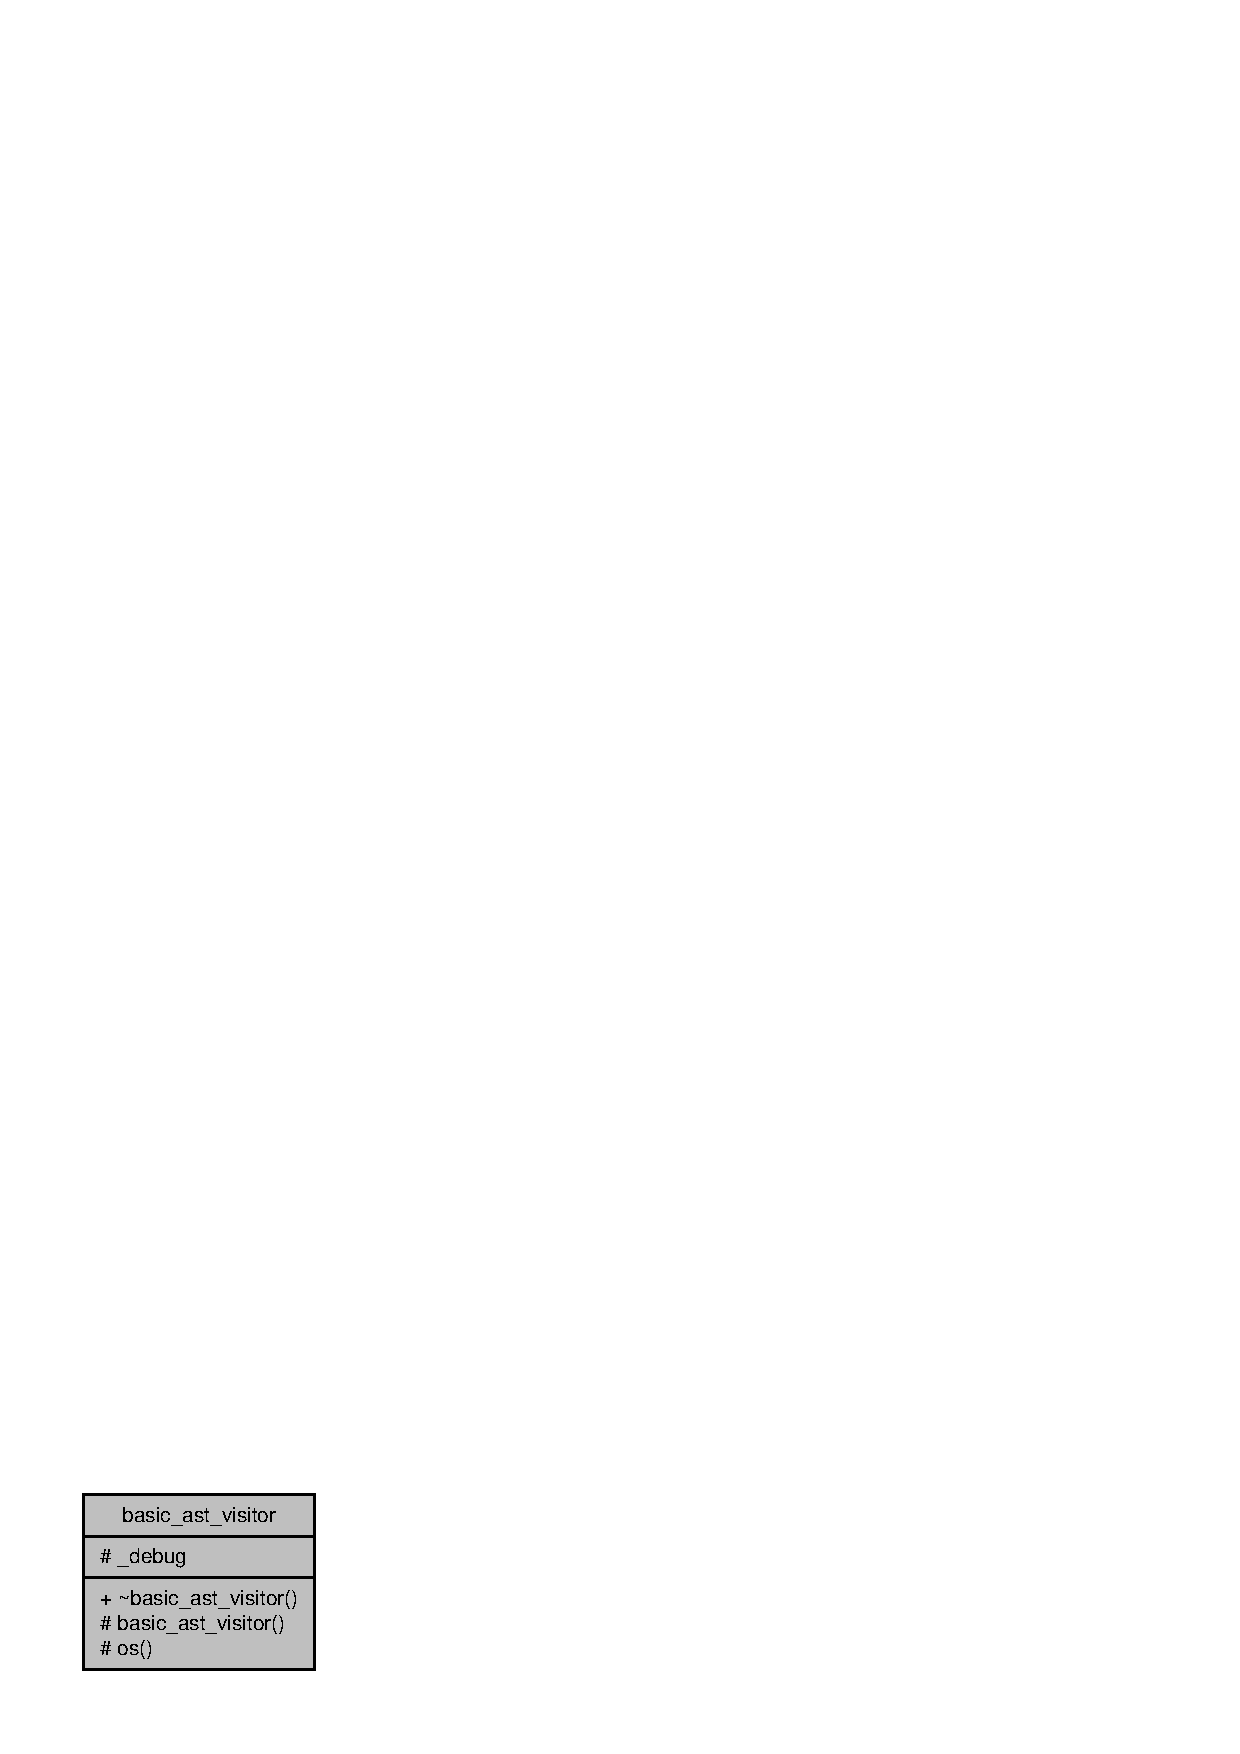
\includegraphics[width=155pt]{classbasic__ast__visitor__coll__graph}
\end{center}
\end{figure}
\subsection*{Public Member Functions}
\begin{DoxyCompactItemize}
\item 
virtual \textbf{ $\sim$basic\+\_\+ast\+\_\+visitor} ()
\end{DoxyCompactItemize}
\subsection*{Protected Member Functions}
\begin{DoxyCompactItemize}
\item 
\textbf{ basic\+\_\+ast\+\_\+visitor} (std\+::ostream \&\textbf{ os}=std\+::cout, bool debug=false)
\item 
std\+::ostream \& \textbf{ os} ()
\end{DoxyCompactItemize}
\subsection*{Protected Attributes}
\begin{DoxyCompactItemize}
\item 
\mbox{\label{classbasic__ast__visitor_a00d9f815e553a3313b33a952e03702f4}} 
bool \textbf{ \+\_\+debug}
\begin{DoxyCompactList}\small\item\em Debug flag. \end{DoxyCompactList}\end{DoxyCompactItemize}


\subsection{Detailed Description}
This class is only for compiling the package\+: it will not be installed. Specific compilers are supposed to define their own, with the S\+A\+ME N\+A\+ME, but defining A\+LL processing functions corresponding to their specific problem. 

Definition at line 17 of file basic\+\_\+ast\+\_\+visitor.\+h.



\subsection{Constructor \& Destructor Documentation}
\mbox{\label{classbasic__ast__visitor_a194d2f7cced321e384b68782d8e33a47}} 
\index{basic\+\_\+ast\+\_\+visitor@{basic\+\_\+ast\+\_\+visitor}!basic\+\_\+ast\+\_\+visitor@{basic\+\_\+ast\+\_\+visitor}}
\index{basic\+\_\+ast\+\_\+visitor@{basic\+\_\+ast\+\_\+visitor}!basic\+\_\+ast\+\_\+visitor@{basic\+\_\+ast\+\_\+visitor}}
\subsubsection{basic\+\_\+ast\+\_\+visitor()}
{\footnotesize\ttfamily basic\+\_\+ast\+\_\+visitor\+::basic\+\_\+ast\+\_\+visitor (\begin{DoxyParamCaption}\item[{std\+::ostream \&}]{os = {\ttfamily std\+:\+:cout},  }\item[{bool}]{debug = {\ttfamily false} }\end{DoxyParamCaption})\hspace{0.3cm}{\ttfamily [protected]}}

Initialization of a semantic processor.


\begin{DoxyParams}{Parameters}
{\em os} & is the output stream to be used by the semantic processor. \\
\hline
\end{DoxyParams}
\mbox{\label{classbasic__ast__visitor_a110508f9dd86fc1472ffee3d2b3bd0f5}} 
\index{basic\+\_\+ast\+\_\+visitor@{basic\+\_\+ast\+\_\+visitor}!````~basic\+\_\+ast\+\_\+visitor@{$\sim$basic\+\_\+ast\+\_\+visitor}}
\index{````~basic\+\_\+ast\+\_\+visitor@{$\sim$basic\+\_\+ast\+\_\+visitor}!basic\+\_\+ast\+\_\+visitor@{basic\+\_\+ast\+\_\+visitor}}
\subsubsection{$\sim$basic\+\_\+ast\+\_\+visitor()}
{\footnotesize\ttfamily virtual basic\+\_\+ast\+\_\+visitor\+::$\sim$basic\+\_\+ast\+\_\+visitor (\begin{DoxyParamCaption}{ }\end{DoxyParamCaption})\hspace{0.3cm}{\ttfamily [virtual]}}

How to destroy a semantic processor. 

\subsection{Member Function Documentation}
\mbox{\label{classbasic__ast__visitor_ab81ab147fe687470c3e8f9ebfd2ca6f9}} 
\index{basic\+\_\+ast\+\_\+visitor@{basic\+\_\+ast\+\_\+visitor}!os@{os}}
\index{os@{os}!basic\+\_\+ast\+\_\+visitor@{basic\+\_\+ast\+\_\+visitor}}
\subsubsection{os()}
{\footnotesize\ttfamily std\+::ostream\& basic\+\_\+ast\+\_\+visitor\+::os (\begin{DoxyParamCaption}{ }\end{DoxyParamCaption})\hspace{0.3cm}{\ttfamily [inline]}, {\ttfamily [protected]}}

Return the current output stream. \begin{DoxyReturn}{Returns}
an output stream. 
\end{DoxyReturn}


Definition at line 38 of file basic\+\_\+ast\+\_\+visitor.\+h.



The documentation for this class was generated from the following file\+:\begin{DoxyCompactItemize}
\item 
basic\+\_\+ast\+\_\+visitor.\+h\end{DoxyCompactItemize}

\section{cdk\+:\+:basic\+\_\+factory Class Reference}
\label{classcdk_1_1basic__factory}\index{cdk\+::basic\+\_\+factory@{cdk\+::basic\+\_\+factory}}


{\ttfamily \#include $<$basic\+\_\+factory.\+h$>$}



Inheritance diagram for cdk\+:\+:basic\+\_\+factory\+:
\nopagebreak
\begin{figure}[H]
\begin{center}
\leavevmode
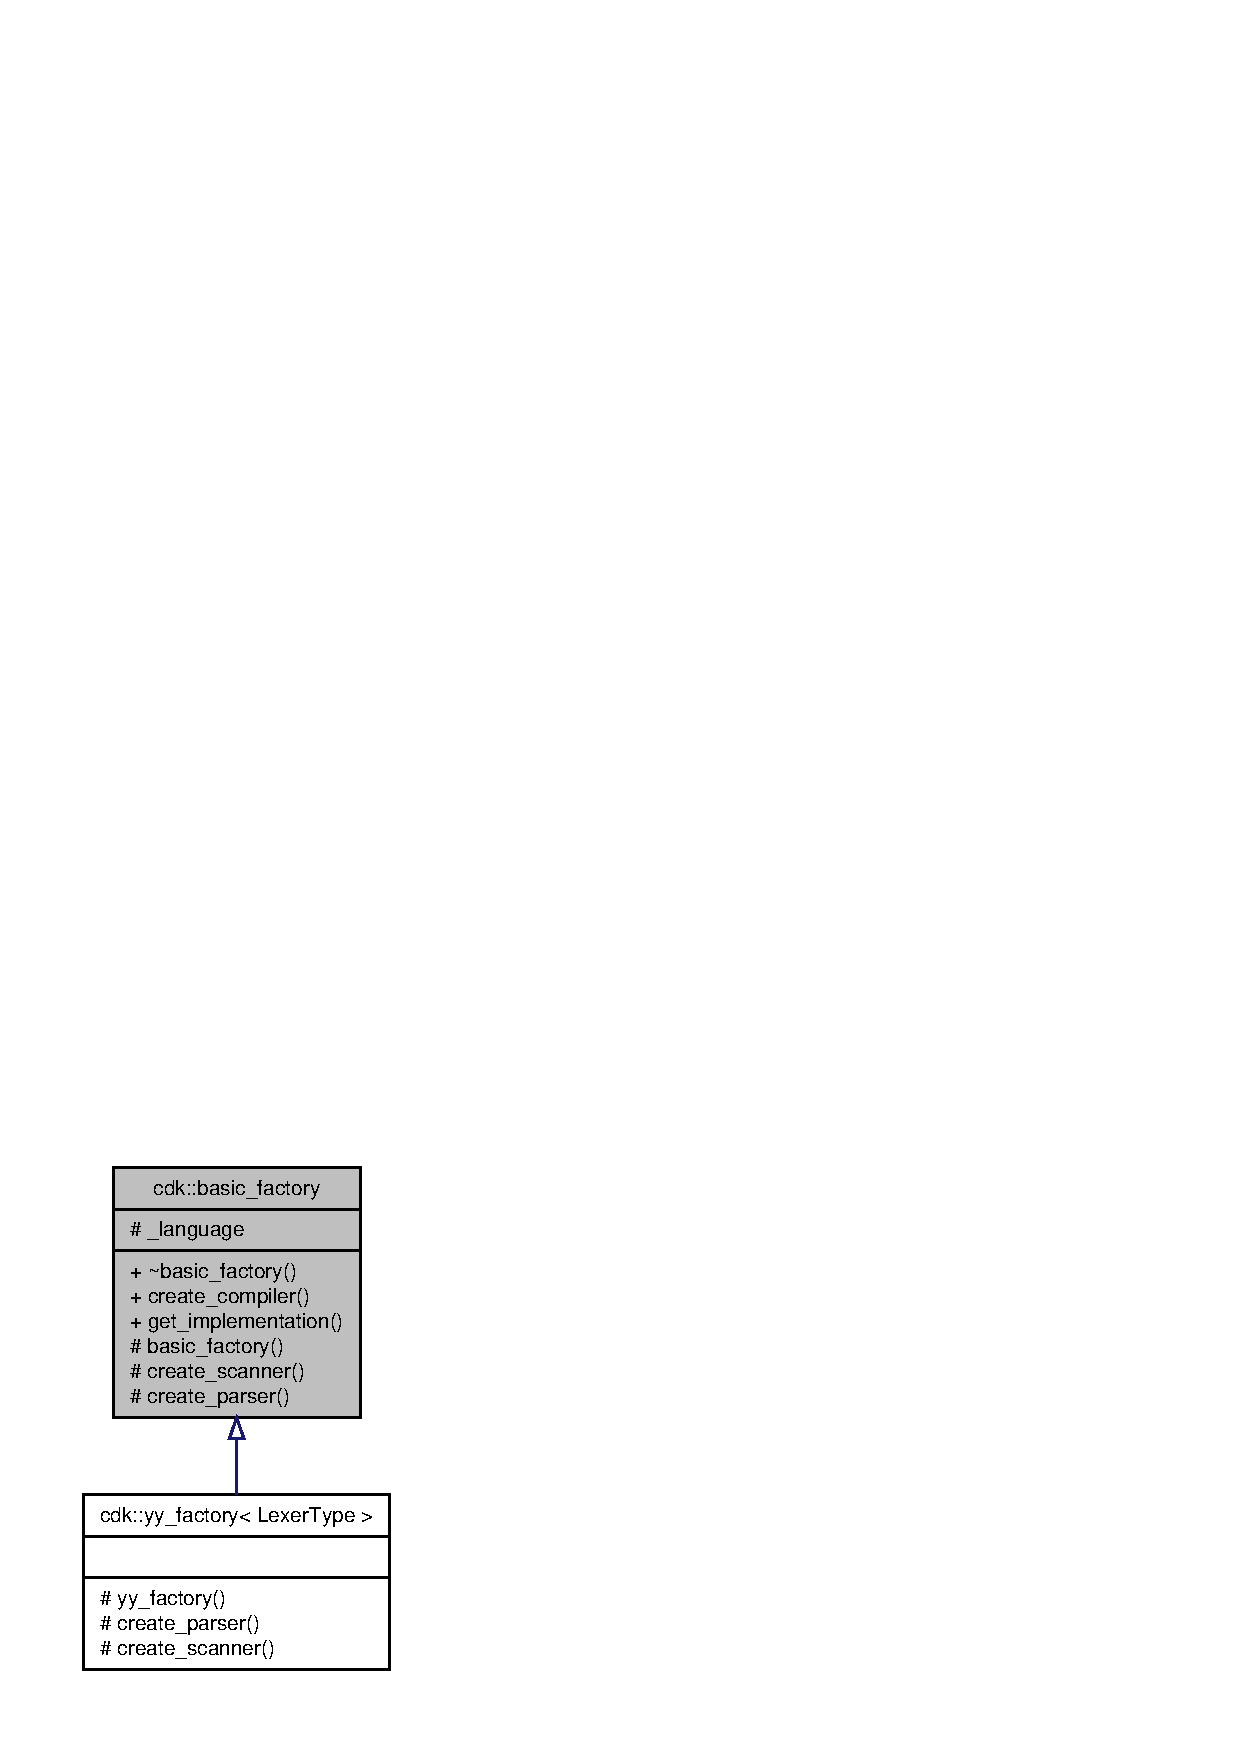
\includegraphics[width=191pt]{classcdk_1_1basic__factory__inherit__graph}
\end{center}
\end{figure}


Collaboration diagram for cdk\+:\+:basic\+\_\+factory\+:
\nopagebreak
\begin{figure}[H]
\begin{center}
\leavevmode
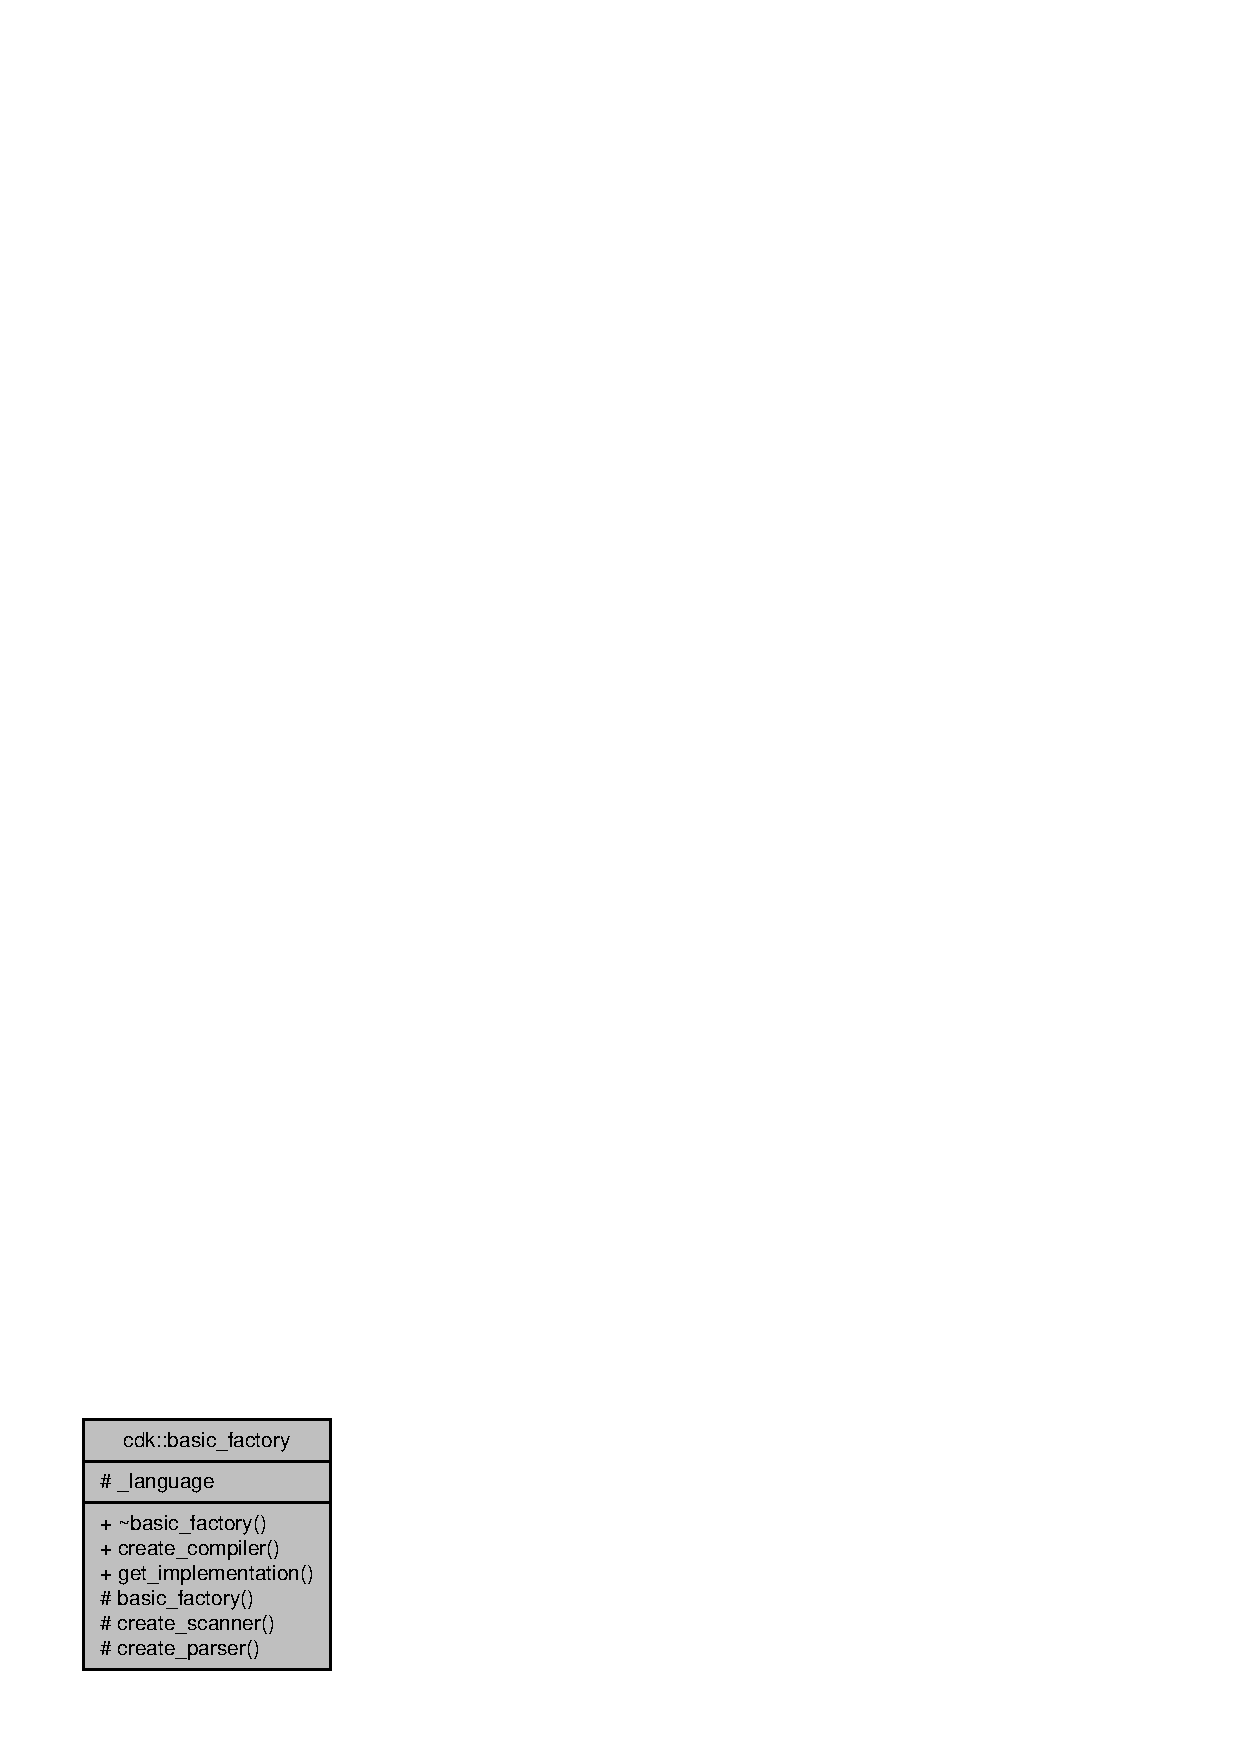
\includegraphics[width=163pt]{classcdk_1_1basic__factory__coll__graph}
\end{center}
\end{figure}
\subsection*{Public Member Functions}
\begin{DoxyCompactItemize}
\item 
virtual \textbf{ $\sim$basic\+\_\+factory} ()
\item 
virtual std\+::shared\+\_\+ptr$<$ \textbf{ compiler} $>$ \textbf{ create\+\_\+compiler} ()
\end{DoxyCompactItemize}
\subsection*{Static Public Member Functions}
\begin{DoxyCompactItemize}
\item 
\mbox{\label{classcdk_1_1basic__factory_a535fded0c301dc7d002f17fe631d5fa9}} 
static \textbf{ basic\+\_\+factory} $\ast$ {\bfseries get\+\_\+implementation} (const std\+::string \&language)
\end{DoxyCompactItemize}
\subsection*{Protected Member Functions}
\begin{DoxyCompactItemize}
\item 
\mbox{\label{classcdk_1_1basic__factory_ad6019ad813cd6a082284cd4265d2ea5a}} 
{\bfseries basic\+\_\+factory} (const std\+::string \&language)
\item 
virtual std\+::shared\+\_\+ptr$<$ \textbf{ basic\+\_\+scanner} $>$ \textbf{ create\+\_\+scanner} ()=0
\item 
virtual std\+::shared\+\_\+ptr$<$ \textbf{ basic\+\_\+parser} $>$ \textbf{ create\+\_\+parser} ()=0
\end{DoxyCompactItemize}
\subsection*{Protected Attributes}
\begin{DoxyCompactItemize}
\item 
\mbox{\label{classcdk_1_1basic__factory_a8c4a1162265812837a9a001973cc9a3a}} 
const std\+::string {\bfseries \+\_\+language} = \char`\"{}\char`\"{}
\end{DoxyCompactItemize}


\subsection{Detailed Description}
This is the main factory abstract class\+: it provides methods for creating the lexical analyser and the compiler itself. Instances of concrete subclasses will be created by the \char`\"{}main\char`\"{} function to provide instances of the scanner and compiler objects for a concrete language.
\begin{DoxyItemize}
\item keys are language names
\item values are compiler factories 
\end{DoxyItemize}

Definition at line 24 of file basic\+\_\+factory.\+h.



\subsection{Constructor \& Destructor Documentation}
\mbox{\label{classcdk_1_1basic__factory_a9cb78539bfef6fef3429337c42b78554}} 
\index{cdk\+::basic\+\_\+factory@{cdk\+::basic\+\_\+factory}!````~basic\+\_\+factory@{$\sim$basic\+\_\+factory}}
\index{````~basic\+\_\+factory@{$\sim$basic\+\_\+factory}!cdk\+::basic\+\_\+factory@{cdk\+::basic\+\_\+factory}}
\subsubsection{$\sim$basic\+\_\+factory()}
{\footnotesize\ttfamily virtual cdk\+::basic\+\_\+factory\+::$\sim$basic\+\_\+factory (\begin{DoxyParamCaption}{ }\end{DoxyParamCaption})\hspace{0.3cm}{\ttfamily [inline]}, {\ttfamily [virtual]}}

The superclass destructor does not do anything. Probably, it would be a good idea to clean up the factories map. 

Definition at line 52 of file basic\+\_\+factory.\+h.



\subsection{Member Function Documentation}
\mbox{\label{classcdk_1_1basic__factory_a883cf0f3e52b5a53b316914c74535de7}} 
\index{cdk\+::basic\+\_\+factory@{cdk\+::basic\+\_\+factory}!create\+\_\+compiler@{create\+\_\+compiler}}
\index{create\+\_\+compiler@{create\+\_\+compiler}!cdk\+::basic\+\_\+factory@{cdk\+::basic\+\_\+factory}}
\subsubsection{create\+\_\+compiler()}
{\footnotesize\ttfamily virtual std\+::shared\+\_\+ptr$<$\textbf{ compiler}$>$ cdk\+::basic\+\_\+factory\+::create\+\_\+compiler (\begin{DoxyParamCaption}{ }\end{DoxyParamCaption})\hspace{0.3cm}{\ttfamily [inline]}, {\ttfamily [virtual]}}

Create a compiler object for a given language. 
\begin{DoxyParams}{Parameters}
{\em name} & name of the language handled by the compiler \\
\hline
\end{DoxyParams}
\begin{DoxyReturn}{Returns}
compiler object pointer 
\end{DoxyReturn}


Definition at line 78 of file basic\+\_\+factory.\+h.



References create\+\_\+parser(), and create\+\_\+scanner().

Here is the call graph for this function\+:
\nopagebreak
\begin{figure}[H]
\begin{center}
\leavevmode
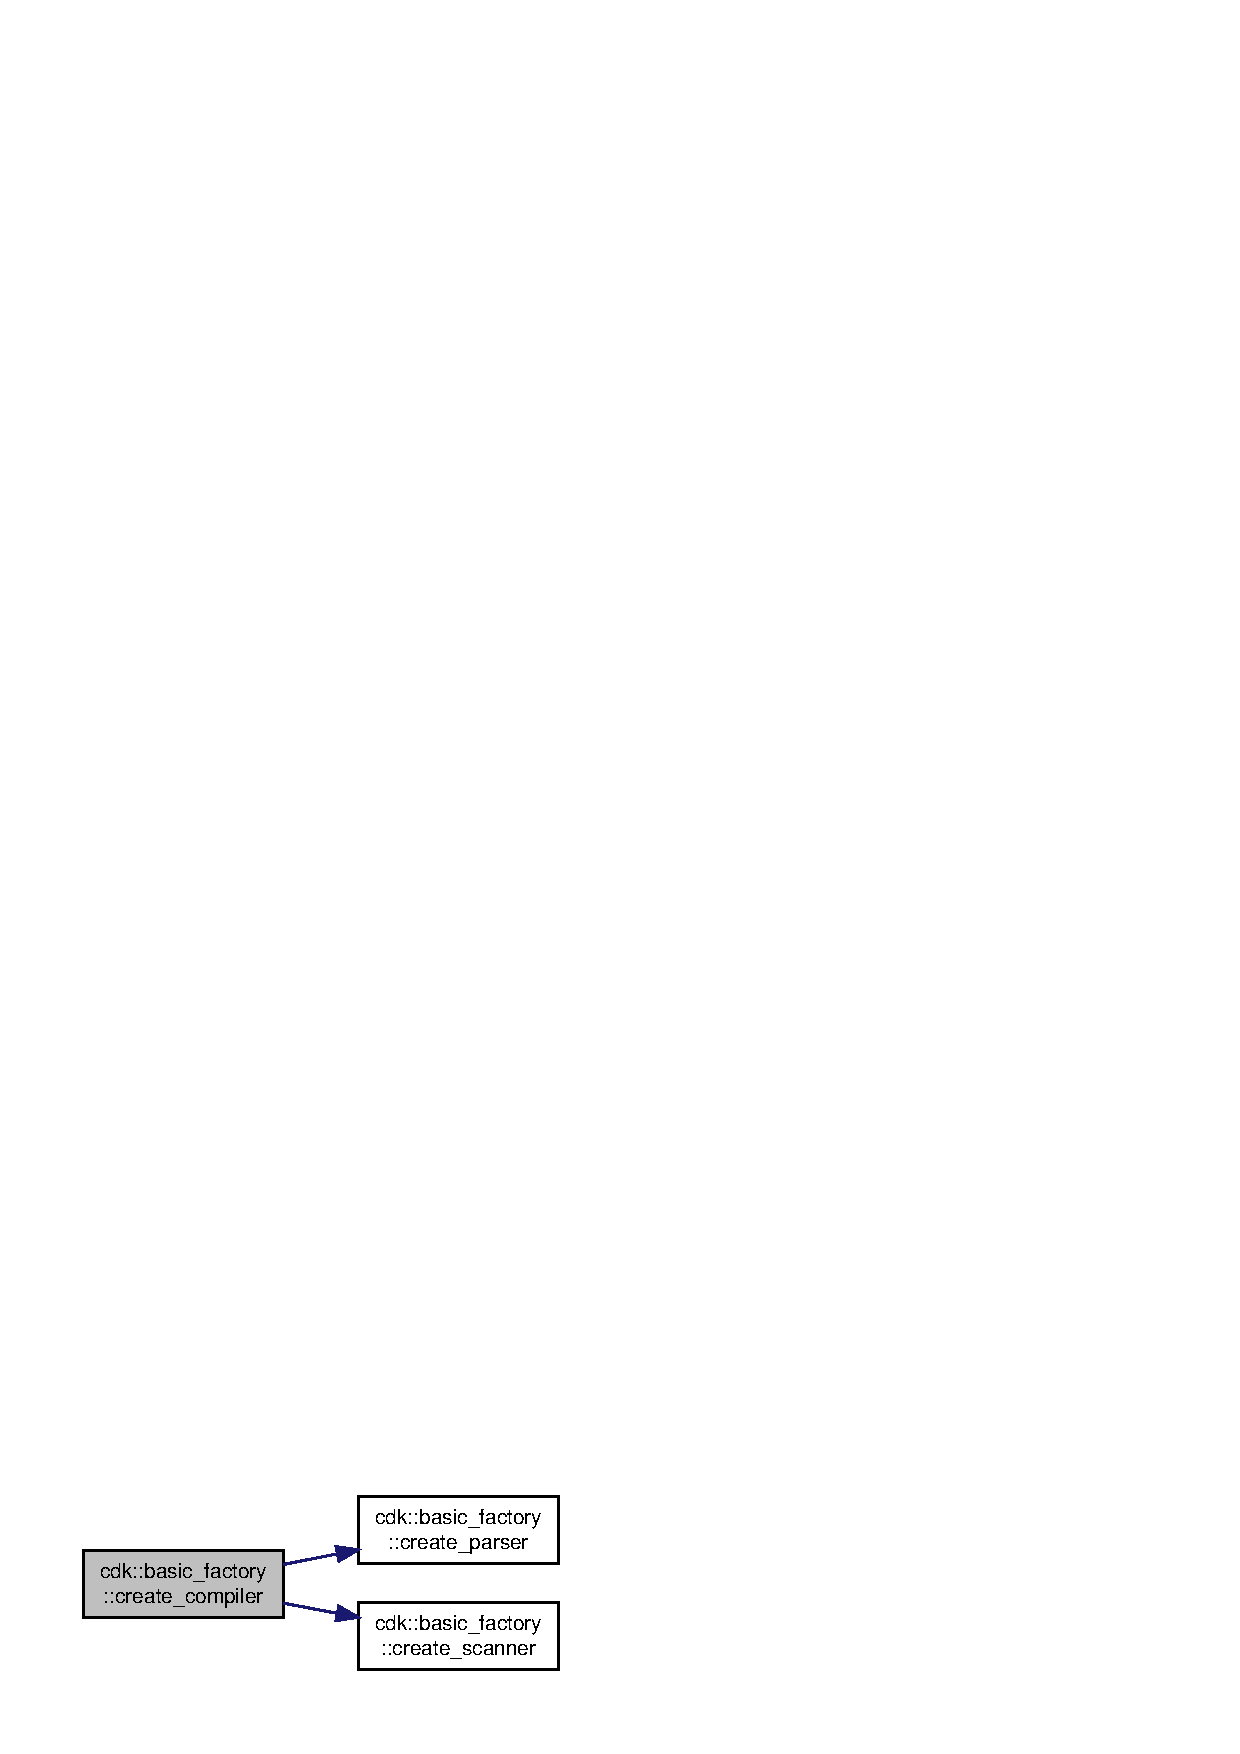
\includegraphics[width=272pt]{classcdk_1_1basic__factory_a883cf0f3e52b5a53b316914c74535de7_cgraph}
\end{center}
\end{figure}
\mbox{\label{classcdk_1_1basic__factory_afc8f88801455bf131cc4039271e6b741}} 
\index{cdk\+::basic\+\_\+factory@{cdk\+::basic\+\_\+factory}!create\+\_\+parser@{create\+\_\+parser}}
\index{create\+\_\+parser@{create\+\_\+parser}!cdk\+::basic\+\_\+factory@{cdk\+::basic\+\_\+factory}}
\subsubsection{create\+\_\+parser()}
{\footnotesize\ttfamily virtual std\+::shared\+\_\+ptr$<$\textbf{ basic\+\_\+parser}$>$ cdk\+::basic\+\_\+factory\+::create\+\_\+parser (\begin{DoxyParamCaption}{ }\end{DoxyParamCaption})\hspace{0.3cm}{\ttfamily [protected]}, {\ttfamily [pure virtual]}}

Create a parser object for a given language. 
\begin{DoxyParams}{Parameters}
{\em name} & name of the input file (for debug only) \\
\hline
\end{DoxyParams}
\begin{DoxyReturn}{Returns}
parser object pointer 
\end{DoxyReturn}
\begin{DoxySeeAlso}{See also}
create\+Compiler 
\end{DoxySeeAlso}


Implemented in \textbf{ cdk\+::yy\+\_\+factory$<$ Lexer\+Type $>$} \doxyref{}{p.}{classcdk_1_1yy__factory_a9a051ba49001a7dbb9822b64c45135e9}.



Referenced by create\+\_\+compiler().

\mbox{\label{classcdk_1_1basic__factory_a25f3a81be472baccf2ab5ffb2f363608}} 
\index{cdk\+::basic\+\_\+factory@{cdk\+::basic\+\_\+factory}!create\+\_\+scanner@{create\+\_\+scanner}}
\index{create\+\_\+scanner@{create\+\_\+scanner}!cdk\+::basic\+\_\+factory@{cdk\+::basic\+\_\+factory}}
\subsubsection{create\+\_\+scanner()}
{\footnotesize\ttfamily virtual std\+::shared\+\_\+ptr$<$\textbf{ basic\+\_\+scanner}$>$ cdk\+::basic\+\_\+factory\+::create\+\_\+scanner (\begin{DoxyParamCaption}{ }\end{DoxyParamCaption})\hspace{0.3cm}{\ttfamily [protected]}, {\ttfamily [pure virtual]}}

Create a scanner object for a given language. 
\begin{DoxyParams}{Parameters}
{\em name} & name of the input file (for debug only) \\
\hline
\end{DoxyParams}
\begin{DoxyReturn}{Returns}
scanner object pointer 
\end{DoxyReturn}
\begin{DoxySeeAlso}{See also}
create\+Compiler 
\end{DoxySeeAlso}


Implemented in \textbf{ cdk\+::yy\+\_\+factory$<$ Lexer\+Type $>$} \doxyref{}{p.}{classcdk_1_1yy__factory_a6132d875a397d6207727b070ed4155de}.



Referenced by create\+\_\+compiler().



The documentation for this class was generated from the following file\+:\begin{DoxyCompactItemize}
\item 
basic\+\_\+factory.\+h\end{DoxyCompactItemize}

\section{cdk\+:\+:basic\+\_\+node Class Reference}
\label{classcdk_1_1basic__node}\index{cdk\+::basic\+\_\+node@{cdk\+::basic\+\_\+node}}


{\ttfamily \#include $<$basic\+\_\+node.\+h$>$}



Inheritance diagram for cdk\+:\+:basic\+\_\+node\+:
\nopagebreak
\begin{figure}[H]
\begin{center}
\leavevmode
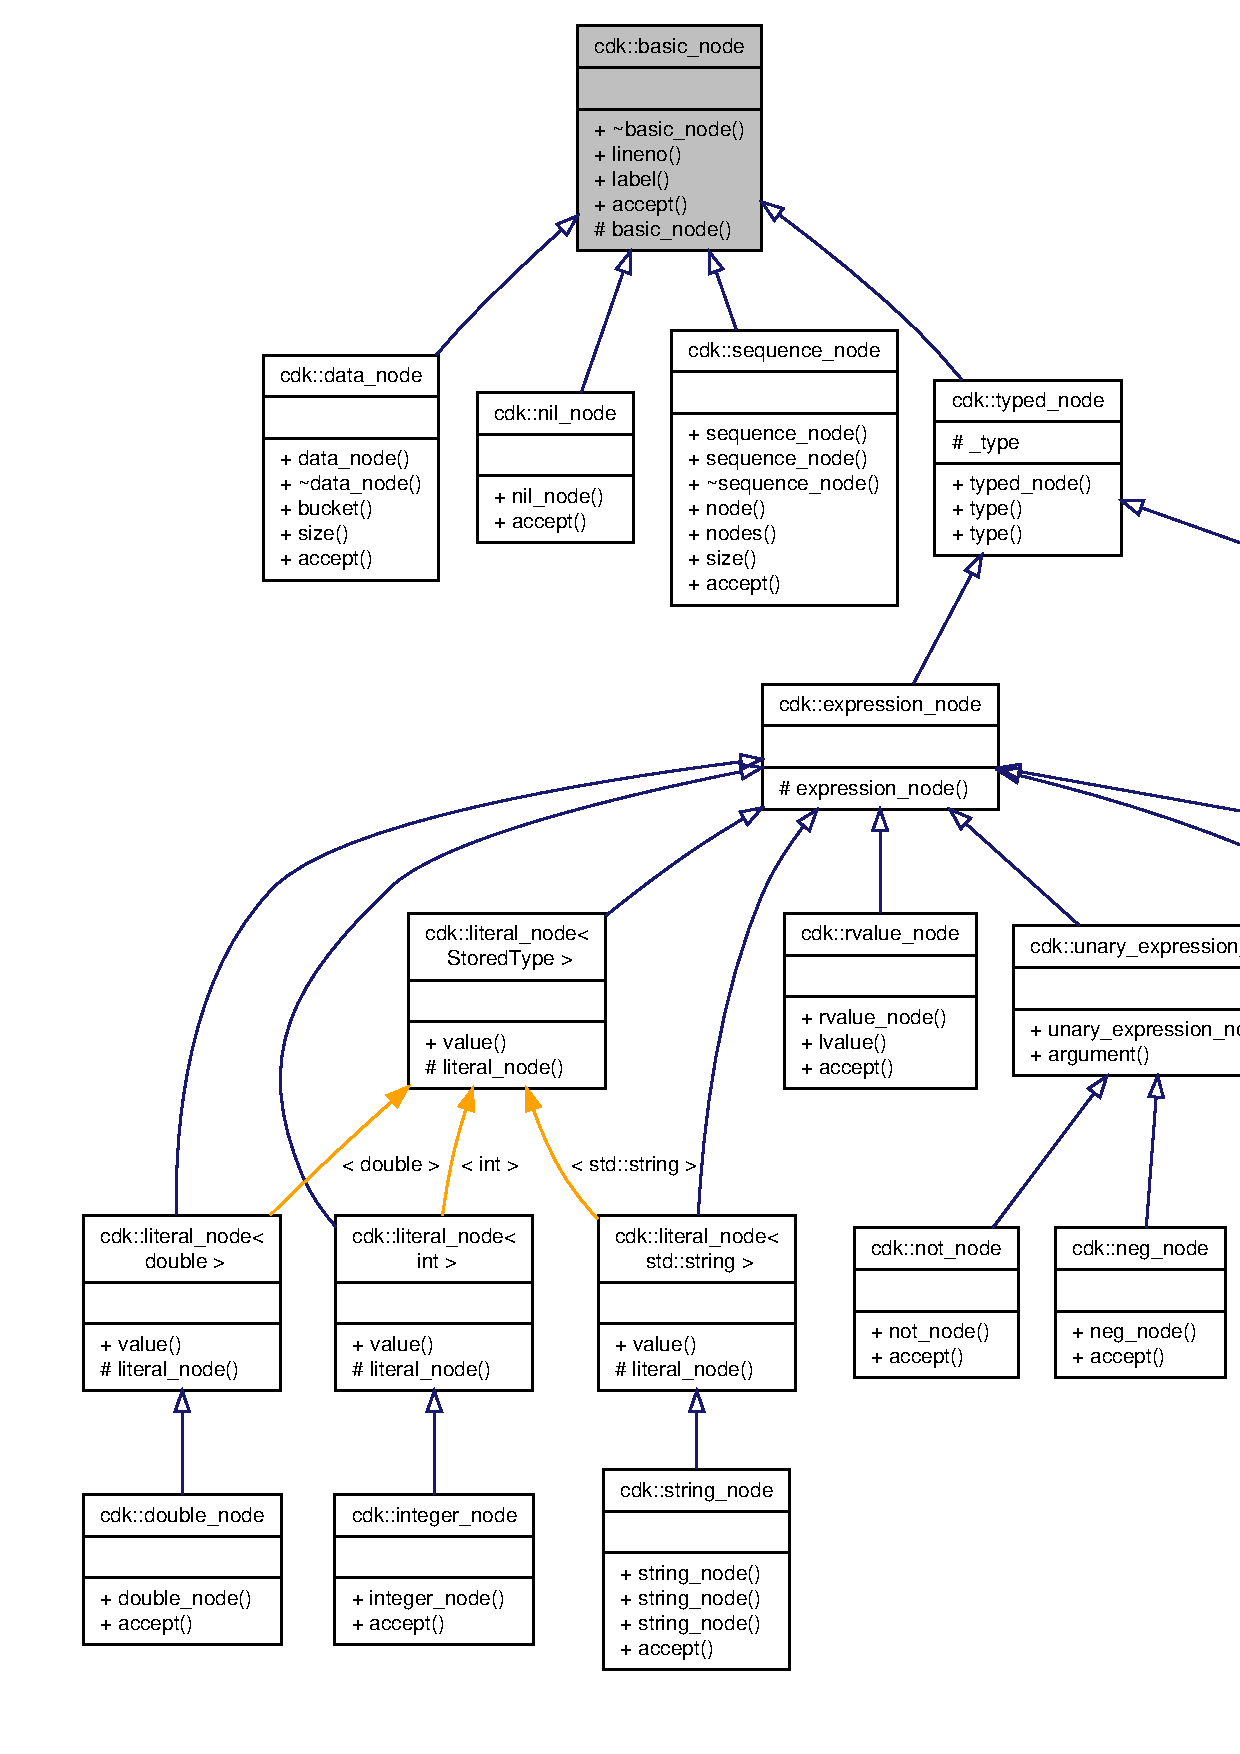
\includegraphics[width=350pt]{classcdk_1_1basic__node__inherit__graph}
\end{center}
\end{figure}


Collaboration diagram for cdk\+:\+:basic\+\_\+node\+:
\nopagebreak
\begin{figure}[H]
\begin{center}
\leavevmode
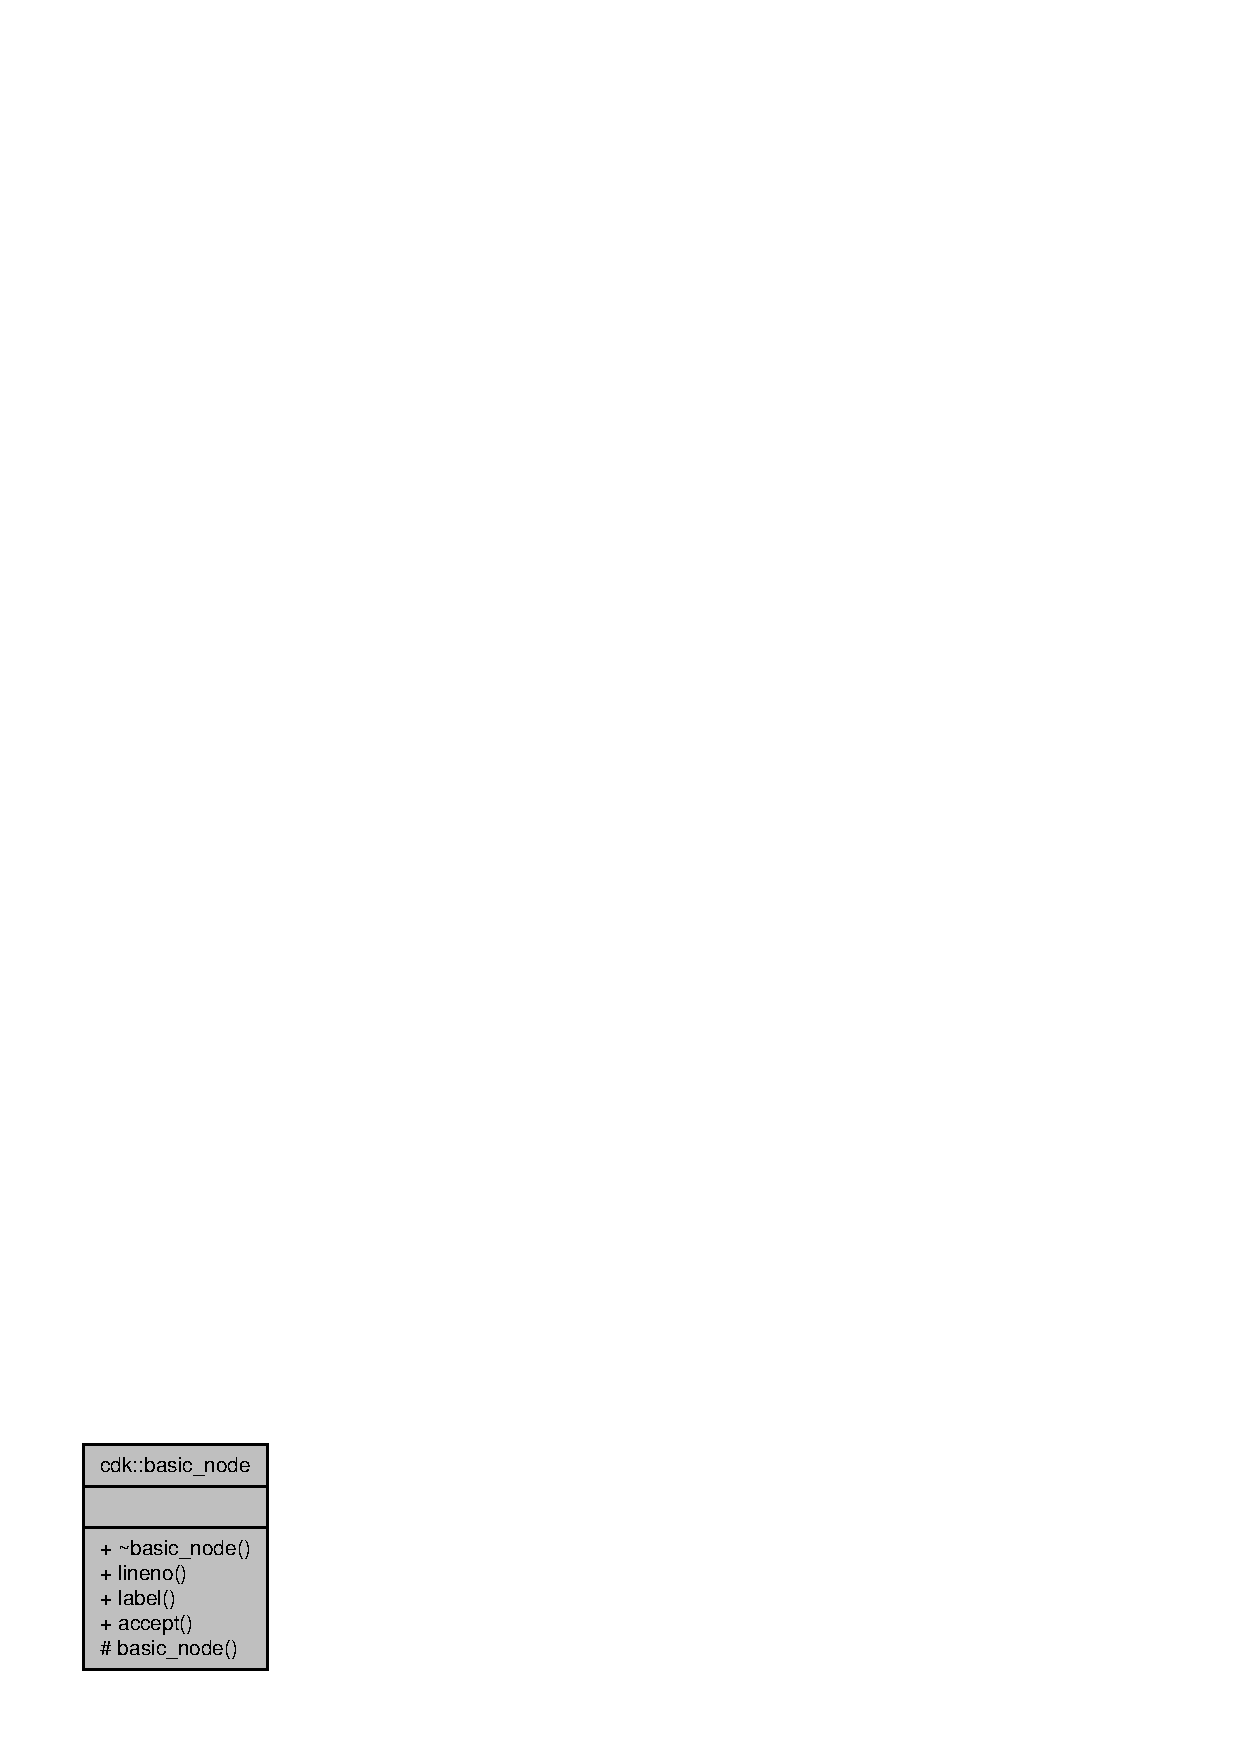
\includegraphics[width=132pt]{classcdk_1_1basic__node__coll__graph}
\end{center}
\end{figure}
\subsection*{Public Member Functions}
\begin{DoxyCompactItemize}
\item 
int \textbf{ lineno} () const
\item 
std\+::string \textbf{ label} () const
\item 
virtual void \textbf{ accept} (\textbf{ basic\+\_\+ast\+\_\+visitor} $\ast$sp, int level)=0
\end{DoxyCompactItemize}
\subsection*{Protected Member Functions}
\begin{DoxyCompactItemize}
\item 
\textbf{ basic\+\_\+node} (int \textbf{ lineno})
\end{DoxyCompactItemize}


\subsection{Detailed Description}
Class for describing A\+ST nodes. This is an abstract class and forms the root of the node hierarchy. The node hierarchy is organized in a structure according to the {\itshape Composite} design pattern\+: class {\ttfamily node} is the root of the hierarchy; class {\ttfamily simple} is a template for leaves holding simple (atomic) types; {\ttfamily composite} represents the recursive structure. Note that other recursion classes are possible by extending any of the classes in this family. 

Definition at line 20 of file basic\+\_\+node.\+h.



\subsection{Constructor \& Destructor Documentation}
\mbox{\label{classcdk_1_1basic__node_a4e09fec517e3a83503852de9e4fd5d72}} 
\index{cdk\+::basic\+\_\+node@{cdk\+::basic\+\_\+node}!basic\+\_\+node@{basic\+\_\+node}}
\index{basic\+\_\+node@{basic\+\_\+node}!cdk\+::basic\+\_\+node@{cdk\+::basic\+\_\+node}}
\subsubsection{basic\+\_\+node()}
{\footnotesize\ttfamily cdk\+::basic\+\_\+node\+::basic\+\_\+node (\begin{DoxyParamCaption}\item[{int}]{lineno }\end{DoxyParamCaption})\hspace{0.3cm}{\ttfamily [inline]}, {\ttfamily [protected]}}

Simple constructor.


\begin{DoxyParams}{Parameters}
{\em lineno} & the source code line number corresponding to the node \\
\hline
\end{DoxyParams}


Definition at line 29 of file basic\+\_\+node.\+h.



\subsection{Member Function Documentation}
\mbox{\label{classcdk_1_1basic__node_ab38adcbc95c46b809961278afae3bf05}} 
\index{cdk\+::basic\+\_\+node@{cdk\+::basic\+\_\+node}!accept@{accept}}
\index{accept@{accept}!cdk\+::basic\+\_\+node@{cdk\+::basic\+\_\+node}}
\subsubsection{accept()}
{\footnotesize\ttfamily virtual void cdk\+::basic\+\_\+node\+::accept (\begin{DoxyParamCaption}\item[{\textbf{ basic\+\_\+ast\+\_\+visitor} $\ast$}]{sp,  }\item[{int}]{level }\end{DoxyParamCaption})\hspace{0.3cm}{\ttfamily [pure virtual]}}

Every node must provide this method.


\begin{DoxyParams}{Parameters}
{\em sp} & semantic processor visitor \\
\hline
{\em level} & syntactic tree level \\
\hline
\end{DoxyParams}


Implemented in \textbf{ cdk\+::sequence\+\_\+node} \doxyref{}{p.}{classcdk_1_1sequence__node_a65774c75d4f946c18222043a14968190}, \textbf{ cdk\+::data\+\_\+node} \doxyref{}{p.}{classcdk_1_1data__node_a9d6d6f56201fdfbe965ec399ced60df8}, \textbf{ cdk\+::variable\+\_\+node} \doxyref{}{p.}{classcdk_1_1variable__node_a4f5516dfddf9a4a69aad199831ad92ce}, \textbf{ cdk\+::nil\+\_\+node} \doxyref{}{p.}{classcdk_1_1nil__node_a98fe1eb1acb00d40f91a75a18db2e86d}, \textbf{ cdk\+::assignment\+\_\+node} \doxyref{}{p.}{classcdk_1_1assignment__node_a02ccd8c51da2f61195e994db3f482c4f}, \textbf{ cdk\+::string\+\_\+node} \doxyref{}{p.}{classcdk_1_1string__node_a8ddaf8a19a75e2ff892eadd1606cb16f}, \textbf{ cdk\+::and\+\_\+node} \doxyref{}{p.}{classcdk_1_1and__node_a6bfbb0fa5db8f100c88b196c791135d7}, \textbf{ cdk\+::eq\+\_\+node} \doxyref{}{p.}{classcdk_1_1eq__node_ac874f2c13fc2f66ce23b08d99594368e}, \textbf{ cdk\+::not\+\_\+node} \doxyref{}{p.}{classcdk_1_1not__node_a7e4b13d01be3ae766b9678cfd626ecca}, \textbf{ cdk\+::or\+\_\+node} \doxyref{}{p.}{classcdk_1_1or__node_a3c9f8edad970cc80a65224710b56c5a2}, \textbf{ cdk\+::add\+\_\+node} \doxyref{}{p.}{classcdk_1_1add__node_a5a0a7fd1aacfcf589233c9b1cdda59d1}, \textbf{ cdk\+::ge\+\_\+node} \doxyref{}{p.}{classcdk_1_1ge__node_a758ad0281c1e925aab356d757bedce40}, \textbf{ cdk\+::gt\+\_\+node} \doxyref{}{p.}{classcdk_1_1gt__node_ab1104710ad583f4b13d397bf33b2f9f5}, \textbf{ cdk\+::le\+\_\+node} \doxyref{}{p.}{classcdk_1_1le__node_a4d3a01246f47dcb95ab7535a9047c9d6}, \textbf{ cdk\+::lt\+\_\+node} \doxyref{}{p.}{classcdk_1_1lt__node_a6af8ca3130c12e7a38860c9e92aaaa97}, \textbf{ cdk\+::mod\+\_\+node} \doxyref{}{p.}{classcdk_1_1mod__node_a990120f568275fb78d9adf66ec46434a}, \textbf{ cdk\+::mul\+\_\+node} \doxyref{}{p.}{classcdk_1_1mul__node_a82daadfc3194683a75c2e0630d09318d}, \textbf{ cdk\+::ne\+\_\+node} \doxyref{}{p.}{classcdk_1_1ne__node_a66ac549e9cc152c1d4c23dfe0c3c3830}, \textbf{ cdk\+::rvalue\+\_\+node} \doxyref{}{p.}{classcdk_1_1rvalue__node_ad43a4e9cdb648a1a21600c9a5ad90b94}, \textbf{ cdk\+::sub\+\_\+node} \doxyref{}{p.}{classcdk_1_1sub__node_a6200490aef72dc9483ac91047ba78e12}, \textbf{ cdk\+::div\+\_\+node} \doxyref{}{p.}{classcdk_1_1div__node_a18fdb1b825aeba112a607964f3901a6d}, \textbf{ cdk\+::double\+\_\+node} \doxyref{}{p.}{classcdk_1_1double__node_a3338941e9e94a4f88df4a418092c1ec8}, \textbf{ cdk\+::integer\+\_\+node} \doxyref{}{p.}{classcdk_1_1integer__node_a6b47d4c572b80bbaed62604a8c68788d}, and \textbf{ cdk\+::neg\+\_\+node} \doxyref{}{p.}{classcdk_1_1neg__node_ac49b8a32b9edaccfe38000cdb23d44c2}.

\mbox{\label{classcdk_1_1basic__node_afb8d57ad8e86d8392d6c67b2f8c04218}} 
\index{cdk\+::basic\+\_\+node@{cdk\+::basic\+\_\+node}!label@{label}}
\index{label@{label}!cdk\+::basic\+\_\+node@{cdk\+::basic\+\_\+node}}
\subsubsection{label()}
{\footnotesize\ttfamily std\+::string cdk\+::basic\+\_\+node\+::label (\begin{DoxyParamCaption}{ }\end{DoxyParamCaption}) const\hspace{0.3cm}{\ttfamily [inline]}}

\begin{DoxyReturn}{Returns}
the label of the node (i.\+e., it\textquotesingle{}s class) 
\end{DoxyReturn}


Definition at line 46 of file basic\+\_\+node.\+h.

\mbox{\label{classcdk_1_1basic__node_a845822a9c2f758b116086b532e20589c}} 
\index{cdk\+::basic\+\_\+node@{cdk\+::basic\+\_\+node}!lineno@{lineno}}
\index{lineno@{lineno}!cdk\+::basic\+\_\+node@{cdk\+::basic\+\_\+node}}
\subsubsection{lineno()}
{\footnotesize\ttfamily int cdk\+::basic\+\_\+node\+::lineno (\begin{DoxyParamCaption}{ }\end{DoxyParamCaption}) const\hspace{0.3cm}{\ttfamily [inline]}}

\begin{DoxyReturn}{Returns}
the line number of the corresponding source code 
\end{DoxyReturn}


Definition at line 39 of file basic\+\_\+node.\+h.



The documentation for this class was generated from the following file\+:\begin{DoxyCompactItemize}
\item 
ast/basic\+\_\+node.\+h\end{DoxyCompactItemize}

\section{cdk\+:\+:basic\+\_\+parser Class Reference}
\label{classcdk_1_1basic__parser}\index{cdk\+::basic\+\_\+parser@{cdk\+::basic\+\_\+parser}}


Inheritance diagram for cdk\+:\+:basic\+\_\+parser\+:
\nopagebreak
\begin{figure}[H]
\begin{center}
\leavevmode
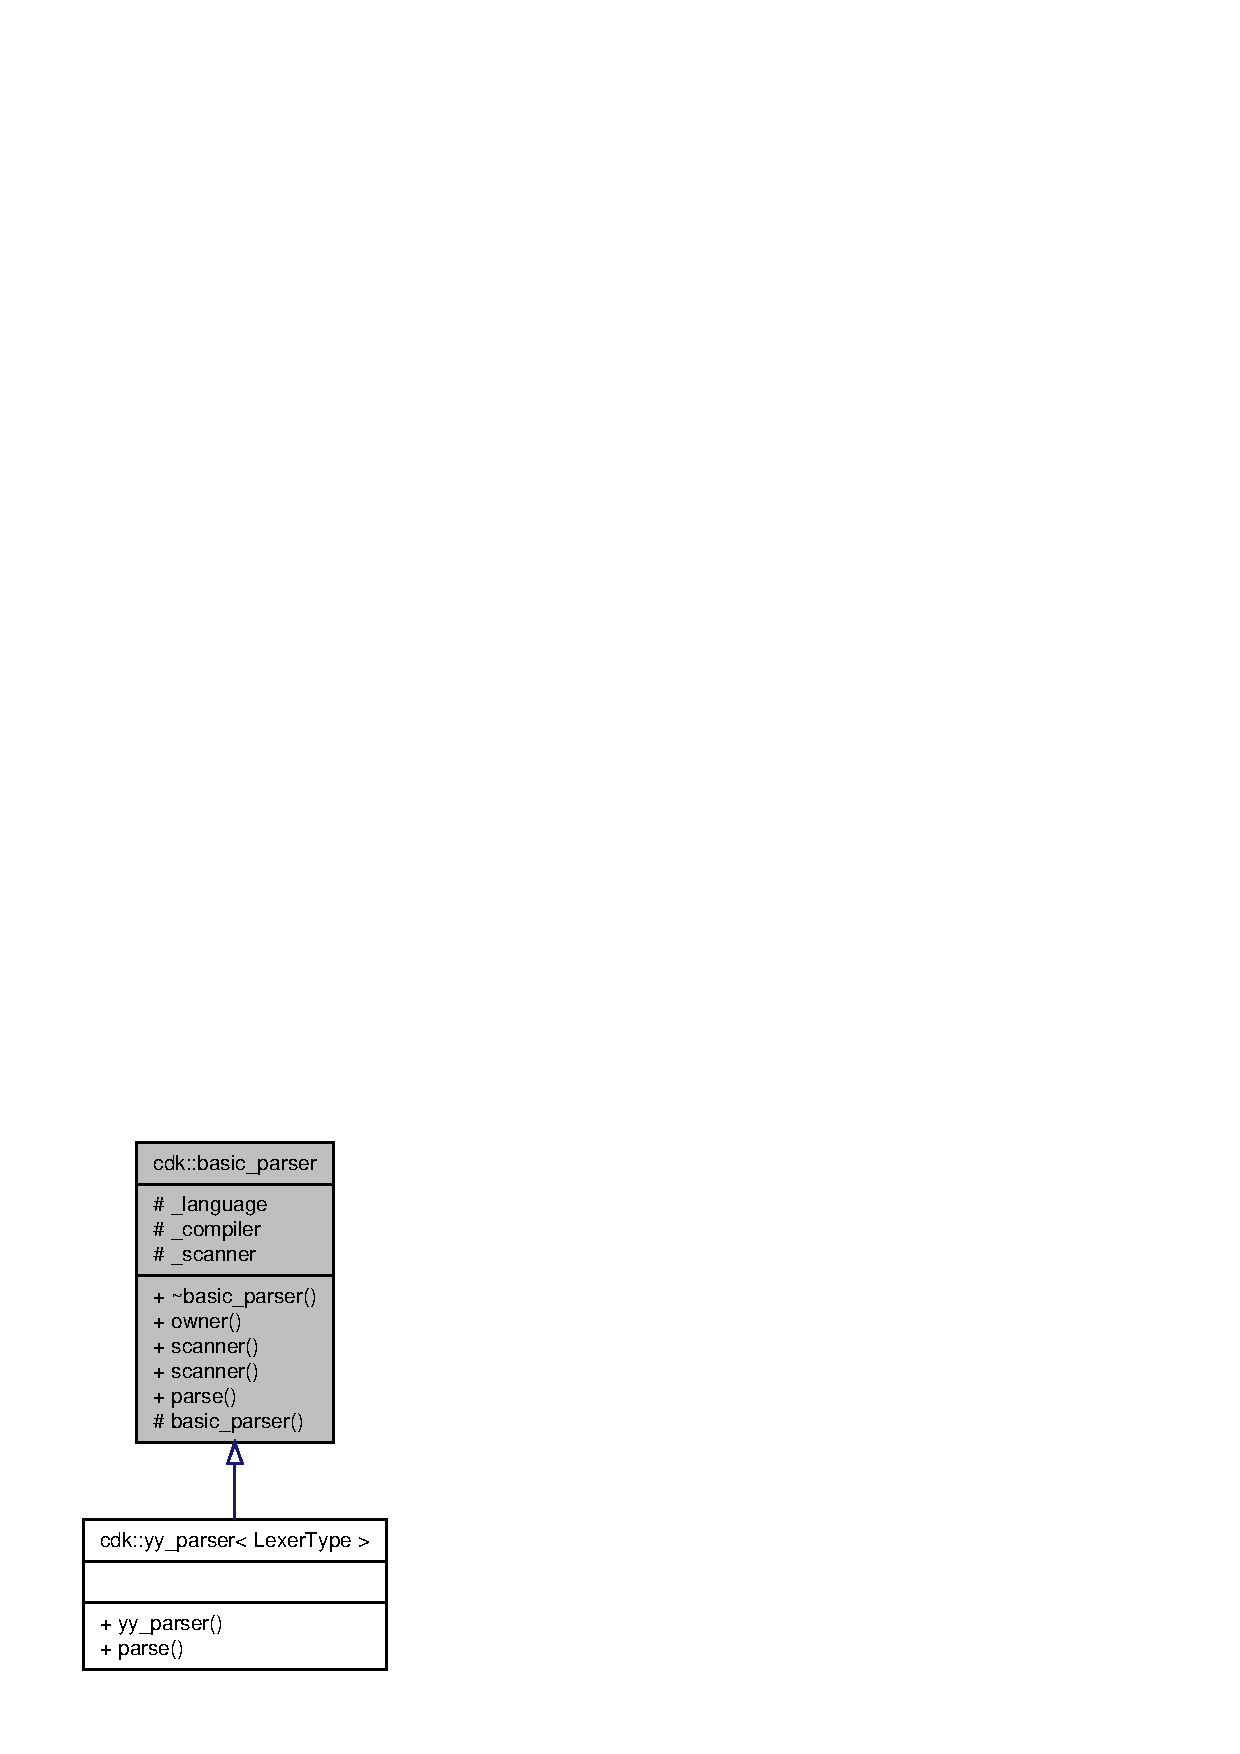
\includegraphics[width=189pt]{classcdk_1_1basic__parser__inherit__graph}
\end{center}
\end{figure}


Collaboration diagram for cdk\+:\+:basic\+\_\+parser\+:
\nopagebreak
\begin{figure}[H]
\begin{center}
\leavevmode
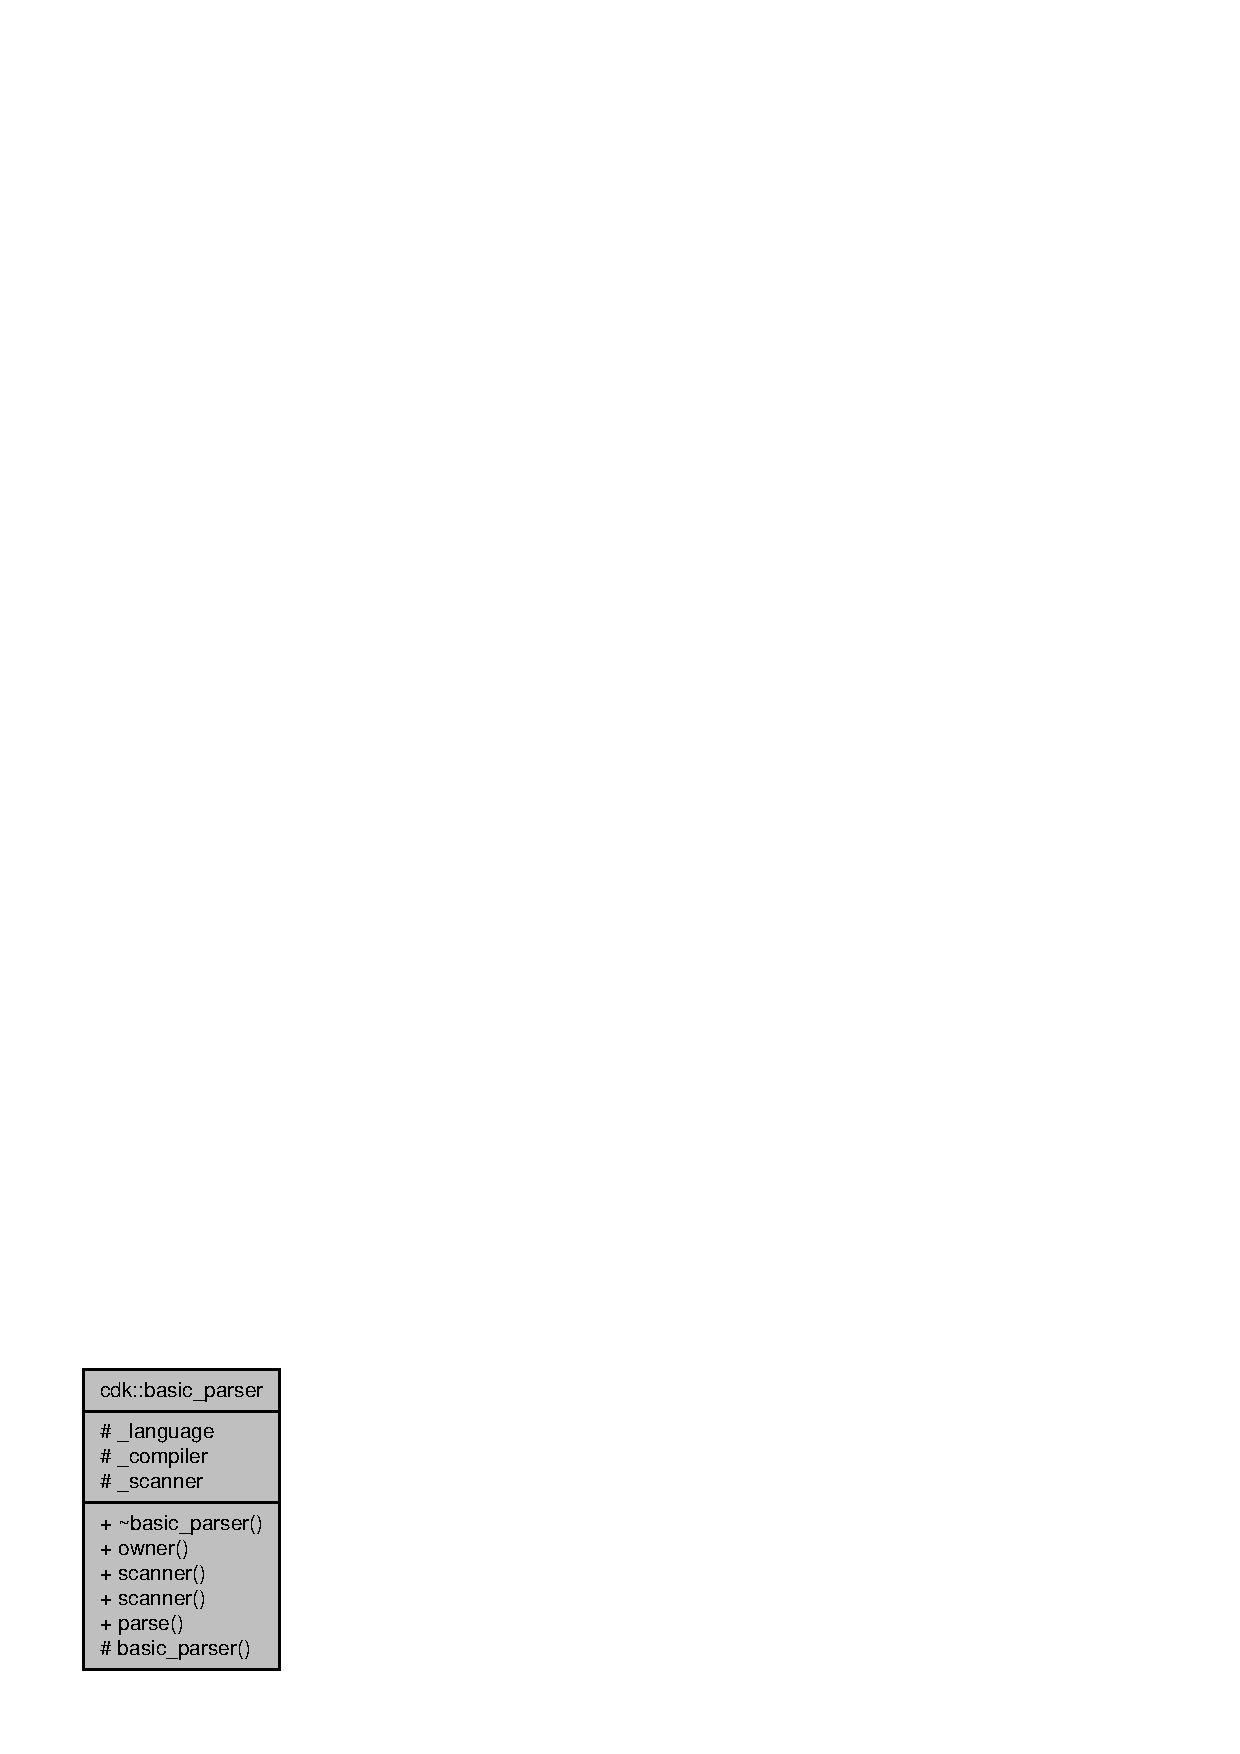
\includegraphics[width=138pt]{classcdk_1_1basic__parser__coll__graph}
\end{center}
\end{figure}
\subsection*{Public Member Functions}
\begin{DoxyCompactItemize}
\item 
\mbox{\label{classcdk_1_1basic__parser_a536c2274f7b00c0e17858b0ee1a400d6}} 
std\+::shared\+\_\+ptr$<$ \textbf{ compiler} $>$ {\bfseries owner} ()
\item 
\mbox{\label{classcdk_1_1basic__parser_a68543c111a7fef48ebe70c47b02ead09}} 
std\+::shared\+\_\+ptr$<$ \textbf{ basic\+\_\+scanner} $>$ {\bfseries scanner} ()
\item 
\mbox{\label{classcdk_1_1basic__parser_acc2215d959879e6fbac2f3e505c6bc03}} 
void {\bfseries scanner} (std\+::shared\+\_\+ptr$<$ \textbf{ basic\+\_\+scanner} $>$ scanner)
\item 
virtual int \textbf{ parse} ()=0
\end{DoxyCompactItemize}
\subsection*{Protected Member Functions}
\begin{DoxyCompactItemize}
\item 
\mbox{\label{classcdk_1_1basic__parser_a11506116556681fc7fbfe4a974ec0b34}} 
{\bfseries basic\+\_\+parser} (const std\+::string \&language, std\+::shared\+\_\+ptr$<$ \textbf{ basic\+\_\+scanner} $>$ scanner)
\end{DoxyCompactItemize}
\subsection*{Protected Attributes}
\begin{DoxyCompactItemize}
\item 
\mbox{\label{classcdk_1_1basic__parser_a1c97f24997ae2bceeae4822e32a449e4}} 
const std\+::string {\bfseries \+\_\+language} = \char`\"{}\char`\"{}
\item 
\mbox{\label{classcdk_1_1basic__parser_a1071aa82583cd806add631b8453fbfb1}} 
std\+::shared\+\_\+ptr$<$ \textbf{ compiler} $>$ {\bfseries \+\_\+compiler} = nullptr
\item 
\mbox{\label{classcdk_1_1basic__parser_aa88b520cd9bc71be71c9ad9dedbd9895}} 
std\+::shared\+\_\+ptr$<$ \textbf{ basic\+\_\+scanner} $>$ {\bfseries \+\_\+scanner} = nullptr
\end{DoxyCompactItemize}
\subsection*{Friends}
\begin{DoxyCompactItemize}
\item 
\mbox{\label{classcdk_1_1basic__parser_a6450bc9182feebc4fe52fbf86fa0ba40}} 
class {\bfseries compiler}
\end{DoxyCompactItemize}


\subsection{Detailed Description}


Definition at line 12 of file basic\+\_\+parser.\+h.



\subsection{Member Function Documentation}
\mbox{\label{classcdk_1_1basic__parser_a974c94ef048509a80bd042ee9c783513}} 
\index{cdk\+::basic\+\_\+parser@{cdk\+::basic\+\_\+parser}!parse@{parse}}
\index{parse@{parse}!cdk\+::basic\+\_\+parser@{cdk\+::basic\+\_\+parser}}
\subsubsection{parse()}
{\footnotesize\ttfamily virtual int cdk\+::basic\+\_\+parser\+::parse (\begin{DoxyParamCaption}{ }\end{DoxyParamCaption})\hspace{0.3cm}{\ttfamily [pure virtual]}}

Parse algorithm\+: the compiler object stores the result. 
\begin{DoxyParams}{Parameters}
{\em compiler} & the compiler object this parser belongs to. \\
\hline
\end{DoxyParams}
\begin{DoxyReturn}{Returns}
true if the operation is successful 
\end{DoxyReturn}


Implemented in \textbf{ cdk\+::yy\+\_\+parser$<$ Lexer\+Type $>$} \doxyref{}{p.}{classcdk_1_1yy__parser_a998a98a7b38a6772fb24ae0eeb87ef17}.



The documentation for this class was generated from the following file\+:\begin{DoxyCompactItemize}
\item 
basic\+\_\+parser.\+h\end{DoxyCompactItemize}

\section{cdk\+:\+:basic\+\_\+postfix\+\_\+emitter Class Reference}
\label{classcdk_1_1basic__postfix__emitter}\index{cdk\+::basic\+\_\+postfix\+\_\+emitter@{cdk\+::basic\+\_\+postfix\+\_\+emitter}}


{\ttfamily \#include $<$basic\+\_\+postfix\+\_\+emitter.\+h$>$}



Inheritance diagram for cdk\+:\+:basic\+\_\+postfix\+\_\+emitter\+:
\nopagebreak
\begin{figure}[H]
\begin{center}
\leavevmode
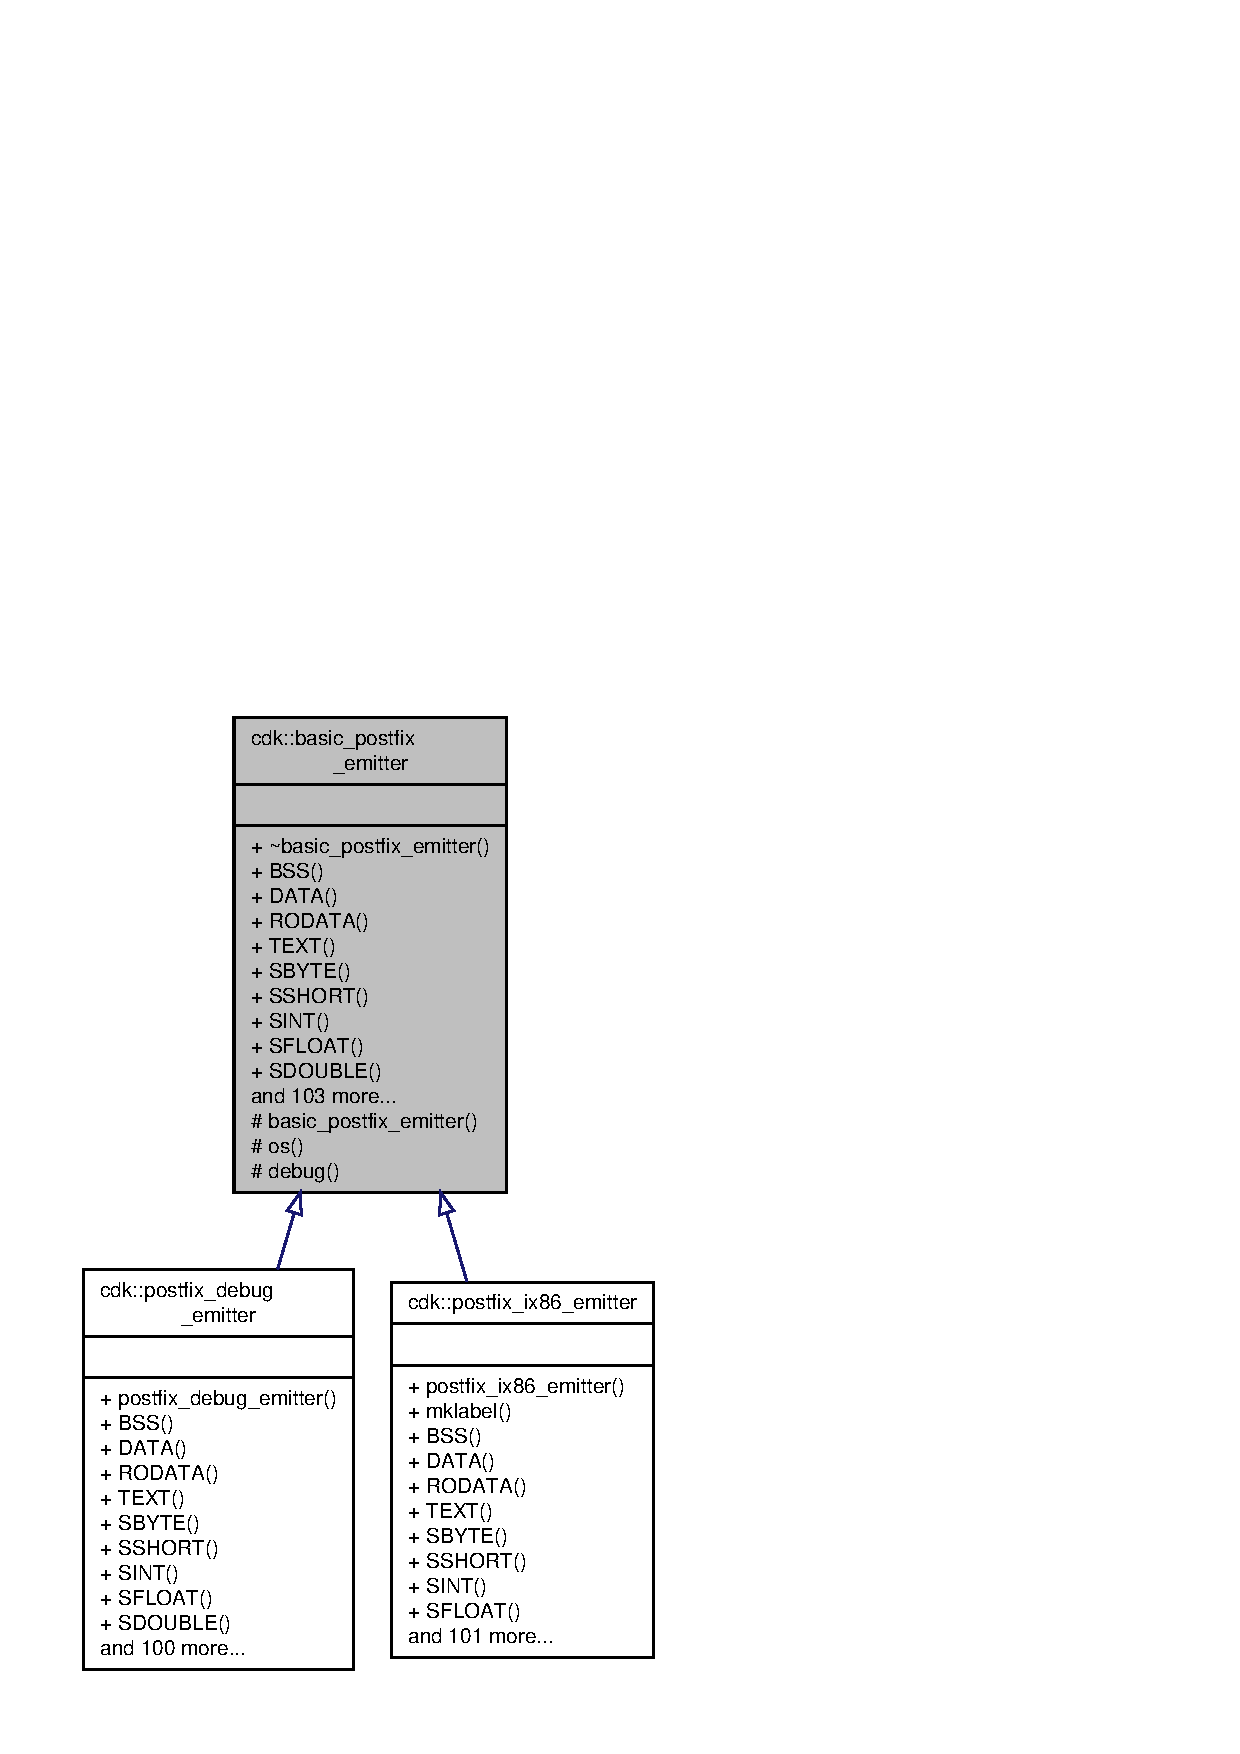
\includegraphics[width=318pt]{classcdk_1_1basic__postfix__emitter__inherit__graph}
\end{center}
\end{figure}


Collaboration diagram for cdk\+:\+:basic\+\_\+postfix\+\_\+emitter\+:
\nopagebreak
\begin{figure}[H]
\begin{center}
\leavevmode
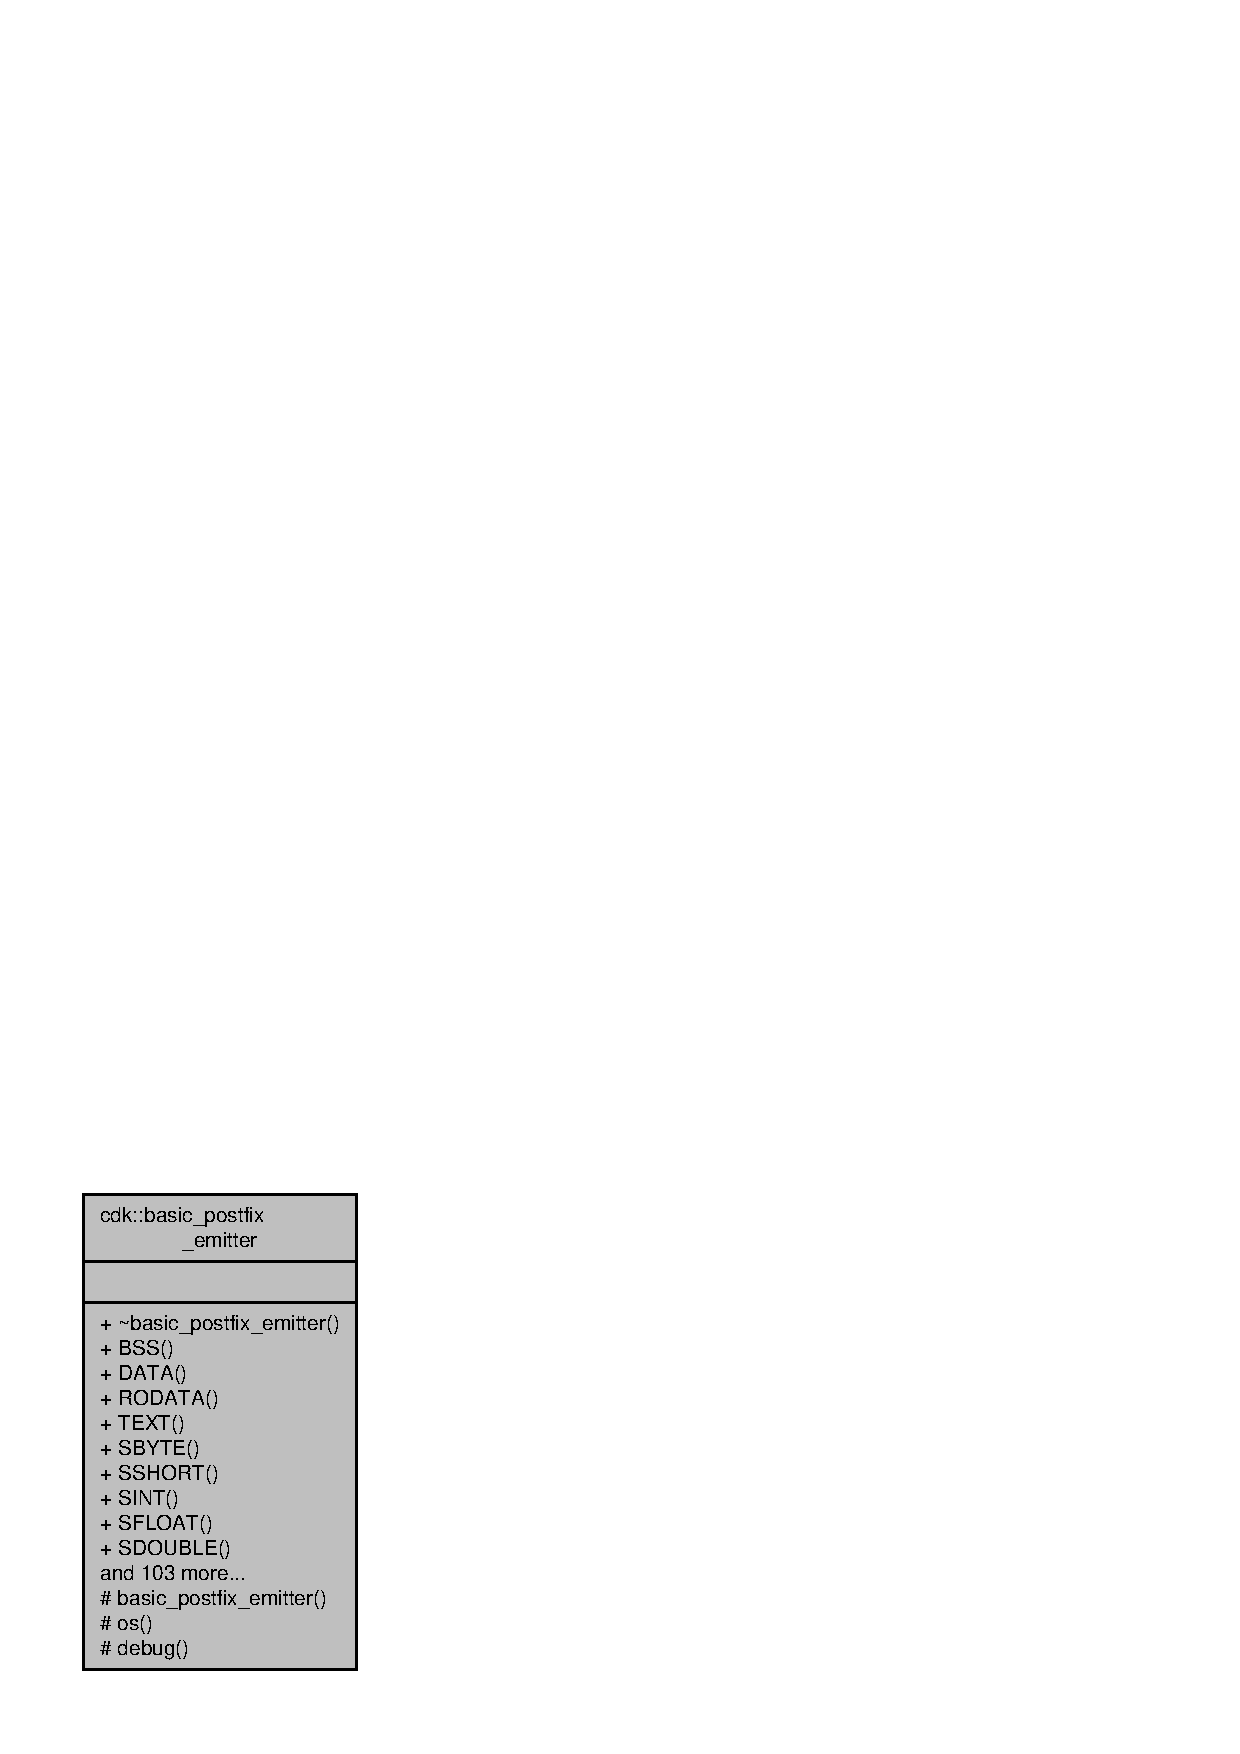
\includegraphics[width=175pt]{classcdk_1_1basic__postfix__emitter__coll__graph}
\end{center}
\end{figure}
\subsection*{Public Member Functions}
\begin{DoxyCompactItemize}
\item 
virtual \textbf{ $\sim$basic\+\_\+postfix\+\_\+emitter} ()
\item 
virtual void \textbf{ B\+SS} ()=0
\item 
virtual void \textbf{ D\+A\+TA} ()=0
\item 
virtual void \textbf{ R\+O\+D\+A\+TA} ()=0
\item 
virtual void \textbf{ T\+E\+XT} ()=0
\item 
virtual void \textbf{ S\+B\+Y\+TE} (char value)=0
\item 
virtual void \textbf{ S\+S\+H\+O\+RT} (short value)=0
\item 
virtual void \textbf{ S\+I\+NT} (int value)=0
\item 
virtual void \textbf{ S\+F\+L\+O\+AT} (float value)=0
\item 
virtual void \textbf{ S\+D\+O\+U\+B\+LE} (double value)=0
\item 
virtual void \textbf{ S\+S\+T\+R\+I\+NG} (std\+::string value)=0
\item 
virtual void \textbf{ S\+A\+L\+L\+OC} (int value)=0
\item 
virtual void \textbf{ S\+A\+D\+DR} (std\+::string label)=0
\item 
virtual void \textbf{ A\+L\+I\+GN} ()=0
\item 
virtual void \textbf{ L\+A\+B\+EL} (std\+::string label)=0
\item 
virtual void \textbf{ E\+X\+T\+E\+RN} (std\+::string label)=0
\item 
virtual void \textbf{ G\+L\+O\+B\+AL} (const char $\ast$label, std\+::string type)=0
\item 
virtual void \textbf{ G\+L\+O\+B\+AL} (std\+::string label, std\+::string type)=0
\item 
virtual void \textbf{ A\+D\+DR} (std\+::string label)=0
\item 
virtual void \textbf{ A\+D\+D\+RA} (std\+::string label)=0
\item 
virtual void \textbf{ A\+D\+D\+RV} (std\+::string label)=0
\item 
virtual void \textbf{ L\+O\+C\+AL} (int offset)=0
\item 
virtual void \textbf{ L\+O\+CA} (int offset)=0
\item 
virtual void \textbf{ L\+O\+CV} (int offset)=0
\item 
virtual void \textbf{ L\+D\+B\+Y\+TE} ()=0
\item 
virtual void \textbf{ L\+D\+S\+H\+O\+RT} ()=0
\item 
virtual void \textbf{ L\+D\+I\+NT} ()=0
\item 
virtual void \textbf{ L\+D\+F\+L\+O\+AT} ()=0
\item 
virtual void \textbf{ L\+D\+D\+O\+U\+B\+LE} ()=0
\item 
virtual void \textbf{ S\+T\+B\+Y\+TE} ()=0
\item 
virtual void \textbf{ S\+T\+S\+H\+O\+RT} ()=0
\item 
virtual void \textbf{ S\+T\+I\+NT} ()=0
\item 
virtual void \textbf{ S\+T\+F\+L\+O\+AT} ()=0
\item 
virtual void \textbf{ S\+T\+D\+O\+U\+B\+LE} ()=0
\item 
virtual void \textbf{ SP} ()=0
\item 
virtual void \textbf{ A\+L\+L\+OC} ()=0
\item 
virtual void \textbf{ D\+U\+P32} ()=0
\item 
virtual void \textbf{ D\+U\+P64} ()=0
\item 
virtual void \textbf{ S\+W\+A\+P32} ()=0
\item 
virtual void \textbf{ S\+W\+A\+P64} ()=0
\item 
virtual void \textbf{ I\+NT} (int value)=0
\item 
virtual void \textbf{ F\+L\+O\+AT} (float value)=0
\item 
virtual void \textbf{ D\+O\+U\+B\+LE} (double value)=0
\item 
virtual void \textbf{ N\+EG} ()=0
\item 
virtual void \textbf{ A\+DD} ()=0
\item 
virtual void \textbf{ S\+UB} ()=0
\item 
virtual void \textbf{ M\+UL} ()=0
\item 
virtual void \textbf{ D\+IV} ()=0
\item 
virtual void \textbf{ U\+D\+IV} ()=0
\item 
virtual void \textbf{ M\+OD} ()=0
\item 
virtual void \textbf{ U\+M\+OD} ()=0
\item 
virtual void \textbf{ D\+N\+EG} ()=0
\item 
virtual void \textbf{ D\+A\+DD} ()=0
\item 
virtual void \textbf{ D\+S\+UB} ()=0
\item 
virtual void \textbf{ D\+M\+UL} ()=0
\item 
virtual void \textbf{ D\+D\+IV} ()=0
\item 
virtual void \textbf{ I\+N\+CR} (int value)=0
\item 
virtual void \textbf{ D\+E\+CR} (int value)=0
\item 
virtual void \textbf{ D2F} ()=0
\item 
virtual void \textbf{ F2D} ()=0
\item 
virtual void \textbf{ D2I} ()=0
\item 
virtual void \textbf{ I2D} ()=0
\item 
virtual void \textbf{ EQ} ()=0
\item 
virtual void \textbf{ NE} ()=0
\item 
virtual void \textbf{ GT} ()=0
\item 
virtual void \textbf{ GE} ()=0
\item 
virtual void \textbf{ LE} ()=0
\item 
virtual void \textbf{ LT} ()=0
\item 
virtual void \textbf{ U\+GT} ()=0
\item 
virtual void \textbf{ U\+GE} ()=0
\item 
virtual void \textbf{ U\+LE} ()=0
\item 
virtual void \textbf{ U\+LT} ()=0
\item 
virtual void \textbf{ D\+C\+MP} ()=0
\item 
virtual void \textbf{ N\+OT} ()=0
\item 
virtual void \textbf{ A\+ND} ()=0
\item 
virtual void \textbf{ OR} ()=0
\item 
virtual void \textbf{ X\+OR} ()=0
\item 
virtual void \textbf{ R\+O\+TL} ()=0
\item 
virtual void \textbf{ R\+O\+TR} ()=0
\item 
virtual void \textbf{ S\+H\+TL} ()=0
\item 
virtual void \textbf{ S\+H\+T\+RU} ()=0
\item 
virtual void \textbf{ S\+H\+T\+RS} ()=0
\item 
virtual void \textbf{ E\+N\+T\+ER} (size\+\_\+t bytes)=0
\item 
virtual void \textbf{ S\+T\+A\+RT} ()=0
\item 
virtual void \textbf{ S\+T\+F\+V\+A\+L32} ()=0
\item 
virtual void \textbf{ S\+T\+F\+V\+A\+L64} ()=0
\item 
virtual void \textbf{ L\+E\+A\+VE} ()=0
\item 
virtual void \textbf{ R\+ET} ()=0
\item 
virtual void \textbf{ R\+E\+TN} (int bytes)=0
\item 
virtual void \textbf{ C\+A\+LL} (std\+::string label)=0
\item 
virtual void \textbf{ T\+R\+A\+SH} (int bytes)=0
\item 
virtual void \textbf{ L\+D\+F\+V\+A\+L32} ()=0
\item 
virtual void \textbf{ L\+D\+F\+V\+A\+L64} ()=0
\item 
\mbox{\label{classcdk_1_1basic__postfix__emitter_a6b69b6284da7299d71b0294ebbbaef60}} 
virtual void {\bfseries J\+MP} (std\+::string)=0
\item 
\mbox{\label{classcdk_1_1basic__postfix__emitter_acc0612c90a650f8d6badfdc259469c4d}} 
virtual void {\bfseries L\+E\+AP} ()=0
\item 
\mbox{\label{classcdk_1_1basic__postfix__emitter_a73d6febefcf7612357ca68a08b2e2741}} 
virtual void {\bfseries B\+R\+A\+N\+CH} ()=0
\item 
\mbox{\label{classcdk_1_1basic__postfix__emitter_a506bb21fb6863b19a05d9bea2e256d5d}} 
virtual void {\bfseries JZ} (std\+::string)=0
\item 
\mbox{\label{classcdk_1_1basic__postfix__emitter_aadecd1333b6d4396a92fb8c32564f97a}} 
virtual void {\bfseries J\+NZ} (std\+::string)=0
\item 
\mbox{\label{classcdk_1_1basic__postfix__emitter_a7f873798e8252e8f9a472cec2c053c5d}} 
virtual void {\bfseries J\+EQ} (std\+::string)=0
\item 
\mbox{\label{classcdk_1_1basic__postfix__emitter_a98b0fd0cfbcf3cf975cfdaf3ac5d746e}} 
virtual void {\bfseries J\+NE} (std\+::string)=0
\item 
\mbox{\label{classcdk_1_1basic__postfix__emitter_a2180960ed57e256bf497a17a85c1fa51}} 
virtual void {\bfseries J\+GT} (std\+::string)=0
\item 
\mbox{\label{classcdk_1_1basic__postfix__emitter_a8458f133392384872764c23027aac330}} 
virtual void {\bfseries J\+GE} (std\+::string)=0
\item 
\mbox{\label{classcdk_1_1basic__postfix__emitter_ad88845595e354161759d990cacd6e2e3}} 
virtual void {\bfseries J\+LE} (std\+::string)=0
\item 
\mbox{\label{classcdk_1_1basic__postfix__emitter_a921077c6fe62c12eab6ae6b23d6cdf55}} 
virtual void {\bfseries J\+LT} (std\+::string)=0
\item 
\mbox{\label{classcdk_1_1basic__postfix__emitter_aaec43a6275605c7a491a32d23a604a4e}} 
virtual void {\bfseries J\+U\+GT} (std\+::string)=0
\item 
\mbox{\label{classcdk_1_1basic__postfix__emitter_a3f4654e4cecf52974f45f157920cd5e6}} 
virtual void {\bfseries J\+U\+GE} (std\+::string)=0
\item 
\mbox{\label{classcdk_1_1basic__postfix__emitter_a28a2150f1163f498e1e1fcfd4b0f45bd}} 
virtual void {\bfseries J\+U\+LE} (std\+::string)=0
\item 
\mbox{\label{classcdk_1_1basic__postfix__emitter_abf375336538656c247b52cd7af80d1a1}} 
virtual void {\bfseries J\+U\+LT} (std\+::string)=0
\item 
\mbox{\label{classcdk_1_1basic__postfix__emitter_a8298c7d276b2b8ec49a2a70c8608d43f}} 
virtual void {\bfseries N\+IL} ()=0
\item 
\mbox{\label{classcdk_1_1basic__postfix__emitter_a8b45caa490a5b0aef1aa2a25cd3a163e}} 
virtual void {\bfseries N\+OP} ()=0
\item 
\mbox{\label{classcdk_1_1basic__postfix__emitter_a7bba236cdc3b4d05eb4426f782aeeae9}} 
virtual std\+::string {\bfseries N\+O\+NE} () const
\item 
\mbox{\label{classcdk_1_1basic__postfix__emitter_ac7968aa99d0ffc8be7803caeb6d73461}} 
virtual std\+::string {\bfseries F\+U\+NC} () const
\item 
\mbox{\label{classcdk_1_1basic__postfix__emitter_ad3a0d188cb982e039236a3b3daa05b89}} 
virtual std\+::string {\bfseries O\+BJ} () const
\end{DoxyCompactItemize}
\subsection*{Protected Member Functions}
\begin{DoxyCompactItemize}
\item 
\mbox{\label{classcdk_1_1basic__postfix__emitter_acaf970d10f218a088bd57ca6bcadce35}} 
{\bfseries basic\+\_\+postfix\+\_\+emitter} (std\+::shared\+\_\+ptr$<$ \textbf{ compiler} $>$ \&\textbf{ compiler})
\item 
\mbox{\label{classcdk_1_1basic__postfix__emitter_a34b69125c2b35e846461de6328894166}} 
std\+::ostream \& {\bfseries os} ()
\item 
\mbox{\label{classcdk_1_1basic__postfix__emitter_ab8a379fd593474bc165f8187d831affd}} 
bool {\bfseries debug} ()
\end{DoxyCompactItemize}


\subsection{Detailed Description}
The postfix code emitter defines an interface to be used by semantic analysers, as defined by the strategy design pattern. Specific implementations will provide the realization of the postfix commands for a particular target machine.

\paragraph*{Rotation and shift instructions}

Shift and rotation operations have as maximum value the number of bits of the underlying processor register (32 bits in a ix86-\/family processor). Safe operation for values above is not guaranteed.

These operations use two values from the stack\+: the value at the top specifies the number of bits to rotate/shift; the second from the top is the value to be rotated/shifted.

\paragraph*{Logical instructions}

Logical instructions perform logical operations using the elements at the top of the stack. Arguments are taken from the stack, the result is put on the stack.

\paragraph*{Type conversion instructions}

Type conversion instructions perform elementary type conversions. The conversions are from and to integers and simple and double precision floating point values.

\paragraph*{Integer comparison instructions}

The comparison instructions are binary operations that leave at the top of the stack 0 (zero) or 1 (one), depending on the result result of the comparison\+: respectively, {\ttfamily false} or {\ttfamily true}. The value may be directly used to perform conditional jumps (e.\+g., JZ, J\+NZ), that use the value of the top of the stack instead of relying on special processor registers ({\itshape flags}).

\paragraph*{Function definition instructions}

In a stack machine the arguments for a function call are already in the stack. Thus, it is not necessary to put them there (it is enough not to remove them). When building functions that conform to the C calling convetions, those arguments are destroyed by the caller, {\itshape after} the return of the callee, using {\ttfamily T\+R\+A\+SH}, stating the total size (i.\+e., for all arguments). Regarding the callee, it must create a distinct activation register {\ttfamily E\+N\+T\+ER} or {\ttfamily S\+T\+A\+RT}) and, when no longer needed, destroy it ({\ttfamily L\+E\+A\+VE}). The latter action must be performed immediately before returning control to the caller.

Similarly, to return values from a function, the callee must call {\ttfamily P\+OP} to store the return value in the accumulator register, so that it survives the destruction of the invocation context. The caller must call {\ttfamily P\+U\+SH}, to put the accumulator in the stack. An analogous procedure is valid for {\ttfamily D\+P\+O\+P/\+D\+P\+U\+SH} (for double precision floating point return values).

\paragraph*{Addressing instructions}

Note [{\itshape 4}] that these operations (A\+D\+DR, L\+O\+C\+AL) put at the top of the stack the symbol\textquotesingle{}s address, independently of its origin. O endereço pode posteriormente ser utilizado como ponteiro, obtido o valor nesse endereço (L\+O\+AD) ou guardar um valor nesse endereço (S\+T\+O\+RE). No entanto, nas duas últimas situações, devido à frequência com que ocorrem e o número de ciclos de relógio que levam a executar, podem ser substituídas com vantagem pela operações descritas em [{\itshape 10}].

\char`\"{}\+Quick opcodes\char`\"{} are shortcuts for groups of operations commonly used together. These opcodes may be made efficient by implementing them in different ways than the original set of high-\/level operations would suggest, i.\+e., the code generated by {\ttfamily A\+D\+D\+RV} may be more efficient than the code generated by {\ttfamily A\+D\+DR} followed by {\ttfamily L\+O\+AD}. Nevertheless, the outcome is the same.

\paragraph*{Load instructions}

The load instructions assume that the top of the stack contains an address pointing to the data to be read. Each load instruction will replace the address at the top of the stack with the contents of the position it points to. Load instructions differ only in what they load.

\paragraph*{Store instructions}

Store instructions assume the stack contains at the top the address where data is to be stored. That data is in the stack, immediately after (below) the address. Store instructions differ only in what they store.

\paragraph*{Labels}

In a declaration of a symbol common to more than one module, other modules may also contain common or external declarations. Nevertheless, only one initialized declaration is allowed. Declarations need not be associated with any particular segments.

In a declaration common to several modules, any number of modules may contain common or external declarations, but only one of them may contain an initialized declaration. A declaration does not need to be specified in a specific segment. 

Definition at line 106 of file basic\+\_\+postfix\+\_\+emitter.\+h.



\subsection{Constructor \& Destructor Documentation}
\mbox{\label{classcdk_1_1basic__postfix__emitter_a4379176e34cbebf1ed583cf1666a3273}} 
\index{cdk\+::basic\+\_\+postfix\+\_\+emitter@{cdk\+::basic\+\_\+postfix\+\_\+emitter}!````~basic\+\_\+postfix\+\_\+emitter@{$\sim$basic\+\_\+postfix\+\_\+emitter}}
\index{````~basic\+\_\+postfix\+\_\+emitter@{$\sim$basic\+\_\+postfix\+\_\+emitter}!cdk\+::basic\+\_\+postfix\+\_\+emitter@{cdk\+::basic\+\_\+postfix\+\_\+emitter}}
\subsubsection{$\sim$basic\+\_\+postfix\+\_\+emitter()}
{\footnotesize\ttfamily virtual cdk\+::basic\+\_\+postfix\+\_\+emitter\+::$\sim$basic\+\_\+postfix\+\_\+emitter (\begin{DoxyParamCaption}{ }\end{DoxyParamCaption})\hspace{0.3cm}{\ttfamily [inline]}, {\ttfamily [virtual]}}

Destructor\+: the only action is to flush the output stream. 

Definition at line 128 of file basic\+\_\+postfix\+\_\+emitter.\+h.



\subsection{Member Function Documentation}
\mbox{\label{classcdk_1_1basic__postfix__emitter_a166a0afe31c5b1249b45c8f909bad6a1}} 
\index{cdk\+::basic\+\_\+postfix\+\_\+emitter@{cdk\+::basic\+\_\+postfix\+\_\+emitter}!A\+DD@{A\+DD}}
\index{A\+DD@{A\+DD}!cdk\+::basic\+\_\+postfix\+\_\+emitter@{cdk\+::basic\+\_\+postfix\+\_\+emitter}}
\subsubsection{A\+D\+D()}
{\footnotesize\ttfamily virtual void cdk\+::basic\+\_\+postfix\+\_\+emitter\+::\+A\+DD (\begin{DoxyParamCaption}{ }\end{DoxyParamCaption})\hspace{0.3cm}{\ttfamily [pure virtual]}}

Arithmetic instruction\+: integer sum of two integer values. 

Implemented in \textbf{ cdk\+::postfix\+\_\+ix86\+\_\+emitter} \doxyref{}{p.}{classcdk_1_1postfix__ix86__emitter_afa0095dfa99f942fc5039e22e600d1fb}, and \textbf{ cdk\+::postfix\+\_\+debug\+\_\+emitter} \doxyref{}{p.}{classcdk_1_1postfix__debug__emitter_ad89ea3f47c8f5608662620122f1e72e7}.

\mbox{\label{classcdk_1_1basic__postfix__emitter_a7ba49b8d813f8a01b97f19b0296a9f73}} 
\index{cdk\+::basic\+\_\+postfix\+\_\+emitter@{cdk\+::basic\+\_\+postfix\+\_\+emitter}!A\+D\+DR@{A\+D\+DR}}
\index{A\+D\+DR@{A\+D\+DR}!cdk\+::basic\+\_\+postfix\+\_\+emitter@{cdk\+::basic\+\_\+postfix\+\_\+emitter}}
\subsubsection{A\+D\+D\+R()}
{\footnotesize\ttfamily virtual void cdk\+::basic\+\_\+postfix\+\_\+emitter\+::\+A\+D\+DR (\begin{DoxyParamCaption}\item[{std\+::string}]{label }\end{DoxyParamCaption})\hspace{0.3cm}{\ttfamily [pure virtual]}}

Absolute addressing instruction\+: puts the address of the name passed as argument at the top of the stack.

Absolute addressing {\ttfamily A\+D\+DR}) is performed using labels. Relative addressing ({\ttfamily L\+O\+C\+AL}) requires a frame pointer to work\+: the frame pointer defines an addressing reference.


\begin{DoxyParams}{Parameters}
{\em label} & is the name of the memory position. \\
\hline
\end{DoxyParams}
\begin{DoxySeeAlso}{See also}
\doxyref{L\+O\+C\+AL}{p.}{classcdk_1_1basic__postfix__emitter_a0c1ccb1039c9c837b26c47e70ceddbd8} 
\end{DoxySeeAlso}


Implemented in \textbf{ cdk\+::postfix\+\_\+ix86\+\_\+emitter} \doxyref{}{p.}{classcdk_1_1postfix__ix86__emitter_ad8548bd57ce5c8c4bd8590675d0e4d95}, and \textbf{ cdk\+::postfix\+\_\+debug\+\_\+emitter} \doxyref{}{p.}{classcdk_1_1postfix__debug__emitter_abffe1cc27420bea02cf55ed347f422d9}.

\mbox{\label{classcdk_1_1basic__postfix__emitter_aff6880030f5ffb52129f17b9ad21ce39}} 
\index{cdk\+::basic\+\_\+postfix\+\_\+emitter@{cdk\+::basic\+\_\+postfix\+\_\+emitter}!A\+D\+D\+RA@{A\+D\+D\+RA}}
\index{A\+D\+D\+RA@{A\+D\+D\+RA}!cdk\+::basic\+\_\+postfix\+\_\+emitter@{cdk\+::basic\+\_\+postfix\+\_\+emitter}}
\subsubsection{A\+D\+D\+R\+A()}
{\footnotesize\ttfamily virtual void cdk\+::basic\+\_\+postfix\+\_\+emitter\+::\+A\+D\+D\+RA (\begin{DoxyParamCaption}\item[{std\+::string}]{label }\end{DoxyParamCaption})\hspace{0.3cm}{\ttfamily [pure virtual]}}

Absolute addressing instruction\+: quick opcode\+: the same as the sequence A\+D\+D\+R(name); \doxyref{S\+T\+I\+N\+T()}{p.}{classcdk_1_1basic__postfix__emitter_aca97a9eff694c6912653ecd6accf7d24};


\begin{DoxyParams}{Parameters}
{\em label} & is the name of the memory position. \\
\hline
\end{DoxyParams}


Implemented in \textbf{ cdk\+::postfix\+\_\+ix86\+\_\+emitter} \doxyref{}{p.}{classcdk_1_1postfix__ix86__emitter_a94654f364ea4c96515d750ddbb98391c}, and \textbf{ cdk\+::postfix\+\_\+debug\+\_\+emitter} \doxyref{}{p.}{classcdk_1_1postfix__debug__emitter_a8df30d48a16f94510c65eae9cfd72e16}.

\mbox{\label{classcdk_1_1basic__postfix__emitter_a42f63442b1aece94dfb8e94f18500955}} 
\index{cdk\+::basic\+\_\+postfix\+\_\+emitter@{cdk\+::basic\+\_\+postfix\+\_\+emitter}!A\+D\+D\+RV@{A\+D\+D\+RV}}
\index{A\+D\+D\+RV@{A\+D\+D\+RV}!cdk\+::basic\+\_\+postfix\+\_\+emitter@{cdk\+::basic\+\_\+postfix\+\_\+emitter}}
\subsubsection{A\+D\+D\+R\+V()}
{\footnotesize\ttfamily virtual void cdk\+::basic\+\_\+postfix\+\_\+emitter\+::\+A\+D\+D\+RV (\begin{DoxyParamCaption}\item[{std\+::string}]{label }\end{DoxyParamCaption})\hspace{0.3cm}{\ttfamily [pure virtual]}}

Absolute addressing instruction\+: quick opcode\+: the same as the sequence A\+D\+D\+R(name); \doxyref{L\+D\+I\+N\+T()}{p.}{classcdk_1_1basic__postfix__emitter_aceb6564e7bcc2485bae28fd26882ebe3};


\begin{DoxyParams}{Parameters}
{\em label} & is the name of the memory position. \\
\hline
\end{DoxyParams}


Implemented in \textbf{ cdk\+::postfix\+\_\+ix86\+\_\+emitter} \doxyref{}{p.}{classcdk_1_1postfix__ix86__emitter_a38164c463e104aa55dbf2a7ebb0b9665}, and \textbf{ cdk\+::postfix\+\_\+debug\+\_\+emitter} \doxyref{}{p.}{classcdk_1_1postfix__debug__emitter_a76999bb6af72be3d4c13e18e159f16a3}.

\mbox{\label{classcdk_1_1basic__postfix__emitter_ac7faf0f5a5484fffa32a80b37659919a}} 
\index{cdk\+::basic\+\_\+postfix\+\_\+emitter@{cdk\+::basic\+\_\+postfix\+\_\+emitter}!A\+L\+I\+GN@{A\+L\+I\+GN}}
\index{A\+L\+I\+GN@{A\+L\+I\+GN}!cdk\+::basic\+\_\+postfix\+\_\+emitter@{cdk\+::basic\+\_\+postfix\+\_\+emitter}}
\subsubsection{A\+L\+I\+G\+N()}
{\footnotesize\ttfamily virtual void cdk\+::basic\+\_\+postfix\+\_\+emitter\+::\+A\+L\+I\+GN (\begin{DoxyParamCaption}{ }\end{DoxyParamCaption})\hspace{0.3cm}{\ttfamily [pure virtual]}}

Forces the alignment of code or data. 

Implemented in \textbf{ cdk\+::postfix\+\_\+ix86\+\_\+emitter} \doxyref{}{p.}{classcdk_1_1postfix__ix86__emitter_a3d3c4bdfa533f3dd8783242fee3b4cdd}, and \textbf{ cdk\+::postfix\+\_\+debug\+\_\+emitter} \doxyref{}{p.}{classcdk_1_1postfix__debug__emitter_ad4b58886979f969a269c5a075bf872f3}.

\mbox{\label{classcdk_1_1basic__postfix__emitter_ac9e4b7d03edd2bd1d5f2ca3c54c271a0}} 
\index{cdk\+::basic\+\_\+postfix\+\_\+emitter@{cdk\+::basic\+\_\+postfix\+\_\+emitter}!A\+L\+L\+OC@{A\+L\+L\+OC}}
\index{A\+L\+L\+OC@{A\+L\+L\+OC}!cdk\+::basic\+\_\+postfix\+\_\+emitter@{cdk\+::basic\+\_\+postfix\+\_\+emitter}}
\subsubsection{A\+L\+L\+O\+C()}
{\footnotesize\ttfamily virtual void cdk\+::basic\+\_\+postfix\+\_\+emitter\+::\+A\+L\+L\+OC (\begin{DoxyParamCaption}{ }\end{DoxyParamCaption})\hspace{0.3cm}{\ttfamily [pure virtual]}}

Allocates in the stack as many bytes as indicated by the value at the top of the stack.

Dynamic memory allocation in the stack, equivalent to a call to the C language {\ttfamily alloca} function, changes the offsets of temporary variables that may exist in the stack when the allocation is performed. Thus, it should only be used when no temporary variables exist, or when the full import of its actions is fully understood. 

Implemented in \textbf{ cdk\+::postfix\+\_\+ix86\+\_\+emitter} \doxyref{}{p.}{classcdk_1_1postfix__ix86__emitter_a66bc007ea64355d998b991994f2ff32b}, and \textbf{ cdk\+::postfix\+\_\+debug\+\_\+emitter} \doxyref{}{p.}{classcdk_1_1postfix__debug__emitter_a8f2c0e253f3cdc1f4550eb47d29f8e57}.

\mbox{\label{classcdk_1_1basic__postfix__emitter_a0e1eed9bc80ca1ace031793aeca088d2}} 
\index{cdk\+::basic\+\_\+postfix\+\_\+emitter@{cdk\+::basic\+\_\+postfix\+\_\+emitter}!A\+ND@{A\+ND}}
\index{A\+ND@{A\+ND}!cdk\+::basic\+\_\+postfix\+\_\+emitter@{cdk\+::basic\+\_\+postfix\+\_\+emitter}}
\subsubsection{A\+N\+D()}
{\footnotesize\ttfamily virtual void cdk\+::basic\+\_\+postfix\+\_\+emitter\+::\+A\+ND (\begin{DoxyParamCaption}{ }\end{DoxyParamCaption})\hspace{0.3cm}{\ttfamily [pure virtual]}}

Logical instructions\+: logical (bitwise) A\+ND operation. 

Implemented in \textbf{ cdk\+::postfix\+\_\+ix86\+\_\+emitter} \doxyref{}{p.}{classcdk_1_1postfix__ix86__emitter_ae57d4ba81a42454fb2522cba9f1a47dc}, and \textbf{ cdk\+::postfix\+\_\+debug\+\_\+emitter} \doxyref{}{p.}{classcdk_1_1postfix__debug__emitter_a340bb1d73ae964fa289f49269d35c6d4}.

\mbox{\label{classcdk_1_1basic__postfix__emitter_a42393ab0f62dc8737f30e6a9330a5392}} 
\index{cdk\+::basic\+\_\+postfix\+\_\+emitter@{cdk\+::basic\+\_\+postfix\+\_\+emitter}!B\+SS@{B\+SS}}
\index{B\+SS@{B\+SS}!cdk\+::basic\+\_\+postfix\+\_\+emitter@{cdk\+::basic\+\_\+postfix\+\_\+emitter}}
\subsubsection{B\+S\+S()}
{\footnotesize\ttfamily virtual void cdk\+::basic\+\_\+postfix\+\_\+emitter\+::\+B\+SS (\begin{DoxyParamCaption}{ }\end{DoxyParamCaption})\hspace{0.3cm}{\ttfamily [pure virtual]}}

Starts the data segment for uninitialized values. 

Implemented in \textbf{ cdk\+::postfix\+\_\+ix86\+\_\+emitter} \doxyref{}{p.}{classcdk_1_1postfix__ix86__emitter_a85beccc872f04963ba43cc4de6830afe}, and \textbf{ cdk\+::postfix\+\_\+debug\+\_\+emitter} \doxyref{}{p.}{classcdk_1_1postfix__debug__emitter_acd25ad2a4a5d04aba43fe9bc4332c83c}.

\mbox{\label{classcdk_1_1basic__postfix__emitter_a14660f946d6b4a3042611ae4345083e3}} 
\index{cdk\+::basic\+\_\+postfix\+\_\+emitter@{cdk\+::basic\+\_\+postfix\+\_\+emitter}!C\+A\+LL@{C\+A\+LL}}
\index{C\+A\+LL@{C\+A\+LL}!cdk\+::basic\+\_\+postfix\+\_\+emitter@{cdk\+::basic\+\_\+postfix\+\_\+emitter}}
\subsubsection{C\+A\+L\+L()}
{\footnotesize\ttfamily virtual void cdk\+::basic\+\_\+postfix\+\_\+emitter\+::\+C\+A\+LL (\begin{DoxyParamCaption}\item[{std\+::string}]{label }\end{DoxyParamCaption})\hspace{0.3cm}{\ttfamily [pure virtual]}}

Calls the named function. Stores the return address in the stack.


\begin{DoxyParams}{Parameters}
{\em label} & is the called function\textquotesingle{}s name. \\
\hline
\end{DoxyParams}


Implemented in \textbf{ cdk\+::postfix\+\_\+ix86\+\_\+emitter} \doxyref{}{p.}{classcdk_1_1postfix__ix86__emitter_a5a537579a545d3408abf8296609c96a0}, and \textbf{ cdk\+::postfix\+\_\+debug\+\_\+emitter} \doxyref{}{p.}{classcdk_1_1postfix__debug__emitter_a4236259d4784fe60158477fe6fe2f48b}.

\mbox{\label{classcdk_1_1basic__postfix__emitter_abbeaa516b69a9903db6f09884cd8dbf9}} 
\index{cdk\+::basic\+\_\+postfix\+\_\+emitter@{cdk\+::basic\+\_\+postfix\+\_\+emitter}!D2F@{D2F}}
\index{D2F@{D2F}!cdk\+::basic\+\_\+postfix\+\_\+emitter@{cdk\+::basic\+\_\+postfix\+\_\+emitter}}
\subsubsection{D2\+F()}
{\footnotesize\ttfamily virtual void cdk\+::basic\+\_\+postfix\+\_\+emitter\+::\+D2F (\begin{DoxyParamCaption}{ }\end{DoxyParamCaption})\hspace{0.3cm}{\ttfamily [pure virtual]}}

Type conversion instructions\+: converts from double precision floating point to simple precision floating point. 

Implemented in \textbf{ cdk\+::postfix\+\_\+ix86\+\_\+emitter} \doxyref{}{p.}{classcdk_1_1postfix__ix86__emitter_a434741141e010db162dc0b492498cbae}, and \textbf{ cdk\+::postfix\+\_\+debug\+\_\+emitter} \doxyref{}{p.}{classcdk_1_1postfix__debug__emitter_a085d1c721f6f12d595b80b17c52ade53}.

\mbox{\label{classcdk_1_1basic__postfix__emitter_a8feeef18145e463e5d9b88b1b44f4e0f}} 
\index{cdk\+::basic\+\_\+postfix\+\_\+emitter@{cdk\+::basic\+\_\+postfix\+\_\+emitter}!D2I@{D2I}}
\index{D2I@{D2I}!cdk\+::basic\+\_\+postfix\+\_\+emitter@{cdk\+::basic\+\_\+postfix\+\_\+emitter}}
\subsubsection{D2\+I()}
{\footnotesize\ttfamily virtual void cdk\+::basic\+\_\+postfix\+\_\+emitter\+::\+D2I (\begin{DoxyParamCaption}{ }\end{DoxyParamCaption})\hspace{0.3cm}{\ttfamily [pure virtual]}}

Type conversion instructions\+: converts from double precision floating point to integer. 

Implemented in \textbf{ cdk\+::postfix\+\_\+ix86\+\_\+emitter} \doxyref{}{p.}{classcdk_1_1postfix__ix86__emitter_af1139fd5b66be8e8b11464241bf2214c}, and \textbf{ cdk\+::postfix\+\_\+debug\+\_\+emitter} \doxyref{}{p.}{classcdk_1_1postfix__debug__emitter_a29ebf3c99df035bc6f00b24b443aa67b}.

\mbox{\label{classcdk_1_1basic__postfix__emitter_a49807e0402b6945cde85c0990c067e4c}} 
\index{cdk\+::basic\+\_\+postfix\+\_\+emitter@{cdk\+::basic\+\_\+postfix\+\_\+emitter}!D\+A\+DD@{D\+A\+DD}}
\index{D\+A\+DD@{D\+A\+DD}!cdk\+::basic\+\_\+postfix\+\_\+emitter@{cdk\+::basic\+\_\+postfix\+\_\+emitter}}
\subsubsection{D\+A\+D\+D()}
{\footnotesize\ttfamily virtual void cdk\+::basic\+\_\+postfix\+\_\+emitter\+::\+D\+A\+DD (\begin{DoxyParamCaption}{ }\end{DoxyParamCaption})\hspace{0.3cm}{\ttfamily [pure virtual]}}

Arithmetic instruction\+: floating point sum of two double values. 

Implemented in \textbf{ cdk\+::postfix\+\_\+ix86\+\_\+emitter} \doxyref{}{p.}{classcdk_1_1postfix__ix86__emitter_aaeebfd9f7c74d300bcba2c7c645e19e0}, and \textbf{ cdk\+::postfix\+\_\+debug\+\_\+emitter} \doxyref{}{p.}{classcdk_1_1postfix__debug__emitter_a121696d01d3b9707f12f637e901ebe5c}.

\mbox{\label{classcdk_1_1basic__postfix__emitter_af5ea780b17aad05db0301334d3ead1f8}} 
\index{cdk\+::basic\+\_\+postfix\+\_\+emitter@{cdk\+::basic\+\_\+postfix\+\_\+emitter}!D\+A\+TA@{D\+A\+TA}}
\index{D\+A\+TA@{D\+A\+TA}!cdk\+::basic\+\_\+postfix\+\_\+emitter@{cdk\+::basic\+\_\+postfix\+\_\+emitter}}
\subsubsection{D\+A\+T\+A()}
{\footnotesize\ttfamily virtual void cdk\+::basic\+\_\+postfix\+\_\+emitter\+::\+D\+A\+TA (\begin{DoxyParamCaption}{ }\end{DoxyParamCaption})\hspace{0.3cm}{\ttfamily [pure virtual]}}

Starts the data segment for initialized values. 

Implemented in \textbf{ cdk\+::postfix\+\_\+ix86\+\_\+emitter} \doxyref{}{p.}{classcdk_1_1postfix__ix86__emitter_aca064fe6dfbb5f79b78dda228b2b3e9b}, and \textbf{ cdk\+::postfix\+\_\+debug\+\_\+emitter} \doxyref{}{p.}{classcdk_1_1postfix__debug__emitter_a54efe479ec10eb541047d36c32e13397}.

\mbox{\label{classcdk_1_1basic__postfix__emitter_a3794734f65940af42fd56145c89e7e79}} 
\index{cdk\+::basic\+\_\+postfix\+\_\+emitter@{cdk\+::basic\+\_\+postfix\+\_\+emitter}!D\+C\+MP@{D\+C\+MP}}
\index{D\+C\+MP@{D\+C\+MP}!cdk\+::basic\+\_\+postfix\+\_\+emitter@{cdk\+::basic\+\_\+postfix\+\_\+emitter}}
\subsubsection{D\+C\+M\+P()}
{\footnotesize\ttfamily virtual void cdk\+::basic\+\_\+postfix\+\_\+emitter\+::\+D\+C\+MP (\begin{DoxyParamCaption}{ }\end{DoxyParamCaption})\hspace{0.3cm}{\ttfamily [pure virtual]}}

Compares two double precision floating point values. The result is an integer value\+: less than 0, if the {\ttfamily d1} is less than {\ttfamily d2}; 0, if they are equal; greater than 0, otherwise. 

Implemented in \textbf{ cdk\+::postfix\+\_\+ix86\+\_\+emitter} \doxyref{}{p.}{classcdk_1_1postfix__ix86__emitter_a8331ea231648403843df3fac59116701}, and \textbf{ cdk\+::postfix\+\_\+debug\+\_\+emitter} \doxyref{}{p.}{classcdk_1_1postfix__debug__emitter_a4dea58cd7c422d65ea4044ead2f81ea7}.

\mbox{\label{classcdk_1_1basic__postfix__emitter_a1522df1378ae56eec3742e00dce35cf5}} 
\index{cdk\+::basic\+\_\+postfix\+\_\+emitter@{cdk\+::basic\+\_\+postfix\+\_\+emitter}!D\+D\+IV@{D\+D\+IV}}
\index{D\+D\+IV@{D\+D\+IV}!cdk\+::basic\+\_\+postfix\+\_\+emitter@{cdk\+::basic\+\_\+postfix\+\_\+emitter}}
\subsubsection{D\+D\+I\+V()}
{\footnotesize\ttfamily virtual void cdk\+::basic\+\_\+postfix\+\_\+emitter\+::\+D\+D\+IV (\begin{DoxyParamCaption}{ }\end{DoxyParamCaption})\hspace{0.3cm}{\ttfamily [pure virtual]}}

Arithmetic instruction\+: floating point division of two double values. 

Implemented in \textbf{ cdk\+::postfix\+\_\+ix86\+\_\+emitter} \doxyref{}{p.}{classcdk_1_1postfix__ix86__emitter_a5d1bd64657a71162b8282ef125a5be97}, and \textbf{ cdk\+::postfix\+\_\+debug\+\_\+emitter} \doxyref{}{p.}{classcdk_1_1postfix__debug__emitter_af78f0f24b2e68a47a7cd045d3ebc5b46}.

\mbox{\label{classcdk_1_1basic__postfix__emitter_a9f3b9ab7e2bbb91d94f470d1bab63a35}} 
\index{cdk\+::basic\+\_\+postfix\+\_\+emitter@{cdk\+::basic\+\_\+postfix\+\_\+emitter}!D\+E\+CR@{D\+E\+CR}}
\index{D\+E\+CR@{D\+E\+CR}!cdk\+::basic\+\_\+postfix\+\_\+emitter@{cdk\+::basic\+\_\+postfix\+\_\+emitter}}
\subsubsection{D\+E\+C\+R()}
{\footnotesize\ttfamily virtual void cdk\+::basic\+\_\+postfix\+\_\+emitter\+::\+D\+E\+CR (\begin{DoxyParamCaption}\item[{int}]{value }\end{DoxyParamCaption})\hspace{0.3cm}{\ttfamily [pure virtual]}}

Subtracts {\ttfamily value} from the value at the position defined by the address at the top of the stack, i.\+e. {\ttfamily [a]} becomes {\ttfamily [a]-\/value}.


\begin{DoxyParams}{Parameters}
{\em value} & is the value to be subtracted. \\
\hline
\end{DoxyParams}


Implemented in \textbf{ cdk\+::postfix\+\_\+ix86\+\_\+emitter} \doxyref{}{p.}{classcdk_1_1postfix__ix86__emitter_aeb7fe667347e13fdfcfc2b4ad68afd2f}, and \textbf{ cdk\+::postfix\+\_\+debug\+\_\+emitter} \doxyref{}{p.}{classcdk_1_1postfix__debug__emitter_a1109914fb17c1e957a03c4fcac0abd58}.

\mbox{\label{classcdk_1_1basic__postfix__emitter_af91bf2f2e22ce0584f7ed2d1ac86784f}} 
\index{cdk\+::basic\+\_\+postfix\+\_\+emitter@{cdk\+::basic\+\_\+postfix\+\_\+emitter}!D\+IV@{D\+IV}}
\index{D\+IV@{D\+IV}!cdk\+::basic\+\_\+postfix\+\_\+emitter@{cdk\+::basic\+\_\+postfix\+\_\+emitter}}
\subsubsection{D\+I\+V()}
{\footnotesize\ttfamily virtual void cdk\+::basic\+\_\+postfix\+\_\+emitter\+::\+D\+IV (\begin{DoxyParamCaption}{ }\end{DoxyParamCaption})\hspace{0.3cm}{\ttfamily [pure virtual]}}

Arithmetic instruction\+: integer division of two integer values. 

Implemented in \textbf{ cdk\+::postfix\+\_\+ix86\+\_\+emitter} \doxyref{}{p.}{classcdk_1_1postfix__ix86__emitter_ae73cf2f968c602bf2063c4b44c9db75c}, and \textbf{ cdk\+::postfix\+\_\+debug\+\_\+emitter} \doxyref{}{p.}{classcdk_1_1postfix__debug__emitter_a1b678f5695832d8ca26ea63eaeca5f66}.

\mbox{\label{classcdk_1_1basic__postfix__emitter_a78fd34ad9b5d29a7bf81a083822c60d3}} 
\index{cdk\+::basic\+\_\+postfix\+\_\+emitter@{cdk\+::basic\+\_\+postfix\+\_\+emitter}!D\+M\+UL@{D\+M\+UL}}
\index{D\+M\+UL@{D\+M\+UL}!cdk\+::basic\+\_\+postfix\+\_\+emitter@{cdk\+::basic\+\_\+postfix\+\_\+emitter}}
\subsubsection{D\+M\+U\+L()}
{\footnotesize\ttfamily virtual void cdk\+::basic\+\_\+postfix\+\_\+emitter\+::\+D\+M\+UL (\begin{DoxyParamCaption}{ }\end{DoxyParamCaption})\hspace{0.3cm}{\ttfamily [pure virtual]}}

Arithmetic instruction\+: floating point multiplication of two double values. 

Implemented in \textbf{ cdk\+::postfix\+\_\+ix86\+\_\+emitter} \doxyref{}{p.}{classcdk_1_1postfix__ix86__emitter_aff9a95f4bbe7031b97782379907c84c8}, and \textbf{ cdk\+::postfix\+\_\+debug\+\_\+emitter} \doxyref{}{p.}{classcdk_1_1postfix__debug__emitter_ac27388a6a5a2abb6537037df9bafb406}.

\mbox{\label{classcdk_1_1basic__postfix__emitter_a7dd48715b1ca4f2b5ec423a2525f4da8}} 
\index{cdk\+::basic\+\_\+postfix\+\_\+emitter@{cdk\+::basic\+\_\+postfix\+\_\+emitter}!D\+N\+EG@{D\+N\+EG}}
\index{D\+N\+EG@{D\+N\+EG}!cdk\+::basic\+\_\+postfix\+\_\+emitter@{cdk\+::basic\+\_\+postfix\+\_\+emitter}}
\subsubsection{D\+N\+E\+G()}
{\footnotesize\ttfamily virtual void cdk\+::basic\+\_\+postfix\+\_\+emitter\+::\+D\+N\+EG (\begin{DoxyParamCaption}{ }\end{DoxyParamCaption})\hspace{0.3cm}{\ttfamily [pure virtual]}}

Arithmetic instruction\+: floating point negation of double value (symmetric). 

Implemented in \textbf{ cdk\+::postfix\+\_\+ix86\+\_\+emitter} \doxyref{}{p.}{classcdk_1_1postfix__ix86__emitter_a3049eb2304c40a699a2eb542c89bf18a}, and \textbf{ cdk\+::postfix\+\_\+debug\+\_\+emitter} \doxyref{}{p.}{classcdk_1_1postfix__debug__emitter_a0d1ccc00e51170bd8502a450912fb1e3}.

\mbox{\label{classcdk_1_1basic__postfix__emitter_ac15b7950560bed669d4628c00b740a65}} 
\index{cdk\+::basic\+\_\+postfix\+\_\+emitter@{cdk\+::basic\+\_\+postfix\+\_\+emitter}!D\+O\+U\+B\+LE@{D\+O\+U\+B\+LE}}
\index{D\+O\+U\+B\+LE@{D\+O\+U\+B\+LE}!cdk\+::basic\+\_\+postfix\+\_\+emitter@{cdk\+::basic\+\_\+postfix\+\_\+emitter}}
\subsubsection{D\+O\+U\+B\+L\+E()}
{\footnotesize\ttfamily virtual void cdk\+::basic\+\_\+postfix\+\_\+emitter\+::\+D\+O\+U\+B\+LE (\begin{DoxyParamCaption}\item[{double}]{value }\end{DoxyParamCaption})\hspace{0.3cm}{\ttfamily [pure virtual]}}

Pushes a double precision floating point value to the stack top.


\begin{DoxyParams}{Parameters}
{\em value} & is the value to be put in the stack. \\
\hline
\end{DoxyParams}


Implemented in \textbf{ cdk\+::postfix\+\_\+ix86\+\_\+emitter} \doxyref{}{p.}{classcdk_1_1postfix__ix86__emitter_a8c7cc36d123b2d2beb0aa979f69276eb}, and \textbf{ cdk\+::postfix\+\_\+debug\+\_\+emitter} \doxyref{}{p.}{classcdk_1_1postfix__debug__emitter_aa62428e94ab2c79fd69d8776a8f0056f}.

\mbox{\label{classcdk_1_1basic__postfix__emitter_a2cdcd8add2d04ac7b2a2d2cde89784e4}} 
\index{cdk\+::basic\+\_\+postfix\+\_\+emitter@{cdk\+::basic\+\_\+postfix\+\_\+emitter}!D\+S\+UB@{D\+S\+UB}}
\index{D\+S\+UB@{D\+S\+UB}!cdk\+::basic\+\_\+postfix\+\_\+emitter@{cdk\+::basic\+\_\+postfix\+\_\+emitter}}
\subsubsection{D\+S\+U\+B()}
{\footnotesize\ttfamily virtual void cdk\+::basic\+\_\+postfix\+\_\+emitter\+::\+D\+S\+UB (\begin{DoxyParamCaption}{ }\end{DoxyParamCaption})\hspace{0.3cm}{\ttfamily [pure virtual]}}

Arithmetic instruction\+: floating point subtraction of two double values. 

Implemented in \textbf{ cdk\+::postfix\+\_\+ix86\+\_\+emitter} \doxyref{}{p.}{classcdk_1_1postfix__ix86__emitter_a70062fa33c1ca54a86bc62a711fc2508}, and \textbf{ cdk\+::postfix\+\_\+debug\+\_\+emitter} \doxyref{}{p.}{classcdk_1_1postfix__debug__emitter_aeac6ba7a645744ecc778cc8237596cbd}.

\mbox{\label{classcdk_1_1basic__postfix__emitter_a6836d232716f2806784b9cf3f8f353b5}} 
\index{cdk\+::basic\+\_\+postfix\+\_\+emitter@{cdk\+::basic\+\_\+postfix\+\_\+emitter}!D\+U\+P32@{D\+U\+P32}}
\index{D\+U\+P32@{D\+U\+P32}!cdk\+::basic\+\_\+postfix\+\_\+emitter@{cdk\+::basic\+\_\+postfix\+\_\+emitter}}
\subsubsection{D\+U\+P32()}
{\footnotesize\ttfamily virtual void cdk\+::basic\+\_\+postfix\+\_\+emitter\+::\+D\+U\+P32 (\begin{DoxyParamCaption}{ }\end{DoxyParamCaption})\hspace{0.3cm}{\ttfamily [pure virtual]}}

Duplicates the value at the top of the stack. 

Implemented in \textbf{ cdk\+::postfix\+\_\+ix86\+\_\+emitter} \doxyref{}{p.}{classcdk_1_1postfix__ix86__emitter_a97ce73897b7fe10f50d3bed1c8ddef5a}, and \textbf{ cdk\+::postfix\+\_\+debug\+\_\+emitter} \doxyref{}{p.}{classcdk_1_1postfix__debug__emitter_a9f7eb671616e55e579290071af381003}.

\mbox{\label{classcdk_1_1basic__postfix__emitter_a905bf173474ceb3bf66fa3d0f38d52c5}} 
\index{cdk\+::basic\+\_\+postfix\+\_\+emitter@{cdk\+::basic\+\_\+postfix\+\_\+emitter}!D\+U\+P64@{D\+U\+P64}}
\index{D\+U\+P64@{D\+U\+P64}!cdk\+::basic\+\_\+postfix\+\_\+emitter@{cdk\+::basic\+\_\+postfix\+\_\+emitter}}
\subsubsection{D\+U\+P64()}
{\footnotesize\ttfamily virtual void cdk\+::basic\+\_\+postfix\+\_\+emitter\+::\+D\+U\+P64 (\begin{DoxyParamCaption}{ }\end{DoxyParamCaption})\hspace{0.3cm}{\ttfamily [pure virtual]}}

Duplicates the double precision value at the top of the stack. 

Implemented in \textbf{ cdk\+::postfix\+\_\+ix86\+\_\+emitter} \doxyref{}{p.}{classcdk_1_1postfix__ix86__emitter_a7b5c894f730350052f3d45cc081b7b3c}, and \textbf{ cdk\+::postfix\+\_\+debug\+\_\+emitter} \doxyref{}{p.}{classcdk_1_1postfix__debug__emitter_ac7b77a7d747b5ba2b5c2857123466afd}.

\mbox{\label{classcdk_1_1basic__postfix__emitter_a159cb7c7fea5533f134dac6f78caf344}} 
\index{cdk\+::basic\+\_\+postfix\+\_\+emitter@{cdk\+::basic\+\_\+postfix\+\_\+emitter}!E\+N\+T\+ER@{E\+N\+T\+ER}}
\index{E\+N\+T\+ER@{E\+N\+T\+ER}!cdk\+::basic\+\_\+postfix\+\_\+emitter@{cdk\+::basic\+\_\+postfix\+\_\+emitter}}
\subsubsection{E\+N\+T\+E\+R()}
{\footnotesize\ttfamily virtual void cdk\+::basic\+\_\+postfix\+\_\+emitter\+::\+E\+N\+T\+ER (\begin{DoxyParamCaption}\item[{size\+\_\+t}]{bytes }\end{DoxyParamCaption})\hspace{0.3cm}{\ttfamily [pure virtual]}}

Function definition instructions\+: starts a function\+: push the frame pointer (activation register) to the stack and allocate space for local variables, according to the size given as argument (in bytes).


\begin{DoxyParams}{Parameters}
{\em bytes} & is the space to be allocated for local variables. \\
\hline
\end{DoxyParams}


Implemented in \textbf{ cdk\+::postfix\+\_\+ix86\+\_\+emitter} \doxyref{}{p.}{classcdk_1_1postfix__ix86__emitter_afec1f34d54004e20460cb3c77c5978ad}, and \textbf{ cdk\+::postfix\+\_\+debug\+\_\+emitter} \doxyref{}{p.}{classcdk_1_1postfix__debug__emitter_a753de28d0828948fc00e5c286415e661}.

\mbox{\label{classcdk_1_1basic__postfix__emitter_af42872e3e357a8c10f9ddda73a3a7c01}} 
\index{cdk\+::basic\+\_\+postfix\+\_\+emitter@{cdk\+::basic\+\_\+postfix\+\_\+emitter}!EQ@{EQ}}
\index{EQ@{EQ}!cdk\+::basic\+\_\+postfix\+\_\+emitter@{cdk\+::basic\+\_\+postfix\+\_\+emitter}}
\subsubsection{E\+Q()}
{\footnotesize\ttfamily virtual void cdk\+::basic\+\_\+postfix\+\_\+emitter\+::\+EQ (\begin{DoxyParamCaption}{ }\end{DoxyParamCaption})\hspace{0.3cm}{\ttfamily [pure virtual]}}

Integer comparison instructions\+: {\itshape equal to}. 

Implemented in \textbf{ cdk\+::postfix\+\_\+ix86\+\_\+emitter} \doxyref{}{p.}{classcdk_1_1postfix__ix86__emitter_a299349274b83274737d5678161c569f5}, and \textbf{ cdk\+::postfix\+\_\+debug\+\_\+emitter} \doxyref{}{p.}{classcdk_1_1postfix__debug__emitter_ac6226631f075fd6ffe81a3aea716fbe2}.

\mbox{\label{classcdk_1_1basic__postfix__emitter_a9f207cbea12f483f060bd08cfd4a2ebc}} 
\index{cdk\+::basic\+\_\+postfix\+\_\+emitter@{cdk\+::basic\+\_\+postfix\+\_\+emitter}!E\+X\+T\+E\+RN@{E\+X\+T\+E\+RN}}
\index{E\+X\+T\+E\+RN@{E\+X\+T\+E\+RN}!cdk\+::basic\+\_\+postfix\+\_\+emitter@{cdk\+::basic\+\_\+postfix\+\_\+emitter}}
\subsubsection{E\+X\+T\+E\+R\+N()}
{\footnotesize\ttfamily virtual void cdk\+::basic\+\_\+postfix\+\_\+emitter\+::\+E\+X\+T\+E\+RN (\begin{DoxyParamCaption}\item[{std\+::string}]{label }\end{DoxyParamCaption})\hspace{0.3cm}{\ttfamily [pure virtual]}}

Declares the symbol whose name is passed as argument as being externally defined, i.\+e., defined in another compilation module.


\begin{DoxyParams}{Parameters}
{\em label} & is the symbol\textquotesingle{}s name. \\
\hline
\end{DoxyParams}


Implemented in \textbf{ cdk\+::postfix\+\_\+ix86\+\_\+emitter} \doxyref{}{p.}{classcdk_1_1postfix__ix86__emitter_aca30fb83c58e61f1c91bb84ccbcd10f8}, and \textbf{ cdk\+::postfix\+\_\+debug\+\_\+emitter} \doxyref{}{p.}{classcdk_1_1postfix__debug__emitter_a79e46f8eda8be31fa885e307025d3c65}.

\mbox{\label{classcdk_1_1basic__postfix__emitter_a470ed24829b371235928c6260ba27a6b}} 
\index{cdk\+::basic\+\_\+postfix\+\_\+emitter@{cdk\+::basic\+\_\+postfix\+\_\+emitter}!F2D@{F2D}}
\index{F2D@{F2D}!cdk\+::basic\+\_\+postfix\+\_\+emitter@{cdk\+::basic\+\_\+postfix\+\_\+emitter}}
\subsubsection{F2\+D()}
{\footnotesize\ttfamily virtual void cdk\+::basic\+\_\+postfix\+\_\+emitter\+::\+F2D (\begin{DoxyParamCaption}{ }\end{DoxyParamCaption})\hspace{0.3cm}{\ttfamily [pure virtual]}}

Type conversion instructions\+: converts from simple precision floating point to double precision floating point. 

Implemented in \textbf{ cdk\+::postfix\+\_\+ix86\+\_\+emitter} \doxyref{}{p.}{classcdk_1_1postfix__ix86__emitter_a0f2c8c94d11119dd4b3c795f4bb07863}, and \textbf{ cdk\+::postfix\+\_\+debug\+\_\+emitter} \doxyref{}{p.}{classcdk_1_1postfix__debug__emitter_a7f69270da35f16646322a0443b375bce}.

\mbox{\label{classcdk_1_1basic__postfix__emitter_a74ebd6cbb6ae2f84b4903e9562f47d71}} 
\index{cdk\+::basic\+\_\+postfix\+\_\+emitter@{cdk\+::basic\+\_\+postfix\+\_\+emitter}!F\+L\+O\+AT@{F\+L\+O\+AT}}
\index{F\+L\+O\+AT@{F\+L\+O\+AT}!cdk\+::basic\+\_\+postfix\+\_\+emitter@{cdk\+::basic\+\_\+postfix\+\_\+emitter}}
\subsubsection{F\+L\+O\+A\+T()}
{\footnotesize\ttfamily virtual void cdk\+::basic\+\_\+postfix\+\_\+emitter\+::\+F\+L\+O\+AT (\begin{DoxyParamCaption}\item[{float}]{value }\end{DoxyParamCaption})\hspace{0.3cm}{\ttfamily [pure virtual]}}

Pushes a single precision floating point value to the stack top.


\begin{DoxyParams}{Parameters}
{\em value} & is the value to be put in the stack. \\
\hline
\end{DoxyParams}


Implemented in \textbf{ cdk\+::postfix\+\_\+ix86\+\_\+emitter} \doxyref{}{p.}{classcdk_1_1postfix__ix86__emitter_aba5003788f4df6283b1a901ef50ec1f5}, and \textbf{ cdk\+::postfix\+\_\+debug\+\_\+emitter} \doxyref{}{p.}{classcdk_1_1postfix__debug__emitter_a10a875c1a4143c2d8c7209711f333442}.

\mbox{\label{classcdk_1_1basic__postfix__emitter_a0ab3916c8b3ba97b702a0cc4cc13a28c}} 
\index{cdk\+::basic\+\_\+postfix\+\_\+emitter@{cdk\+::basic\+\_\+postfix\+\_\+emitter}!GE@{GE}}
\index{GE@{GE}!cdk\+::basic\+\_\+postfix\+\_\+emitter@{cdk\+::basic\+\_\+postfix\+\_\+emitter}}
\subsubsection{G\+E()}
{\footnotesize\ttfamily virtual void cdk\+::basic\+\_\+postfix\+\_\+emitter\+::\+GE (\begin{DoxyParamCaption}{ }\end{DoxyParamCaption})\hspace{0.3cm}{\ttfamily [pure virtual]}}

Integer comparison instructions\+: {\itshape greater than or equal to}. 

Implemented in \textbf{ cdk\+::postfix\+\_\+ix86\+\_\+emitter} \doxyref{}{p.}{classcdk_1_1postfix__ix86__emitter_a9fcf9b8294337651316947543b36b65c}, and \textbf{ cdk\+::postfix\+\_\+debug\+\_\+emitter} \doxyref{}{p.}{classcdk_1_1postfix__debug__emitter_a43d4d4d80600a0e4fe34853c2ed82675}.

\mbox{\label{classcdk_1_1basic__postfix__emitter_aa9bf57435ec8d5c1083e176bc37291bc}} 
\index{cdk\+::basic\+\_\+postfix\+\_\+emitter@{cdk\+::basic\+\_\+postfix\+\_\+emitter}!G\+L\+O\+B\+AL@{G\+L\+O\+B\+AL}}
\index{G\+L\+O\+B\+AL@{G\+L\+O\+B\+AL}!cdk\+::basic\+\_\+postfix\+\_\+emitter@{cdk\+::basic\+\_\+postfix\+\_\+emitter}}
\subsubsection{G\+L\+O\+B\+A\+L()\hspace{0.1cm}{\footnotesize\ttfamily [1/2]}}
{\footnotesize\ttfamily virtual void cdk\+::basic\+\_\+postfix\+\_\+emitter\+::\+G\+L\+O\+B\+AL (\begin{DoxyParamCaption}\item[{const char $\ast$}]{label,  }\item[{std\+::string}]{type }\end{DoxyParamCaption})\hspace{0.3cm}{\ttfamily [pure virtual]}}

Declare a name/label (first argument) with a given type (second argument; see below). Declaration of a name must preceed its definition.


\begin{DoxyParams}{Parameters}
{\em label} & is the name to be defined. \\
\hline
{\em type} & is the named object\textquotesingle{}s type. \\
\hline
\end{DoxyParams}
\begin{DoxySeeAlso}{See also}
F\+U\+NC O\+BJ N\+O\+NE 
\end{DoxySeeAlso}


Implemented in \textbf{ cdk\+::postfix\+\_\+ix86\+\_\+emitter} \doxyref{}{p.}{classcdk_1_1postfix__ix86__emitter_a0a0cd7af9b84e9f1d36294c54ab397c6}, and \textbf{ cdk\+::postfix\+\_\+debug\+\_\+emitter} \doxyref{}{p.}{classcdk_1_1postfix__debug__emitter_ab49b5de156df41fe50ed00220bfc1f54}.

\mbox{\label{classcdk_1_1basic__postfix__emitter_a1da21b3612e39d3cbc2f6c9b9bd1b5ac}} 
\index{cdk\+::basic\+\_\+postfix\+\_\+emitter@{cdk\+::basic\+\_\+postfix\+\_\+emitter}!G\+L\+O\+B\+AL@{G\+L\+O\+B\+AL}}
\index{G\+L\+O\+B\+AL@{G\+L\+O\+B\+AL}!cdk\+::basic\+\_\+postfix\+\_\+emitter@{cdk\+::basic\+\_\+postfix\+\_\+emitter}}
\subsubsection{G\+L\+O\+B\+A\+L()\hspace{0.1cm}{\footnotesize\ttfamily [2/2]}}
{\footnotesize\ttfamily virtual void cdk\+::basic\+\_\+postfix\+\_\+emitter\+::\+G\+L\+O\+B\+AL (\begin{DoxyParamCaption}\item[{std\+::string}]{label,  }\item[{std\+::string}]{type }\end{DoxyParamCaption})\hspace{0.3cm}{\ttfamily [pure virtual]}}

Declare a name/label (first argument) with a given type (second argument; see below). Declaration of a name must preceed its definition. This is the C++-\/friendly interface.


\begin{DoxyParams}{Parameters}
{\em label} & is the name to be defined. \\
\hline
{\em type} & is the named object\textquotesingle{}s type. \\
\hline
\end{DoxyParams}
\begin{DoxySeeAlso}{See also}
F\+U\+NC O\+BJ N\+O\+NE 
\end{DoxySeeAlso}


Implemented in \textbf{ cdk\+::postfix\+\_\+ix86\+\_\+emitter} \doxyref{}{p.}{classcdk_1_1postfix__ix86__emitter_a2a1ce7bcbe307705cc5e36aca47325f1}, and \textbf{ cdk\+::postfix\+\_\+debug\+\_\+emitter} \doxyref{}{p.}{classcdk_1_1postfix__debug__emitter_a5cf7c964f02eb20b16a6f35a3f8454c6}.

\mbox{\label{classcdk_1_1basic__postfix__emitter_a6ef7f33dcbf2dea63d677688304e4eed}} 
\index{cdk\+::basic\+\_\+postfix\+\_\+emitter@{cdk\+::basic\+\_\+postfix\+\_\+emitter}!GT@{GT}}
\index{GT@{GT}!cdk\+::basic\+\_\+postfix\+\_\+emitter@{cdk\+::basic\+\_\+postfix\+\_\+emitter}}
\subsubsection{G\+T()}
{\footnotesize\ttfamily virtual void cdk\+::basic\+\_\+postfix\+\_\+emitter\+::\+GT (\begin{DoxyParamCaption}{ }\end{DoxyParamCaption})\hspace{0.3cm}{\ttfamily [pure virtual]}}

Integer comparison instructions\+: {\itshape greater than}. 

Implemented in \textbf{ cdk\+::postfix\+\_\+ix86\+\_\+emitter} \doxyref{}{p.}{classcdk_1_1postfix__ix86__emitter_a25820d1324a9280d0679608b4789ba10}, and \textbf{ cdk\+::postfix\+\_\+debug\+\_\+emitter} \doxyref{}{p.}{classcdk_1_1postfix__debug__emitter_acc7ed3c81e3e971f27610f489064e854}.

\mbox{\label{classcdk_1_1basic__postfix__emitter_ad3e1cf8e6ff555f015bac67d8826d39e}} 
\index{cdk\+::basic\+\_\+postfix\+\_\+emitter@{cdk\+::basic\+\_\+postfix\+\_\+emitter}!I2D@{I2D}}
\index{I2D@{I2D}!cdk\+::basic\+\_\+postfix\+\_\+emitter@{cdk\+::basic\+\_\+postfix\+\_\+emitter}}
\subsubsection{I2\+D()}
{\footnotesize\ttfamily virtual void cdk\+::basic\+\_\+postfix\+\_\+emitter\+::\+I2D (\begin{DoxyParamCaption}{ }\end{DoxyParamCaption})\hspace{0.3cm}{\ttfamily [pure virtual]}}

Type conversion instructions\+: converts from integer to double precision floating point. 

Implemented in \textbf{ cdk\+::postfix\+\_\+ix86\+\_\+emitter} \doxyref{}{p.}{classcdk_1_1postfix__ix86__emitter_a8c4dd26058824856be5d28c8ca4a73f8}, and \textbf{ cdk\+::postfix\+\_\+debug\+\_\+emitter} \doxyref{}{p.}{classcdk_1_1postfix__debug__emitter_a99f61410b4655fe6cb5b2cfc21e0f2d5}.

\mbox{\label{classcdk_1_1basic__postfix__emitter_ae1ade11fc4736f157cbf3f9a7f905088}} 
\index{cdk\+::basic\+\_\+postfix\+\_\+emitter@{cdk\+::basic\+\_\+postfix\+\_\+emitter}!I\+N\+CR@{I\+N\+CR}}
\index{I\+N\+CR@{I\+N\+CR}!cdk\+::basic\+\_\+postfix\+\_\+emitter@{cdk\+::basic\+\_\+postfix\+\_\+emitter}}
\subsubsection{I\+N\+C\+R()}
{\footnotesize\ttfamily virtual void cdk\+::basic\+\_\+postfix\+\_\+emitter\+::\+I\+N\+CR (\begin{DoxyParamCaption}\item[{int}]{value }\end{DoxyParamCaption})\hspace{0.3cm}{\ttfamily [pure virtual]}}

Adds {\ttfamily value} to the value at the position defined by the address at the top of the stack, i.\+e. {\ttfamily [a]} becomes {\ttfamily [a]+value}.


\begin{DoxyParams}{Parameters}
{\em value} & is the value to be added. \\
\hline
\end{DoxyParams}


Implemented in \textbf{ cdk\+::postfix\+\_\+ix86\+\_\+emitter} \doxyref{}{p.}{classcdk_1_1postfix__ix86__emitter_aa5a4598b5a4e110cadfa5fd3550cfa17}, and \textbf{ cdk\+::postfix\+\_\+debug\+\_\+emitter} \doxyref{}{p.}{classcdk_1_1postfix__debug__emitter_ae431d1f7b307839032ffb64c371fea5a}.

\mbox{\label{classcdk_1_1basic__postfix__emitter_aabed3ddcbb97144f10fb9adf0cac3533}} 
\index{cdk\+::basic\+\_\+postfix\+\_\+emitter@{cdk\+::basic\+\_\+postfix\+\_\+emitter}!I\+NT@{I\+NT}}
\index{I\+NT@{I\+NT}!cdk\+::basic\+\_\+postfix\+\_\+emitter@{cdk\+::basic\+\_\+postfix\+\_\+emitter}}
\subsubsection{I\+N\+T()}
{\footnotesize\ttfamily virtual void cdk\+::basic\+\_\+postfix\+\_\+emitter\+::\+I\+NT (\begin{DoxyParamCaption}\item[{int}]{value }\end{DoxyParamCaption})\hspace{0.3cm}{\ttfamily [pure virtual]}}

Pushes a integer value to the stack top.


\begin{DoxyParams}{Parameters}
{\em value} & is the value to be put in the stack. \\
\hline
\end{DoxyParams}


Implemented in \textbf{ cdk\+::postfix\+\_\+ix86\+\_\+emitter} \doxyref{}{p.}{classcdk_1_1postfix__ix86__emitter_a7f53ead128b8f05ceb7c086310e2bb94}, and \textbf{ cdk\+::postfix\+\_\+debug\+\_\+emitter} \doxyref{}{p.}{classcdk_1_1postfix__debug__emitter_a66596bd875a16e2e1d45b63125a605d3}.

\mbox{\label{classcdk_1_1basic__postfix__emitter_a72477bf642a41a0263c64dedd2415e0d}} 
\index{cdk\+::basic\+\_\+postfix\+\_\+emitter@{cdk\+::basic\+\_\+postfix\+\_\+emitter}!L\+A\+B\+EL@{L\+A\+B\+EL}}
\index{L\+A\+B\+EL@{L\+A\+B\+EL}!cdk\+::basic\+\_\+postfix\+\_\+emitter@{cdk\+::basic\+\_\+postfix\+\_\+emitter}}
\subsubsection{L\+A\+B\+E\+L()}
{\footnotesize\ttfamily virtual void cdk\+::basic\+\_\+postfix\+\_\+emitter\+::\+L\+A\+B\+EL (\begin{DoxyParamCaption}\item[{std\+::string}]{label }\end{DoxyParamCaption})\hspace{0.3cm}{\ttfamily [pure virtual]}}

Generates a new label, as indicated by the argument.


\begin{DoxyParams}{Parameters}
{\em label} & is the new label\textquotesingle{}s name. \\
\hline
\end{DoxyParams}


Implemented in \textbf{ cdk\+::postfix\+\_\+ix86\+\_\+emitter} \doxyref{}{p.}{classcdk_1_1postfix__ix86__emitter_a61cb5c4d507bf9e4bdd2fdba17de1a18}, and \textbf{ cdk\+::postfix\+\_\+debug\+\_\+emitter} \doxyref{}{p.}{classcdk_1_1postfix__debug__emitter_a8e58857ff176060f096db9c00576240c}.

\mbox{\label{classcdk_1_1basic__postfix__emitter_a3a1374ec00e75f242d3b407603c35277}} 
\index{cdk\+::basic\+\_\+postfix\+\_\+emitter@{cdk\+::basic\+\_\+postfix\+\_\+emitter}!L\+D\+B\+Y\+TE@{L\+D\+B\+Y\+TE}}
\index{L\+D\+B\+Y\+TE@{L\+D\+B\+Y\+TE}!cdk\+::basic\+\_\+postfix\+\_\+emitter@{cdk\+::basic\+\_\+postfix\+\_\+emitter}}
\subsubsection{L\+D\+B\+Y\+T\+E()}
{\footnotesize\ttfamily virtual void cdk\+::basic\+\_\+postfix\+\_\+emitter\+::\+L\+D\+B\+Y\+TE (\begin{DoxyParamCaption}{ }\end{DoxyParamCaption})\hspace{0.3cm}{\ttfamily [pure virtual]}}

Load instruction\+: loads 1 byte (char). 

Implemented in \textbf{ cdk\+::postfix\+\_\+ix86\+\_\+emitter} \doxyref{}{p.}{classcdk_1_1postfix__ix86__emitter_a94879596548e2a7778b2876f03b82a60}, and \textbf{ cdk\+::postfix\+\_\+debug\+\_\+emitter} \doxyref{}{p.}{classcdk_1_1postfix__debug__emitter_a5d746c723b43332be883a325c2d18ded}.

\mbox{\label{classcdk_1_1basic__postfix__emitter_a2b40d11e62af9a372ee774f7bcf47c20}} 
\index{cdk\+::basic\+\_\+postfix\+\_\+emitter@{cdk\+::basic\+\_\+postfix\+\_\+emitter}!L\+D\+D\+O\+U\+B\+LE@{L\+D\+D\+O\+U\+B\+LE}}
\index{L\+D\+D\+O\+U\+B\+LE@{L\+D\+D\+O\+U\+B\+LE}!cdk\+::basic\+\_\+postfix\+\_\+emitter@{cdk\+::basic\+\_\+postfix\+\_\+emitter}}
\subsubsection{L\+D\+D\+O\+U\+B\+L\+E()}
{\footnotesize\ttfamily virtual void cdk\+::basic\+\_\+postfix\+\_\+emitter\+::\+L\+D\+D\+O\+U\+B\+LE (\begin{DoxyParamCaption}{ }\end{DoxyParamCaption})\hspace{0.3cm}{\ttfamily [pure virtual]}}

Load instruction\+: loads a double precision floating point value. 

Implemented in \textbf{ cdk\+::postfix\+\_\+ix86\+\_\+emitter} \doxyref{}{p.}{classcdk_1_1postfix__ix86__emitter_abae177a6d62a065f59a7b1be4e60d410}, and \textbf{ cdk\+::postfix\+\_\+debug\+\_\+emitter} \doxyref{}{p.}{classcdk_1_1postfix__debug__emitter_ac7ba00bffb8e8769d4ae5a7216c9cafc}.

\mbox{\label{classcdk_1_1basic__postfix__emitter_a2388fe700143ae8a3cbb53c83c7c1468}} 
\index{cdk\+::basic\+\_\+postfix\+\_\+emitter@{cdk\+::basic\+\_\+postfix\+\_\+emitter}!L\+D\+F\+L\+O\+AT@{L\+D\+F\+L\+O\+AT}}
\index{L\+D\+F\+L\+O\+AT@{L\+D\+F\+L\+O\+AT}!cdk\+::basic\+\_\+postfix\+\_\+emitter@{cdk\+::basic\+\_\+postfix\+\_\+emitter}}
\subsubsection{L\+D\+F\+L\+O\+A\+T()}
{\footnotesize\ttfamily virtual void cdk\+::basic\+\_\+postfix\+\_\+emitter\+::\+L\+D\+F\+L\+O\+AT (\begin{DoxyParamCaption}{ }\end{DoxyParamCaption})\hspace{0.3cm}{\ttfamily [pure virtual]}}

Load instruction\+: loads a single precision floating point value. 

Implemented in \textbf{ cdk\+::postfix\+\_\+ix86\+\_\+emitter} \doxyref{}{p.}{classcdk_1_1postfix__ix86__emitter_a5c28eaa82b027272de36389e3beb7b80}, and \textbf{ cdk\+::postfix\+\_\+debug\+\_\+emitter} \doxyref{}{p.}{classcdk_1_1postfix__debug__emitter_aa13ae5937082a0ee6eedb094075f7ce6}.

\mbox{\label{classcdk_1_1basic__postfix__emitter_ad8d4941a7ac5f0615d0ef6bad9cc82db}} 
\index{cdk\+::basic\+\_\+postfix\+\_\+emitter@{cdk\+::basic\+\_\+postfix\+\_\+emitter}!L\+D\+F\+V\+A\+L32@{L\+D\+F\+V\+A\+L32}}
\index{L\+D\+F\+V\+A\+L32@{L\+D\+F\+V\+A\+L32}!cdk\+::basic\+\_\+postfix\+\_\+emitter@{cdk\+::basic\+\_\+postfix\+\_\+emitter}}
\subsubsection{L\+D\+F\+V\+A\+L32()}
{\footnotesize\ttfamily virtual void cdk\+::basic\+\_\+postfix\+\_\+emitter\+::\+L\+D\+F\+V\+A\+L32 (\begin{DoxyParamCaption}{ }\end{DoxyParamCaption})\hspace{0.3cm}{\ttfamily [pure virtual]}}

Function definition instructions\+: pushes the value in the accumulator register to the stack. 

Implemented in \textbf{ cdk\+::postfix\+\_\+ix86\+\_\+emitter} \doxyref{}{p.}{classcdk_1_1postfix__ix86__emitter_a654d26fa2aae73efbd94999896f5dbc3}, and \textbf{ cdk\+::postfix\+\_\+debug\+\_\+emitter} \doxyref{}{p.}{classcdk_1_1postfix__debug__emitter_a7fffce535509c9e1bb302bc66aa5c31e}.

\mbox{\label{classcdk_1_1basic__postfix__emitter_aff015c98f958b2a29c9c42268774c831}} 
\index{cdk\+::basic\+\_\+postfix\+\_\+emitter@{cdk\+::basic\+\_\+postfix\+\_\+emitter}!L\+D\+F\+V\+A\+L64@{L\+D\+F\+V\+A\+L64}}
\index{L\+D\+F\+V\+A\+L64@{L\+D\+F\+V\+A\+L64}!cdk\+::basic\+\_\+postfix\+\_\+emitter@{cdk\+::basic\+\_\+postfix\+\_\+emitter}}
\subsubsection{L\+D\+F\+V\+A\+L64()}
{\footnotesize\ttfamily virtual void cdk\+::basic\+\_\+postfix\+\_\+emitter\+::\+L\+D\+F\+V\+A\+L64 (\begin{DoxyParamCaption}{ }\end{DoxyParamCaption})\hspace{0.3cm}{\ttfamily [pure virtual]}}

Function definition instructions\+: pushes the value in the double precision floating point register to the stack. 

Implemented in \textbf{ cdk\+::postfix\+\_\+ix86\+\_\+emitter} \doxyref{}{p.}{classcdk_1_1postfix__ix86__emitter_a5887cd924c4ef49b3c62141f5ac3c130}, and \textbf{ cdk\+::postfix\+\_\+debug\+\_\+emitter} \doxyref{}{p.}{classcdk_1_1postfix__debug__emitter_abbada02b44e75863a058b66df0131e06}.

\mbox{\label{classcdk_1_1basic__postfix__emitter_aceb6564e7bcc2485bae28fd26882ebe3}} 
\index{cdk\+::basic\+\_\+postfix\+\_\+emitter@{cdk\+::basic\+\_\+postfix\+\_\+emitter}!L\+D\+I\+NT@{L\+D\+I\+NT}}
\index{L\+D\+I\+NT@{L\+D\+I\+NT}!cdk\+::basic\+\_\+postfix\+\_\+emitter@{cdk\+::basic\+\_\+postfix\+\_\+emitter}}
\subsubsection{L\+D\+I\+N\+T()}
{\footnotesize\ttfamily virtual void cdk\+::basic\+\_\+postfix\+\_\+emitter\+::\+L\+D\+I\+NT (\begin{DoxyParamCaption}{ }\end{DoxyParamCaption})\hspace{0.3cm}{\ttfamily [pure virtual]}}

Load instruction\+: loads 4 bytes (integer -- rvalue). 

Implemented in \textbf{ cdk\+::postfix\+\_\+ix86\+\_\+emitter} \doxyref{}{p.}{classcdk_1_1postfix__ix86__emitter_ae9f179b0fe19fb29babf08f2cbab8ee4}, and \textbf{ cdk\+::postfix\+\_\+debug\+\_\+emitter} \doxyref{}{p.}{classcdk_1_1postfix__debug__emitter_a6ae2543d98c06db35731290d4e7b76fa}.

\mbox{\label{classcdk_1_1basic__postfix__emitter_a6a0d871eb3bd94216fbad0d411fd5ceb}} 
\index{cdk\+::basic\+\_\+postfix\+\_\+emitter@{cdk\+::basic\+\_\+postfix\+\_\+emitter}!L\+D\+S\+H\+O\+RT@{L\+D\+S\+H\+O\+RT}}
\index{L\+D\+S\+H\+O\+RT@{L\+D\+S\+H\+O\+RT}!cdk\+::basic\+\_\+postfix\+\_\+emitter@{cdk\+::basic\+\_\+postfix\+\_\+emitter}}
\subsubsection{L\+D\+S\+H\+O\+R\+T()}
{\footnotesize\ttfamily virtual void cdk\+::basic\+\_\+postfix\+\_\+emitter\+::\+L\+D\+S\+H\+O\+RT (\begin{DoxyParamCaption}{ }\end{DoxyParamCaption})\hspace{0.3cm}{\ttfamily [pure virtual]}}

Load instruction\+: loads 2 bytes (short). 

Implemented in \textbf{ cdk\+::postfix\+\_\+ix86\+\_\+emitter} \doxyref{}{p.}{classcdk_1_1postfix__ix86__emitter_ad9637e349792d001ecaab5332f016ee5}, and \textbf{ cdk\+::postfix\+\_\+debug\+\_\+emitter} \doxyref{}{p.}{classcdk_1_1postfix__debug__emitter_abfa7f7418889ebd68c8603dee66f688b}.

\mbox{\label{classcdk_1_1basic__postfix__emitter_a2b70b5c039769d936f02cee4a74f3bc5}} 
\index{cdk\+::basic\+\_\+postfix\+\_\+emitter@{cdk\+::basic\+\_\+postfix\+\_\+emitter}!LE@{LE}}
\index{LE@{LE}!cdk\+::basic\+\_\+postfix\+\_\+emitter@{cdk\+::basic\+\_\+postfix\+\_\+emitter}}
\subsubsection{L\+E()}
{\footnotesize\ttfamily virtual void cdk\+::basic\+\_\+postfix\+\_\+emitter\+::\+LE (\begin{DoxyParamCaption}{ }\end{DoxyParamCaption})\hspace{0.3cm}{\ttfamily [pure virtual]}}

Integer comparison instructions\+: {\itshape less than or equal to}. 

Implemented in \textbf{ cdk\+::postfix\+\_\+ix86\+\_\+emitter} \doxyref{}{p.}{classcdk_1_1postfix__ix86__emitter_a89ff08262aa3d758aa1dcc277f1d4060}, and \textbf{ cdk\+::postfix\+\_\+debug\+\_\+emitter} \doxyref{}{p.}{classcdk_1_1postfix__debug__emitter_ad2df0e86d73935a654a3d81e2113f7f2}.

\mbox{\label{classcdk_1_1basic__postfix__emitter_a70a187783c5c3a4d72a76dc44969fc00}} 
\index{cdk\+::basic\+\_\+postfix\+\_\+emitter@{cdk\+::basic\+\_\+postfix\+\_\+emitter}!L\+E\+A\+VE@{L\+E\+A\+VE}}
\index{L\+E\+A\+VE@{L\+E\+A\+VE}!cdk\+::basic\+\_\+postfix\+\_\+emitter@{cdk\+::basic\+\_\+postfix\+\_\+emitter}}
\subsubsection{L\+E\+A\+V\+E()}
{\footnotesize\ttfamily virtual void cdk\+::basic\+\_\+postfix\+\_\+emitter\+::\+L\+E\+A\+VE (\begin{DoxyParamCaption}{ }\end{DoxyParamCaption})\hspace{0.3cm}{\ttfamily [pure virtual]}}

Function definition instructions\+: ends a function\+: restores the frame pointer (activation register) and destroys the function-\/local stack data. 

Implemented in \textbf{ cdk\+::postfix\+\_\+ix86\+\_\+emitter} \doxyref{}{p.}{classcdk_1_1postfix__ix86__emitter_ad9ea48a3a84ca6f655ebddb25a5034bd}, and \textbf{ cdk\+::postfix\+\_\+debug\+\_\+emitter} \doxyref{}{p.}{classcdk_1_1postfix__debug__emitter_adabdc962bbbab553ddf5a0c098833afb}.

\mbox{\label{classcdk_1_1basic__postfix__emitter_a6227e33d0ac157fdabe320f3e50ee92d}} 
\index{cdk\+::basic\+\_\+postfix\+\_\+emitter@{cdk\+::basic\+\_\+postfix\+\_\+emitter}!L\+O\+CA@{L\+O\+CA}}
\index{L\+O\+CA@{L\+O\+CA}!cdk\+::basic\+\_\+postfix\+\_\+emitter@{cdk\+::basic\+\_\+postfix\+\_\+emitter}}
\subsubsection{L\+O\+C\+A()}
{\footnotesize\ttfamily virtual void cdk\+::basic\+\_\+postfix\+\_\+emitter\+::\+L\+O\+CA (\begin{DoxyParamCaption}\item[{int}]{offset }\end{DoxyParamCaption})\hspace{0.3cm}{\ttfamily [pure virtual]}}

Relative addressing instruction\+: quick opcode\+: the same as the sequence L\+O\+C\+A\+L(offset); \doxyref{S\+T\+I\+N\+T()}{p.}{classcdk_1_1basic__postfix__emitter_aca97a9eff694c6912653ecd6accf7d24};


\begin{DoxyParams}{Parameters}
{\em offset} & from the top of the stack. \\
\hline
\end{DoxyParams}


Implemented in \textbf{ cdk\+::postfix\+\_\+ix86\+\_\+emitter} \doxyref{}{p.}{classcdk_1_1postfix__ix86__emitter_a62b26da6a2f9a59c0a8d924b0dbe26af}, and \textbf{ cdk\+::postfix\+\_\+debug\+\_\+emitter} \doxyref{}{p.}{classcdk_1_1postfix__debug__emitter_a5a34b3d2efec66f22fbc216cd4e6aef6}.

\mbox{\label{classcdk_1_1basic__postfix__emitter_a0c1ccb1039c9c837b26c47e70ceddbd8}} 
\index{cdk\+::basic\+\_\+postfix\+\_\+emitter@{cdk\+::basic\+\_\+postfix\+\_\+emitter}!L\+O\+C\+AL@{L\+O\+C\+AL}}
\index{L\+O\+C\+AL@{L\+O\+C\+AL}!cdk\+::basic\+\_\+postfix\+\_\+emitter@{cdk\+::basic\+\_\+postfix\+\_\+emitter}}
\subsubsection{L\+O\+C\+A\+L()}
{\footnotesize\ttfamily virtual void cdk\+::basic\+\_\+postfix\+\_\+emitter\+::\+L\+O\+C\+AL (\begin{DoxyParamCaption}\item[{int}]{offset }\end{DoxyParamCaption})\hspace{0.3cm}{\ttfamily [pure virtual]}}

Relative addressing instruction\+: puts at the top of the stack the address of the local variable, obtained by computing the offset relative to the frame pointer.

The value passed as argument is as follows\+: greater of equal to 8, means function arguments; equal to 4, means the function\textquotesingle{}s return address; equal to 0, means the frame pointer itself; less that -\/4, means local variables.


\begin{DoxyParams}{Parameters}
{\em offset} & from the top of the stack. \\
\hline
\end{DoxyParams}


Implemented in \textbf{ cdk\+::postfix\+\_\+ix86\+\_\+emitter} \doxyref{}{p.}{classcdk_1_1postfix__ix86__emitter_a11ef74dad14f9684df7eba07d6bb7486}, and \textbf{ cdk\+::postfix\+\_\+debug\+\_\+emitter} \doxyref{}{p.}{classcdk_1_1postfix__debug__emitter_a4ae0097eb8ecd958f891040d21a4e0f3}.

\mbox{\label{classcdk_1_1basic__postfix__emitter_aa012f6ccb65d219308782ada1f3c4435}} 
\index{cdk\+::basic\+\_\+postfix\+\_\+emitter@{cdk\+::basic\+\_\+postfix\+\_\+emitter}!L\+O\+CV@{L\+O\+CV}}
\index{L\+O\+CV@{L\+O\+CV}!cdk\+::basic\+\_\+postfix\+\_\+emitter@{cdk\+::basic\+\_\+postfix\+\_\+emitter}}
\subsubsection{L\+O\+C\+V()}
{\footnotesize\ttfamily virtual void cdk\+::basic\+\_\+postfix\+\_\+emitter\+::\+L\+O\+CV (\begin{DoxyParamCaption}\item[{int}]{offset }\end{DoxyParamCaption})\hspace{0.3cm}{\ttfamily [pure virtual]}}

Relative addressing instruction\+: quick opcode\+: the same as the sequence A\+D\+D\+R(name); \doxyref{L\+D\+I\+N\+T()}{p.}{classcdk_1_1basic__postfix__emitter_aceb6564e7bcc2485bae28fd26882ebe3};


\begin{DoxyParams}{Parameters}
{\em offset} & from the top of the stack. \\
\hline
\end{DoxyParams}


Implemented in \textbf{ cdk\+::postfix\+\_\+ix86\+\_\+emitter} \doxyref{}{p.}{classcdk_1_1postfix__ix86__emitter_a66f20a8d774563eac53b473a78b59c32}, and \textbf{ cdk\+::postfix\+\_\+debug\+\_\+emitter} \doxyref{}{p.}{classcdk_1_1postfix__debug__emitter_a662fae8a4ebdb58f965d3238a7885e96}.

\mbox{\label{classcdk_1_1basic__postfix__emitter_a98ff6d7efdc788b5e7d8d0a1ee518df6}} 
\index{cdk\+::basic\+\_\+postfix\+\_\+emitter@{cdk\+::basic\+\_\+postfix\+\_\+emitter}!LT@{LT}}
\index{LT@{LT}!cdk\+::basic\+\_\+postfix\+\_\+emitter@{cdk\+::basic\+\_\+postfix\+\_\+emitter}}
\subsubsection{L\+T()}
{\footnotesize\ttfamily virtual void cdk\+::basic\+\_\+postfix\+\_\+emitter\+::\+LT (\begin{DoxyParamCaption}{ }\end{DoxyParamCaption})\hspace{0.3cm}{\ttfamily [pure virtual]}}

Integer comparison instructions\+: {\itshape less than}. 

Implemented in \textbf{ cdk\+::postfix\+\_\+ix86\+\_\+emitter} \doxyref{}{p.}{classcdk_1_1postfix__ix86__emitter_a85d22ed946aebea710e77e987312f3ab}, and \textbf{ cdk\+::postfix\+\_\+debug\+\_\+emitter} \doxyref{}{p.}{classcdk_1_1postfix__debug__emitter_a78bc5985f39e5a9e5ec4b11fa92afaac}.

\mbox{\label{classcdk_1_1basic__postfix__emitter_ab86a314f84129885462dded544acca96}} 
\index{cdk\+::basic\+\_\+postfix\+\_\+emitter@{cdk\+::basic\+\_\+postfix\+\_\+emitter}!M\+OD@{M\+OD}}
\index{M\+OD@{M\+OD}!cdk\+::basic\+\_\+postfix\+\_\+emitter@{cdk\+::basic\+\_\+postfix\+\_\+emitter}}
\subsubsection{M\+O\+D()}
{\footnotesize\ttfamily virtual void cdk\+::basic\+\_\+postfix\+\_\+emitter\+::\+M\+OD (\begin{DoxyParamCaption}{ }\end{DoxyParamCaption})\hspace{0.3cm}{\ttfamily [pure virtual]}}

Arithmetic instruction\+: remainder of integer division of two integer values. 

Implemented in \textbf{ cdk\+::postfix\+\_\+ix86\+\_\+emitter} \doxyref{}{p.}{classcdk_1_1postfix__ix86__emitter_a8a67a41af803917c33f0468d6f4b9640}, and \textbf{ cdk\+::postfix\+\_\+debug\+\_\+emitter} \doxyref{}{p.}{classcdk_1_1postfix__debug__emitter_aa00ef85222d9718278711096a87109b0}.

\mbox{\label{classcdk_1_1basic__postfix__emitter_a1b4edc79e9074688feb51609f1b8137b}} 
\index{cdk\+::basic\+\_\+postfix\+\_\+emitter@{cdk\+::basic\+\_\+postfix\+\_\+emitter}!M\+UL@{M\+UL}}
\index{M\+UL@{M\+UL}!cdk\+::basic\+\_\+postfix\+\_\+emitter@{cdk\+::basic\+\_\+postfix\+\_\+emitter}}
\subsubsection{M\+U\+L()}
{\footnotesize\ttfamily virtual void cdk\+::basic\+\_\+postfix\+\_\+emitter\+::\+M\+UL (\begin{DoxyParamCaption}{ }\end{DoxyParamCaption})\hspace{0.3cm}{\ttfamily [pure virtual]}}

Arithmetic instruction\+: integer multiplication of two integer values. 

Implemented in \textbf{ cdk\+::postfix\+\_\+ix86\+\_\+emitter} \doxyref{}{p.}{classcdk_1_1postfix__ix86__emitter_a4707b8145048a83e06ccd5743d01bbc6}, and \textbf{ cdk\+::postfix\+\_\+debug\+\_\+emitter} \doxyref{}{p.}{classcdk_1_1postfix__debug__emitter_a6584cc249da476ec424b3318229247ad}.

\mbox{\label{classcdk_1_1basic__postfix__emitter_a637ca16c064518be3a325abcaeadc002}} 
\index{cdk\+::basic\+\_\+postfix\+\_\+emitter@{cdk\+::basic\+\_\+postfix\+\_\+emitter}!NE@{NE}}
\index{NE@{NE}!cdk\+::basic\+\_\+postfix\+\_\+emitter@{cdk\+::basic\+\_\+postfix\+\_\+emitter}}
\subsubsection{N\+E()}
{\footnotesize\ttfamily virtual void cdk\+::basic\+\_\+postfix\+\_\+emitter\+::\+NE (\begin{DoxyParamCaption}{ }\end{DoxyParamCaption})\hspace{0.3cm}{\ttfamily [pure virtual]}}

Integer comparison instructions\+: {\itshape not equal to}. 

Implemented in \textbf{ cdk\+::postfix\+\_\+ix86\+\_\+emitter} \doxyref{}{p.}{classcdk_1_1postfix__ix86__emitter_a284947345666a45dc68ad2eb9de87154}, and \textbf{ cdk\+::postfix\+\_\+debug\+\_\+emitter} \doxyref{}{p.}{classcdk_1_1postfix__debug__emitter_ab698c80806ea7543789385e1d1fc3e00}.

\mbox{\label{classcdk_1_1basic__postfix__emitter_abcf3ea8d995b9c898e8b97920c1f3d19}} 
\index{cdk\+::basic\+\_\+postfix\+\_\+emitter@{cdk\+::basic\+\_\+postfix\+\_\+emitter}!N\+EG@{N\+EG}}
\index{N\+EG@{N\+EG}!cdk\+::basic\+\_\+postfix\+\_\+emitter@{cdk\+::basic\+\_\+postfix\+\_\+emitter}}
\subsubsection{N\+E\+G()}
{\footnotesize\ttfamily virtual void cdk\+::basic\+\_\+postfix\+\_\+emitter\+::\+N\+EG (\begin{DoxyParamCaption}{ }\end{DoxyParamCaption})\hspace{0.3cm}{\ttfamily [pure virtual]}}

Arithmetic instruction\+: negation (symmetric) of integer value. 

Implemented in \textbf{ cdk\+::postfix\+\_\+ix86\+\_\+emitter} \doxyref{}{p.}{classcdk_1_1postfix__ix86__emitter_a0cc2b0f6780fc7d8c9e10ab4fea340b4}, and \textbf{ cdk\+::postfix\+\_\+debug\+\_\+emitter} \doxyref{}{p.}{classcdk_1_1postfix__debug__emitter_ae446454f2d9dea7167267105f2da79ee}.

\mbox{\label{classcdk_1_1basic__postfix__emitter_a5fb1bf82c76e8b2fe3e70336801360c6}} 
\index{cdk\+::basic\+\_\+postfix\+\_\+emitter@{cdk\+::basic\+\_\+postfix\+\_\+emitter}!N\+OT@{N\+OT}}
\index{N\+OT@{N\+OT}!cdk\+::basic\+\_\+postfix\+\_\+emitter@{cdk\+::basic\+\_\+postfix\+\_\+emitter}}
\subsubsection{N\+O\+T()}
{\footnotesize\ttfamily virtual void cdk\+::basic\+\_\+postfix\+\_\+emitter\+::\+N\+OT (\begin{DoxyParamCaption}{ }\end{DoxyParamCaption})\hspace{0.3cm}{\ttfamily [pure virtual]}}

Logical instructions\+: logical negation (bitwise), i.\+e., one\textquotesingle{}s complement. 

Implemented in \textbf{ cdk\+::postfix\+\_\+ix86\+\_\+emitter} \doxyref{}{p.}{classcdk_1_1postfix__ix86__emitter_a3caf13cdd4423faf8ecf294ac4a11a58}, and \textbf{ cdk\+::postfix\+\_\+debug\+\_\+emitter} \doxyref{}{p.}{classcdk_1_1postfix__debug__emitter_a3a9d1a29864fc8d841a300b64081a1d3}.

\mbox{\label{classcdk_1_1basic__postfix__emitter_a8bffc779f5bc6b0878adc68aa19763f8}} 
\index{cdk\+::basic\+\_\+postfix\+\_\+emitter@{cdk\+::basic\+\_\+postfix\+\_\+emitter}!OR@{OR}}
\index{OR@{OR}!cdk\+::basic\+\_\+postfix\+\_\+emitter@{cdk\+::basic\+\_\+postfix\+\_\+emitter}}
\subsubsection{O\+R()}
{\footnotesize\ttfamily virtual void cdk\+::basic\+\_\+postfix\+\_\+emitter\+::\+OR (\begin{DoxyParamCaption}{ }\end{DoxyParamCaption})\hspace{0.3cm}{\ttfamily [pure virtual]}}

Logical instructions\+: logical (bitwise) OR operation. 

Implemented in \textbf{ cdk\+::postfix\+\_\+ix86\+\_\+emitter} \doxyref{}{p.}{classcdk_1_1postfix__ix86__emitter_a51f69ea808217820156f791f6f2dda2c}, and \textbf{ cdk\+::postfix\+\_\+debug\+\_\+emitter} \doxyref{}{p.}{classcdk_1_1postfix__debug__emitter_ab4aca666c110064f09c3c80df87d93c8}.

\mbox{\label{classcdk_1_1basic__postfix__emitter_a80e164209c2b470c46040e12c8c796b2}} 
\index{cdk\+::basic\+\_\+postfix\+\_\+emitter@{cdk\+::basic\+\_\+postfix\+\_\+emitter}!R\+ET@{R\+ET}}
\index{R\+ET@{R\+ET}!cdk\+::basic\+\_\+postfix\+\_\+emitter@{cdk\+::basic\+\_\+postfix\+\_\+emitter}}
\subsubsection{R\+E\+T()}
{\footnotesize\ttfamily virtual void cdk\+::basic\+\_\+postfix\+\_\+emitter\+::\+R\+ET (\begin{DoxyParamCaption}{ }\end{DoxyParamCaption})\hspace{0.3cm}{\ttfamily [pure virtual]}}

Function definition instructions\+: returns from a function (the stack should contain the return address). 

Implemented in \textbf{ cdk\+::postfix\+\_\+ix86\+\_\+emitter} \doxyref{}{p.}{classcdk_1_1postfix__ix86__emitter_a21bf65fe3469926626c7e1012c336e3c}, and \textbf{ cdk\+::postfix\+\_\+debug\+\_\+emitter} \doxyref{}{p.}{classcdk_1_1postfix__debug__emitter_acdd282861f3e0d8a5dc298ad12cc7de6}.

\mbox{\label{classcdk_1_1basic__postfix__emitter_a17188d0c52725f25eb85228476ca2019}} 
\index{cdk\+::basic\+\_\+postfix\+\_\+emitter@{cdk\+::basic\+\_\+postfix\+\_\+emitter}!R\+E\+TN@{R\+E\+TN}}
\index{R\+E\+TN@{R\+E\+TN}!cdk\+::basic\+\_\+postfix\+\_\+emitter@{cdk\+::basic\+\_\+postfix\+\_\+emitter}}
\subsubsection{R\+E\+T\+N()}
{\footnotesize\ttfamily virtual void cdk\+::basic\+\_\+postfix\+\_\+emitter\+::\+R\+E\+TN (\begin{DoxyParamCaption}\item[{int}]{bytes }\end{DoxyParamCaption})\hspace{0.3cm}{\ttfamily [pure virtual]}}

Function definition instructions\+: returns from a function, but removes {\ttfamily n} bytes from the stack after removing the return address. More or less the same as {\ttfamily \doxyref{R\+E\+T()}{p.}{classcdk_1_1basic__postfix__emitter_a80e164209c2b470c46040e12c8c796b2}} followed by {\ttfamily T\+R\+A\+S\+H(n)}.


\begin{DoxyParams}{Parameters}
{\em bytes} & the number of bytes to take from the stack. \\
\hline
\end{DoxyParams}


Implemented in \textbf{ cdk\+::postfix\+\_\+ix86\+\_\+emitter} \doxyref{}{p.}{classcdk_1_1postfix__ix86__emitter_a1e3762b9eafa0febe4fd4eb9da80d99d}, and \textbf{ cdk\+::postfix\+\_\+debug\+\_\+emitter} \doxyref{}{p.}{classcdk_1_1postfix__debug__emitter_a81bf06de11a2a29af476213a98f7dd8f}.

\mbox{\label{classcdk_1_1basic__postfix__emitter_aad22d403073ba30c7eb7055b38815944}} 
\index{cdk\+::basic\+\_\+postfix\+\_\+emitter@{cdk\+::basic\+\_\+postfix\+\_\+emitter}!R\+O\+D\+A\+TA@{R\+O\+D\+A\+TA}}
\index{R\+O\+D\+A\+TA@{R\+O\+D\+A\+TA}!cdk\+::basic\+\_\+postfix\+\_\+emitter@{cdk\+::basic\+\_\+postfix\+\_\+emitter}}
\subsubsection{R\+O\+D\+A\+T\+A()}
{\footnotesize\ttfamily virtual void cdk\+::basic\+\_\+postfix\+\_\+emitter\+::\+R\+O\+D\+A\+TA (\begin{DoxyParamCaption}{ }\end{DoxyParamCaption})\hspace{0.3cm}{\ttfamily [pure virtual]}}

Starts the data segment for initialized constant values. 

Implemented in \textbf{ cdk\+::postfix\+\_\+ix86\+\_\+emitter} \doxyref{}{p.}{classcdk_1_1postfix__ix86__emitter_a2de6ff7999fa67f5b92044227136f584}, and \textbf{ cdk\+::postfix\+\_\+debug\+\_\+emitter} \doxyref{}{p.}{classcdk_1_1postfix__debug__emitter_a7a1eb249b1fe8b610e432143dba271c2}.

\mbox{\label{classcdk_1_1basic__postfix__emitter_a6e4d20ce59052211616410e929697ffd}} 
\index{cdk\+::basic\+\_\+postfix\+\_\+emitter@{cdk\+::basic\+\_\+postfix\+\_\+emitter}!R\+O\+TL@{R\+O\+TL}}
\index{R\+O\+TL@{R\+O\+TL}!cdk\+::basic\+\_\+postfix\+\_\+emitter@{cdk\+::basic\+\_\+postfix\+\_\+emitter}}
\subsubsection{R\+O\+T\+L()}
{\footnotesize\ttfamily virtual void cdk\+::basic\+\_\+postfix\+\_\+emitter\+::\+R\+O\+TL (\begin{DoxyParamCaption}{ }\end{DoxyParamCaption})\hspace{0.3cm}{\ttfamily [pure virtual]}}

Rotation and shift instructions\+: left rotation of stack top. 

Implemented in \textbf{ cdk\+::postfix\+\_\+ix86\+\_\+emitter} \doxyref{}{p.}{classcdk_1_1postfix__ix86__emitter_adcdeaf13ac555124fc6396fe0095c3fd}, and \textbf{ cdk\+::postfix\+\_\+debug\+\_\+emitter} \doxyref{}{p.}{classcdk_1_1postfix__debug__emitter_ab716bdb8f9b0befa020a19556b1658d4}.

\mbox{\label{classcdk_1_1basic__postfix__emitter_a54e6e8493861a2f2da4bfdd180f3dced}} 
\index{cdk\+::basic\+\_\+postfix\+\_\+emitter@{cdk\+::basic\+\_\+postfix\+\_\+emitter}!R\+O\+TR@{R\+O\+TR}}
\index{R\+O\+TR@{R\+O\+TR}!cdk\+::basic\+\_\+postfix\+\_\+emitter@{cdk\+::basic\+\_\+postfix\+\_\+emitter}}
\subsubsection{R\+O\+T\+R()}
{\footnotesize\ttfamily virtual void cdk\+::basic\+\_\+postfix\+\_\+emitter\+::\+R\+O\+TR (\begin{DoxyParamCaption}{ }\end{DoxyParamCaption})\hspace{0.3cm}{\ttfamily [pure virtual]}}

Rotation and shift instructions\+: right rotation of stack top. 

Implemented in \textbf{ cdk\+::postfix\+\_\+ix86\+\_\+emitter} \doxyref{}{p.}{classcdk_1_1postfix__ix86__emitter_a6213632a704c48ef7f5b854833ffe390}, and \textbf{ cdk\+::postfix\+\_\+debug\+\_\+emitter} \doxyref{}{p.}{classcdk_1_1postfix__debug__emitter_a705620078aef64a89f45a384a0a7cdc2}.

\mbox{\label{classcdk_1_1basic__postfix__emitter_a70fff331dd75af833e91210c158329c8}} 
\index{cdk\+::basic\+\_\+postfix\+\_\+emitter@{cdk\+::basic\+\_\+postfix\+\_\+emitter}!S\+A\+D\+DR@{S\+A\+D\+DR}}
\index{S\+A\+D\+DR@{S\+A\+D\+DR}!cdk\+::basic\+\_\+postfix\+\_\+emitter@{cdk\+::basic\+\_\+postfix\+\_\+emitter}}
\subsubsection{S\+A\+D\+D\+R()}
{\footnotesize\ttfamily virtual void cdk\+::basic\+\_\+postfix\+\_\+emitter\+::\+S\+A\+D\+DR (\begin{DoxyParamCaption}\item[{std\+::string}]{label }\end{DoxyParamCaption})\hspace{0.3cm}{\ttfamily [pure virtual]}}

Declares a name for an address.


\begin{DoxyParams}{Parameters}
{\em label} & is the name to be declared. \\
\hline
\end{DoxyParams}


Implemented in \textbf{ cdk\+::postfix\+\_\+ix86\+\_\+emitter} \doxyref{}{p.}{classcdk_1_1postfix__ix86__emitter_a2450b84fbec05d5cea99de61a129e776}, and \textbf{ cdk\+::postfix\+\_\+debug\+\_\+emitter} \doxyref{}{p.}{classcdk_1_1postfix__debug__emitter_a3659e36319ef8144c544d9d3551f8636}.

\mbox{\label{classcdk_1_1basic__postfix__emitter_a611558f51589abf6d4b25c5fc30861ea}} 
\index{cdk\+::basic\+\_\+postfix\+\_\+emitter@{cdk\+::basic\+\_\+postfix\+\_\+emitter}!S\+A\+L\+L\+OC@{S\+A\+L\+L\+OC}}
\index{S\+A\+L\+L\+OC@{S\+A\+L\+L\+OC}!cdk\+::basic\+\_\+postfix\+\_\+emitter@{cdk\+::basic\+\_\+postfix\+\_\+emitter}}
\subsubsection{S\+A\+L\+L\+O\+C()}
{\footnotesize\ttfamily virtual void cdk\+::basic\+\_\+postfix\+\_\+emitter\+::\+S\+A\+L\+L\+OC (\begin{DoxyParamCaption}\item[{int}]{value }\end{DoxyParamCaption})\hspace{0.3cm}{\ttfamily [pure virtual]}}

Declares an uninitialized vector with the length (in bytes) given as argument.


\begin{DoxyParams}{Parameters}
{\em value} & is the vector\textquotesingle{}s length. \\
\hline
\end{DoxyParams}


Implemented in \textbf{ cdk\+::postfix\+\_\+ix86\+\_\+emitter} \doxyref{}{p.}{classcdk_1_1postfix__ix86__emitter_a70040b25031c55812043df2c6f662144}, and \textbf{ cdk\+::postfix\+\_\+debug\+\_\+emitter} \doxyref{}{p.}{classcdk_1_1postfix__debug__emitter_a30a636fa6d4eb08b01bc95c2245df381}.

\mbox{\label{classcdk_1_1basic__postfix__emitter_aaf2bdfa39dccc2d043c7c7f47d7a7e7b}} 
\index{cdk\+::basic\+\_\+postfix\+\_\+emitter@{cdk\+::basic\+\_\+postfix\+\_\+emitter}!S\+B\+Y\+TE@{S\+B\+Y\+TE}}
\index{S\+B\+Y\+TE@{S\+B\+Y\+TE}!cdk\+::basic\+\_\+postfix\+\_\+emitter@{cdk\+::basic\+\_\+postfix\+\_\+emitter}}
\subsubsection{S\+B\+Y\+T\+E()}
{\footnotesize\ttfamily virtual void cdk\+::basic\+\_\+postfix\+\_\+emitter\+::\+S\+B\+Y\+TE (\begin{DoxyParamCaption}\item[{char}]{value }\end{DoxyParamCaption})\hspace{0.3cm}{\ttfamily [pure virtual]}}

Declares a static byte.


\begin{DoxyParams}{Parameters}
{\em value} & is the byte to be declared. \\
\hline
\end{DoxyParams}


Implemented in \textbf{ cdk\+::postfix\+\_\+ix86\+\_\+emitter} \doxyref{}{p.}{classcdk_1_1postfix__ix86__emitter_a95e3773d5295d1624835a52fe8f1e883}, and \textbf{ cdk\+::postfix\+\_\+debug\+\_\+emitter} \doxyref{}{p.}{classcdk_1_1postfix__debug__emitter_aee68544eedcf42a827413d1f6c0eb350}.

\mbox{\label{classcdk_1_1basic__postfix__emitter_abb8309b75d8e67e274f682e637e5dee1}} 
\index{cdk\+::basic\+\_\+postfix\+\_\+emitter@{cdk\+::basic\+\_\+postfix\+\_\+emitter}!S\+D\+O\+U\+B\+LE@{S\+D\+O\+U\+B\+LE}}
\index{S\+D\+O\+U\+B\+LE@{S\+D\+O\+U\+B\+LE}!cdk\+::basic\+\_\+postfix\+\_\+emitter@{cdk\+::basic\+\_\+postfix\+\_\+emitter}}
\subsubsection{S\+D\+O\+U\+B\+L\+E()}
{\footnotesize\ttfamily virtual void cdk\+::basic\+\_\+postfix\+\_\+emitter\+::\+S\+D\+O\+U\+B\+LE (\begin{DoxyParamCaption}\item[{double}]{value }\end{DoxyParamCaption})\hspace{0.3cm}{\ttfamily [pure virtual]}}

Declares a static double precision floating point value.


\begin{DoxyParams}{Parameters}
{\em value} & is the number to be declared. \\
\hline
\end{DoxyParams}


Implemented in \textbf{ cdk\+::postfix\+\_\+ix86\+\_\+emitter} \doxyref{}{p.}{classcdk_1_1postfix__ix86__emitter_afa3c472cabb8c74e95ddffebc53dd603}, and \textbf{ cdk\+::postfix\+\_\+debug\+\_\+emitter} \doxyref{}{p.}{classcdk_1_1postfix__debug__emitter_a6b5811acb8c5ce3a7738ba3bb5055fa2}.

\mbox{\label{classcdk_1_1basic__postfix__emitter_a04c2ddaa1ff2bf758a7b38ecde35d160}} 
\index{cdk\+::basic\+\_\+postfix\+\_\+emitter@{cdk\+::basic\+\_\+postfix\+\_\+emitter}!S\+F\+L\+O\+AT@{S\+F\+L\+O\+AT}}
\index{S\+F\+L\+O\+AT@{S\+F\+L\+O\+AT}!cdk\+::basic\+\_\+postfix\+\_\+emitter@{cdk\+::basic\+\_\+postfix\+\_\+emitter}}
\subsubsection{S\+F\+L\+O\+A\+T()}
{\footnotesize\ttfamily virtual void cdk\+::basic\+\_\+postfix\+\_\+emitter\+::\+S\+F\+L\+O\+AT (\begin{DoxyParamCaption}\item[{float}]{value }\end{DoxyParamCaption})\hspace{0.3cm}{\ttfamily [pure virtual]}}

Declares a static simple precision floating point value.


\begin{DoxyParams}{Parameters}
{\em value} & is the number to be declared. \\
\hline
\end{DoxyParams}


Implemented in \textbf{ cdk\+::postfix\+\_\+ix86\+\_\+emitter} \doxyref{}{p.}{classcdk_1_1postfix__ix86__emitter_ac0d02c2db6e35d17c9b53946e5d24086}, and \textbf{ cdk\+::postfix\+\_\+debug\+\_\+emitter} \doxyref{}{p.}{classcdk_1_1postfix__debug__emitter_a72d30ebe4679e78ec9d4cf48a3b4541b}.

\mbox{\label{classcdk_1_1basic__postfix__emitter_a62f615b5d860576987a6401889556bfd}} 
\index{cdk\+::basic\+\_\+postfix\+\_\+emitter@{cdk\+::basic\+\_\+postfix\+\_\+emitter}!S\+H\+TL@{S\+H\+TL}}
\index{S\+H\+TL@{S\+H\+TL}!cdk\+::basic\+\_\+postfix\+\_\+emitter@{cdk\+::basic\+\_\+postfix\+\_\+emitter}}
\subsubsection{S\+H\+T\+L()}
{\footnotesize\ttfamily virtual void cdk\+::basic\+\_\+postfix\+\_\+emitter\+::\+S\+H\+TL (\begin{DoxyParamCaption}{ }\end{DoxyParamCaption})\hspace{0.3cm}{\ttfamily [pure virtual]}}

Rotation and shift instructions\+: left shift of stack top. 

Implemented in \textbf{ cdk\+::postfix\+\_\+ix86\+\_\+emitter} \doxyref{}{p.}{classcdk_1_1postfix__ix86__emitter_a69420ce7720adc204b34cfb86c48547d}, and \textbf{ cdk\+::postfix\+\_\+debug\+\_\+emitter} \doxyref{}{p.}{classcdk_1_1postfix__debug__emitter_abc5502dfdff9f04fb812e92672e2329f}.

\mbox{\label{classcdk_1_1basic__postfix__emitter_a25ec4db891244342635c5bba9d7a94ae}} 
\index{cdk\+::basic\+\_\+postfix\+\_\+emitter@{cdk\+::basic\+\_\+postfix\+\_\+emitter}!S\+H\+T\+RS@{S\+H\+T\+RS}}
\index{S\+H\+T\+RS@{S\+H\+T\+RS}!cdk\+::basic\+\_\+postfix\+\_\+emitter@{cdk\+::basic\+\_\+postfix\+\_\+emitter}}
\subsubsection{S\+H\+T\+R\+S()}
{\footnotesize\ttfamily virtual void cdk\+::basic\+\_\+postfix\+\_\+emitter\+::\+S\+H\+T\+RS (\begin{DoxyParamCaption}{ }\end{DoxyParamCaption})\hspace{0.3cm}{\ttfamily [pure virtual]}}

Rotation and shift instructions\+: right shift of stack top (signed). 

Implemented in \textbf{ cdk\+::postfix\+\_\+ix86\+\_\+emitter} \doxyref{}{p.}{classcdk_1_1postfix__ix86__emitter_afb82a57fee39770230fc58f264649bcc}, and \textbf{ cdk\+::postfix\+\_\+debug\+\_\+emitter} \doxyref{}{p.}{classcdk_1_1postfix__debug__emitter_ab49c2c34bf2b1864592ce9e8bd827708}.

\mbox{\label{classcdk_1_1basic__postfix__emitter_aaec5bdbfb55cfd1a3a52d8ffecfb534b}} 
\index{cdk\+::basic\+\_\+postfix\+\_\+emitter@{cdk\+::basic\+\_\+postfix\+\_\+emitter}!S\+H\+T\+RU@{S\+H\+T\+RU}}
\index{S\+H\+T\+RU@{S\+H\+T\+RU}!cdk\+::basic\+\_\+postfix\+\_\+emitter@{cdk\+::basic\+\_\+postfix\+\_\+emitter}}
\subsubsection{S\+H\+T\+R\+U()}
{\footnotesize\ttfamily virtual void cdk\+::basic\+\_\+postfix\+\_\+emitter\+::\+S\+H\+T\+RU (\begin{DoxyParamCaption}{ }\end{DoxyParamCaption})\hspace{0.3cm}{\ttfamily [pure virtual]}}

Rotation and shift instructions\+: right shift of stack top (unsigned). 

Implemented in \textbf{ cdk\+::postfix\+\_\+ix86\+\_\+emitter} \doxyref{}{p.}{classcdk_1_1postfix__ix86__emitter_a07108fb66568d8ef9016f630aa4c5ece}, and \textbf{ cdk\+::postfix\+\_\+debug\+\_\+emitter} \doxyref{}{p.}{classcdk_1_1postfix__debug__emitter_ad736a23d8341e31e8d7799f51e4b78a9}.

\mbox{\label{classcdk_1_1basic__postfix__emitter_a99bc6cc14ffa9ab9b98b3b50d59da6f7}} 
\index{cdk\+::basic\+\_\+postfix\+\_\+emitter@{cdk\+::basic\+\_\+postfix\+\_\+emitter}!S\+I\+NT@{S\+I\+NT}}
\index{S\+I\+NT@{S\+I\+NT}!cdk\+::basic\+\_\+postfix\+\_\+emitter@{cdk\+::basic\+\_\+postfix\+\_\+emitter}}
\subsubsection{S\+I\+N\+T()}
{\footnotesize\ttfamily virtual void cdk\+::basic\+\_\+postfix\+\_\+emitter\+::\+S\+I\+NT (\begin{DoxyParamCaption}\item[{int}]{value }\end{DoxyParamCaption})\hspace{0.3cm}{\ttfamily [pure virtual]}}

Declares a static integer value.


\begin{DoxyParams}{Parameters}
{\em value} & is the number to be declared. \\
\hline
\end{DoxyParams}


Implemented in \textbf{ cdk\+::postfix\+\_\+ix86\+\_\+emitter} \doxyref{}{p.}{classcdk_1_1postfix__ix86__emitter_a58e6f49699e1419c414d6479afc6c2f4}, and \textbf{ cdk\+::postfix\+\_\+debug\+\_\+emitter} \doxyref{}{p.}{classcdk_1_1postfix__debug__emitter_aadfba8031252fc10c6f246038a9e4a35}.

\mbox{\label{classcdk_1_1basic__postfix__emitter_a07c906a4f9a80503cde526cf45599eef}} 
\index{cdk\+::basic\+\_\+postfix\+\_\+emitter@{cdk\+::basic\+\_\+postfix\+\_\+emitter}!SP@{SP}}
\index{SP@{SP}!cdk\+::basic\+\_\+postfix\+\_\+emitter@{cdk\+::basic\+\_\+postfix\+\_\+emitter}}
\subsubsection{S\+P()}
{\footnotesize\ttfamily virtual void cdk\+::basic\+\_\+postfix\+\_\+emitter\+::\+SP (\begin{DoxyParamCaption}{ }\end{DoxyParamCaption})\hspace{0.3cm}{\ttfamily [pure virtual]}}

Pushes to the stack the value of the stack pointer. 

Implemented in \textbf{ cdk\+::postfix\+\_\+ix86\+\_\+emitter} \doxyref{}{p.}{classcdk_1_1postfix__ix86__emitter_a03a461e87efbfd28f6080196c1363e0a}, and \textbf{ cdk\+::postfix\+\_\+debug\+\_\+emitter} \doxyref{}{p.}{classcdk_1_1postfix__debug__emitter_a36d7a7c9e1c3d98aa1980f9bd401fbe1}.

\mbox{\label{classcdk_1_1basic__postfix__emitter_aa7b8c4dc17aa09285cc1aee7c4881894}} 
\index{cdk\+::basic\+\_\+postfix\+\_\+emitter@{cdk\+::basic\+\_\+postfix\+\_\+emitter}!S\+S\+H\+O\+RT@{S\+S\+H\+O\+RT}}
\index{S\+S\+H\+O\+RT@{S\+S\+H\+O\+RT}!cdk\+::basic\+\_\+postfix\+\_\+emitter@{cdk\+::basic\+\_\+postfix\+\_\+emitter}}
\subsubsection{S\+S\+H\+O\+R\+T()}
{\footnotesize\ttfamily virtual void cdk\+::basic\+\_\+postfix\+\_\+emitter\+::\+S\+S\+H\+O\+RT (\begin{DoxyParamCaption}\item[{short}]{value }\end{DoxyParamCaption})\hspace{0.3cm}{\ttfamily [pure virtual]}}

Declares a static word.


\begin{DoxyParams}{Parameters}
{\em value} & is the word to be declared. \\
\hline
\end{DoxyParams}


Implemented in \textbf{ cdk\+::postfix\+\_\+ix86\+\_\+emitter} \doxyref{}{p.}{classcdk_1_1postfix__ix86__emitter_ad52f3743fffddebe4f826160805e92cc}, and \textbf{ cdk\+::postfix\+\_\+debug\+\_\+emitter} \doxyref{}{p.}{classcdk_1_1postfix__debug__emitter_a206a94e80d7f4ad82a08c21050554433}.

\mbox{\label{classcdk_1_1basic__postfix__emitter_ad78bc72060085d1c0d9931d263738758}} 
\index{cdk\+::basic\+\_\+postfix\+\_\+emitter@{cdk\+::basic\+\_\+postfix\+\_\+emitter}!S\+S\+T\+R\+I\+NG@{S\+S\+T\+R\+I\+NG}}
\index{S\+S\+T\+R\+I\+NG@{S\+S\+T\+R\+I\+NG}!cdk\+::basic\+\_\+postfix\+\_\+emitter@{cdk\+::basic\+\_\+postfix\+\_\+emitter}}
\subsubsection{S\+S\+T\+R\+I\+N\+G()}
{\footnotesize\ttfamily virtual void cdk\+::basic\+\_\+postfix\+\_\+emitter\+::\+S\+S\+T\+R\+I\+NG (\begin{DoxyParamCaption}\item[{std\+::string}]{value }\end{DoxyParamCaption})\hspace{0.3cm}{\ttfamily [pure virtual]}}

Declares a static character string (no special characters are allowed in {\ttfamily value}).


\begin{DoxyParams}{Parameters}
{\em value} & is the string to be declared. \\
\hline
\end{DoxyParams}


Implemented in \textbf{ cdk\+::postfix\+\_\+ix86\+\_\+emitter} \doxyref{}{p.}{classcdk_1_1postfix__ix86__emitter_a24eb5941d8471e5b5202d1ea851ba991}, and \textbf{ cdk\+::postfix\+\_\+debug\+\_\+emitter} \doxyref{}{p.}{classcdk_1_1postfix__debug__emitter_aa2dd8f1d6e939c0692baeff9b4186fb5}.

\mbox{\label{classcdk_1_1basic__postfix__emitter_a1a2a79a195500e00d725120527400b3a}} 
\index{cdk\+::basic\+\_\+postfix\+\_\+emitter@{cdk\+::basic\+\_\+postfix\+\_\+emitter}!S\+T\+A\+RT@{S\+T\+A\+RT}}
\index{S\+T\+A\+RT@{S\+T\+A\+RT}!cdk\+::basic\+\_\+postfix\+\_\+emitter@{cdk\+::basic\+\_\+postfix\+\_\+emitter}}
\subsubsection{S\+T\+A\+R\+T()}
{\footnotesize\ttfamily virtual void cdk\+::basic\+\_\+postfix\+\_\+emitter\+::\+S\+T\+A\+RT (\begin{DoxyParamCaption}{ }\end{DoxyParamCaption})\hspace{0.3cm}{\ttfamily [pure virtual]}}

Function definition instructions\+: equivalent to {\ttfamily E\+N\+T\+E\+R(0)}. 

Implemented in \textbf{ cdk\+::postfix\+\_\+ix86\+\_\+emitter} \doxyref{}{p.}{classcdk_1_1postfix__ix86__emitter_a3b7eccccf369850d8aa24e3269a673ac}, and \textbf{ cdk\+::postfix\+\_\+debug\+\_\+emitter} \doxyref{}{p.}{classcdk_1_1postfix__debug__emitter_aaf8138764fc69246672e9285f681e891}.

\mbox{\label{classcdk_1_1basic__postfix__emitter_a0884e44f36faa9a2687f48f5fe817456}} 
\index{cdk\+::basic\+\_\+postfix\+\_\+emitter@{cdk\+::basic\+\_\+postfix\+\_\+emitter}!S\+T\+B\+Y\+TE@{S\+T\+B\+Y\+TE}}
\index{S\+T\+B\+Y\+TE@{S\+T\+B\+Y\+TE}!cdk\+::basic\+\_\+postfix\+\_\+emitter@{cdk\+::basic\+\_\+postfix\+\_\+emitter}}
\subsubsection{S\+T\+B\+Y\+T\+E()}
{\footnotesize\ttfamily virtual void cdk\+::basic\+\_\+postfix\+\_\+emitter\+::\+S\+T\+B\+Y\+TE (\begin{DoxyParamCaption}{ }\end{DoxyParamCaption})\hspace{0.3cm}{\ttfamily [pure virtual]}}

Store instruction\+: stores 1 byte (char). 

Implemented in \textbf{ cdk\+::postfix\+\_\+ix86\+\_\+emitter} \doxyref{}{p.}{classcdk_1_1postfix__ix86__emitter_aecd34ed1f1279062878f357468c1d57b}, and \textbf{ cdk\+::postfix\+\_\+debug\+\_\+emitter} \doxyref{}{p.}{classcdk_1_1postfix__debug__emitter_a47a049b70ad4b4bac9b3af835090b1e3}.

\mbox{\label{classcdk_1_1basic__postfix__emitter_a7225e937e2d28e6fc16e6c0386a088e5}} 
\index{cdk\+::basic\+\_\+postfix\+\_\+emitter@{cdk\+::basic\+\_\+postfix\+\_\+emitter}!S\+T\+D\+O\+U\+B\+LE@{S\+T\+D\+O\+U\+B\+LE}}
\index{S\+T\+D\+O\+U\+B\+LE@{S\+T\+D\+O\+U\+B\+LE}!cdk\+::basic\+\_\+postfix\+\_\+emitter@{cdk\+::basic\+\_\+postfix\+\_\+emitter}}
\subsubsection{S\+T\+D\+O\+U\+B\+L\+E()}
{\footnotesize\ttfamily virtual void cdk\+::basic\+\_\+postfix\+\_\+emitter\+::\+S\+T\+D\+O\+U\+B\+LE (\begin{DoxyParamCaption}{ }\end{DoxyParamCaption})\hspace{0.3cm}{\ttfamily [pure virtual]}}

Store instruction\+: stores a double precision floating point value. 

Implemented in \textbf{ cdk\+::postfix\+\_\+ix86\+\_\+emitter} \doxyref{}{p.}{classcdk_1_1postfix__ix86__emitter_a2e69575d213d8943be94cd6e425f8561}, and \textbf{ cdk\+::postfix\+\_\+debug\+\_\+emitter} \doxyref{}{p.}{classcdk_1_1postfix__debug__emitter_a8201c44f690d7d8a6dbaba2e183efc28}.

\mbox{\label{classcdk_1_1basic__postfix__emitter_aa2f78f5386e748bf9f48d6f6e8e167a4}} 
\index{cdk\+::basic\+\_\+postfix\+\_\+emitter@{cdk\+::basic\+\_\+postfix\+\_\+emitter}!S\+T\+F\+L\+O\+AT@{S\+T\+F\+L\+O\+AT}}
\index{S\+T\+F\+L\+O\+AT@{S\+T\+F\+L\+O\+AT}!cdk\+::basic\+\_\+postfix\+\_\+emitter@{cdk\+::basic\+\_\+postfix\+\_\+emitter}}
\subsubsection{S\+T\+F\+L\+O\+A\+T()}
{\footnotesize\ttfamily virtual void cdk\+::basic\+\_\+postfix\+\_\+emitter\+::\+S\+T\+F\+L\+O\+AT (\begin{DoxyParamCaption}{ }\end{DoxyParamCaption})\hspace{0.3cm}{\ttfamily [pure virtual]}}

Store instruction\+: stores a single precision floating point value. 

Implemented in \textbf{ cdk\+::postfix\+\_\+ix86\+\_\+emitter} \doxyref{}{p.}{classcdk_1_1postfix__ix86__emitter_a30ad66d9ff0b4403490ad35fb717f0ad}, and \textbf{ cdk\+::postfix\+\_\+debug\+\_\+emitter} \doxyref{}{p.}{classcdk_1_1postfix__debug__emitter_a78daaaef8edf2d5ef6d10814bd6acb5c}.

\mbox{\label{classcdk_1_1basic__postfix__emitter_abcc1ff4ee1208f448a5d7bb07cd8344d}} 
\index{cdk\+::basic\+\_\+postfix\+\_\+emitter@{cdk\+::basic\+\_\+postfix\+\_\+emitter}!S\+T\+F\+V\+A\+L32@{S\+T\+F\+V\+A\+L32}}
\index{S\+T\+F\+V\+A\+L32@{S\+T\+F\+V\+A\+L32}!cdk\+::basic\+\_\+postfix\+\_\+emitter@{cdk\+::basic\+\_\+postfix\+\_\+emitter}}
\subsubsection{S\+T\+F\+V\+A\+L32()}
{\footnotesize\ttfamily virtual void cdk\+::basic\+\_\+postfix\+\_\+emitter\+::\+S\+T\+F\+V\+A\+L32 (\begin{DoxyParamCaption}{ }\end{DoxyParamCaption})\hspace{0.3cm}{\ttfamily [pure virtual]}}

Function definition instructions\+: removes a value from the stack (to the accumulator register). 

Implemented in \textbf{ cdk\+::postfix\+\_\+ix86\+\_\+emitter} \doxyref{}{p.}{classcdk_1_1postfix__ix86__emitter_a83bae82ee381fec4cd1e28000920f051}, and \textbf{ cdk\+::postfix\+\_\+debug\+\_\+emitter} \doxyref{}{p.}{classcdk_1_1postfix__debug__emitter_ab312aa3806784a047444ae098213c63e}.

\mbox{\label{classcdk_1_1basic__postfix__emitter_afebd67c27947e9dc32a0e42f95c8ec73}} 
\index{cdk\+::basic\+\_\+postfix\+\_\+emitter@{cdk\+::basic\+\_\+postfix\+\_\+emitter}!S\+T\+F\+V\+A\+L64@{S\+T\+F\+V\+A\+L64}}
\index{S\+T\+F\+V\+A\+L64@{S\+T\+F\+V\+A\+L64}!cdk\+::basic\+\_\+postfix\+\_\+emitter@{cdk\+::basic\+\_\+postfix\+\_\+emitter}}
\subsubsection{S\+T\+F\+V\+A\+L64()}
{\footnotesize\ttfamily virtual void cdk\+::basic\+\_\+postfix\+\_\+emitter\+::\+S\+T\+F\+V\+A\+L64 (\begin{DoxyParamCaption}{ }\end{DoxyParamCaption})\hspace{0.3cm}{\ttfamily [pure virtual]}}

Function definition instructions\+: removes a double precision floating point value from the stack (to a double prevision floating point register). 

Implemented in \textbf{ cdk\+::postfix\+\_\+ix86\+\_\+emitter} \doxyref{}{p.}{classcdk_1_1postfix__ix86__emitter_aa93ec20bb882faa43c75da0be4dea762}, and \textbf{ cdk\+::postfix\+\_\+debug\+\_\+emitter} \doxyref{}{p.}{classcdk_1_1postfix__debug__emitter_a317d2fc117a3d80a39591eb526453eb7}.

\mbox{\label{classcdk_1_1basic__postfix__emitter_aca97a9eff694c6912653ecd6accf7d24}} 
\index{cdk\+::basic\+\_\+postfix\+\_\+emitter@{cdk\+::basic\+\_\+postfix\+\_\+emitter}!S\+T\+I\+NT@{S\+T\+I\+NT}}
\index{S\+T\+I\+NT@{S\+T\+I\+NT}!cdk\+::basic\+\_\+postfix\+\_\+emitter@{cdk\+::basic\+\_\+postfix\+\_\+emitter}}
\subsubsection{S\+T\+I\+N\+T()}
{\footnotesize\ttfamily virtual void cdk\+::basic\+\_\+postfix\+\_\+emitter\+::\+S\+T\+I\+NT (\begin{DoxyParamCaption}{ }\end{DoxyParamCaption})\hspace{0.3cm}{\ttfamily [pure virtual]}}

Store instruction\+: stores 4 bytes (integer). 

Implemented in \textbf{ cdk\+::postfix\+\_\+ix86\+\_\+emitter} \doxyref{}{p.}{classcdk_1_1postfix__ix86__emitter_a7762cadf6858205c82c7f251ce814517}, and \textbf{ cdk\+::postfix\+\_\+debug\+\_\+emitter} \doxyref{}{p.}{classcdk_1_1postfix__debug__emitter_a563179b02ebc5bb755c50cc4273f7ae3}.

\mbox{\label{classcdk_1_1basic__postfix__emitter_aeafb5c9923a1597ea17912e579ad0d48}} 
\index{cdk\+::basic\+\_\+postfix\+\_\+emitter@{cdk\+::basic\+\_\+postfix\+\_\+emitter}!S\+T\+S\+H\+O\+RT@{S\+T\+S\+H\+O\+RT}}
\index{S\+T\+S\+H\+O\+RT@{S\+T\+S\+H\+O\+RT}!cdk\+::basic\+\_\+postfix\+\_\+emitter@{cdk\+::basic\+\_\+postfix\+\_\+emitter}}
\subsubsection{S\+T\+S\+H\+O\+R\+T()}
{\footnotesize\ttfamily virtual void cdk\+::basic\+\_\+postfix\+\_\+emitter\+::\+S\+T\+S\+H\+O\+RT (\begin{DoxyParamCaption}{ }\end{DoxyParamCaption})\hspace{0.3cm}{\ttfamily [pure virtual]}}

Store instruction\+: stores 2 bytes (short). 

Implemented in \textbf{ cdk\+::postfix\+\_\+ix86\+\_\+emitter} \doxyref{}{p.}{classcdk_1_1postfix__ix86__emitter_a7f8bd5ee08d7b15a4d046650bb6801cf}, and \textbf{ cdk\+::postfix\+\_\+debug\+\_\+emitter} \doxyref{}{p.}{classcdk_1_1postfix__debug__emitter_a60e105f2d99cb69285901882635dbe8c}.

\mbox{\label{classcdk_1_1basic__postfix__emitter_af396160c6fe8d66e96244b825e0a6243}} 
\index{cdk\+::basic\+\_\+postfix\+\_\+emitter@{cdk\+::basic\+\_\+postfix\+\_\+emitter}!S\+UB@{S\+UB}}
\index{S\+UB@{S\+UB}!cdk\+::basic\+\_\+postfix\+\_\+emitter@{cdk\+::basic\+\_\+postfix\+\_\+emitter}}
\subsubsection{S\+U\+B()}
{\footnotesize\ttfamily virtual void cdk\+::basic\+\_\+postfix\+\_\+emitter\+::\+S\+UB (\begin{DoxyParamCaption}{ }\end{DoxyParamCaption})\hspace{0.3cm}{\ttfamily [pure virtual]}}

Arithmetic instruction\+: integer subtraction of two integer values. 

Implemented in \textbf{ cdk\+::postfix\+\_\+ix86\+\_\+emitter} \doxyref{}{p.}{classcdk_1_1postfix__ix86__emitter_a7b6d4929d954210bd9007088736d89ef}, and \textbf{ cdk\+::postfix\+\_\+debug\+\_\+emitter} \doxyref{}{p.}{classcdk_1_1postfix__debug__emitter_a137d5f030c1f0b5547b6b604a3685461}.

\mbox{\label{classcdk_1_1basic__postfix__emitter_a4f337dcc224658964389f6a59c1e0dfa}} 
\index{cdk\+::basic\+\_\+postfix\+\_\+emitter@{cdk\+::basic\+\_\+postfix\+\_\+emitter}!S\+W\+A\+P32@{S\+W\+A\+P32}}
\index{S\+W\+A\+P32@{S\+W\+A\+P32}!cdk\+::basic\+\_\+postfix\+\_\+emitter@{cdk\+::basic\+\_\+postfix\+\_\+emitter}}
\subsubsection{S\+W\+A\+P32()}
{\footnotesize\ttfamily virtual void cdk\+::basic\+\_\+postfix\+\_\+emitter\+::\+S\+W\+A\+P32 (\begin{DoxyParamCaption}{ }\end{DoxyParamCaption})\hspace{0.3cm}{\ttfamily [pure virtual]}}

Exchanges the two elements at the top of the stack. 

Implemented in \textbf{ cdk\+::postfix\+\_\+ix86\+\_\+emitter} \doxyref{}{p.}{classcdk_1_1postfix__ix86__emitter_af9b03b0f221c63d991844de53197d597}, and \textbf{ cdk\+::postfix\+\_\+debug\+\_\+emitter} \doxyref{}{p.}{classcdk_1_1postfix__debug__emitter_a20afde4779867a006f958a87473208a4}.

\mbox{\label{classcdk_1_1basic__postfix__emitter_a4f4dcb8136740ab58ab865e7ad8dd470}} 
\index{cdk\+::basic\+\_\+postfix\+\_\+emitter@{cdk\+::basic\+\_\+postfix\+\_\+emitter}!S\+W\+A\+P64@{S\+W\+A\+P64}}
\index{S\+W\+A\+P64@{S\+W\+A\+P64}!cdk\+::basic\+\_\+postfix\+\_\+emitter@{cdk\+::basic\+\_\+postfix\+\_\+emitter}}
\subsubsection{S\+W\+A\+P64()}
{\footnotesize\ttfamily virtual void cdk\+::basic\+\_\+postfix\+\_\+emitter\+::\+S\+W\+A\+P64 (\begin{DoxyParamCaption}{ }\end{DoxyParamCaption})\hspace{0.3cm}{\ttfamily [pure virtual]}}

Exchanges the two elements at the top of the stack. 

Implemented in \textbf{ cdk\+::postfix\+\_\+ix86\+\_\+emitter} \doxyref{}{p.}{classcdk_1_1postfix__ix86__emitter_a41763b370fd33a7ab63dbf87a300458f}, and \textbf{ cdk\+::postfix\+\_\+debug\+\_\+emitter} \doxyref{}{p.}{classcdk_1_1postfix__debug__emitter_ae580589846a59126053c3bb06a617041}.

\mbox{\label{classcdk_1_1basic__postfix__emitter_a99fda78119f52470bd76acbbec8c7867}} 
\index{cdk\+::basic\+\_\+postfix\+\_\+emitter@{cdk\+::basic\+\_\+postfix\+\_\+emitter}!T\+E\+XT@{T\+E\+XT}}
\index{T\+E\+XT@{T\+E\+XT}!cdk\+::basic\+\_\+postfix\+\_\+emitter@{cdk\+::basic\+\_\+postfix\+\_\+emitter}}
\subsubsection{T\+E\+X\+T()}
{\footnotesize\ttfamily virtual void cdk\+::basic\+\_\+postfix\+\_\+emitter\+::\+T\+E\+XT (\begin{DoxyParamCaption}{ }\end{DoxyParamCaption})\hspace{0.3cm}{\ttfamily [pure virtual]}}

Starts the text (code) segment. 

Implemented in \textbf{ cdk\+::postfix\+\_\+ix86\+\_\+emitter} \doxyref{}{p.}{classcdk_1_1postfix__ix86__emitter_a92f9fe99ff095943943c5a17c6fa7009}, and \textbf{ cdk\+::postfix\+\_\+debug\+\_\+emitter} \doxyref{}{p.}{classcdk_1_1postfix__debug__emitter_ab7256dad01787e2d791cd76661a054df}.

\mbox{\label{classcdk_1_1basic__postfix__emitter_a1a732aac17812ab0bcbd95fbbaa5e928}} 
\index{cdk\+::basic\+\_\+postfix\+\_\+emitter@{cdk\+::basic\+\_\+postfix\+\_\+emitter}!T\+R\+A\+SH@{T\+R\+A\+SH}}
\index{T\+R\+A\+SH@{T\+R\+A\+SH}!cdk\+::basic\+\_\+postfix\+\_\+emitter@{cdk\+::basic\+\_\+postfix\+\_\+emitter}}
\subsubsection{T\+R\+A\+S\+H()}
{\footnotesize\ttfamily virtual void cdk\+::basic\+\_\+postfix\+\_\+emitter\+::\+T\+R\+A\+SH (\begin{DoxyParamCaption}\item[{int}]{bytes }\end{DoxyParamCaption})\hspace{0.3cm}{\ttfamily [pure virtual]}}

Function definition instructions\+: removes {\ttfamily n} bytes from the stack.


\begin{DoxyParams}{Parameters}
{\em bytes} & the number of bytes to take from the stack. \\
\hline
\end{DoxyParams}


Implemented in \textbf{ cdk\+::postfix\+\_\+ix86\+\_\+emitter} \doxyref{}{p.}{classcdk_1_1postfix__ix86__emitter_a476a282ef76e709df32a059c905d3223}, and \textbf{ cdk\+::postfix\+\_\+debug\+\_\+emitter} \doxyref{}{p.}{classcdk_1_1postfix__debug__emitter_a4fbdb973e4a5e1338ce95a62daa7b3df}.

\mbox{\label{classcdk_1_1basic__postfix__emitter_a7b96db554e23ffa3f41ec656565881fe}} 
\index{cdk\+::basic\+\_\+postfix\+\_\+emitter@{cdk\+::basic\+\_\+postfix\+\_\+emitter}!U\+D\+IV@{U\+D\+IV}}
\index{U\+D\+IV@{U\+D\+IV}!cdk\+::basic\+\_\+postfix\+\_\+emitter@{cdk\+::basic\+\_\+postfix\+\_\+emitter}}
\subsubsection{U\+D\+I\+V()}
{\footnotesize\ttfamily virtual void cdk\+::basic\+\_\+postfix\+\_\+emitter\+::\+U\+D\+IV (\begin{DoxyParamCaption}{ }\end{DoxyParamCaption})\hspace{0.3cm}{\ttfamily [pure virtual]}}

Arithmetic instruction\+: integer division of two natural (integer) values. 

Implemented in \textbf{ cdk\+::postfix\+\_\+ix86\+\_\+emitter} \doxyref{}{p.}{classcdk_1_1postfix__ix86__emitter_ab192f8cbdc8114e8eb0d434ace878ea6}, and \textbf{ cdk\+::postfix\+\_\+debug\+\_\+emitter} \doxyref{}{p.}{classcdk_1_1postfix__debug__emitter_a5f24161412b57e1ecec4650c32b5fa39}.

\mbox{\label{classcdk_1_1basic__postfix__emitter_ac135b891e27d4d325c7f93e66dcf0b10}} 
\index{cdk\+::basic\+\_\+postfix\+\_\+emitter@{cdk\+::basic\+\_\+postfix\+\_\+emitter}!U\+GE@{U\+GE}}
\index{U\+GE@{U\+GE}!cdk\+::basic\+\_\+postfix\+\_\+emitter@{cdk\+::basic\+\_\+postfix\+\_\+emitter}}
\subsubsection{U\+G\+E()}
{\footnotesize\ttfamily virtual void cdk\+::basic\+\_\+postfix\+\_\+emitter\+::\+U\+GE (\begin{DoxyParamCaption}{ }\end{DoxyParamCaption})\hspace{0.3cm}{\ttfamily [pure virtual]}}

Integer comparison instructions\+: {\itshape greater than or equal to} for natural numbers (unsigned integers). 

Implemented in \textbf{ cdk\+::postfix\+\_\+ix86\+\_\+emitter} \doxyref{}{p.}{classcdk_1_1postfix__ix86__emitter_ae57e34a8dd3fcfd94ca4e537536fc00a}, and \textbf{ cdk\+::postfix\+\_\+debug\+\_\+emitter} \doxyref{}{p.}{classcdk_1_1postfix__debug__emitter_a1977332601589fa8e777e3dec51d4397}.

\mbox{\label{classcdk_1_1basic__postfix__emitter_a4359d21ca75b88e80e8172039dfcab64}} 
\index{cdk\+::basic\+\_\+postfix\+\_\+emitter@{cdk\+::basic\+\_\+postfix\+\_\+emitter}!U\+GT@{U\+GT}}
\index{U\+GT@{U\+GT}!cdk\+::basic\+\_\+postfix\+\_\+emitter@{cdk\+::basic\+\_\+postfix\+\_\+emitter}}
\subsubsection{U\+G\+T()}
{\footnotesize\ttfamily virtual void cdk\+::basic\+\_\+postfix\+\_\+emitter\+::\+U\+GT (\begin{DoxyParamCaption}{ }\end{DoxyParamCaption})\hspace{0.3cm}{\ttfamily [pure virtual]}}

Integer comparison instructions\+: {\itshape greater than} for natural numbers (unsigned integers). 

Implemented in \textbf{ cdk\+::postfix\+\_\+ix86\+\_\+emitter} \doxyref{}{p.}{classcdk_1_1postfix__ix86__emitter_ac5777ff6512048ebc8641599fb3835f9}, and \textbf{ cdk\+::postfix\+\_\+debug\+\_\+emitter} \doxyref{}{p.}{classcdk_1_1postfix__debug__emitter_a6897c752d4732a2f83634bb3fa906e72}.

\mbox{\label{classcdk_1_1basic__postfix__emitter_a5656a7c26a2432fe487db34ed4b708c9}} 
\index{cdk\+::basic\+\_\+postfix\+\_\+emitter@{cdk\+::basic\+\_\+postfix\+\_\+emitter}!U\+LE@{U\+LE}}
\index{U\+LE@{U\+LE}!cdk\+::basic\+\_\+postfix\+\_\+emitter@{cdk\+::basic\+\_\+postfix\+\_\+emitter}}
\subsubsection{U\+L\+E()}
{\footnotesize\ttfamily virtual void cdk\+::basic\+\_\+postfix\+\_\+emitter\+::\+U\+LE (\begin{DoxyParamCaption}{ }\end{DoxyParamCaption})\hspace{0.3cm}{\ttfamily [pure virtual]}}

Integer comparison instructions\+: {\itshape less than or equal to} for natural numbers (unsigned integers). 

Implemented in \textbf{ cdk\+::postfix\+\_\+ix86\+\_\+emitter} \doxyref{}{p.}{classcdk_1_1postfix__ix86__emitter_aff82eaa119704223adb500def204f875}, and \textbf{ cdk\+::postfix\+\_\+debug\+\_\+emitter} \doxyref{}{p.}{classcdk_1_1postfix__debug__emitter_a07c141fdb4efd90bd875d8a5ad9217fe}.

\mbox{\label{classcdk_1_1basic__postfix__emitter_ad1c7876ae12d72ed090b3df4b1cab00c}} 
\index{cdk\+::basic\+\_\+postfix\+\_\+emitter@{cdk\+::basic\+\_\+postfix\+\_\+emitter}!U\+LT@{U\+LT}}
\index{U\+LT@{U\+LT}!cdk\+::basic\+\_\+postfix\+\_\+emitter@{cdk\+::basic\+\_\+postfix\+\_\+emitter}}
\subsubsection{U\+L\+T()}
{\footnotesize\ttfamily virtual void cdk\+::basic\+\_\+postfix\+\_\+emitter\+::\+U\+LT (\begin{DoxyParamCaption}{ }\end{DoxyParamCaption})\hspace{0.3cm}{\ttfamily [pure virtual]}}

Integer comparison instructions\+: {\itshape less than} for natural numbers (unsigned integers). 

Implemented in \textbf{ cdk\+::postfix\+\_\+ix86\+\_\+emitter} \doxyref{}{p.}{classcdk_1_1postfix__ix86__emitter_ae957d55c54e0069c857dd5cbaa0ecc4e}, and \textbf{ cdk\+::postfix\+\_\+debug\+\_\+emitter} \doxyref{}{p.}{classcdk_1_1postfix__debug__emitter_a0104898dac6fbc7d59fa2487e21cd064}.

\mbox{\label{classcdk_1_1basic__postfix__emitter_a5904e18fb66734f455c2b15188546658}} 
\index{cdk\+::basic\+\_\+postfix\+\_\+emitter@{cdk\+::basic\+\_\+postfix\+\_\+emitter}!U\+M\+OD@{U\+M\+OD}}
\index{U\+M\+OD@{U\+M\+OD}!cdk\+::basic\+\_\+postfix\+\_\+emitter@{cdk\+::basic\+\_\+postfix\+\_\+emitter}}
\subsubsection{U\+M\+O\+D()}
{\footnotesize\ttfamily virtual void cdk\+::basic\+\_\+postfix\+\_\+emitter\+::\+U\+M\+OD (\begin{DoxyParamCaption}{ }\end{DoxyParamCaption})\hspace{0.3cm}{\ttfamily [pure virtual]}}

Arithmetic instruction\+: remainder of integer division of two natural (integer) values. 

Implemented in \textbf{ cdk\+::postfix\+\_\+ix86\+\_\+emitter} \doxyref{}{p.}{classcdk_1_1postfix__ix86__emitter_a4bbcf414ed434d92407294863cc8a1fb}, and \textbf{ cdk\+::postfix\+\_\+debug\+\_\+emitter} \doxyref{}{p.}{classcdk_1_1postfix__debug__emitter_af31198fd234bdde4f5e0863ce4d67722}.

\mbox{\label{classcdk_1_1basic__postfix__emitter_a4f81d834e05b994699cffbee1f3e3aad}} 
\index{cdk\+::basic\+\_\+postfix\+\_\+emitter@{cdk\+::basic\+\_\+postfix\+\_\+emitter}!X\+OR@{X\+OR}}
\index{X\+OR@{X\+OR}!cdk\+::basic\+\_\+postfix\+\_\+emitter@{cdk\+::basic\+\_\+postfix\+\_\+emitter}}
\subsubsection{X\+O\+R()}
{\footnotesize\ttfamily virtual void cdk\+::basic\+\_\+postfix\+\_\+emitter\+::\+X\+OR (\begin{DoxyParamCaption}{ }\end{DoxyParamCaption})\hspace{0.3cm}{\ttfamily [pure virtual]}}

Logical instructions\+: logical (bitwise) X\+OR operation. 

Implemented in \textbf{ cdk\+::postfix\+\_\+ix86\+\_\+emitter} \doxyref{}{p.}{classcdk_1_1postfix__ix86__emitter_a331861f7d167d6d153528a3ed5fb8a68}, and \textbf{ cdk\+::postfix\+\_\+debug\+\_\+emitter} \doxyref{}{p.}{classcdk_1_1postfix__debug__emitter_af131d9af88d9853c9d62b1f522409b86}.



The documentation for this class was generated from the following file\+:\begin{DoxyCompactItemize}
\item 
emitters/basic\+\_\+postfix\+\_\+emitter.\+h\end{DoxyCompactItemize}

\section{cdk\+:\+:basic\+\_\+scanner Class Reference}
\label{classcdk_1_1basic__scanner}\index{cdk\+::basic\+\_\+scanner@{cdk\+::basic\+\_\+scanner}}


Inheritance diagram for cdk\+:\+:basic\+\_\+scanner\+:
\nopagebreak
\begin{figure}[H]
\begin{center}
\leavevmode
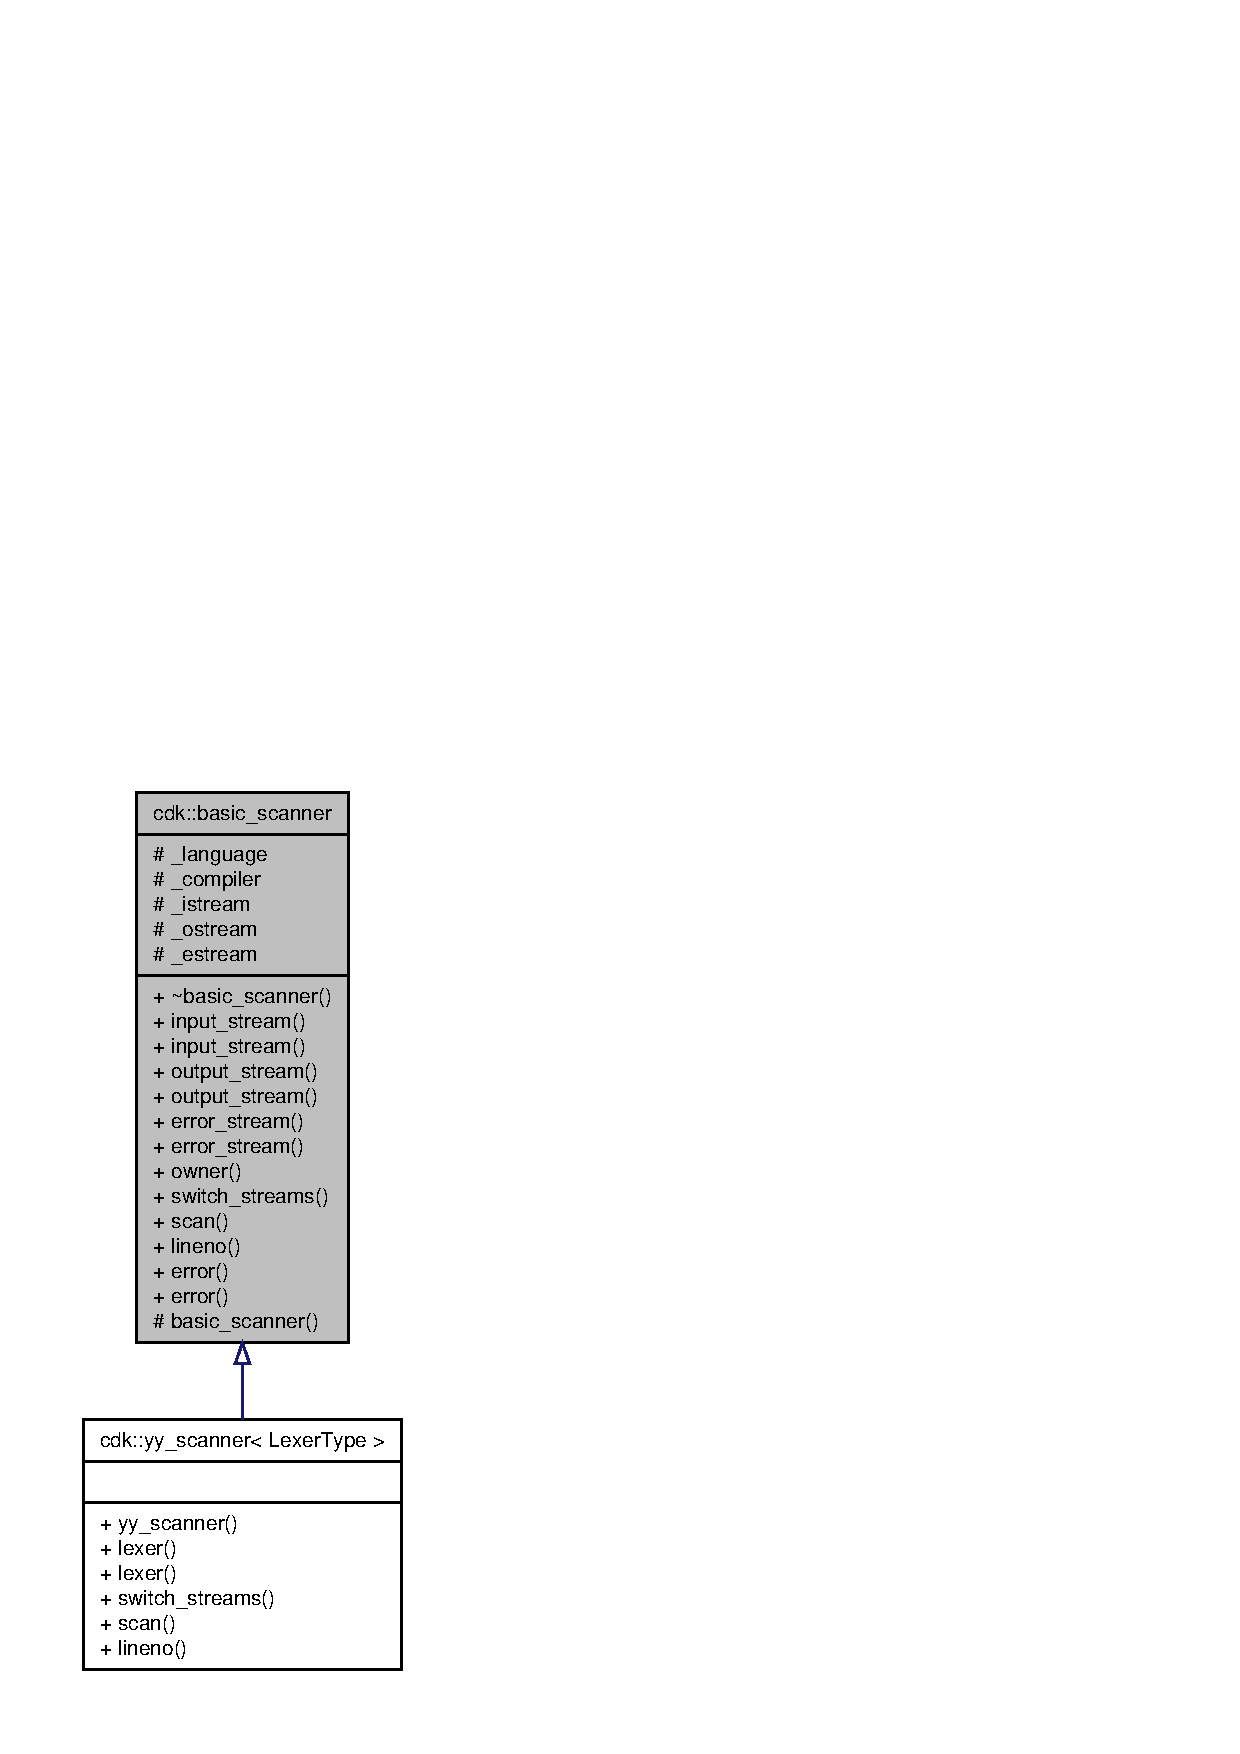
\includegraphics[width=197pt]{classcdk_1_1basic__scanner__inherit__graph}
\end{center}
\end{figure}


Collaboration diagram for cdk\+:\+:basic\+\_\+scanner\+:
\nopagebreak
\begin{figure}[H]
\begin{center}
\leavevmode
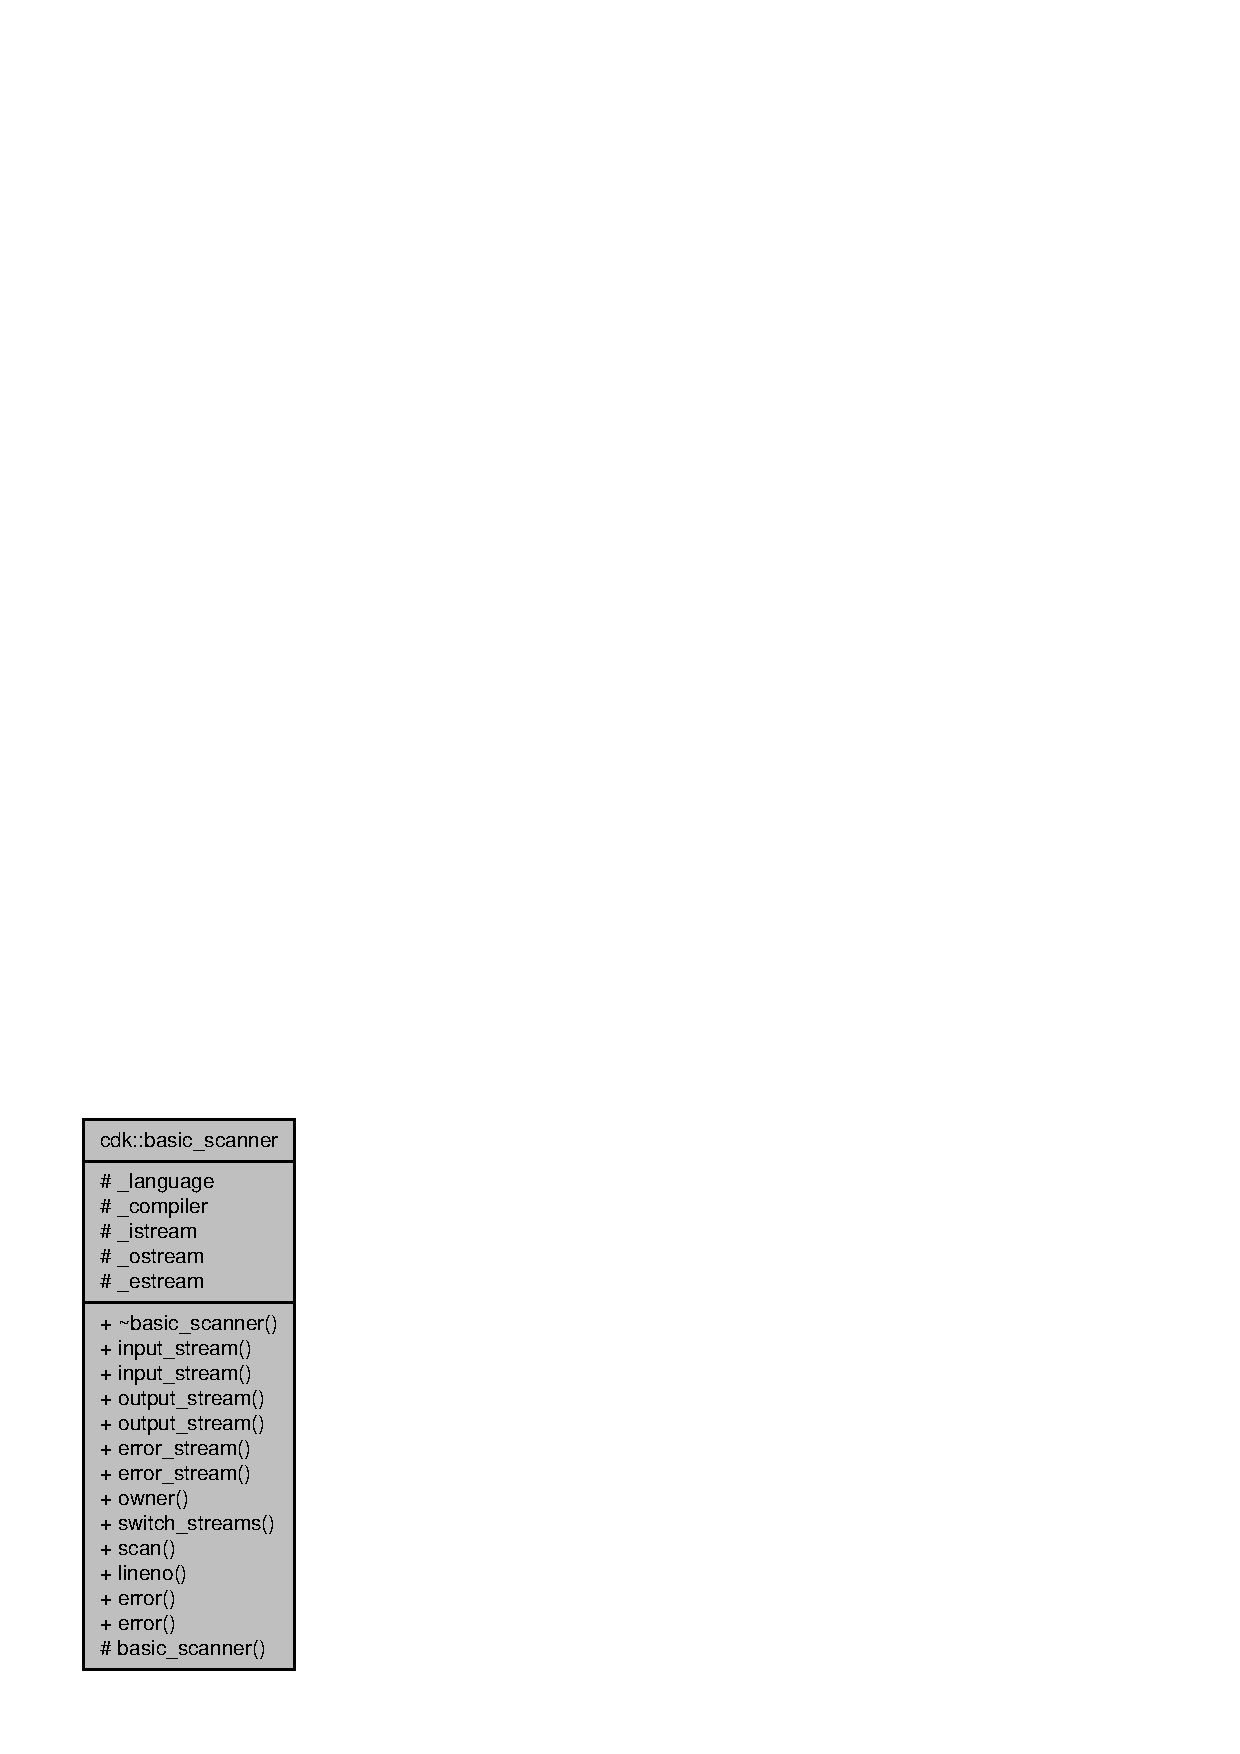
\includegraphics[width=146pt]{classcdk_1_1basic__scanner__coll__graph}
\end{center}
\end{figure}
\subsection*{Public Member Functions}
\begin{DoxyCompactItemize}
\item 
\mbox{\label{classcdk_1_1basic__scanner_a84724c88be29e36456e3d91a4e6408e9}} 
virtual \textbf{ $\sim$basic\+\_\+scanner} ()
\begin{DoxyCompactList}\small\item\em How to destroy a scanner. \end{DoxyCompactList}\item 
\mbox{\label{classcdk_1_1basic__scanner_a1844bebafdea3dddd4533e37c9c493f0}} 
std\+::shared\+\_\+ptr$<$ std\+::istream $>$ {\bfseries input\+\_\+stream} ()
\item 
\mbox{\label{classcdk_1_1basic__scanner_a9c6dd4e6d2d776e670cde1c5801cb8c4}} 
void {\bfseries input\+\_\+stream} (std\+::shared\+\_\+ptr$<$ std\+::istream $>$ istr)
\item 
\mbox{\label{classcdk_1_1basic__scanner_a90349782202ffa3c4afd0368215d5c74}} 
std\+::shared\+\_\+ptr$<$ std\+::ostream $>$ {\bfseries output\+\_\+stream} ()
\item 
\mbox{\label{classcdk_1_1basic__scanner_af48b0fdaef91f8620fd8307a7bcce21f}} 
void {\bfseries output\+\_\+stream} (std\+::shared\+\_\+ptr$<$ std\+::ostream $>$ ostr)
\item 
\mbox{\label{classcdk_1_1basic__scanner_a7b915ebc3e30a39b98358fa0ab9e291e}} 
std\+::shared\+\_\+ptr$<$ std\+::ostream $>$ {\bfseries error\+\_\+stream} ()
\item 
\mbox{\label{classcdk_1_1basic__scanner_a1907b7d54ba7b569a46abe427ef3c72e}} 
void {\bfseries error\+\_\+stream} (std\+::shared\+\_\+ptr$<$ std\+::ostream $>$ estr)
\item 
\mbox{\label{classcdk_1_1basic__scanner_a5997574b9ef358ae140995d2b455146a}} 
std\+::shared\+\_\+ptr$<$ \textbf{ compiler} $>$ {\bfseries owner} ()
\item 
\mbox{\label{classcdk_1_1basic__scanner_a945cd1fe3044cd563a21b5821f607a4e}} 
virtual void {\bfseries switch\+\_\+streams} ()=0
\item 
virtual int \textbf{ scan} ()=0
\item 
virtual int \textbf{ lineno} () const =0
\item 
virtual void \textbf{ error} (const std\+::string \&message) const
\item 
virtual void \textbf{ error} (const char $\ast$const message) const
\end{DoxyCompactItemize}
\subsection*{Protected Member Functions}
\begin{DoxyCompactItemize}
\item 
\mbox{\label{classcdk_1_1basic__scanner_a2248aa3bdf1cbbd99791c082c0ff0622}} 
{\bfseries basic\+\_\+scanner} (const std\+::string \&language)
\end{DoxyCompactItemize}
\subsection*{Protected Attributes}
\begin{DoxyCompactItemize}
\item 
\mbox{\label{classcdk_1_1basic__scanner_a5df3f99fae0e4d32f37a7c866b5a49f9}} 
const std\+::string {\bfseries \+\_\+language} = \char`\"{}\char`\"{}
\item 
\mbox{\label{classcdk_1_1basic__scanner_adacdfd18dfe6318bbcf10d164e491a90}} 
std\+::shared\+\_\+ptr$<$ \textbf{ compiler} $>$ {\bfseries \+\_\+compiler} = nullptr
\item 
std\+::shared\+\_\+ptr$<$ std\+::istream $>$ {\bfseries \+\_\+istream}
\item 
std\+::shared\+\_\+ptr$<$ std\+::ostream $>$ {\bfseries \+\_\+ostream}
\item 
std\+::shared\+\_\+ptr$<$ std\+::ostream $>$ {\bfseries \+\_\+estream}
\end{DoxyCompactItemize}
\subsection*{Friends}
\begin{DoxyCompactItemize}
\item 
\mbox{\label{classcdk_1_1basic__scanner_a0cda9b397092fcd36f20439c161a8f79}} 
class {\bfseries basic\+\_\+parser}
\item 
\mbox{\label{classcdk_1_1basic__scanner_a6450bc9182feebc4fe52fbf86fa0ba40}} 
class {\bfseries compiler}
\end{DoxyCompactItemize}


\subsection{Detailed Description}


Definition at line 14 of file basic\+\_\+scanner.\+h.



\subsection{Member Function Documentation}
\mbox{\label{classcdk_1_1basic__scanner_ac143930ad276ca56f586211fc52d61f2}} 
\index{cdk\+::basic\+\_\+scanner@{cdk\+::basic\+\_\+scanner}!error@{error}}
\index{error@{error}!cdk\+::basic\+\_\+scanner@{cdk\+::basic\+\_\+scanner}}
\subsubsection{error()\hspace{0.1cm}{\footnotesize\ttfamily [1/2]}}
{\footnotesize\ttfamily virtual void cdk\+::basic\+\_\+scanner\+::error (\begin{DoxyParamCaption}\item[{const std\+::string \&}]{message }\end{DoxyParamCaption}) const\hspace{0.3cm}{\ttfamily [inline]}, {\ttfamily [virtual]}}

Output error message. 

Definition at line 109 of file basic\+\_\+scanner.\+h.



References lineno().

Here is the call graph for this function\+:
\nopagebreak
\begin{figure}[H]
\begin{center}
\leavevmode
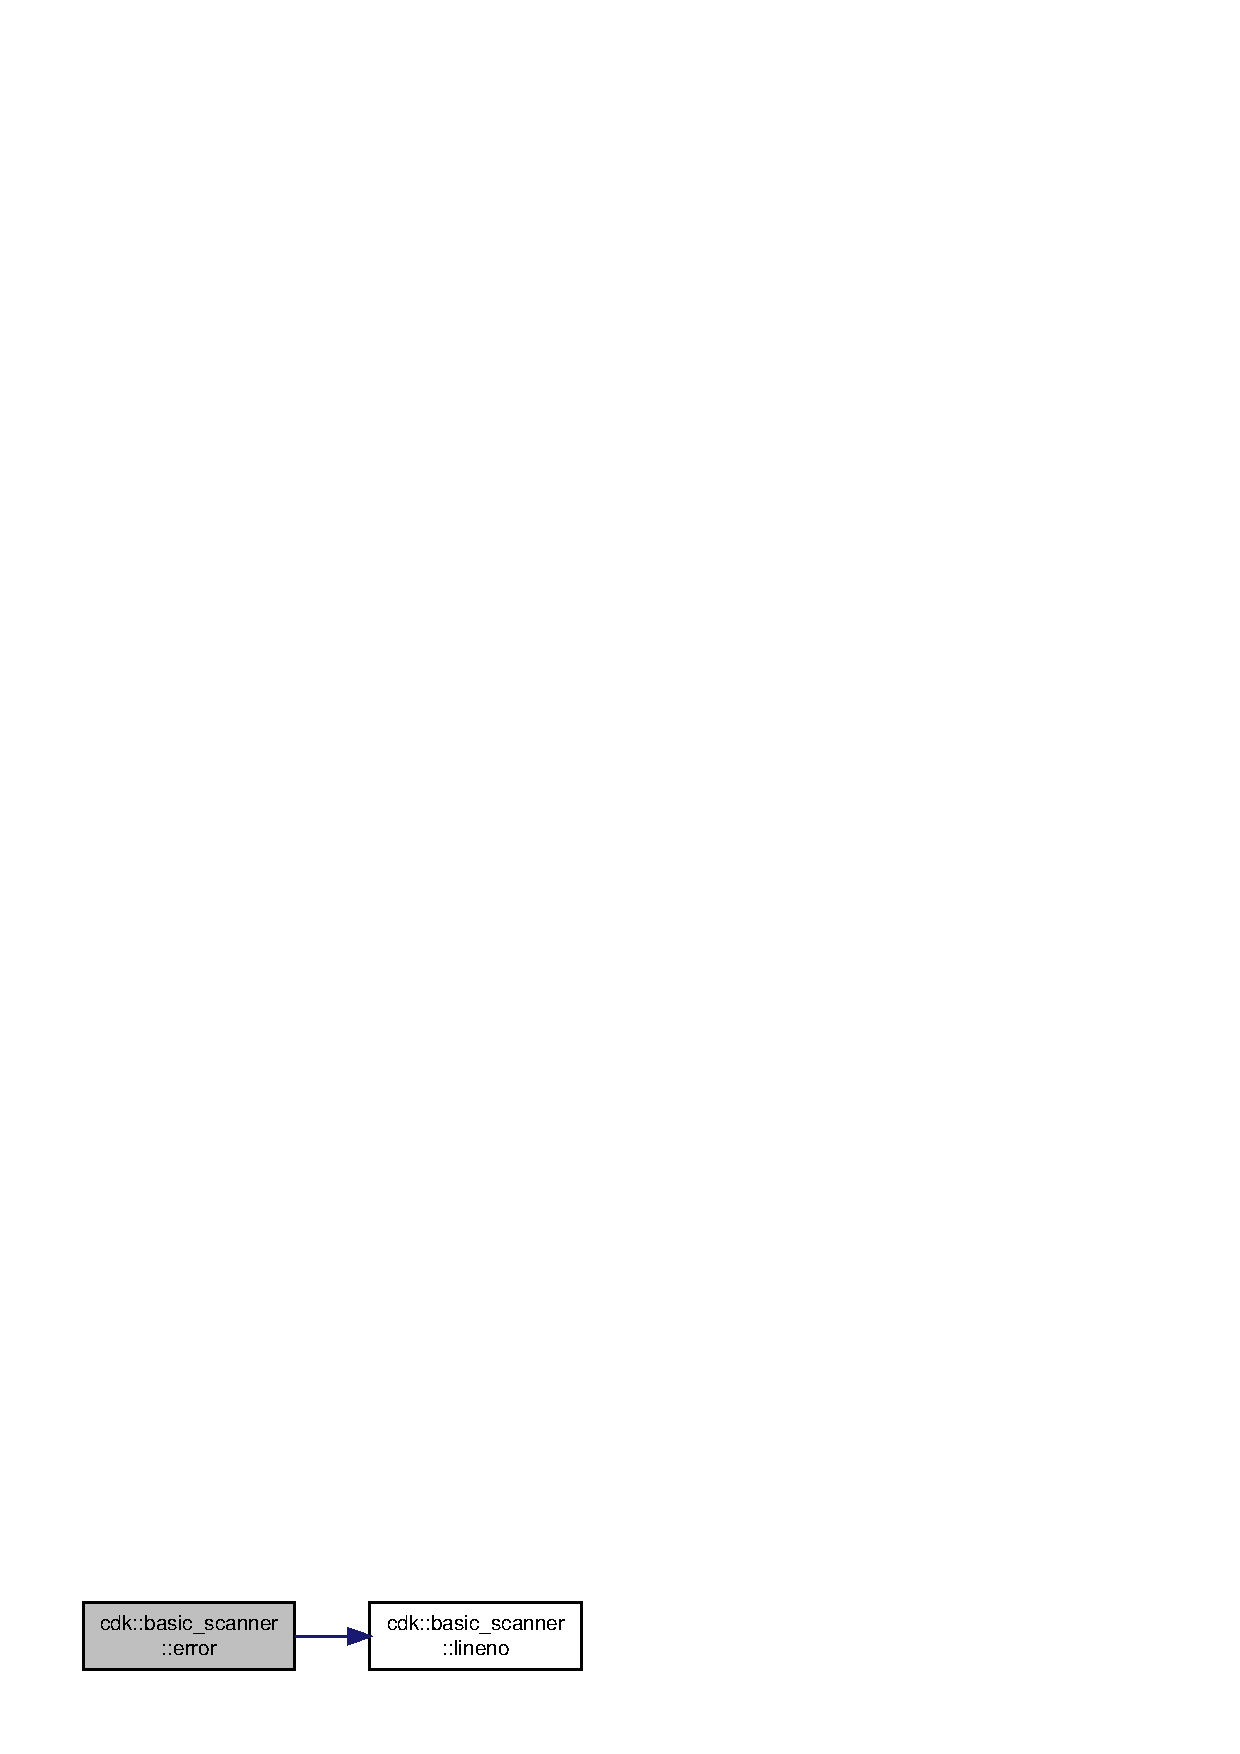
\includegraphics[width=283pt]{classcdk_1_1basic__scanner_ac143930ad276ca56f586211fc52d61f2_cgraph}
\end{center}
\end{figure}
\mbox{\label{classcdk_1_1basic__scanner_a580a8c7525cd0fabe815afbb6c071c0c}} 
\index{cdk\+::basic\+\_\+scanner@{cdk\+::basic\+\_\+scanner}!error@{error}}
\index{error@{error}!cdk\+::basic\+\_\+scanner@{cdk\+::basic\+\_\+scanner}}
\subsubsection{error()\hspace{0.1cm}{\footnotesize\ttfamily [2/2]}}
{\footnotesize\ttfamily virtual void cdk\+::basic\+\_\+scanner\+::error (\begin{DoxyParamCaption}\item[{const char $\ast$const}]{message }\end{DoxyParamCaption}) const\hspace{0.3cm}{\ttfamily [inline]}, {\ttfamily [virtual]}}

Output error message. 

Definition at line 116 of file basic\+\_\+scanner.\+h.



References lineno().

Here is the call graph for this function\+:
\nopagebreak
\begin{figure}[H]
\begin{center}
\leavevmode
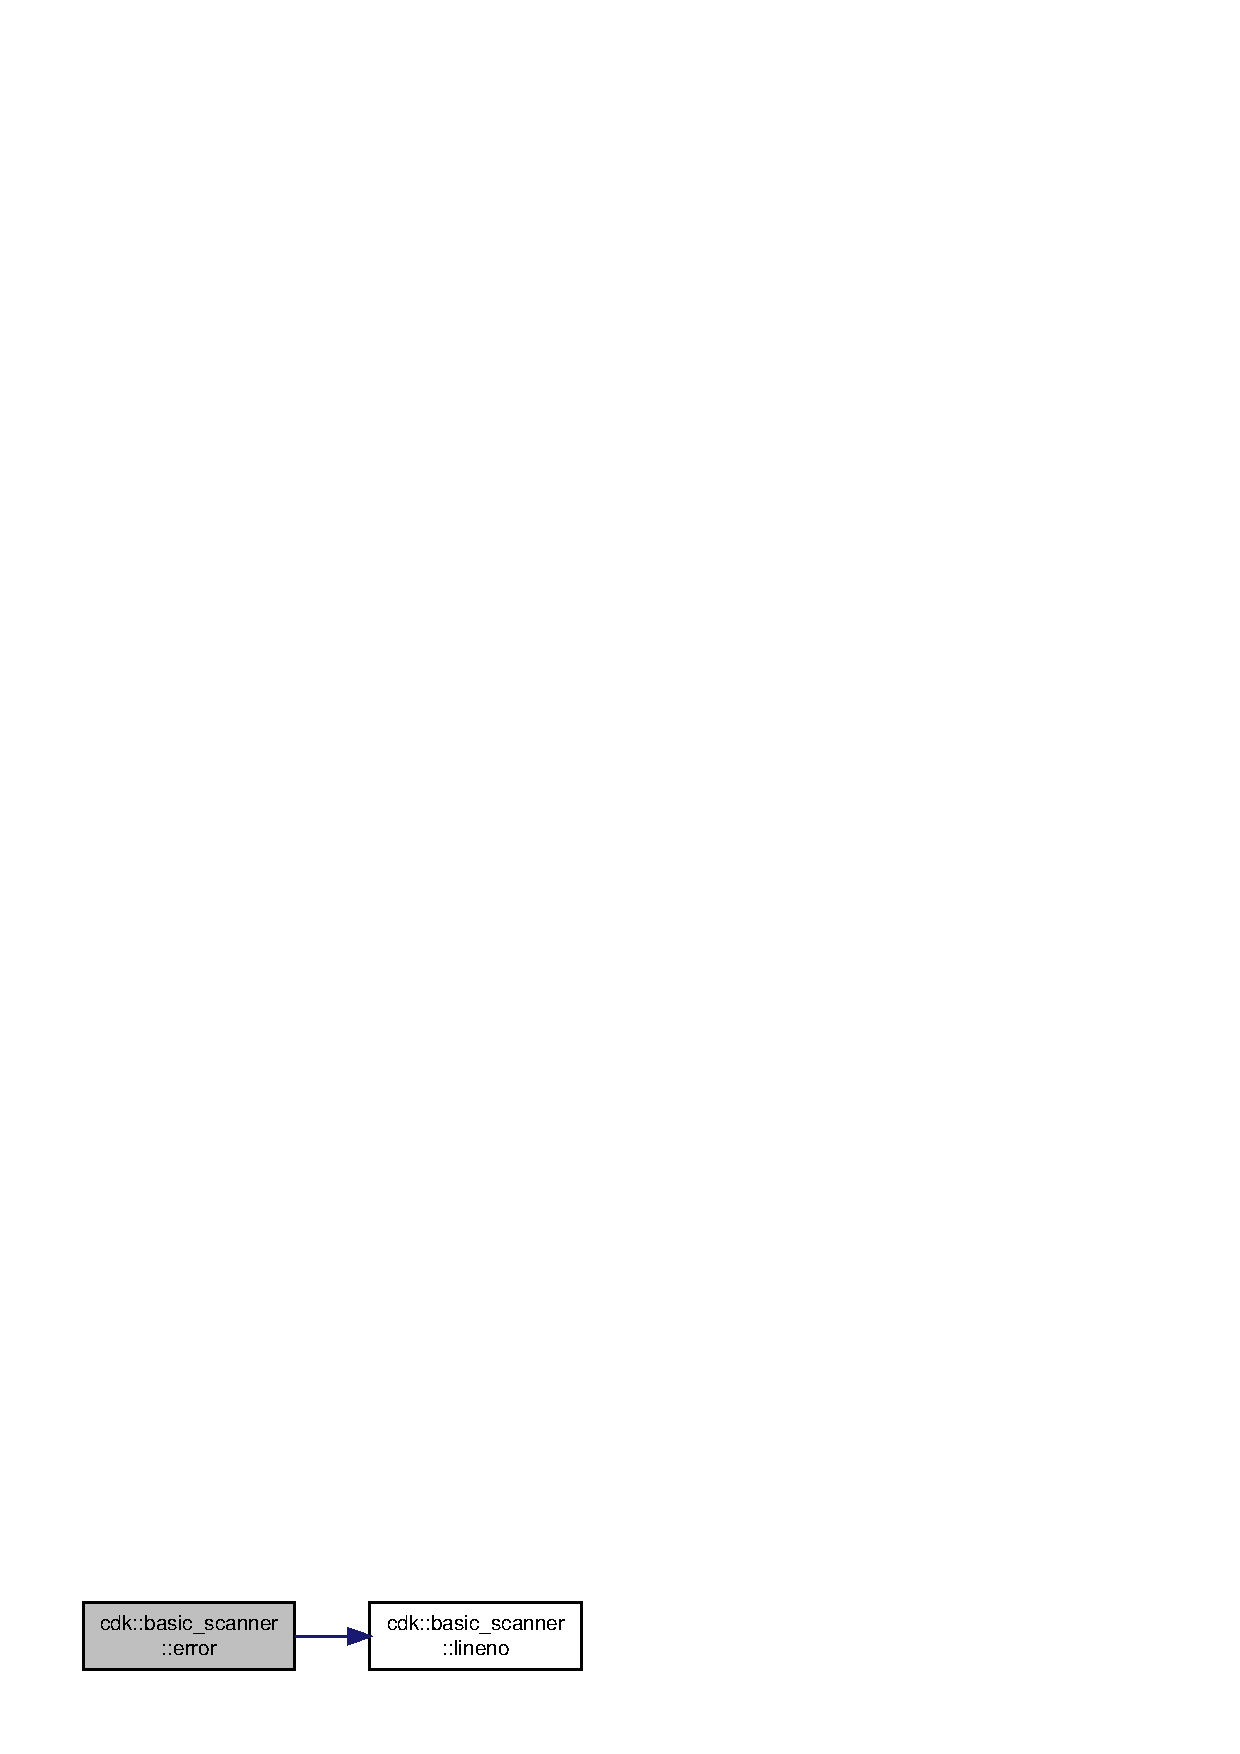
\includegraphics[width=283pt]{classcdk_1_1basic__scanner_a580a8c7525cd0fabe815afbb6c071c0c_cgraph}
\end{center}
\end{figure}
\mbox{\label{classcdk_1_1basic__scanner_a958d6207e97b29606410fba4204a60db}} 
\index{cdk\+::basic\+\_\+scanner@{cdk\+::basic\+\_\+scanner}!lineno@{lineno}}
\index{lineno@{lineno}!cdk\+::basic\+\_\+scanner@{cdk\+::basic\+\_\+scanner}}
\subsubsection{lineno()}
{\footnotesize\ttfamily virtual int cdk\+::basic\+\_\+scanner\+::lineno (\begin{DoxyParamCaption}{ }\end{DoxyParamCaption}) const\hspace{0.3cm}{\ttfamily [pure virtual]}}

Return current source line. 

Implemented in \textbf{ cdk\+::yy\+\_\+scanner$<$ Lexer\+Type $>$} \doxyref{}{p.}{classcdk_1_1yy__scanner_a7dad207713b63d89bc6b0d4f88313bf3}.



Referenced by error().

\mbox{\label{classcdk_1_1basic__scanner_aad8bc66ab0e2247392a91057b1bd55cf}} 
\index{cdk\+::basic\+\_\+scanner@{cdk\+::basic\+\_\+scanner}!scan@{scan}}
\index{scan@{scan}!cdk\+::basic\+\_\+scanner@{cdk\+::basic\+\_\+scanner}}
\subsubsection{scan()}
{\footnotesize\ttfamily virtual int cdk\+::basic\+\_\+scanner\+::scan (\begin{DoxyParamCaption}{ }\end{DoxyParamCaption})\hspace{0.3cm}{\ttfamily [pure virtual]}}

Scanning algorithm\+: the compiler object stores the result. 
\begin{DoxyParams}{Parameters}
{\em compiler} & the compiler object this parser belongs to. \\
\hline
\end{DoxyParams}
\begin{DoxyReturn}{Returns}
true if the operation is successful 
\end{DoxyReturn}


Implemented in \textbf{ cdk\+::yy\+\_\+scanner$<$ Lexer\+Type $>$} \doxyref{}{p.}{classcdk_1_1yy__scanner_af3a3f2fc181718ef27ea44870474e3ec}.



\subsection{Member Data Documentation}
\mbox{\label{classcdk_1_1basic__scanner_ac0c7edce1f9288b2cc5a93087807879c}} 
\index{cdk\+::basic\+\_\+scanner@{cdk\+::basic\+\_\+scanner}!\+\_\+estream@{\+\_\+estream}}
\index{\+\_\+estream@{\+\_\+estream}!cdk\+::basic\+\_\+scanner@{cdk\+::basic\+\_\+scanner}}
\subsubsection{\+\_\+estream}
{\footnotesize\ttfamily std\+::shared\+\_\+ptr$<$std\+::ostream$>$ cdk\+::basic\+\_\+scanner\+::\+\_\+estream\hspace{0.3cm}{\ttfamily [protected]}}

{\bfseries Initial value\+:}
\begin{DoxyCode}
= std::shared\_ptr<std::ostream>(&std::cerr,
                                                                           null\_deleter())
\end{DoxyCode}


Definition at line 36 of file basic\+\_\+scanner.\+h.

\mbox{\label{classcdk_1_1basic__scanner_af1c1bc5c903b5335ad6d4ddd28ea1c65}} 
\index{cdk\+::basic\+\_\+scanner@{cdk\+::basic\+\_\+scanner}!\+\_\+istream@{\+\_\+istream}}
\index{\+\_\+istream@{\+\_\+istream}!cdk\+::basic\+\_\+scanner@{cdk\+::basic\+\_\+scanner}}
\subsubsection{\+\_\+istream}
{\footnotesize\ttfamily std\+::shared\+\_\+ptr$<$std\+::istream$>$ cdk\+::basic\+\_\+scanner\+::\+\_\+istream\hspace{0.3cm}{\ttfamily [protected]}}

{\bfseries Initial value\+:}
\begin{DoxyCode}
= std::shared\_ptr<std::istream>(&std::cin,
                                                                           null\_deleter())
\end{DoxyCode}


Definition at line 28 of file basic\+\_\+scanner.\+h.

\mbox{\label{classcdk_1_1basic__scanner_a4a1e22ea48e5cbe116e68f99b7463096}} 
\index{cdk\+::basic\+\_\+scanner@{cdk\+::basic\+\_\+scanner}!\+\_\+ostream@{\+\_\+ostream}}
\index{\+\_\+ostream@{\+\_\+ostream}!cdk\+::basic\+\_\+scanner@{cdk\+::basic\+\_\+scanner}}
\subsubsection{\+\_\+ostream}
{\footnotesize\ttfamily std\+::shared\+\_\+ptr$<$std\+::ostream$>$ cdk\+::basic\+\_\+scanner\+::\+\_\+ostream\hspace{0.3cm}{\ttfamily [protected]}}

{\bfseries Initial value\+:}
\begin{DoxyCode}
= std::shared\_ptr<std::ostream>(&std::cout,
                                                                           null\_deleter())
\end{DoxyCode}


Definition at line 32 of file basic\+\_\+scanner.\+h.



The documentation for this class was generated from the following file\+:\begin{DoxyCompactItemize}
\item 
basic\+\_\+scanner.\+h\end{DoxyCompactItemize}

\section{cdk\+:\+:basic\+\_\+target Class Reference}
\label{classcdk_1_1basic__target}\index{cdk\+::basic\+\_\+target@{cdk\+::basic\+\_\+target}}


Collaboration diagram for cdk\+:\+:basic\+\_\+target\+:
\nopagebreak
\begin{figure}[H]
\begin{center}
\leavevmode
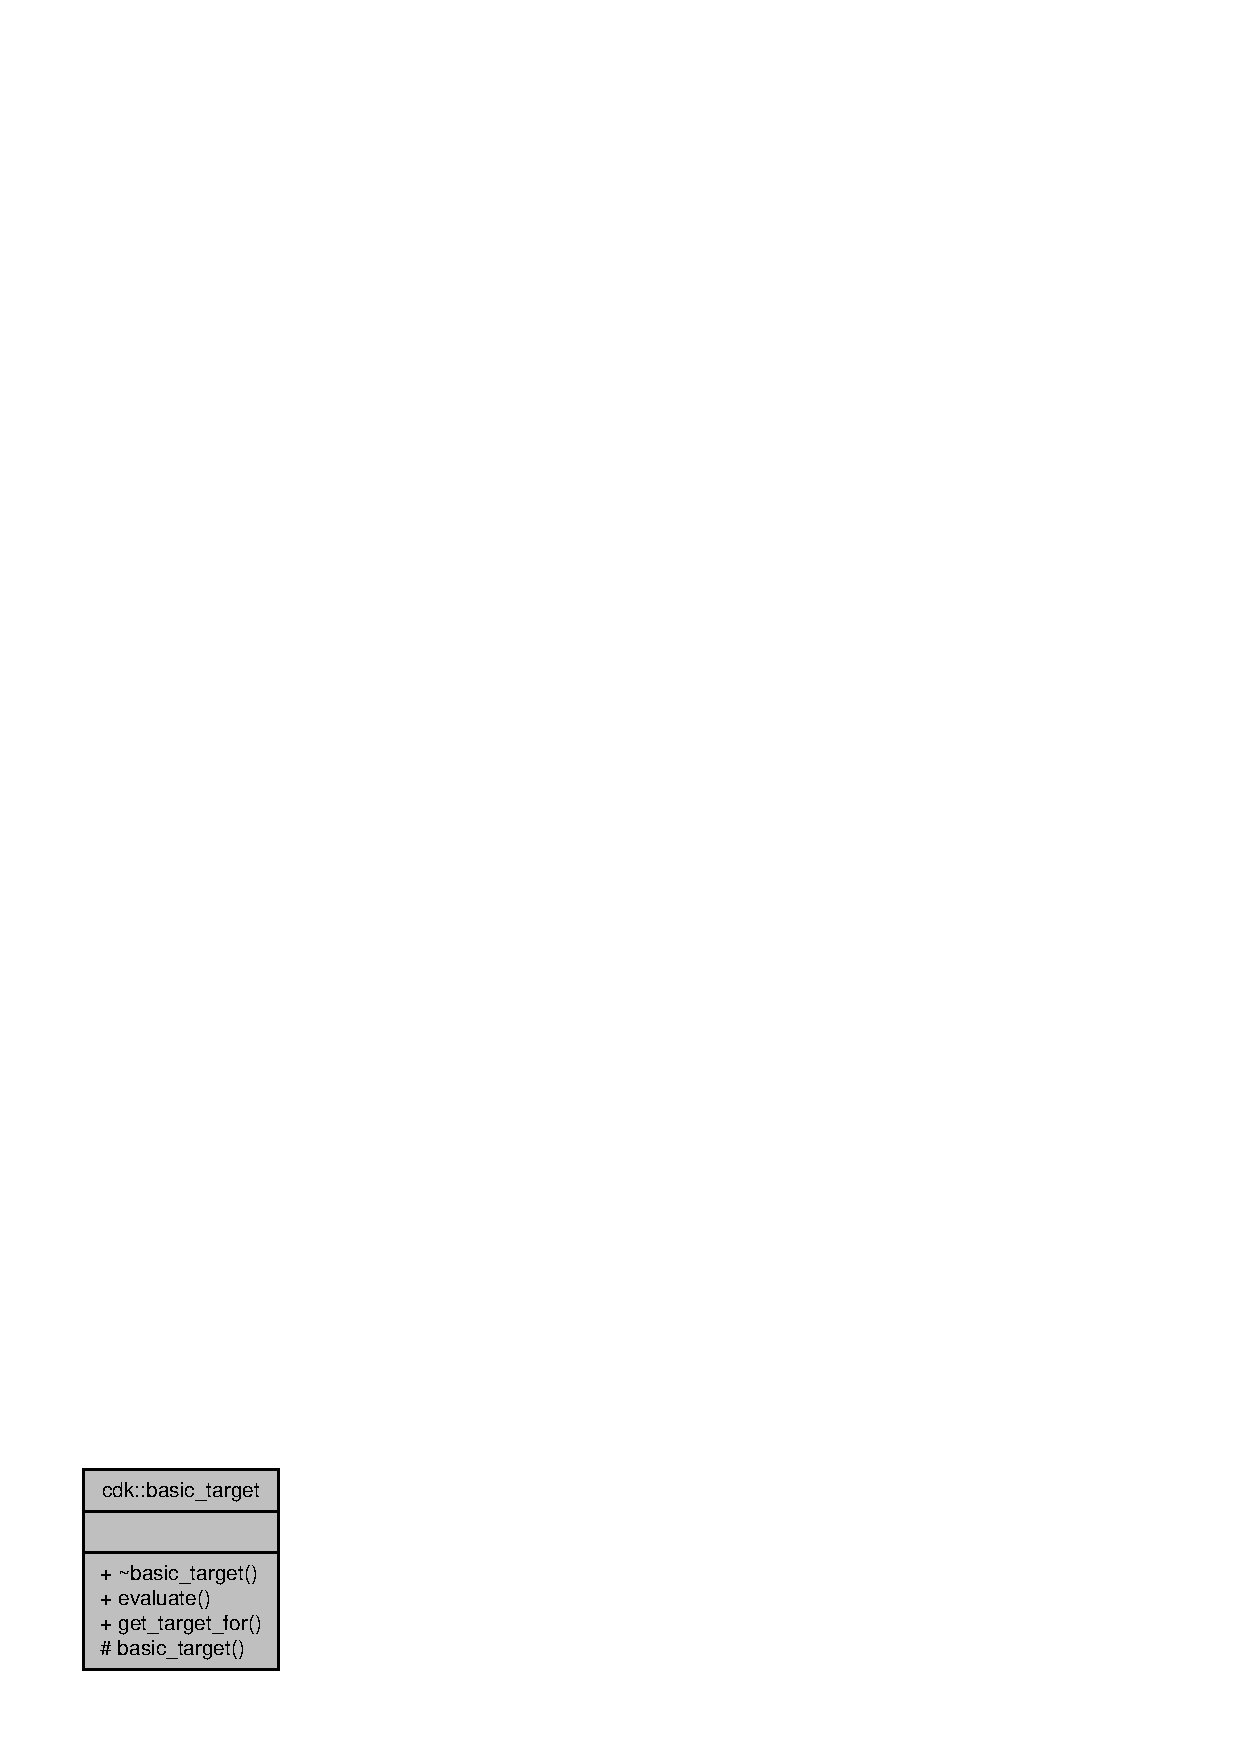
\includegraphics[width=138pt]{classcdk_1_1basic__target__coll__graph}
\end{center}
\end{figure}
\subsection*{Public Member Functions}
\begin{DoxyCompactItemize}
\item 
\mbox{\label{classcdk_1_1basic__target_aaa74cb39cf10b2735b1abc15680898fa}} 
virtual \textbf{ $\sim$basic\+\_\+target} ()
\begin{DoxyCompactList}\small\item\em How to destroy an evaluator. \end{DoxyCompactList}\item 
virtual bool \textbf{ evaluate} (std\+::shared\+\_\+ptr$<$ \textbf{ compiler} $>$)=0
\end{DoxyCompactItemize}
\subsection*{Static Public Member Functions}
\begin{DoxyCompactItemize}
\item 
static \textbf{ basic\+\_\+target} $\ast$ \textbf{ get\+\_\+target\+\_\+for} (const std\+::string \&target)
\end{DoxyCompactItemize}
\subsection*{Protected Member Functions}
\begin{DoxyCompactItemize}
\item 
\mbox{\label{classcdk_1_1basic__target_a789431eed534e3827eb2686ed00f30b8}} 
{\bfseries basic\+\_\+target} (const char $\ast$target)
\end{DoxyCompactItemize}


\subsection{Detailed Description}


Definition at line 15 of file basic\+\_\+target.\+h.



\subsection{Member Function Documentation}
\mbox{\label{classcdk_1_1basic__target_a0db773c9c4f84a36df0949187aab9adb}} 
\index{cdk\+::basic\+\_\+target@{cdk\+::basic\+\_\+target}!evaluate@{evaluate}}
\index{evaluate@{evaluate}!cdk\+::basic\+\_\+target@{cdk\+::basic\+\_\+target}}
\subsubsection{evaluate()}
{\footnotesize\ttfamily virtual bool cdk\+::basic\+\_\+target\+::evaluate (\begin{DoxyParamCaption}\item[{std\+::shared\+\_\+ptr$<$ \textbf{ compiler} $>$}]{ }\end{DoxyParamCaption})\hspace{0.3cm}{\ttfamily [pure virtual]}}

Evaluation algorithm for a syntax tree\+: processes the tree and sends the result to the output stream. 
\begin{DoxyParams}{Parameters}
{\em compiler} & object representing the compiler as a whole \\
\hline
\end{DoxyParams}
\begin{DoxyReturn}{Returns}
true if the operation is successful 
\end{DoxyReturn}


Referenced by cdk\+::compiler\+::evaluate().

\mbox{\label{classcdk_1_1basic__target_a50126c8601a5b82dcce46e43d4258064}} 
\index{cdk\+::basic\+\_\+target@{cdk\+::basic\+\_\+target}!get\+\_\+target\+\_\+for@{get\+\_\+target\+\_\+for}}
\index{get\+\_\+target\+\_\+for@{get\+\_\+target\+\_\+for}!cdk\+::basic\+\_\+target@{cdk\+::basic\+\_\+target}}
\subsubsection{get\+\_\+target\+\_\+for()}
{\footnotesize\ttfamily static \textbf{ basic\+\_\+target}$\ast$ cdk\+::basic\+\_\+target\+::get\+\_\+target\+\_\+for (\begin{DoxyParamCaption}\item[{const std\+::string \&}]{target }\end{DoxyParamCaption})\hspace{0.3cm}{\ttfamily [inline]}, {\ttfamily [static]}}

How to get an evaluator for a given target. 
\begin{DoxyParams}{Parameters}
{\em target} & the target name\+: \char`\"{}asm\char`\"{}, \char`\"{}c\char`\"{}, \char`\"{}xml\char`\"{}, etc. \\
\hline
\end{DoxyParams}
\begin{DoxyReturn}{Returns}
a pointer to the evaluator object 
\end{DoxyReturn}


Definition at line 32 of file basic\+\_\+target.\+h.



Referenced by cdk\+::compiler\+::evaluate().



The documentation for this class was generated from the following file\+:\begin{DoxyCompactItemize}
\item 
basic\+\_\+target.\+h\end{DoxyCompactItemize}

\section{basic\+\_\+type Struct Reference}
\label{structbasic__type}\index{basic\+\_\+type@{basic\+\_\+type}}


{\ttfamily \#include $<$basic\+\_\+type.\+h$>$}



Collaboration diagram for basic\+\_\+type\+:
\nopagebreak
\begin{figure}[H]
\begin{center}
\leavevmode
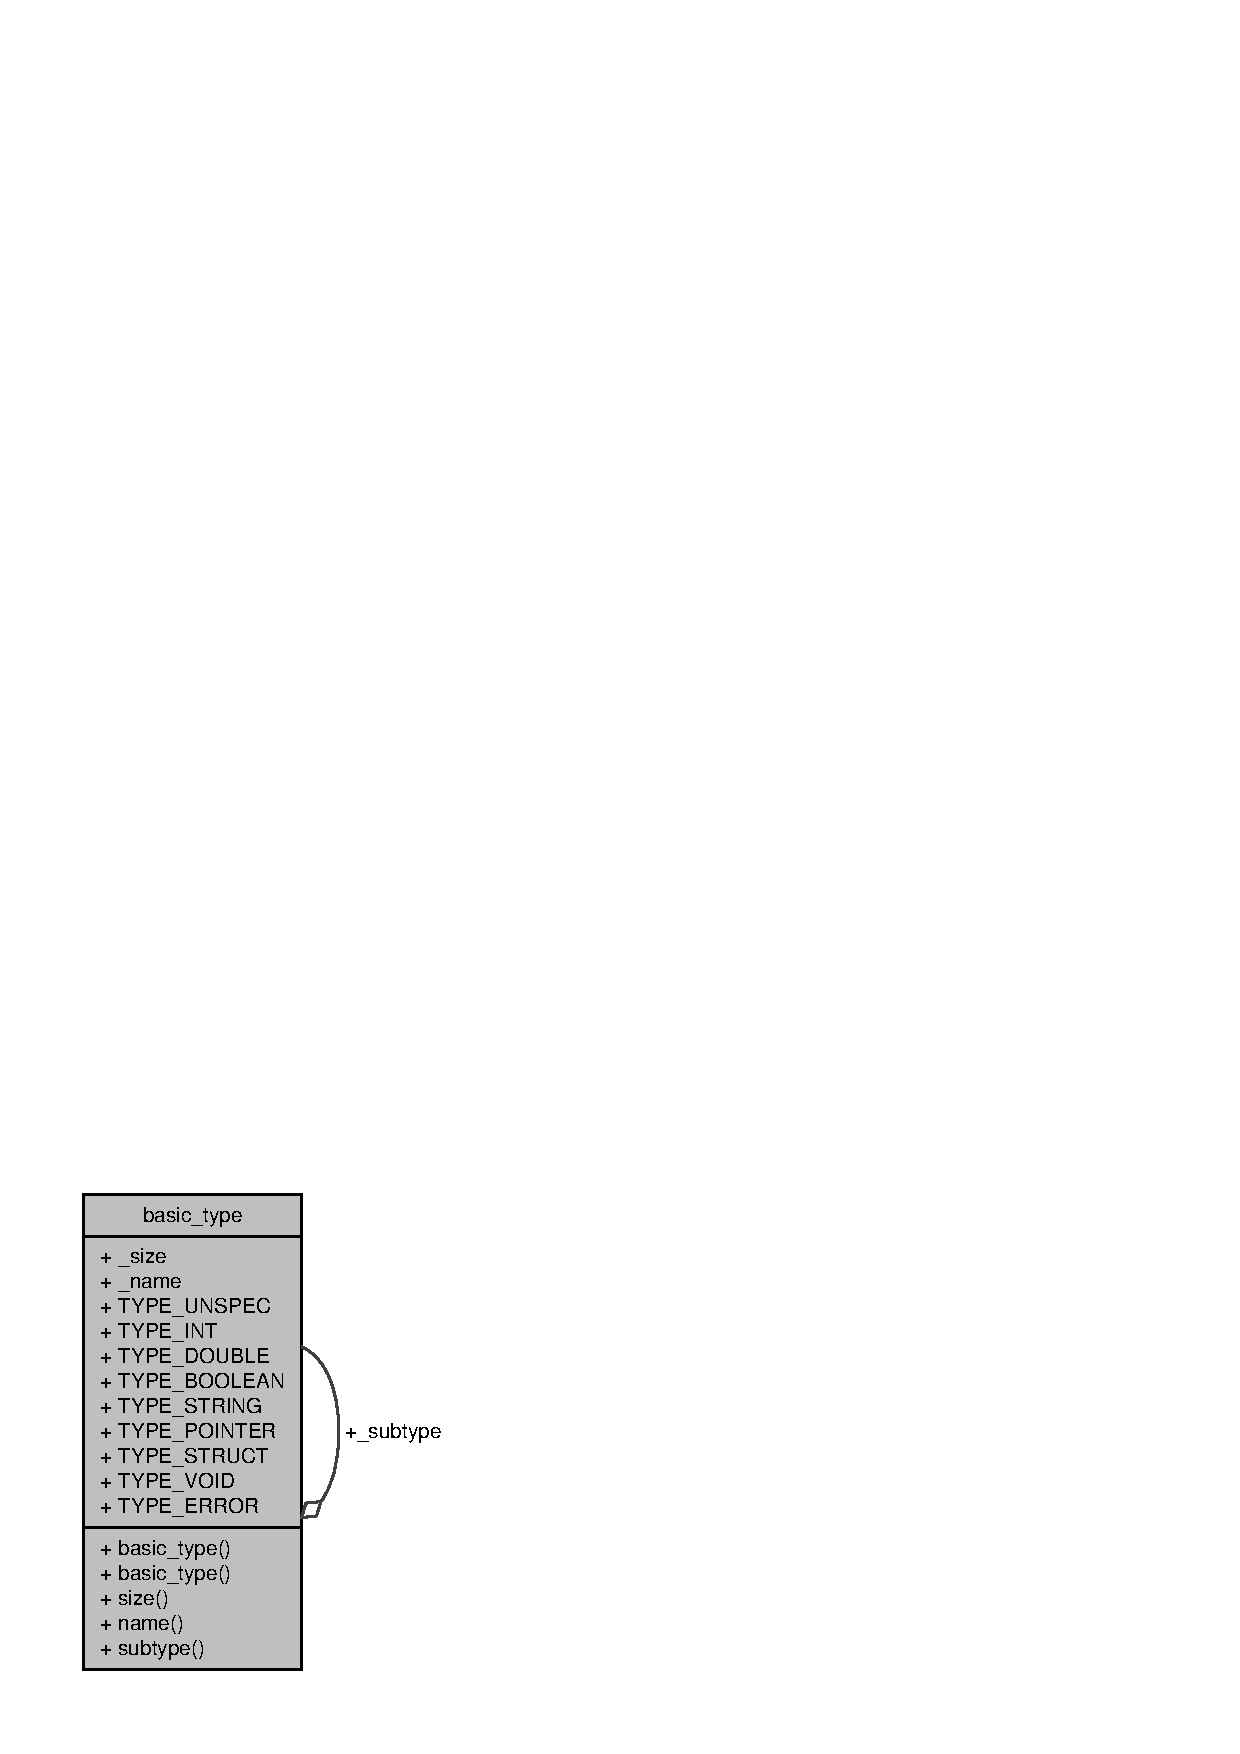
\includegraphics[width=216pt]{structbasic__type__coll__graph}
\end{center}
\end{figure}
\subsection*{Public Types}
\begin{DoxyCompactItemize}
\item 
\mbox{\label{structbasic__type_a7c0a7a590da8a3705a88d5e207e4b9ad}} 
typedef unsigned long int {\bfseries type}
\end{DoxyCompactItemize}
\subsection*{Public Member Functions}
\begin{DoxyCompactItemize}
\item 
\mbox{\label{structbasic__type_a700988000343593c00601ec255b04d0b}} 
{\bfseries basic\+\_\+type} (size\+\_\+t size, type name)
\item 
\mbox{\label{structbasic__type_a4f76b416ac41dde6d7a9f51d7e909891}} 
size\+\_\+t {\bfseries size} ()
\item 
\mbox{\label{structbasic__type_aaf747bec5153a84f07097482a77eae29}} 
type {\bfseries name} ()
\item 
\mbox{\label{structbasic__type_ac3c708c8bbd2274461227daee6b50a6a}} 
\textbf{ basic\+\_\+type} $\ast$ {\bfseries subtype} ()
\end{DoxyCompactItemize}
\subsection*{Public Attributes}
\begin{DoxyCompactItemize}
\item 
\mbox{\label{structbasic__type_a7d0e7cd683e46caea2c165fb8ebf26c5}} 
size\+\_\+t {\bfseries \+\_\+size} = 0
\item 
\mbox{\label{structbasic__type_a3fc97d3a8fc1f7ab3d037359ad705a42}} 
type {\bfseries \+\_\+name} = T\+Y\+P\+E\+\_\+\+U\+N\+S\+P\+EC
\item 
\mbox{\label{structbasic__type_a2ce9b0a06193a2bd685f106bc72a6089}} 
\textbf{ basic\+\_\+type} $\ast$ {\bfseries \+\_\+subtype} = nullptr
\end{DoxyCompactItemize}
\subsection*{Static Public Attributes}
\begin{DoxyCompactItemize}
\item 
\mbox{\label{structbasic__type_a7787995e345f10d3cc6c48d0708c8a36}} 
static const type {\bfseries T\+Y\+P\+E\+\_\+\+U\+N\+S\+P\+EC} = 0
\item 
\mbox{\label{structbasic__type_a6c904b5d042062de5ac5c454bc9426a6}} 
static const type {\bfseries T\+Y\+P\+E\+\_\+\+I\+NT} = 1\+U\+L $<$$<$ 0
\item 
\mbox{\label{structbasic__type_aa8786b1860b50978829feb20e614b4c3}} 
static const type {\bfseries T\+Y\+P\+E\+\_\+\+D\+O\+U\+B\+LE} = 1\+U\+L $<$$<$ 1
\item 
\mbox{\label{structbasic__type_a62f257e76816cc338762e6a1182174ef}} 
static const type {\bfseries T\+Y\+P\+E\+\_\+\+B\+O\+O\+L\+E\+AN} = 1\+U\+L $<$$<$ 2
\item 
\mbox{\label{structbasic__type_a2f6ab0d223597c328005e6c2276f523e}} 
static const type {\bfseries T\+Y\+P\+E\+\_\+\+S\+T\+R\+I\+NG} = 1\+U\+L $<$$<$ 3
\item 
\mbox{\label{structbasic__type_a9ded574c7b6d0a63acd29b87d8c16efe}} 
static const type {\bfseries T\+Y\+P\+E\+\_\+\+P\+O\+I\+N\+T\+ER} = 1\+U\+L $<$$<$ 4
\item 
\mbox{\label{structbasic__type_a0e3320ba9749776fbf1303d353fec55e}} 
static const type {\bfseries T\+Y\+P\+E\+\_\+\+S\+T\+R\+U\+CT} = 1\+U\+L $<$$<$ 5
\item 
\mbox{\label{structbasic__type_a59e3a52115cbe7ac8a43d64072bb98a3}} 
static const type {\bfseries T\+Y\+P\+E\+\_\+\+V\+O\+ID} = 1\+U\+L $<$$<$ 30
\item 
\mbox{\label{structbasic__type_af5146fc165cffff72de991842d60840c}} 
static const type {\bfseries T\+Y\+P\+E\+\_\+\+E\+R\+R\+OR} = 1\+U\+L $<$$<$ 31
\end{DoxyCompactItemize}


\subsection{Detailed Description}
This is a quick and very dirty approach to type information. It is defined this way (even though it\textquotesingle{}s not extensible at all) for simplicity.

Nevertheless, new types can be added simply by using other integer values other than the ones listed. 

Definition at line 14 of file basic\+\_\+type.\+h.



The documentation for this struct was generated from the following file\+:\begin{DoxyCompactItemize}
\item 
basic\+\_\+type.\+h\end{DoxyCompactItemize}

\section{cdk\+:\+:binary\+\_\+expression\+\_\+node Class Reference}
\label{classcdk_1_1binary__expression__node}\index{cdk\+::binary\+\_\+expression\+\_\+node@{cdk\+::binary\+\_\+expression\+\_\+node}}


{\ttfamily \#include $<$binary\+\_\+expression\+\_\+node.\+h$>$}



Inheritance diagram for cdk\+:\+:binary\+\_\+expression\+\_\+node\+:
\nopagebreak
\begin{figure}[H]
\begin{center}
\leavevmode
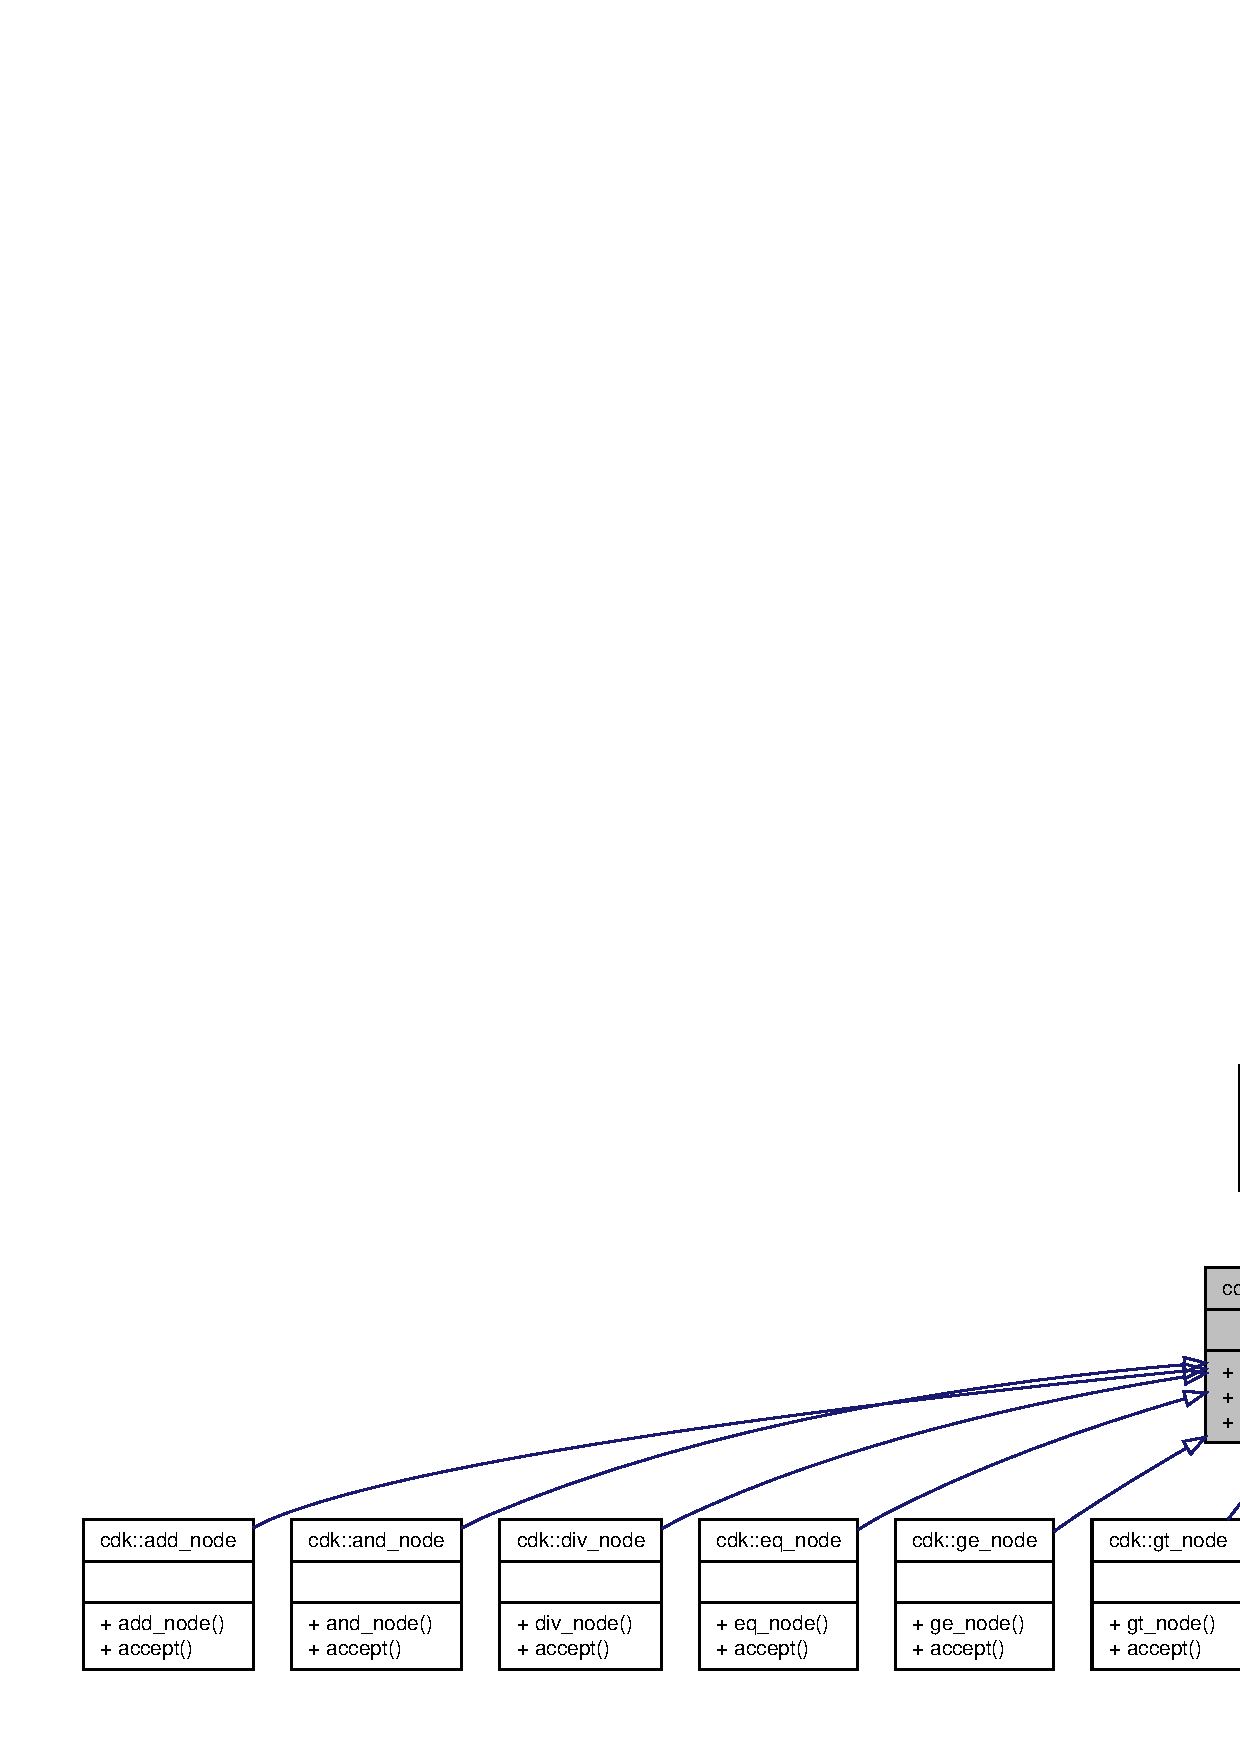
\includegraphics[width=350pt]{classcdk_1_1binary__expression__node__inherit__graph}
\end{center}
\end{figure}


Collaboration diagram for cdk\+:\+:binary\+\_\+expression\+\_\+node\+:
\nopagebreak
\begin{figure}[H]
\begin{center}
\leavevmode
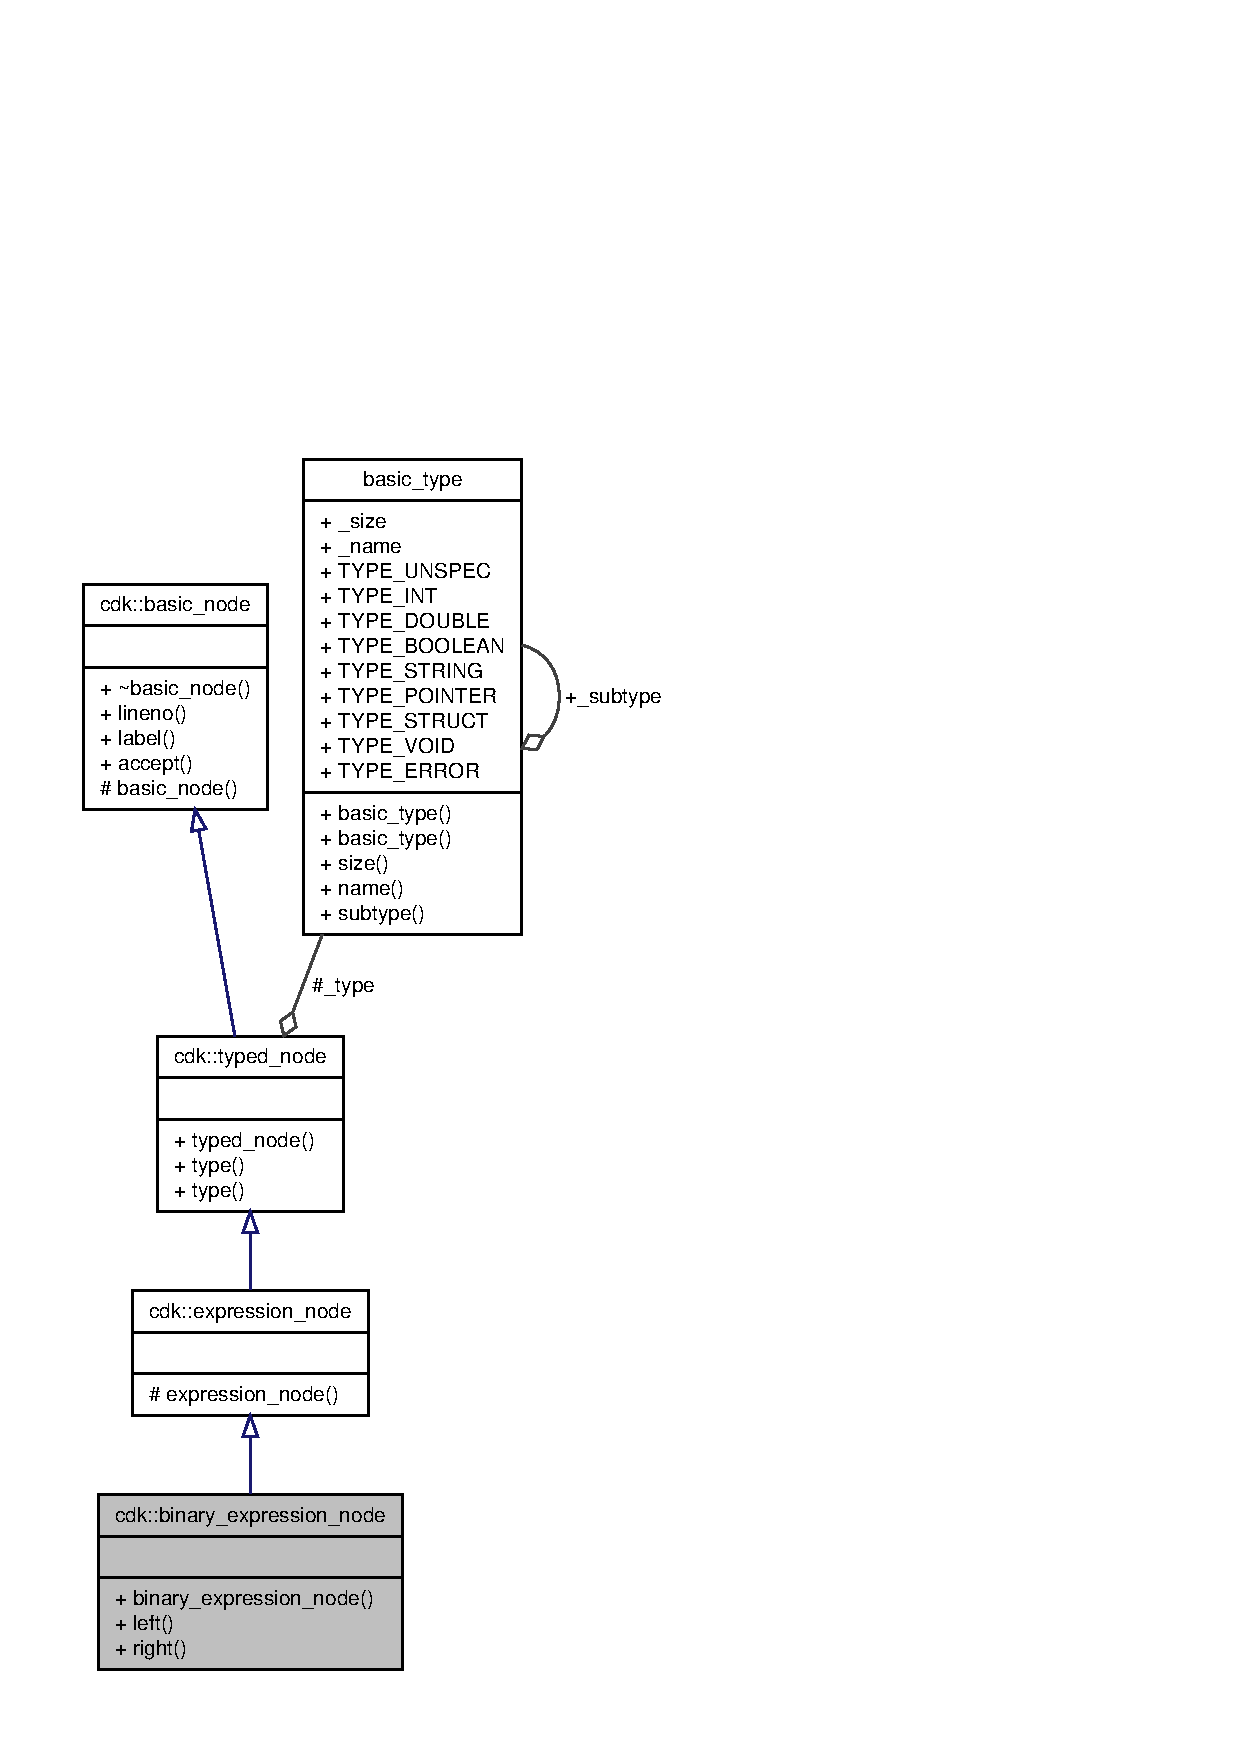
\includegraphics[height=550pt]{classcdk_1_1binary__expression__node__coll__graph}
\end{center}
\end{figure}
\subsection*{Public Member Functions}
\begin{DoxyCompactItemize}
\item 
\textbf{ binary\+\_\+expression\+\_\+node} (int \textbf{ lineno}, \textbf{ expression\+\_\+node} $\ast$left, \textbf{ expression\+\_\+node} $\ast$right)
\item 
\mbox{\label{classcdk_1_1binary__expression__node_a8ac0b884a1ea56ed16d78997066d120d}} 
\textbf{ expression\+\_\+node} $\ast$ {\bfseries left} ()
\item 
\mbox{\label{classcdk_1_1binary__expression__node_a763e869d08583a828bd1b6b5433dde52}} 
\textbf{ expression\+\_\+node} $\ast$ {\bfseries right} ()
\end{DoxyCompactItemize}
\subsection*{Additional Inherited Members}


\subsection{Detailed Description}
Class for describing binary operators. 

Definition at line 11 of file binary\+\_\+expression\+\_\+node.\+h.



\subsection{Constructor \& Destructor Documentation}
\mbox{\label{classcdk_1_1binary__expression__node_a06fa367b484369bec4645ea5274b46df}} 
\index{cdk\+::binary\+\_\+expression\+\_\+node@{cdk\+::binary\+\_\+expression\+\_\+node}!binary\+\_\+expression\+\_\+node@{binary\+\_\+expression\+\_\+node}}
\index{binary\+\_\+expression\+\_\+node@{binary\+\_\+expression\+\_\+node}!cdk\+::binary\+\_\+expression\+\_\+node@{cdk\+::binary\+\_\+expression\+\_\+node}}
\subsubsection{binary\+\_\+expression\+\_\+node()}
{\footnotesize\ttfamily cdk\+::binary\+\_\+expression\+\_\+node\+::binary\+\_\+expression\+\_\+node (\begin{DoxyParamCaption}\item[{int}]{lineno,  }\item[{\textbf{ expression\+\_\+node} $\ast$}]{left,  }\item[{\textbf{ expression\+\_\+node} $\ast$}]{right }\end{DoxyParamCaption})\hspace{0.3cm}{\ttfamily [inline]}}


\begin{DoxyParams}{Parameters}
{\em lineno} & source code line number for this node \\
\hline
{\em left} & first operand \\
\hline
{\em right} & second operand \\
\hline
\end{DoxyParams}


Definition at line 20 of file binary\+\_\+expression\+\_\+node.\+h.



The documentation for this class was generated from the following file\+:\begin{DoxyCompactItemize}
\item 
ast/binary\+\_\+expression\+\_\+node.\+h\end{DoxyCompactItemize}

\section{cdk\+:\+:compiler Class Reference}
\label{classcdk_1_1compiler}\index{cdk\+::compiler@{cdk\+::compiler}}


Inheritance diagram for cdk\+:\+:compiler\+:
\nopagebreak
\begin{figure}[H]
\begin{center}
\leavevmode
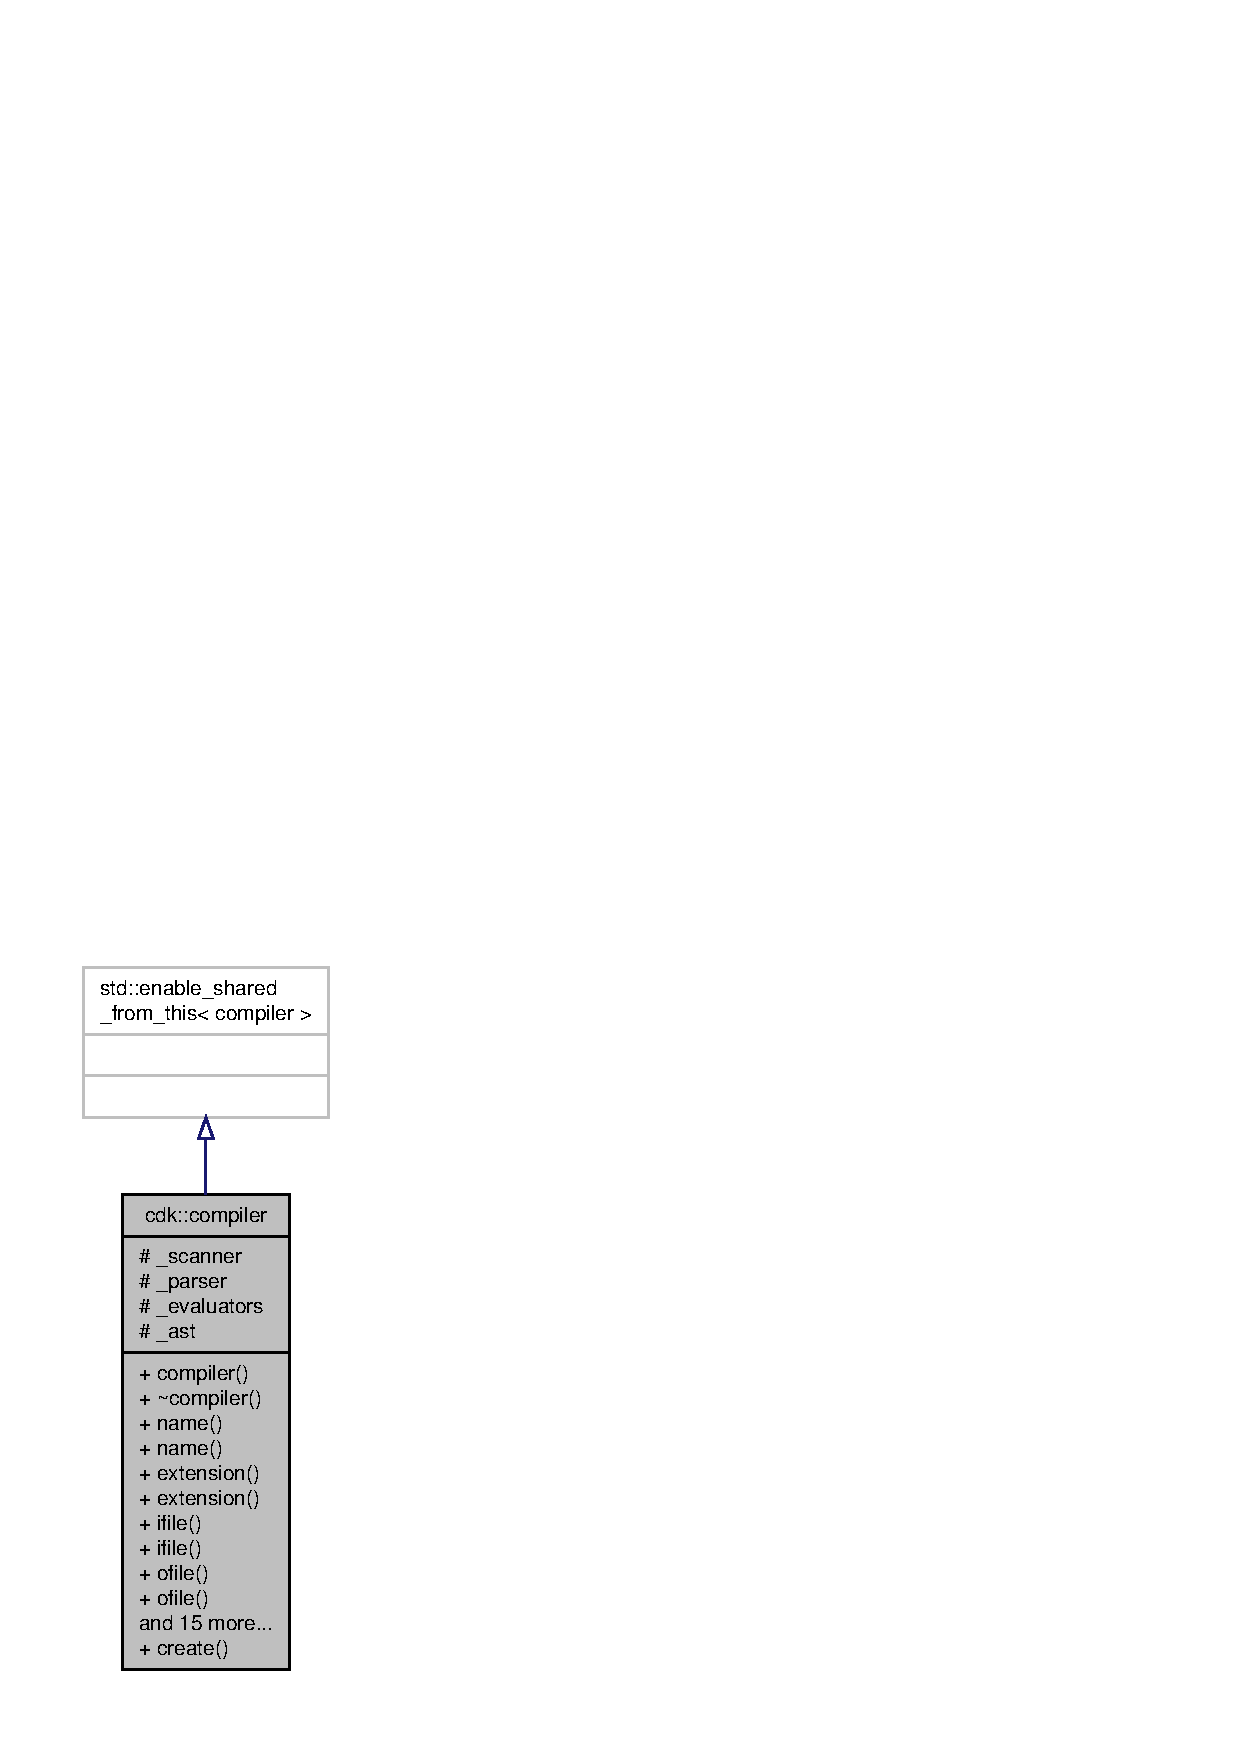
\includegraphics[width=162pt]{classcdk_1_1compiler__inherit__graph}
\end{center}
\end{figure}


Collaboration diagram for cdk\+:\+:compiler\+:
\nopagebreak
\begin{figure}[H]
\begin{center}
\leavevmode
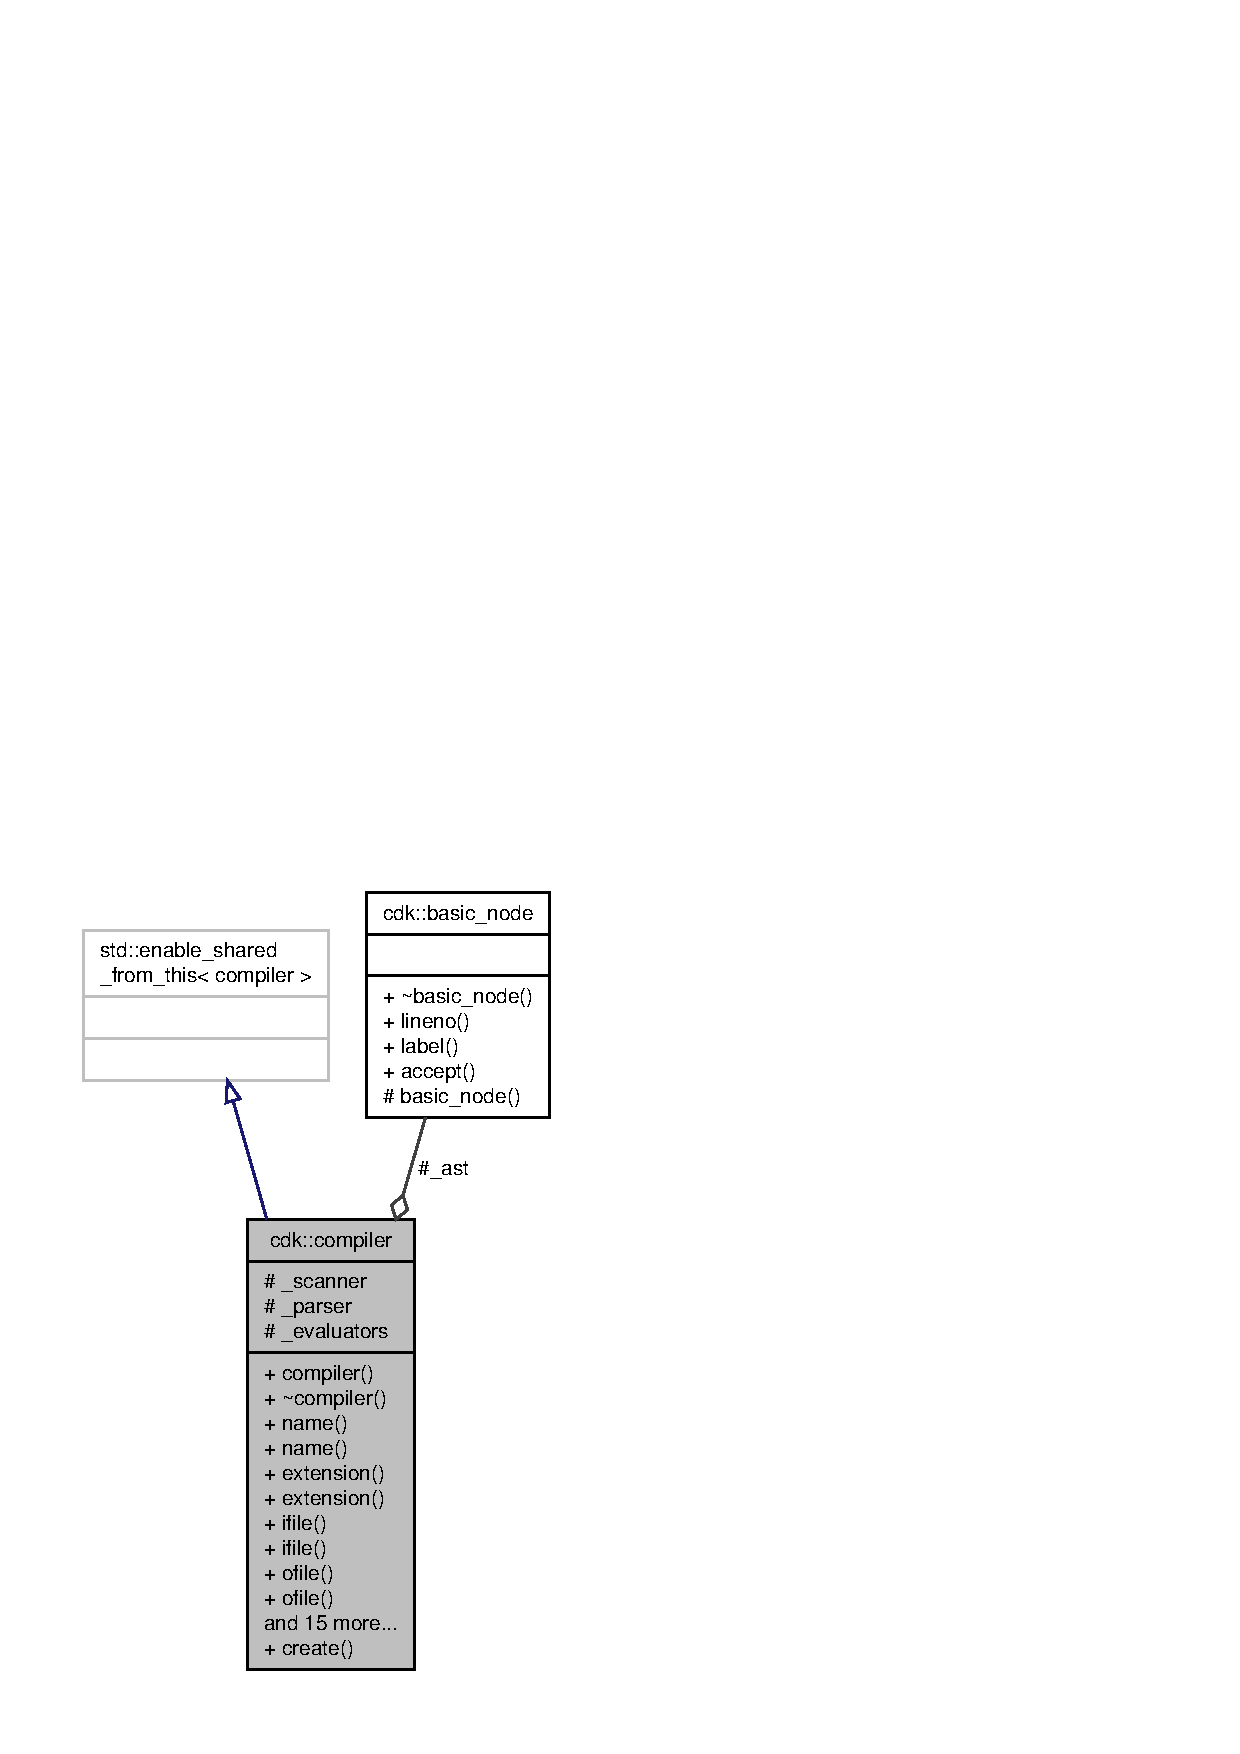
\includegraphics[width=268pt]{classcdk_1_1compiler__coll__graph}
\end{center}
\end{figure}
\subsection*{Public Member Functions}
\begin{DoxyCompactItemize}
\item 
\mbox{\label{classcdk_1_1compiler_a0718890212e30c490d31158ea8d75f73}} 
{\bfseries compiler} (const std\+::string \&language, std\+::shared\+\_\+ptr$<$ \textbf{ basic\+\_\+scanner} $>$ scanner, std\+::shared\+\_\+ptr$<$ \textbf{ basic\+\_\+parser} $>$ parser)
\item 
\mbox{\label{classcdk_1_1compiler_a60a0cacc896d803ab6d846f10befe3a5}} 
const std\+::string \& {\bfseries name} () const
\item 
\mbox{\label{classcdk_1_1compiler_a933cbe2e866df6bcf976f3b2bca53873}} 
void {\bfseries name} (const std\+::string \&name)
\item 
\mbox{\label{classcdk_1_1compiler_a555e4bbb1dbac31eaff757d66615e97c}} 
const std\+::string \& {\bfseries extension} () const
\item 
\mbox{\label{classcdk_1_1compiler_a944e52a202d89b3ba19988eacdc617b2}} 
void {\bfseries extension} (const std\+::string \&extension)
\item 
\mbox{\label{classcdk_1_1compiler_a16f6a81921fc6aab73e7fefa44b3683e}} 
const std\+::string \& {\bfseries ifile} () const
\item 
\mbox{\label{classcdk_1_1compiler_ac7a952f66fed4125e3054b5c7592ddb1}} 
void {\bfseries ifile} (const std\+::string \&ifile)
\item 
\mbox{\label{classcdk_1_1compiler_a248dc1890a92c5f68aaba29dc1ffca14}} 
const std\+::string \& {\bfseries ofile} () const
\item 
\mbox{\label{classcdk_1_1compiler_a2077beaf9b1bc9d087830d609a397de5}} 
void {\bfseries ofile} (const std\+::string \&ofile)
\item 
\mbox{\label{classcdk_1_1compiler_ae7cf9a49176b0ab9239f0c4d2e5b1668}} 
std\+::shared\+\_\+ptr$<$ std\+::istream $>$ {\bfseries istream} ()
\item 
\mbox{\label{classcdk_1_1compiler_a36a108cb45b06e37eca6dfc4075784fa}} 
std\+::shared\+\_\+ptr$<$ std\+::ostream $>$ {\bfseries ostream} ()
\item 
\mbox{\label{classcdk_1_1compiler_ae95606d4deb9e5be056685b1f634d10f}} 
\textbf{ basic\+\_\+node} $\ast$ {\bfseries ast} ()
\item 
\mbox{\label{classcdk_1_1compiler_a841837c96b96d9c59532e57982011dc0}} 
void {\bfseries ast} (\textbf{ basic\+\_\+node} $\ast$ast)
\item 
\mbox{\label{classcdk_1_1compiler_abc44fb2cd388b0c4f76e0797e0972ecf}} 
std\+::shared\+\_\+ptr$<$ \textbf{ basic\+\_\+scanner} $>$ {\bfseries scanner} ()
\item 
\mbox{\label{classcdk_1_1compiler_a4ee8a64e131f0fd1d179e8be8d88e654}} 
void {\bfseries scanner} (std\+::shared\+\_\+ptr$<$ \textbf{ basic\+\_\+scanner} $>$ scanner)
\item 
\mbox{\label{classcdk_1_1compiler_a701f3411ada26d678b133134f492e6dd}} 
std\+::shared\+\_\+ptr$<$ \textbf{ basic\+\_\+parser} $>$ {\bfseries parser} ()
\item 
\mbox{\label{classcdk_1_1compiler_a52a6e6b5cfa7361ceb0372ef6b4a9f73}} 
void {\bfseries parser} (std\+::shared\+\_\+ptr$<$ \textbf{ basic\+\_\+parser} $>$ parser)
\item 
\mbox{\label{classcdk_1_1compiler_a23a67b0daf438a0ac90413825341ff6b}} 
bool {\bfseries optimize} () const
\item 
\mbox{\label{classcdk_1_1compiler_afd34aede83f1a60e8f2685b7a9e31ffe}} 
void {\bfseries optimize} (bool optimize)
\item 
\mbox{\label{classcdk_1_1compiler_ac7f77a847c841602342caf5b0e43c2a5}} 
bool {\bfseries debug} () const
\item 
\mbox{\label{classcdk_1_1compiler_a672a0cd7f68b61956fdbd541b21445a1}} 
void {\bfseries debug} (bool debug)
\item 
\mbox{\label{classcdk_1_1compiler_aa72626ba181a0ec880abb18def9804fd}} 
int {\bfseries errors} () const
\item 
\mbox{\label{classcdk_1_1compiler_a1f39738f2142ebdabfc2122b635fa9d7}} 
int {\bfseries parse} ()
\item 
bool \textbf{ evaluate} ()
\end{DoxyCompactItemize}
\subsection*{Static Public Member Functions}
\begin{DoxyCompactItemize}
\item 
\mbox{\label{classcdk_1_1compiler_a0e14073a550646ab3ffeb20ec2c31691}} 
static std\+::shared\+\_\+ptr$<$ \textbf{ compiler} $>$ {\bfseries create} (const std\+::string \&language, std\+::shared\+\_\+ptr$<$ \textbf{ basic\+\_\+scanner} $>$ scanner, std\+::shared\+\_\+ptr$<$ \textbf{ basic\+\_\+parser} $>$ parser)
\end{DoxyCompactItemize}
\subsection*{Protected Attributes}
\begin{DoxyCompactItemize}
\item 
\mbox{\label{classcdk_1_1compiler_aae1fd7a956e254db62736223f36abfe1}} 
std\+::shared\+\_\+ptr$<$ \textbf{ basic\+\_\+scanner} $>$ {\bfseries \+\_\+scanner} = nullptr
\item 
\mbox{\label{classcdk_1_1compiler_a4cf06cfabdd2a17f1f00c875cf67f27a}} 
std\+::shared\+\_\+ptr$<$ \textbf{ basic\+\_\+parser} $>$ {\bfseries \+\_\+parser} = nullptr
\item 
\mbox{\label{classcdk_1_1compiler_a1effd69d16b8b813ee1abfa47a9152cb}} 
std\+::vector$<$ std\+::shared\+\_\+ptr$<$ \textbf{ basic\+\_\+target} $>$ $>$ {\bfseries \+\_\+evaluators}
\item 
\mbox{\label{classcdk_1_1compiler_a9d9ee8c3f17a0c87ba64f3e86aa7e52f}} 
\textbf{ basic\+\_\+node} $\ast$ {\bfseries \+\_\+ast}
\end{DoxyCompactItemize}


\subsection{Detailed Description}


Definition at line 19 of file compiler.\+h.



\subsection{Member Function Documentation}
\mbox{\label{classcdk_1_1compiler_a0c0d48f8b1101bb17bd1908785d62eff}} 
\index{cdk\+::compiler@{cdk\+::compiler}!evaluate@{evaluate}}
\index{evaluate@{evaluate}!cdk\+::compiler@{cdk\+::compiler}}
\subsubsection{evaluate()}
{\footnotesize\ttfamily bool cdk\+::compiler\+::evaluate (\begin{DoxyParamCaption}{ }\end{DoxyParamCaption})\hspace{0.3cm}{\ttfamily [inline]}}

Processes the A\+ST and produces the output file. The specific processing strategy is provided independently by each back-\/end implementation (evaluator subclasses). 

Definition at line 188 of file compiler.\+h.



References cdk\+::basic\+\_\+target\+::evaluate(), and cdk\+::basic\+\_\+target\+::get\+\_\+target\+\_\+for().

Here is the call graph for this function\+:
\nopagebreak
\begin{figure}[H]
\begin{center}
\leavevmode
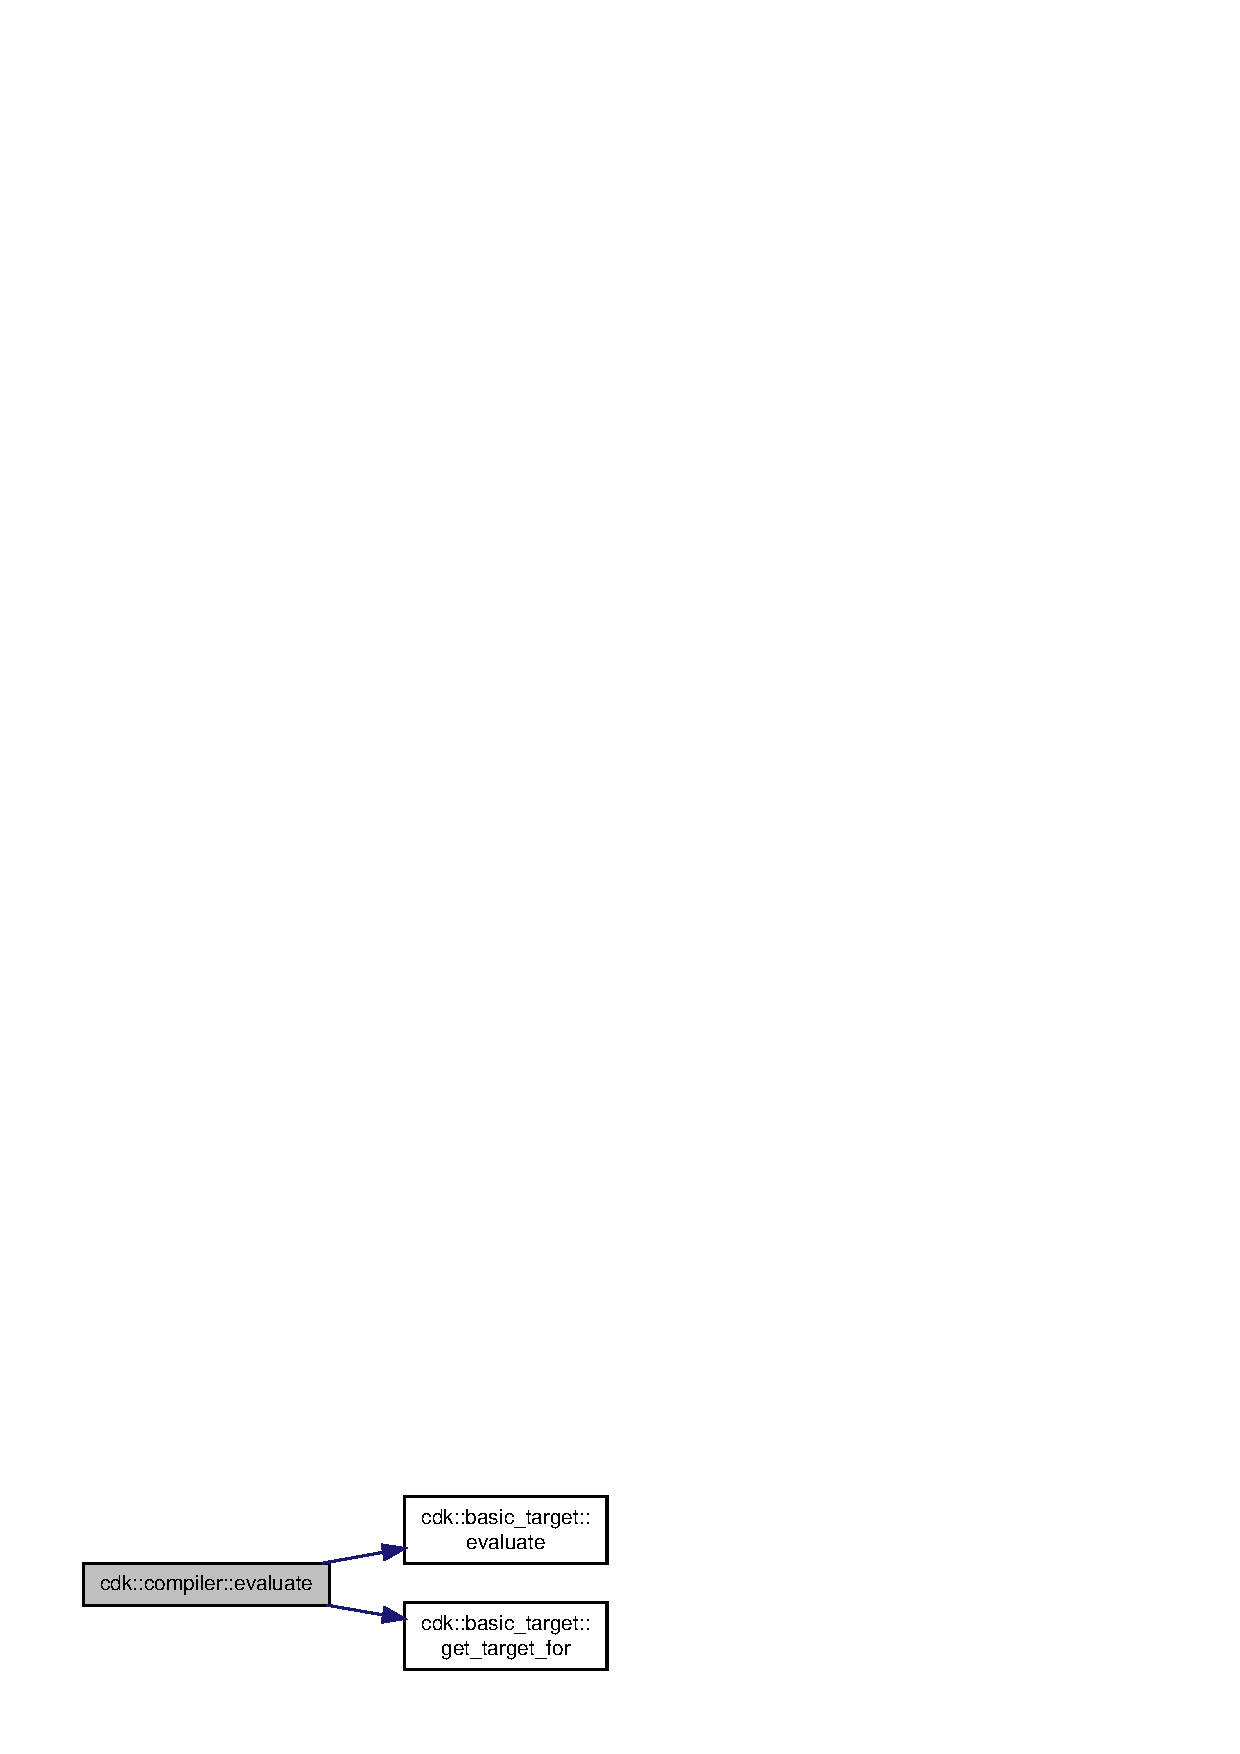
\includegraphics[width=295pt]{classcdk_1_1compiler_a0c0d48f8b1101bb17bd1908785d62eff_cgraph}
\end{center}
\end{figure}


The documentation for this class was generated from the following file\+:\begin{DoxyCompactItemize}
\item 
compiler.\+h\end{DoxyCompactItemize}

\section{cdk\+:\+:data\+\_\+node Class Reference}
\label{classcdk_1_1data__node}\index{cdk\+::data\+\_\+node@{cdk\+::data\+\_\+node}}


{\ttfamily \#include $<$data\+\_\+node.\+h$>$}



Inheritance diagram for cdk\+:\+:data\+\_\+node\+:
\nopagebreak
\begin{figure}[H]
\begin{center}
\leavevmode
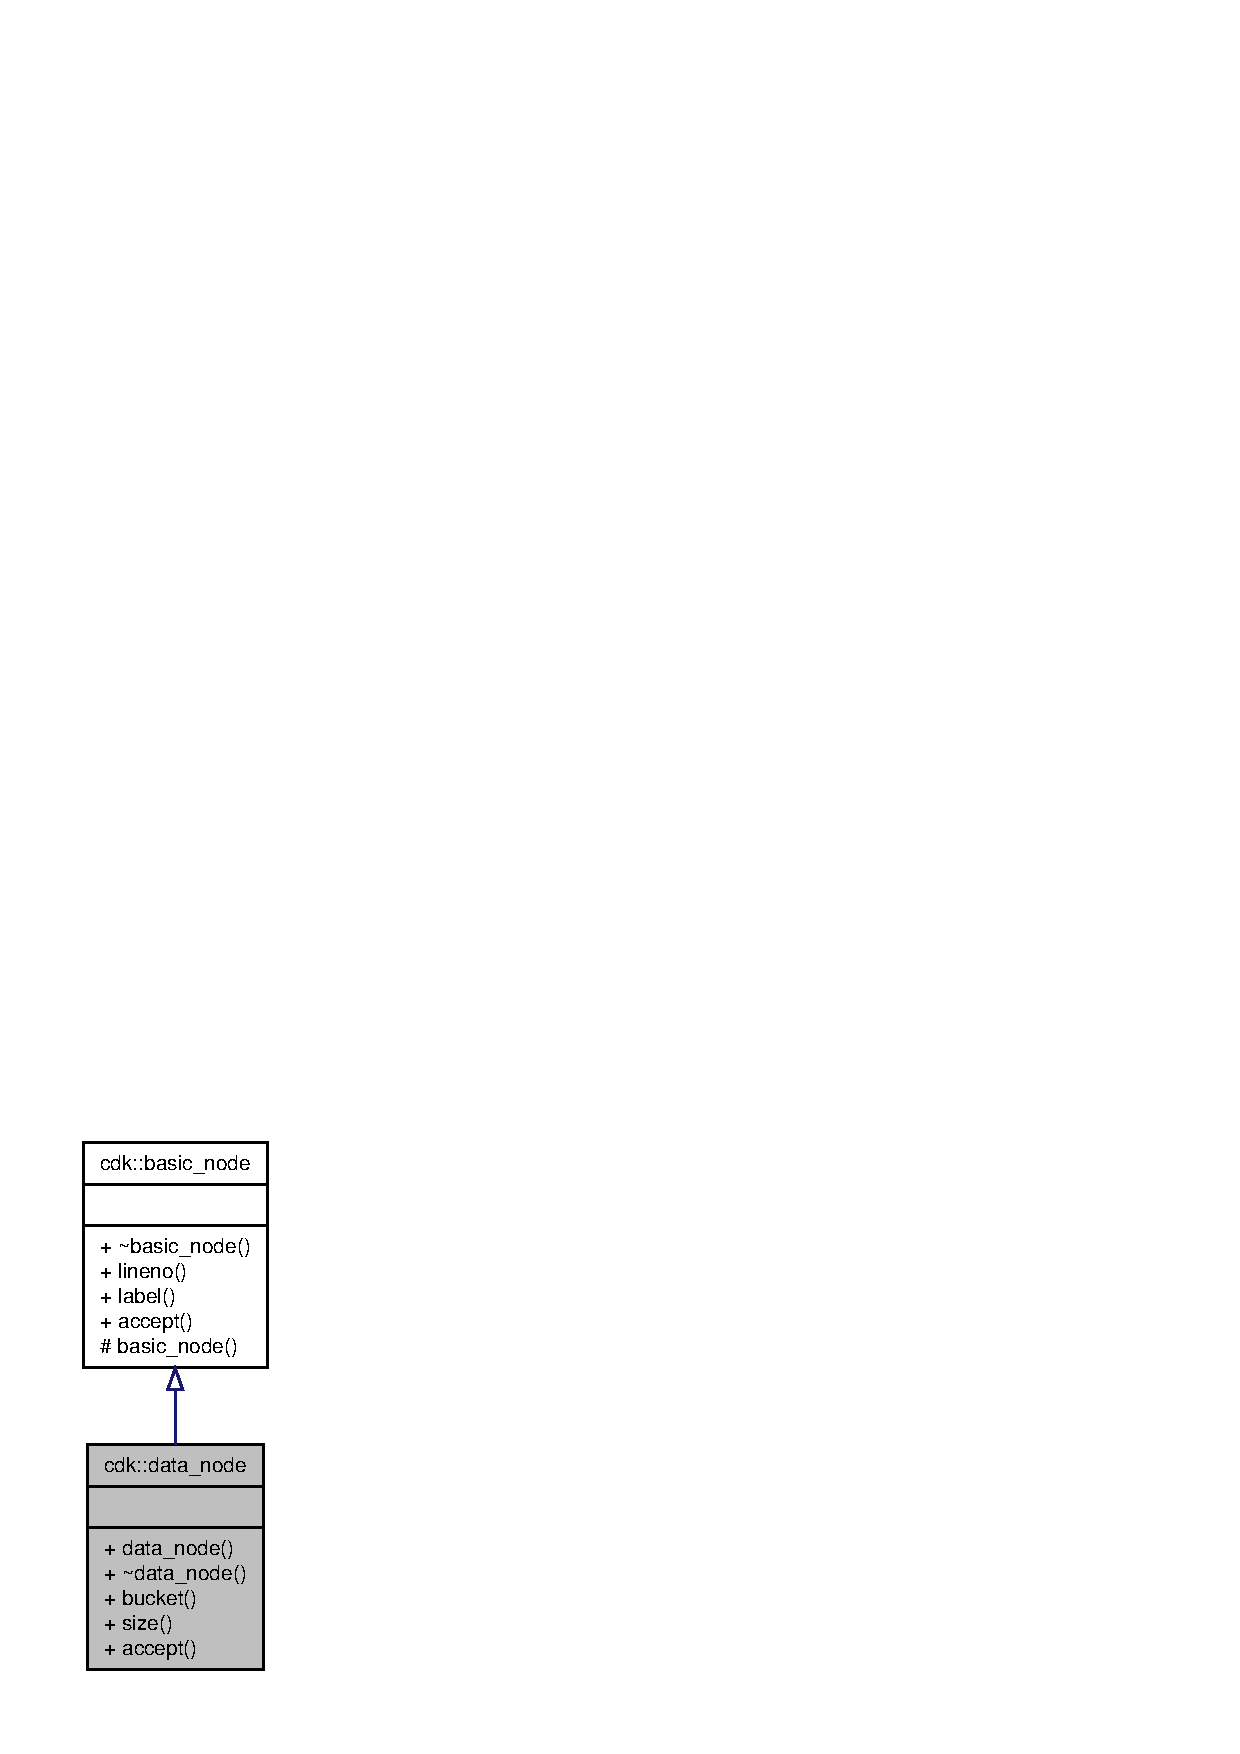
\includegraphics[width=132pt]{classcdk_1_1data__node__inherit__graph}
\end{center}
\end{figure}


Collaboration diagram for cdk\+:\+:data\+\_\+node\+:
\nopagebreak
\begin{figure}[H]
\begin{center}
\leavevmode
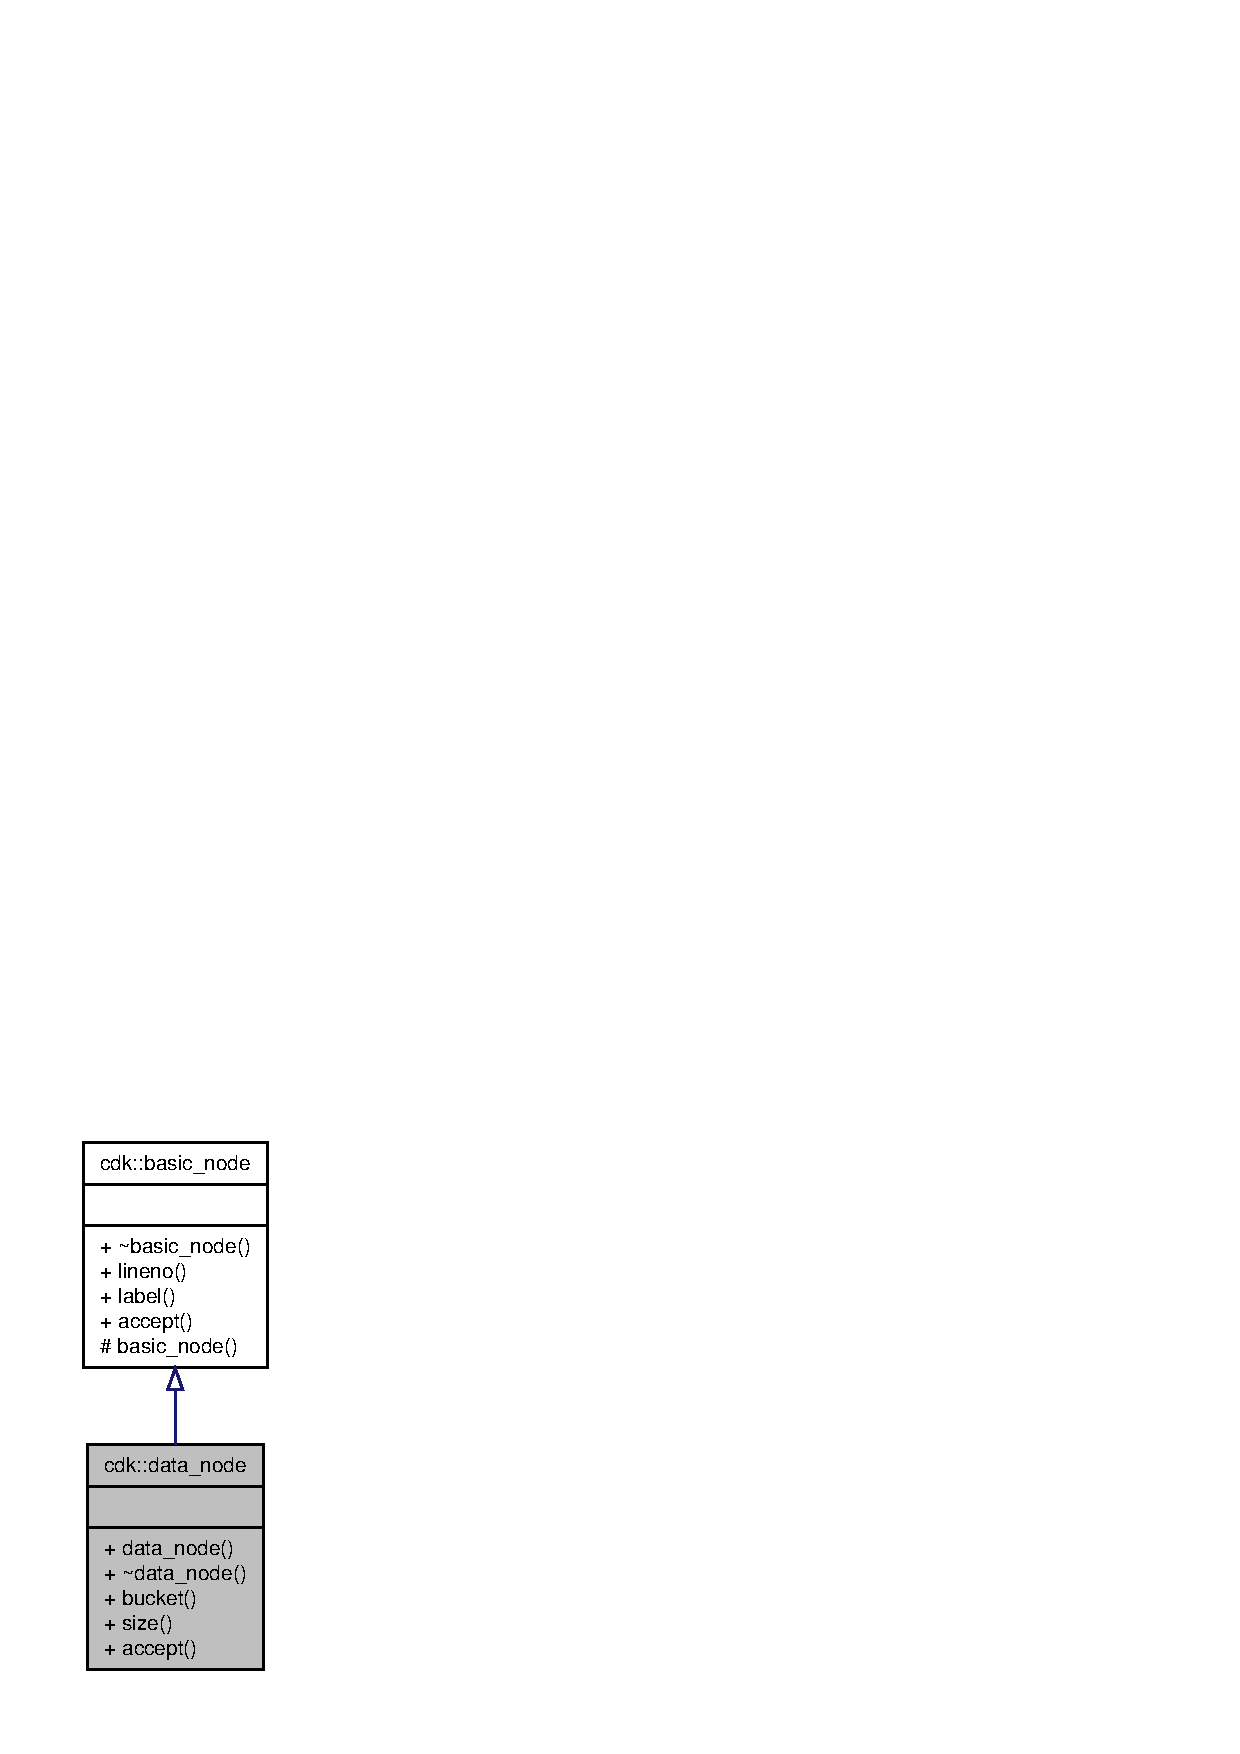
\includegraphics[width=132pt]{classcdk_1_1data__node__coll__graph}
\end{center}
\end{figure}
\subsection*{Public Member Functions}
\begin{DoxyCompactItemize}
\item 
\textbf{ data\+\_\+node} (int \textbf{ lineno}, void $\ast$data, size\+\_\+t nbytes)
\item 
\textbf{ $\sim$data\+\_\+node} ()
\item 
\mbox{\label{classcdk_1_1data__node_a6b68a4bf2fdbce288421128d9c980944}} 
void $\ast$ {\bfseries bucket} ()
\item 
\mbox{\label{classcdk_1_1data__node_a14645461b55cd730f23e95f5ae023bb6}} 
size\+\_\+t {\bfseries size} ()
\item 
void \textbf{ accept} (\textbf{ basic\+\_\+ast\+\_\+visitor} $\ast$sp, int level)
\end{DoxyCompactItemize}
\subsection*{Additional Inherited Members}


\subsection{Detailed Description}
Class for describing syntactic tree leaves for holding data buffers. This class does not inherit from the {\ttfamily Simple} template. 

Definition at line 13 of file data\+\_\+node.\+h.



\subsection{Constructor \& Destructor Documentation}
\mbox{\label{classcdk_1_1data__node_a28f06602d5b68131bed91f668545eb28}} 
\index{cdk\+::data\+\_\+node@{cdk\+::data\+\_\+node}!data\+\_\+node@{data\+\_\+node}}
\index{data\+\_\+node@{data\+\_\+node}!cdk\+::data\+\_\+node@{cdk\+::data\+\_\+node}}
\subsubsection{data\+\_\+node()}
{\footnotesize\ttfamily cdk\+::data\+\_\+node\+::data\+\_\+node (\begin{DoxyParamCaption}\item[{int}]{lineno,  }\item[{void $\ast$}]{data,  }\item[{size\+\_\+t}]{nbytes }\end{DoxyParamCaption})\hspace{0.3cm}{\ttfamily [inline]}}

Constructor for nodes that hold opaque data buffers. Each buffer is characterized by its data and the corresponding data size.


\begin{DoxyParams}{Parameters}
{\em lineno} & the source code line number corresponding to this node \\
\hline
{\em data} & the opaque data buffer \\
\hline
{\em nbytes} & the size (bytes) of the data buffer \\
\hline
\end{DoxyParams}


Definition at line 27 of file data\+\_\+node.\+h.

\mbox{\label{classcdk_1_1data__node_a196cea550b65cde781468694fecc2d9b}} 
\index{cdk\+::data\+\_\+node@{cdk\+::data\+\_\+node}!````~data\+\_\+node@{$\sim$data\+\_\+node}}
\index{````~data\+\_\+node@{$\sim$data\+\_\+node}!cdk\+::data\+\_\+node@{cdk\+::data\+\_\+node}}
\subsubsection{$\sim$data\+\_\+node()}
{\footnotesize\ttfamily cdk\+::data\+\_\+node\+::$\sim$data\+\_\+node (\begin{DoxyParamCaption}{ }\end{DoxyParamCaption})\hspace{0.3cm}{\ttfamily [inline]}}

The destructor. We have defined it explicitly (even though it was not needed) to emphasize that the data buffer is {\bfseries not} destroyed when the node itself dies. 

Definition at line 36 of file data\+\_\+node.\+h.



\subsection{Member Function Documentation}
\mbox{\label{classcdk_1_1data__node_a9d6d6f56201fdfbe965ec399ced60df8}} 
\index{cdk\+::data\+\_\+node@{cdk\+::data\+\_\+node}!accept@{accept}}
\index{accept@{accept}!cdk\+::data\+\_\+node@{cdk\+::data\+\_\+node}}
\subsubsection{accept()}
{\footnotesize\ttfamily void cdk\+::data\+\_\+node\+::accept (\begin{DoxyParamCaption}\item[{\textbf{ basic\+\_\+ast\+\_\+visitor} $\ast$}]{sp,  }\item[{int}]{level }\end{DoxyParamCaption})\hspace{0.3cm}{\ttfamily [inline]}, {\ttfamily [virtual]}}


\begin{DoxyParams}{Parameters}
{\em sp} & semantic processor visitor \\
\hline
{\em level} & syntactic tree level \\
\hline
\end{DoxyParams}


Implements \textbf{ cdk\+::basic\+\_\+node} \doxyref{}{p.}{classcdk_1_1basic__node_ab38adcbc95c46b809961278afae3bf05}.



Definition at line 50 of file data\+\_\+node.\+h.



The documentation for this class was generated from the following file\+:\begin{DoxyCompactItemize}
\item 
ast/data\+\_\+node.\+h\end{DoxyCompactItemize}

\section{cdk\+:\+:div\+\_\+node Class Reference}
\label{classcdk_1_1div__node}\index{cdk\+::div\+\_\+node@{cdk\+::div\+\_\+node}}


{\ttfamily \#include $<$div\+\_\+node.\+h$>$}



Inheritance diagram for cdk\+:\+:div\+\_\+node\+:
\nopagebreak
\begin{figure}[H]
\begin{center}
\leavevmode
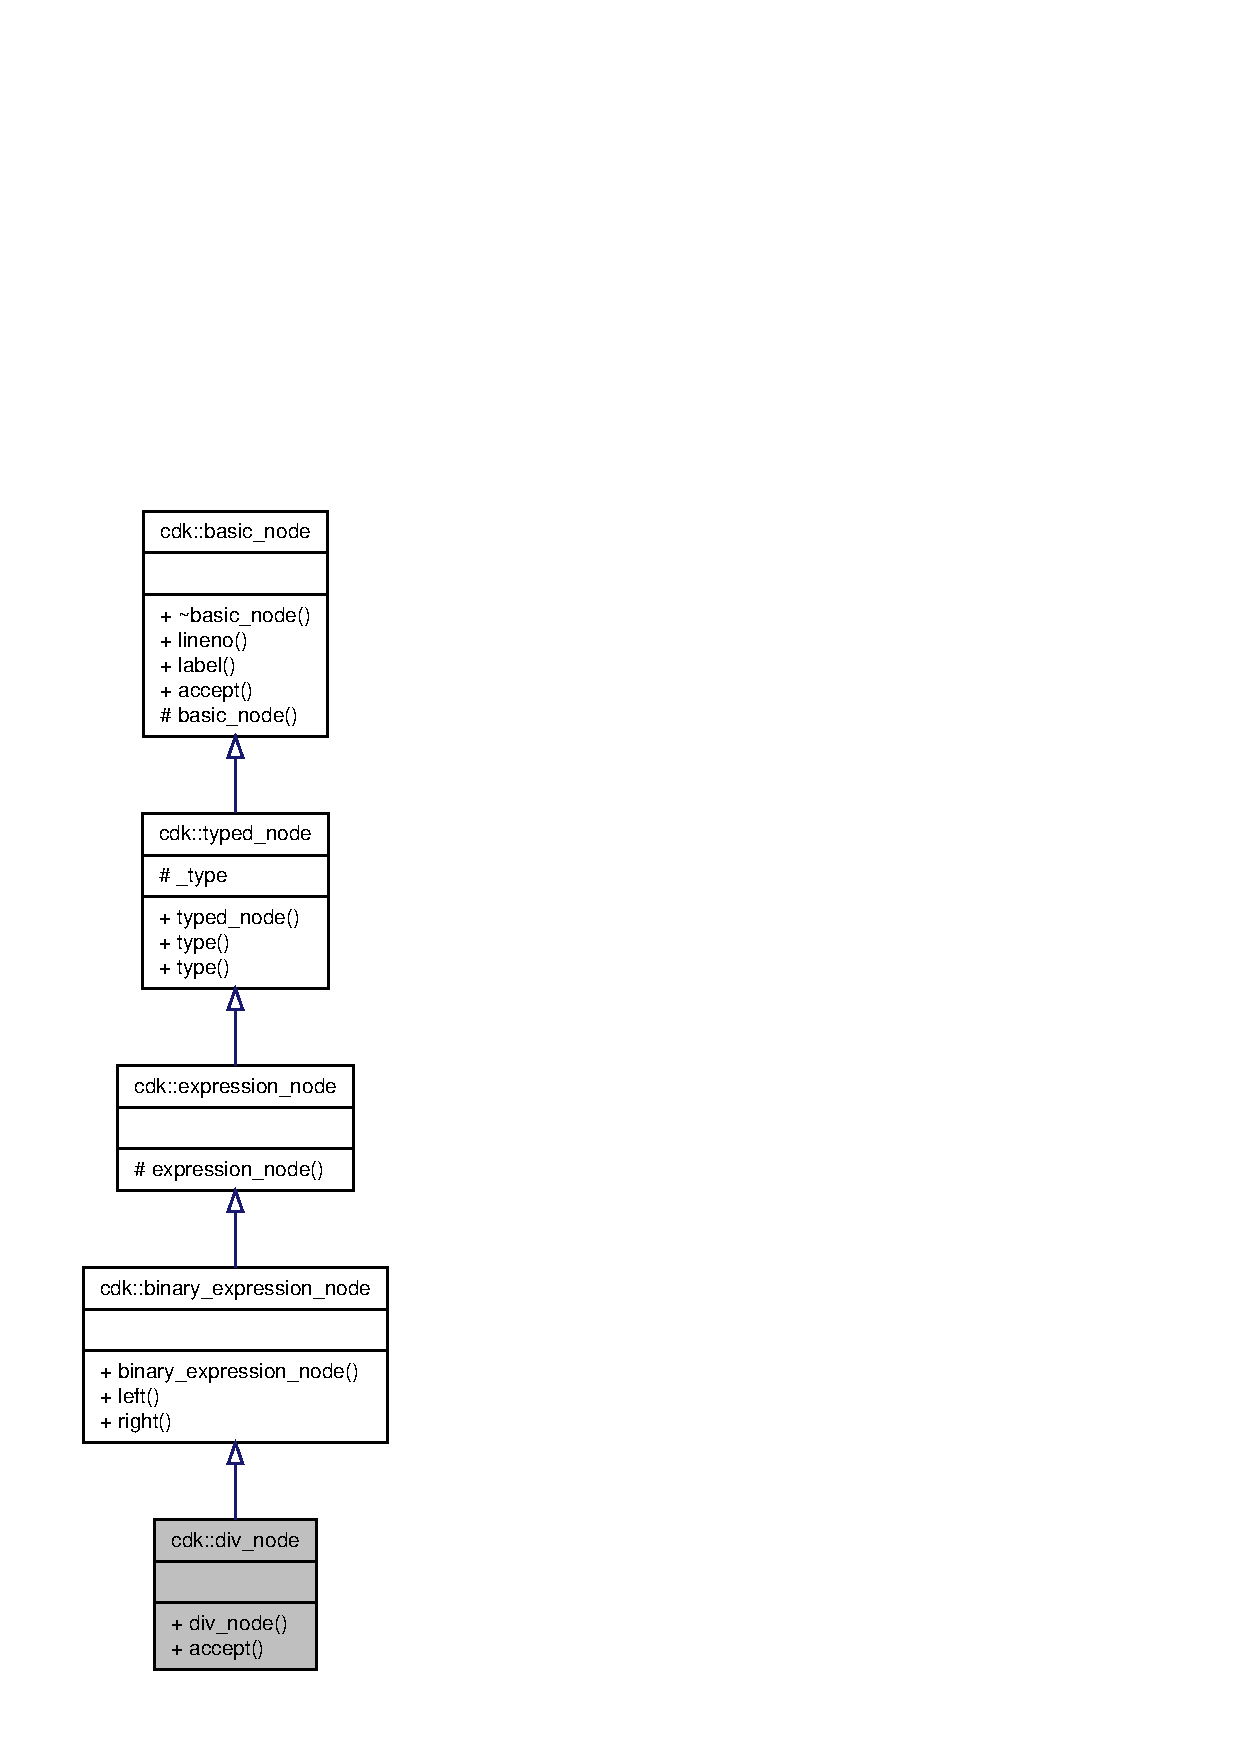
\includegraphics[height=550pt]{classcdk_1_1div__node__inherit__graph}
\end{center}
\end{figure}


Collaboration diagram for cdk\+:\+:div\+\_\+node\+:
\nopagebreak
\begin{figure}[H]
\begin{center}
\leavevmode
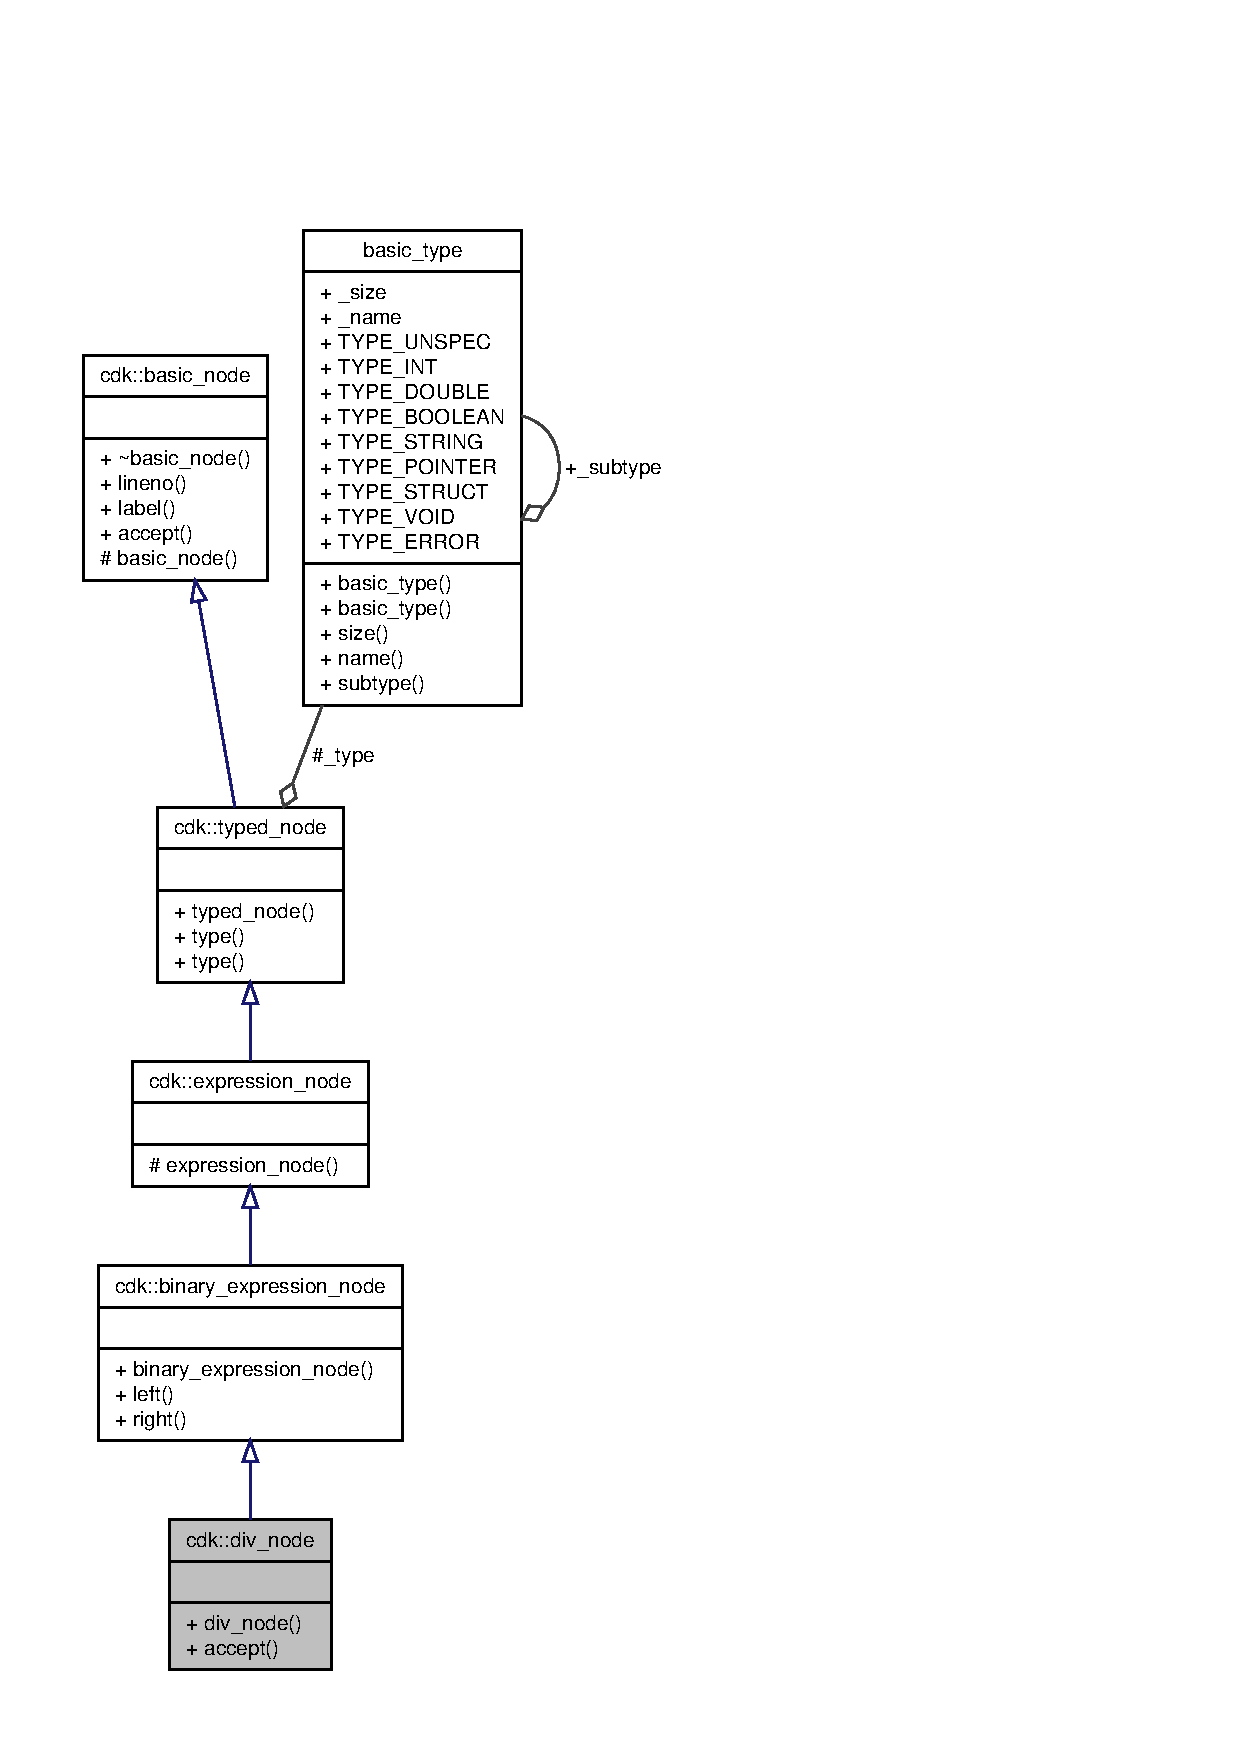
\includegraphics[height=550pt]{classcdk_1_1div__node__coll__graph}
\end{center}
\end{figure}
\subsection*{Public Member Functions}
\begin{DoxyCompactItemize}
\item 
\textbf{ div\+\_\+node} (int \textbf{ lineno}, \textbf{ expression\+\_\+node} $\ast$left, \textbf{ expression\+\_\+node} $\ast$right)
\item 
void \textbf{ accept} (\textbf{ basic\+\_\+ast\+\_\+visitor} $\ast$sp, int level)
\end{DoxyCompactItemize}
\subsection*{Additional Inherited Members}


\subsection{Detailed Description}
Class for describing the division operator 

Definition at line 11 of file div\+\_\+node.\+h.



\subsection{Constructor \& Destructor Documentation}
\mbox{\label{classcdk_1_1div__node_ae5883f44a0fd349b2a8994bc209b155c}} 
\index{cdk\+::div\+\_\+node@{cdk\+::div\+\_\+node}!div\+\_\+node@{div\+\_\+node}}
\index{div\+\_\+node@{div\+\_\+node}!cdk\+::div\+\_\+node@{cdk\+::div\+\_\+node}}
\subsubsection{div\+\_\+node()}
{\footnotesize\ttfamily cdk\+::div\+\_\+node\+::div\+\_\+node (\begin{DoxyParamCaption}\item[{int}]{lineno,  }\item[{\textbf{ expression\+\_\+node} $\ast$}]{left,  }\item[{\textbf{ expression\+\_\+node} $\ast$}]{right }\end{DoxyParamCaption})\hspace{0.3cm}{\ttfamily [inline]}}

\begin{DoxySeeAlso}{See also}
Binary\+Expression 
\end{DoxySeeAlso}


Definition at line 14 of file div\+\_\+node.\+h.



\subsection{Member Function Documentation}
\mbox{\label{classcdk_1_1div__node_a18fdb1b825aeba112a607964f3901a6d}} 
\index{cdk\+::div\+\_\+node@{cdk\+::div\+\_\+node}!accept@{accept}}
\index{accept@{accept}!cdk\+::div\+\_\+node@{cdk\+::div\+\_\+node}}
\subsubsection{accept()}
{\footnotesize\ttfamily void cdk\+::div\+\_\+node\+::accept (\begin{DoxyParamCaption}\item[{\textbf{ basic\+\_\+ast\+\_\+visitor} $\ast$}]{sp,  }\item[{int}]{level }\end{DoxyParamCaption})\hspace{0.3cm}{\ttfamily [inline]}, {\ttfamily [virtual]}}


\begin{DoxyParams}{Parameters}
{\em sp} & semantic processor visitor \\
\hline
{\em level} & syntactic tree level \\
\hline
\end{DoxyParams}


Implements \textbf{ cdk\+::basic\+\_\+node} \doxyref{}{p.}{classcdk_1_1basic__node_ab38adcbc95c46b809961278afae3bf05}.



Definition at line 22 of file div\+\_\+node.\+h.



The documentation for this class was generated from the following file\+:\begin{DoxyCompactItemize}
\item 
ast/div\+\_\+node.\+h\end{DoxyCompactItemize}

\section{cdk\+:\+:double\+\_\+node Class Reference}
\label{classcdk_1_1double__node}\index{cdk\+::double\+\_\+node@{cdk\+::double\+\_\+node}}


{\ttfamily \#include $<$double\+\_\+node.\+h$>$}



Inheritance diagram for cdk\+:\+:double\+\_\+node\+:
\nopagebreak
\begin{figure}[H]
\begin{center}
\leavevmode
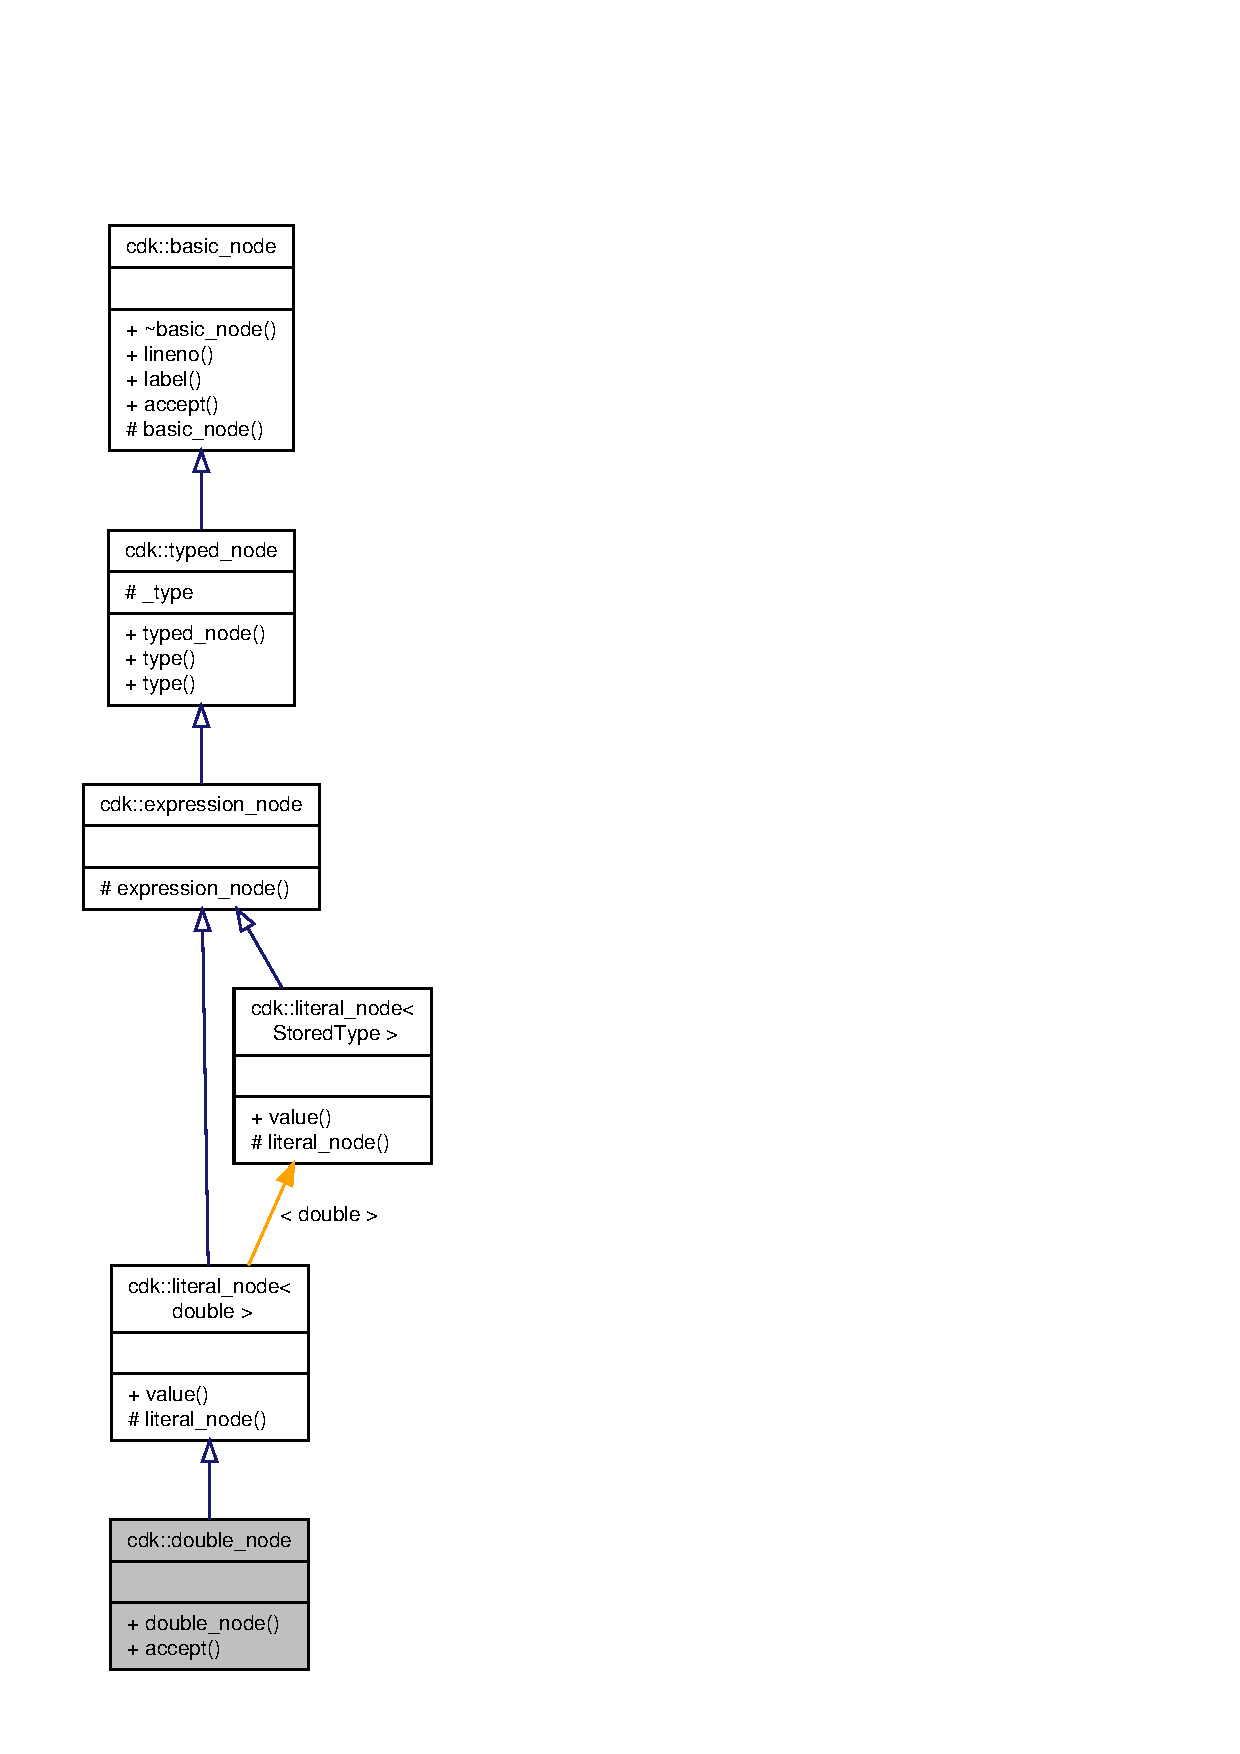
\includegraphics[height=550pt]{classcdk_1_1double__node__inherit__graph}
\end{center}
\end{figure}


Collaboration diagram for cdk\+:\+:double\+\_\+node\+:
\nopagebreak
\begin{figure}[H]
\begin{center}
\leavevmode
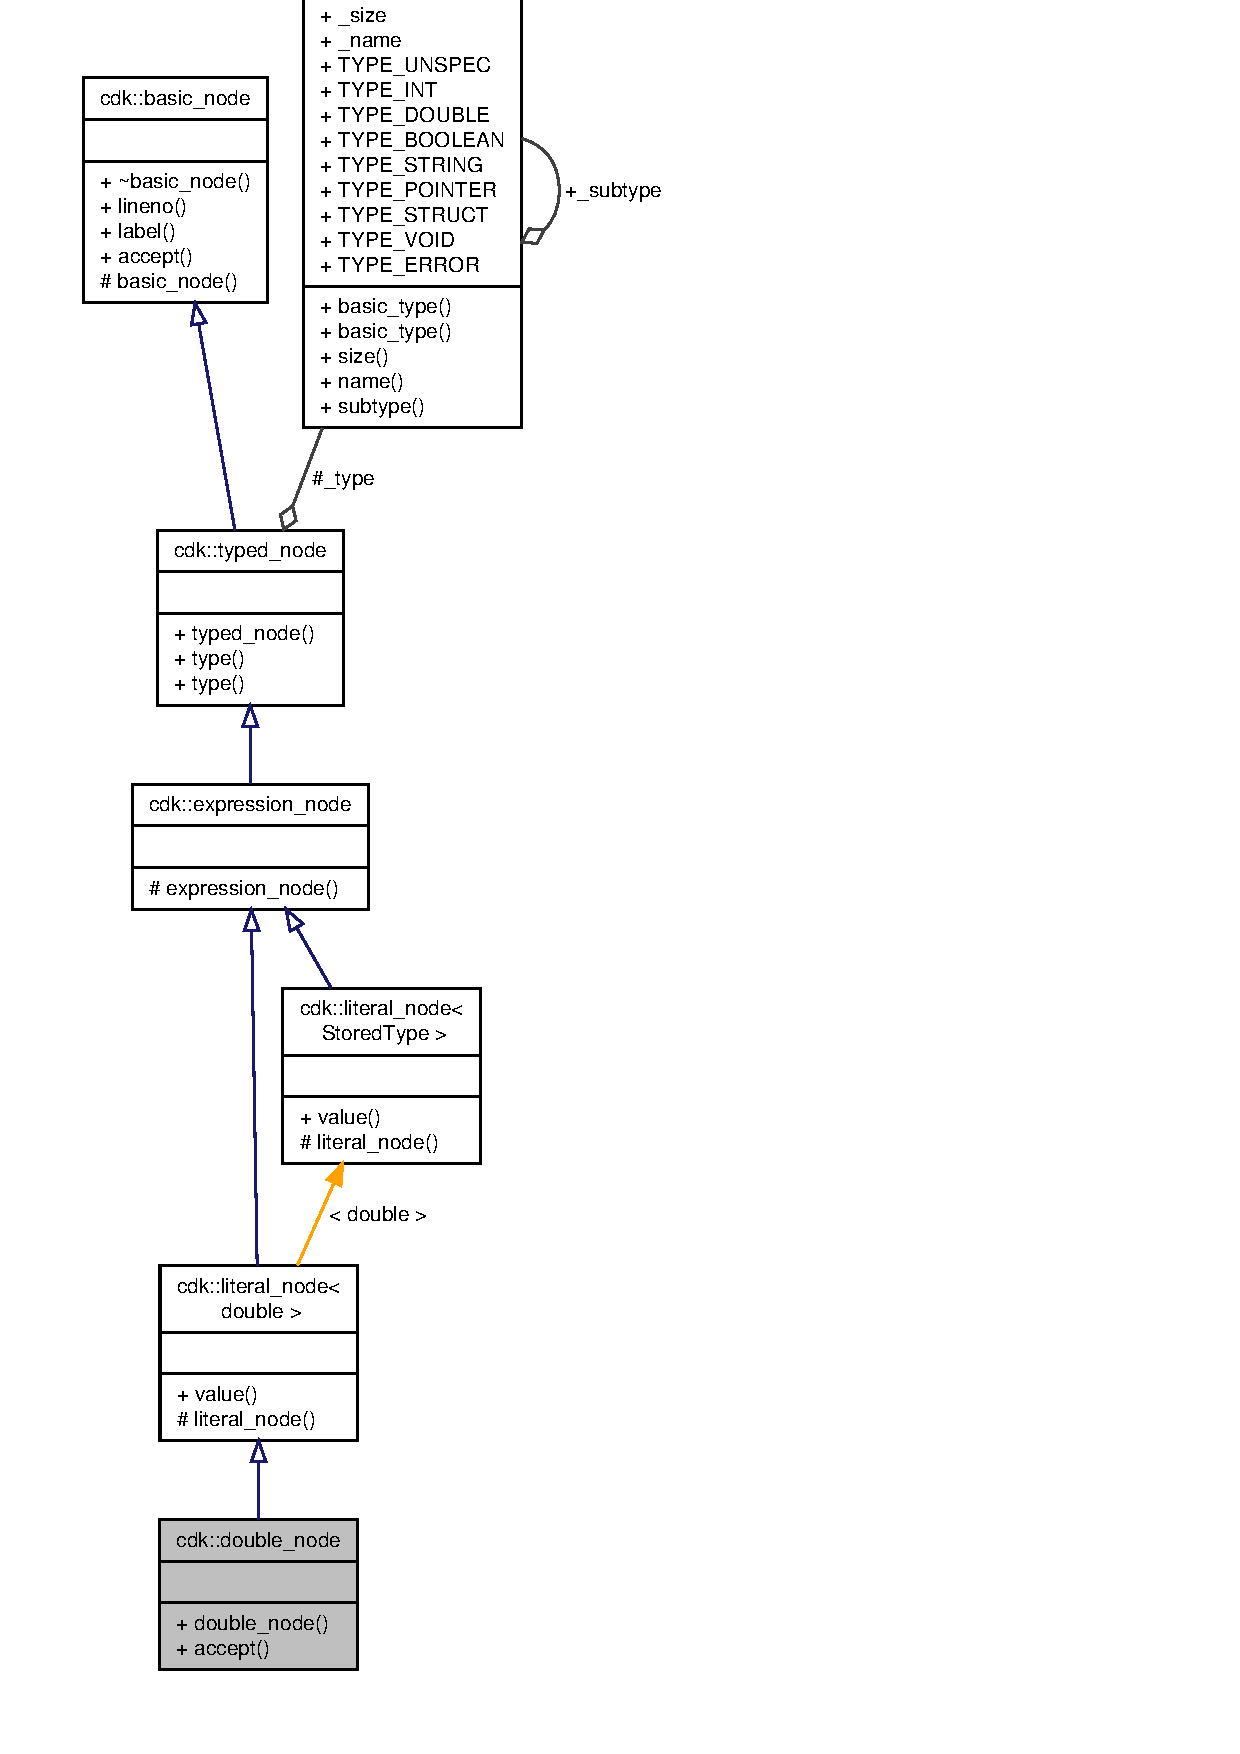
\includegraphics[height=550pt]{classcdk_1_1double__node__coll__graph}
\end{center}
\end{figure}
\subsection*{Public Member Functions}
\begin{DoxyCompactItemize}
\item 
\mbox{\label{classcdk_1_1double__node_aae6671702e1b25b696f7c54fc23a4a99}} 
{\bfseries double\+\_\+node} (int \textbf{ lineno}, double d)
\item 
void \textbf{ accept} (\textbf{ basic\+\_\+ast\+\_\+visitor} $\ast$sp, int level)
\end{DoxyCompactItemize}
\subsection*{Additional Inherited Members}


\subsection{Detailed Description}
Class for describing syntactic tree leaves for holding double precision values. 

Definition at line 12 of file double\+\_\+node.\+h.



\subsection{Member Function Documentation}
\mbox{\label{classcdk_1_1double__node_a3338941e9e94a4f88df4a418092c1ec8}} 
\index{cdk\+::double\+\_\+node@{cdk\+::double\+\_\+node}!accept@{accept}}
\index{accept@{accept}!cdk\+::double\+\_\+node@{cdk\+::double\+\_\+node}}
\subsubsection{accept()}
{\footnotesize\ttfamily void cdk\+::double\+\_\+node\+::accept (\begin{DoxyParamCaption}\item[{\textbf{ basic\+\_\+ast\+\_\+visitor} $\ast$}]{sp,  }\item[{int}]{level }\end{DoxyParamCaption})\hspace{0.3cm}{\ttfamily [inline]}, {\ttfamily [virtual]}}


\begin{DoxyParams}{Parameters}
{\em sp} & semantic processor visitor \\
\hline
{\em level} & syntactic tree level \\
\hline
\end{DoxyParams}


Implements \textbf{ cdk\+::basic\+\_\+node} \doxyref{}{p.}{classcdk_1_1basic__node_ab38adcbc95c46b809961278afae3bf05}.



Definition at line 22 of file double\+\_\+node.\+h.



The documentation for this class was generated from the following file\+:\begin{DoxyCompactItemize}
\item 
ast/double\+\_\+node.\+h\end{DoxyCompactItemize}

\section{cdk\+:\+:eq\+\_\+node Class Reference}
\label{classcdk_1_1eq__node}\index{cdk\+::eq\+\_\+node@{cdk\+::eq\+\_\+node}}


{\ttfamily \#include $<$eq\+\_\+node.\+h$>$}



Inheritance diagram for cdk\+:\+:eq\+\_\+node\+:
\nopagebreak
\begin{figure}[H]
\begin{center}
\leavevmode
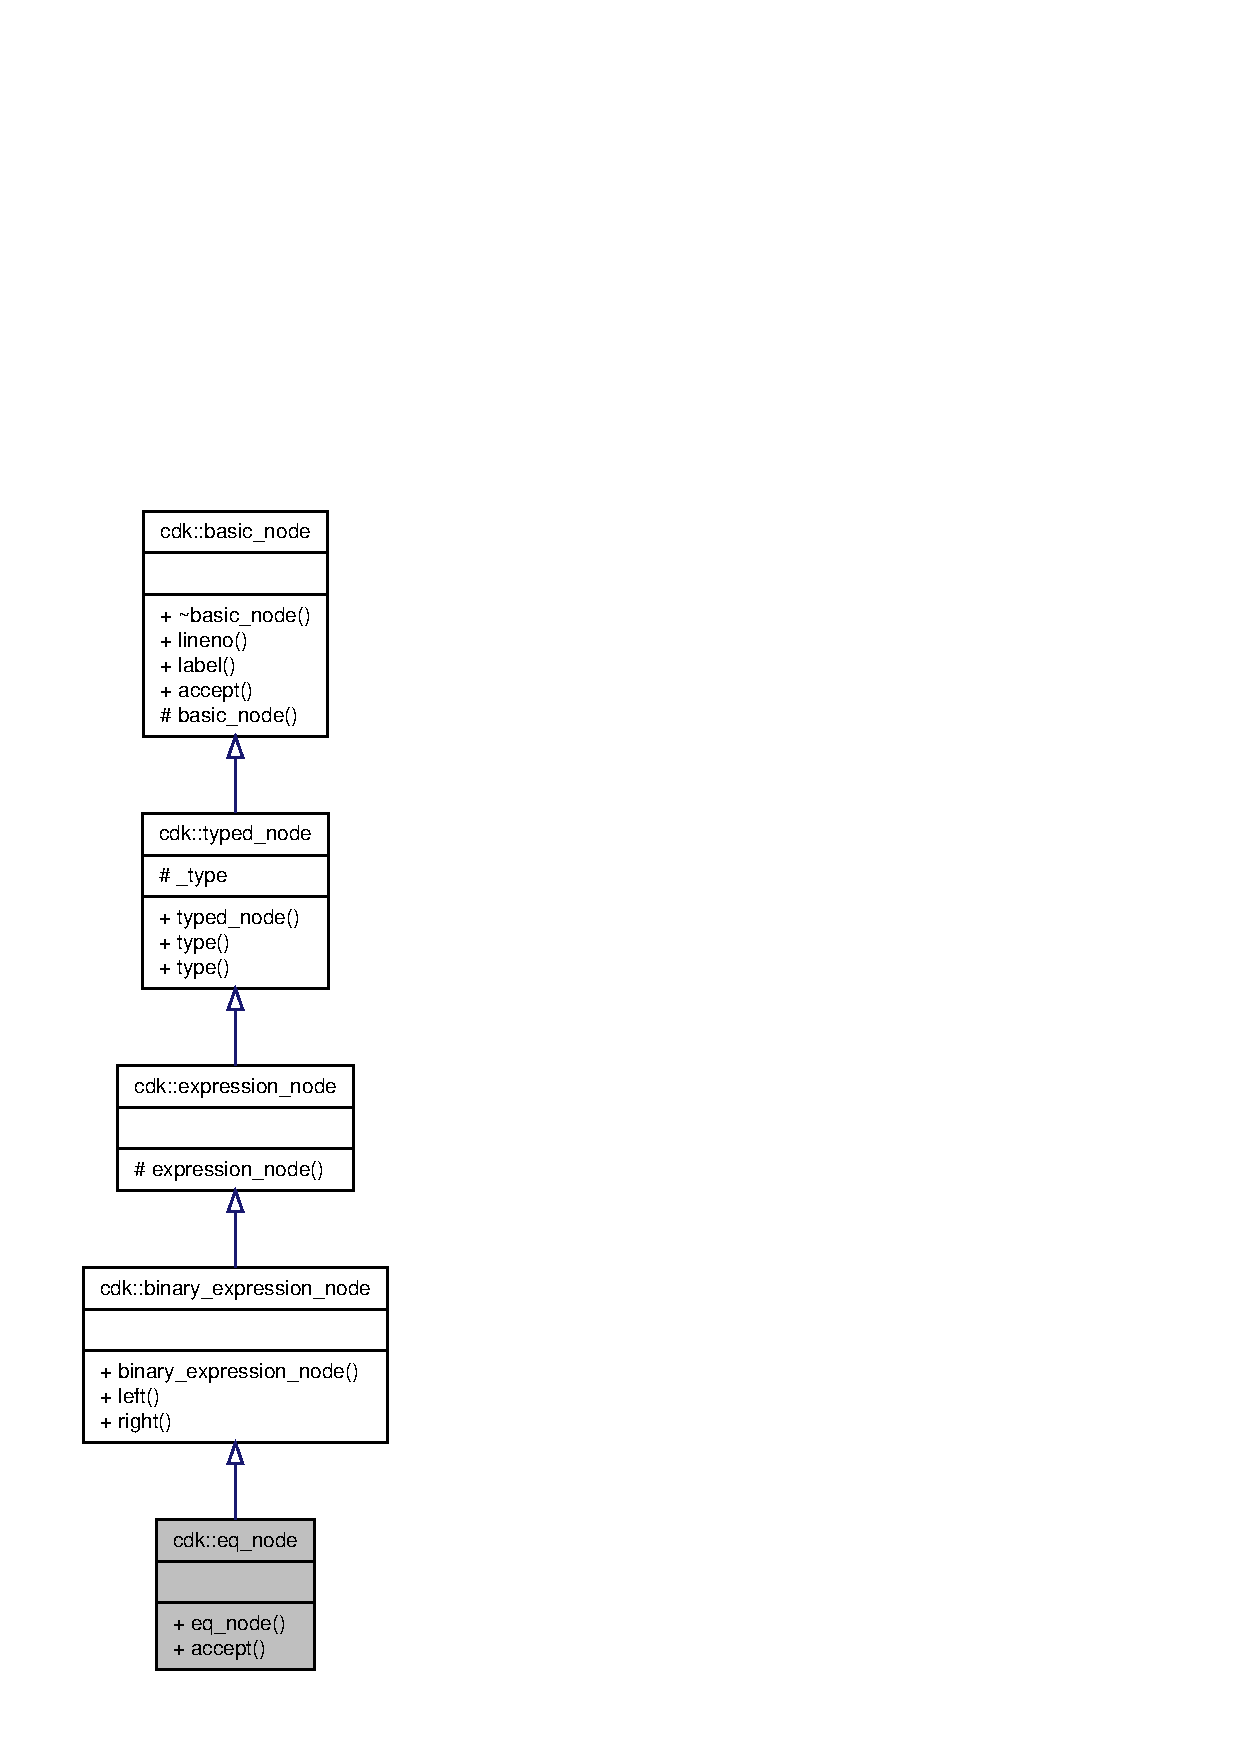
\includegraphics[height=550pt]{classcdk_1_1eq__node__inherit__graph}
\end{center}
\end{figure}


Collaboration diagram for cdk\+:\+:eq\+\_\+node\+:
\nopagebreak
\begin{figure}[H]
\begin{center}
\leavevmode
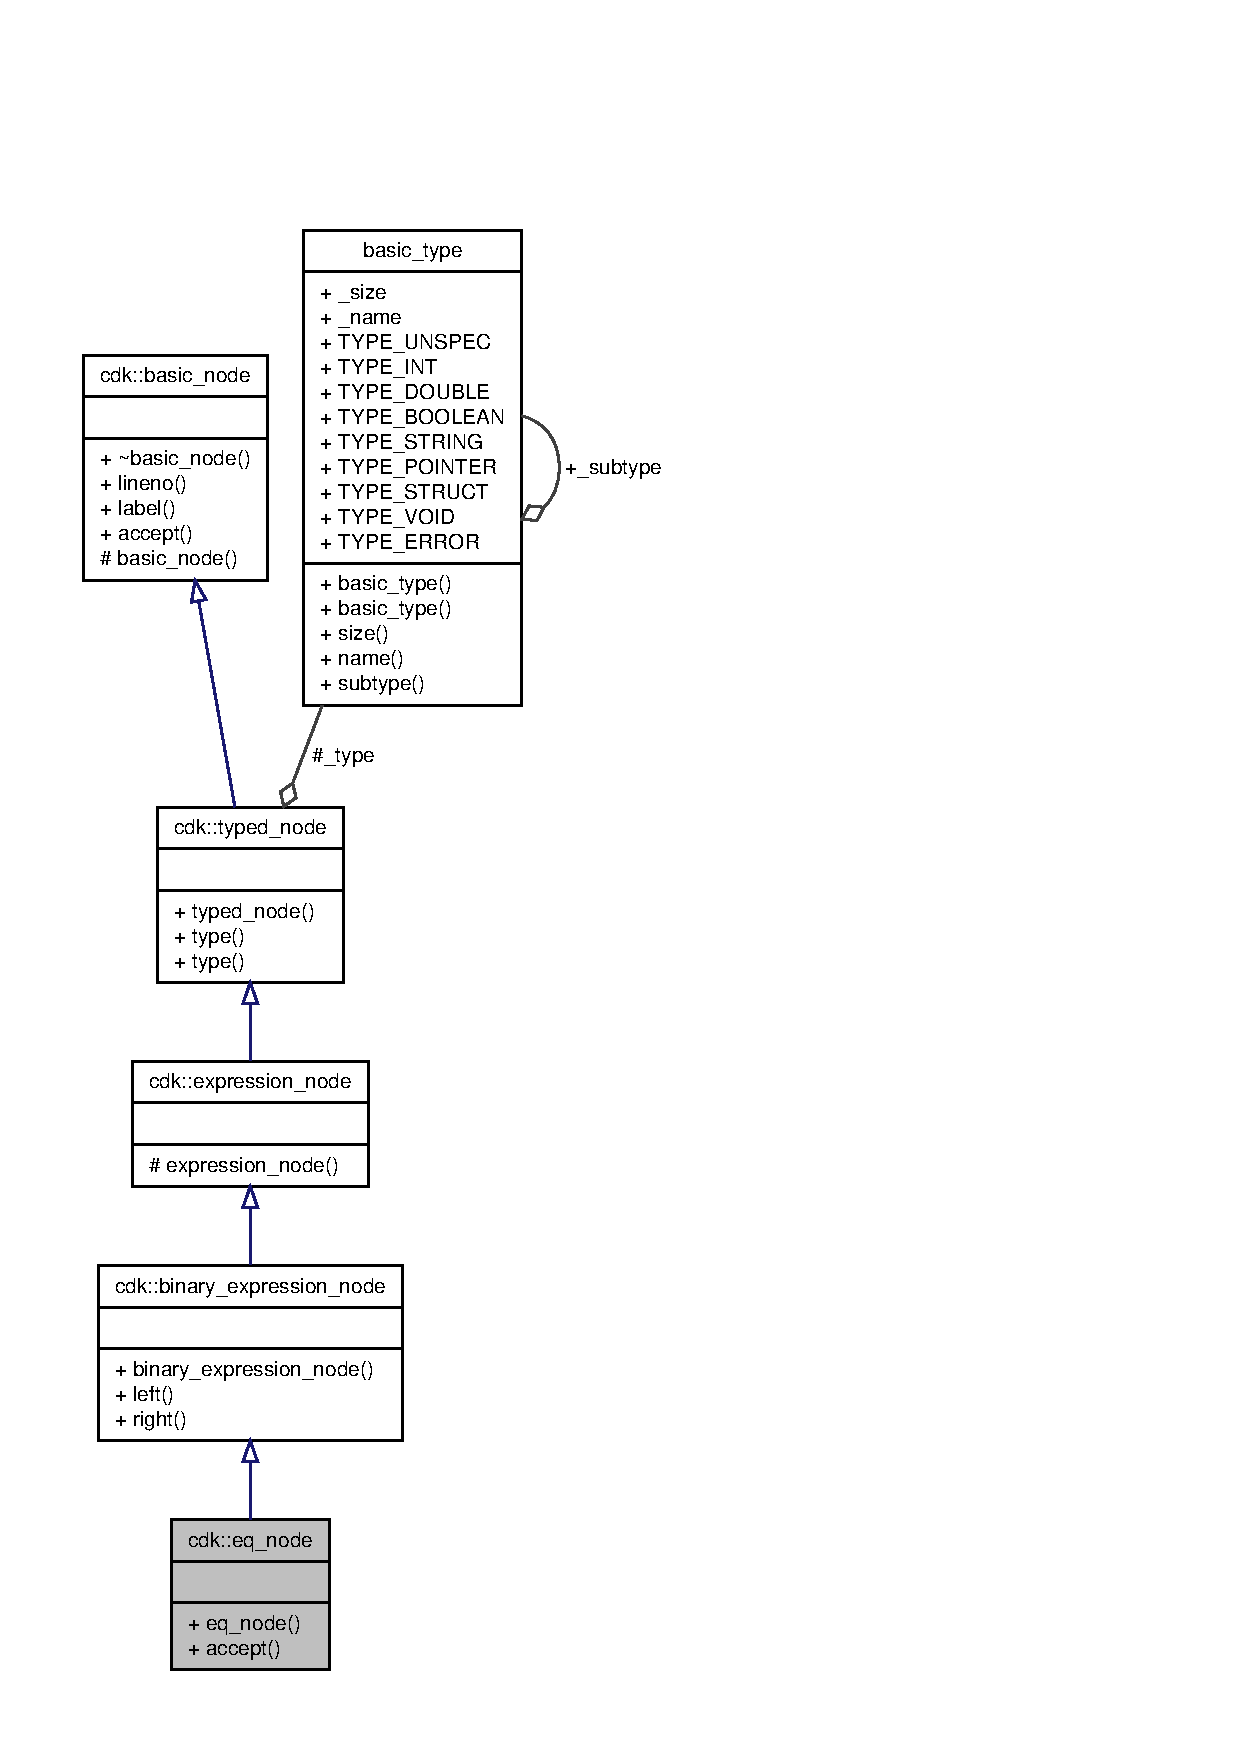
\includegraphics[height=550pt]{classcdk_1_1eq__node__coll__graph}
\end{center}
\end{figure}
\subsection*{Public Member Functions}
\begin{DoxyCompactItemize}
\item 
\textbf{ eq\+\_\+node} (int \textbf{ lineno}, \textbf{ expression\+\_\+node} $\ast$left, \textbf{ expression\+\_\+node} $\ast$right)
\item 
void \textbf{ accept} (\textbf{ basic\+\_\+ast\+\_\+visitor} $\ast$sp, int level)
\end{DoxyCompactItemize}
\subsection*{Additional Inherited Members}


\subsection{Detailed Description}
Class for describing the equality operator 

Definition at line 11 of file eq\+\_\+node.\+h.



\subsection{Constructor \& Destructor Documentation}
\mbox{\label{classcdk_1_1eq__node_a69cb18aa9ce0d7907192204fe24f4518}} 
\index{cdk\+::eq\+\_\+node@{cdk\+::eq\+\_\+node}!eq\+\_\+node@{eq\+\_\+node}}
\index{eq\+\_\+node@{eq\+\_\+node}!cdk\+::eq\+\_\+node@{cdk\+::eq\+\_\+node}}
\subsubsection{eq\+\_\+node()}
{\footnotesize\ttfamily cdk\+::eq\+\_\+node\+::eq\+\_\+node (\begin{DoxyParamCaption}\item[{int}]{lineno,  }\item[{\textbf{ expression\+\_\+node} $\ast$}]{left,  }\item[{\textbf{ expression\+\_\+node} $\ast$}]{right }\end{DoxyParamCaption})\hspace{0.3cm}{\ttfamily [inline]}}


\begin{DoxyParams}{Parameters}
{\em lineno} & source code line number for this node \\
\hline
{\em left} & first operand \\
\hline
{\em right} & second operand \\
\hline
\end{DoxyParams}


Definition at line 19 of file eq\+\_\+node.\+h.



\subsection{Member Function Documentation}
\mbox{\label{classcdk_1_1eq__node_ac874f2c13fc2f66ce23b08d99594368e}} 
\index{cdk\+::eq\+\_\+node@{cdk\+::eq\+\_\+node}!accept@{accept}}
\index{accept@{accept}!cdk\+::eq\+\_\+node@{cdk\+::eq\+\_\+node}}
\subsubsection{accept()}
{\footnotesize\ttfamily void cdk\+::eq\+\_\+node\+::accept (\begin{DoxyParamCaption}\item[{\textbf{ basic\+\_\+ast\+\_\+visitor} $\ast$}]{sp,  }\item[{int}]{level }\end{DoxyParamCaption})\hspace{0.3cm}{\ttfamily [inline]}, {\ttfamily [virtual]}}


\begin{DoxyParams}{Parameters}
{\em sp} & semantic processor visitor \\
\hline
{\em level} & syntactic tree level \\
\hline
\end{DoxyParams}


Implements \textbf{ cdk\+::basic\+\_\+node} \doxyref{}{p.}{classcdk_1_1basic__node_ab38adcbc95c46b809961278afae3bf05}.



Definition at line 27 of file eq\+\_\+node.\+h.



The documentation for this class was generated from the following file\+:\begin{DoxyCompactItemize}
\item 
ast/eq\+\_\+node.\+h\end{DoxyCompactItemize}

\section{cdk\+:\+:expression\+\_\+node Class Reference}
\label{classcdk_1_1expression__node}\index{cdk\+::expression\+\_\+node@{cdk\+::expression\+\_\+node}}


{\ttfamily \#include $<$expression\+\_\+node.\+h$>$}



Inheritance diagram for cdk\+:\+:expression\+\_\+node\+:
\nopagebreak
\begin{figure}[H]
\begin{center}
\leavevmode
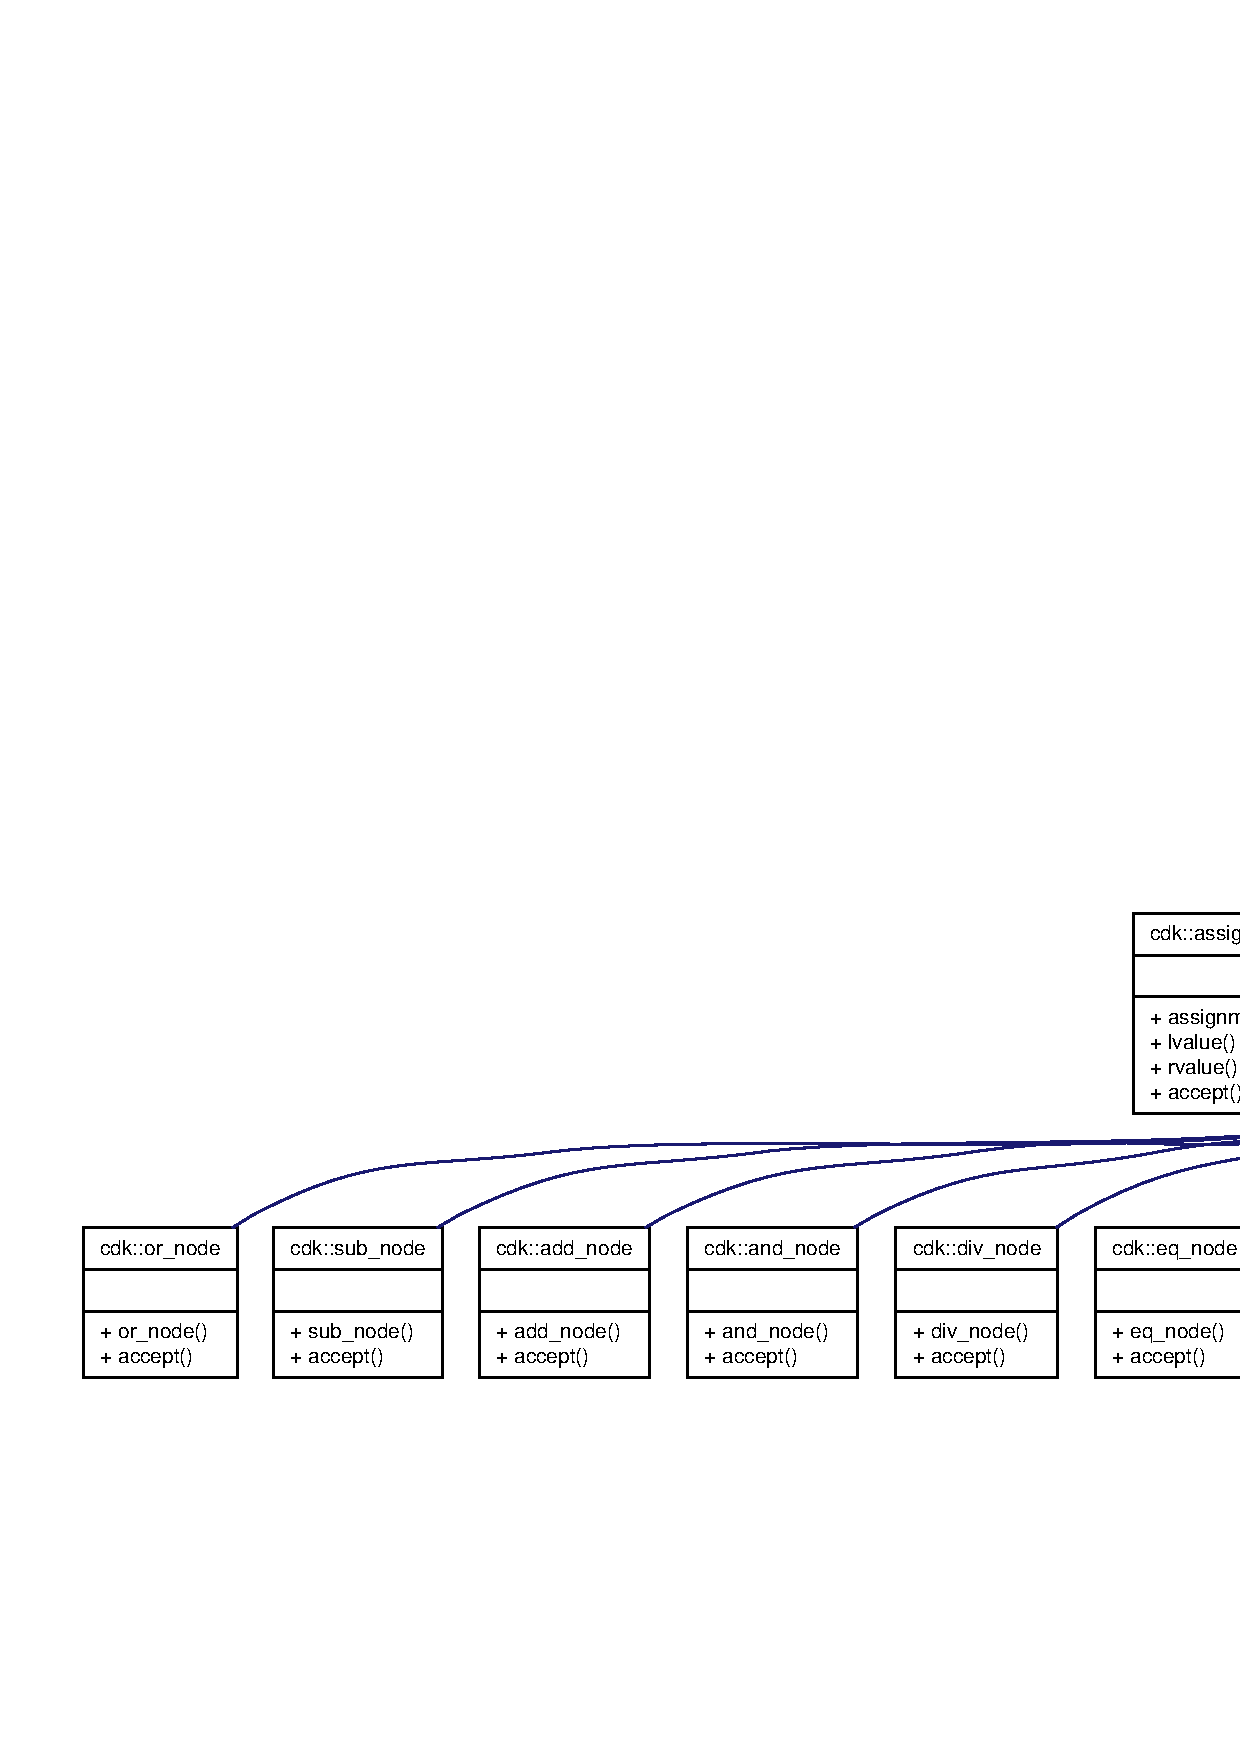
\includegraphics[width=350pt]{classcdk_1_1expression__node__inherit__graph}
\end{center}
\end{figure}


Collaboration diagram for cdk\+:\+:expression\+\_\+node\+:
\nopagebreak
\begin{figure}[H]
\begin{center}
\leavevmode
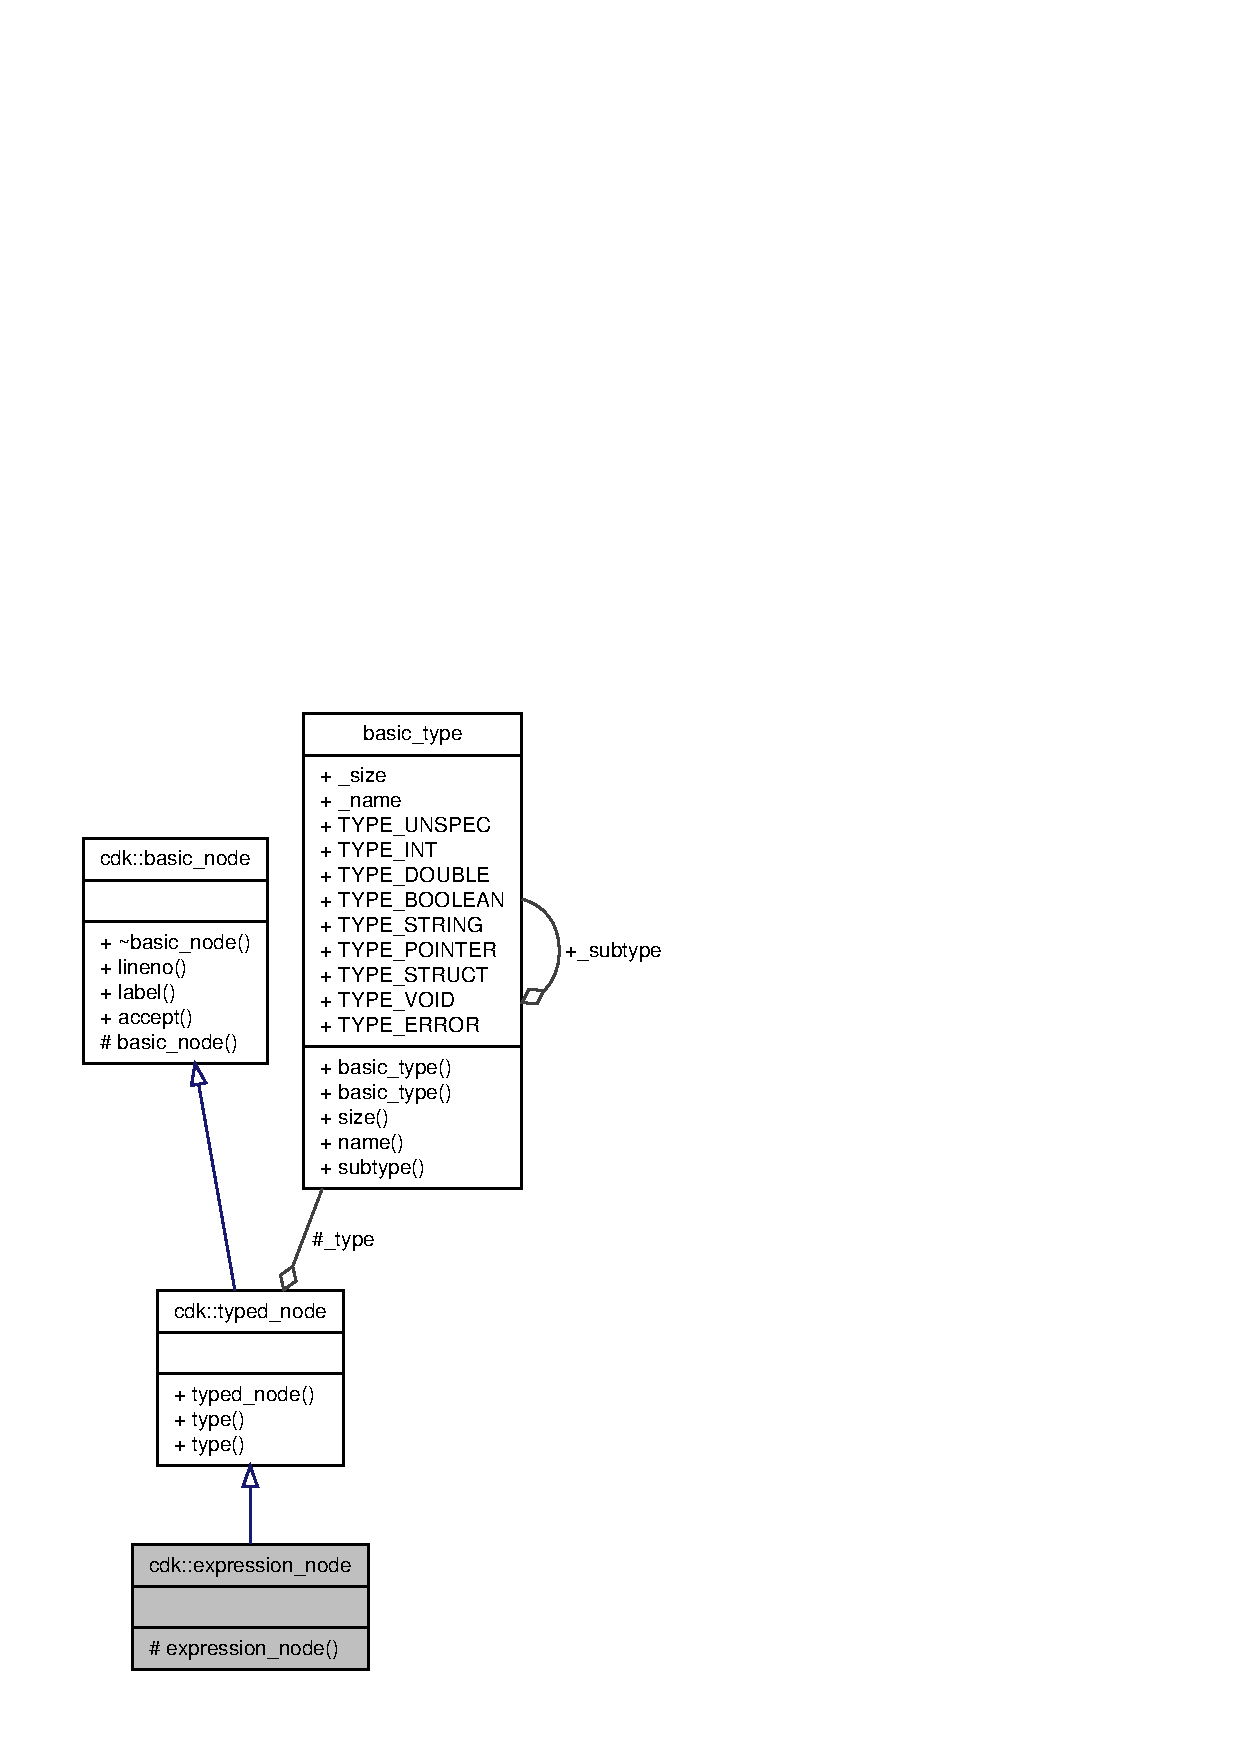
\includegraphics[width=322pt]{classcdk_1_1expression__node__coll__graph}
\end{center}
\end{figure}
\subsection*{Protected Member Functions}
\begin{DoxyCompactItemize}
\item 
\textbf{ expression\+\_\+node} (int \textbf{ lineno})
\end{DoxyCompactItemize}
\subsection*{Additional Inherited Members}


\subsection{Detailed Description}
Expressions are typed nodes that have a value. 

Definition at line 11 of file expression\+\_\+node.\+h.



\subsection{Constructor \& Destructor Documentation}
\mbox{\label{classcdk_1_1expression__node_a026555785146a09f2d53d56e1bb1e984}} 
\index{cdk\+::expression\+\_\+node@{cdk\+::expression\+\_\+node}!expression\+\_\+node@{expression\+\_\+node}}
\index{expression\+\_\+node@{expression\+\_\+node}!cdk\+::expression\+\_\+node@{cdk\+::expression\+\_\+node}}
\subsubsection{expression\+\_\+node()}
{\footnotesize\ttfamily cdk\+::expression\+\_\+node\+::expression\+\_\+node (\begin{DoxyParamCaption}\item[{int}]{lineno }\end{DoxyParamCaption})\hspace{0.3cm}{\ttfamily [inline]}, {\ttfamily [protected]}}


\begin{DoxyParams}{Parameters}
{\em lineno} & the source code line corresponding to the node \\
\hline
\end{DoxyParams}


Definition at line 17 of file expression\+\_\+node.\+h.



The documentation for this class was generated from the following file\+:\begin{DoxyCompactItemize}
\item 
ast/expression\+\_\+node.\+h\end{DoxyCompactItemize}

\section{cdk\+:\+:ge\+\_\+node Class Reference}
\label{classcdk_1_1ge__node}\index{cdk\+::ge\+\_\+node@{cdk\+::ge\+\_\+node}}


{\ttfamily \#include $<$ge\+\_\+node.\+h$>$}



Inheritance diagram for cdk\+:\+:ge\+\_\+node\+:
\nopagebreak
\begin{figure}[H]
\begin{center}
\leavevmode
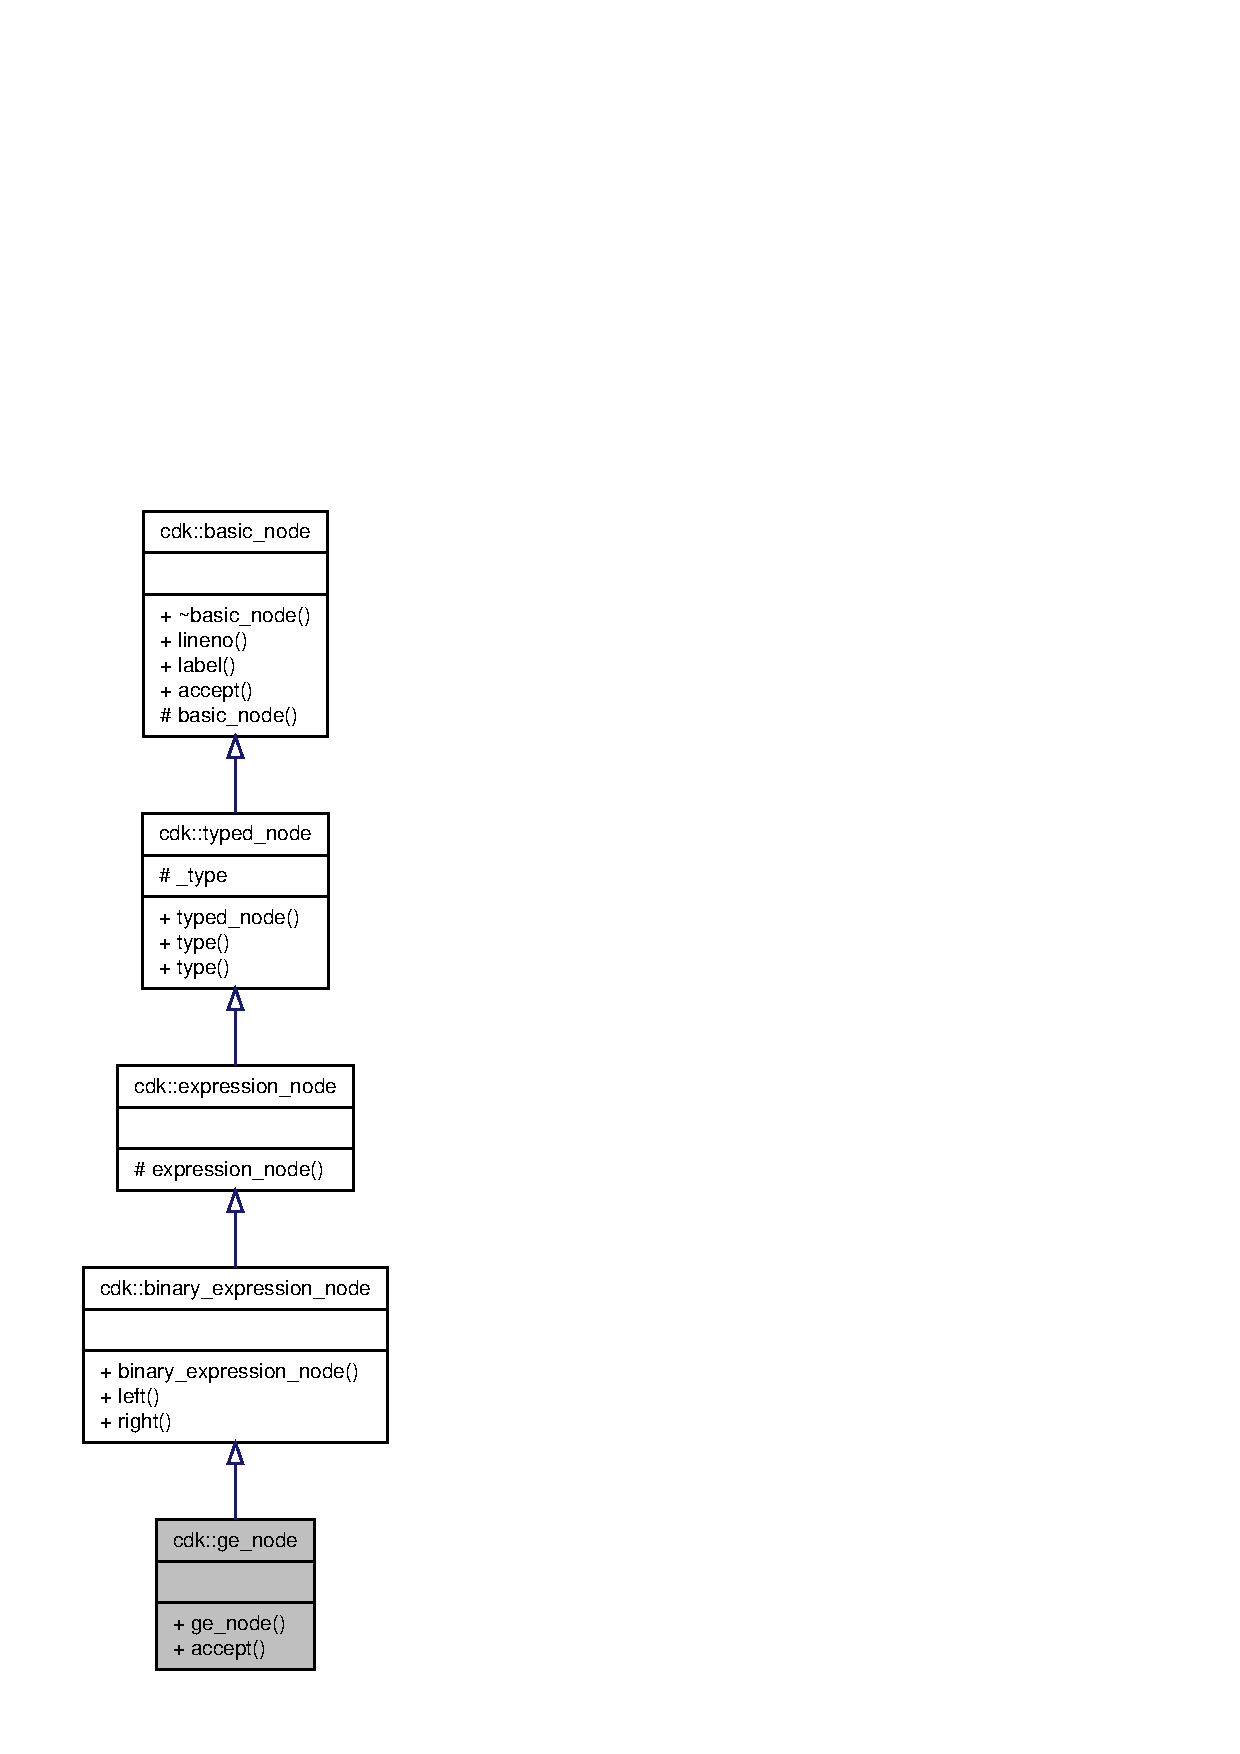
\includegraphics[height=550pt]{classcdk_1_1ge__node__inherit__graph}
\end{center}
\end{figure}


Collaboration diagram for cdk\+:\+:ge\+\_\+node\+:
\nopagebreak
\begin{figure}[H]
\begin{center}
\leavevmode
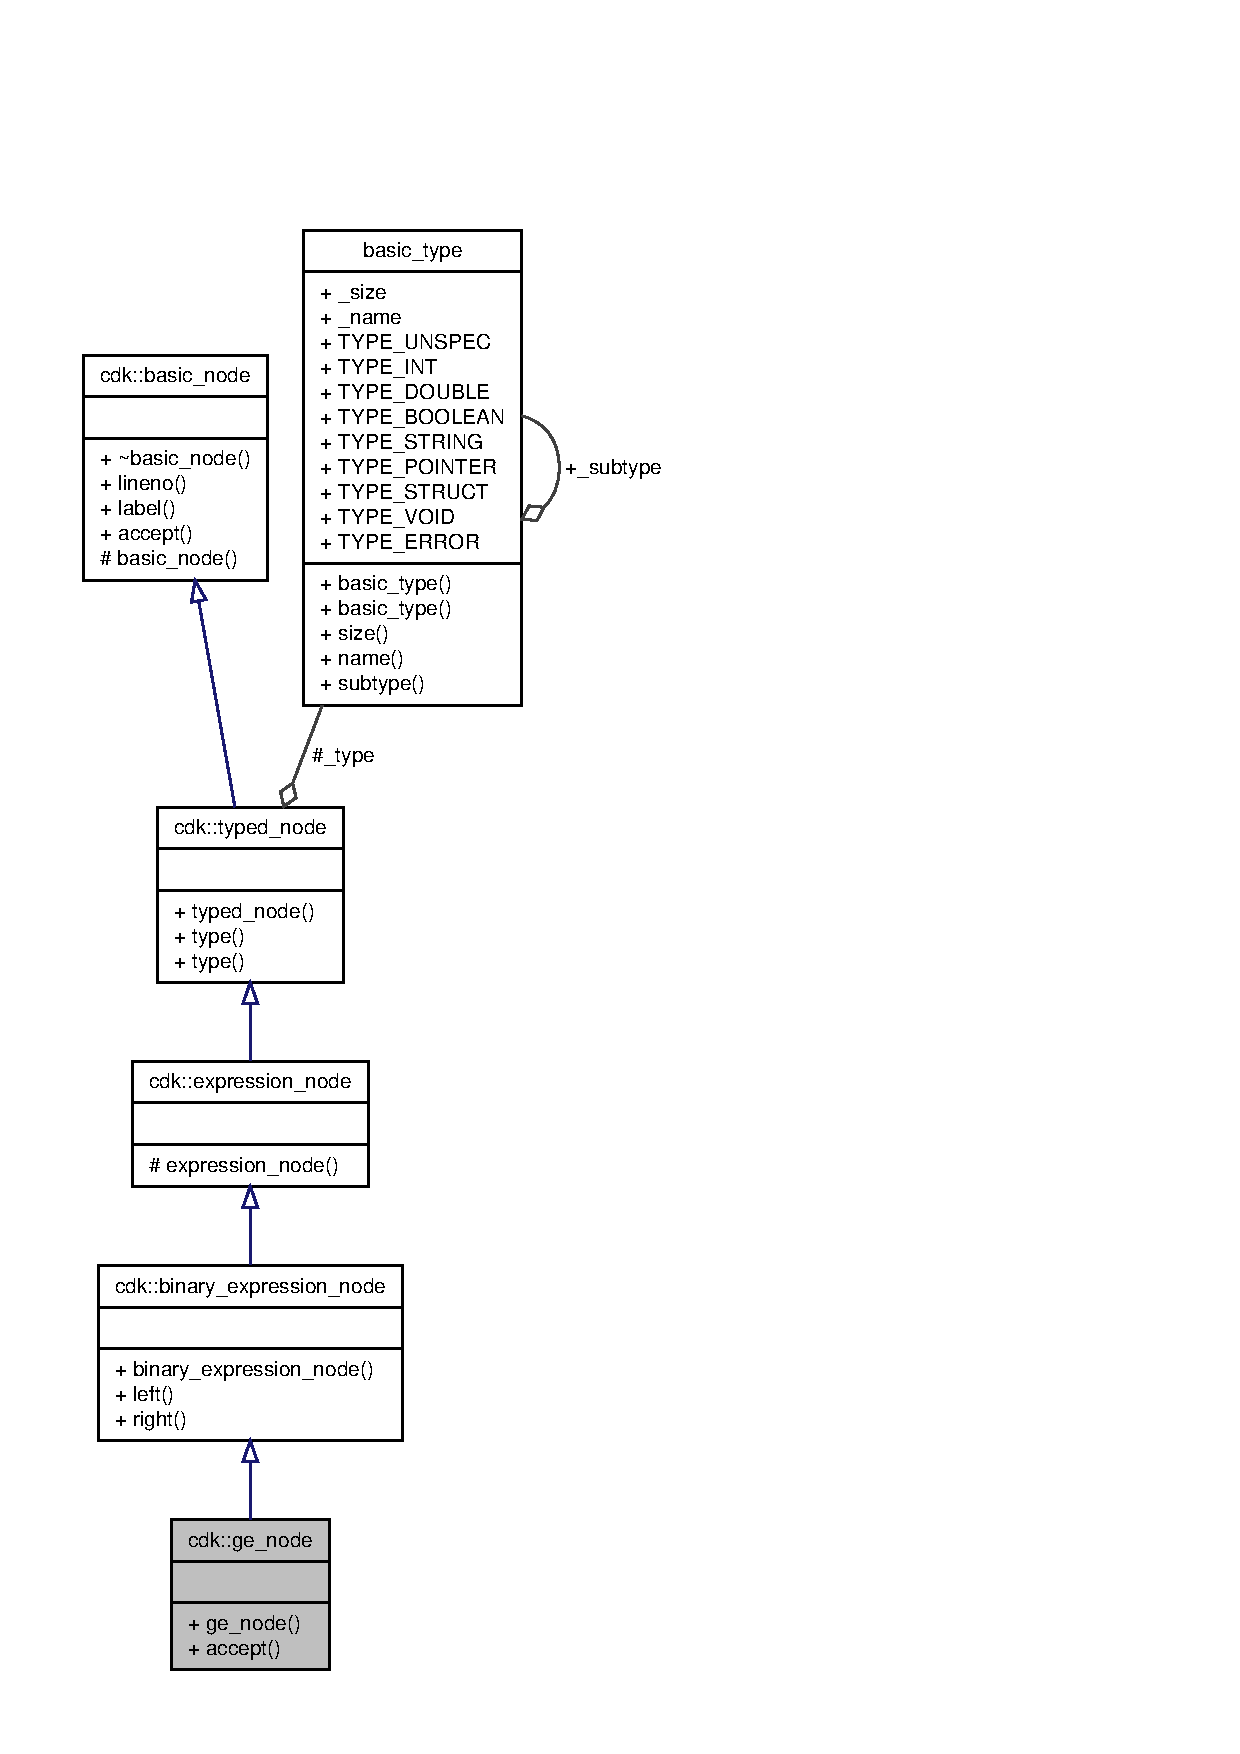
\includegraphics[height=550pt]{classcdk_1_1ge__node__coll__graph}
\end{center}
\end{figure}
\subsection*{Public Member Functions}
\begin{DoxyCompactItemize}
\item 
\textbf{ ge\+\_\+node} (int \textbf{ lineno}, \textbf{ expression\+\_\+node} $\ast$left, \textbf{ expression\+\_\+node} $\ast$right)
\item 
void \textbf{ accept} (\textbf{ basic\+\_\+ast\+\_\+visitor} $\ast$sp, int level)
\end{DoxyCompactItemize}
\subsection*{Additional Inherited Members}


\subsection{Detailed Description}
Class for describing the greater-\/than-\/or-\/equal operator 

Definition at line 11 of file ge\+\_\+node.\+h.



\subsection{Constructor \& Destructor Documentation}
\mbox{\label{classcdk_1_1ge__node_a41b006478853b8f128a381d136a9055f}} 
\index{cdk\+::ge\+\_\+node@{cdk\+::ge\+\_\+node}!ge\+\_\+node@{ge\+\_\+node}}
\index{ge\+\_\+node@{ge\+\_\+node}!cdk\+::ge\+\_\+node@{cdk\+::ge\+\_\+node}}
\subsubsection{ge\+\_\+node()}
{\footnotesize\ttfamily cdk\+::ge\+\_\+node\+::ge\+\_\+node (\begin{DoxyParamCaption}\item[{int}]{lineno,  }\item[{\textbf{ expression\+\_\+node} $\ast$}]{left,  }\item[{\textbf{ expression\+\_\+node} $\ast$}]{right }\end{DoxyParamCaption})\hspace{0.3cm}{\ttfamily [inline]}}


\begin{DoxyParams}{Parameters}
{\em lineno} & source code line number for this node \\
\hline
{\em left} & first operand \\
\hline
{\em right} & second operand \\
\hline
\end{DoxyParams}


Definition at line 18 of file ge\+\_\+node.\+h.



\subsection{Member Function Documentation}
\mbox{\label{classcdk_1_1ge__node_a758ad0281c1e925aab356d757bedce40}} 
\index{cdk\+::ge\+\_\+node@{cdk\+::ge\+\_\+node}!accept@{accept}}
\index{accept@{accept}!cdk\+::ge\+\_\+node@{cdk\+::ge\+\_\+node}}
\subsubsection{accept()}
{\footnotesize\ttfamily void cdk\+::ge\+\_\+node\+::accept (\begin{DoxyParamCaption}\item[{\textbf{ basic\+\_\+ast\+\_\+visitor} $\ast$}]{sp,  }\item[{int}]{level }\end{DoxyParamCaption})\hspace{0.3cm}{\ttfamily [inline]}, {\ttfamily [virtual]}}


\begin{DoxyParams}{Parameters}
{\em sp} & semantic processor visitor \\
\hline
{\em level} & syntactic tree level \\
\hline
\end{DoxyParams}


Implements \textbf{ cdk\+::basic\+\_\+node} \doxyref{}{p.}{classcdk_1_1basic__node_ab38adcbc95c46b809961278afae3bf05}.



Definition at line 26 of file ge\+\_\+node.\+h.



The documentation for this class was generated from the following file\+:\begin{DoxyCompactItemize}
\item 
ast/ge\+\_\+node.\+h\end{DoxyCompactItemize}

\section{cdk\+:\+:gt\+\_\+node Class Reference}
\label{classcdk_1_1gt__node}\index{cdk\+::gt\+\_\+node@{cdk\+::gt\+\_\+node}}


{\ttfamily \#include $<$gt\+\_\+node.\+h$>$}



Inheritance diagram for cdk\+:\+:gt\+\_\+node\+:
\nopagebreak
\begin{figure}[H]
\begin{center}
\leavevmode
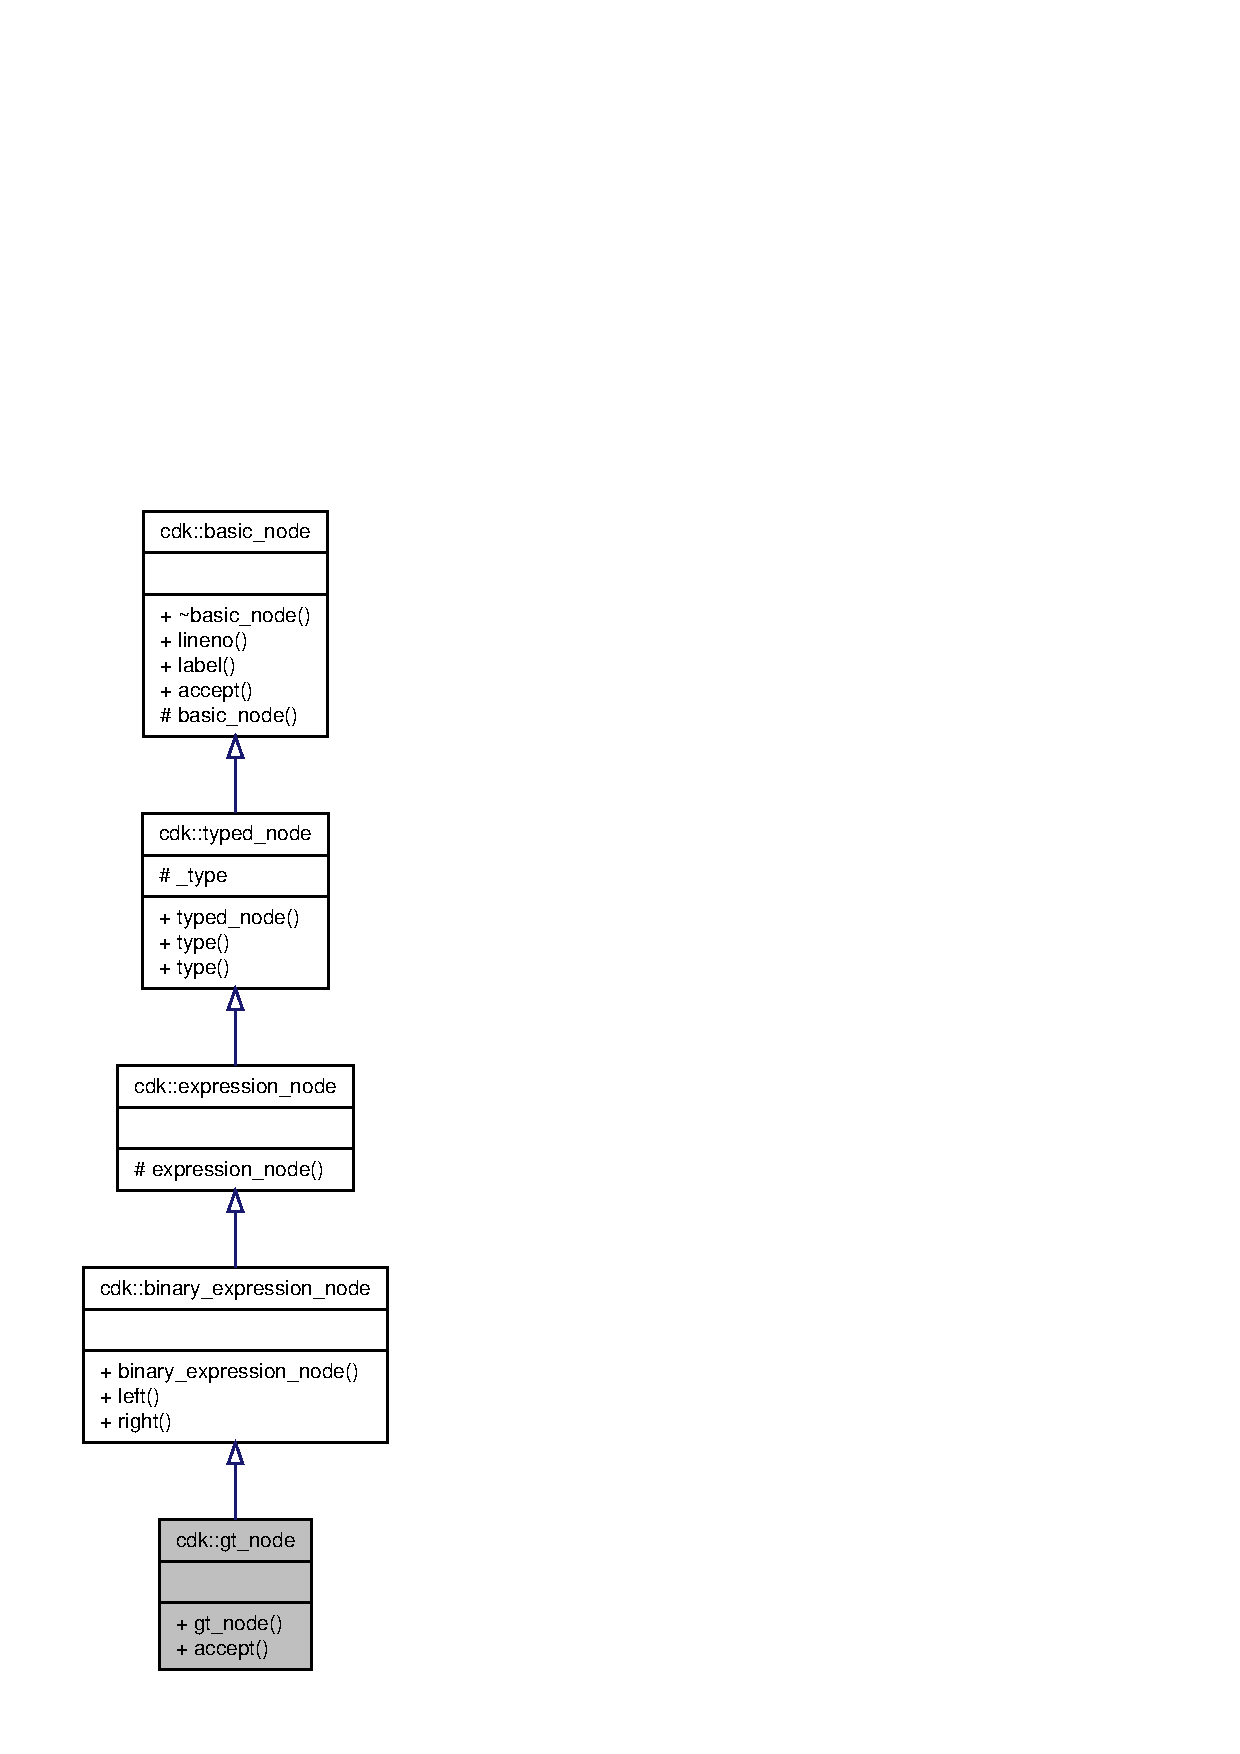
\includegraphics[height=550pt]{classcdk_1_1gt__node__inherit__graph}
\end{center}
\end{figure}


Collaboration diagram for cdk\+:\+:gt\+\_\+node\+:
\nopagebreak
\begin{figure}[H]
\begin{center}
\leavevmode
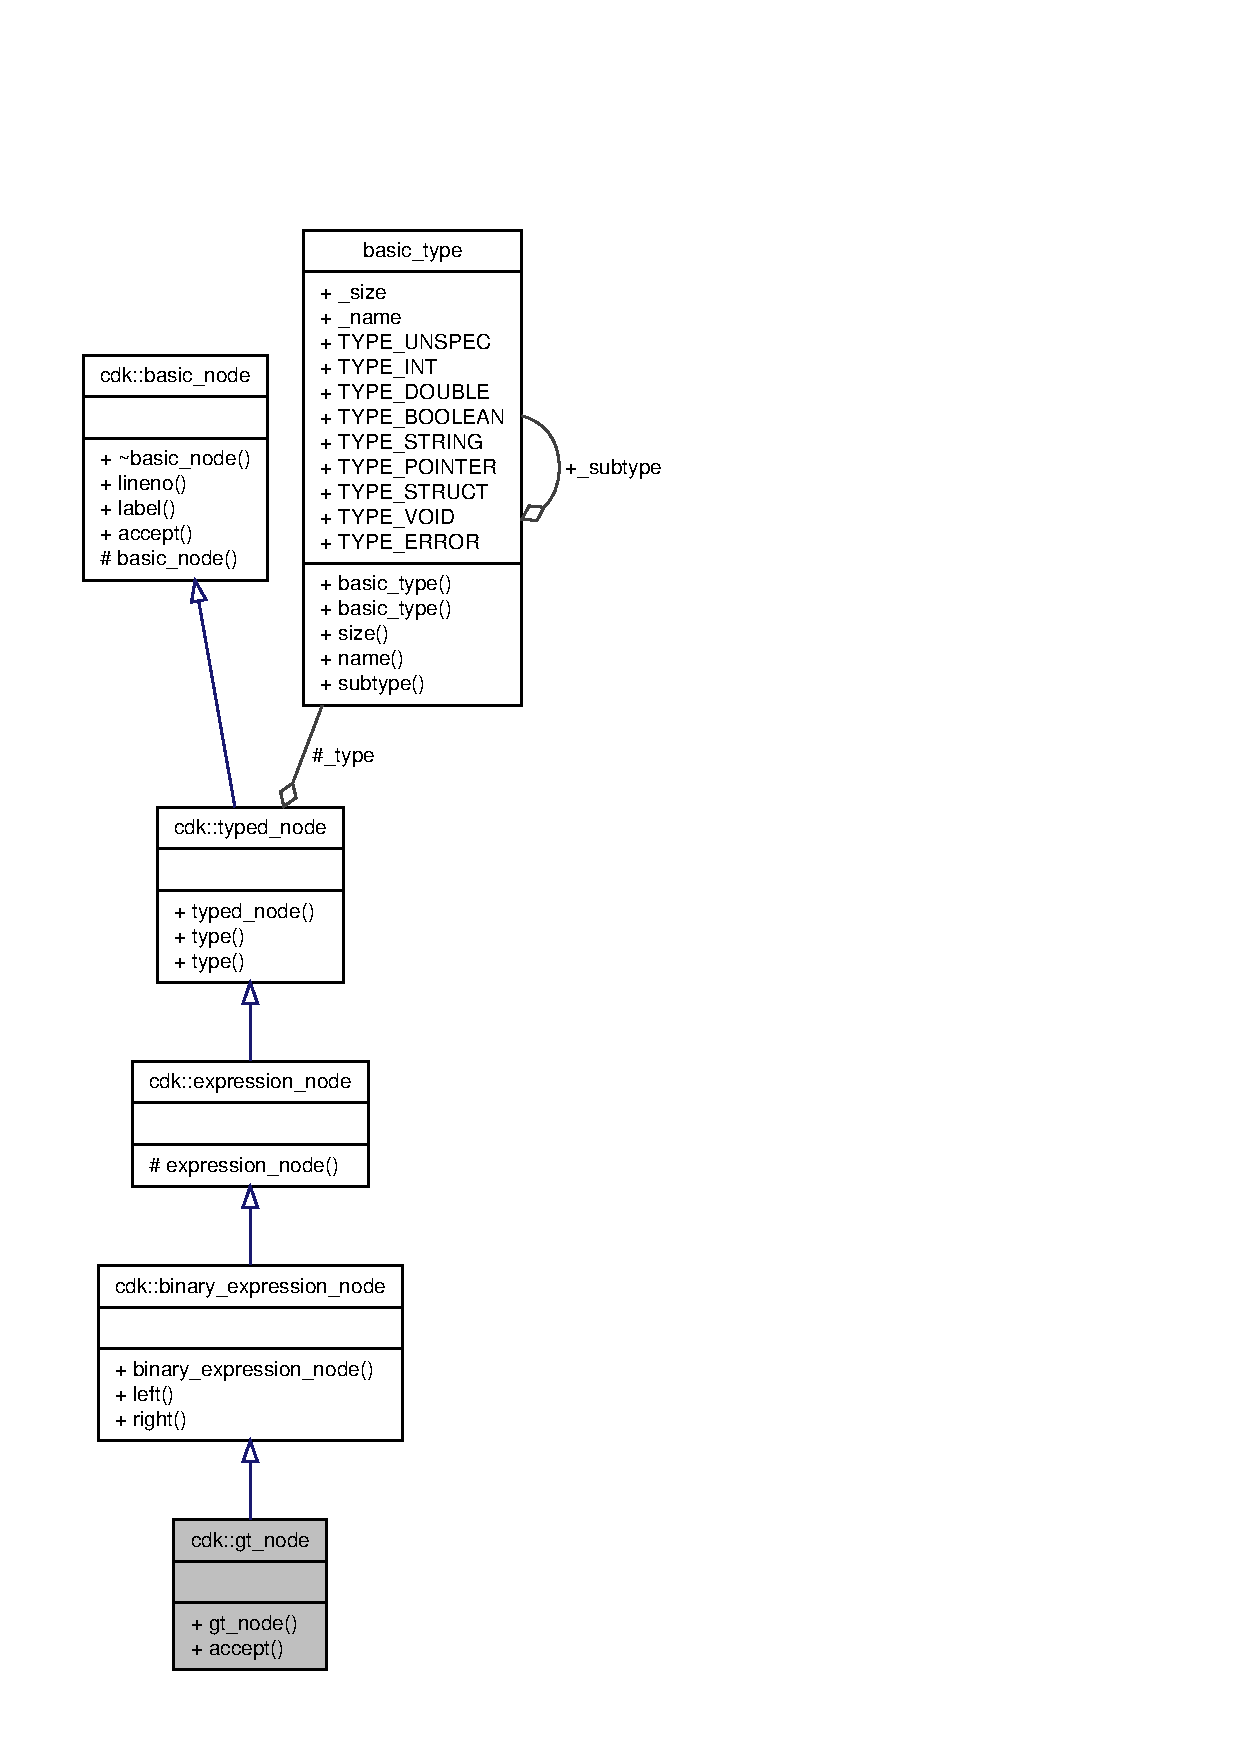
\includegraphics[height=550pt]{classcdk_1_1gt__node__coll__graph}
\end{center}
\end{figure}
\subsection*{Public Member Functions}
\begin{DoxyCompactItemize}
\item 
\textbf{ gt\+\_\+node} (int \textbf{ lineno}, \textbf{ expression\+\_\+node} $\ast$left, \textbf{ expression\+\_\+node} $\ast$right)
\item 
void \textbf{ accept} (\textbf{ basic\+\_\+ast\+\_\+visitor} $\ast$sp, int level)
\end{DoxyCompactItemize}
\subsection*{Additional Inherited Members}


\subsection{Detailed Description}
Class for describing the greater-\/than operator 

Definition at line 11 of file gt\+\_\+node.\+h.



\subsection{Constructor \& Destructor Documentation}
\mbox{\label{classcdk_1_1gt__node_addd29c7a03ecba8714dbb097c856dfd9}} 
\index{cdk\+::gt\+\_\+node@{cdk\+::gt\+\_\+node}!gt\+\_\+node@{gt\+\_\+node}}
\index{gt\+\_\+node@{gt\+\_\+node}!cdk\+::gt\+\_\+node@{cdk\+::gt\+\_\+node}}
\subsubsection{gt\+\_\+node()}
{\footnotesize\ttfamily cdk\+::gt\+\_\+node\+::gt\+\_\+node (\begin{DoxyParamCaption}\item[{int}]{lineno,  }\item[{\textbf{ expression\+\_\+node} $\ast$}]{left,  }\item[{\textbf{ expression\+\_\+node} $\ast$}]{right }\end{DoxyParamCaption})\hspace{0.3cm}{\ttfamily [inline]}}


\begin{DoxyParams}{Parameters}
{\em lineno} & source code line number for this node \\
\hline
{\em left} & first operand \\
\hline
{\em right} & second operand \\
\hline
\end{DoxyParams}


Definition at line 18 of file gt\+\_\+node.\+h.



\subsection{Member Function Documentation}
\mbox{\label{classcdk_1_1gt__node_ab1104710ad583f4b13d397bf33b2f9f5}} 
\index{cdk\+::gt\+\_\+node@{cdk\+::gt\+\_\+node}!accept@{accept}}
\index{accept@{accept}!cdk\+::gt\+\_\+node@{cdk\+::gt\+\_\+node}}
\subsubsection{accept()}
{\footnotesize\ttfamily void cdk\+::gt\+\_\+node\+::accept (\begin{DoxyParamCaption}\item[{\textbf{ basic\+\_\+ast\+\_\+visitor} $\ast$}]{sp,  }\item[{int}]{level }\end{DoxyParamCaption})\hspace{0.3cm}{\ttfamily [inline]}, {\ttfamily [virtual]}}


\begin{DoxyParams}{Parameters}
{\em sp} & semantic processor visitor \\
\hline
{\em level} & syntactic tree level \\
\hline
\end{DoxyParams}


Implements \textbf{ cdk\+::basic\+\_\+node} \doxyref{}{p.}{classcdk_1_1basic__node_ab38adcbc95c46b809961278afae3bf05}.



Definition at line 26 of file gt\+\_\+node.\+h.



The documentation for this class was generated from the following file\+:\begin{DoxyCompactItemize}
\item 
ast/gt\+\_\+node.\+h\end{DoxyCompactItemize}

\section{cdk\+:\+:integer\+\_\+node Class Reference}
\label{classcdk_1_1integer__node}\index{cdk\+::integer\+\_\+node@{cdk\+::integer\+\_\+node}}


{\ttfamily \#include $<$integer\+\_\+node.\+h$>$}



Inheritance diagram for cdk\+:\+:integer\+\_\+node\+:
\nopagebreak
\begin{figure}[H]
\begin{center}
\leavevmode
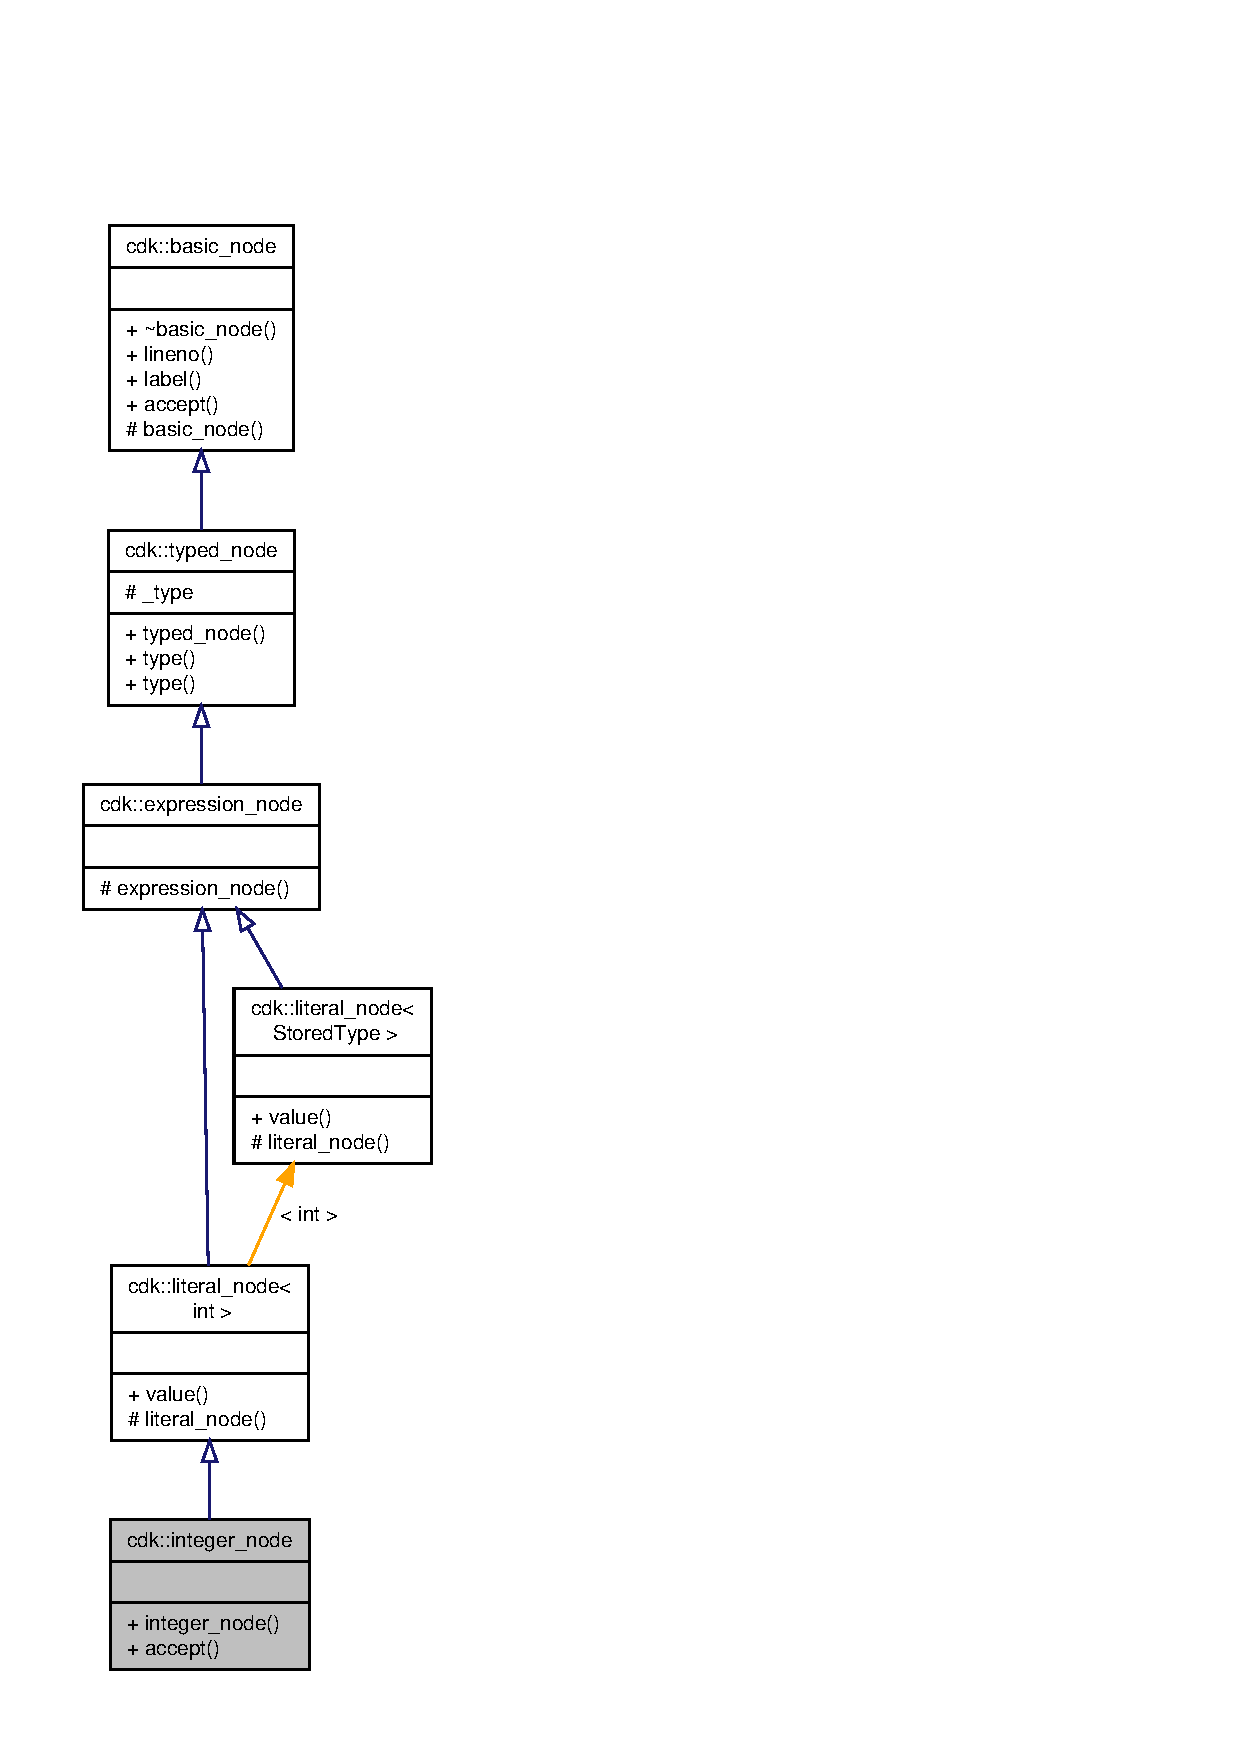
\includegraphics[height=550pt]{classcdk_1_1integer__node__inherit__graph}
\end{center}
\end{figure}


Collaboration diagram for cdk\+:\+:integer\+\_\+node\+:
\nopagebreak
\begin{figure}[H]
\begin{center}
\leavevmode
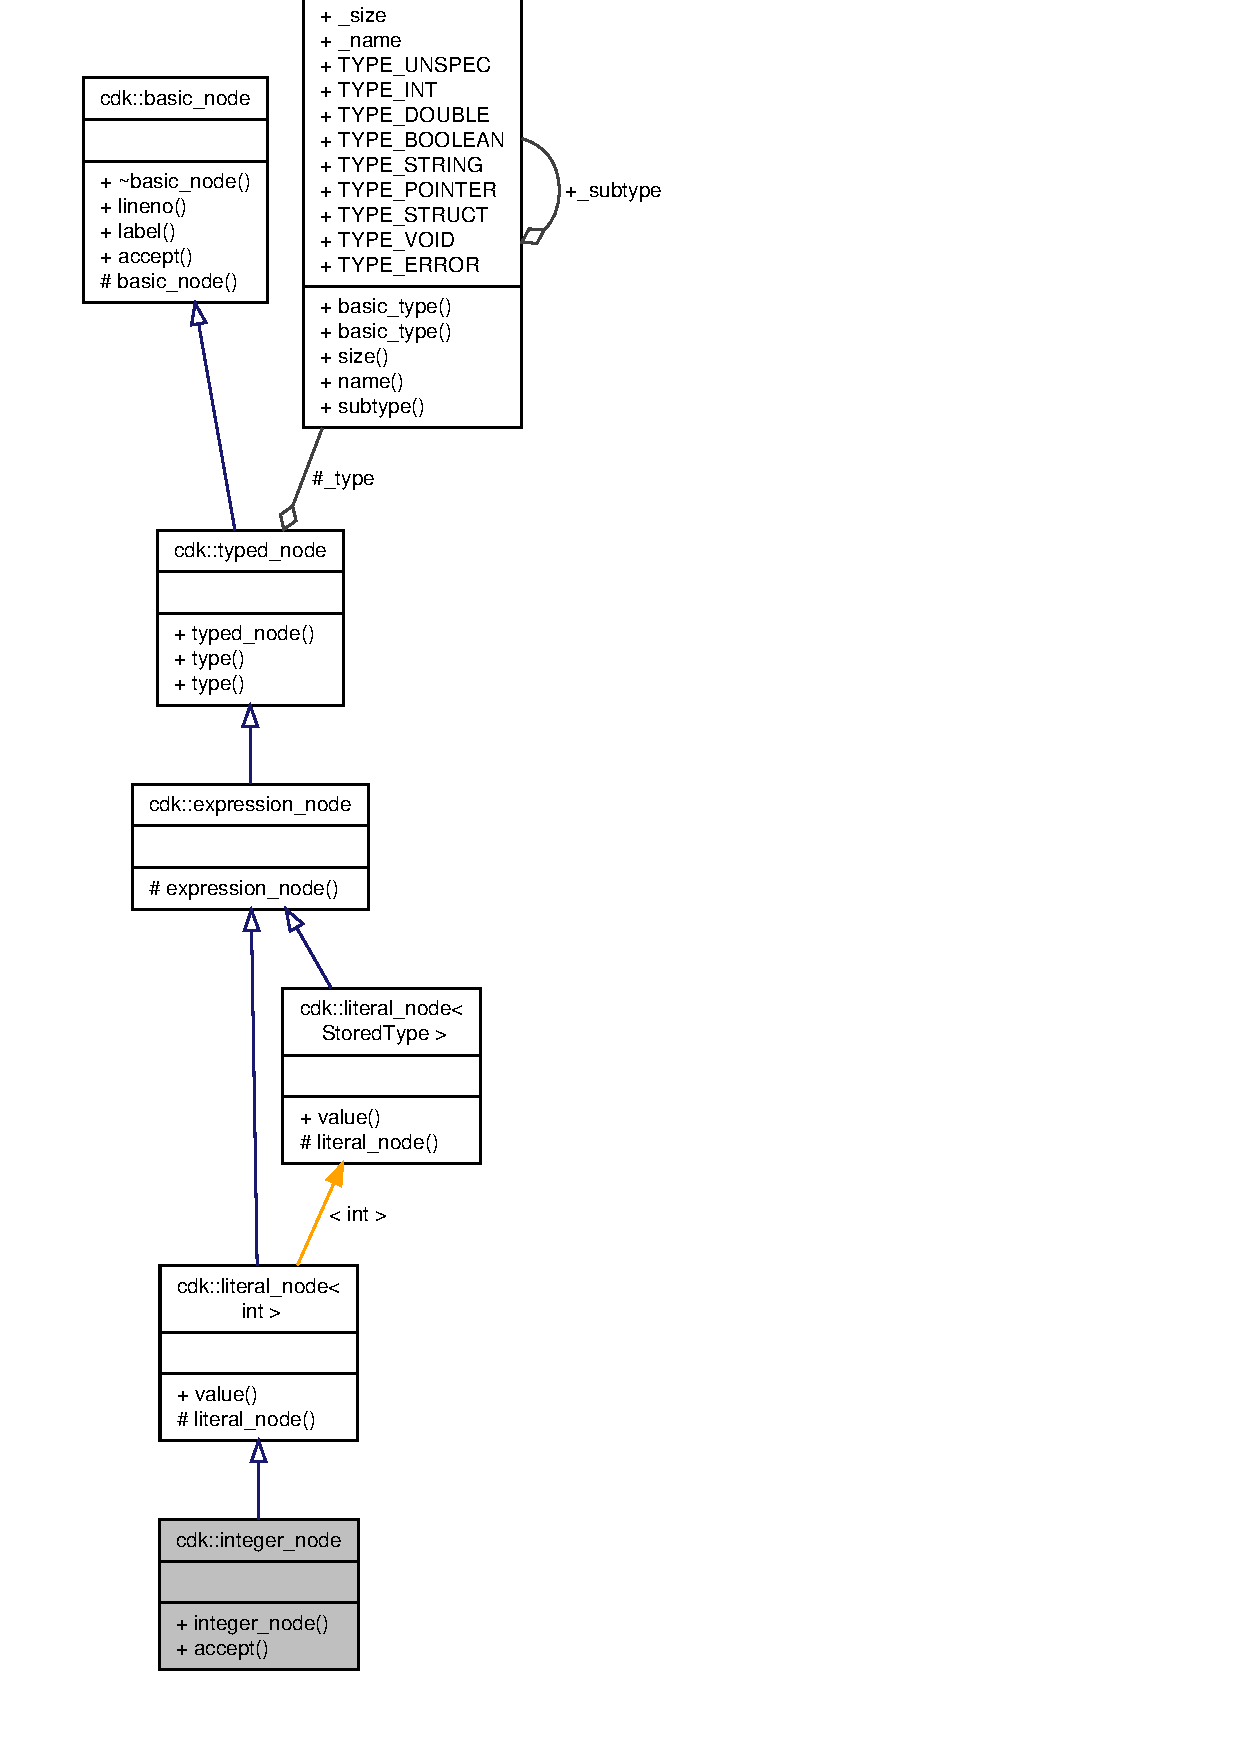
\includegraphics[height=550pt]{classcdk_1_1integer__node__coll__graph}
\end{center}
\end{figure}
\subsection*{Public Member Functions}
\begin{DoxyCompactItemize}
\item 
\mbox{\label{classcdk_1_1integer__node_abb8794adaa28de8eb14f84e3cd3dbfde}} 
{\bfseries integer\+\_\+node} (int \textbf{ lineno}, int i)
\item 
void \textbf{ accept} (\textbf{ basic\+\_\+ast\+\_\+visitor} $\ast$sp, int level)
\end{DoxyCompactItemize}
\subsection*{Additional Inherited Members}


\subsection{Detailed Description}
Class for describing syntactic tree leaves for holding integer values. 

Definition at line 11 of file integer\+\_\+node.\+h.



\subsection{Member Function Documentation}
\mbox{\label{classcdk_1_1integer__node_a6b47d4c572b80bbaed62604a8c68788d}} 
\index{cdk\+::integer\+\_\+node@{cdk\+::integer\+\_\+node}!accept@{accept}}
\index{accept@{accept}!cdk\+::integer\+\_\+node@{cdk\+::integer\+\_\+node}}
\subsubsection{accept()}
{\footnotesize\ttfamily void cdk\+::integer\+\_\+node\+::accept (\begin{DoxyParamCaption}\item[{\textbf{ basic\+\_\+ast\+\_\+visitor} $\ast$}]{sp,  }\item[{int}]{level }\end{DoxyParamCaption})\hspace{0.3cm}{\ttfamily [inline]}, {\ttfamily [virtual]}}


\begin{DoxyParams}{Parameters}
{\em sp} & semantic processor visitor \\
\hline
{\em level} & syntactic tree level \\
\hline
\end{DoxyParams}


Implements \textbf{ cdk\+::basic\+\_\+node} \doxyref{}{p.}{classcdk_1_1basic__node_ab38adcbc95c46b809961278afae3bf05}.



Definition at line 21 of file integer\+\_\+node.\+h.



The documentation for this class was generated from the following file\+:\begin{DoxyCompactItemize}
\item 
ast/integer\+\_\+node.\+h\end{DoxyCompactItemize}

\section{cdk\+:\+:le\+\_\+node Class Reference}
\label{classcdk_1_1le__node}\index{cdk\+::le\+\_\+node@{cdk\+::le\+\_\+node}}


{\ttfamily \#include $<$le\+\_\+node.\+h$>$}



Inheritance diagram for cdk\+:\+:le\+\_\+node\+:
\nopagebreak
\begin{figure}[H]
\begin{center}
\leavevmode
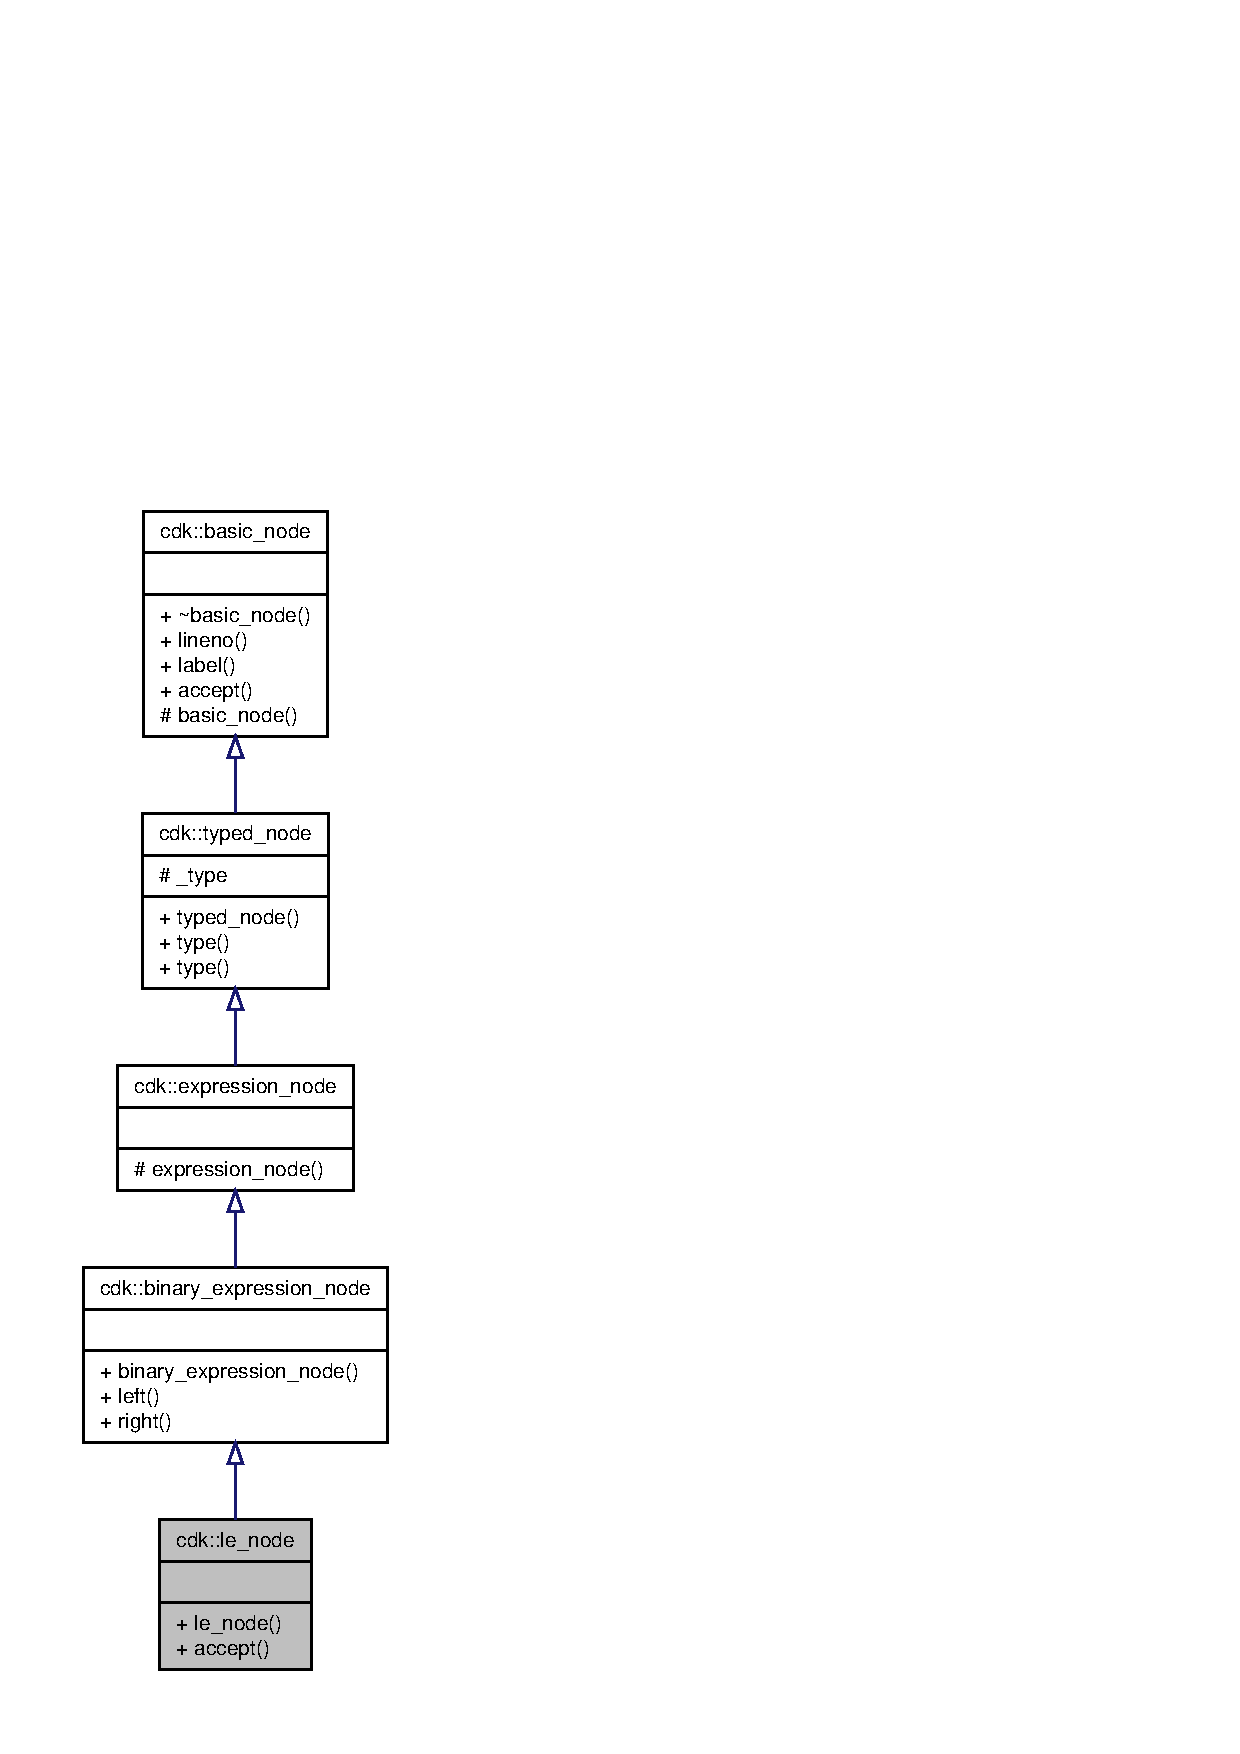
\includegraphics[height=550pt]{classcdk_1_1le__node__inherit__graph}
\end{center}
\end{figure}


Collaboration diagram for cdk\+:\+:le\+\_\+node\+:
\nopagebreak
\begin{figure}[H]
\begin{center}
\leavevmode
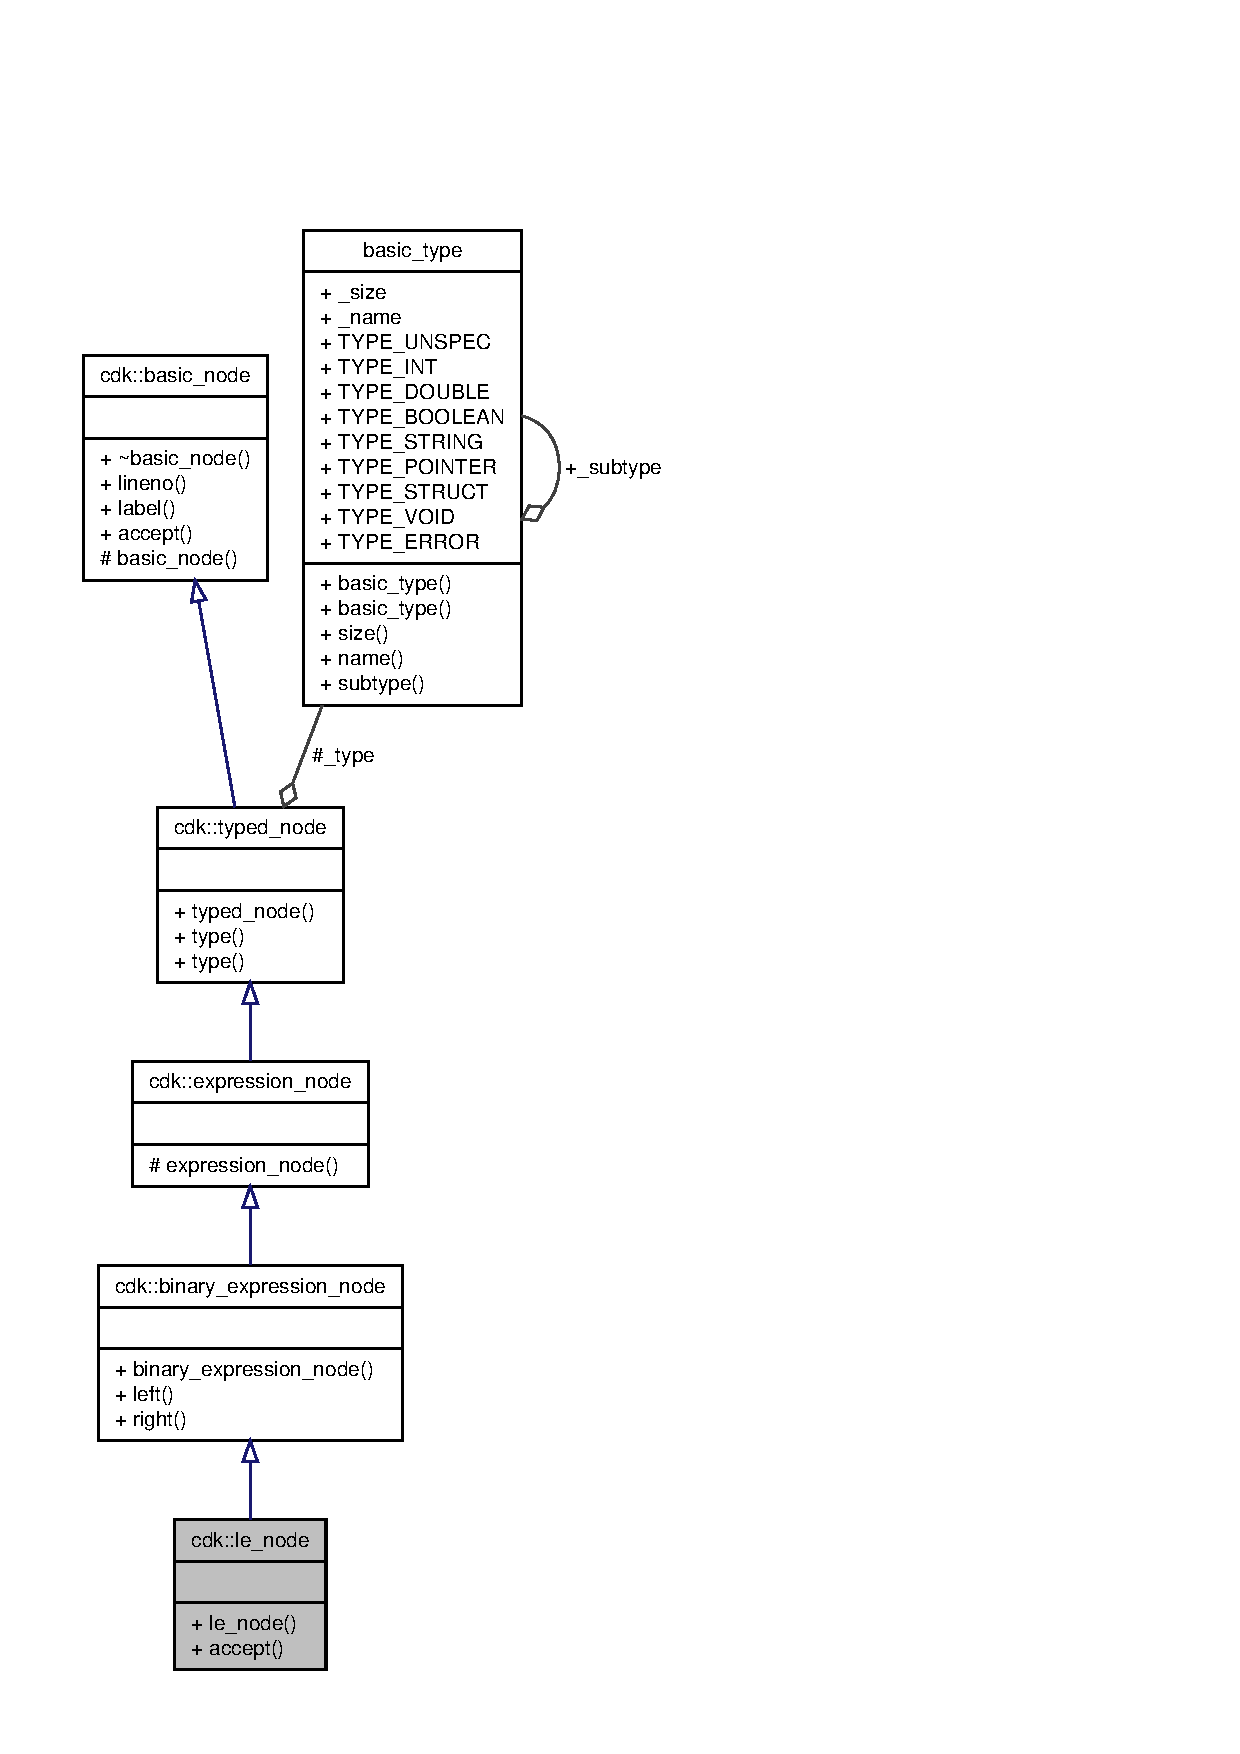
\includegraphics[height=550pt]{classcdk_1_1le__node__coll__graph}
\end{center}
\end{figure}
\subsection*{Public Member Functions}
\begin{DoxyCompactItemize}
\item 
\textbf{ le\+\_\+node} (int \textbf{ lineno}, \textbf{ expression\+\_\+node} $\ast$left, \textbf{ expression\+\_\+node} $\ast$right)
\item 
void \textbf{ accept} (\textbf{ basic\+\_\+ast\+\_\+visitor} $\ast$sp, int level)
\end{DoxyCompactItemize}
\subsection*{Additional Inherited Members}


\subsection{Detailed Description}
Class for describing the lower-\/than-\/or-\/equal operator 

Definition at line 11 of file le\+\_\+node.\+h.



\subsection{Constructor \& Destructor Documentation}
\mbox{\label{classcdk_1_1le__node_a2582bc8b99e25493ad4646156c3bed2d}} 
\index{cdk\+::le\+\_\+node@{cdk\+::le\+\_\+node}!le\+\_\+node@{le\+\_\+node}}
\index{le\+\_\+node@{le\+\_\+node}!cdk\+::le\+\_\+node@{cdk\+::le\+\_\+node}}
\subsubsection{le\+\_\+node()}
{\footnotesize\ttfamily cdk\+::le\+\_\+node\+::le\+\_\+node (\begin{DoxyParamCaption}\item[{int}]{lineno,  }\item[{\textbf{ expression\+\_\+node} $\ast$}]{left,  }\item[{\textbf{ expression\+\_\+node} $\ast$}]{right }\end{DoxyParamCaption})\hspace{0.3cm}{\ttfamily [inline]}}


\begin{DoxyParams}{Parameters}
{\em lineno} & source code line number for this node \\
\hline
{\em left} & first operand \\
\hline
{\em right} & second operand \\
\hline
\end{DoxyParams}


Definition at line 18 of file le\+\_\+node.\+h.



\subsection{Member Function Documentation}
\mbox{\label{classcdk_1_1le__node_a4d3a01246f47dcb95ab7535a9047c9d6}} 
\index{cdk\+::le\+\_\+node@{cdk\+::le\+\_\+node}!accept@{accept}}
\index{accept@{accept}!cdk\+::le\+\_\+node@{cdk\+::le\+\_\+node}}
\subsubsection{accept()}
{\footnotesize\ttfamily void cdk\+::le\+\_\+node\+::accept (\begin{DoxyParamCaption}\item[{\textbf{ basic\+\_\+ast\+\_\+visitor} $\ast$}]{sp,  }\item[{int}]{level }\end{DoxyParamCaption})\hspace{0.3cm}{\ttfamily [inline]}, {\ttfamily [virtual]}}


\begin{DoxyParams}{Parameters}
{\em sp} & semantic processor visitor \\
\hline
{\em level} & syntactic tree level \\
\hline
\end{DoxyParams}


Implements \textbf{ cdk\+::basic\+\_\+node} \doxyref{}{p.}{classcdk_1_1basic__node_ab38adcbc95c46b809961278afae3bf05}.



Definition at line 26 of file le\+\_\+node.\+h.



The documentation for this class was generated from the following file\+:\begin{DoxyCompactItemize}
\item 
ast/le\+\_\+node.\+h\end{DoxyCompactItemize}

\section{cdk\+:\+:literal\+\_\+node$<$ Stored\+Type $>$ Class Template Reference}
\label{classcdk_1_1literal__node}\index{cdk\+::literal\+\_\+node$<$ Stored\+Type $>$@{cdk\+::literal\+\_\+node$<$ Stored\+Type $>$}}


{\ttfamily \#include $<$literal\+\_\+node.\+h$>$}



Inheritance diagram for cdk\+:\+:literal\+\_\+node$<$ Stored\+Type $>$\+:
\nopagebreak
\begin{figure}[H]
\begin{center}
\leavevmode
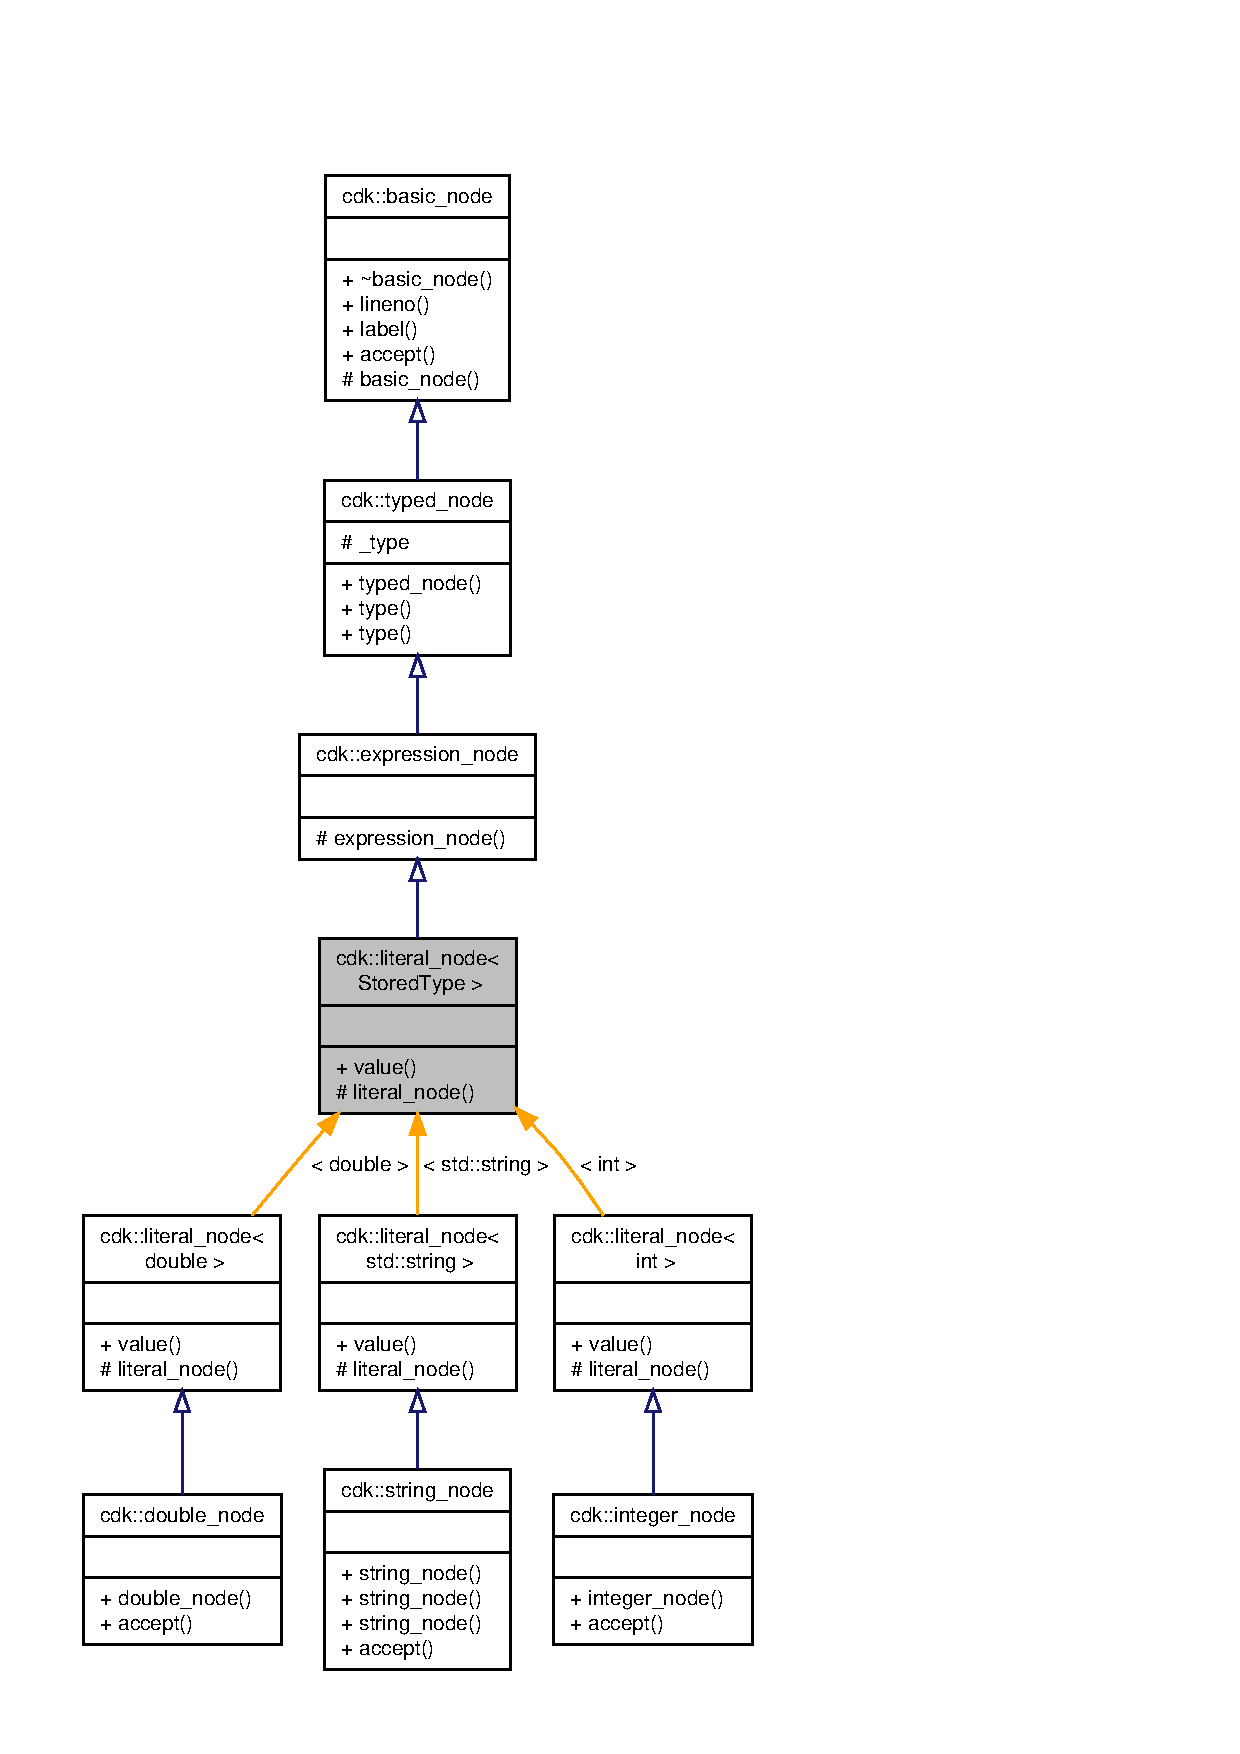
\includegraphics[height=550pt]{classcdk_1_1literal__node__inherit__graph}
\end{center}
\end{figure}


Collaboration diagram for cdk\+:\+:literal\+\_\+node$<$ Stored\+Type $>$\+:
\nopagebreak
\begin{figure}[H]
\begin{center}
\leavevmode
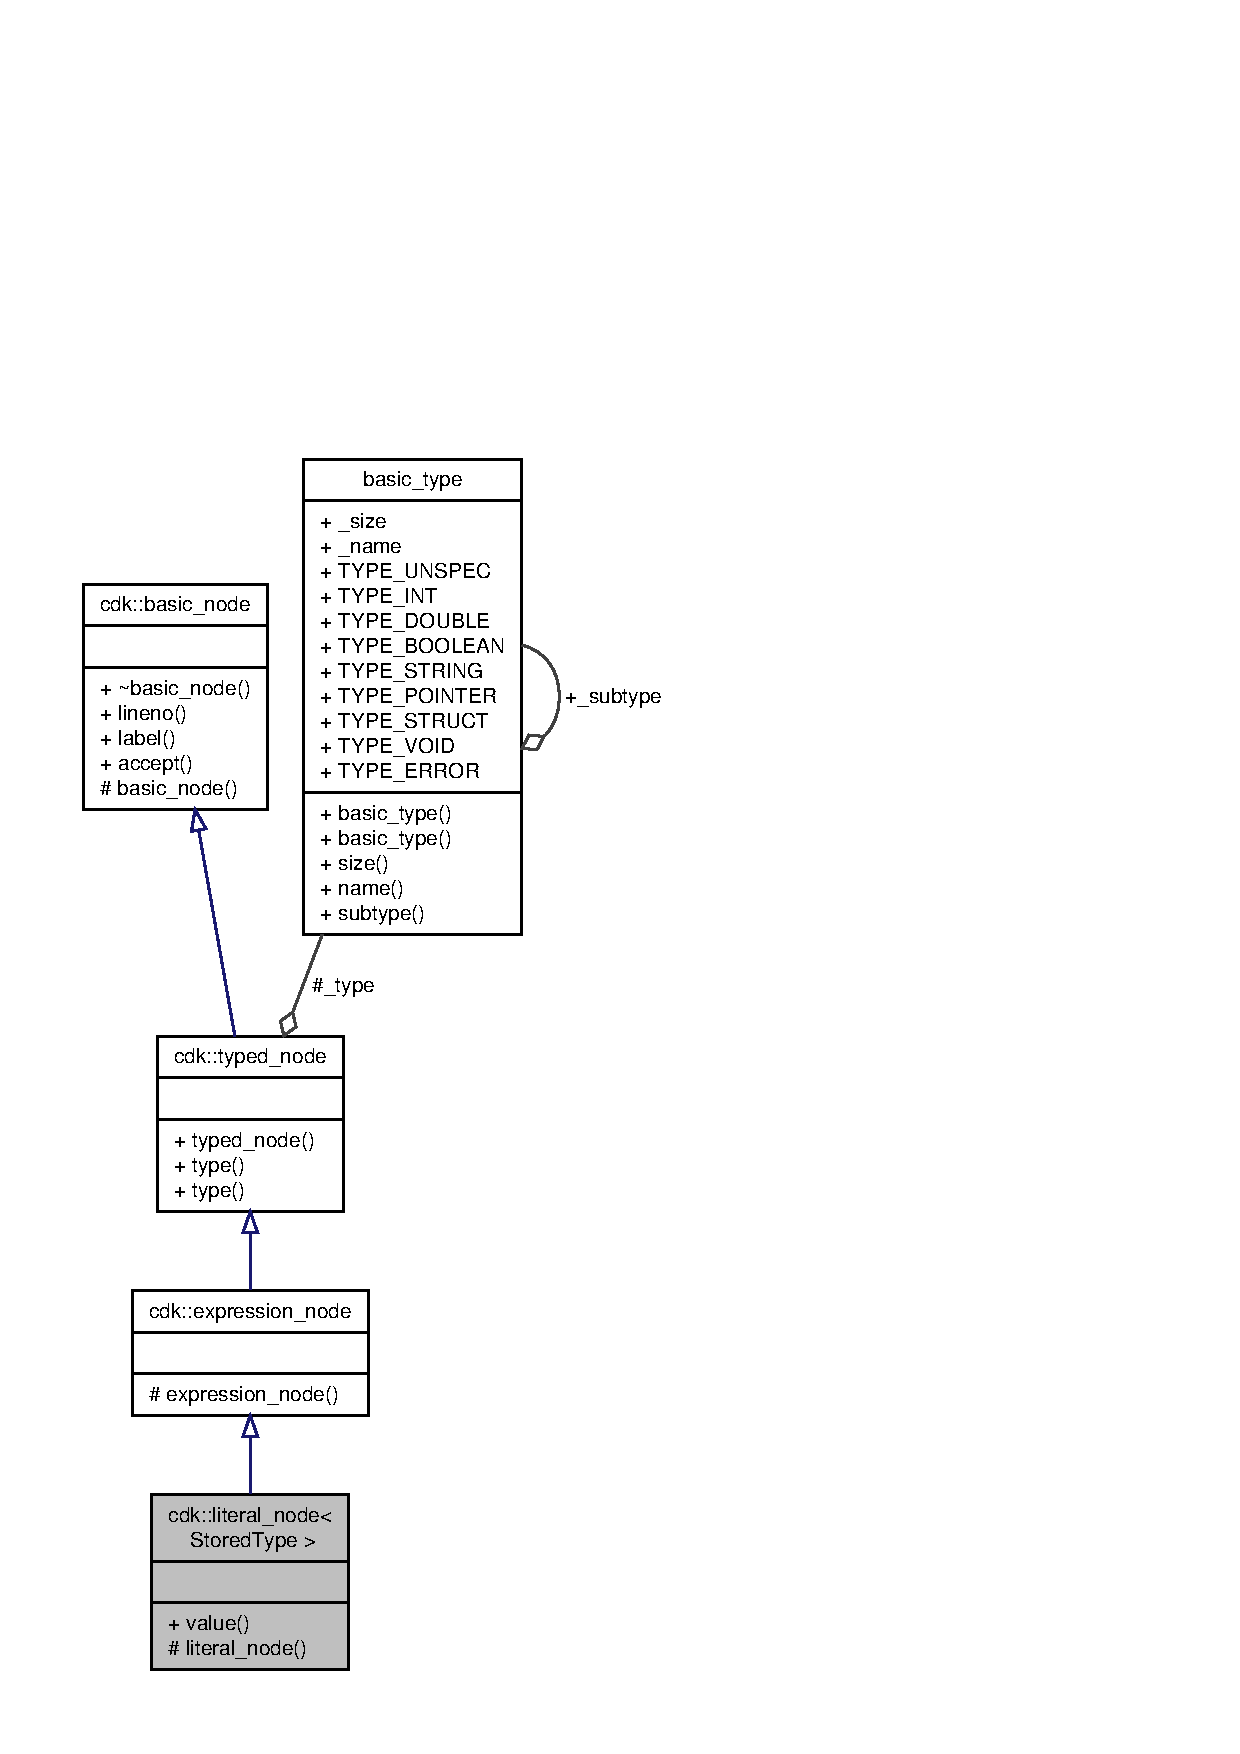
\includegraphics[height=550pt]{classcdk_1_1literal__node__coll__graph}
\end{center}
\end{figure}
\subsection*{Public Member Functions}
\begin{DoxyCompactItemize}
\item 
\mbox{\label{classcdk_1_1literal__node_a2285a40a719019c68a379950ddc9ffc9}} 
const Stored\+Type \& {\bfseries value} () const
\end{DoxyCompactItemize}
\subsection*{Protected Member Functions}
\begin{DoxyCompactItemize}
\item 
\mbox{\label{classcdk_1_1literal__node_aa75409de8595d4073ca995f988210ae8}} 
{\bfseries literal\+\_\+node} (int \textbf{ lineno}, const Stored\+Type \&value)
\end{DoxyCompactItemize}
\subsection*{Additional Inherited Members}


\subsection{Detailed Description}
\subsubsection*{template$<$typename Stored\+Type$>$\newline
class cdk\+::literal\+\_\+node$<$ Stored\+Type $>$}

Class for describing syntactic tree leaves for holding literal nodes. This is a template class that will be instantiated by the various classes for holding specific leaves.


\begin{DoxyParams}{Parameters}
{\em Stored\+Type} & is the type held by the leaf \\
\hline
\end{DoxyParams}
\begin{DoxySeeAlso}{See also}
Double, Integer, String 
\end{DoxySeeAlso}


Definition at line 17 of file literal\+\_\+node.\+h.



The documentation for this class was generated from the following file\+:\begin{DoxyCompactItemize}
\item 
ast/literal\+\_\+node.\+h\end{DoxyCompactItemize}

\section{cdk\+:\+:lt\+\_\+node Class Reference}
\label{classcdk_1_1lt__node}\index{cdk\+::lt\+\_\+node@{cdk\+::lt\+\_\+node}}


{\ttfamily \#include $<$lt\+\_\+node.\+h$>$}



Inheritance diagram for cdk\+:\+:lt\+\_\+node\+:
\nopagebreak
\begin{figure}[H]
\begin{center}
\leavevmode
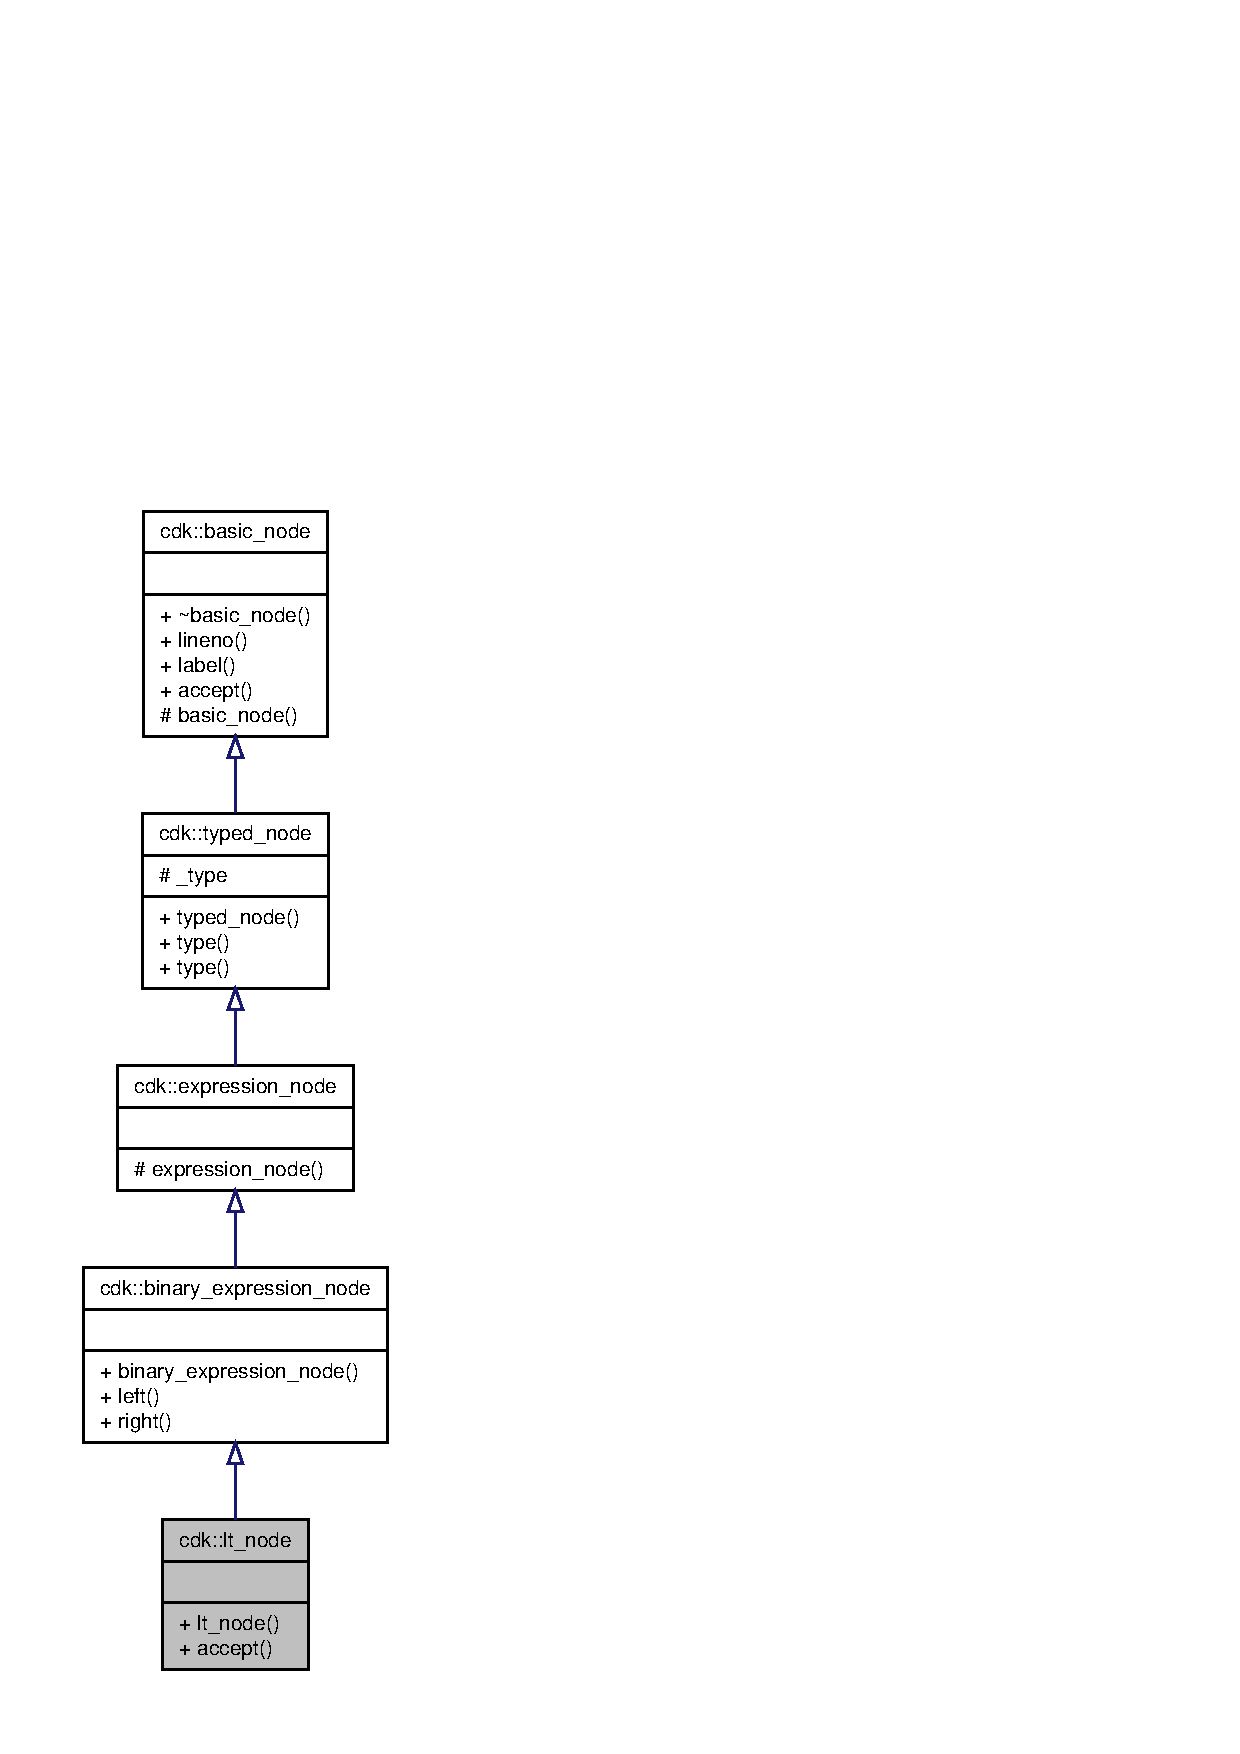
\includegraphics[height=550pt]{classcdk_1_1lt__node__inherit__graph}
\end{center}
\end{figure}


Collaboration diagram for cdk\+:\+:lt\+\_\+node\+:
\nopagebreak
\begin{figure}[H]
\begin{center}
\leavevmode
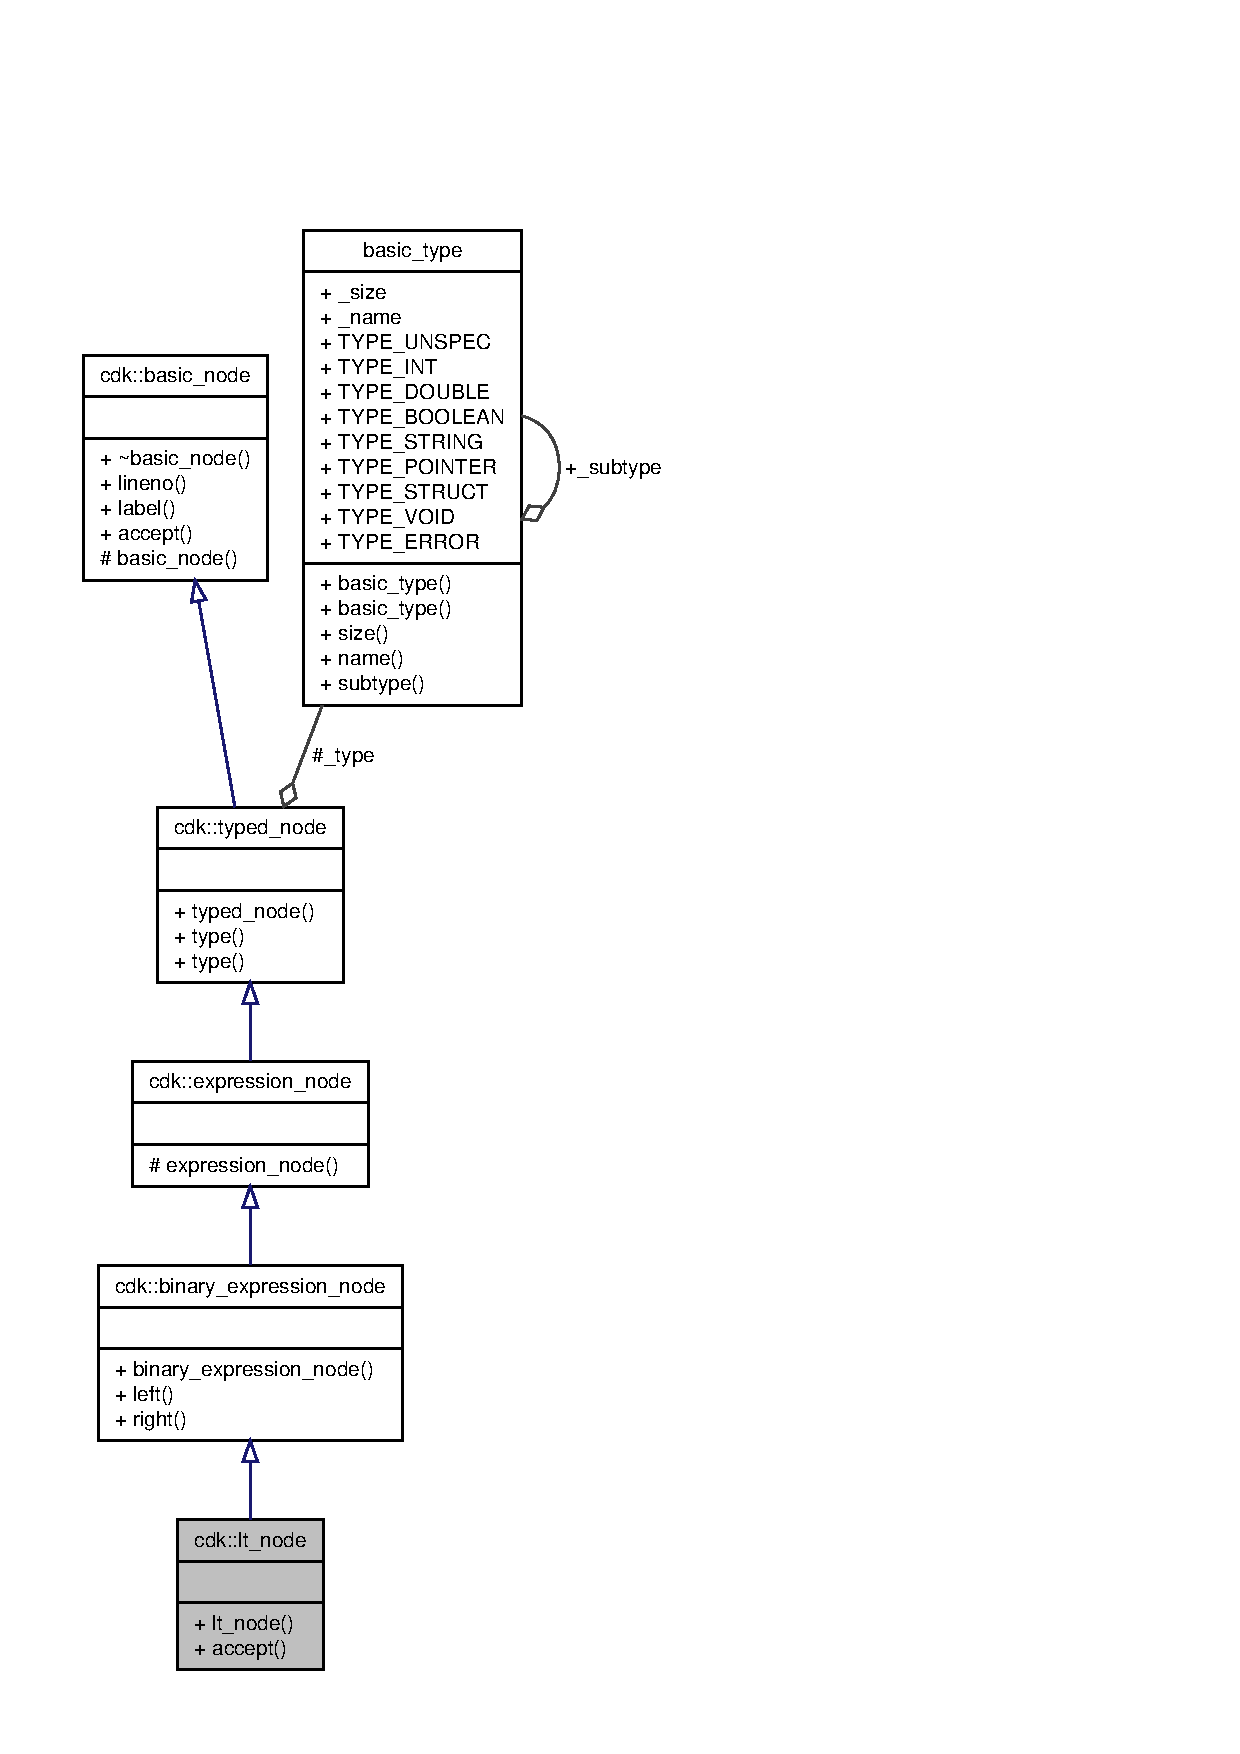
\includegraphics[height=550pt]{classcdk_1_1lt__node__coll__graph}
\end{center}
\end{figure}
\subsection*{Public Member Functions}
\begin{DoxyCompactItemize}
\item 
\textbf{ lt\+\_\+node} (int \textbf{ lineno}, \textbf{ expression\+\_\+node} $\ast$left, \textbf{ expression\+\_\+node} $\ast$right)
\item 
void \textbf{ accept} (\textbf{ basic\+\_\+ast\+\_\+visitor} $\ast$sp, int level)
\end{DoxyCompactItemize}
\subsection*{Additional Inherited Members}


\subsection{Detailed Description}
Class for describing the lower-\/than operator 

Definition at line 11 of file lt\+\_\+node.\+h.



\subsection{Constructor \& Destructor Documentation}
\mbox{\label{classcdk_1_1lt__node_a2c3e8e72fb6385cc25ea2bc3cd594bc5}} 
\index{cdk\+::lt\+\_\+node@{cdk\+::lt\+\_\+node}!lt\+\_\+node@{lt\+\_\+node}}
\index{lt\+\_\+node@{lt\+\_\+node}!cdk\+::lt\+\_\+node@{cdk\+::lt\+\_\+node}}
\subsubsection{lt\+\_\+node()}
{\footnotesize\ttfamily cdk\+::lt\+\_\+node\+::lt\+\_\+node (\begin{DoxyParamCaption}\item[{int}]{lineno,  }\item[{\textbf{ expression\+\_\+node} $\ast$}]{left,  }\item[{\textbf{ expression\+\_\+node} $\ast$}]{right }\end{DoxyParamCaption})\hspace{0.3cm}{\ttfamily [inline]}}


\begin{DoxyParams}{Parameters}
{\em lineno} & source code line number for this node \\
\hline
{\em left} & first operand \\
\hline
{\em right} & second operand \\
\hline
\end{DoxyParams}


Definition at line 18 of file lt\+\_\+node.\+h.



\subsection{Member Function Documentation}
\mbox{\label{classcdk_1_1lt__node_a6af8ca3130c12e7a38860c9e92aaaa97}} 
\index{cdk\+::lt\+\_\+node@{cdk\+::lt\+\_\+node}!accept@{accept}}
\index{accept@{accept}!cdk\+::lt\+\_\+node@{cdk\+::lt\+\_\+node}}
\subsubsection{accept()}
{\footnotesize\ttfamily void cdk\+::lt\+\_\+node\+::accept (\begin{DoxyParamCaption}\item[{\textbf{ basic\+\_\+ast\+\_\+visitor} $\ast$}]{sp,  }\item[{int}]{level }\end{DoxyParamCaption})\hspace{0.3cm}{\ttfamily [inline]}, {\ttfamily [virtual]}}


\begin{DoxyParams}{Parameters}
{\em sp} & semantic processor visitor \\
\hline
{\em level} & syntactic tree level \\
\hline
\end{DoxyParams}


Implements \textbf{ cdk\+::basic\+\_\+node} \doxyref{}{p.}{classcdk_1_1basic__node_ab38adcbc95c46b809961278afae3bf05}.



Definition at line 26 of file lt\+\_\+node.\+h.



The documentation for this class was generated from the following file\+:\begin{DoxyCompactItemize}
\item 
ast/lt\+\_\+node.\+h\end{DoxyCompactItemize}

\section{cdk\+:\+:lvalue\+\_\+node Class Reference}
\label{classcdk_1_1lvalue__node}\index{cdk\+::lvalue\+\_\+node@{cdk\+::lvalue\+\_\+node}}


{\ttfamily \#include $<$lvalue\+\_\+node.\+h$>$}



Inheritance diagram for cdk\+:\+:lvalue\+\_\+node\+:
\nopagebreak
\begin{figure}[H]
\begin{center}
\leavevmode
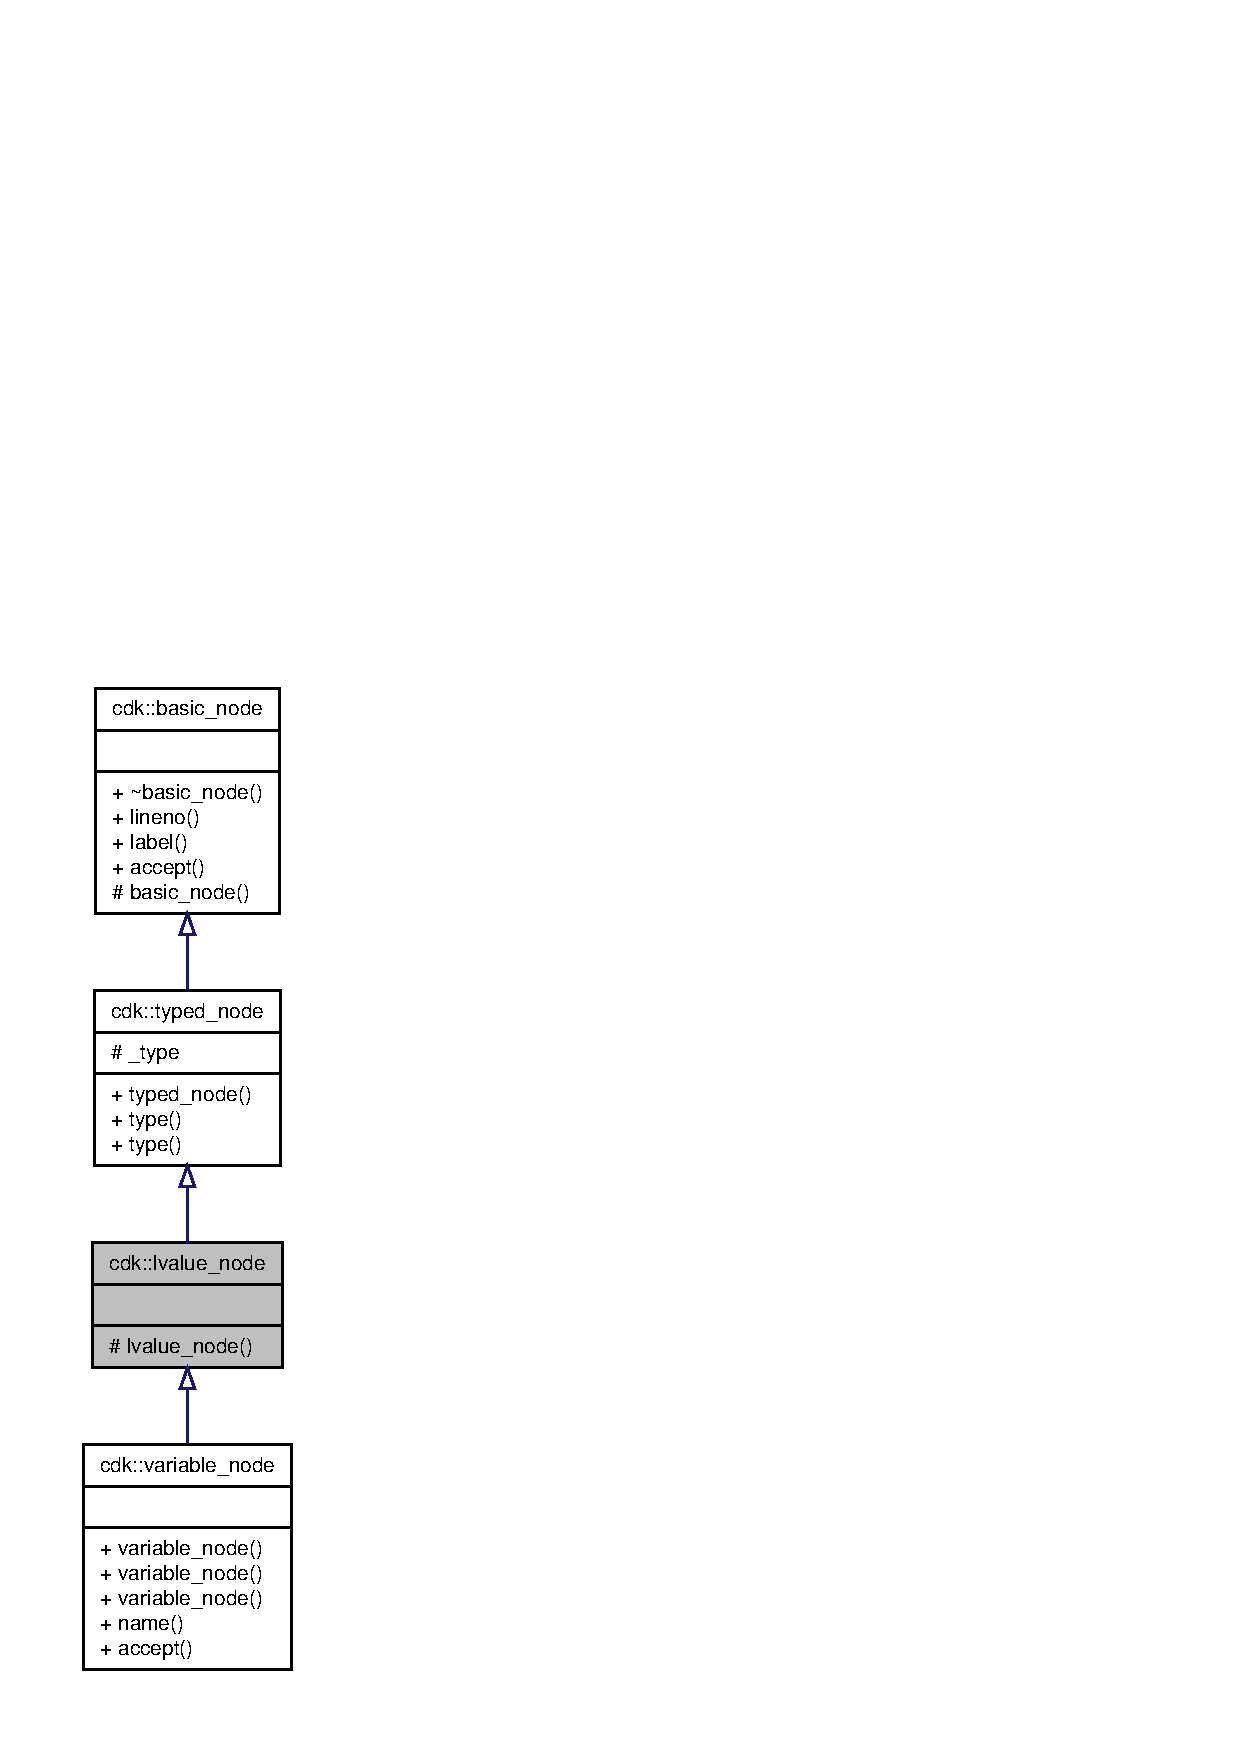
\includegraphics[width=144pt]{classcdk_1_1lvalue__node__inherit__graph}
\end{center}
\end{figure}


Collaboration diagram for cdk\+:\+:lvalue\+\_\+node\+:
\nopagebreak
\begin{figure}[H]
\begin{center}
\leavevmode
\includegraphics[width=322pt]{classcdk_1_1lvalue__node__coll__graph}
\end{center}
\end{figure}
\subsection*{Protected Member Functions}
\begin{DoxyCompactItemize}
\item 
\mbox{\label{classcdk_1_1lvalue__node_ae3f2020c806be939a87f9ae973030a0b}} 
{\bfseries lvalue\+\_\+node} (int \textbf{ lineno})
\end{DoxyCompactItemize}
\subsection*{Additional Inherited Members}


\subsection{Detailed Description}
Class for describing syntactic tree leaves for lvalues. 

Definition at line 12 of file lvalue\+\_\+node.\+h.



The documentation for this class was generated from the following file\+:\begin{DoxyCompactItemize}
\item 
ast/lvalue\+\_\+node.\+h\end{DoxyCompactItemize}

\section{cdk\+:\+:mod\+\_\+node Class Reference}
\label{classcdk_1_1mod__node}\index{cdk\+::mod\+\_\+node@{cdk\+::mod\+\_\+node}}


{\ttfamily \#include $<$mod\+\_\+node.\+h$>$}



Inheritance diagram for cdk\+:\+:mod\+\_\+node\+:
\nopagebreak
\begin{figure}[H]
\begin{center}
\leavevmode
\includegraphics[height=550pt]{classcdk_1_1mod__node__inherit__graph}
\end{center}
\end{figure}


Collaboration diagram for cdk\+:\+:mod\+\_\+node\+:
\nopagebreak
\begin{figure}[H]
\begin{center}
\leavevmode
\includegraphics[height=550pt]{classcdk_1_1mod__node__coll__graph}
\end{center}
\end{figure}
\subsection*{Public Member Functions}
\begin{DoxyCompactItemize}
\item 
\textbf{ mod\+\_\+node} (int \textbf{ lineno}, \textbf{ expression\+\_\+node} $\ast$left, \textbf{ expression\+\_\+node} $\ast$right)
\item 
void \textbf{ accept} (\textbf{ basic\+\_\+ast\+\_\+visitor} $\ast$sp, int level)
\end{DoxyCompactItemize}
\subsection*{Additional Inherited Members}


\subsection{Detailed Description}
Class for describing the modulus operator 

Definition at line 11 of file mod\+\_\+node.\+h.



\subsection{Constructor \& Destructor Documentation}
\mbox{\label{classcdk_1_1mod__node_a1c91715c67e3c28da9cfaeee494d5ad2}} 
\index{cdk\+::mod\+\_\+node@{cdk\+::mod\+\_\+node}!mod\+\_\+node@{mod\+\_\+node}}
\index{mod\+\_\+node@{mod\+\_\+node}!cdk\+::mod\+\_\+node@{cdk\+::mod\+\_\+node}}
\subsubsection{mod\+\_\+node()}
{\footnotesize\ttfamily cdk\+::mod\+\_\+node\+::mod\+\_\+node (\begin{DoxyParamCaption}\item[{int}]{lineno,  }\item[{\textbf{ expression\+\_\+node} $\ast$}]{left,  }\item[{\textbf{ expression\+\_\+node} $\ast$}]{right }\end{DoxyParamCaption})\hspace{0.3cm}{\ttfamily [inline]}}


\begin{DoxyParams}{Parameters}
{\em lineno} & source code line number for this node \\
\hline
{\em left} & first operand \\
\hline
{\em right} & second operand \\
\hline
\end{DoxyParams}


Definition at line 18 of file mod\+\_\+node.\+h.



\subsection{Member Function Documentation}
\mbox{\label{classcdk_1_1mod__node_a990120f568275fb78d9adf66ec46434a}} 
\index{cdk\+::mod\+\_\+node@{cdk\+::mod\+\_\+node}!accept@{accept}}
\index{accept@{accept}!cdk\+::mod\+\_\+node@{cdk\+::mod\+\_\+node}}
\subsubsection{accept()}
{\footnotesize\ttfamily void cdk\+::mod\+\_\+node\+::accept (\begin{DoxyParamCaption}\item[{\textbf{ basic\+\_\+ast\+\_\+visitor} $\ast$}]{sp,  }\item[{int}]{level }\end{DoxyParamCaption})\hspace{0.3cm}{\ttfamily [inline]}, {\ttfamily [virtual]}}


\begin{DoxyParams}{Parameters}
{\em sp} & semantic processor visitor \\
\hline
{\em level} & syntactic tree level \\
\hline
\end{DoxyParams}


Implements \textbf{ cdk\+::basic\+\_\+node} \doxyref{}{p.}{classcdk_1_1basic__node_ab38adcbc95c46b809961278afae3bf05}.



Definition at line 26 of file mod\+\_\+node.\+h.



The documentation for this class was generated from the following file\+:\begin{DoxyCompactItemize}
\item 
ast/mod\+\_\+node.\+h\end{DoxyCompactItemize}

\section{cdk\+:\+:mul\+\_\+node Class Reference}
\label{classcdk_1_1mul__node}\index{cdk\+::mul\+\_\+node@{cdk\+::mul\+\_\+node}}


{\ttfamily \#include $<$mul\+\_\+node.\+h$>$}



Inheritance diagram for cdk\+:\+:mul\+\_\+node\+:
\nopagebreak
\begin{figure}[H]
\begin{center}
\leavevmode
\includegraphics[height=550pt]{classcdk_1_1mul__node__inherit__graph}
\end{center}
\end{figure}


Collaboration diagram for cdk\+:\+:mul\+\_\+node\+:
\nopagebreak
\begin{figure}[H]
\begin{center}
\leavevmode
\includegraphics[height=550pt]{classcdk_1_1mul__node__coll__graph}
\end{center}
\end{figure}
\subsection*{Public Member Functions}
\begin{DoxyCompactItemize}
\item 
\textbf{ mul\+\_\+node} (int \textbf{ lineno}, \textbf{ expression\+\_\+node} $\ast$left, \textbf{ expression\+\_\+node} $\ast$right)
\item 
void \textbf{ accept} (\textbf{ basic\+\_\+ast\+\_\+visitor} $\ast$sp, int level)
\end{DoxyCompactItemize}
\subsection*{Additional Inherited Members}


\subsection{Detailed Description}
Class for describing the multiplication operator 

Definition at line 11 of file mul\+\_\+node.\+h.



\subsection{Constructor \& Destructor Documentation}
\mbox{\label{classcdk_1_1mul__node_a60637c0f4c7c68d97c5b895aa3b1c047}} 
\index{cdk\+::mul\+\_\+node@{cdk\+::mul\+\_\+node}!mul\+\_\+node@{mul\+\_\+node}}
\index{mul\+\_\+node@{mul\+\_\+node}!cdk\+::mul\+\_\+node@{cdk\+::mul\+\_\+node}}
\subsubsection{mul\+\_\+node()}
{\footnotesize\ttfamily cdk\+::mul\+\_\+node\+::mul\+\_\+node (\begin{DoxyParamCaption}\item[{int}]{lineno,  }\item[{\textbf{ expression\+\_\+node} $\ast$}]{left,  }\item[{\textbf{ expression\+\_\+node} $\ast$}]{right }\end{DoxyParamCaption})\hspace{0.3cm}{\ttfamily [inline]}}


\begin{DoxyParams}{Parameters}
{\em lineno} & source code line number for this node \\
\hline
{\em left} & first operand \\
\hline
{\em right} & second operand \\
\hline
\end{DoxyParams}


Definition at line 18 of file mul\+\_\+node.\+h.



\subsection{Member Function Documentation}
\mbox{\label{classcdk_1_1mul__node_a82daadfc3194683a75c2e0630d09318d}} 
\index{cdk\+::mul\+\_\+node@{cdk\+::mul\+\_\+node}!accept@{accept}}
\index{accept@{accept}!cdk\+::mul\+\_\+node@{cdk\+::mul\+\_\+node}}
\subsubsection{accept()}
{\footnotesize\ttfamily void cdk\+::mul\+\_\+node\+::accept (\begin{DoxyParamCaption}\item[{\textbf{ basic\+\_\+ast\+\_\+visitor} $\ast$}]{sp,  }\item[{int}]{level }\end{DoxyParamCaption})\hspace{0.3cm}{\ttfamily [inline]}, {\ttfamily [virtual]}}


\begin{DoxyParams}{Parameters}
{\em sp} & semantic processor visitor \\
\hline
{\em level} & syntactic tree level \\
\hline
\end{DoxyParams}


Implements \textbf{ cdk\+::basic\+\_\+node} \doxyref{}{p.}{classcdk_1_1basic__node_ab38adcbc95c46b809961278afae3bf05}.



Definition at line 26 of file mul\+\_\+node.\+h.



The documentation for this class was generated from the following file\+:\begin{DoxyCompactItemize}
\item 
ast/mul\+\_\+node.\+h\end{DoxyCompactItemize}

\section{cdk\+:\+:ne\+\_\+node Class Reference}
\label{classcdk_1_1ne__node}\index{cdk\+::ne\+\_\+node@{cdk\+::ne\+\_\+node}}


{\ttfamily \#include $<$ne\+\_\+node.\+h$>$}



Inheritance diagram for cdk\+:\+:ne\+\_\+node\+:
\nopagebreak
\begin{figure}[H]
\begin{center}
\leavevmode
\includegraphics[height=550pt]{classcdk_1_1ne__node__inherit__graph}
\end{center}
\end{figure}


Collaboration diagram for cdk\+:\+:ne\+\_\+node\+:
\nopagebreak
\begin{figure}[H]
\begin{center}
\leavevmode
\includegraphics[height=550pt]{classcdk_1_1ne__node__coll__graph}
\end{center}
\end{figure}
\subsection*{Public Member Functions}
\begin{DoxyCompactItemize}
\item 
\textbf{ ne\+\_\+node} (int \textbf{ lineno}, \textbf{ expression\+\_\+node} $\ast$left, \textbf{ expression\+\_\+node} $\ast$right)
\item 
void \textbf{ accept} (\textbf{ basic\+\_\+ast\+\_\+visitor} $\ast$sp, int level)
\end{DoxyCompactItemize}
\subsection*{Additional Inherited Members}


\subsection{Detailed Description}
Class for describing the inequality operator 

Definition at line 11 of file ne\+\_\+node.\+h.



\subsection{Constructor \& Destructor Documentation}
\mbox{\label{classcdk_1_1ne__node_ac7f41c158358fedaf2542936cc34e543}} 
\index{cdk\+::ne\+\_\+node@{cdk\+::ne\+\_\+node}!ne\+\_\+node@{ne\+\_\+node}}
\index{ne\+\_\+node@{ne\+\_\+node}!cdk\+::ne\+\_\+node@{cdk\+::ne\+\_\+node}}
\subsubsection{ne\+\_\+node()}
{\footnotesize\ttfamily cdk\+::ne\+\_\+node\+::ne\+\_\+node (\begin{DoxyParamCaption}\item[{int}]{lineno,  }\item[{\textbf{ expression\+\_\+node} $\ast$}]{left,  }\item[{\textbf{ expression\+\_\+node} $\ast$}]{right }\end{DoxyParamCaption})\hspace{0.3cm}{\ttfamily [inline]}}


\begin{DoxyParams}{Parameters}
{\em lineno} & source code line number for this node \\
\hline
{\em left} & first operand \\
\hline
{\em right} & second operand \\
\hline
\end{DoxyParams}


Definition at line 18 of file ne\+\_\+node.\+h.



\subsection{Member Function Documentation}
\mbox{\label{classcdk_1_1ne__node_a66ac549e9cc152c1d4c23dfe0c3c3830}} 
\index{cdk\+::ne\+\_\+node@{cdk\+::ne\+\_\+node}!accept@{accept}}
\index{accept@{accept}!cdk\+::ne\+\_\+node@{cdk\+::ne\+\_\+node}}
\subsubsection{accept()}
{\footnotesize\ttfamily void cdk\+::ne\+\_\+node\+::accept (\begin{DoxyParamCaption}\item[{\textbf{ basic\+\_\+ast\+\_\+visitor} $\ast$}]{sp,  }\item[{int}]{level }\end{DoxyParamCaption})\hspace{0.3cm}{\ttfamily [inline]}, {\ttfamily [virtual]}}


\begin{DoxyParams}{Parameters}
{\em sp} & semantic processor visitor \\
\hline
{\em level} & syntactic tree level \\
\hline
\end{DoxyParams}


Implements \textbf{ cdk\+::basic\+\_\+node} \doxyref{}{p.}{classcdk_1_1basic__node_ab38adcbc95c46b809961278afae3bf05}.



Definition at line 26 of file ne\+\_\+node.\+h.



The documentation for this class was generated from the following file\+:\begin{DoxyCompactItemize}
\item 
ast/ne\+\_\+node.\+h\end{DoxyCompactItemize}

\section{cdk\+:\+:neg\+\_\+node Class Reference}
\label{classcdk_1_1neg__node}\index{cdk\+::neg\+\_\+node@{cdk\+::neg\+\_\+node}}


{\ttfamily \#include $<$neg\+\_\+node.\+h$>$}



Inheritance diagram for cdk\+:\+:neg\+\_\+node\+:
\nopagebreak
\begin{figure}[H]
\begin{center}
\leavevmode
\includegraphics[height=550pt]{classcdk_1_1neg__node__inherit__graph}
\end{center}
\end{figure}


Collaboration diagram for cdk\+:\+:neg\+\_\+node\+:
\nopagebreak
\begin{figure}[H]
\begin{center}
\leavevmode
\includegraphics[height=550pt]{classcdk_1_1neg__node__coll__graph}
\end{center}
\end{figure}
\subsection*{Public Member Functions}
\begin{DoxyCompactItemize}
\item 
\mbox{\label{classcdk_1_1neg__node_a08a049e7ffb26ab54087f63f67a9f66d}} 
{\bfseries neg\+\_\+node} (int \textbf{ lineno}, \textbf{ expression\+\_\+node} $\ast$arg)
\item 
void \textbf{ accept} (\textbf{ basic\+\_\+ast\+\_\+visitor} $\ast$sp, int level)
\end{DoxyCompactItemize}
\subsection*{Additional Inherited Members}


\subsection{Detailed Description}
Class for describing the negation operator 

Definition at line 11 of file neg\+\_\+node.\+h.



\subsection{Member Function Documentation}
\mbox{\label{classcdk_1_1neg__node_ac49b8a32b9edaccfe38000cdb23d44c2}} 
\index{cdk\+::neg\+\_\+node@{cdk\+::neg\+\_\+node}!accept@{accept}}
\index{accept@{accept}!cdk\+::neg\+\_\+node@{cdk\+::neg\+\_\+node}}
\subsubsection{accept()}
{\footnotesize\ttfamily void cdk\+::neg\+\_\+node\+::accept (\begin{DoxyParamCaption}\item[{\textbf{ basic\+\_\+ast\+\_\+visitor} $\ast$}]{sp,  }\item[{int}]{level }\end{DoxyParamCaption})\hspace{0.3cm}{\ttfamily [inline]}, {\ttfamily [virtual]}}


\begin{DoxyParams}{Parameters}
{\em sp} & semantic processor visitor \\
\hline
{\em level} & syntactic tree level \\
\hline
\end{DoxyParams}


Implements \textbf{ cdk\+::basic\+\_\+node} \doxyref{}{p.}{classcdk_1_1basic__node_ab38adcbc95c46b809961278afae3bf05}.



Definition at line 21 of file neg\+\_\+node.\+h.



The documentation for this class was generated from the following file\+:\begin{DoxyCompactItemize}
\item 
ast/neg\+\_\+node.\+h\end{DoxyCompactItemize}

\section{cdk\+:\+:nil\+\_\+node Class Reference}
\label{classcdk_1_1nil__node}\index{cdk\+::nil\+\_\+node@{cdk\+::nil\+\_\+node}}


{\ttfamily \#include $<$nil\+\_\+node.\+h$>$}



Inheritance diagram for cdk\+:\+:nil\+\_\+node\+:
\nopagebreak
\begin{figure}[H]
\begin{center}
\leavevmode
\includegraphics[width=132pt]{classcdk_1_1nil__node__inherit__graph}
\end{center}
\end{figure}


Collaboration diagram for cdk\+:\+:nil\+\_\+node\+:
\nopagebreak
\begin{figure}[H]
\begin{center}
\leavevmode
\includegraphics[width=132pt]{classcdk_1_1nil__node__coll__graph}
\end{center}
\end{figure}
\subsection*{Public Member Functions}
\begin{DoxyCompactItemize}
\item 
\textbf{ nil\+\_\+node} (int \textbf{ lineno})
\item 
void \textbf{ accept} (\textbf{ basic\+\_\+ast\+\_\+visitor} $\ast$sp, int level)
\end{DoxyCompactItemize}
\subsection*{Additional Inherited Members}


\subsection{Detailed Description}
Class for describing empty nodes (leaves). The only data recorded by this type of node is the node\textquotesingle{}s attribute (i.\+e., the mnemonic) and the source code line number. 

Definition at line 14 of file nil\+\_\+node.\+h.



\subsection{Constructor \& Destructor Documentation}
\mbox{\label{classcdk_1_1nil__node_af83598e078cf7beb480658f7748f5529}} 
\index{cdk\+::nil\+\_\+node@{cdk\+::nil\+\_\+node}!nil\+\_\+node@{nil\+\_\+node}}
\index{nil\+\_\+node@{nil\+\_\+node}!cdk\+::nil\+\_\+node@{cdk\+::nil\+\_\+node}}
\subsubsection{nil\+\_\+node()}
{\footnotesize\ttfamily cdk\+::nil\+\_\+node\+::nil\+\_\+node (\begin{DoxyParamCaption}\item[{int}]{lineno }\end{DoxyParamCaption})\hspace{0.3cm}{\ttfamily [inline]}}

Simple constructor.


\begin{DoxyParams}{Parameters}
{\em lineno} & the source code line number corresponding to the node \\
\hline
\end{DoxyParams}


Definition at line 22 of file nil\+\_\+node.\+h.



\subsection{Member Function Documentation}
\mbox{\label{classcdk_1_1nil__node_a98fe1eb1acb00d40f91a75a18db2e86d}} 
\index{cdk\+::nil\+\_\+node@{cdk\+::nil\+\_\+node}!accept@{accept}}
\index{accept@{accept}!cdk\+::nil\+\_\+node@{cdk\+::nil\+\_\+node}}
\subsubsection{accept()}
{\footnotesize\ttfamily void cdk\+::nil\+\_\+node\+::accept (\begin{DoxyParamCaption}\item[{\textbf{ basic\+\_\+ast\+\_\+visitor} $\ast$}]{sp,  }\item[{int}]{level }\end{DoxyParamCaption})\hspace{0.3cm}{\ttfamily [inline]}, {\ttfamily [virtual]}}


\begin{DoxyParams}{Parameters}
{\em sp} & semantic processor visitor \\
\hline
{\em level} & syntactic tree level \\
\hline
\end{DoxyParams}


Implements \textbf{ cdk\+::basic\+\_\+node} \doxyref{}{p.}{classcdk_1_1basic__node_ab38adcbc95c46b809961278afae3bf05}.



Definition at line 30 of file nil\+\_\+node.\+h.



The documentation for this class was generated from the following file\+:\begin{DoxyCompactItemize}
\item 
ast/nil\+\_\+node.\+h\end{DoxyCompactItemize}

\section{cdk\+:\+:not\+\_\+node Class Reference}
\label{classcdk_1_1not__node}\index{cdk\+::not\+\_\+node@{cdk\+::not\+\_\+node}}


{\ttfamily \#include $<$not\+\_\+node.\+h$>$}



Inheritance diagram for cdk\+:\+:not\+\_\+node\+:
\nopagebreak
\begin{figure}[H]
\begin{center}
\leavevmode
\includegraphics[height=550pt]{classcdk_1_1not__node__inherit__graph}
\end{center}
\end{figure}


Collaboration diagram for cdk\+:\+:not\+\_\+node\+:
\nopagebreak
\begin{figure}[H]
\begin{center}
\leavevmode
\includegraphics[height=550pt]{classcdk_1_1not__node__coll__graph}
\end{center}
\end{figure}
\subsection*{Public Member Functions}
\begin{DoxyCompactItemize}
\item 
\textbf{ not\+\_\+node} (int \textbf{ lineno}, \textbf{ expression\+\_\+node} $\ast$argument)
\item 
void \textbf{ accept} (\textbf{ basic\+\_\+ast\+\_\+visitor} $\ast$sp, int level)
\end{DoxyCompactItemize}
\subsection*{Additional Inherited Members}


\subsection{Detailed Description}
Class for describing the not operator 

Definition at line 11 of file not\+\_\+node.\+h.



\subsection{Constructor \& Destructor Documentation}
\mbox{\label{classcdk_1_1not__node_a9cab5fd3d1add3aef5306c67ab01c686}} 
\index{cdk\+::not\+\_\+node@{cdk\+::not\+\_\+node}!not\+\_\+node@{not\+\_\+node}}
\index{not\+\_\+node@{not\+\_\+node}!cdk\+::not\+\_\+node@{cdk\+::not\+\_\+node}}
\subsubsection{not\+\_\+node()}
{\footnotesize\ttfamily cdk\+::not\+\_\+node\+::not\+\_\+node (\begin{DoxyParamCaption}\item[{int}]{lineno,  }\item[{\textbf{ expression\+\_\+node} $\ast$}]{argument }\end{DoxyParamCaption})\hspace{0.3cm}{\ttfamily [inline]}}


\begin{DoxyParams}{Parameters}
{\em lineno} & source code line number for this node \\
\hline
{\em left} & first operand \\
\hline
{\em right} & second operand \\
\hline
\end{DoxyParams}


Definition at line 19 of file not\+\_\+node.\+h.



\subsection{Member Function Documentation}
\mbox{\label{classcdk_1_1not__node_a7e4b13d01be3ae766b9678cfd626ecca}} 
\index{cdk\+::not\+\_\+node@{cdk\+::not\+\_\+node}!accept@{accept}}
\index{accept@{accept}!cdk\+::not\+\_\+node@{cdk\+::not\+\_\+node}}
\subsubsection{accept()}
{\footnotesize\ttfamily void cdk\+::not\+\_\+node\+::accept (\begin{DoxyParamCaption}\item[{\textbf{ basic\+\_\+ast\+\_\+visitor} $\ast$}]{sp,  }\item[{int}]{level }\end{DoxyParamCaption})\hspace{0.3cm}{\ttfamily [inline]}, {\ttfamily [virtual]}}


\begin{DoxyParams}{Parameters}
{\em sp} & semantic processor visitor \\
\hline
{\em level} & syntactic tree level \\
\hline
\end{DoxyParams}


Implements \textbf{ cdk\+::basic\+\_\+node} \doxyref{}{p.}{classcdk_1_1basic__node_ab38adcbc95c46b809961278afae3bf05}.



Definition at line 27 of file not\+\_\+node.\+h.



The documentation for this class was generated from the following file\+:\begin{DoxyCompactItemize}
\item 
ast/not\+\_\+node.\+h\end{DoxyCompactItemize}

\section{cdk\+:\+:null\+\_\+deleter Struct Reference}
\label{structcdk_1_1null__deleter}\index{cdk\+::null\+\_\+deleter@{cdk\+::null\+\_\+deleter}}


Collaboration diagram for cdk\+:\+:null\+\_\+deleter\+:
\nopagebreak
\begin{figure}[H]
\begin{center}
\leavevmode
\includegraphics[width=133pt]{structcdk_1_1null__deleter__coll__graph}
\end{center}
\end{figure}
\subsection*{Public Member Functions}
\begin{DoxyCompactItemize}
\item 
\mbox{\label{structcdk_1_1null__deleter_ac230eb90b96a0413d7ca6c99b86c5fa2}} 
void {\bfseries operator()} (void $\ast$const)
\end{DoxyCompactItemize}


\subsection{Detailed Description}


Definition at line 8 of file null\+\_\+deleter.\+h.



The documentation for this struct was generated from the following file\+:\begin{DoxyCompactItemize}
\item 
null\+\_\+deleter.\+h\end{DoxyCompactItemize}

\section{cdk\+:\+:or\+\_\+node Class Reference}
\label{classcdk_1_1or__node}\index{cdk\+::or\+\_\+node@{cdk\+::or\+\_\+node}}


{\ttfamily \#include $<$or\+\_\+node.\+h$>$}



Inheritance diagram for cdk\+:\+:or\+\_\+node\+:
\nopagebreak
\begin{figure}[H]
\begin{center}
\leavevmode
\includegraphics[height=550pt]{classcdk_1_1or__node__inherit__graph}
\end{center}
\end{figure}


Collaboration diagram for cdk\+:\+:or\+\_\+node\+:
\nopagebreak
\begin{figure}[H]
\begin{center}
\leavevmode
\includegraphics[height=550pt]{classcdk_1_1or__node__coll__graph}
\end{center}
\end{figure}
\subsection*{Public Member Functions}
\begin{DoxyCompactItemize}
\item 
\textbf{ or\+\_\+node} (int \textbf{ lineno}, \textbf{ expression\+\_\+node} $\ast$left, \textbf{ expression\+\_\+node} $\ast$right)
\item 
void \textbf{ accept} (\textbf{ basic\+\_\+ast\+\_\+visitor} $\ast$sp, int level)
\end{DoxyCompactItemize}
\subsection*{Additional Inherited Members}


\subsection{Detailed Description}
Class for describing the or operator 

Definition at line 11 of file or\+\_\+node.\+h.



\subsection{Constructor \& Destructor Documentation}
\mbox{\label{classcdk_1_1or__node_a1977b034d716836c9d781d33ea63c7e8}} 
\index{cdk\+::or\+\_\+node@{cdk\+::or\+\_\+node}!or\+\_\+node@{or\+\_\+node}}
\index{or\+\_\+node@{or\+\_\+node}!cdk\+::or\+\_\+node@{cdk\+::or\+\_\+node}}
\subsubsection{or\+\_\+node()}
{\footnotesize\ttfamily cdk\+::or\+\_\+node\+::or\+\_\+node (\begin{DoxyParamCaption}\item[{int}]{lineno,  }\item[{\textbf{ expression\+\_\+node} $\ast$}]{left,  }\item[{\textbf{ expression\+\_\+node} $\ast$}]{right }\end{DoxyParamCaption})\hspace{0.3cm}{\ttfamily [inline]}}


\begin{DoxyParams}{Parameters}
{\em lineno} & source code line number for this node \\
\hline
{\em left} & first operand \\
\hline
{\em right} & second operand \\
\hline
\end{DoxyParams}


Definition at line 19 of file or\+\_\+node.\+h.



\subsection{Member Function Documentation}
\mbox{\label{classcdk_1_1or__node_a3c9f8edad970cc80a65224710b56c5a2}} 
\index{cdk\+::or\+\_\+node@{cdk\+::or\+\_\+node}!accept@{accept}}
\index{accept@{accept}!cdk\+::or\+\_\+node@{cdk\+::or\+\_\+node}}
\subsubsection{accept()}
{\footnotesize\ttfamily void cdk\+::or\+\_\+node\+::accept (\begin{DoxyParamCaption}\item[{\textbf{ basic\+\_\+ast\+\_\+visitor} $\ast$}]{sp,  }\item[{int}]{level }\end{DoxyParamCaption})\hspace{0.3cm}{\ttfamily [inline]}, {\ttfamily [virtual]}}


\begin{DoxyParams}{Parameters}
{\em sp} & semantic processor visitor \\
\hline
{\em level} & syntactic tree level \\
\hline
\end{DoxyParams}


Implements \textbf{ cdk\+::basic\+\_\+node} \doxyref{}{p.}{classcdk_1_1basic__node_ab38adcbc95c46b809961278afae3bf05}.



Definition at line 27 of file or\+\_\+node.\+h.



The documentation for this class was generated from the following file\+:\begin{DoxyCompactItemize}
\item 
ast/or\+\_\+node.\+h\end{DoxyCompactItemize}

\section{cdk\+:\+:postfix\+\_\+debug\+\_\+emitter Class Reference}
\label{classcdk_1_1postfix__debug__emitter}\index{cdk\+::postfix\+\_\+debug\+\_\+emitter@{cdk\+::postfix\+\_\+debug\+\_\+emitter}}


{\ttfamily \#include $<$postfix\+\_\+debug\+\_\+emitter.\+h$>$}



Inheritance diagram for cdk\+:\+:postfix\+\_\+debug\+\_\+emitter\+:
\nopagebreak
\begin{figure}[H]
\begin{center}
\leavevmode
\includegraphics[width=175pt]{classcdk_1_1postfix__debug__emitter__inherit__graph}
\end{center}
\end{figure}


Collaboration diagram for cdk\+:\+:postfix\+\_\+debug\+\_\+emitter\+:
\nopagebreak
\begin{figure}[H]
\begin{center}
\leavevmode
\includegraphics[width=175pt]{classcdk_1_1postfix__debug__emitter__coll__graph}
\end{center}
\end{figure}
\subsection*{Public Member Functions}
\begin{DoxyCompactItemize}
\item 
\mbox{\label{classcdk_1_1postfix__debug__emitter_ac144735dc1f967bd20d744ffc0006173}} 
{\bfseries postfix\+\_\+debug\+\_\+emitter} (std\+::shared\+\_\+ptr$<$ \textbf{ compiler} $>$ \&\textbf{ compiler})
\item 
void \textbf{ B\+SS} () override
\item 
void \textbf{ D\+A\+TA} () override
\item 
void \textbf{ R\+O\+D\+A\+TA} () override
\item 
void \textbf{ T\+E\+XT} () override
\item 
void \textbf{ S\+B\+Y\+TE} (char value) override
\item 
void \textbf{ S\+S\+H\+O\+RT} (short value) override
\item 
void \textbf{ S\+I\+NT} (int value) override
\item 
void \textbf{ S\+F\+L\+O\+AT} (float value) override
\item 
void \textbf{ S\+D\+O\+U\+B\+LE} (double value) override
\item 
void \textbf{ S\+S\+T\+R\+I\+NG} (std\+::string value) override
\item 
void \textbf{ S\+A\+L\+L\+OC} (int value) override
\item 
void \textbf{ S\+A\+D\+DR} (std\+::string label) override
\item 
void \textbf{ A\+L\+I\+GN} () override
\item 
void \textbf{ L\+A\+B\+EL} (std\+::string label) override
\item 
void \textbf{ E\+X\+T\+E\+RN} (std\+::string label) override
\item 
void \textbf{ G\+L\+O\+B\+AL} (const char $\ast$label, std\+::string type) override
\item 
void \textbf{ G\+L\+O\+B\+AL} (std\+::string label, std\+::string type) override
\item 
void \textbf{ A\+D\+DR} (std\+::string label) override
\item 
void \textbf{ A\+D\+D\+RA} (std\+::string label) override
\item 
void \textbf{ A\+D\+D\+RV} (std\+::string label) override
\item 
void \textbf{ L\+O\+C\+AL} (int offset) override
\item 
void \textbf{ L\+O\+CA} (int offset) override
\item 
void \textbf{ L\+O\+CV} (int offset) override
\item 
void \textbf{ L\+D\+B\+Y\+TE} () override
\item 
void \textbf{ L\+D\+S\+H\+O\+RT} () override
\item 
void \textbf{ L\+D\+I\+NT} () override
\item 
void \textbf{ L\+D\+F\+L\+O\+AT} () override
\item 
void \textbf{ L\+D\+D\+O\+U\+B\+LE} () override
\item 
void \textbf{ S\+T\+B\+Y\+TE} () override
\item 
void \textbf{ S\+T\+S\+H\+O\+RT} () override
\item 
void \textbf{ S\+T\+I\+NT} () override
\item 
void \textbf{ S\+T\+F\+L\+O\+AT} () override
\item 
void \textbf{ S\+T\+D\+O\+U\+B\+LE} () override
\item 
void \textbf{ SP} () override
\item 
void \textbf{ A\+L\+L\+OC} () override
\item 
void \textbf{ D\+U\+P32} () override
\item 
void \textbf{ D\+U\+P64} () override
\item 
void \textbf{ S\+W\+A\+P32} () override
\item 
void \textbf{ S\+W\+A\+P64} () override
\item 
void \textbf{ I\+NT} (int value) override
\item 
void \textbf{ F\+L\+O\+AT} (float value) override
\item 
void \textbf{ D\+O\+U\+B\+LE} (double value) override
\item 
void \textbf{ N\+EG} () override
\item 
void \textbf{ A\+DD} () override
\item 
void \textbf{ S\+UB} () override
\item 
void \textbf{ M\+UL} () override
\item 
void \textbf{ D\+IV} () override
\item 
void \textbf{ U\+D\+IV} () override
\item 
void \textbf{ M\+OD} () override
\item 
void \textbf{ U\+M\+OD} () override
\item 
void \textbf{ D\+N\+EG} () override
\item 
void \textbf{ D\+A\+DD} () override
\item 
void \textbf{ D\+S\+UB} () override
\item 
void \textbf{ D\+M\+UL} () override
\item 
void \textbf{ D\+D\+IV} () override
\item 
void \textbf{ I\+N\+CR} (int value) override
\item 
void \textbf{ D\+E\+CR} (int value) override
\item 
void \textbf{ D2F} () override
\item 
void \textbf{ F2D} () override
\item 
void \textbf{ D2I} () override
\item 
void \textbf{ I2D} () override
\item 
void \textbf{ EQ} () override
\item 
void \textbf{ NE} () override
\item 
void \textbf{ GT} () override
\item 
void \textbf{ GE} () override
\item 
void \textbf{ LE} () override
\item 
void \textbf{ LT} () override
\item 
void \textbf{ U\+GT} () override
\item 
void \textbf{ U\+GE} () override
\item 
void \textbf{ U\+LE} () override
\item 
void \textbf{ U\+LT} () override
\item 
void \textbf{ D\+C\+MP} () override
\item 
void \textbf{ N\+OT} () override
\item 
void \textbf{ A\+ND} () override
\item 
void \textbf{ OR} () override
\item 
void \textbf{ X\+OR} () override
\item 
void \textbf{ R\+O\+TL} () override
\item 
void \textbf{ R\+O\+TR} () override
\item 
void \textbf{ S\+H\+TL} () override
\item 
void \textbf{ S\+H\+T\+RU} () override
\item 
void \textbf{ S\+H\+T\+RS} () override
\item 
void \textbf{ E\+N\+T\+ER} (size\+\_\+t bytes) override
\item 
void \textbf{ S\+T\+A\+RT} () override
\item 
void \textbf{ S\+T\+F\+V\+A\+L32} () override
\item 
void \textbf{ S\+T\+F\+V\+A\+L64} () override
\item 
void \textbf{ L\+E\+A\+VE} () override
\item 
void \textbf{ R\+ET} () override
\item 
void \textbf{ R\+E\+TN} (int bytes) override
\item 
void \textbf{ C\+A\+LL} (std\+::string label) override
\item 
void \textbf{ T\+R\+A\+SH} (int bytes) override
\item 
void \textbf{ L\+D\+F\+V\+A\+L32} () override
\item 
void \textbf{ L\+D\+F\+V\+A\+L64} () override
\item 
\mbox{\label{classcdk_1_1postfix__debug__emitter_a815efec7bec18e9427ff1d7937839ae8}} 
void {\bfseries J\+MP} (std\+::string label) override
\item 
\mbox{\label{classcdk_1_1postfix__debug__emitter_a3a10f8e7f678e2361422e356d132d76b}} 
void {\bfseries L\+E\+AP} () override
\item 
\mbox{\label{classcdk_1_1postfix__debug__emitter_a3681e55be4c1ef619d49d0101c9cb909}} 
void {\bfseries B\+R\+A\+N\+CH} () override
\item 
\mbox{\label{classcdk_1_1postfix__debug__emitter_ad2ee2b34b387270b8e263d836135459c}} 
void {\bfseries JZ} (std\+::string label) override
\item 
\mbox{\label{classcdk_1_1postfix__debug__emitter_af51b4364f13dd4bd80a68859935aa70c}} 
void {\bfseries J\+NZ} (std\+::string label) override
\item 
\mbox{\label{classcdk_1_1postfix__debug__emitter_acf2fdd77d6cb93b0d94dc62888591483}} 
void {\bfseries J\+EQ} (std\+::string label) override
\item 
\mbox{\label{classcdk_1_1postfix__debug__emitter_a451f7a9de998df62af8e047d5f8fdfc5}} 
void {\bfseries J\+NE} (std\+::string label) override
\item 
\mbox{\label{classcdk_1_1postfix__debug__emitter_acf9afba3a9870f153d19540fdafc129f}} 
void {\bfseries J\+GT} (std\+::string label) override
\item 
\mbox{\label{classcdk_1_1postfix__debug__emitter_a0526b7fbfc1abf469c48fe5a6da95384}} 
void {\bfseries J\+GE} (std\+::string label) override
\item 
\mbox{\label{classcdk_1_1postfix__debug__emitter_a5f8c93e48ca1c3f6bbfa1a0d004f9fe9}} 
void {\bfseries J\+LE} (std\+::string label) override
\item 
\mbox{\label{classcdk_1_1postfix__debug__emitter_a4b5070d37f082d1ec6ec06132ceb91bd}} 
void {\bfseries J\+LT} (std\+::string label) override
\item 
\mbox{\label{classcdk_1_1postfix__debug__emitter_acca39da3c3fbd0efc21901dfa89a75e2}} 
void {\bfseries J\+U\+GT} (std\+::string label) override
\item 
\mbox{\label{classcdk_1_1postfix__debug__emitter_af96d1eeac24172c8d9da9886c0ac26b2}} 
void {\bfseries J\+U\+GE} (std\+::string label) override
\item 
\mbox{\label{classcdk_1_1postfix__debug__emitter_a0b8a6138d1693446052b52fd87fcac6f}} 
void {\bfseries J\+U\+LE} (std\+::string label) override
\item 
\mbox{\label{classcdk_1_1postfix__debug__emitter_a156fdefffa114222da4963c6919d73a2}} 
void {\bfseries J\+U\+LT} (std\+::string label) override
\item 
\mbox{\label{classcdk_1_1postfix__debug__emitter_ac06ee4238fe6f205b65dd083acbb788e}} 
void {\bfseries N\+IL} () override
\item 
\mbox{\label{classcdk_1_1postfix__debug__emitter_a306b8e99dbd8fa001e9f6161465f8469}} 
void {\bfseries N\+OP} () override
\end{DoxyCompactItemize}
\subsection*{Additional Inherited Members}


\subsection{Detailed Description}
Class \doxyref{postfix\+\_\+debug\+\_\+emitter}{p.}{classcdk_1_1postfix__debug__emitter}\+: generate PF assembly (debug only). \begin{DoxySeeAlso}{See also}
\doxyref{basic\+\_\+postfix\+\_\+emitter}{p.}{classcdk_1_1basic__postfix__emitter} 
\end{DoxySeeAlso}


Definition at line 12 of file postfix\+\_\+debug\+\_\+emitter.\+h.



\subsection{Member Function Documentation}
\mbox{\label{classcdk_1_1postfix__debug__emitter_ad89ea3f47c8f5608662620122f1e72e7}} 
\index{cdk\+::postfix\+\_\+debug\+\_\+emitter@{cdk\+::postfix\+\_\+debug\+\_\+emitter}!A\+DD@{A\+DD}}
\index{A\+DD@{A\+DD}!cdk\+::postfix\+\_\+debug\+\_\+emitter@{cdk\+::postfix\+\_\+debug\+\_\+emitter}}
\subsubsection{A\+D\+D()}
{\footnotesize\ttfamily void cdk\+::postfix\+\_\+debug\+\_\+emitter\+::\+A\+DD (\begin{DoxyParamCaption}{ }\end{DoxyParamCaption})\hspace{0.3cm}{\ttfamily [inline]}, {\ttfamily [override]}, {\ttfamily [virtual]}}

Arithmetic instruction\+: integer sum of two integer values. 

Implements \textbf{ cdk\+::basic\+\_\+postfix\+\_\+emitter} \doxyref{}{p.}{classcdk_1_1basic__postfix__emitter_a166a0afe31c5b1249b45c8f909bad6a1}.



Definition at line 156 of file postfix\+\_\+debug\+\_\+emitter.\+h.

\mbox{\label{classcdk_1_1postfix__debug__emitter_abffe1cc27420bea02cf55ed347f422d9}} 
\index{cdk\+::postfix\+\_\+debug\+\_\+emitter@{cdk\+::postfix\+\_\+debug\+\_\+emitter}!A\+D\+DR@{A\+D\+DR}}
\index{A\+D\+DR@{A\+D\+DR}!cdk\+::postfix\+\_\+debug\+\_\+emitter@{cdk\+::postfix\+\_\+debug\+\_\+emitter}}
\subsubsection{A\+D\+D\+R()}
{\footnotesize\ttfamily void cdk\+::postfix\+\_\+debug\+\_\+emitter\+::\+A\+D\+DR (\begin{DoxyParamCaption}\item[{std\+::string}]{label }\end{DoxyParamCaption})\hspace{0.3cm}{\ttfamily [inline]}, {\ttfamily [override]}, {\ttfamily [virtual]}}

Absolute addressing instruction\+: puts the address of the name passed as argument at the top of the stack.

Absolute addressing {\ttfamily A\+D\+DR}) is performed using labels. Relative addressing ({\ttfamily L\+O\+C\+AL}) requires a frame pointer to work\+: the frame pointer defines an addressing reference.


\begin{DoxyParams}{Parameters}
{\em label} & is the name of the memory position. \\
\hline
\end{DoxyParams}
\begin{DoxySeeAlso}{See also}
\doxyref{L\+O\+C\+AL}{p.}{classcdk_1_1postfix__debug__emitter_a4ae0097eb8ecd958f891040d21a4e0f3} 
\end{DoxySeeAlso}


Implements \textbf{ cdk\+::basic\+\_\+postfix\+\_\+emitter} \doxyref{}{p.}{classcdk_1_1basic__postfix__emitter_a7ba49b8d813f8a01b97f19b0296a9f73}.



Definition at line 74 of file postfix\+\_\+debug\+\_\+emitter.\+h.

\mbox{\label{classcdk_1_1postfix__debug__emitter_a8df30d48a16f94510c65eae9cfd72e16}} 
\index{cdk\+::postfix\+\_\+debug\+\_\+emitter@{cdk\+::postfix\+\_\+debug\+\_\+emitter}!A\+D\+D\+RA@{A\+D\+D\+RA}}
\index{A\+D\+D\+RA@{A\+D\+D\+RA}!cdk\+::postfix\+\_\+debug\+\_\+emitter@{cdk\+::postfix\+\_\+debug\+\_\+emitter}}
\subsubsection{A\+D\+D\+R\+A()}
{\footnotesize\ttfamily void cdk\+::postfix\+\_\+debug\+\_\+emitter\+::\+A\+D\+D\+RA (\begin{DoxyParamCaption}\item[{std\+::string}]{label }\end{DoxyParamCaption})\hspace{0.3cm}{\ttfamily [inline]}, {\ttfamily [override]}, {\ttfamily [virtual]}}

Absolute addressing instruction\+: quick opcode\+: the same as the sequence A\+D\+D\+R(name); \doxyref{S\+T\+I\+N\+T()}{p.}{classcdk_1_1postfix__debug__emitter_a563179b02ebc5bb755c50cc4273f7ae3};


\begin{DoxyParams}{Parameters}
{\em label} & is the name of the memory position. \\
\hline
\end{DoxyParams}


Implements \textbf{ cdk\+::basic\+\_\+postfix\+\_\+emitter} \doxyref{}{p.}{classcdk_1_1basic__postfix__emitter_aff6880030f5ffb52129f17b9ad21ce39}.



Definition at line 77 of file postfix\+\_\+debug\+\_\+emitter.\+h.

\mbox{\label{classcdk_1_1postfix__debug__emitter_a76999bb6af72be3d4c13e18e159f16a3}} 
\index{cdk\+::postfix\+\_\+debug\+\_\+emitter@{cdk\+::postfix\+\_\+debug\+\_\+emitter}!A\+D\+D\+RV@{A\+D\+D\+RV}}
\index{A\+D\+D\+RV@{A\+D\+D\+RV}!cdk\+::postfix\+\_\+debug\+\_\+emitter@{cdk\+::postfix\+\_\+debug\+\_\+emitter}}
\subsubsection{A\+D\+D\+R\+V()}
{\footnotesize\ttfamily void cdk\+::postfix\+\_\+debug\+\_\+emitter\+::\+A\+D\+D\+RV (\begin{DoxyParamCaption}\item[{std\+::string}]{label }\end{DoxyParamCaption})\hspace{0.3cm}{\ttfamily [inline]}, {\ttfamily [override]}, {\ttfamily [virtual]}}

Absolute addressing instruction\+: quick opcode\+: the same as the sequence A\+D\+D\+R(name); \doxyref{L\+D\+I\+N\+T()}{p.}{classcdk_1_1postfix__debug__emitter_a6ae2543d98c06db35731290d4e7b76fa};


\begin{DoxyParams}{Parameters}
{\em label} & is the name of the memory position. \\
\hline
\end{DoxyParams}


Implements \textbf{ cdk\+::basic\+\_\+postfix\+\_\+emitter} \doxyref{}{p.}{classcdk_1_1basic__postfix__emitter_a42f63442b1aece94dfb8e94f18500955}.



Definition at line 80 of file postfix\+\_\+debug\+\_\+emitter.\+h.

\mbox{\label{classcdk_1_1postfix__debug__emitter_ad4b58886979f969a269c5a075bf872f3}} 
\index{cdk\+::postfix\+\_\+debug\+\_\+emitter@{cdk\+::postfix\+\_\+debug\+\_\+emitter}!A\+L\+I\+GN@{A\+L\+I\+GN}}
\index{A\+L\+I\+GN@{A\+L\+I\+GN}!cdk\+::postfix\+\_\+debug\+\_\+emitter@{cdk\+::postfix\+\_\+debug\+\_\+emitter}}
\subsubsection{A\+L\+I\+G\+N()}
{\footnotesize\ttfamily void cdk\+::postfix\+\_\+debug\+\_\+emitter\+::\+A\+L\+I\+GN (\begin{DoxyParamCaption}{ }\end{DoxyParamCaption})\hspace{0.3cm}{\ttfamily [inline]}, {\ttfamily [override]}, {\ttfamily [virtual]}}

Forces the alignment of code or data. 

Implements \textbf{ cdk\+::basic\+\_\+postfix\+\_\+emitter} \doxyref{}{p.}{classcdk_1_1basic__postfix__emitter_ac7faf0f5a5484fffa32a80b37659919a}.



Definition at line 58 of file postfix\+\_\+debug\+\_\+emitter.\+h.

\mbox{\label{classcdk_1_1postfix__debug__emitter_a8f2c0e253f3cdc1f4550eb47d29f8e57}} 
\index{cdk\+::postfix\+\_\+debug\+\_\+emitter@{cdk\+::postfix\+\_\+debug\+\_\+emitter}!A\+L\+L\+OC@{A\+L\+L\+OC}}
\index{A\+L\+L\+OC@{A\+L\+L\+OC}!cdk\+::postfix\+\_\+debug\+\_\+emitter@{cdk\+::postfix\+\_\+debug\+\_\+emitter}}
\subsubsection{A\+L\+L\+O\+C()}
{\footnotesize\ttfamily void cdk\+::postfix\+\_\+debug\+\_\+emitter\+::\+A\+L\+L\+OC (\begin{DoxyParamCaption}{ }\end{DoxyParamCaption})\hspace{0.3cm}{\ttfamily [inline]}, {\ttfamily [override]}, {\ttfamily [virtual]}}

Allocates in the stack as many bytes as indicated by the value at the top of the stack.

Dynamic memory allocation in the stack, equivalent to a call to the C language {\ttfamily alloca} function, changes the offsets of temporary variables that may exist in the stack when the allocation is performed. Thus, it should only be used when no temporary variables exist, or when the full import of its actions is fully understood. 

Implements \textbf{ cdk\+::basic\+\_\+postfix\+\_\+emitter} \doxyref{}{p.}{classcdk_1_1basic__postfix__emitter_ac9e4b7d03edd2bd1d5f2ca3c54c271a0}.



Definition at line 128 of file postfix\+\_\+debug\+\_\+emitter.\+h.

\mbox{\label{classcdk_1_1postfix__debug__emitter_a340bb1d73ae964fa289f49269d35c6d4}} 
\index{cdk\+::postfix\+\_\+debug\+\_\+emitter@{cdk\+::postfix\+\_\+debug\+\_\+emitter}!A\+ND@{A\+ND}}
\index{A\+ND@{A\+ND}!cdk\+::postfix\+\_\+debug\+\_\+emitter@{cdk\+::postfix\+\_\+debug\+\_\+emitter}}
\subsubsection{A\+N\+D()}
{\footnotesize\ttfamily void cdk\+::postfix\+\_\+debug\+\_\+emitter\+::\+A\+ND (\begin{DoxyParamCaption}{ }\end{DoxyParamCaption})\hspace{0.3cm}{\ttfamily [inline]}, {\ttfamily [override]}, {\ttfamily [virtual]}}

Logical instructions\+: logical (bitwise) A\+ND operation. 

Implements \textbf{ cdk\+::basic\+\_\+postfix\+\_\+emitter} \doxyref{}{p.}{classcdk_1_1basic__postfix__emitter_a0e1eed9bc80ca1ace031793aeca088d2}.



Definition at line 254 of file postfix\+\_\+debug\+\_\+emitter.\+h.

\mbox{\label{classcdk_1_1postfix__debug__emitter_acd25ad2a4a5d04aba43fe9bc4332c83c}} 
\index{cdk\+::postfix\+\_\+debug\+\_\+emitter@{cdk\+::postfix\+\_\+debug\+\_\+emitter}!B\+SS@{B\+SS}}
\index{B\+SS@{B\+SS}!cdk\+::postfix\+\_\+debug\+\_\+emitter@{cdk\+::postfix\+\_\+debug\+\_\+emitter}}
\subsubsection{B\+S\+S()}
{\footnotesize\ttfamily void cdk\+::postfix\+\_\+debug\+\_\+emitter\+::\+B\+SS (\begin{DoxyParamCaption}{ }\end{DoxyParamCaption})\hspace{0.3cm}{\ttfamily [inline]}, {\ttfamily [override]}, {\ttfamily [virtual]}}

Starts the data segment for uninitialized values. 

Implements \textbf{ cdk\+::basic\+\_\+postfix\+\_\+emitter} \doxyref{}{p.}{classcdk_1_1basic__postfix__emitter_a42393ab0f62dc8737f30e6a9330a5392}.



Definition at line 20 of file postfix\+\_\+debug\+\_\+emitter.\+h.

\mbox{\label{classcdk_1_1postfix__debug__emitter_a4236259d4784fe60158477fe6fe2f48b}} 
\index{cdk\+::postfix\+\_\+debug\+\_\+emitter@{cdk\+::postfix\+\_\+debug\+\_\+emitter}!C\+A\+LL@{C\+A\+LL}}
\index{C\+A\+LL@{C\+A\+LL}!cdk\+::postfix\+\_\+debug\+\_\+emitter@{cdk\+::postfix\+\_\+debug\+\_\+emitter}}
\subsubsection{C\+A\+L\+L()}
{\footnotesize\ttfamily void cdk\+::postfix\+\_\+debug\+\_\+emitter\+::\+C\+A\+LL (\begin{DoxyParamCaption}\item[{std\+::string}]{label }\end{DoxyParamCaption})\hspace{0.3cm}{\ttfamily [inline]}, {\ttfamily [override]}, {\ttfamily [virtual]}}

Calls the named function. Stores the return address in the stack.


\begin{DoxyParams}{Parameters}
{\em label} & is the called function\textquotesingle{}s name. \\
\hline
\end{DoxyParams}


Implements \textbf{ cdk\+::basic\+\_\+postfix\+\_\+emitter} \doxyref{}{p.}{classcdk_1_1basic__postfix__emitter_a14660f946d6b4a3042611ae4345083e3}.



Definition at line 301 of file postfix\+\_\+debug\+\_\+emitter.\+h.

\mbox{\label{classcdk_1_1postfix__debug__emitter_a085d1c721f6f12d595b80b17c52ade53}} 
\index{cdk\+::postfix\+\_\+debug\+\_\+emitter@{cdk\+::postfix\+\_\+debug\+\_\+emitter}!D2F@{D2F}}
\index{D2F@{D2F}!cdk\+::postfix\+\_\+debug\+\_\+emitter@{cdk\+::postfix\+\_\+debug\+\_\+emitter}}
\subsubsection{D2\+F()}
{\footnotesize\ttfamily void cdk\+::postfix\+\_\+debug\+\_\+emitter\+::\+D2F (\begin{DoxyParamCaption}{ }\end{DoxyParamCaption})\hspace{0.3cm}{\ttfamily [inline]}, {\ttfamily [override]}, {\ttfamily [virtual]}}

Type conversion instructions\+: converts from double precision floating point to simple precision floating point. 

Implements \textbf{ cdk\+::basic\+\_\+postfix\+\_\+emitter} \doxyref{}{p.}{classcdk_1_1basic__postfix__emitter_abbeaa516b69a9903db6f09884cd8dbf9}.



Definition at line 201 of file postfix\+\_\+debug\+\_\+emitter.\+h.

\mbox{\label{classcdk_1_1postfix__debug__emitter_a29ebf3c99df035bc6f00b24b443aa67b}} 
\index{cdk\+::postfix\+\_\+debug\+\_\+emitter@{cdk\+::postfix\+\_\+debug\+\_\+emitter}!D2I@{D2I}}
\index{D2I@{D2I}!cdk\+::postfix\+\_\+debug\+\_\+emitter@{cdk\+::postfix\+\_\+debug\+\_\+emitter}}
\subsubsection{D2\+I()}
{\footnotesize\ttfamily void cdk\+::postfix\+\_\+debug\+\_\+emitter\+::\+D2I (\begin{DoxyParamCaption}{ }\end{DoxyParamCaption})\hspace{0.3cm}{\ttfamily [inline]}, {\ttfamily [override]}, {\ttfamily [virtual]}}

Type conversion instructions\+: converts from double precision floating point to integer. 

Implements \textbf{ cdk\+::basic\+\_\+postfix\+\_\+emitter} \doxyref{}{p.}{classcdk_1_1basic__postfix__emitter_a8feeef18145e463e5d9b88b1b44f4e0f}.



Definition at line 207 of file postfix\+\_\+debug\+\_\+emitter.\+h.

\mbox{\label{classcdk_1_1postfix__debug__emitter_a121696d01d3b9707f12f637e901ebe5c}} 
\index{cdk\+::postfix\+\_\+debug\+\_\+emitter@{cdk\+::postfix\+\_\+debug\+\_\+emitter}!D\+A\+DD@{D\+A\+DD}}
\index{D\+A\+DD@{D\+A\+DD}!cdk\+::postfix\+\_\+debug\+\_\+emitter@{cdk\+::postfix\+\_\+debug\+\_\+emitter}}
\subsubsection{D\+A\+D\+D()}
{\footnotesize\ttfamily void cdk\+::postfix\+\_\+debug\+\_\+emitter\+::\+D\+A\+DD (\begin{DoxyParamCaption}{ }\end{DoxyParamCaption})\hspace{0.3cm}{\ttfamily [inline]}, {\ttfamily [override]}, {\ttfamily [virtual]}}

Arithmetic instruction\+: floating point sum of two double values. 

Implements \textbf{ cdk\+::basic\+\_\+postfix\+\_\+emitter} \doxyref{}{p.}{classcdk_1_1basic__postfix__emitter_a49807e0402b6945cde85c0990c067e4c}.



Definition at line 181 of file postfix\+\_\+debug\+\_\+emitter.\+h.

\mbox{\label{classcdk_1_1postfix__debug__emitter_a54efe479ec10eb541047d36c32e13397}} 
\index{cdk\+::postfix\+\_\+debug\+\_\+emitter@{cdk\+::postfix\+\_\+debug\+\_\+emitter}!D\+A\+TA@{D\+A\+TA}}
\index{D\+A\+TA@{D\+A\+TA}!cdk\+::postfix\+\_\+debug\+\_\+emitter@{cdk\+::postfix\+\_\+debug\+\_\+emitter}}
\subsubsection{D\+A\+T\+A()}
{\footnotesize\ttfamily void cdk\+::postfix\+\_\+debug\+\_\+emitter\+::\+D\+A\+TA (\begin{DoxyParamCaption}{ }\end{DoxyParamCaption})\hspace{0.3cm}{\ttfamily [inline]}, {\ttfamily [override]}, {\ttfamily [virtual]}}

Starts the data segment for initialized values. 

Implements \textbf{ cdk\+::basic\+\_\+postfix\+\_\+emitter} \doxyref{}{p.}{classcdk_1_1basic__postfix__emitter_af5ea780b17aad05db0301334d3ead1f8}.



Definition at line 23 of file postfix\+\_\+debug\+\_\+emitter.\+h.

\mbox{\label{classcdk_1_1postfix__debug__emitter_a4dea58cd7c422d65ea4044ead2f81ea7}} 
\index{cdk\+::postfix\+\_\+debug\+\_\+emitter@{cdk\+::postfix\+\_\+debug\+\_\+emitter}!D\+C\+MP@{D\+C\+MP}}
\index{D\+C\+MP@{D\+C\+MP}!cdk\+::postfix\+\_\+debug\+\_\+emitter@{cdk\+::postfix\+\_\+debug\+\_\+emitter}}
\subsubsection{D\+C\+M\+P()}
{\footnotesize\ttfamily void cdk\+::postfix\+\_\+debug\+\_\+emitter\+::\+D\+C\+MP (\begin{DoxyParamCaption}{ }\end{DoxyParamCaption})\hspace{0.3cm}{\ttfamily [inline]}, {\ttfamily [override]}, {\ttfamily [virtual]}}

Compares two double precision floating point values. The result is an integer value\+: less than 0, if the {\ttfamily d1} is less than {\ttfamily d2}; 0, if they are equal; greater than 0, otherwise. 

Implements \textbf{ cdk\+::basic\+\_\+postfix\+\_\+emitter} \doxyref{}{p.}{classcdk_1_1basic__postfix__emitter_a3794734f65940af42fd56145c89e7e79}.



Definition at line 247 of file postfix\+\_\+debug\+\_\+emitter.\+h.

\mbox{\label{classcdk_1_1postfix__debug__emitter_af78f0f24b2e68a47a7cd045d3ebc5b46}} 
\index{cdk\+::postfix\+\_\+debug\+\_\+emitter@{cdk\+::postfix\+\_\+debug\+\_\+emitter}!D\+D\+IV@{D\+D\+IV}}
\index{D\+D\+IV@{D\+D\+IV}!cdk\+::postfix\+\_\+debug\+\_\+emitter@{cdk\+::postfix\+\_\+debug\+\_\+emitter}}
\subsubsection{D\+D\+I\+V()}
{\footnotesize\ttfamily void cdk\+::postfix\+\_\+debug\+\_\+emitter\+::\+D\+D\+IV (\begin{DoxyParamCaption}{ }\end{DoxyParamCaption})\hspace{0.3cm}{\ttfamily [inline]}, {\ttfamily [override]}, {\ttfamily [virtual]}}

Arithmetic instruction\+: floating point division of two double values. 

Implements \textbf{ cdk\+::basic\+\_\+postfix\+\_\+emitter} \doxyref{}{p.}{classcdk_1_1basic__postfix__emitter_a1522df1378ae56eec3742e00dce35cf5}.



Definition at line 190 of file postfix\+\_\+debug\+\_\+emitter.\+h.

\mbox{\label{classcdk_1_1postfix__debug__emitter_a1109914fb17c1e957a03c4fcac0abd58}} 
\index{cdk\+::postfix\+\_\+debug\+\_\+emitter@{cdk\+::postfix\+\_\+debug\+\_\+emitter}!D\+E\+CR@{D\+E\+CR}}
\index{D\+E\+CR@{D\+E\+CR}!cdk\+::postfix\+\_\+debug\+\_\+emitter@{cdk\+::postfix\+\_\+debug\+\_\+emitter}}
\subsubsection{D\+E\+C\+R()}
{\footnotesize\ttfamily void cdk\+::postfix\+\_\+debug\+\_\+emitter\+::\+D\+E\+CR (\begin{DoxyParamCaption}\item[{int}]{value }\end{DoxyParamCaption})\hspace{0.3cm}{\ttfamily [inline]}, {\ttfamily [override]}, {\ttfamily [virtual]}}

Subtracts {\ttfamily value} from the value at the position defined by the address at the top of the stack, i.\+e. {\ttfamily [a]} becomes {\ttfamily [a]-\/value}.


\begin{DoxyParams}{Parameters}
{\em value} & is the value to be subtracted. \\
\hline
\end{DoxyParams}


Implements \textbf{ cdk\+::basic\+\_\+postfix\+\_\+emitter} \doxyref{}{p.}{classcdk_1_1basic__postfix__emitter_a9f3b9ab7e2bbb91d94f470d1bab63a35}.



Definition at line 197 of file postfix\+\_\+debug\+\_\+emitter.\+h.

\mbox{\label{classcdk_1_1postfix__debug__emitter_a1b678f5695832d8ca26ea63eaeca5f66}} 
\index{cdk\+::postfix\+\_\+debug\+\_\+emitter@{cdk\+::postfix\+\_\+debug\+\_\+emitter}!D\+IV@{D\+IV}}
\index{D\+IV@{D\+IV}!cdk\+::postfix\+\_\+debug\+\_\+emitter@{cdk\+::postfix\+\_\+debug\+\_\+emitter}}
\subsubsection{D\+I\+V()}
{\footnotesize\ttfamily void cdk\+::postfix\+\_\+debug\+\_\+emitter\+::\+D\+IV (\begin{DoxyParamCaption}{ }\end{DoxyParamCaption})\hspace{0.3cm}{\ttfamily [inline]}, {\ttfamily [override]}, {\ttfamily [virtual]}}

Arithmetic instruction\+: integer division of two integer values. 

Implements \textbf{ cdk\+::basic\+\_\+postfix\+\_\+emitter} \doxyref{}{p.}{classcdk_1_1basic__postfix__emitter_af91bf2f2e22ce0584f7ed2d1ac86784f}.



Definition at line 165 of file postfix\+\_\+debug\+\_\+emitter.\+h.

\mbox{\label{classcdk_1_1postfix__debug__emitter_ac27388a6a5a2abb6537037df9bafb406}} 
\index{cdk\+::postfix\+\_\+debug\+\_\+emitter@{cdk\+::postfix\+\_\+debug\+\_\+emitter}!D\+M\+UL@{D\+M\+UL}}
\index{D\+M\+UL@{D\+M\+UL}!cdk\+::postfix\+\_\+debug\+\_\+emitter@{cdk\+::postfix\+\_\+debug\+\_\+emitter}}
\subsubsection{D\+M\+U\+L()}
{\footnotesize\ttfamily void cdk\+::postfix\+\_\+debug\+\_\+emitter\+::\+D\+M\+UL (\begin{DoxyParamCaption}{ }\end{DoxyParamCaption})\hspace{0.3cm}{\ttfamily [inline]}, {\ttfamily [override]}, {\ttfamily [virtual]}}

Arithmetic instruction\+: floating point multiplication of two double values. 

Implements \textbf{ cdk\+::basic\+\_\+postfix\+\_\+emitter} \doxyref{}{p.}{classcdk_1_1basic__postfix__emitter_a78fd34ad9b5d29a7bf81a083822c60d3}.



Definition at line 187 of file postfix\+\_\+debug\+\_\+emitter.\+h.

\mbox{\label{classcdk_1_1postfix__debug__emitter_a0d1ccc00e51170bd8502a450912fb1e3}} 
\index{cdk\+::postfix\+\_\+debug\+\_\+emitter@{cdk\+::postfix\+\_\+debug\+\_\+emitter}!D\+N\+EG@{D\+N\+EG}}
\index{D\+N\+EG@{D\+N\+EG}!cdk\+::postfix\+\_\+debug\+\_\+emitter@{cdk\+::postfix\+\_\+debug\+\_\+emitter}}
\subsubsection{D\+N\+E\+G()}
{\footnotesize\ttfamily void cdk\+::postfix\+\_\+debug\+\_\+emitter\+::\+D\+N\+EG (\begin{DoxyParamCaption}{ }\end{DoxyParamCaption})\hspace{0.3cm}{\ttfamily [inline]}, {\ttfamily [override]}, {\ttfamily [virtual]}}

Arithmetic instruction\+: floating point negation of double value (symmetric). 

Implements \textbf{ cdk\+::basic\+\_\+postfix\+\_\+emitter} \doxyref{}{p.}{classcdk_1_1basic__postfix__emitter_a7dd48715b1ca4f2b5ec423a2525f4da8}.



Definition at line 178 of file postfix\+\_\+debug\+\_\+emitter.\+h.

\mbox{\label{classcdk_1_1postfix__debug__emitter_aa62428e94ab2c79fd69d8776a8f0056f}} 
\index{cdk\+::postfix\+\_\+debug\+\_\+emitter@{cdk\+::postfix\+\_\+debug\+\_\+emitter}!D\+O\+U\+B\+LE@{D\+O\+U\+B\+LE}}
\index{D\+O\+U\+B\+LE@{D\+O\+U\+B\+LE}!cdk\+::postfix\+\_\+debug\+\_\+emitter@{cdk\+::postfix\+\_\+debug\+\_\+emitter}}
\subsubsection{D\+O\+U\+B\+L\+E()}
{\footnotesize\ttfamily void cdk\+::postfix\+\_\+debug\+\_\+emitter\+::\+D\+O\+U\+B\+LE (\begin{DoxyParamCaption}\item[{double}]{value }\end{DoxyParamCaption})\hspace{0.3cm}{\ttfamily [inline]}, {\ttfamily [override]}, {\ttfamily [virtual]}}

Pushes a double precision floating point value to the stack top.


\begin{DoxyParams}{Parameters}
{\em value} & is the value to be put in the stack. \\
\hline
\end{DoxyParams}


Implements \textbf{ cdk\+::basic\+\_\+postfix\+\_\+emitter} \doxyref{}{p.}{classcdk_1_1basic__postfix__emitter_ac15b7950560bed669d4628c00b740a65}.



Definition at line 149 of file postfix\+\_\+debug\+\_\+emitter.\+h.

\mbox{\label{classcdk_1_1postfix__debug__emitter_aeac6ba7a645744ecc778cc8237596cbd}} 
\index{cdk\+::postfix\+\_\+debug\+\_\+emitter@{cdk\+::postfix\+\_\+debug\+\_\+emitter}!D\+S\+UB@{D\+S\+UB}}
\index{D\+S\+UB@{D\+S\+UB}!cdk\+::postfix\+\_\+debug\+\_\+emitter@{cdk\+::postfix\+\_\+debug\+\_\+emitter}}
\subsubsection{D\+S\+U\+B()}
{\footnotesize\ttfamily void cdk\+::postfix\+\_\+debug\+\_\+emitter\+::\+D\+S\+UB (\begin{DoxyParamCaption}{ }\end{DoxyParamCaption})\hspace{0.3cm}{\ttfamily [inline]}, {\ttfamily [override]}, {\ttfamily [virtual]}}

Arithmetic instruction\+: floating point subtraction of two double values. 

Implements \textbf{ cdk\+::basic\+\_\+postfix\+\_\+emitter} \doxyref{}{p.}{classcdk_1_1basic__postfix__emitter_a2cdcd8add2d04ac7b2a2d2cde89784e4}.



Definition at line 184 of file postfix\+\_\+debug\+\_\+emitter.\+h.

\mbox{\label{classcdk_1_1postfix__debug__emitter_a9f7eb671616e55e579290071af381003}} 
\index{cdk\+::postfix\+\_\+debug\+\_\+emitter@{cdk\+::postfix\+\_\+debug\+\_\+emitter}!D\+U\+P32@{D\+U\+P32}}
\index{D\+U\+P32@{D\+U\+P32}!cdk\+::postfix\+\_\+debug\+\_\+emitter@{cdk\+::postfix\+\_\+debug\+\_\+emitter}}
\subsubsection{D\+U\+P32()}
{\footnotesize\ttfamily void cdk\+::postfix\+\_\+debug\+\_\+emitter\+::\+D\+U\+P32 (\begin{DoxyParamCaption}{ }\end{DoxyParamCaption})\hspace{0.3cm}{\ttfamily [inline]}, {\ttfamily [override]}, {\ttfamily [virtual]}}

Duplicates the value at the top of the stack. 

Implements \textbf{ cdk\+::basic\+\_\+postfix\+\_\+emitter} \doxyref{}{p.}{classcdk_1_1basic__postfix__emitter_a6836d232716f2806784b9cf3f8f353b5}.



Definition at line 131 of file postfix\+\_\+debug\+\_\+emitter.\+h.

\mbox{\label{classcdk_1_1postfix__debug__emitter_ac7b77a7d747b5ba2b5c2857123466afd}} 
\index{cdk\+::postfix\+\_\+debug\+\_\+emitter@{cdk\+::postfix\+\_\+debug\+\_\+emitter}!D\+U\+P64@{D\+U\+P64}}
\index{D\+U\+P64@{D\+U\+P64}!cdk\+::postfix\+\_\+debug\+\_\+emitter@{cdk\+::postfix\+\_\+debug\+\_\+emitter}}
\subsubsection{D\+U\+P64()}
{\footnotesize\ttfamily void cdk\+::postfix\+\_\+debug\+\_\+emitter\+::\+D\+U\+P64 (\begin{DoxyParamCaption}{ }\end{DoxyParamCaption})\hspace{0.3cm}{\ttfamily [inline]}, {\ttfamily [override]}, {\ttfamily [virtual]}}

Duplicates the double precision value at the top of the stack. 

Implements \textbf{ cdk\+::basic\+\_\+postfix\+\_\+emitter} \doxyref{}{p.}{classcdk_1_1basic__postfix__emitter_a905bf173474ceb3bf66fa3d0f38d52c5}.



Definition at line 134 of file postfix\+\_\+debug\+\_\+emitter.\+h.

\mbox{\label{classcdk_1_1postfix__debug__emitter_a753de28d0828948fc00e5c286415e661}} 
\index{cdk\+::postfix\+\_\+debug\+\_\+emitter@{cdk\+::postfix\+\_\+debug\+\_\+emitter}!E\+N\+T\+ER@{E\+N\+T\+ER}}
\index{E\+N\+T\+ER@{E\+N\+T\+ER}!cdk\+::postfix\+\_\+debug\+\_\+emitter@{cdk\+::postfix\+\_\+debug\+\_\+emitter}}
\subsubsection{E\+N\+T\+E\+R()}
{\footnotesize\ttfamily void cdk\+::postfix\+\_\+debug\+\_\+emitter\+::\+E\+N\+T\+ER (\begin{DoxyParamCaption}\item[{size\+\_\+t}]{bytes }\end{DoxyParamCaption})\hspace{0.3cm}{\ttfamily [inline]}, {\ttfamily [override]}, {\ttfamily [virtual]}}

Function definition instructions\+: starts a function\+: push the frame pointer (activation register) to the stack and allocate space for local variables, according to the size given as argument (in bytes).


\begin{DoxyParams}{Parameters}
{\em bytes} & is the space to be allocated for local variables. \\
\hline
\end{DoxyParams}


Implements \textbf{ cdk\+::basic\+\_\+postfix\+\_\+emitter} \doxyref{}{p.}{classcdk_1_1basic__postfix__emitter_a159cb7c7fea5533f134dac6f78caf344}.



Definition at line 280 of file postfix\+\_\+debug\+\_\+emitter.\+h.

\mbox{\label{classcdk_1_1postfix__debug__emitter_ac6226631f075fd6ffe81a3aea716fbe2}} 
\index{cdk\+::postfix\+\_\+debug\+\_\+emitter@{cdk\+::postfix\+\_\+debug\+\_\+emitter}!EQ@{EQ}}
\index{EQ@{EQ}!cdk\+::postfix\+\_\+debug\+\_\+emitter@{cdk\+::postfix\+\_\+debug\+\_\+emitter}}
\subsubsection{E\+Q()}
{\footnotesize\ttfamily void cdk\+::postfix\+\_\+debug\+\_\+emitter\+::\+EQ (\begin{DoxyParamCaption}{ }\end{DoxyParamCaption})\hspace{0.3cm}{\ttfamily [inline]}, {\ttfamily [override]}, {\ttfamily [virtual]}}

Integer comparison instructions\+: {\itshape equal to}. 

Implements \textbf{ cdk\+::basic\+\_\+postfix\+\_\+emitter} \doxyref{}{p.}{classcdk_1_1basic__postfix__emitter_af42872e3e357a8c10f9ddda73a3a7c01}.



Definition at line 214 of file postfix\+\_\+debug\+\_\+emitter.\+h.

\mbox{\label{classcdk_1_1postfix__debug__emitter_a79e46f8eda8be31fa885e307025d3c65}} 
\index{cdk\+::postfix\+\_\+debug\+\_\+emitter@{cdk\+::postfix\+\_\+debug\+\_\+emitter}!E\+X\+T\+E\+RN@{E\+X\+T\+E\+RN}}
\index{E\+X\+T\+E\+RN@{E\+X\+T\+E\+RN}!cdk\+::postfix\+\_\+debug\+\_\+emitter@{cdk\+::postfix\+\_\+debug\+\_\+emitter}}
\subsubsection{E\+X\+T\+E\+R\+N()}
{\footnotesize\ttfamily void cdk\+::postfix\+\_\+debug\+\_\+emitter\+::\+E\+X\+T\+E\+RN (\begin{DoxyParamCaption}\item[{std\+::string}]{label }\end{DoxyParamCaption})\hspace{0.3cm}{\ttfamily [inline]}, {\ttfamily [override]}, {\ttfamily [virtual]}}

Declares the symbol whose name is passed as argument as being externally defined, i.\+e., defined in another compilation module.


\begin{DoxyParams}{Parameters}
{\em label} & is the symbol\textquotesingle{}s name. \\
\hline
\end{DoxyParams}


Implements \textbf{ cdk\+::basic\+\_\+postfix\+\_\+emitter} \doxyref{}{p.}{classcdk_1_1basic__postfix__emitter_a9f207cbea12f483f060bd08cfd4a2ebc}.



Definition at line 64 of file postfix\+\_\+debug\+\_\+emitter.\+h.

\mbox{\label{classcdk_1_1postfix__debug__emitter_a7f69270da35f16646322a0443b375bce}} 
\index{cdk\+::postfix\+\_\+debug\+\_\+emitter@{cdk\+::postfix\+\_\+debug\+\_\+emitter}!F2D@{F2D}}
\index{F2D@{F2D}!cdk\+::postfix\+\_\+debug\+\_\+emitter@{cdk\+::postfix\+\_\+debug\+\_\+emitter}}
\subsubsection{F2\+D()}
{\footnotesize\ttfamily void cdk\+::postfix\+\_\+debug\+\_\+emitter\+::\+F2D (\begin{DoxyParamCaption}{ }\end{DoxyParamCaption})\hspace{0.3cm}{\ttfamily [inline]}, {\ttfamily [override]}, {\ttfamily [virtual]}}

Type conversion instructions\+: converts from simple precision floating point to double precision floating point. 

Implements \textbf{ cdk\+::basic\+\_\+postfix\+\_\+emitter} \doxyref{}{p.}{classcdk_1_1basic__postfix__emitter_a470ed24829b371235928c6260ba27a6b}.



Definition at line 204 of file postfix\+\_\+debug\+\_\+emitter.\+h.

\mbox{\label{classcdk_1_1postfix__debug__emitter_a10a875c1a4143c2d8c7209711f333442}} 
\index{cdk\+::postfix\+\_\+debug\+\_\+emitter@{cdk\+::postfix\+\_\+debug\+\_\+emitter}!F\+L\+O\+AT@{F\+L\+O\+AT}}
\index{F\+L\+O\+AT@{F\+L\+O\+AT}!cdk\+::postfix\+\_\+debug\+\_\+emitter@{cdk\+::postfix\+\_\+debug\+\_\+emitter}}
\subsubsection{F\+L\+O\+A\+T()}
{\footnotesize\ttfamily void cdk\+::postfix\+\_\+debug\+\_\+emitter\+::\+F\+L\+O\+AT (\begin{DoxyParamCaption}\item[{float}]{value }\end{DoxyParamCaption})\hspace{0.3cm}{\ttfamily [inline]}, {\ttfamily [override]}, {\ttfamily [virtual]}}

Pushes a single precision floating point value to the stack top.


\begin{DoxyParams}{Parameters}
{\em value} & is the value to be put in the stack. \\
\hline
\end{DoxyParams}


Implements \textbf{ cdk\+::basic\+\_\+postfix\+\_\+emitter} \doxyref{}{p.}{classcdk_1_1basic__postfix__emitter_a74ebd6cbb6ae2f84b4903e9562f47d71}.



Definition at line 146 of file postfix\+\_\+debug\+\_\+emitter.\+h.

\mbox{\label{classcdk_1_1postfix__debug__emitter_a43d4d4d80600a0e4fe34853c2ed82675}} 
\index{cdk\+::postfix\+\_\+debug\+\_\+emitter@{cdk\+::postfix\+\_\+debug\+\_\+emitter}!GE@{GE}}
\index{GE@{GE}!cdk\+::postfix\+\_\+debug\+\_\+emitter@{cdk\+::postfix\+\_\+debug\+\_\+emitter}}
\subsubsection{G\+E()}
{\footnotesize\ttfamily void cdk\+::postfix\+\_\+debug\+\_\+emitter\+::\+GE (\begin{DoxyParamCaption}{ }\end{DoxyParamCaption})\hspace{0.3cm}{\ttfamily [inline]}, {\ttfamily [override]}, {\ttfamily [virtual]}}

Integer comparison instructions\+: {\itshape greater than or equal to}. 

Implements \textbf{ cdk\+::basic\+\_\+postfix\+\_\+emitter} \doxyref{}{p.}{classcdk_1_1basic__postfix__emitter_a0ab3916c8b3ba97b702a0cc4cc13a28c}.



Definition at line 224 of file postfix\+\_\+debug\+\_\+emitter.\+h.

\mbox{\label{classcdk_1_1postfix__debug__emitter_ab49b5de156df41fe50ed00220bfc1f54}} 
\index{cdk\+::postfix\+\_\+debug\+\_\+emitter@{cdk\+::postfix\+\_\+debug\+\_\+emitter}!G\+L\+O\+B\+AL@{G\+L\+O\+B\+AL}}
\index{G\+L\+O\+B\+AL@{G\+L\+O\+B\+AL}!cdk\+::postfix\+\_\+debug\+\_\+emitter@{cdk\+::postfix\+\_\+debug\+\_\+emitter}}
\subsubsection{G\+L\+O\+B\+A\+L()\hspace{0.1cm}{\footnotesize\ttfamily [1/2]}}
{\footnotesize\ttfamily void cdk\+::postfix\+\_\+debug\+\_\+emitter\+::\+G\+L\+O\+B\+AL (\begin{DoxyParamCaption}\item[{const char $\ast$}]{label,  }\item[{std\+::string}]{type }\end{DoxyParamCaption})\hspace{0.3cm}{\ttfamily [inline]}, {\ttfamily [override]}, {\ttfamily [virtual]}}

Declare a name/label (first argument) with a given type (second argument; see below). Declaration of a name must preceed its definition.


\begin{DoxyParams}{Parameters}
{\em label} & is the name to be defined. \\
\hline
{\em type} & is the named object\textquotesingle{}s type. \\
\hline
\end{DoxyParams}
\begin{DoxySeeAlso}{See also}
F\+U\+NC O\+BJ N\+O\+NE 
\end{DoxySeeAlso}


Implements \textbf{ cdk\+::basic\+\_\+postfix\+\_\+emitter} \doxyref{}{p.}{classcdk_1_1basic__postfix__emitter_aa9bf57435ec8d5c1083e176bc37291bc}.



Definition at line 67 of file postfix\+\_\+debug\+\_\+emitter.\+h.

\mbox{\label{classcdk_1_1postfix__debug__emitter_a5cf7c964f02eb20b16a6f35a3f8454c6}} 
\index{cdk\+::postfix\+\_\+debug\+\_\+emitter@{cdk\+::postfix\+\_\+debug\+\_\+emitter}!G\+L\+O\+B\+AL@{G\+L\+O\+B\+AL}}
\index{G\+L\+O\+B\+AL@{G\+L\+O\+B\+AL}!cdk\+::postfix\+\_\+debug\+\_\+emitter@{cdk\+::postfix\+\_\+debug\+\_\+emitter}}
\subsubsection{G\+L\+O\+B\+A\+L()\hspace{0.1cm}{\footnotesize\ttfamily [2/2]}}
{\footnotesize\ttfamily void cdk\+::postfix\+\_\+debug\+\_\+emitter\+::\+G\+L\+O\+B\+AL (\begin{DoxyParamCaption}\item[{std\+::string}]{label,  }\item[{std\+::string}]{type }\end{DoxyParamCaption})\hspace{0.3cm}{\ttfamily [inline]}, {\ttfamily [override]}, {\ttfamily [virtual]}}

Declare a name/label (first argument) with a given type (second argument; see below). Declaration of a name must preceed its definition. This is the C++-\/friendly interface.


\begin{DoxyParams}{Parameters}
{\em label} & is the name to be defined. \\
\hline
{\em type} & is the named object\textquotesingle{}s type. \\
\hline
\end{DoxyParams}
\begin{DoxySeeAlso}{See also}
F\+U\+NC O\+BJ N\+O\+NE 
\end{DoxySeeAlso}


Implements \textbf{ cdk\+::basic\+\_\+postfix\+\_\+emitter} \doxyref{}{p.}{classcdk_1_1basic__postfix__emitter_a1da21b3612e39d3cbc2f6c9b9bd1b5ac}.



Definition at line 70 of file postfix\+\_\+debug\+\_\+emitter.\+h.

\mbox{\label{classcdk_1_1postfix__debug__emitter_acc7ed3c81e3e971f27610f489064e854}} 
\index{cdk\+::postfix\+\_\+debug\+\_\+emitter@{cdk\+::postfix\+\_\+debug\+\_\+emitter}!GT@{GT}}
\index{GT@{GT}!cdk\+::postfix\+\_\+debug\+\_\+emitter@{cdk\+::postfix\+\_\+debug\+\_\+emitter}}
\subsubsection{G\+T()}
{\footnotesize\ttfamily void cdk\+::postfix\+\_\+debug\+\_\+emitter\+::\+GT (\begin{DoxyParamCaption}{ }\end{DoxyParamCaption})\hspace{0.3cm}{\ttfamily [inline]}, {\ttfamily [override]}, {\ttfamily [virtual]}}

Integer comparison instructions\+: {\itshape greater than}. 

Implements \textbf{ cdk\+::basic\+\_\+postfix\+\_\+emitter} \doxyref{}{p.}{classcdk_1_1basic__postfix__emitter_a6ef7f33dcbf2dea63d677688304e4eed}.



Definition at line 221 of file postfix\+\_\+debug\+\_\+emitter.\+h.

\mbox{\label{classcdk_1_1postfix__debug__emitter_a99f61410b4655fe6cb5b2cfc21e0f2d5}} 
\index{cdk\+::postfix\+\_\+debug\+\_\+emitter@{cdk\+::postfix\+\_\+debug\+\_\+emitter}!I2D@{I2D}}
\index{I2D@{I2D}!cdk\+::postfix\+\_\+debug\+\_\+emitter@{cdk\+::postfix\+\_\+debug\+\_\+emitter}}
\subsubsection{I2\+D()}
{\footnotesize\ttfamily void cdk\+::postfix\+\_\+debug\+\_\+emitter\+::\+I2D (\begin{DoxyParamCaption}{ }\end{DoxyParamCaption})\hspace{0.3cm}{\ttfamily [inline]}, {\ttfamily [override]}, {\ttfamily [virtual]}}

Type conversion instructions\+: converts from integer to double precision floating point. 

Implements \textbf{ cdk\+::basic\+\_\+postfix\+\_\+emitter} \doxyref{}{p.}{classcdk_1_1basic__postfix__emitter_ad3e1cf8e6ff555f015bac67d8826d39e}.



Definition at line 210 of file postfix\+\_\+debug\+\_\+emitter.\+h.

\mbox{\label{classcdk_1_1postfix__debug__emitter_ae431d1f7b307839032ffb64c371fea5a}} 
\index{cdk\+::postfix\+\_\+debug\+\_\+emitter@{cdk\+::postfix\+\_\+debug\+\_\+emitter}!I\+N\+CR@{I\+N\+CR}}
\index{I\+N\+CR@{I\+N\+CR}!cdk\+::postfix\+\_\+debug\+\_\+emitter@{cdk\+::postfix\+\_\+debug\+\_\+emitter}}
\subsubsection{I\+N\+C\+R()}
{\footnotesize\ttfamily void cdk\+::postfix\+\_\+debug\+\_\+emitter\+::\+I\+N\+CR (\begin{DoxyParamCaption}\item[{int}]{value }\end{DoxyParamCaption})\hspace{0.3cm}{\ttfamily [inline]}, {\ttfamily [override]}, {\ttfamily [virtual]}}

Adds {\ttfamily value} to the value at the position defined by the address at the top of the stack, i.\+e. {\ttfamily [a]} becomes {\ttfamily [a]+value}.


\begin{DoxyParams}{Parameters}
{\em value} & is the value to be added. \\
\hline
\end{DoxyParams}


Implements \textbf{ cdk\+::basic\+\_\+postfix\+\_\+emitter} \doxyref{}{p.}{classcdk_1_1basic__postfix__emitter_ae1ade11fc4736f157cbf3f9a7f905088}.



Definition at line 194 of file postfix\+\_\+debug\+\_\+emitter.\+h.

\mbox{\label{classcdk_1_1postfix__debug__emitter_a66596bd875a16e2e1d45b63125a605d3}} 
\index{cdk\+::postfix\+\_\+debug\+\_\+emitter@{cdk\+::postfix\+\_\+debug\+\_\+emitter}!I\+NT@{I\+NT}}
\index{I\+NT@{I\+NT}!cdk\+::postfix\+\_\+debug\+\_\+emitter@{cdk\+::postfix\+\_\+debug\+\_\+emitter}}
\subsubsection{I\+N\+T()}
{\footnotesize\ttfamily void cdk\+::postfix\+\_\+debug\+\_\+emitter\+::\+I\+NT (\begin{DoxyParamCaption}\item[{int}]{value }\end{DoxyParamCaption})\hspace{0.3cm}{\ttfamily [inline]}, {\ttfamily [override]}, {\ttfamily [virtual]}}

Pushes a integer value to the stack top.


\begin{DoxyParams}{Parameters}
{\em value} & is the value to be put in the stack. \\
\hline
\end{DoxyParams}


Implements \textbf{ cdk\+::basic\+\_\+postfix\+\_\+emitter} \doxyref{}{p.}{classcdk_1_1basic__postfix__emitter_aabed3ddcbb97144f10fb9adf0cac3533}.



Definition at line 143 of file postfix\+\_\+debug\+\_\+emitter.\+h.

\mbox{\label{classcdk_1_1postfix__debug__emitter_a8e58857ff176060f096db9c00576240c}} 
\index{cdk\+::postfix\+\_\+debug\+\_\+emitter@{cdk\+::postfix\+\_\+debug\+\_\+emitter}!L\+A\+B\+EL@{L\+A\+B\+EL}}
\index{L\+A\+B\+EL@{L\+A\+B\+EL}!cdk\+::postfix\+\_\+debug\+\_\+emitter@{cdk\+::postfix\+\_\+debug\+\_\+emitter}}
\subsubsection{L\+A\+B\+E\+L()}
{\footnotesize\ttfamily void cdk\+::postfix\+\_\+debug\+\_\+emitter\+::\+L\+A\+B\+EL (\begin{DoxyParamCaption}\item[{std\+::string}]{label }\end{DoxyParamCaption})\hspace{0.3cm}{\ttfamily [inline]}, {\ttfamily [override]}, {\ttfamily [virtual]}}

Generates a new label, as indicated by the argument.


\begin{DoxyParams}{Parameters}
{\em label} & is the new label\textquotesingle{}s name. \\
\hline
\end{DoxyParams}


Implements \textbf{ cdk\+::basic\+\_\+postfix\+\_\+emitter} \doxyref{}{p.}{classcdk_1_1basic__postfix__emitter_a72477bf642a41a0263c64dedd2415e0d}.



Definition at line 61 of file postfix\+\_\+debug\+\_\+emitter.\+h.

\mbox{\label{classcdk_1_1postfix__debug__emitter_a5d746c723b43332be883a325c2d18ded}} 
\index{cdk\+::postfix\+\_\+debug\+\_\+emitter@{cdk\+::postfix\+\_\+debug\+\_\+emitter}!L\+D\+B\+Y\+TE@{L\+D\+B\+Y\+TE}}
\index{L\+D\+B\+Y\+TE@{L\+D\+B\+Y\+TE}!cdk\+::postfix\+\_\+debug\+\_\+emitter@{cdk\+::postfix\+\_\+debug\+\_\+emitter}}
\subsubsection{L\+D\+B\+Y\+T\+E()}
{\footnotesize\ttfamily void cdk\+::postfix\+\_\+debug\+\_\+emitter\+::\+L\+D\+B\+Y\+TE (\begin{DoxyParamCaption}{ }\end{DoxyParamCaption})\hspace{0.3cm}{\ttfamily [inline]}, {\ttfamily [override]}, {\ttfamily [virtual]}}

Load instruction\+: loads 1 byte (char). 

Implements \textbf{ cdk\+::basic\+\_\+postfix\+\_\+emitter} \doxyref{}{p.}{classcdk_1_1basic__postfix__emitter_a3a1374ec00e75f242d3b407603c35277}.



Definition at line 93 of file postfix\+\_\+debug\+\_\+emitter.\+h.

\mbox{\label{classcdk_1_1postfix__debug__emitter_ac7ba00bffb8e8769d4ae5a7216c9cafc}} 
\index{cdk\+::postfix\+\_\+debug\+\_\+emitter@{cdk\+::postfix\+\_\+debug\+\_\+emitter}!L\+D\+D\+O\+U\+B\+LE@{L\+D\+D\+O\+U\+B\+LE}}
\index{L\+D\+D\+O\+U\+B\+LE@{L\+D\+D\+O\+U\+B\+LE}!cdk\+::postfix\+\_\+debug\+\_\+emitter@{cdk\+::postfix\+\_\+debug\+\_\+emitter}}
\subsubsection{L\+D\+D\+O\+U\+B\+L\+E()}
{\footnotesize\ttfamily void cdk\+::postfix\+\_\+debug\+\_\+emitter\+::\+L\+D\+D\+O\+U\+B\+LE (\begin{DoxyParamCaption}{ }\end{DoxyParamCaption})\hspace{0.3cm}{\ttfamily [inline]}, {\ttfamily [override]}, {\ttfamily [virtual]}}

Load instruction\+: loads a double precision floating point value. 

Implements \textbf{ cdk\+::basic\+\_\+postfix\+\_\+emitter} \doxyref{}{p.}{classcdk_1_1basic__postfix__emitter_a2b40d11e62af9a372ee774f7bcf47c20}.



Definition at line 105 of file postfix\+\_\+debug\+\_\+emitter.\+h.

\mbox{\label{classcdk_1_1postfix__debug__emitter_aa13ae5937082a0ee6eedb094075f7ce6}} 
\index{cdk\+::postfix\+\_\+debug\+\_\+emitter@{cdk\+::postfix\+\_\+debug\+\_\+emitter}!L\+D\+F\+L\+O\+AT@{L\+D\+F\+L\+O\+AT}}
\index{L\+D\+F\+L\+O\+AT@{L\+D\+F\+L\+O\+AT}!cdk\+::postfix\+\_\+debug\+\_\+emitter@{cdk\+::postfix\+\_\+debug\+\_\+emitter}}
\subsubsection{L\+D\+F\+L\+O\+A\+T()}
{\footnotesize\ttfamily void cdk\+::postfix\+\_\+debug\+\_\+emitter\+::\+L\+D\+F\+L\+O\+AT (\begin{DoxyParamCaption}{ }\end{DoxyParamCaption})\hspace{0.3cm}{\ttfamily [inline]}, {\ttfamily [override]}, {\ttfamily [virtual]}}

Load instruction\+: loads a single precision floating point value. 

Implements \textbf{ cdk\+::basic\+\_\+postfix\+\_\+emitter} \doxyref{}{p.}{classcdk_1_1basic__postfix__emitter_a2388fe700143ae8a3cbb53c83c7c1468}.



Definition at line 102 of file postfix\+\_\+debug\+\_\+emitter.\+h.

\mbox{\label{classcdk_1_1postfix__debug__emitter_a7fffce535509c9e1bb302bc66aa5c31e}} 
\index{cdk\+::postfix\+\_\+debug\+\_\+emitter@{cdk\+::postfix\+\_\+debug\+\_\+emitter}!L\+D\+F\+V\+A\+L32@{L\+D\+F\+V\+A\+L32}}
\index{L\+D\+F\+V\+A\+L32@{L\+D\+F\+V\+A\+L32}!cdk\+::postfix\+\_\+debug\+\_\+emitter@{cdk\+::postfix\+\_\+debug\+\_\+emitter}}
\subsubsection{L\+D\+F\+V\+A\+L32()}
{\footnotesize\ttfamily void cdk\+::postfix\+\_\+debug\+\_\+emitter\+::\+L\+D\+F\+V\+A\+L32 (\begin{DoxyParamCaption}{ }\end{DoxyParamCaption})\hspace{0.3cm}{\ttfamily [inline]}, {\ttfamily [override]}, {\ttfamily [virtual]}}

Function definition instructions\+: pushes the value in the accumulator register to the stack. 

Implements \textbf{ cdk\+::basic\+\_\+postfix\+\_\+emitter} \doxyref{}{p.}{classcdk_1_1basic__postfix__emitter_ad8d4941a7ac5f0615d0ef6bad9cc82db}.



Definition at line 307 of file postfix\+\_\+debug\+\_\+emitter.\+h.

\mbox{\label{classcdk_1_1postfix__debug__emitter_abbada02b44e75863a058b66df0131e06}} 
\index{cdk\+::postfix\+\_\+debug\+\_\+emitter@{cdk\+::postfix\+\_\+debug\+\_\+emitter}!L\+D\+F\+V\+A\+L64@{L\+D\+F\+V\+A\+L64}}
\index{L\+D\+F\+V\+A\+L64@{L\+D\+F\+V\+A\+L64}!cdk\+::postfix\+\_\+debug\+\_\+emitter@{cdk\+::postfix\+\_\+debug\+\_\+emitter}}
\subsubsection{L\+D\+F\+V\+A\+L64()}
{\footnotesize\ttfamily void cdk\+::postfix\+\_\+debug\+\_\+emitter\+::\+L\+D\+F\+V\+A\+L64 (\begin{DoxyParamCaption}{ }\end{DoxyParamCaption})\hspace{0.3cm}{\ttfamily [inline]}, {\ttfamily [override]}, {\ttfamily [virtual]}}

Function definition instructions\+: pushes the value in the double precision floating point register to the stack. 

Implements \textbf{ cdk\+::basic\+\_\+postfix\+\_\+emitter} \doxyref{}{p.}{classcdk_1_1basic__postfix__emitter_aff015c98f958b2a29c9c42268774c831}.



Definition at line 310 of file postfix\+\_\+debug\+\_\+emitter.\+h.

\mbox{\label{classcdk_1_1postfix__debug__emitter_a6ae2543d98c06db35731290d4e7b76fa}} 
\index{cdk\+::postfix\+\_\+debug\+\_\+emitter@{cdk\+::postfix\+\_\+debug\+\_\+emitter}!L\+D\+I\+NT@{L\+D\+I\+NT}}
\index{L\+D\+I\+NT@{L\+D\+I\+NT}!cdk\+::postfix\+\_\+debug\+\_\+emitter@{cdk\+::postfix\+\_\+debug\+\_\+emitter}}
\subsubsection{L\+D\+I\+N\+T()}
{\footnotesize\ttfamily void cdk\+::postfix\+\_\+debug\+\_\+emitter\+::\+L\+D\+I\+NT (\begin{DoxyParamCaption}{ }\end{DoxyParamCaption})\hspace{0.3cm}{\ttfamily [inline]}, {\ttfamily [override]}, {\ttfamily [virtual]}}

Load instruction\+: loads 4 bytes (integer -- rvalue). 

Implements \textbf{ cdk\+::basic\+\_\+postfix\+\_\+emitter} \doxyref{}{p.}{classcdk_1_1basic__postfix__emitter_aceb6564e7bcc2485bae28fd26882ebe3}.



Definition at line 99 of file postfix\+\_\+debug\+\_\+emitter.\+h.

\mbox{\label{classcdk_1_1postfix__debug__emitter_abfa7f7418889ebd68c8603dee66f688b}} 
\index{cdk\+::postfix\+\_\+debug\+\_\+emitter@{cdk\+::postfix\+\_\+debug\+\_\+emitter}!L\+D\+S\+H\+O\+RT@{L\+D\+S\+H\+O\+RT}}
\index{L\+D\+S\+H\+O\+RT@{L\+D\+S\+H\+O\+RT}!cdk\+::postfix\+\_\+debug\+\_\+emitter@{cdk\+::postfix\+\_\+debug\+\_\+emitter}}
\subsubsection{L\+D\+S\+H\+O\+R\+T()}
{\footnotesize\ttfamily void cdk\+::postfix\+\_\+debug\+\_\+emitter\+::\+L\+D\+S\+H\+O\+RT (\begin{DoxyParamCaption}{ }\end{DoxyParamCaption})\hspace{0.3cm}{\ttfamily [inline]}, {\ttfamily [override]}, {\ttfamily [virtual]}}

Load instruction\+: loads 2 bytes (short). 

Implements \textbf{ cdk\+::basic\+\_\+postfix\+\_\+emitter} \doxyref{}{p.}{classcdk_1_1basic__postfix__emitter_a6a0d871eb3bd94216fbad0d411fd5ceb}.



Definition at line 96 of file postfix\+\_\+debug\+\_\+emitter.\+h.

\mbox{\label{classcdk_1_1postfix__debug__emitter_ad2df0e86d73935a654a3d81e2113f7f2}} 
\index{cdk\+::postfix\+\_\+debug\+\_\+emitter@{cdk\+::postfix\+\_\+debug\+\_\+emitter}!LE@{LE}}
\index{LE@{LE}!cdk\+::postfix\+\_\+debug\+\_\+emitter@{cdk\+::postfix\+\_\+debug\+\_\+emitter}}
\subsubsection{L\+E()}
{\footnotesize\ttfamily void cdk\+::postfix\+\_\+debug\+\_\+emitter\+::\+LE (\begin{DoxyParamCaption}{ }\end{DoxyParamCaption})\hspace{0.3cm}{\ttfamily [inline]}, {\ttfamily [override]}, {\ttfamily [virtual]}}

Integer comparison instructions\+: {\itshape less than or equal to}. 

Implements \textbf{ cdk\+::basic\+\_\+postfix\+\_\+emitter} \doxyref{}{p.}{classcdk_1_1basic__postfix__emitter_a2b70b5c039769d936f02cee4a74f3bc5}.



Definition at line 227 of file postfix\+\_\+debug\+\_\+emitter.\+h.

\mbox{\label{classcdk_1_1postfix__debug__emitter_adabdc962bbbab553ddf5a0c098833afb}} 
\index{cdk\+::postfix\+\_\+debug\+\_\+emitter@{cdk\+::postfix\+\_\+debug\+\_\+emitter}!L\+E\+A\+VE@{L\+E\+A\+VE}}
\index{L\+E\+A\+VE@{L\+E\+A\+VE}!cdk\+::postfix\+\_\+debug\+\_\+emitter@{cdk\+::postfix\+\_\+debug\+\_\+emitter}}
\subsubsection{L\+E\+A\+V\+E()}
{\footnotesize\ttfamily void cdk\+::postfix\+\_\+debug\+\_\+emitter\+::\+L\+E\+A\+VE (\begin{DoxyParamCaption}{ }\end{DoxyParamCaption})\hspace{0.3cm}{\ttfamily [inline]}, {\ttfamily [override]}, {\ttfamily [virtual]}}

Function definition instructions\+: ends a function\+: restores the frame pointer (activation register) and destroys the function-\/local stack data. 

Implements \textbf{ cdk\+::basic\+\_\+postfix\+\_\+emitter} \doxyref{}{p.}{classcdk_1_1basic__postfix__emitter_a70a187783c5c3a4d72a76dc44969fc00}.



Definition at line 292 of file postfix\+\_\+debug\+\_\+emitter.\+h.

\mbox{\label{classcdk_1_1postfix__debug__emitter_a5a34b3d2efec66f22fbc216cd4e6aef6}} 
\index{cdk\+::postfix\+\_\+debug\+\_\+emitter@{cdk\+::postfix\+\_\+debug\+\_\+emitter}!L\+O\+CA@{L\+O\+CA}}
\index{L\+O\+CA@{L\+O\+CA}!cdk\+::postfix\+\_\+debug\+\_\+emitter@{cdk\+::postfix\+\_\+debug\+\_\+emitter}}
\subsubsection{L\+O\+C\+A()}
{\footnotesize\ttfamily void cdk\+::postfix\+\_\+debug\+\_\+emitter\+::\+L\+O\+CA (\begin{DoxyParamCaption}\item[{int}]{offset }\end{DoxyParamCaption})\hspace{0.3cm}{\ttfamily [inline]}, {\ttfamily [override]}, {\ttfamily [virtual]}}

Relative addressing instruction\+: quick opcode\+: the same as the sequence L\+O\+C\+A\+L(offset); \doxyref{S\+T\+I\+N\+T()}{p.}{classcdk_1_1postfix__debug__emitter_a563179b02ebc5bb755c50cc4273f7ae3};


\begin{DoxyParams}{Parameters}
{\em offset} & from the top of the stack. \\
\hline
\end{DoxyParams}


Implements \textbf{ cdk\+::basic\+\_\+postfix\+\_\+emitter} \doxyref{}{p.}{classcdk_1_1basic__postfix__emitter_a6227e33d0ac157fdabe320f3e50ee92d}.



Definition at line 86 of file postfix\+\_\+debug\+\_\+emitter.\+h.

\mbox{\label{classcdk_1_1postfix__debug__emitter_a4ae0097eb8ecd958f891040d21a4e0f3}} 
\index{cdk\+::postfix\+\_\+debug\+\_\+emitter@{cdk\+::postfix\+\_\+debug\+\_\+emitter}!L\+O\+C\+AL@{L\+O\+C\+AL}}
\index{L\+O\+C\+AL@{L\+O\+C\+AL}!cdk\+::postfix\+\_\+debug\+\_\+emitter@{cdk\+::postfix\+\_\+debug\+\_\+emitter}}
\subsubsection{L\+O\+C\+A\+L()}
{\footnotesize\ttfamily void cdk\+::postfix\+\_\+debug\+\_\+emitter\+::\+L\+O\+C\+AL (\begin{DoxyParamCaption}\item[{int}]{offset }\end{DoxyParamCaption})\hspace{0.3cm}{\ttfamily [inline]}, {\ttfamily [override]}, {\ttfamily [virtual]}}

Relative addressing instruction\+: puts at the top of the stack the address of the local variable, obtained by computing the offset relative to the frame pointer.

The value passed as argument is as follows\+: greater of equal to 8, means function arguments; equal to 4, means the function\textquotesingle{}s return address; equal to 0, means the frame pointer itself; less that -\/4, means local variables.


\begin{DoxyParams}{Parameters}
{\em offset} & from the top of the stack. \\
\hline
\end{DoxyParams}


Implements \textbf{ cdk\+::basic\+\_\+postfix\+\_\+emitter} \doxyref{}{p.}{classcdk_1_1basic__postfix__emitter_a0c1ccb1039c9c837b26c47e70ceddbd8}.



Definition at line 83 of file postfix\+\_\+debug\+\_\+emitter.\+h.

\mbox{\label{classcdk_1_1postfix__debug__emitter_a662fae8a4ebdb58f965d3238a7885e96}} 
\index{cdk\+::postfix\+\_\+debug\+\_\+emitter@{cdk\+::postfix\+\_\+debug\+\_\+emitter}!L\+O\+CV@{L\+O\+CV}}
\index{L\+O\+CV@{L\+O\+CV}!cdk\+::postfix\+\_\+debug\+\_\+emitter@{cdk\+::postfix\+\_\+debug\+\_\+emitter}}
\subsubsection{L\+O\+C\+V()}
{\footnotesize\ttfamily void cdk\+::postfix\+\_\+debug\+\_\+emitter\+::\+L\+O\+CV (\begin{DoxyParamCaption}\item[{int}]{offset }\end{DoxyParamCaption})\hspace{0.3cm}{\ttfamily [inline]}, {\ttfamily [override]}, {\ttfamily [virtual]}}

Relative addressing instruction\+: quick opcode\+: the same as the sequence A\+D\+D\+R(name); \doxyref{L\+D\+I\+N\+T()}{p.}{classcdk_1_1postfix__debug__emitter_a6ae2543d98c06db35731290d4e7b76fa};


\begin{DoxyParams}{Parameters}
{\em offset} & from the top of the stack. \\
\hline
\end{DoxyParams}


Implements \textbf{ cdk\+::basic\+\_\+postfix\+\_\+emitter} \doxyref{}{p.}{classcdk_1_1basic__postfix__emitter_aa012f6ccb65d219308782ada1f3c4435}.



Definition at line 89 of file postfix\+\_\+debug\+\_\+emitter.\+h.

\mbox{\label{classcdk_1_1postfix__debug__emitter_a78bc5985f39e5a9e5ec4b11fa92afaac}} 
\index{cdk\+::postfix\+\_\+debug\+\_\+emitter@{cdk\+::postfix\+\_\+debug\+\_\+emitter}!LT@{LT}}
\index{LT@{LT}!cdk\+::postfix\+\_\+debug\+\_\+emitter@{cdk\+::postfix\+\_\+debug\+\_\+emitter}}
\subsubsection{L\+T()}
{\footnotesize\ttfamily void cdk\+::postfix\+\_\+debug\+\_\+emitter\+::\+LT (\begin{DoxyParamCaption}{ }\end{DoxyParamCaption})\hspace{0.3cm}{\ttfamily [inline]}, {\ttfamily [override]}, {\ttfamily [virtual]}}

Integer comparison instructions\+: {\itshape less than}. 

Implements \textbf{ cdk\+::basic\+\_\+postfix\+\_\+emitter} \doxyref{}{p.}{classcdk_1_1basic__postfix__emitter_a98ff6d7efdc788b5e7d8d0a1ee518df6}.



Definition at line 230 of file postfix\+\_\+debug\+\_\+emitter.\+h.

\mbox{\label{classcdk_1_1postfix__debug__emitter_aa00ef85222d9718278711096a87109b0}} 
\index{cdk\+::postfix\+\_\+debug\+\_\+emitter@{cdk\+::postfix\+\_\+debug\+\_\+emitter}!M\+OD@{M\+OD}}
\index{M\+OD@{M\+OD}!cdk\+::postfix\+\_\+debug\+\_\+emitter@{cdk\+::postfix\+\_\+debug\+\_\+emitter}}
\subsubsection{M\+O\+D()}
{\footnotesize\ttfamily void cdk\+::postfix\+\_\+debug\+\_\+emitter\+::\+M\+OD (\begin{DoxyParamCaption}{ }\end{DoxyParamCaption})\hspace{0.3cm}{\ttfamily [inline]}, {\ttfamily [override]}, {\ttfamily [virtual]}}

Arithmetic instruction\+: remainder of integer division of two integer values. 

Implements \textbf{ cdk\+::basic\+\_\+postfix\+\_\+emitter} \doxyref{}{p.}{classcdk_1_1basic__postfix__emitter_ab86a314f84129885462dded544acca96}.



Definition at line 171 of file postfix\+\_\+debug\+\_\+emitter.\+h.

\mbox{\label{classcdk_1_1postfix__debug__emitter_a6584cc249da476ec424b3318229247ad}} 
\index{cdk\+::postfix\+\_\+debug\+\_\+emitter@{cdk\+::postfix\+\_\+debug\+\_\+emitter}!M\+UL@{M\+UL}}
\index{M\+UL@{M\+UL}!cdk\+::postfix\+\_\+debug\+\_\+emitter@{cdk\+::postfix\+\_\+debug\+\_\+emitter}}
\subsubsection{M\+U\+L()}
{\footnotesize\ttfamily void cdk\+::postfix\+\_\+debug\+\_\+emitter\+::\+M\+UL (\begin{DoxyParamCaption}{ }\end{DoxyParamCaption})\hspace{0.3cm}{\ttfamily [inline]}, {\ttfamily [override]}, {\ttfamily [virtual]}}

Arithmetic instruction\+: integer multiplication of two integer values. 

Implements \textbf{ cdk\+::basic\+\_\+postfix\+\_\+emitter} \doxyref{}{p.}{classcdk_1_1basic__postfix__emitter_a1b4edc79e9074688feb51609f1b8137b}.



Definition at line 162 of file postfix\+\_\+debug\+\_\+emitter.\+h.

\mbox{\label{classcdk_1_1postfix__debug__emitter_ab698c80806ea7543789385e1d1fc3e00}} 
\index{cdk\+::postfix\+\_\+debug\+\_\+emitter@{cdk\+::postfix\+\_\+debug\+\_\+emitter}!NE@{NE}}
\index{NE@{NE}!cdk\+::postfix\+\_\+debug\+\_\+emitter@{cdk\+::postfix\+\_\+debug\+\_\+emitter}}
\subsubsection{N\+E()}
{\footnotesize\ttfamily void cdk\+::postfix\+\_\+debug\+\_\+emitter\+::\+NE (\begin{DoxyParamCaption}{ }\end{DoxyParamCaption})\hspace{0.3cm}{\ttfamily [inline]}, {\ttfamily [override]}, {\ttfamily [virtual]}}

Integer comparison instructions\+: {\itshape not equal to}. 

Implements \textbf{ cdk\+::basic\+\_\+postfix\+\_\+emitter} \doxyref{}{p.}{classcdk_1_1basic__postfix__emitter_a637ca16c064518be3a325abcaeadc002}.



Definition at line 217 of file postfix\+\_\+debug\+\_\+emitter.\+h.

\mbox{\label{classcdk_1_1postfix__debug__emitter_ae446454f2d9dea7167267105f2da79ee}} 
\index{cdk\+::postfix\+\_\+debug\+\_\+emitter@{cdk\+::postfix\+\_\+debug\+\_\+emitter}!N\+EG@{N\+EG}}
\index{N\+EG@{N\+EG}!cdk\+::postfix\+\_\+debug\+\_\+emitter@{cdk\+::postfix\+\_\+debug\+\_\+emitter}}
\subsubsection{N\+E\+G()}
{\footnotesize\ttfamily void cdk\+::postfix\+\_\+debug\+\_\+emitter\+::\+N\+EG (\begin{DoxyParamCaption}{ }\end{DoxyParamCaption})\hspace{0.3cm}{\ttfamily [inline]}, {\ttfamily [override]}, {\ttfamily [virtual]}}

Arithmetic instruction\+: negation (symmetric) of integer value. 

Implements \textbf{ cdk\+::basic\+\_\+postfix\+\_\+emitter} \doxyref{}{p.}{classcdk_1_1basic__postfix__emitter_abcf3ea8d995b9c898e8b97920c1f3d19}.



Definition at line 153 of file postfix\+\_\+debug\+\_\+emitter.\+h.

\mbox{\label{classcdk_1_1postfix__debug__emitter_a3a9d1a29864fc8d841a300b64081a1d3}} 
\index{cdk\+::postfix\+\_\+debug\+\_\+emitter@{cdk\+::postfix\+\_\+debug\+\_\+emitter}!N\+OT@{N\+OT}}
\index{N\+OT@{N\+OT}!cdk\+::postfix\+\_\+debug\+\_\+emitter@{cdk\+::postfix\+\_\+debug\+\_\+emitter}}
\subsubsection{N\+O\+T()}
{\footnotesize\ttfamily void cdk\+::postfix\+\_\+debug\+\_\+emitter\+::\+N\+OT (\begin{DoxyParamCaption}{ }\end{DoxyParamCaption})\hspace{0.3cm}{\ttfamily [inline]}, {\ttfamily [override]}, {\ttfamily [virtual]}}

Logical instructions\+: logical negation (bitwise), i.\+e., one\textquotesingle{}s complement. 

Implements \textbf{ cdk\+::basic\+\_\+postfix\+\_\+emitter} \doxyref{}{p.}{classcdk_1_1basic__postfix__emitter_a5fb1bf82c76e8b2fe3e70336801360c6}.



Definition at line 251 of file postfix\+\_\+debug\+\_\+emitter.\+h.

\mbox{\label{classcdk_1_1postfix__debug__emitter_ab4aca666c110064f09c3c80df87d93c8}} 
\index{cdk\+::postfix\+\_\+debug\+\_\+emitter@{cdk\+::postfix\+\_\+debug\+\_\+emitter}!OR@{OR}}
\index{OR@{OR}!cdk\+::postfix\+\_\+debug\+\_\+emitter@{cdk\+::postfix\+\_\+debug\+\_\+emitter}}
\subsubsection{O\+R()}
{\footnotesize\ttfamily void cdk\+::postfix\+\_\+debug\+\_\+emitter\+::\+OR (\begin{DoxyParamCaption}{ }\end{DoxyParamCaption})\hspace{0.3cm}{\ttfamily [inline]}, {\ttfamily [override]}, {\ttfamily [virtual]}}

Logical instructions\+: logical (bitwise) OR operation. 

Implements \textbf{ cdk\+::basic\+\_\+postfix\+\_\+emitter} \doxyref{}{p.}{classcdk_1_1basic__postfix__emitter_a8bffc779f5bc6b0878adc68aa19763f8}.



Definition at line 257 of file postfix\+\_\+debug\+\_\+emitter.\+h.

\mbox{\label{classcdk_1_1postfix__debug__emitter_acdd282861f3e0d8a5dc298ad12cc7de6}} 
\index{cdk\+::postfix\+\_\+debug\+\_\+emitter@{cdk\+::postfix\+\_\+debug\+\_\+emitter}!R\+ET@{R\+ET}}
\index{R\+ET@{R\+ET}!cdk\+::postfix\+\_\+debug\+\_\+emitter@{cdk\+::postfix\+\_\+debug\+\_\+emitter}}
\subsubsection{R\+E\+T()}
{\footnotesize\ttfamily void cdk\+::postfix\+\_\+debug\+\_\+emitter\+::\+R\+ET (\begin{DoxyParamCaption}{ }\end{DoxyParamCaption})\hspace{0.3cm}{\ttfamily [inline]}, {\ttfamily [override]}, {\ttfamily [virtual]}}

Function definition instructions\+: returns from a function (the stack should contain the return address). 

Implements \textbf{ cdk\+::basic\+\_\+postfix\+\_\+emitter} \doxyref{}{p.}{classcdk_1_1basic__postfix__emitter_a80e164209c2b470c46040e12c8c796b2}.



Definition at line 295 of file postfix\+\_\+debug\+\_\+emitter.\+h.

\mbox{\label{classcdk_1_1postfix__debug__emitter_a81bf06de11a2a29af476213a98f7dd8f}} 
\index{cdk\+::postfix\+\_\+debug\+\_\+emitter@{cdk\+::postfix\+\_\+debug\+\_\+emitter}!R\+E\+TN@{R\+E\+TN}}
\index{R\+E\+TN@{R\+E\+TN}!cdk\+::postfix\+\_\+debug\+\_\+emitter@{cdk\+::postfix\+\_\+debug\+\_\+emitter}}
\subsubsection{R\+E\+T\+N()}
{\footnotesize\ttfamily void cdk\+::postfix\+\_\+debug\+\_\+emitter\+::\+R\+E\+TN (\begin{DoxyParamCaption}\item[{int}]{bytes }\end{DoxyParamCaption})\hspace{0.3cm}{\ttfamily [inline]}, {\ttfamily [override]}, {\ttfamily [virtual]}}

Function definition instructions\+: returns from a function, but removes {\ttfamily n} bytes from the stack after removing the return address. More or less the same as {\ttfamily \doxyref{R\+E\+T()}{p.}{classcdk_1_1postfix__debug__emitter_acdd282861f3e0d8a5dc298ad12cc7de6}} followed by {\ttfamily T\+R\+A\+S\+H(n)}.


\begin{DoxyParams}{Parameters}
{\em bytes} & the number of bytes to take from the stack. \\
\hline
\end{DoxyParams}


Implements \textbf{ cdk\+::basic\+\_\+postfix\+\_\+emitter} \doxyref{}{p.}{classcdk_1_1basic__postfix__emitter_a17188d0c52725f25eb85228476ca2019}.



Definition at line 298 of file postfix\+\_\+debug\+\_\+emitter.\+h.

\mbox{\label{classcdk_1_1postfix__debug__emitter_a7a1eb249b1fe8b610e432143dba271c2}} 
\index{cdk\+::postfix\+\_\+debug\+\_\+emitter@{cdk\+::postfix\+\_\+debug\+\_\+emitter}!R\+O\+D\+A\+TA@{R\+O\+D\+A\+TA}}
\index{R\+O\+D\+A\+TA@{R\+O\+D\+A\+TA}!cdk\+::postfix\+\_\+debug\+\_\+emitter@{cdk\+::postfix\+\_\+debug\+\_\+emitter}}
\subsubsection{R\+O\+D\+A\+T\+A()}
{\footnotesize\ttfamily void cdk\+::postfix\+\_\+debug\+\_\+emitter\+::\+R\+O\+D\+A\+TA (\begin{DoxyParamCaption}{ }\end{DoxyParamCaption})\hspace{0.3cm}{\ttfamily [inline]}, {\ttfamily [override]}, {\ttfamily [virtual]}}

Starts the data segment for initialized constant values. 

Implements \textbf{ cdk\+::basic\+\_\+postfix\+\_\+emitter} \doxyref{}{p.}{classcdk_1_1basic__postfix__emitter_aad22d403073ba30c7eb7055b38815944}.



Definition at line 26 of file postfix\+\_\+debug\+\_\+emitter.\+h.

\mbox{\label{classcdk_1_1postfix__debug__emitter_ab716bdb8f9b0befa020a19556b1658d4}} 
\index{cdk\+::postfix\+\_\+debug\+\_\+emitter@{cdk\+::postfix\+\_\+debug\+\_\+emitter}!R\+O\+TL@{R\+O\+TL}}
\index{R\+O\+TL@{R\+O\+TL}!cdk\+::postfix\+\_\+debug\+\_\+emitter@{cdk\+::postfix\+\_\+debug\+\_\+emitter}}
\subsubsection{R\+O\+T\+L()}
{\footnotesize\ttfamily void cdk\+::postfix\+\_\+debug\+\_\+emitter\+::\+R\+O\+TL (\begin{DoxyParamCaption}{ }\end{DoxyParamCaption})\hspace{0.3cm}{\ttfamily [inline]}, {\ttfamily [override]}, {\ttfamily [virtual]}}

Rotation and shift instructions\+: left rotation of stack top. 

Implements \textbf{ cdk\+::basic\+\_\+postfix\+\_\+emitter} \doxyref{}{p.}{classcdk_1_1basic__postfix__emitter_a6e4d20ce59052211616410e929697ffd}.



Definition at line 264 of file postfix\+\_\+debug\+\_\+emitter.\+h.

\mbox{\label{classcdk_1_1postfix__debug__emitter_a705620078aef64a89f45a384a0a7cdc2}} 
\index{cdk\+::postfix\+\_\+debug\+\_\+emitter@{cdk\+::postfix\+\_\+debug\+\_\+emitter}!R\+O\+TR@{R\+O\+TR}}
\index{R\+O\+TR@{R\+O\+TR}!cdk\+::postfix\+\_\+debug\+\_\+emitter@{cdk\+::postfix\+\_\+debug\+\_\+emitter}}
\subsubsection{R\+O\+T\+R()}
{\footnotesize\ttfamily void cdk\+::postfix\+\_\+debug\+\_\+emitter\+::\+R\+O\+TR (\begin{DoxyParamCaption}{ }\end{DoxyParamCaption})\hspace{0.3cm}{\ttfamily [inline]}, {\ttfamily [override]}, {\ttfamily [virtual]}}

Rotation and shift instructions\+: right rotation of stack top. 

Implements \textbf{ cdk\+::basic\+\_\+postfix\+\_\+emitter} \doxyref{}{p.}{classcdk_1_1basic__postfix__emitter_a54e6e8493861a2f2da4bfdd180f3dced}.



Definition at line 267 of file postfix\+\_\+debug\+\_\+emitter.\+h.

\mbox{\label{classcdk_1_1postfix__debug__emitter_a3659e36319ef8144c544d9d3551f8636}} 
\index{cdk\+::postfix\+\_\+debug\+\_\+emitter@{cdk\+::postfix\+\_\+debug\+\_\+emitter}!S\+A\+D\+DR@{S\+A\+D\+DR}}
\index{S\+A\+D\+DR@{S\+A\+D\+DR}!cdk\+::postfix\+\_\+debug\+\_\+emitter@{cdk\+::postfix\+\_\+debug\+\_\+emitter}}
\subsubsection{S\+A\+D\+D\+R()}
{\footnotesize\ttfamily void cdk\+::postfix\+\_\+debug\+\_\+emitter\+::\+S\+A\+D\+DR (\begin{DoxyParamCaption}\item[{std\+::string}]{label }\end{DoxyParamCaption})\hspace{0.3cm}{\ttfamily [inline]}, {\ttfamily [override]}, {\ttfamily [virtual]}}

Declares a name for an address.


\begin{DoxyParams}{Parameters}
{\em label} & is the name to be declared. \\
\hline
\end{DoxyParams}


Implements \textbf{ cdk\+::basic\+\_\+postfix\+\_\+emitter} \doxyref{}{p.}{classcdk_1_1basic__postfix__emitter_a70fff331dd75af833e91210c158329c8}.



Definition at line 54 of file postfix\+\_\+debug\+\_\+emitter.\+h.

\mbox{\label{classcdk_1_1postfix__debug__emitter_a30a636fa6d4eb08b01bc95c2245df381}} 
\index{cdk\+::postfix\+\_\+debug\+\_\+emitter@{cdk\+::postfix\+\_\+debug\+\_\+emitter}!S\+A\+L\+L\+OC@{S\+A\+L\+L\+OC}}
\index{S\+A\+L\+L\+OC@{S\+A\+L\+L\+OC}!cdk\+::postfix\+\_\+debug\+\_\+emitter@{cdk\+::postfix\+\_\+debug\+\_\+emitter}}
\subsubsection{S\+A\+L\+L\+O\+C()}
{\footnotesize\ttfamily void cdk\+::postfix\+\_\+debug\+\_\+emitter\+::\+S\+A\+L\+L\+OC (\begin{DoxyParamCaption}\item[{int}]{value }\end{DoxyParamCaption})\hspace{0.3cm}{\ttfamily [inline]}, {\ttfamily [override]}, {\ttfamily [virtual]}}

Declares an uninitialized vector with the length (in bytes) given as argument.


\begin{DoxyParams}{Parameters}
{\em value} & is the vector\textquotesingle{}s length. \\
\hline
\end{DoxyParams}


Implements \textbf{ cdk\+::basic\+\_\+postfix\+\_\+emitter} \doxyref{}{p.}{classcdk_1_1basic__postfix__emitter_a611558f51589abf6d4b25c5fc30861ea}.



Definition at line 51 of file postfix\+\_\+debug\+\_\+emitter.\+h.

\mbox{\label{classcdk_1_1postfix__debug__emitter_aee68544eedcf42a827413d1f6c0eb350}} 
\index{cdk\+::postfix\+\_\+debug\+\_\+emitter@{cdk\+::postfix\+\_\+debug\+\_\+emitter}!S\+B\+Y\+TE@{S\+B\+Y\+TE}}
\index{S\+B\+Y\+TE@{S\+B\+Y\+TE}!cdk\+::postfix\+\_\+debug\+\_\+emitter@{cdk\+::postfix\+\_\+debug\+\_\+emitter}}
\subsubsection{S\+B\+Y\+T\+E()}
{\footnotesize\ttfamily void cdk\+::postfix\+\_\+debug\+\_\+emitter\+::\+S\+B\+Y\+TE (\begin{DoxyParamCaption}\item[{char}]{value }\end{DoxyParamCaption})\hspace{0.3cm}{\ttfamily [inline]}, {\ttfamily [override]}, {\ttfamily [virtual]}}

Declares a static byte.


\begin{DoxyParams}{Parameters}
{\em value} & is the byte to be declared. \\
\hline
\end{DoxyParams}


Implements \textbf{ cdk\+::basic\+\_\+postfix\+\_\+emitter} \doxyref{}{p.}{classcdk_1_1basic__postfix__emitter_aaf2bdfa39dccc2d043c7c7f47d7a7e7b}.



Definition at line 33 of file postfix\+\_\+debug\+\_\+emitter.\+h.

\mbox{\label{classcdk_1_1postfix__debug__emitter_a6b5811acb8c5ce3a7738ba3bb5055fa2}} 
\index{cdk\+::postfix\+\_\+debug\+\_\+emitter@{cdk\+::postfix\+\_\+debug\+\_\+emitter}!S\+D\+O\+U\+B\+LE@{S\+D\+O\+U\+B\+LE}}
\index{S\+D\+O\+U\+B\+LE@{S\+D\+O\+U\+B\+LE}!cdk\+::postfix\+\_\+debug\+\_\+emitter@{cdk\+::postfix\+\_\+debug\+\_\+emitter}}
\subsubsection{S\+D\+O\+U\+B\+L\+E()}
{\footnotesize\ttfamily void cdk\+::postfix\+\_\+debug\+\_\+emitter\+::\+S\+D\+O\+U\+B\+LE (\begin{DoxyParamCaption}\item[{double}]{value }\end{DoxyParamCaption})\hspace{0.3cm}{\ttfamily [inline]}, {\ttfamily [override]}, {\ttfamily [virtual]}}

Declares a static double precision floating point value.


\begin{DoxyParams}{Parameters}
{\em value} & is the number to be declared. \\
\hline
\end{DoxyParams}


Implements \textbf{ cdk\+::basic\+\_\+postfix\+\_\+emitter} \doxyref{}{p.}{classcdk_1_1basic__postfix__emitter_abb8309b75d8e67e274f682e637e5dee1}.



Definition at line 45 of file postfix\+\_\+debug\+\_\+emitter.\+h.

\mbox{\label{classcdk_1_1postfix__debug__emitter_a72d30ebe4679e78ec9d4cf48a3b4541b}} 
\index{cdk\+::postfix\+\_\+debug\+\_\+emitter@{cdk\+::postfix\+\_\+debug\+\_\+emitter}!S\+F\+L\+O\+AT@{S\+F\+L\+O\+AT}}
\index{S\+F\+L\+O\+AT@{S\+F\+L\+O\+AT}!cdk\+::postfix\+\_\+debug\+\_\+emitter@{cdk\+::postfix\+\_\+debug\+\_\+emitter}}
\subsubsection{S\+F\+L\+O\+A\+T()}
{\footnotesize\ttfamily void cdk\+::postfix\+\_\+debug\+\_\+emitter\+::\+S\+F\+L\+O\+AT (\begin{DoxyParamCaption}\item[{float}]{value }\end{DoxyParamCaption})\hspace{0.3cm}{\ttfamily [inline]}, {\ttfamily [override]}, {\ttfamily [virtual]}}

Declares a static simple precision floating point value.


\begin{DoxyParams}{Parameters}
{\em value} & is the number to be declared. \\
\hline
\end{DoxyParams}


Implements \textbf{ cdk\+::basic\+\_\+postfix\+\_\+emitter} \doxyref{}{p.}{classcdk_1_1basic__postfix__emitter_a04c2ddaa1ff2bf758a7b38ecde35d160}.



Definition at line 42 of file postfix\+\_\+debug\+\_\+emitter.\+h.

\mbox{\label{classcdk_1_1postfix__debug__emitter_abc5502dfdff9f04fb812e92672e2329f}} 
\index{cdk\+::postfix\+\_\+debug\+\_\+emitter@{cdk\+::postfix\+\_\+debug\+\_\+emitter}!S\+H\+TL@{S\+H\+TL}}
\index{S\+H\+TL@{S\+H\+TL}!cdk\+::postfix\+\_\+debug\+\_\+emitter@{cdk\+::postfix\+\_\+debug\+\_\+emitter}}
\subsubsection{S\+H\+T\+L()}
{\footnotesize\ttfamily void cdk\+::postfix\+\_\+debug\+\_\+emitter\+::\+S\+H\+TL (\begin{DoxyParamCaption}{ }\end{DoxyParamCaption})\hspace{0.3cm}{\ttfamily [inline]}, {\ttfamily [override]}, {\ttfamily [virtual]}}

Rotation and shift instructions\+: left shift of stack top. 

Implements \textbf{ cdk\+::basic\+\_\+postfix\+\_\+emitter} \doxyref{}{p.}{classcdk_1_1basic__postfix__emitter_a62f615b5d860576987a6401889556bfd}.



Definition at line 270 of file postfix\+\_\+debug\+\_\+emitter.\+h.

\mbox{\label{classcdk_1_1postfix__debug__emitter_ab49c2c34bf2b1864592ce9e8bd827708}} 
\index{cdk\+::postfix\+\_\+debug\+\_\+emitter@{cdk\+::postfix\+\_\+debug\+\_\+emitter}!S\+H\+T\+RS@{S\+H\+T\+RS}}
\index{S\+H\+T\+RS@{S\+H\+T\+RS}!cdk\+::postfix\+\_\+debug\+\_\+emitter@{cdk\+::postfix\+\_\+debug\+\_\+emitter}}
\subsubsection{S\+H\+T\+R\+S()}
{\footnotesize\ttfamily void cdk\+::postfix\+\_\+debug\+\_\+emitter\+::\+S\+H\+T\+RS (\begin{DoxyParamCaption}{ }\end{DoxyParamCaption})\hspace{0.3cm}{\ttfamily [inline]}, {\ttfamily [override]}, {\ttfamily [virtual]}}

Rotation and shift instructions\+: right shift of stack top (signed). 

Implements \textbf{ cdk\+::basic\+\_\+postfix\+\_\+emitter} \doxyref{}{p.}{classcdk_1_1basic__postfix__emitter_a25ec4db891244342635c5bba9d7a94ae}.



Definition at line 276 of file postfix\+\_\+debug\+\_\+emitter.\+h.

\mbox{\label{classcdk_1_1postfix__debug__emitter_ad736a23d8341e31e8d7799f51e4b78a9}} 
\index{cdk\+::postfix\+\_\+debug\+\_\+emitter@{cdk\+::postfix\+\_\+debug\+\_\+emitter}!S\+H\+T\+RU@{S\+H\+T\+RU}}
\index{S\+H\+T\+RU@{S\+H\+T\+RU}!cdk\+::postfix\+\_\+debug\+\_\+emitter@{cdk\+::postfix\+\_\+debug\+\_\+emitter}}
\subsubsection{S\+H\+T\+R\+U()}
{\footnotesize\ttfamily void cdk\+::postfix\+\_\+debug\+\_\+emitter\+::\+S\+H\+T\+RU (\begin{DoxyParamCaption}{ }\end{DoxyParamCaption})\hspace{0.3cm}{\ttfamily [inline]}, {\ttfamily [override]}, {\ttfamily [virtual]}}

Rotation and shift instructions\+: right shift of stack top (unsigned). 

Implements \textbf{ cdk\+::basic\+\_\+postfix\+\_\+emitter} \doxyref{}{p.}{classcdk_1_1basic__postfix__emitter_aaec5bdbfb55cfd1a3a52d8ffecfb534b}.



Definition at line 273 of file postfix\+\_\+debug\+\_\+emitter.\+h.

\mbox{\label{classcdk_1_1postfix__debug__emitter_aadfba8031252fc10c6f246038a9e4a35}} 
\index{cdk\+::postfix\+\_\+debug\+\_\+emitter@{cdk\+::postfix\+\_\+debug\+\_\+emitter}!S\+I\+NT@{S\+I\+NT}}
\index{S\+I\+NT@{S\+I\+NT}!cdk\+::postfix\+\_\+debug\+\_\+emitter@{cdk\+::postfix\+\_\+debug\+\_\+emitter}}
\subsubsection{S\+I\+N\+T()}
{\footnotesize\ttfamily void cdk\+::postfix\+\_\+debug\+\_\+emitter\+::\+S\+I\+NT (\begin{DoxyParamCaption}\item[{int}]{value }\end{DoxyParamCaption})\hspace{0.3cm}{\ttfamily [inline]}, {\ttfamily [override]}, {\ttfamily [virtual]}}

Declares a static integer value.


\begin{DoxyParams}{Parameters}
{\em value} & is the number to be declared. \\
\hline
\end{DoxyParams}


Implements \textbf{ cdk\+::basic\+\_\+postfix\+\_\+emitter} \doxyref{}{p.}{classcdk_1_1basic__postfix__emitter_a99bc6cc14ffa9ab9b98b3b50d59da6f7}.



Definition at line 39 of file postfix\+\_\+debug\+\_\+emitter.\+h.

\mbox{\label{classcdk_1_1postfix__debug__emitter_a36d7a7c9e1c3d98aa1980f9bd401fbe1}} 
\index{cdk\+::postfix\+\_\+debug\+\_\+emitter@{cdk\+::postfix\+\_\+debug\+\_\+emitter}!SP@{SP}}
\index{SP@{SP}!cdk\+::postfix\+\_\+debug\+\_\+emitter@{cdk\+::postfix\+\_\+debug\+\_\+emitter}}
\subsubsection{S\+P()}
{\footnotesize\ttfamily void cdk\+::postfix\+\_\+debug\+\_\+emitter\+::\+SP (\begin{DoxyParamCaption}{ }\end{DoxyParamCaption})\hspace{0.3cm}{\ttfamily [inline]}, {\ttfamily [override]}, {\ttfamily [virtual]}}

Pushes to the stack the value of the stack pointer. 

Implements \textbf{ cdk\+::basic\+\_\+postfix\+\_\+emitter} \doxyref{}{p.}{classcdk_1_1basic__postfix__emitter_a07c906a4f9a80503cde526cf45599eef}.



Definition at line 125 of file postfix\+\_\+debug\+\_\+emitter.\+h.

\mbox{\label{classcdk_1_1postfix__debug__emitter_a206a94e80d7f4ad82a08c21050554433}} 
\index{cdk\+::postfix\+\_\+debug\+\_\+emitter@{cdk\+::postfix\+\_\+debug\+\_\+emitter}!S\+S\+H\+O\+RT@{S\+S\+H\+O\+RT}}
\index{S\+S\+H\+O\+RT@{S\+S\+H\+O\+RT}!cdk\+::postfix\+\_\+debug\+\_\+emitter@{cdk\+::postfix\+\_\+debug\+\_\+emitter}}
\subsubsection{S\+S\+H\+O\+R\+T()}
{\footnotesize\ttfamily void cdk\+::postfix\+\_\+debug\+\_\+emitter\+::\+S\+S\+H\+O\+RT (\begin{DoxyParamCaption}\item[{short}]{value }\end{DoxyParamCaption})\hspace{0.3cm}{\ttfamily [inline]}, {\ttfamily [override]}, {\ttfamily [virtual]}}

Declares a static word.


\begin{DoxyParams}{Parameters}
{\em value} & is the word to be declared. \\
\hline
\end{DoxyParams}


Implements \textbf{ cdk\+::basic\+\_\+postfix\+\_\+emitter} \doxyref{}{p.}{classcdk_1_1basic__postfix__emitter_aa7b8c4dc17aa09285cc1aee7c4881894}.



Definition at line 36 of file postfix\+\_\+debug\+\_\+emitter.\+h.

\mbox{\label{classcdk_1_1postfix__debug__emitter_aa2dd8f1d6e939c0692baeff9b4186fb5}} 
\index{cdk\+::postfix\+\_\+debug\+\_\+emitter@{cdk\+::postfix\+\_\+debug\+\_\+emitter}!S\+S\+T\+R\+I\+NG@{S\+S\+T\+R\+I\+NG}}
\index{S\+S\+T\+R\+I\+NG@{S\+S\+T\+R\+I\+NG}!cdk\+::postfix\+\_\+debug\+\_\+emitter@{cdk\+::postfix\+\_\+debug\+\_\+emitter}}
\subsubsection{S\+S\+T\+R\+I\+N\+G()}
{\footnotesize\ttfamily void cdk\+::postfix\+\_\+debug\+\_\+emitter\+::\+S\+S\+T\+R\+I\+NG (\begin{DoxyParamCaption}\item[{std\+::string}]{value }\end{DoxyParamCaption})\hspace{0.3cm}{\ttfamily [inline]}, {\ttfamily [override]}, {\ttfamily [virtual]}}

Declares a static character string (no special characters are allowed in {\ttfamily value}).


\begin{DoxyParams}{Parameters}
{\em value} & is the string to be declared. \\
\hline
\end{DoxyParams}


Implements \textbf{ cdk\+::basic\+\_\+postfix\+\_\+emitter} \doxyref{}{p.}{classcdk_1_1basic__postfix__emitter_ad78bc72060085d1c0d9931d263738758}.



Definition at line 48 of file postfix\+\_\+debug\+\_\+emitter.\+h.

\mbox{\label{classcdk_1_1postfix__debug__emitter_aaf8138764fc69246672e9285f681e891}} 
\index{cdk\+::postfix\+\_\+debug\+\_\+emitter@{cdk\+::postfix\+\_\+debug\+\_\+emitter}!S\+T\+A\+RT@{S\+T\+A\+RT}}
\index{S\+T\+A\+RT@{S\+T\+A\+RT}!cdk\+::postfix\+\_\+debug\+\_\+emitter@{cdk\+::postfix\+\_\+debug\+\_\+emitter}}
\subsubsection{S\+T\+A\+R\+T()}
{\footnotesize\ttfamily void cdk\+::postfix\+\_\+debug\+\_\+emitter\+::\+S\+T\+A\+RT (\begin{DoxyParamCaption}{ }\end{DoxyParamCaption})\hspace{0.3cm}{\ttfamily [inline]}, {\ttfamily [override]}, {\ttfamily [virtual]}}

Function definition instructions\+: equivalent to {\ttfamily E\+N\+T\+E\+R(0)}. 

Implements \textbf{ cdk\+::basic\+\_\+postfix\+\_\+emitter} \doxyref{}{p.}{classcdk_1_1basic__postfix__emitter_a1a2a79a195500e00d725120527400b3a}.



Definition at line 283 of file postfix\+\_\+debug\+\_\+emitter.\+h.

\mbox{\label{classcdk_1_1postfix__debug__emitter_a47a049b70ad4b4bac9b3af835090b1e3}} 
\index{cdk\+::postfix\+\_\+debug\+\_\+emitter@{cdk\+::postfix\+\_\+debug\+\_\+emitter}!S\+T\+B\+Y\+TE@{S\+T\+B\+Y\+TE}}
\index{S\+T\+B\+Y\+TE@{S\+T\+B\+Y\+TE}!cdk\+::postfix\+\_\+debug\+\_\+emitter@{cdk\+::postfix\+\_\+debug\+\_\+emitter}}
\subsubsection{S\+T\+B\+Y\+T\+E()}
{\footnotesize\ttfamily void cdk\+::postfix\+\_\+debug\+\_\+emitter\+::\+S\+T\+B\+Y\+TE (\begin{DoxyParamCaption}{ }\end{DoxyParamCaption})\hspace{0.3cm}{\ttfamily [inline]}, {\ttfamily [override]}, {\ttfamily [virtual]}}

Store instruction\+: stores 1 byte (char). 

Implements \textbf{ cdk\+::basic\+\_\+postfix\+\_\+emitter} \doxyref{}{p.}{classcdk_1_1basic__postfix__emitter_a0884e44f36faa9a2687f48f5fe817456}.



Definition at line 109 of file postfix\+\_\+debug\+\_\+emitter.\+h.

\mbox{\label{classcdk_1_1postfix__debug__emitter_a8201c44f690d7d8a6dbaba2e183efc28}} 
\index{cdk\+::postfix\+\_\+debug\+\_\+emitter@{cdk\+::postfix\+\_\+debug\+\_\+emitter}!S\+T\+D\+O\+U\+B\+LE@{S\+T\+D\+O\+U\+B\+LE}}
\index{S\+T\+D\+O\+U\+B\+LE@{S\+T\+D\+O\+U\+B\+LE}!cdk\+::postfix\+\_\+debug\+\_\+emitter@{cdk\+::postfix\+\_\+debug\+\_\+emitter}}
\subsubsection{S\+T\+D\+O\+U\+B\+L\+E()}
{\footnotesize\ttfamily void cdk\+::postfix\+\_\+debug\+\_\+emitter\+::\+S\+T\+D\+O\+U\+B\+LE (\begin{DoxyParamCaption}{ }\end{DoxyParamCaption})\hspace{0.3cm}{\ttfamily [inline]}, {\ttfamily [override]}, {\ttfamily [virtual]}}

Store instruction\+: stores a double precision floating point value. 

Implements \textbf{ cdk\+::basic\+\_\+postfix\+\_\+emitter} \doxyref{}{p.}{classcdk_1_1basic__postfix__emitter_a7225e937e2d28e6fc16e6c0386a088e5}.



Definition at line 121 of file postfix\+\_\+debug\+\_\+emitter.\+h.

\mbox{\label{classcdk_1_1postfix__debug__emitter_a78daaaef8edf2d5ef6d10814bd6acb5c}} 
\index{cdk\+::postfix\+\_\+debug\+\_\+emitter@{cdk\+::postfix\+\_\+debug\+\_\+emitter}!S\+T\+F\+L\+O\+AT@{S\+T\+F\+L\+O\+AT}}
\index{S\+T\+F\+L\+O\+AT@{S\+T\+F\+L\+O\+AT}!cdk\+::postfix\+\_\+debug\+\_\+emitter@{cdk\+::postfix\+\_\+debug\+\_\+emitter}}
\subsubsection{S\+T\+F\+L\+O\+A\+T()}
{\footnotesize\ttfamily void cdk\+::postfix\+\_\+debug\+\_\+emitter\+::\+S\+T\+F\+L\+O\+AT (\begin{DoxyParamCaption}{ }\end{DoxyParamCaption})\hspace{0.3cm}{\ttfamily [inline]}, {\ttfamily [override]}, {\ttfamily [virtual]}}

Store instruction\+: stores a single precision floating point value. 

Implements \textbf{ cdk\+::basic\+\_\+postfix\+\_\+emitter} \doxyref{}{p.}{classcdk_1_1basic__postfix__emitter_aa2f78f5386e748bf9f48d6f6e8e167a4}.



Definition at line 118 of file postfix\+\_\+debug\+\_\+emitter.\+h.

\mbox{\label{classcdk_1_1postfix__debug__emitter_ab312aa3806784a047444ae098213c63e}} 
\index{cdk\+::postfix\+\_\+debug\+\_\+emitter@{cdk\+::postfix\+\_\+debug\+\_\+emitter}!S\+T\+F\+V\+A\+L32@{S\+T\+F\+V\+A\+L32}}
\index{S\+T\+F\+V\+A\+L32@{S\+T\+F\+V\+A\+L32}!cdk\+::postfix\+\_\+debug\+\_\+emitter@{cdk\+::postfix\+\_\+debug\+\_\+emitter}}
\subsubsection{S\+T\+F\+V\+A\+L32()}
{\footnotesize\ttfamily void cdk\+::postfix\+\_\+debug\+\_\+emitter\+::\+S\+T\+F\+V\+A\+L32 (\begin{DoxyParamCaption}{ }\end{DoxyParamCaption})\hspace{0.3cm}{\ttfamily [inline]}, {\ttfamily [override]}, {\ttfamily [virtual]}}

Function definition instructions\+: removes a value from the stack (to the accumulator register). 

Implements \textbf{ cdk\+::basic\+\_\+postfix\+\_\+emitter} \doxyref{}{p.}{classcdk_1_1basic__postfix__emitter_abcc1ff4ee1208f448a5d7bb07cd8344d}.



Definition at line 286 of file postfix\+\_\+debug\+\_\+emitter.\+h.

\mbox{\label{classcdk_1_1postfix__debug__emitter_a317d2fc117a3d80a39591eb526453eb7}} 
\index{cdk\+::postfix\+\_\+debug\+\_\+emitter@{cdk\+::postfix\+\_\+debug\+\_\+emitter}!S\+T\+F\+V\+A\+L64@{S\+T\+F\+V\+A\+L64}}
\index{S\+T\+F\+V\+A\+L64@{S\+T\+F\+V\+A\+L64}!cdk\+::postfix\+\_\+debug\+\_\+emitter@{cdk\+::postfix\+\_\+debug\+\_\+emitter}}
\subsubsection{S\+T\+F\+V\+A\+L64()}
{\footnotesize\ttfamily void cdk\+::postfix\+\_\+debug\+\_\+emitter\+::\+S\+T\+F\+V\+A\+L64 (\begin{DoxyParamCaption}{ }\end{DoxyParamCaption})\hspace{0.3cm}{\ttfamily [inline]}, {\ttfamily [override]}, {\ttfamily [virtual]}}

Function definition instructions\+: removes a double precision floating point value from the stack (to a double prevision floating point register). 

Implements \textbf{ cdk\+::basic\+\_\+postfix\+\_\+emitter} \doxyref{}{p.}{classcdk_1_1basic__postfix__emitter_afebd67c27947e9dc32a0e42f95c8ec73}.



Definition at line 289 of file postfix\+\_\+debug\+\_\+emitter.\+h.

\mbox{\label{classcdk_1_1postfix__debug__emitter_a563179b02ebc5bb755c50cc4273f7ae3}} 
\index{cdk\+::postfix\+\_\+debug\+\_\+emitter@{cdk\+::postfix\+\_\+debug\+\_\+emitter}!S\+T\+I\+NT@{S\+T\+I\+NT}}
\index{S\+T\+I\+NT@{S\+T\+I\+NT}!cdk\+::postfix\+\_\+debug\+\_\+emitter@{cdk\+::postfix\+\_\+debug\+\_\+emitter}}
\subsubsection{S\+T\+I\+N\+T()}
{\footnotesize\ttfamily void cdk\+::postfix\+\_\+debug\+\_\+emitter\+::\+S\+T\+I\+NT (\begin{DoxyParamCaption}{ }\end{DoxyParamCaption})\hspace{0.3cm}{\ttfamily [inline]}, {\ttfamily [override]}, {\ttfamily [virtual]}}

Store instruction\+: stores 4 bytes (integer). 

Implements \textbf{ cdk\+::basic\+\_\+postfix\+\_\+emitter} \doxyref{}{p.}{classcdk_1_1basic__postfix__emitter_aca97a9eff694c6912653ecd6accf7d24}.



Definition at line 115 of file postfix\+\_\+debug\+\_\+emitter.\+h.

\mbox{\label{classcdk_1_1postfix__debug__emitter_a60e105f2d99cb69285901882635dbe8c}} 
\index{cdk\+::postfix\+\_\+debug\+\_\+emitter@{cdk\+::postfix\+\_\+debug\+\_\+emitter}!S\+T\+S\+H\+O\+RT@{S\+T\+S\+H\+O\+RT}}
\index{S\+T\+S\+H\+O\+RT@{S\+T\+S\+H\+O\+RT}!cdk\+::postfix\+\_\+debug\+\_\+emitter@{cdk\+::postfix\+\_\+debug\+\_\+emitter}}
\subsubsection{S\+T\+S\+H\+O\+R\+T()}
{\footnotesize\ttfamily void cdk\+::postfix\+\_\+debug\+\_\+emitter\+::\+S\+T\+S\+H\+O\+RT (\begin{DoxyParamCaption}{ }\end{DoxyParamCaption})\hspace{0.3cm}{\ttfamily [inline]}, {\ttfamily [override]}, {\ttfamily [virtual]}}

Store instruction\+: stores 2 bytes (short). 

Implements \textbf{ cdk\+::basic\+\_\+postfix\+\_\+emitter} \doxyref{}{p.}{classcdk_1_1basic__postfix__emitter_aeafb5c9923a1597ea17912e579ad0d48}.



Definition at line 112 of file postfix\+\_\+debug\+\_\+emitter.\+h.

\mbox{\label{classcdk_1_1postfix__debug__emitter_a137d5f030c1f0b5547b6b604a3685461}} 
\index{cdk\+::postfix\+\_\+debug\+\_\+emitter@{cdk\+::postfix\+\_\+debug\+\_\+emitter}!S\+UB@{S\+UB}}
\index{S\+UB@{S\+UB}!cdk\+::postfix\+\_\+debug\+\_\+emitter@{cdk\+::postfix\+\_\+debug\+\_\+emitter}}
\subsubsection{S\+U\+B()}
{\footnotesize\ttfamily void cdk\+::postfix\+\_\+debug\+\_\+emitter\+::\+S\+UB (\begin{DoxyParamCaption}{ }\end{DoxyParamCaption})\hspace{0.3cm}{\ttfamily [inline]}, {\ttfamily [override]}, {\ttfamily [virtual]}}

Arithmetic instruction\+: integer subtraction of two integer values. 

Implements \textbf{ cdk\+::basic\+\_\+postfix\+\_\+emitter} \doxyref{}{p.}{classcdk_1_1basic__postfix__emitter_af396160c6fe8d66e96244b825e0a6243}.



Definition at line 159 of file postfix\+\_\+debug\+\_\+emitter.\+h.

\mbox{\label{classcdk_1_1postfix__debug__emitter_a20afde4779867a006f958a87473208a4}} 
\index{cdk\+::postfix\+\_\+debug\+\_\+emitter@{cdk\+::postfix\+\_\+debug\+\_\+emitter}!S\+W\+A\+P32@{S\+W\+A\+P32}}
\index{S\+W\+A\+P32@{S\+W\+A\+P32}!cdk\+::postfix\+\_\+debug\+\_\+emitter@{cdk\+::postfix\+\_\+debug\+\_\+emitter}}
\subsubsection{S\+W\+A\+P32()}
{\footnotesize\ttfamily void cdk\+::postfix\+\_\+debug\+\_\+emitter\+::\+S\+W\+A\+P32 (\begin{DoxyParamCaption}{ }\end{DoxyParamCaption})\hspace{0.3cm}{\ttfamily [inline]}, {\ttfamily [override]}, {\ttfamily [virtual]}}

Exchanges the two elements at the top of the stack. 

Implements \textbf{ cdk\+::basic\+\_\+postfix\+\_\+emitter} \doxyref{}{p.}{classcdk_1_1basic__postfix__emitter_a4f337dcc224658964389f6a59c1e0dfa}.



Definition at line 137 of file postfix\+\_\+debug\+\_\+emitter.\+h.

\mbox{\label{classcdk_1_1postfix__debug__emitter_ae580589846a59126053c3bb06a617041}} 
\index{cdk\+::postfix\+\_\+debug\+\_\+emitter@{cdk\+::postfix\+\_\+debug\+\_\+emitter}!S\+W\+A\+P64@{S\+W\+A\+P64}}
\index{S\+W\+A\+P64@{S\+W\+A\+P64}!cdk\+::postfix\+\_\+debug\+\_\+emitter@{cdk\+::postfix\+\_\+debug\+\_\+emitter}}
\subsubsection{S\+W\+A\+P64()}
{\footnotesize\ttfamily void cdk\+::postfix\+\_\+debug\+\_\+emitter\+::\+S\+W\+A\+P64 (\begin{DoxyParamCaption}{ }\end{DoxyParamCaption})\hspace{0.3cm}{\ttfamily [inline]}, {\ttfamily [override]}, {\ttfamily [virtual]}}

Exchanges the two elements at the top of the stack. 

Implements \textbf{ cdk\+::basic\+\_\+postfix\+\_\+emitter} \doxyref{}{p.}{classcdk_1_1basic__postfix__emitter_a4f4dcb8136740ab58ab865e7ad8dd470}.



Definition at line 140 of file postfix\+\_\+debug\+\_\+emitter.\+h.

\mbox{\label{classcdk_1_1postfix__debug__emitter_ab7256dad01787e2d791cd76661a054df}} 
\index{cdk\+::postfix\+\_\+debug\+\_\+emitter@{cdk\+::postfix\+\_\+debug\+\_\+emitter}!T\+E\+XT@{T\+E\+XT}}
\index{T\+E\+XT@{T\+E\+XT}!cdk\+::postfix\+\_\+debug\+\_\+emitter@{cdk\+::postfix\+\_\+debug\+\_\+emitter}}
\subsubsection{T\+E\+X\+T()}
{\footnotesize\ttfamily void cdk\+::postfix\+\_\+debug\+\_\+emitter\+::\+T\+E\+XT (\begin{DoxyParamCaption}{ }\end{DoxyParamCaption})\hspace{0.3cm}{\ttfamily [inline]}, {\ttfamily [override]}, {\ttfamily [virtual]}}

Starts the text (code) segment. 

Implements \textbf{ cdk\+::basic\+\_\+postfix\+\_\+emitter} \doxyref{}{p.}{classcdk_1_1basic__postfix__emitter_a99fda78119f52470bd76acbbec8c7867}.



Definition at line 29 of file postfix\+\_\+debug\+\_\+emitter.\+h.

\mbox{\label{classcdk_1_1postfix__debug__emitter_a4fbdb973e4a5e1338ce95a62daa7b3df}} 
\index{cdk\+::postfix\+\_\+debug\+\_\+emitter@{cdk\+::postfix\+\_\+debug\+\_\+emitter}!T\+R\+A\+SH@{T\+R\+A\+SH}}
\index{T\+R\+A\+SH@{T\+R\+A\+SH}!cdk\+::postfix\+\_\+debug\+\_\+emitter@{cdk\+::postfix\+\_\+debug\+\_\+emitter}}
\subsubsection{T\+R\+A\+S\+H()}
{\footnotesize\ttfamily void cdk\+::postfix\+\_\+debug\+\_\+emitter\+::\+T\+R\+A\+SH (\begin{DoxyParamCaption}\item[{int}]{bytes }\end{DoxyParamCaption})\hspace{0.3cm}{\ttfamily [inline]}, {\ttfamily [override]}, {\ttfamily [virtual]}}

Function definition instructions\+: removes {\ttfamily n} bytes from the stack.


\begin{DoxyParams}{Parameters}
{\em bytes} & the number of bytes to take from the stack. \\
\hline
\end{DoxyParams}


Implements \textbf{ cdk\+::basic\+\_\+postfix\+\_\+emitter} \doxyref{}{p.}{classcdk_1_1basic__postfix__emitter_a1a732aac17812ab0bcbd95fbbaa5e928}.



Definition at line 304 of file postfix\+\_\+debug\+\_\+emitter.\+h.

\mbox{\label{classcdk_1_1postfix__debug__emitter_a5f24161412b57e1ecec4650c32b5fa39}} 
\index{cdk\+::postfix\+\_\+debug\+\_\+emitter@{cdk\+::postfix\+\_\+debug\+\_\+emitter}!U\+D\+IV@{U\+D\+IV}}
\index{U\+D\+IV@{U\+D\+IV}!cdk\+::postfix\+\_\+debug\+\_\+emitter@{cdk\+::postfix\+\_\+debug\+\_\+emitter}}
\subsubsection{U\+D\+I\+V()}
{\footnotesize\ttfamily void cdk\+::postfix\+\_\+debug\+\_\+emitter\+::\+U\+D\+IV (\begin{DoxyParamCaption}{ }\end{DoxyParamCaption})\hspace{0.3cm}{\ttfamily [inline]}, {\ttfamily [override]}, {\ttfamily [virtual]}}

Arithmetic instruction\+: integer division of two natural (integer) values. 

Implements \textbf{ cdk\+::basic\+\_\+postfix\+\_\+emitter} \doxyref{}{p.}{classcdk_1_1basic__postfix__emitter_a7b96db554e23ffa3f41ec656565881fe}.



Definition at line 168 of file postfix\+\_\+debug\+\_\+emitter.\+h.

\mbox{\label{classcdk_1_1postfix__debug__emitter_a1977332601589fa8e777e3dec51d4397}} 
\index{cdk\+::postfix\+\_\+debug\+\_\+emitter@{cdk\+::postfix\+\_\+debug\+\_\+emitter}!U\+GE@{U\+GE}}
\index{U\+GE@{U\+GE}!cdk\+::postfix\+\_\+debug\+\_\+emitter@{cdk\+::postfix\+\_\+debug\+\_\+emitter}}
\subsubsection{U\+G\+E()}
{\footnotesize\ttfamily void cdk\+::postfix\+\_\+debug\+\_\+emitter\+::\+U\+GE (\begin{DoxyParamCaption}{ }\end{DoxyParamCaption})\hspace{0.3cm}{\ttfamily [inline]}, {\ttfamily [override]}, {\ttfamily [virtual]}}

Integer comparison instructions\+: {\itshape greater than or equal to} for natural numbers (unsigned integers). 

Implements \textbf{ cdk\+::basic\+\_\+postfix\+\_\+emitter} \doxyref{}{p.}{classcdk_1_1basic__postfix__emitter_ac135b891e27d4d325c7f93e66dcf0b10}.



Definition at line 237 of file postfix\+\_\+debug\+\_\+emitter.\+h.

\mbox{\label{classcdk_1_1postfix__debug__emitter_a6897c752d4732a2f83634bb3fa906e72}} 
\index{cdk\+::postfix\+\_\+debug\+\_\+emitter@{cdk\+::postfix\+\_\+debug\+\_\+emitter}!U\+GT@{U\+GT}}
\index{U\+GT@{U\+GT}!cdk\+::postfix\+\_\+debug\+\_\+emitter@{cdk\+::postfix\+\_\+debug\+\_\+emitter}}
\subsubsection{U\+G\+T()}
{\footnotesize\ttfamily void cdk\+::postfix\+\_\+debug\+\_\+emitter\+::\+U\+GT (\begin{DoxyParamCaption}{ }\end{DoxyParamCaption})\hspace{0.3cm}{\ttfamily [inline]}, {\ttfamily [override]}, {\ttfamily [virtual]}}

Integer comparison instructions\+: {\itshape greater than} for natural numbers (unsigned integers). 

Implements \textbf{ cdk\+::basic\+\_\+postfix\+\_\+emitter} \doxyref{}{p.}{classcdk_1_1basic__postfix__emitter_a4359d21ca75b88e80e8172039dfcab64}.



Definition at line 234 of file postfix\+\_\+debug\+\_\+emitter.\+h.

\mbox{\label{classcdk_1_1postfix__debug__emitter_a07c141fdb4efd90bd875d8a5ad9217fe}} 
\index{cdk\+::postfix\+\_\+debug\+\_\+emitter@{cdk\+::postfix\+\_\+debug\+\_\+emitter}!U\+LE@{U\+LE}}
\index{U\+LE@{U\+LE}!cdk\+::postfix\+\_\+debug\+\_\+emitter@{cdk\+::postfix\+\_\+debug\+\_\+emitter}}
\subsubsection{U\+L\+E()}
{\footnotesize\ttfamily void cdk\+::postfix\+\_\+debug\+\_\+emitter\+::\+U\+LE (\begin{DoxyParamCaption}{ }\end{DoxyParamCaption})\hspace{0.3cm}{\ttfamily [inline]}, {\ttfamily [override]}, {\ttfamily [virtual]}}

Integer comparison instructions\+: {\itshape less than or equal to} for natural numbers (unsigned integers). 

Implements \textbf{ cdk\+::basic\+\_\+postfix\+\_\+emitter} \doxyref{}{p.}{classcdk_1_1basic__postfix__emitter_a5656a7c26a2432fe487db34ed4b708c9}.



Definition at line 240 of file postfix\+\_\+debug\+\_\+emitter.\+h.

\mbox{\label{classcdk_1_1postfix__debug__emitter_a0104898dac6fbc7d59fa2487e21cd064}} 
\index{cdk\+::postfix\+\_\+debug\+\_\+emitter@{cdk\+::postfix\+\_\+debug\+\_\+emitter}!U\+LT@{U\+LT}}
\index{U\+LT@{U\+LT}!cdk\+::postfix\+\_\+debug\+\_\+emitter@{cdk\+::postfix\+\_\+debug\+\_\+emitter}}
\subsubsection{U\+L\+T()}
{\footnotesize\ttfamily void cdk\+::postfix\+\_\+debug\+\_\+emitter\+::\+U\+LT (\begin{DoxyParamCaption}{ }\end{DoxyParamCaption})\hspace{0.3cm}{\ttfamily [inline]}, {\ttfamily [override]}, {\ttfamily [virtual]}}

Integer comparison instructions\+: {\itshape less than} for natural numbers (unsigned integers). 

Implements \textbf{ cdk\+::basic\+\_\+postfix\+\_\+emitter} \doxyref{}{p.}{classcdk_1_1basic__postfix__emitter_ad1c7876ae12d72ed090b3df4b1cab00c}.



Definition at line 243 of file postfix\+\_\+debug\+\_\+emitter.\+h.

\mbox{\label{classcdk_1_1postfix__debug__emitter_af31198fd234bdde4f5e0863ce4d67722}} 
\index{cdk\+::postfix\+\_\+debug\+\_\+emitter@{cdk\+::postfix\+\_\+debug\+\_\+emitter}!U\+M\+OD@{U\+M\+OD}}
\index{U\+M\+OD@{U\+M\+OD}!cdk\+::postfix\+\_\+debug\+\_\+emitter@{cdk\+::postfix\+\_\+debug\+\_\+emitter}}
\subsubsection{U\+M\+O\+D()}
{\footnotesize\ttfamily void cdk\+::postfix\+\_\+debug\+\_\+emitter\+::\+U\+M\+OD (\begin{DoxyParamCaption}{ }\end{DoxyParamCaption})\hspace{0.3cm}{\ttfamily [inline]}, {\ttfamily [override]}, {\ttfamily [virtual]}}

Arithmetic instruction\+: remainder of integer division of two natural (integer) values. 

Implements \textbf{ cdk\+::basic\+\_\+postfix\+\_\+emitter} \doxyref{}{p.}{classcdk_1_1basic__postfix__emitter_a5904e18fb66734f455c2b15188546658}.



Definition at line 174 of file postfix\+\_\+debug\+\_\+emitter.\+h.

\mbox{\label{classcdk_1_1postfix__debug__emitter_af131d9af88d9853c9d62b1f522409b86}} 
\index{cdk\+::postfix\+\_\+debug\+\_\+emitter@{cdk\+::postfix\+\_\+debug\+\_\+emitter}!X\+OR@{X\+OR}}
\index{X\+OR@{X\+OR}!cdk\+::postfix\+\_\+debug\+\_\+emitter@{cdk\+::postfix\+\_\+debug\+\_\+emitter}}
\subsubsection{X\+O\+R()}
{\footnotesize\ttfamily void cdk\+::postfix\+\_\+debug\+\_\+emitter\+::\+X\+OR (\begin{DoxyParamCaption}{ }\end{DoxyParamCaption})\hspace{0.3cm}{\ttfamily [inline]}, {\ttfamily [override]}, {\ttfamily [virtual]}}

Logical instructions\+: logical (bitwise) X\+OR operation. 

Implements \textbf{ cdk\+::basic\+\_\+postfix\+\_\+emitter} \doxyref{}{p.}{classcdk_1_1basic__postfix__emitter_a4f81d834e05b994699cffbee1f3e3aad}.



Definition at line 260 of file postfix\+\_\+debug\+\_\+emitter.\+h.



The documentation for this class was generated from the following file\+:\begin{DoxyCompactItemize}
\item 
emitters/postfix\+\_\+debug\+\_\+emitter.\+h\end{DoxyCompactItemize}

\section{cdk\+:\+:postfix\+\_\+ix86\+\_\+emitter Class Reference}
\label{classcdk_1_1postfix__ix86__emitter}\index{cdk\+::postfix\+\_\+ix86\+\_\+emitter@{cdk\+::postfix\+\_\+ix86\+\_\+emitter}}


{\ttfamily \#include $<$postfix\+\_\+ix86\+\_\+emitter.\+h$>$}



Inheritance diagram for cdk\+:\+:postfix\+\_\+ix86\+\_\+emitter\+:
\nopagebreak
\begin{figure}[H]
\begin{center}
\leavevmode
\includegraphics[width=175pt]{classcdk_1_1postfix__ix86__emitter__inherit__graph}
\end{center}
\end{figure}


Collaboration diagram for cdk\+:\+:postfix\+\_\+ix86\+\_\+emitter\+:
\nopagebreak
\begin{figure}[H]
\begin{center}
\leavevmode
\includegraphics[width=175pt]{classcdk_1_1postfix__ix86__emitter__coll__graph}
\end{center}
\end{figure}
\subsection*{Public Member Functions}
\begin{DoxyCompactItemize}
\item 
\mbox{\label{classcdk_1_1postfix__ix86__emitter_aa7d7bf9c95b4b2e4f1a963baa06700f2}} 
{\bfseries postfix\+\_\+ix86\+\_\+emitter} (std\+::shared\+\_\+ptr$<$ \textbf{ compiler} $>$ \&\textbf{ compiler})
\item 
\mbox{\label{classcdk_1_1postfix__ix86__emitter_aaabcbb666b83d0cc880b076a5ca458ba}} 
std\+::string {\bfseries mklabel} (const std\+::string \&context=\char`\"{}\char`\"{})
\item 
void \textbf{ B\+SS} () override
\item 
void \textbf{ D\+A\+TA} () override
\item 
void \textbf{ R\+O\+D\+A\+TA} () override
\item 
void \textbf{ T\+E\+XT} () override
\item 
void \textbf{ S\+B\+Y\+TE} (char value) override
\item 
void \textbf{ S\+S\+H\+O\+RT} (short value) override
\item 
void \textbf{ S\+I\+NT} (int value) override
\item 
void \textbf{ S\+F\+L\+O\+AT} (float value) override
\item 
void \textbf{ S\+D\+O\+U\+B\+LE} (double value) override
\item 
void \textbf{ S\+S\+T\+R\+I\+NG} (std\+::string value) override
\item 
void \textbf{ S\+A\+L\+L\+OC} (int value) override
\item 
void \textbf{ S\+A\+D\+DR} (std\+::string label) override
\item 
void \textbf{ A\+L\+I\+GN} () override
\item 
void \textbf{ L\+A\+B\+EL} (std\+::string label) override
\item 
void \textbf{ E\+X\+T\+E\+RN} (std\+::string label) override
\item 
void \textbf{ G\+L\+O\+B\+AL} (const char $\ast$label, std\+::string type) override
\item 
void \textbf{ G\+L\+O\+B\+AL} (std\+::string label, std\+::string type) override
\item 
void \textbf{ A\+D\+DR} (std\+::string label) override
\item 
void \textbf{ A\+D\+D\+RA} (std\+::string label) override
\item 
void \textbf{ A\+D\+D\+RV} (std\+::string label) override
\item 
void \textbf{ L\+O\+C\+AL} (int offset) override
\item 
void \textbf{ L\+O\+CA} (int offset) override
\item 
void \textbf{ L\+O\+CV} (int offset) override
\item 
void \textbf{ L\+D\+B\+Y\+TE} () override
\item 
void \textbf{ L\+D\+S\+H\+O\+RT} () override
\item 
void \textbf{ L\+D\+I\+NT} () override
\item 
void \textbf{ L\+D\+F\+L\+O\+AT} () override
\item 
void \textbf{ L\+D\+D\+O\+U\+B\+LE} () override
\item 
void \textbf{ S\+T\+B\+Y\+TE} () override
\item 
void \textbf{ S\+T\+S\+H\+O\+RT} () override
\item 
void \textbf{ S\+T\+I\+NT} () override
\item 
void \textbf{ S\+T\+F\+L\+O\+AT} () override
\item 
void \textbf{ S\+T\+D\+O\+U\+B\+LE} () override
\item 
void \textbf{ SP} () override
\item 
void \textbf{ A\+L\+L\+OC} () override
\item 
void \textbf{ D\+U\+P32} () override
\item 
void \textbf{ D\+U\+P64} () override
\item 
void \textbf{ S\+W\+A\+P32} () override
\item 
void \textbf{ S\+W\+A\+P64} () override
\item 
void \textbf{ I\+NT} (int value) override
\item 
void \textbf{ F\+L\+O\+AT} (float value) override
\item 
void \textbf{ D\+O\+U\+B\+LE} (double value) override
\item 
void \textbf{ N\+EG} () override
\item 
void \textbf{ A\+DD} () override
\item 
void \textbf{ S\+UB} () override
\item 
void \textbf{ M\+UL} () override
\item 
void \textbf{ D\+IV} () override
\item 
void \textbf{ U\+D\+IV} () override
\item 
void \textbf{ M\+OD} () override
\item 
void \textbf{ U\+M\+OD} () override
\item 
void \textbf{ D\+N\+EG} () override
\item 
void \textbf{ D\+A\+DD} () override
\item 
void \textbf{ D\+S\+UB} () override
\item 
void \textbf{ D\+M\+UL} () override
\item 
void \textbf{ D\+D\+IV} () override
\item 
void \textbf{ I\+N\+CR} (int value) override
\item 
void \textbf{ D\+E\+CR} (int value) override
\item 
void \textbf{ D2F} () override
\item 
void \textbf{ F2D} () override
\item 
void \textbf{ D2I} () override
\item 
void \textbf{ I2D} () override
\item 
void \textbf{ EQ} () override
\item 
void \textbf{ NE} () override
\item 
void \textbf{ GT} () override
\item 
void \textbf{ GE} () override
\item 
void \textbf{ LE} () override
\item 
void \textbf{ LT} () override
\item 
void \textbf{ U\+GT} () override
\item 
void \textbf{ U\+GE} () override
\item 
void \textbf{ U\+LE} () override
\item 
void \textbf{ U\+LT} () override
\item 
void \textbf{ D\+C\+MP} () override
\item 
void \textbf{ N\+OT} ()
\item 
void \textbf{ A\+ND} ()
\item 
void \textbf{ OR} ()
\item 
void \textbf{ X\+OR} ()
\item 
void \textbf{ R\+O\+TL} () override
\item 
void \textbf{ R\+O\+TR} () override
\item 
void \textbf{ S\+H\+TL} () override
\item 
void \textbf{ S\+H\+T\+RU} () override
\item 
void \textbf{ S\+H\+T\+RS} () override
\item 
void \textbf{ E\+N\+T\+ER} (size\+\_\+t bytes) override
\item 
void \textbf{ S\+T\+A\+RT} () override
\item 
void \textbf{ S\+T\+F\+V\+A\+L32} () override
\item 
void \textbf{ S\+T\+F\+V\+A\+L64} () override
\item 
void \textbf{ L\+E\+A\+VE} () override
\item 
void \textbf{ R\+ET} () override
\item 
void \textbf{ R\+E\+TN} (int bytes) override
\item 
void \textbf{ C\+A\+LL} (std\+::string label) override
\item 
void \textbf{ T\+R\+A\+SH} (int bytes) override
\item 
void \textbf{ L\+D\+F\+V\+A\+L32} () override
\item 
void \textbf{ L\+D\+F\+V\+A\+L64} () override
\item 
\mbox{\label{classcdk_1_1postfix__ix86__emitter_a8aa786a43cc2a6023b1359449dbe7533}} 
void {\bfseries J\+MP} (std\+::string label) override
\item 
\mbox{\label{classcdk_1_1postfix__ix86__emitter_a035b969e3d09e177d81709fbcff02b95}} 
void {\bfseries L\+E\+AP} () override
\item 
\mbox{\label{classcdk_1_1postfix__ix86__emitter_ac27fcf1a18ac5711d15b35fc470fa660}} 
void {\bfseries B\+R\+A\+N\+CH} () override
\item 
\mbox{\label{classcdk_1_1postfix__ix86__emitter_a434b46374eab0b96d30ea8fdaad93aa8}} 
void {\bfseries JZ} (std\+::string label) override
\item 
\mbox{\label{classcdk_1_1postfix__ix86__emitter_a1c9b9ecb1b371582f04ef11e009f1bd1}} 
void {\bfseries J\+NZ} (std\+::string label) override
\item 
\mbox{\label{classcdk_1_1postfix__ix86__emitter_a0cd6af7b579fffd98d6f1fe954ac4a9f}} 
void {\bfseries J\+EQ} (std\+::string label) override
\item 
\mbox{\label{classcdk_1_1postfix__ix86__emitter_a0fdc9844f96443e0853b3f37b79c2c6c}} 
void {\bfseries J\+NE} (std\+::string label) override
\item 
\mbox{\label{classcdk_1_1postfix__ix86__emitter_a1060e9246097935ac163a80fe9ced3d0}} 
void {\bfseries J\+GT} (std\+::string label) override
\item 
\mbox{\label{classcdk_1_1postfix__ix86__emitter_ab6eabb63cc7f18a9b5605eeff6e7171a}} 
void {\bfseries J\+GE} (std\+::string label) override
\item 
\mbox{\label{classcdk_1_1postfix__ix86__emitter_a6dac4c6c5364dcf26358911792eb0bf5}} 
void {\bfseries J\+LE} (std\+::string label) override
\item 
\mbox{\label{classcdk_1_1postfix__ix86__emitter_a8480955d974384f819a1fcfda41ebee6}} 
void {\bfseries J\+LT} (std\+::string label) override
\item 
\mbox{\label{classcdk_1_1postfix__ix86__emitter_ac28b04507863ac78618659be869ec2ec}} 
void {\bfseries J\+U\+GT} (std\+::string label) override
\item 
\mbox{\label{classcdk_1_1postfix__ix86__emitter_ab1e786708e561fae64971c27212a8593}} 
void {\bfseries J\+U\+GE} (std\+::string label) override
\item 
\mbox{\label{classcdk_1_1postfix__ix86__emitter_a7d94ab7c8bb92519f38ca695a738060d}} 
void {\bfseries J\+U\+LE} (std\+::string label) override
\item 
\mbox{\label{classcdk_1_1postfix__ix86__emitter_a36ff4c241c4d8840ecd1498774a3751e}} 
void {\bfseries J\+U\+LT} (std\+::string label) override
\item 
\mbox{\label{classcdk_1_1postfix__ix86__emitter_a185acbd02e98111e861768fcda29bf51}} 
void {\bfseries N\+IL} () override
\item 
\mbox{\label{classcdk_1_1postfix__ix86__emitter_a0532e200e1c13a9931789f5a4f86ff8b}} 
void {\bfseries N\+OP} () override
\end{DoxyCompactItemize}
\subsection*{Additional Inherited Members}


\subsection{Detailed Description}
Class \doxyref{postfix\+\_\+ix86\+\_\+emitter}{p.}{classcdk_1_1postfix__ix86__emitter}\+: emitter for yasm/nasm code. 

Definition at line 13 of file postfix\+\_\+ix86\+\_\+emitter.\+h.



\subsection{Member Function Documentation}
\mbox{\label{classcdk_1_1postfix__ix86__emitter_afa0095dfa99f942fc5039e22e600d1fb}} 
\index{cdk\+::postfix\+\_\+ix86\+\_\+emitter@{cdk\+::postfix\+\_\+ix86\+\_\+emitter}!A\+DD@{A\+DD}}
\index{A\+DD@{A\+DD}!cdk\+::postfix\+\_\+ix86\+\_\+emitter@{cdk\+::postfix\+\_\+ix86\+\_\+emitter}}
\subsubsection{A\+D\+D()}
{\footnotesize\ttfamily void cdk\+::postfix\+\_\+ix86\+\_\+emitter\+::\+A\+DD (\begin{DoxyParamCaption}{ }\end{DoxyParamCaption})\hspace{0.3cm}{\ttfamily [inline]}, {\ttfamily [override]}, {\ttfamily [virtual]}}

Arithmetic instruction\+: integer sum of two integer values. 

Implements \textbf{ cdk\+::basic\+\_\+postfix\+\_\+emitter} \doxyref{}{p.}{classcdk_1_1basic__postfix__emitter_a166a0afe31c5b1249b45c8f909bad6a1}.



Definition at line 469 of file postfix\+\_\+ix86\+\_\+emitter.\+h.

\mbox{\label{classcdk_1_1postfix__ix86__emitter_ad8548bd57ce5c8c4bd8590675d0e4d95}} 
\index{cdk\+::postfix\+\_\+ix86\+\_\+emitter@{cdk\+::postfix\+\_\+ix86\+\_\+emitter}!A\+D\+DR@{A\+D\+DR}}
\index{A\+D\+DR@{A\+D\+DR}!cdk\+::postfix\+\_\+ix86\+\_\+emitter@{cdk\+::postfix\+\_\+ix86\+\_\+emitter}}
\subsubsection{A\+D\+D\+R()}
{\footnotesize\ttfamily void cdk\+::postfix\+\_\+ix86\+\_\+emitter\+::\+A\+D\+DR (\begin{DoxyParamCaption}\item[{std\+::string}]{label }\end{DoxyParamCaption})\hspace{0.3cm}{\ttfamily [inline]}, {\ttfamily [override]}, {\ttfamily [virtual]}}

Absolute addressing instruction\+: puts the address of the name passed as argument at the top of the stack.

Absolute addressing {\ttfamily A\+D\+DR}) is performed using labels. Relative addressing ({\ttfamily L\+O\+C\+AL}) requires a frame pointer to work\+: the frame pointer defines an addressing reference.


\begin{DoxyParams}{Parameters}
{\em label} & is the name of the memory position. \\
\hline
\end{DoxyParams}
\begin{DoxySeeAlso}{See also}
\doxyref{L\+O\+C\+AL}{p.}{classcdk_1_1postfix__ix86__emitter_a11ef74dad14f9684df7eba07d6bb7486} 
\end{DoxySeeAlso}


Implements \textbf{ cdk\+::basic\+\_\+postfix\+\_\+emitter} \doxyref{}{p.}{classcdk_1_1basic__postfix__emitter_a7ba49b8d813f8a01b97f19b0296a9f73}.



Definition at line 301 of file postfix\+\_\+ix86\+\_\+emitter.\+h.



Referenced by D\+O\+U\+B\+L\+E().

\mbox{\label{classcdk_1_1postfix__ix86__emitter_a94654f364ea4c96515d750ddbb98391c}} 
\index{cdk\+::postfix\+\_\+ix86\+\_\+emitter@{cdk\+::postfix\+\_\+ix86\+\_\+emitter}!A\+D\+D\+RA@{A\+D\+D\+RA}}
\index{A\+D\+D\+RA@{A\+D\+D\+RA}!cdk\+::postfix\+\_\+ix86\+\_\+emitter@{cdk\+::postfix\+\_\+ix86\+\_\+emitter}}
\subsubsection{A\+D\+D\+R\+A()}
{\footnotesize\ttfamily void cdk\+::postfix\+\_\+ix86\+\_\+emitter\+::\+A\+D\+D\+RA (\begin{DoxyParamCaption}\item[{std\+::string}]{label }\end{DoxyParamCaption})\hspace{0.3cm}{\ttfamily [inline]}, {\ttfamily [override]}, {\ttfamily [virtual]}}

Absolute addressing instruction\+: quick opcode\+: the same as the sequence A\+D\+D\+R(name); \doxyref{S\+T\+I\+N\+T()}{p.}{classcdk_1_1postfix__ix86__emitter_a7762cadf6858205c82c7f251ce814517};


\begin{DoxyParams}{Parameters}
{\em label} & is the name of the memory position. \\
\hline
\end{DoxyParams}


Implements \textbf{ cdk\+::basic\+\_\+postfix\+\_\+emitter} \doxyref{}{p.}{classcdk_1_1basic__postfix__emitter_aff6880030f5ffb52129f17b9ad21ce39}.



Definition at line 305 of file postfix\+\_\+ix86\+\_\+emitter.\+h.

\mbox{\label{classcdk_1_1postfix__ix86__emitter_a38164c463e104aa55dbf2a7ebb0b9665}} 
\index{cdk\+::postfix\+\_\+ix86\+\_\+emitter@{cdk\+::postfix\+\_\+ix86\+\_\+emitter}!A\+D\+D\+RV@{A\+D\+D\+RV}}
\index{A\+D\+D\+RV@{A\+D\+D\+RV}!cdk\+::postfix\+\_\+ix86\+\_\+emitter@{cdk\+::postfix\+\_\+ix86\+\_\+emitter}}
\subsubsection{A\+D\+D\+R\+V()}
{\footnotesize\ttfamily void cdk\+::postfix\+\_\+ix86\+\_\+emitter\+::\+A\+D\+D\+RV (\begin{DoxyParamCaption}\item[{std\+::string}]{label }\end{DoxyParamCaption})\hspace{0.3cm}{\ttfamily [inline]}, {\ttfamily [override]}, {\ttfamily [virtual]}}

Absolute addressing instruction\+: quick opcode\+: the same as the sequence A\+D\+D\+R(name); \doxyref{L\+D\+I\+N\+T()}{p.}{classcdk_1_1postfix__ix86__emitter_ae9f179b0fe19fb29babf08f2cbab8ee4};


\begin{DoxyParams}{Parameters}
{\em label} & is the name of the memory position. \\
\hline
\end{DoxyParams}


Implements \textbf{ cdk\+::basic\+\_\+postfix\+\_\+emitter} \doxyref{}{p.}{classcdk_1_1basic__postfix__emitter_a42f63442b1aece94dfb8e94f18500955}.



Definition at line 310 of file postfix\+\_\+ix86\+\_\+emitter.\+h.

\mbox{\label{classcdk_1_1postfix__ix86__emitter_a3d3c4bdfa533f3dd8783242fee3b4cdd}} 
\index{cdk\+::postfix\+\_\+ix86\+\_\+emitter@{cdk\+::postfix\+\_\+ix86\+\_\+emitter}!A\+L\+I\+GN@{A\+L\+I\+GN}}
\index{A\+L\+I\+GN@{A\+L\+I\+GN}!cdk\+::postfix\+\_\+ix86\+\_\+emitter@{cdk\+::postfix\+\_\+ix86\+\_\+emitter}}
\subsubsection{A\+L\+I\+G\+N()}
{\footnotesize\ttfamily void cdk\+::postfix\+\_\+ix86\+\_\+emitter\+::\+A\+L\+I\+GN (\begin{DoxyParamCaption}{ }\end{DoxyParamCaption})\hspace{0.3cm}{\ttfamily [inline]}, {\ttfamily [override]}, {\ttfamily [virtual]}}

Forces the alignment of code or data. 

Implements \textbf{ cdk\+::basic\+\_\+postfix\+\_\+emitter} \doxyref{}{p.}{classcdk_1_1basic__postfix__emitter_ac7faf0f5a5484fffa32a80b37659919a}.



Definition at line 277 of file postfix\+\_\+ix86\+\_\+emitter.\+h.



Referenced by D\+O\+U\+B\+L\+E().

\mbox{\label{classcdk_1_1postfix__ix86__emitter_a66bc007ea64355d998b991994f2ff32b}} 
\index{cdk\+::postfix\+\_\+ix86\+\_\+emitter@{cdk\+::postfix\+\_\+ix86\+\_\+emitter}!A\+L\+L\+OC@{A\+L\+L\+OC}}
\index{A\+L\+L\+OC@{A\+L\+L\+OC}!cdk\+::postfix\+\_\+ix86\+\_\+emitter@{cdk\+::postfix\+\_\+ix86\+\_\+emitter}}
\subsubsection{A\+L\+L\+O\+C()}
{\footnotesize\ttfamily void cdk\+::postfix\+\_\+ix86\+\_\+emitter\+::\+A\+L\+L\+OC (\begin{DoxyParamCaption}{ }\end{DoxyParamCaption})\hspace{0.3cm}{\ttfamily [inline]}, {\ttfamily [override]}, {\ttfamily [virtual]}}

Allocates in the stack as many bytes as indicated by the value at the top of the stack.

Dynamic memory allocation in the stack, equivalent to a call to the C language {\ttfamily alloca} function, changes the offsets of temporary variables that may exist in the stack when the allocation is performed. Thus, it should only be used when no temporary variables exist, or when the full import of its actions is fully understood. 

Implements \textbf{ cdk\+::basic\+\_\+postfix\+\_\+emitter} \doxyref{}{p.}{classcdk_1_1basic__postfix__emitter_ac9e4b7d03edd2bd1d5f2ca3c54c271a0}.



Definition at line 407 of file postfix\+\_\+ix86\+\_\+emitter.\+h.

\mbox{\label{classcdk_1_1postfix__ix86__emitter_ae57d4ba81a42454fb2522cba9f1a47dc}} 
\index{cdk\+::postfix\+\_\+ix86\+\_\+emitter@{cdk\+::postfix\+\_\+ix86\+\_\+emitter}!A\+ND@{A\+ND}}
\index{A\+ND@{A\+ND}!cdk\+::postfix\+\_\+ix86\+\_\+emitter@{cdk\+::postfix\+\_\+ix86\+\_\+emitter}}
\subsubsection{A\+N\+D()}
{\footnotesize\ttfamily void cdk\+::postfix\+\_\+ix86\+\_\+emitter\+::\+A\+ND (\begin{DoxyParamCaption}{ }\end{DoxyParamCaption})\hspace{0.3cm}{\ttfamily [inline]}, {\ttfamily [virtual]}}

Logical instructions\+: logical (bitwise) A\+ND operation. 

Implements \textbf{ cdk\+::basic\+\_\+postfix\+\_\+emitter} \doxyref{}{p.}{classcdk_1_1basic__postfix__emitter_a0e1eed9bc80ca1ace031793aeca088d2}.



Definition at line 713 of file postfix\+\_\+ix86\+\_\+emitter.\+h.

\mbox{\label{classcdk_1_1postfix__ix86__emitter_a85beccc872f04963ba43cc4de6830afe}} 
\index{cdk\+::postfix\+\_\+ix86\+\_\+emitter@{cdk\+::postfix\+\_\+ix86\+\_\+emitter}!B\+SS@{B\+SS}}
\index{B\+SS@{B\+SS}!cdk\+::postfix\+\_\+ix86\+\_\+emitter@{cdk\+::postfix\+\_\+ix86\+\_\+emitter}}
\subsubsection{B\+S\+S()}
{\footnotesize\ttfamily void cdk\+::postfix\+\_\+ix86\+\_\+emitter\+::\+B\+SS (\begin{DoxyParamCaption}{ }\end{DoxyParamCaption})\hspace{0.3cm}{\ttfamily [inline]}, {\ttfamily [override]}, {\ttfamily [virtual]}}

Starts the data segment for uninitialized values. 

Implements \textbf{ cdk\+::basic\+\_\+postfix\+\_\+emitter} \doxyref{}{p.}{classcdk_1_1basic__postfix__emitter_a42393ab0f62dc8737f30e6a9330a5392}.



Definition at line 207 of file postfix\+\_\+ix86\+\_\+emitter.\+h.

\mbox{\label{classcdk_1_1postfix__ix86__emitter_a5a537579a545d3408abf8296609c96a0}} 
\index{cdk\+::postfix\+\_\+ix86\+\_\+emitter@{cdk\+::postfix\+\_\+ix86\+\_\+emitter}!C\+A\+LL@{C\+A\+LL}}
\index{C\+A\+LL@{C\+A\+LL}!cdk\+::postfix\+\_\+ix86\+\_\+emitter@{cdk\+::postfix\+\_\+ix86\+\_\+emitter}}
\subsubsection{C\+A\+L\+L()}
{\footnotesize\ttfamily void cdk\+::postfix\+\_\+ix86\+\_\+emitter\+::\+C\+A\+LL (\begin{DoxyParamCaption}\item[{std\+::string}]{label }\end{DoxyParamCaption})\hspace{0.3cm}{\ttfamily [inline]}, {\ttfamily [override]}, {\ttfamily [virtual]}}

Calls the named function. Stores the return address in the stack.


\begin{DoxyParams}{Parameters}
{\em label} & is the called function\textquotesingle{}s name. \\
\hline
\end{DoxyParams}


Implements \textbf{ cdk\+::basic\+\_\+postfix\+\_\+emitter} \doxyref{}{p.}{classcdk_1_1basic__postfix__emitter_a14660f946d6b4a3042611ae4345083e3}.



Definition at line 807 of file postfix\+\_\+ix86\+\_\+emitter.\+h.

\mbox{\label{classcdk_1_1postfix__ix86__emitter_a434741141e010db162dc0b492498cbae}} 
\index{cdk\+::postfix\+\_\+ix86\+\_\+emitter@{cdk\+::postfix\+\_\+ix86\+\_\+emitter}!D2F@{D2F}}
\index{D2F@{D2F}!cdk\+::postfix\+\_\+ix86\+\_\+emitter@{cdk\+::postfix\+\_\+ix86\+\_\+emitter}}
\subsubsection{D2\+F()}
{\footnotesize\ttfamily void cdk\+::postfix\+\_\+ix86\+\_\+emitter\+::\+D2F (\begin{DoxyParamCaption}{ }\end{DoxyParamCaption})\hspace{0.3cm}{\ttfamily [inline]}, {\ttfamily [override]}, {\ttfamily [virtual]}}

Type conversion instructions\+: converts from double precision floating point to simple precision floating point. 

Implements \textbf{ cdk\+::basic\+\_\+postfix\+\_\+emitter} \doxyref{}{p.}{classcdk_1_1basic__postfix__emitter_abbeaa516b69a9903db6f09884cd8dbf9}.



Definition at line 582 of file postfix\+\_\+ix86\+\_\+emitter.\+h.



Referenced by F\+L\+O\+A\+T().

\mbox{\label{classcdk_1_1postfix__ix86__emitter_af1139fd5b66be8e8b11464241bf2214c}} 
\index{cdk\+::postfix\+\_\+ix86\+\_\+emitter@{cdk\+::postfix\+\_\+ix86\+\_\+emitter}!D2I@{D2I}}
\index{D2I@{D2I}!cdk\+::postfix\+\_\+ix86\+\_\+emitter@{cdk\+::postfix\+\_\+ix86\+\_\+emitter}}
\subsubsection{D2\+I()}
{\footnotesize\ttfamily void cdk\+::postfix\+\_\+ix86\+\_\+emitter\+::\+D2I (\begin{DoxyParamCaption}{ }\end{DoxyParamCaption})\hspace{0.3cm}{\ttfamily [inline]}, {\ttfamily [override]}, {\ttfamily [virtual]}}

Type conversion instructions\+: converts from double precision floating point to integer. 

Implements \textbf{ cdk\+::basic\+\_\+postfix\+\_\+emitter} \doxyref{}{p.}{classcdk_1_1basic__postfix__emitter_a8feeef18145e463e5d9b88b1b44f4e0f}.



Definition at line 594 of file postfix\+\_\+ix86\+\_\+emitter.\+h.

\mbox{\label{classcdk_1_1postfix__ix86__emitter_aaeebfd9f7c74d300bcba2c7c645e19e0}} 
\index{cdk\+::postfix\+\_\+ix86\+\_\+emitter@{cdk\+::postfix\+\_\+ix86\+\_\+emitter}!D\+A\+DD@{D\+A\+DD}}
\index{D\+A\+DD@{D\+A\+DD}!cdk\+::postfix\+\_\+ix86\+\_\+emitter@{cdk\+::postfix\+\_\+ix86\+\_\+emitter}}
\subsubsection{D\+A\+D\+D()}
{\footnotesize\ttfamily void cdk\+::postfix\+\_\+ix86\+\_\+emitter\+::\+D\+A\+DD (\begin{DoxyParamCaption}{ }\end{DoxyParamCaption})\hspace{0.3cm}{\ttfamily [inline]}, {\ttfamily [override]}, {\ttfamily [virtual]}}

Arithmetic instruction\+: floating point sum of two double values. 

Implements \textbf{ cdk\+::basic\+\_\+postfix\+\_\+emitter} \doxyref{}{p.}{classcdk_1_1basic__postfix__emitter_a49807e0402b6945cde85c0990c067e4c}.



Definition at line 528 of file postfix\+\_\+ix86\+\_\+emitter.\+h.

\mbox{\label{classcdk_1_1postfix__ix86__emitter_aca064fe6dfbb5f79b78dda228b2b3e9b}} 
\index{cdk\+::postfix\+\_\+ix86\+\_\+emitter@{cdk\+::postfix\+\_\+ix86\+\_\+emitter}!D\+A\+TA@{D\+A\+TA}}
\index{D\+A\+TA@{D\+A\+TA}!cdk\+::postfix\+\_\+ix86\+\_\+emitter@{cdk\+::postfix\+\_\+ix86\+\_\+emitter}}
\subsubsection{D\+A\+T\+A()}
{\footnotesize\ttfamily void cdk\+::postfix\+\_\+ix86\+\_\+emitter\+::\+D\+A\+TA (\begin{DoxyParamCaption}{ }\end{DoxyParamCaption})\hspace{0.3cm}{\ttfamily [inline]}, {\ttfamily [override]}, {\ttfamily [virtual]}}

Starts the data segment for initialized values. 

Implements \textbf{ cdk\+::basic\+\_\+postfix\+\_\+emitter} \doxyref{}{p.}{classcdk_1_1basic__postfix__emitter_af5ea780b17aad05db0301334d3ead1f8}.



Definition at line 211 of file postfix\+\_\+ix86\+\_\+emitter.\+h.

\mbox{\label{classcdk_1_1postfix__ix86__emitter_a8331ea231648403843df3fac59116701}} 
\index{cdk\+::postfix\+\_\+ix86\+\_\+emitter@{cdk\+::postfix\+\_\+ix86\+\_\+emitter}!D\+C\+MP@{D\+C\+MP}}
\index{D\+C\+MP@{D\+C\+MP}!cdk\+::postfix\+\_\+ix86\+\_\+emitter@{cdk\+::postfix\+\_\+ix86\+\_\+emitter}}
\subsubsection{D\+C\+M\+P()}
{\footnotesize\ttfamily void cdk\+::postfix\+\_\+ix86\+\_\+emitter\+::\+D\+C\+MP (\begin{DoxyParamCaption}{ }\end{DoxyParamCaption})\hspace{0.3cm}{\ttfamily [inline]}, {\ttfamily [override]}, {\ttfamily [virtual]}}

Compares two double precision floating point values. The result is an integer value\+: less than 0, if the {\ttfamily d1} is less than {\ttfamily d2}; 0, if they are equal; greater than 0, otherwise. 

Implements \textbf{ cdk\+::basic\+\_\+postfix\+\_\+emitter} \doxyref{}{p.}{classcdk_1_1basic__postfix__emitter_a3794734f65940af42fd56145c89e7e79}.



Definition at line 694 of file postfix\+\_\+ix86\+\_\+emitter.\+h.

\mbox{\label{classcdk_1_1postfix__ix86__emitter_a5d1bd64657a71162b8282ef125a5be97}} 
\index{cdk\+::postfix\+\_\+ix86\+\_\+emitter@{cdk\+::postfix\+\_\+ix86\+\_\+emitter}!D\+D\+IV@{D\+D\+IV}}
\index{D\+D\+IV@{D\+D\+IV}!cdk\+::postfix\+\_\+ix86\+\_\+emitter@{cdk\+::postfix\+\_\+ix86\+\_\+emitter}}
\subsubsection{D\+D\+I\+V()}
{\footnotesize\ttfamily void cdk\+::postfix\+\_\+ix86\+\_\+emitter\+::\+D\+D\+IV (\begin{DoxyParamCaption}{ }\end{DoxyParamCaption})\hspace{0.3cm}{\ttfamily [inline]}, {\ttfamily [override]}, {\ttfamily [virtual]}}

Arithmetic instruction\+: floating point division of two double values. 

Implements \textbf{ cdk\+::basic\+\_\+postfix\+\_\+emitter} \doxyref{}{p.}{classcdk_1_1basic__postfix__emitter_a1522df1378ae56eec3742e00dce35cf5}.



Definition at line 552 of file postfix\+\_\+ix86\+\_\+emitter.\+h.

\mbox{\label{classcdk_1_1postfix__ix86__emitter_aeb7fe667347e13fdfcfc2b4ad68afd2f}} 
\index{cdk\+::postfix\+\_\+ix86\+\_\+emitter@{cdk\+::postfix\+\_\+ix86\+\_\+emitter}!D\+E\+CR@{D\+E\+CR}}
\index{D\+E\+CR@{D\+E\+CR}!cdk\+::postfix\+\_\+ix86\+\_\+emitter@{cdk\+::postfix\+\_\+ix86\+\_\+emitter}}
\subsubsection{D\+E\+C\+R()}
{\footnotesize\ttfamily void cdk\+::postfix\+\_\+ix86\+\_\+emitter\+::\+D\+E\+CR (\begin{DoxyParamCaption}\item[{int}]{value }\end{DoxyParamCaption})\hspace{0.3cm}{\ttfamily [inline]}, {\ttfamily [override]}, {\ttfamily [virtual]}}

Subtracts {\ttfamily value} from the value at the position defined by the address at the top of the stack, i.\+e. {\ttfamily [a]} becomes {\ttfamily [a]-\/value}.


\begin{DoxyParams}{Parameters}
{\em value} & is the value to be subtracted. \\
\hline
\end{DoxyParams}


Implements \textbf{ cdk\+::basic\+\_\+postfix\+\_\+emitter} \doxyref{}{p.}{classcdk_1_1basic__postfix__emitter_a9f3b9ab7e2bbb91d94f470d1bab63a35}.



Definition at line 571 of file postfix\+\_\+ix86\+\_\+emitter.\+h.



References D\+U\+P32().

Here is the call graph for this function\+:
\nopagebreak
\begin{figure}[H]
\begin{center}
\leavevmode
\includegraphics[width=332pt]{classcdk_1_1postfix__ix86__emitter_aeb7fe667347e13fdfcfc2b4ad68afd2f_cgraph}
\end{center}
\end{figure}
\mbox{\label{classcdk_1_1postfix__ix86__emitter_ae73cf2f968c602bf2063c4b44c9db75c}} 
\index{cdk\+::postfix\+\_\+ix86\+\_\+emitter@{cdk\+::postfix\+\_\+ix86\+\_\+emitter}!D\+IV@{D\+IV}}
\index{D\+IV@{D\+IV}!cdk\+::postfix\+\_\+ix86\+\_\+emitter@{cdk\+::postfix\+\_\+ix86\+\_\+emitter}}
\subsubsection{D\+I\+V()}
{\footnotesize\ttfamily void cdk\+::postfix\+\_\+ix86\+\_\+emitter\+::\+D\+IV (\begin{DoxyParamCaption}{ }\end{DoxyParamCaption})\hspace{0.3cm}{\ttfamily [inline]}, {\ttfamily [override]}, {\ttfamily [virtual]}}

Arithmetic instruction\+: integer division of two integer values. 

Implements \textbf{ cdk\+::basic\+\_\+postfix\+\_\+emitter} \doxyref{}{p.}{classcdk_1_1basic__postfix__emitter_af91bf2f2e22ce0584f7ed2d1ac86784f}.



Definition at line 485 of file postfix\+\_\+ix86\+\_\+emitter.\+h.

\mbox{\label{classcdk_1_1postfix__ix86__emitter_aff9a95f4bbe7031b97782379907c84c8}} 
\index{cdk\+::postfix\+\_\+ix86\+\_\+emitter@{cdk\+::postfix\+\_\+ix86\+\_\+emitter}!D\+M\+UL@{D\+M\+UL}}
\index{D\+M\+UL@{D\+M\+UL}!cdk\+::postfix\+\_\+ix86\+\_\+emitter@{cdk\+::postfix\+\_\+ix86\+\_\+emitter}}
\subsubsection{D\+M\+U\+L()}
{\footnotesize\ttfamily void cdk\+::postfix\+\_\+ix86\+\_\+emitter\+::\+D\+M\+UL (\begin{DoxyParamCaption}{ }\end{DoxyParamCaption})\hspace{0.3cm}{\ttfamily [inline]}, {\ttfamily [override]}, {\ttfamily [virtual]}}

Arithmetic instruction\+: floating point multiplication of two double values. 

Implements \textbf{ cdk\+::basic\+\_\+postfix\+\_\+emitter} \doxyref{}{p.}{classcdk_1_1basic__postfix__emitter_a78fd34ad9b5d29a7bf81a083822c60d3}.



Definition at line 544 of file postfix\+\_\+ix86\+\_\+emitter.\+h.

\mbox{\label{classcdk_1_1postfix__ix86__emitter_a3049eb2304c40a699a2eb542c89bf18a}} 
\index{cdk\+::postfix\+\_\+ix86\+\_\+emitter@{cdk\+::postfix\+\_\+ix86\+\_\+emitter}!D\+N\+EG@{D\+N\+EG}}
\index{D\+N\+EG@{D\+N\+EG}!cdk\+::postfix\+\_\+ix86\+\_\+emitter@{cdk\+::postfix\+\_\+ix86\+\_\+emitter}}
\subsubsection{D\+N\+E\+G()}
{\footnotesize\ttfamily void cdk\+::postfix\+\_\+ix86\+\_\+emitter\+::\+D\+N\+EG (\begin{DoxyParamCaption}{ }\end{DoxyParamCaption})\hspace{0.3cm}{\ttfamily [inline]}, {\ttfamily [override]}, {\ttfamily [virtual]}}

Arithmetic instruction\+: floating point negation of double value (symmetric). 

Implements \textbf{ cdk\+::basic\+\_\+postfix\+\_\+emitter} \doxyref{}{p.}{classcdk_1_1basic__postfix__emitter_a7dd48715b1ca4f2b5ec423a2525f4da8}.



Definition at line 522 of file postfix\+\_\+ix86\+\_\+emitter.\+h.

\mbox{\label{classcdk_1_1postfix__ix86__emitter_a8c7cc36d123b2d2beb0aa979f69276eb}} 
\index{cdk\+::postfix\+\_\+ix86\+\_\+emitter@{cdk\+::postfix\+\_\+ix86\+\_\+emitter}!D\+O\+U\+B\+LE@{D\+O\+U\+B\+LE}}
\index{D\+O\+U\+B\+LE@{D\+O\+U\+B\+LE}!cdk\+::postfix\+\_\+ix86\+\_\+emitter@{cdk\+::postfix\+\_\+ix86\+\_\+emitter}}
\subsubsection{D\+O\+U\+B\+L\+E()}
{\footnotesize\ttfamily void cdk\+::postfix\+\_\+ix86\+\_\+emitter\+::\+D\+O\+U\+B\+LE (\begin{DoxyParamCaption}\item[{double}]{value }\end{DoxyParamCaption})\hspace{0.3cm}{\ttfamily [inline]}, {\ttfamily [override]}, {\ttfamily [virtual]}}

Pushes a double precision floating point value to the stack top.


\begin{DoxyParams}{Parameters}
{\em value} & is the value to be put in the stack. \\
\hline
\end{DoxyParams}


Implements \textbf{ cdk\+::basic\+\_\+postfix\+\_\+emitter} \doxyref{}{p.}{classcdk_1_1basic__postfix__emitter_ac15b7950560bed669d4628c00b740a65}.



Definition at line 449 of file postfix\+\_\+ix86\+\_\+emitter.\+h.



References A\+D\+D\+R(), A\+L\+I\+G\+N(), L\+A\+B\+E\+L(), L\+D\+D\+O\+U\+B\+L\+E(), R\+O\+D\+A\+T\+A(), S\+D\+O\+U\+B\+L\+E(), and T\+E\+X\+T().



Referenced by F\+L\+O\+A\+T().

Here is the call graph for this function\+:
\nopagebreak
\begin{figure}[H]
\begin{center}
\leavevmode
\includegraphics[width=332pt]{classcdk_1_1postfix__ix86__emitter_a8c7cc36d123b2d2beb0aa979f69276eb_cgraph}
\end{center}
\end{figure}
\mbox{\label{classcdk_1_1postfix__ix86__emitter_a70062fa33c1ca54a86bc62a711fc2508}} 
\index{cdk\+::postfix\+\_\+ix86\+\_\+emitter@{cdk\+::postfix\+\_\+ix86\+\_\+emitter}!D\+S\+UB@{D\+S\+UB}}
\index{D\+S\+UB@{D\+S\+UB}!cdk\+::postfix\+\_\+ix86\+\_\+emitter@{cdk\+::postfix\+\_\+ix86\+\_\+emitter}}
\subsubsection{D\+S\+U\+B()}
{\footnotesize\ttfamily void cdk\+::postfix\+\_\+ix86\+\_\+emitter\+::\+D\+S\+UB (\begin{DoxyParamCaption}{ }\end{DoxyParamCaption})\hspace{0.3cm}{\ttfamily [inline]}, {\ttfamily [override]}, {\ttfamily [virtual]}}

Arithmetic instruction\+: floating point subtraction of two double values. 

Implements \textbf{ cdk\+::basic\+\_\+postfix\+\_\+emitter} \doxyref{}{p.}{classcdk_1_1basic__postfix__emitter_a2cdcd8add2d04ac7b2a2d2cde89784e4}.



Definition at line 536 of file postfix\+\_\+ix86\+\_\+emitter.\+h.

\mbox{\label{classcdk_1_1postfix__ix86__emitter_a97ce73897b7fe10f50d3bed1c8ddef5a}} 
\index{cdk\+::postfix\+\_\+ix86\+\_\+emitter@{cdk\+::postfix\+\_\+ix86\+\_\+emitter}!D\+U\+P32@{D\+U\+P32}}
\index{D\+U\+P32@{D\+U\+P32}!cdk\+::postfix\+\_\+ix86\+\_\+emitter@{cdk\+::postfix\+\_\+ix86\+\_\+emitter}}
\subsubsection{D\+U\+P32()}
{\footnotesize\ttfamily void cdk\+::postfix\+\_\+ix86\+\_\+emitter\+::\+D\+U\+P32 (\begin{DoxyParamCaption}{ }\end{DoxyParamCaption})\hspace{0.3cm}{\ttfamily [inline]}, {\ttfamily [override]}, {\ttfamily [virtual]}}

Duplicates the value at the top of the stack. 

Implements \textbf{ cdk\+::basic\+\_\+postfix\+\_\+emitter} \doxyref{}{p.}{classcdk_1_1basic__postfix__emitter_a6836d232716f2806784b9cf3f8f353b5}.



Definition at line 412 of file postfix\+\_\+ix86\+\_\+emitter.\+h.



Referenced by D\+E\+C\+R(), and I\+N\+C\+R().

\mbox{\label{classcdk_1_1postfix__ix86__emitter_a7b5c894f730350052f3d45cc081b7b3c}} 
\index{cdk\+::postfix\+\_\+ix86\+\_\+emitter@{cdk\+::postfix\+\_\+ix86\+\_\+emitter}!D\+U\+P64@{D\+U\+P64}}
\index{D\+U\+P64@{D\+U\+P64}!cdk\+::postfix\+\_\+ix86\+\_\+emitter@{cdk\+::postfix\+\_\+ix86\+\_\+emitter}}
\subsubsection{D\+U\+P64()}
{\footnotesize\ttfamily void cdk\+::postfix\+\_\+ix86\+\_\+emitter\+::\+D\+U\+P64 (\begin{DoxyParamCaption}{ }\end{DoxyParamCaption})\hspace{0.3cm}{\ttfamily [inline]}, {\ttfamily [override]}, {\ttfamily [virtual]}}

Duplicates the double precision value at the top of the stack. 

Implements \textbf{ cdk\+::basic\+\_\+postfix\+\_\+emitter} \doxyref{}{p.}{classcdk_1_1basic__postfix__emitter_a905bf173474ceb3bf66fa3d0f38d52c5}.



Definition at line 416 of file postfix\+\_\+ix86\+\_\+emitter.\+h.



References L\+D\+D\+O\+U\+B\+L\+E(), and S\+P().

Here is the call graph for this function\+:
\nopagebreak
\begin{figure}[H]
\begin{center}
\leavevmode
\includegraphics[width=350pt]{classcdk_1_1postfix__ix86__emitter_a7b5c894f730350052f3d45cc081b7b3c_cgraph}
\end{center}
\end{figure}
\mbox{\label{classcdk_1_1postfix__ix86__emitter_afec1f34d54004e20460cb3c77c5978ad}} 
\index{cdk\+::postfix\+\_\+ix86\+\_\+emitter@{cdk\+::postfix\+\_\+ix86\+\_\+emitter}!E\+N\+T\+ER@{E\+N\+T\+ER}}
\index{E\+N\+T\+ER@{E\+N\+T\+ER}!cdk\+::postfix\+\_\+ix86\+\_\+emitter@{cdk\+::postfix\+\_\+ix86\+\_\+emitter}}
\subsubsection{E\+N\+T\+E\+R()}
{\footnotesize\ttfamily void cdk\+::postfix\+\_\+ix86\+\_\+emitter\+::\+E\+N\+T\+ER (\begin{DoxyParamCaption}\item[{size\+\_\+t}]{bytes }\end{DoxyParamCaption})\hspace{0.3cm}{\ttfamily [inline]}, {\ttfamily [override]}, {\ttfamily [virtual]}}

Function definition instructions\+: starts a function\+: push the frame pointer (activation register) to the stack and allocate space for local variables, according to the size given as argument (in bytes).


\begin{DoxyParams}{Parameters}
{\em bytes} & is the space to be allocated for local variables. \\
\hline
\end{DoxyParams}


Implements \textbf{ cdk\+::basic\+\_\+postfix\+\_\+emitter} \doxyref{}{p.}{classcdk_1_1basic__postfix__emitter_a159cb7c7fea5533f134dac6f78caf344}.



Definition at line 763 of file postfix\+\_\+ix86\+\_\+emitter.\+h.

\mbox{\label{classcdk_1_1postfix__ix86__emitter_a299349274b83274737d5678161c569f5}} 
\index{cdk\+::postfix\+\_\+ix86\+\_\+emitter@{cdk\+::postfix\+\_\+ix86\+\_\+emitter}!EQ@{EQ}}
\index{EQ@{EQ}!cdk\+::postfix\+\_\+ix86\+\_\+emitter@{cdk\+::postfix\+\_\+ix86\+\_\+emitter}}
\subsubsection{E\+Q()}
{\footnotesize\ttfamily void cdk\+::postfix\+\_\+ix86\+\_\+emitter\+::\+EQ (\begin{DoxyParamCaption}{ }\end{DoxyParamCaption})\hspace{0.3cm}{\ttfamily [inline]}, {\ttfamily [override]}, {\ttfamily [virtual]}}

Integer comparison instructions\+: {\itshape equal to}. 

Implements \textbf{ cdk\+::basic\+\_\+postfix\+\_\+emitter} \doxyref{}{p.}{classcdk_1_1basic__postfix__emitter_af42872e3e357a8c10f9ddda73a3a7c01}.



Definition at line 611 of file postfix\+\_\+ix86\+\_\+emitter.\+h.

\mbox{\label{classcdk_1_1postfix__ix86__emitter_aca30fb83c58e61f1c91bb84ccbcd10f8}} 
\index{cdk\+::postfix\+\_\+ix86\+\_\+emitter@{cdk\+::postfix\+\_\+ix86\+\_\+emitter}!E\+X\+T\+E\+RN@{E\+X\+T\+E\+RN}}
\index{E\+X\+T\+E\+RN@{E\+X\+T\+E\+RN}!cdk\+::postfix\+\_\+ix86\+\_\+emitter@{cdk\+::postfix\+\_\+ix86\+\_\+emitter}}
\subsubsection{E\+X\+T\+E\+R\+N()}
{\footnotesize\ttfamily void cdk\+::postfix\+\_\+ix86\+\_\+emitter\+::\+E\+X\+T\+E\+RN (\begin{DoxyParamCaption}\item[{std\+::string}]{label }\end{DoxyParamCaption})\hspace{0.3cm}{\ttfamily [inline]}, {\ttfamily [override]}, {\ttfamily [virtual]}}

Declares the symbol whose name is passed as argument as being externally defined, i.\+e., defined in another compilation module.


\begin{DoxyParams}{Parameters}
{\em label} & is the symbol\textquotesingle{}s name. \\
\hline
\end{DoxyParams}


Implements \textbf{ cdk\+::basic\+\_\+postfix\+\_\+emitter} \doxyref{}{p.}{classcdk_1_1basic__postfix__emitter_a9f207cbea12f483f060bd08cfd4a2ebc}.



Definition at line 285 of file postfix\+\_\+ix86\+\_\+emitter.\+h.

\mbox{\label{classcdk_1_1postfix__ix86__emitter_a0f2c8c94d11119dd4b3c795f4bb07863}} 
\index{cdk\+::postfix\+\_\+ix86\+\_\+emitter@{cdk\+::postfix\+\_\+ix86\+\_\+emitter}!F2D@{F2D}}
\index{F2D@{F2D}!cdk\+::postfix\+\_\+ix86\+\_\+emitter@{cdk\+::postfix\+\_\+ix86\+\_\+emitter}}
\subsubsection{F2\+D()}
{\footnotesize\ttfamily void cdk\+::postfix\+\_\+ix86\+\_\+emitter\+::\+F2D (\begin{DoxyParamCaption}{ }\end{DoxyParamCaption})\hspace{0.3cm}{\ttfamily [inline]}, {\ttfamily [override]}, {\ttfamily [virtual]}}

Type conversion instructions\+: converts from simple precision floating point to double precision floating point. 

Implements \textbf{ cdk\+::basic\+\_\+postfix\+\_\+emitter} \doxyref{}{p.}{classcdk_1_1basic__postfix__emitter_a470ed24829b371235928c6260ba27a6b}.



Definition at line 588 of file postfix\+\_\+ix86\+\_\+emitter.\+h.

\mbox{\label{classcdk_1_1postfix__ix86__emitter_aba5003788f4df6283b1a901ef50ec1f5}} 
\index{cdk\+::postfix\+\_\+ix86\+\_\+emitter@{cdk\+::postfix\+\_\+ix86\+\_\+emitter}!F\+L\+O\+AT@{F\+L\+O\+AT}}
\index{F\+L\+O\+AT@{F\+L\+O\+AT}!cdk\+::postfix\+\_\+ix86\+\_\+emitter@{cdk\+::postfix\+\_\+ix86\+\_\+emitter}}
\subsubsection{F\+L\+O\+A\+T()}
{\footnotesize\ttfamily void cdk\+::postfix\+\_\+ix86\+\_\+emitter\+::\+F\+L\+O\+AT (\begin{DoxyParamCaption}\item[{float}]{value }\end{DoxyParamCaption})\hspace{0.3cm}{\ttfamily [inline]}, {\ttfamily [override]}, {\ttfamily [virtual]}}

Pushes a single precision floating point value to the stack top.


\begin{DoxyParams}{Parameters}
{\em value} & is the value to be put in the stack. \\
\hline
\end{DoxyParams}


Implements \textbf{ cdk\+::basic\+\_\+postfix\+\_\+emitter} \doxyref{}{p.}{classcdk_1_1basic__postfix__emitter_a74ebd6cbb6ae2f84b4903e9562f47d71}.



Definition at line 444 of file postfix\+\_\+ix86\+\_\+emitter.\+h.



References D2\+F(), and D\+O\+U\+B\+L\+E().

Here is the call graph for this function\+:
\nopagebreak
\begin{figure}[H]
\begin{center}
\leavevmode
\includegraphics[width=350pt]{classcdk_1_1postfix__ix86__emitter_aba5003788f4df6283b1a901ef50ec1f5_cgraph}
\end{center}
\end{figure}
\mbox{\label{classcdk_1_1postfix__ix86__emitter_a9fcf9b8294337651316947543b36b65c}} 
\index{cdk\+::postfix\+\_\+ix86\+\_\+emitter@{cdk\+::postfix\+\_\+ix86\+\_\+emitter}!GE@{GE}}
\index{GE@{GE}!cdk\+::postfix\+\_\+ix86\+\_\+emitter@{cdk\+::postfix\+\_\+ix86\+\_\+emitter}}
\subsubsection{G\+E()}
{\footnotesize\ttfamily void cdk\+::postfix\+\_\+ix86\+\_\+emitter\+::\+GE (\begin{DoxyParamCaption}{ }\end{DoxyParamCaption})\hspace{0.3cm}{\ttfamily [inline]}, {\ttfamily [override]}, {\ttfamily [virtual]}}

Integer comparison instructions\+: {\itshape greater than or equal to}. 

Implements \textbf{ cdk\+::basic\+\_\+postfix\+\_\+emitter} \doxyref{}{p.}{classcdk_1_1basic__postfix__emitter_a0ab3916c8b3ba97b702a0cc4cc13a28c}.



Definition at line 636 of file postfix\+\_\+ix86\+\_\+emitter.\+h.

\mbox{\label{classcdk_1_1postfix__ix86__emitter_a0a0cd7af9b84e9f1d36294c54ab397c6}} 
\index{cdk\+::postfix\+\_\+ix86\+\_\+emitter@{cdk\+::postfix\+\_\+ix86\+\_\+emitter}!G\+L\+O\+B\+AL@{G\+L\+O\+B\+AL}}
\index{G\+L\+O\+B\+AL@{G\+L\+O\+B\+AL}!cdk\+::postfix\+\_\+ix86\+\_\+emitter@{cdk\+::postfix\+\_\+ix86\+\_\+emitter}}
\subsubsection{G\+L\+O\+B\+A\+L()\hspace{0.1cm}{\footnotesize\ttfamily [1/2]}}
{\footnotesize\ttfamily void cdk\+::postfix\+\_\+ix86\+\_\+emitter\+::\+G\+L\+O\+B\+AL (\begin{DoxyParamCaption}\item[{const char $\ast$}]{label,  }\item[{std\+::string}]{type }\end{DoxyParamCaption})\hspace{0.3cm}{\ttfamily [inline]}, {\ttfamily [override]}, {\ttfamily [virtual]}}

Declare a name/label (first argument) with a given type (second argument; see below). Declaration of a name must preceed its definition.


\begin{DoxyParams}{Parameters}
{\em label} & is the name to be defined. \\
\hline
{\em type} & is the named object\textquotesingle{}s type. \\
\hline
\end{DoxyParams}
\begin{DoxySeeAlso}{See also}
F\+U\+NC O\+BJ N\+O\+NE 
\end{DoxySeeAlso}


Implements \textbf{ cdk\+::basic\+\_\+postfix\+\_\+emitter} \doxyref{}{p.}{classcdk_1_1basic__postfix__emitter_aa9bf57435ec8d5c1083e176bc37291bc}.



Definition at line 289 of file postfix\+\_\+ix86\+\_\+emitter.\+h.

\mbox{\label{classcdk_1_1postfix__ix86__emitter_a2a1ce7bcbe307705cc5e36aca47325f1}} 
\index{cdk\+::postfix\+\_\+ix86\+\_\+emitter@{cdk\+::postfix\+\_\+ix86\+\_\+emitter}!G\+L\+O\+B\+AL@{G\+L\+O\+B\+AL}}
\index{G\+L\+O\+B\+AL@{G\+L\+O\+B\+AL}!cdk\+::postfix\+\_\+ix86\+\_\+emitter@{cdk\+::postfix\+\_\+ix86\+\_\+emitter}}
\subsubsection{G\+L\+O\+B\+A\+L()\hspace{0.1cm}{\footnotesize\ttfamily [2/2]}}
{\footnotesize\ttfamily void cdk\+::postfix\+\_\+ix86\+\_\+emitter\+::\+G\+L\+O\+B\+AL (\begin{DoxyParamCaption}\item[{std\+::string}]{label,  }\item[{std\+::string}]{type }\end{DoxyParamCaption})\hspace{0.3cm}{\ttfamily [inline]}, {\ttfamily [override]}, {\ttfamily [virtual]}}

Declare a name/label (first argument) with a given type (second argument; see below). Declaration of a name must preceed its definition. This is the C++-\/friendly interface.


\begin{DoxyParams}{Parameters}
{\em label} & is the name to be defined. \\
\hline
{\em type} & is the named object\textquotesingle{}s type. \\
\hline
\end{DoxyParams}
\begin{DoxySeeAlso}{See also}
F\+U\+NC O\+BJ N\+O\+NE 
\end{DoxySeeAlso}


Implements \textbf{ cdk\+::basic\+\_\+postfix\+\_\+emitter} \doxyref{}{p.}{classcdk_1_1basic__postfix__emitter_a1da21b3612e39d3cbc2f6c9b9bd1b5ac}.



Definition at line 292 of file postfix\+\_\+ix86\+\_\+emitter.\+h.

\mbox{\label{classcdk_1_1postfix__ix86__emitter_a25820d1324a9280d0679608b4789ba10}} 
\index{cdk\+::postfix\+\_\+ix86\+\_\+emitter@{cdk\+::postfix\+\_\+ix86\+\_\+emitter}!GT@{GT}}
\index{GT@{GT}!cdk\+::postfix\+\_\+ix86\+\_\+emitter@{cdk\+::postfix\+\_\+ix86\+\_\+emitter}}
\subsubsection{G\+T()}
{\footnotesize\ttfamily void cdk\+::postfix\+\_\+ix86\+\_\+emitter\+::\+GT (\begin{DoxyParamCaption}{ }\end{DoxyParamCaption})\hspace{0.3cm}{\ttfamily [inline]}, {\ttfamily [override]}, {\ttfamily [virtual]}}

Integer comparison instructions\+: {\itshape greater than}. 

Implements \textbf{ cdk\+::basic\+\_\+postfix\+\_\+emitter} \doxyref{}{p.}{classcdk_1_1basic__postfix__emitter_a6ef7f33dcbf2dea63d677688304e4eed}.



Definition at line 628 of file postfix\+\_\+ix86\+\_\+emitter.\+h.

\mbox{\label{classcdk_1_1postfix__ix86__emitter_a8c4dd26058824856be5d28c8ca4a73f8}} 
\index{cdk\+::postfix\+\_\+ix86\+\_\+emitter@{cdk\+::postfix\+\_\+ix86\+\_\+emitter}!I2D@{I2D}}
\index{I2D@{I2D}!cdk\+::postfix\+\_\+ix86\+\_\+emitter@{cdk\+::postfix\+\_\+ix86\+\_\+emitter}}
\subsubsection{I2\+D()}
{\footnotesize\ttfamily void cdk\+::postfix\+\_\+ix86\+\_\+emitter\+::\+I2D (\begin{DoxyParamCaption}{ }\end{DoxyParamCaption})\hspace{0.3cm}{\ttfamily [inline]}, {\ttfamily [override]}, {\ttfamily [virtual]}}

Type conversion instructions\+: converts from integer to double precision floating point. 

Implements \textbf{ cdk\+::basic\+\_\+postfix\+\_\+emitter} \doxyref{}{p.}{classcdk_1_1basic__postfix__emitter_ad3e1cf8e6ff555f015bac67d8826d39e}.



Definition at line 600 of file postfix\+\_\+ix86\+\_\+emitter.\+h.

\mbox{\label{classcdk_1_1postfix__ix86__emitter_aa5a4598b5a4e110cadfa5fd3550cfa17}} 
\index{cdk\+::postfix\+\_\+ix86\+\_\+emitter@{cdk\+::postfix\+\_\+ix86\+\_\+emitter}!I\+N\+CR@{I\+N\+CR}}
\index{I\+N\+CR@{I\+N\+CR}!cdk\+::postfix\+\_\+ix86\+\_\+emitter@{cdk\+::postfix\+\_\+ix86\+\_\+emitter}}
\subsubsection{I\+N\+C\+R()}
{\footnotesize\ttfamily void cdk\+::postfix\+\_\+ix86\+\_\+emitter\+::\+I\+N\+CR (\begin{DoxyParamCaption}\item[{int}]{value }\end{DoxyParamCaption})\hspace{0.3cm}{\ttfamily [inline]}, {\ttfamily [override]}, {\ttfamily [virtual]}}

Adds {\ttfamily value} to the value at the position defined by the address at the top of the stack, i.\+e. {\ttfamily [a]} becomes {\ttfamily [a]+value}.


\begin{DoxyParams}{Parameters}
{\em value} & is the value to be added. \\
\hline
\end{DoxyParams}


Implements \textbf{ cdk\+::basic\+\_\+postfix\+\_\+emitter} \doxyref{}{p.}{classcdk_1_1basic__postfix__emitter_ae1ade11fc4736f157cbf3f9a7f905088}.



Definition at line 565 of file postfix\+\_\+ix86\+\_\+emitter.\+h.



References D\+U\+P32().

Here is the call graph for this function\+:
\nopagebreak
\begin{figure}[H]
\begin{center}
\leavevmode
\includegraphics[width=332pt]{classcdk_1_1postfix__ix86__emitter_aa5a4598b5a4e110cadfa5fd3550cfa17_cgraph}
\end{center}
\end{figure}
\mbox{\label{classcdk_1_1postfix__ix86__emitter_a7f53ead128b8f05ceb7c086310e2bb94}} 
\index{cdk\+::postfix\+\_\+ix86\+\_\+emitter@{cdk\+::postfix\+\_\+ix86\+\_\+emitter}!I\+NT@{I\+NT}}
\index{I\+NT@{I\+NT}!cdk\+::postfix\+\_\+ix86\+\_\+emitter@{cdk\+::postfix\+\_\+ix86\+\_\+emitter}}
\subsubsection{I\+N\+T()}
{\footnotesize\ttfamily void cdk\+::postfix\+\_\+ix86\+\_\+emitter\+::\+I\+NT (\begin{DoxyParamCaption}\item[{int}]{value }\end{DoxyParamCaption})\hspace{0.3cm}{\ttfamily [inline]}, {\ttfamily [override]}, {\ttfamily [virtual]}}

Pushes a integer value to the stack top.


\begin{DoxyParams}{Parameters}
{\em value} & is the value to be put in the stack. \\
\hline
\end{DoxyParams}


Implements \textbf{ cdk\+::basic\+\_\+postfix\+\_\+emitter} \doxyref{}{p.}{classcdk_1_1basic__postfix__emitter_aabed3ddcbb97144f10fb9adf0cac3533}.



Definition at line 440 of file postfix\+\_\+ix86\+\_\+emitter.\+h.

\mbox{\label{classcdk_1_1postfix__ix86__emitter_a61cb5c4d507bf9e4bdd2fdba17de1a18}} 
\index{cdk\+::postfix\+\_\+ix86\+\_\+emitter@{cdk\+::postfix\+\_\+ix86\+\_\+emitter}!L\+A\+B\+EL@{L\+A\+B\+EL}}
\index{L\+A\+B\+EL@{L\+A\+B\+EL}!cdk\+::postfix\+\_\+ix86\+\_\+emitter@{cdk\+::postfix\+\_\+ix86\+\_\+emitter}}
\subsubsection{L\+A\+B\+E\+L()}
{\footnotesize\ttfamily void cdk\+::postfix\+\_\+ix86\+\_\+emitter\+::\+L\+A\+B\+EL (\begin{DoxyParamCaption}\item[{std\+::string}]{label }\end{DoxyParamCaption})\hspace{0.3cm}{\ttfamily [inline]}, {\ttfamily [override]}, {\ttfamily [virtual]}}

Generates a new label, as indicated by the argument.


\begin{DoxyParams}{Parameters}
{\em label} & is the new label\textquotesingle{}s name. \\
\hline
\end{DoxyParams}


Implements \textbf{ cdk\+::basic\+\_\+postfix\+\_\+emitter} \doxyref{}{p.}{classcdk_1_1basic__postfix__emitter_a72477bf642a41a0263c64dedd2415e0d}.



Definition at line 281 of file postfix\+\_\+ix86\+\_\+emitter.\+h.



Referenced by D\+O\+U\+B\+L\+E().

\mbox{\label{classcdk_1_1postfix__ix86__emitter_a94879596548e2a7778b2876f03b82a60}} 
\index{cdk\+::postfix\+\_\+ix86\+\_\+emitter@{cdk\+::postfix\+\_\+ix86\+\_\+emitter}!L\+D\+B\+Y\+TE@{L\+D\+B\+Y\+TE}}
\index{L\+D\+B\+Y\+TE@{L\+D\+B\+Y\+TE}!cdk\+::postfix\+\_\+ix86\+\_\+emitter@{cdk\+::postfix\+\_\+ix86\+\_\+emitter}}
\subsubsection{L\+D\+B\+Y\+T\+E()}
{\footnotesize\ttfamily void cdk\+::postfix\+\_\+ix86\+\_\+emitter\+::\+L\+D\+B\+Y\+TE (\begin{DoxyParamCaption}{ }\end{DoxyParamCaption})\hspace{0.3cm}{\ttfamily [inline]}, {\ttfamily [override]}, {\ttfamily [virtual]}}

Load instruction\+: loads 1 byte (char). 

Implements \textbf{ cdk\+::basic\+\_\+postfix\+\_\+emitter} \doxyref{}{p.}{classcdk_1_1basic__postfix__emitter_a3a1374ec00e75f242d3b407603c35277}.



Definition at line 333 of file postfix\+\_\+ix86\+\_\+emitter.\+h.

\mbox{\label{classcdk_1_1postfix__ix86__emitter_abae177a6d62a065f59a7b1be4e60d410}} 
\index{cdk\+::postfix\+\_\+ix86\+\_\+emitter@{cdk\+::postfix\+\_\+ix86\+\_\+emitter}!L\+D\+D\+O\+U\+B\+LE@{L\+D\+D\+O\+U\+B\+LE}}
\index{L\+D\+D\+O\+U\+B\+LE@{L\+D\+D\+O\+U\+B\+LE}!cdk\+::postfix\+\_\+ix86\+\_\+emitter@{cdk\+::postfix\+\_\+ix86\+\_\+emitter}}
\subsubsection{L\+D\+D\+O\+U\+B\+L\+E()}
{\footnotesize\ttfamily void cdk\+::postfix\+\_\+ix86\+\_\+emitter\+::\+L\+D\+D\+O\+U\+B\+LE (\begin{DoxyParamCaption}{ }\end{DoxyParamCaption})\hspace{0.3cm}{\ttfamily [inline]}, {\ttfamily [override]}, {\ttfamily [virtual]}}

Load instruction\+: loads a double precision floating point value. 

Implements \textbf{ cdk\+::basic\+\_\+postfix\+\_\+emitter} \doxyref{}{p.}{classcdk_1_1basic__postfix__emitter_a2b40d11e62af9a372ee774f7bcf47c20}.



Definition at line 355 of file postfix\+\_\+ix86\+\_\+emitter.\+h.



Referenced by D\+O\+U\+B\+L\+E(), and D\+U\+P64().

\mbox{\label{classcdk_1_1postfix__ix86__emitter_a5c28eaa82b027272de36389e3beb7b80}} 
\index{cdk\+::postfix\+\_\+ix86\+\_\+emitter@{cdk\+::postfix\+\_\+ix86\+\_\+emitter}!L\+D\+F\+L\+O\+AT@{L\+D\+F\+L\+O\+AT}}
\index{L\+D\+F\+L\+O\+AT@{L\+D\+F\+L\+O\+AT}!cdk\+::postfix\+\_\+ix86\+\_\+emitter@{cdk\+::postfix\+\_\+ix86\+\_\+emitter}}
\subsubsection{L\+D\+F\+L\+O\+A\+T()}
{\footnotesize\ttfamily void cdk\+::postfix\+\_\+ix86\+\_\+emitter\+::\+L\+D\+F\+L\+O\+AT (\begin{DoxyParamCaption}{ }\end{DoxyParamCaption})\hspace{0.3cm}{\ttfamily [inline]}, {\ttfamily [override]}, {\ttfamily [virtual]}}

Load instruction\+: loads a single precision floating point value. 

Implements \textbf{ cdk\+::basic\+\_\+postfix\+\_\+emitter} \doxyref{}{p.}{classcdk_1_1basic__postfix__emitter_a2388fe700143ae8a3cbb53c83c7c1468}.



Definition at line 350 of file postfix\+\_\+ix86\+\_\+emitter.\+h.

\mbox{\label{classcdk_1_1postfix__ix86__emitter_a654d26fa2aae73efbd94999896f5dbc3}} 
\index{cdk\+::postfix\+\_\+ix86\+\_\+emitter@{cdk\+::postfix\+\_\+ix86\+\_\+emitter}!L\+D\+F\+V\+A\+L32@{L\+D\+F\+V\+A\+L32}}
\index{L\+D\+F\+V\+A\+L32@{L\+D\+F\+V\+A\+L32}!cdk\+::postfix\+\_\+ix86\+\_\+emitter@{cdk\+::postfix\+\_\+ix86\+\_\+emitter}}
\subsubsection{L\+D\+F\+V\+A\+L32()}
{\footnotesize\ttfamily void cdk\+::postfix\+\_\+ix86\+\_\+emitter\+::\+L\+D\+F\+V\+A\+L32 (\begin{DoxyParamCaption}{ }\end{DoxyParamCaption})\hspace{0.3cm}{\ttfamily [inline]}, {\ttfamily [override]}, {\ttfamily [virtual]}}

Function definition instructions\+: pushes the value in the accumulator register to the stack. 

Implements \textbf{ cdk\+::basic\+\_\+postfix\+\_\+emitter} \doxyref{}{p.}{classcdk_1_1basic__postfix__emitter_ad8d4941a7ac5f0615d0ef6bad9cc82db}.



Definition at line 817 of file postfix\+\_\+ix86\+\_\+emitter.\+h.

\mbox{\label{classcdk_1_1postfix__ix86__emitter_a5887cd924c4ef49b3c62141f5ac3c130}} 
\index{cdk\+::postfix\+\_\+ix86\+\_\+emitter@{cdk\+::postfix\+\_\+ix86\+\_\+emitter}!L\+D\+F\+V\+A\+L64@{L\+D\+F\+V\+A\+L64}}
\index{L\+D\+F\+V\+A\+L64@{L\+D\+F\+V\+A\+L64}!cdk\+::postfix\+\_\+ix86\+\_\+emitter@{cdk\+::postfix\+\_\+ix86\+\_\+emitter}}
\subsubsection{L\+D\+F\+V\+A\+L64()}
{\footnotesize\ttfamily void cdk\+::postfix\+\_\+ix86\+\_\+emitter\+::\+L\+D\+F\+V\+A\+L64 (\begin{DoxyParamCaption}{ }\end{DoxyParamCaption})\hspace{0.3cm}{\ttfamily [inline]}, {\ttfamily [override]}, {\ttfamily [virtual]}}

Function definition instructions\+: pushes the value in the double precision floating point register to the stack. 

Implements \textbf{ cdk\+::basic\+\_\+postfix\+\_\+emitter} \doxyref{}{p.}{classcdk_1_1basic__postfix__emitter_aff015c98f958b2a29c9c42268774c831}.



Definition at line 821 of file postfix\+\_\+ix86\+\_\+emitter.\+h.

\mbox{\label{classcdk_1_1postfix__ix86__emitter_ae9f179b0fe19fb29babf08f2cbab8ee4}} 
\index{cdk\+::postfix\+\_\+ix86\+\_\+emitter@{cdk\+::postfix\+\_\+ix86\+\_\+emitter}!L\+D\+I\+NT@{L\+D\+I\+NT}}
\index{L\+D\+I\+NT@{L\+D\+I\+NT}!cdk\+::postfix\+\_\+ix86\+\_\+emitter@{cdk\+::postfix\+\_\+ix86\+\_\+emitter}}
\subsubsection{L\+D\+I\+N\+T()}
{\footnotesize\ttfamily void cdk\+::postfix\+\_\+ix86\+\_\+emitter\+::\+L\+D\+I\+NT (\begin{DoxyParamCaption}{ }\end{DoxyParamCaption})\hspace{0.3cm}{\ttfamily [inline]}, {\ttfamily [override]}, {\ttfamily [virtual]}}

Load instruction\+: loads 4 bytes (integer -- rvalue). 

Implements \textbf{ cdk\+::basic\+\_\+postfix\+\_\+emitter} \doxyref{}{p.}{classcdk_1_1basic__postfix__emitter_aceb6564e7bcc2485bae28fd26882ebe3}.



Definition at line 345 of file postfix\+\_\+ix86\+\_\+emitter.\+h.

\mbox{\label{classcdk_1_1postfix__ix86__emitter_ad9637e349792d001ecaab5332f016ee5}} 
\index{cdk\+::postfix\+\_\+ix86\+\_\+emitter@{cdk\+::postfix\+\_\+ix86\+\_\+emitter}!L\+D\+S\+H\+O\+RT@{L\+D\+S\+H\+O\+RT}}
\index{L\+D\+S\+H\+O\+RT@{L\+D\+S\+H\+O\+RT}!cdk\+::postfix\+\_\+ix86\+\_\+emitter@{cdk\+::postfix\+\_\+ix86\+\_\+emitter}}
\subsubsection{L\+D\+S\+H\+O\+R\+T()}
{\footnotesize\ttfamily void cdk\+::postfix\+\_\+ix86\+\_\+emitter\+::\+L\+D\+S\+H\+O\+RT (\begin{DoxyParamCaption}{ }\end{DoxyParamCaption})\hspace{0.3cm}{\ttfamily [inline]}, {\ttfamily [override]}, {\ttfamily [virtual]}}

Load instruction\+: loads 2 bytes (short). 

Implements \textbf{ cdk\+::basic\+\_\+postfix\+\_\+emitter} \doxyref{}{p.}{classcdk_1_1basic__postfix__emitter_a6a0d871eb3bd94216fbad0d411fd5ceb}.



Definition at line 339 of file postfix\+\_\+ix86\+\_\+emitter.\+h.

\mbox{\label{classcdk_1_1postfix__ix86__emitter_a89ff08262aa3d758aa1dcc277f1d4060}} 
\index{cdk\+::postfix\+\_\+ix86\+\_\+emitter@{cdk\+::postfix\+\_\+ix86\+\_\+emitter}!LE@{LE}}
\index{LE@{LE}!cdk\+::postfix\+\_\+ix86\+\_\+emitter@{cdk\+::postfix\+\_\+ix86\+\_\+emitter}}
\subsubsection{L\+E()}
{\footnotesize\ttfamily void cdk\+::postfix\+\_\+ix86\+\_\+emitter\+::\+LE (\begin{DoxyParamCaption}{ }\end{DoxyParamCaption})\hspace{0.3cm}{\ttfamily [inline]}, {\ttfamily [override]}, {\ttfamily [virtual]}}

Integer comparison instructions\+: {\itshape less than or equal to}. 

Implements \textbf{ cdk\+::basic\+\_\+postfix\+\_\+emitter} \doxyref{}{p.}{classcdk_1_1basic__postfix__emitter_a2b70b5c039769d936f02cee4a74f3bc5}.



Definition at line 644 of file postfix\+\_\+ix86\+\_\+emitter.\+h.

\mbox{\label{classcdk_1_1postfix__ix86__emitter_ad9ea48a3a84ca6f655ebddb25a5034bd}} 
\index{cdk\+::postfix\+\_\+ix86\+\_\+emitter@{cdk\+::postfix\+\_\+ix86\+\_\+emitter}!L\+E\+A\+VE@{L\+E\+A\+VE}}
\index{L\+E\+A\+VE@{L\+E\+A\+VE}!cdk\+::postfix\+\_\+ix86\+\_\+emitter@{cdk\+::postfix\+\_\+ix86\+\_\+emitter}}
\subsubsection{L\+E\+A\+V\+E()}
{\footnotesize\ttfamily void cdk\+::postfix\+\_\+ix86\+\_\+emitter\+::\+L\+E\+A\+VE (\begin{DoxyParamCaption}{ }\end{DoxyParamCaption})\hspace{0.3cm}{\ttfamily [inline]}, {\ttfamily [override]}, {\ttfamily [virtual]}}

Function definition instructions\+: ends a function\+: restores the frame pointer (activation register) and destroys the function-\/local stack data. 

Implements \textbf{ cdk\+::basic\+\_\+postfix\+\_\+emitter} \doxyref{}{p.}{classcdk_1_1basic__postfix__emitter_a70a187783c5c3a4d72a76dc44969fc00}.



Definition at line 789 of file postfix\+\_\+ix86\+\_\+emitter.\+h.

\mbox{\label{classcdk_1_1postfix__ix86__emitter_a62b26da6a2f9a59c0a8d924b0dbe26af}} 
\index{cdk\+::postfix\+\_\+ix86\+\_\+emitter@{cdk\+::postfix\+\_\+ix86\+\_\+emitter}!L\+O\+CA@{L\+O\+CA}}
\index{L\+O\+CA@{L\+O\+CA}!cdk\+::postfix\+\_\+ix86\+\_\+emitter@{cdk\+::postfix\+\_\+ix86\+\_\+emitter}}
\subsubsection{L\+O\+C\+A()}
{\footnotesize\ttfamily void cdk\+::postfix\+\_\+ix86\+\_\+emitter\+::\+L\+O\+CA (\begin{DoxyParamCaption}\item[{int}]{offset }\end{DoxyParamCaption})\hspace{0.3cm}{\ttfamily [inline]}, {\ttfamily [override]}, {\ttfamily [virtual]}}

Relative addressing instruction\+: quick opcode\+: the same as the sequence L\+O\+C\+A\+L(offset); \doxyref{S\+T\+I\+N\+T()}{p.}{classcdk_1_1postfix__ix86__emitter_a7762cadf6858205c82c7f251ce814517};


\begin{DoxyParams}{Parameters}
{\em offset} & from the top of the stack. \\
\hline
\end{DoxyParams}


Implements \textbf{ cdk\+::basic\+\_\+postfix\+\_\+emitter} \doxyref{}{p.}{classcdk_1_1basic__postfix__emitter_a6227e33d0ac157fdabe320f3e50ee92d}.



Definition at line 319 of file postfix\+\_\+ix86\+\_\+emitter.\+h.

\mbox{\label{classcdk_1_1postfix__ix86__emitter_a11ef74dad14f9684df7eba07d6bb7486}} 
\index{cdk\+::postfix\+\_\+ix86\+\_\+emitter@{cdk\+::postfix\+\_\+ix86\+\_\+emitter}!L\+O\+C\+AL@{L\+O\+C\+AL}}
\index{L\+O\+C\+AL@{L\+O\+C\+AL}!cdk\+::postfix\+\_\+ix86\+\_\+emitter@{cdk\+::postfix\+\_\+ix86\+\_\+emitter}}
\subsubsection{L\+O\+C\+A\+L()}
{\footnotesize\ttfamily void cdk\+::postfix\+\_\+ix86\+\_\+emitter\+::\+L\+O\+C\+AL (\begin{DoxyParamCaption}\item[{int}]{offset }\end{DoxyParamCaption})\hspace{0.3cm}{\ttfamily [inline]}, {\ttfamily [override]}, {\ttfamily [virtual]}}

Relative addressing instruction\+: puts at the top of the stack the address of the local variable, obtained by computing the offset relative to the frame pointer.

The value passed as argument is as follows\+: greater of equal to 8, means function arguments; equal to 4, means the function\textquotesingle{}s return address; equal to 0, means the frame pointer itself; less that -\/4, means local variables.


\begin{DoxyParams}{Parameters}
{\em offset} & from the top of the stack. \\
\hline
\end{DoxyParams}


Implements \textbf{ cdk\+::basic\+\_\+postfix\+\_\+emitter} \doxyref{}{p.}{classcdk_1_1basic__postfix__emitter_a0c1ccb1039c9c837b26c47e70ceddbd8}.



Definition at line 314 of file postfix\+\_\+ix86\+\_\+emitter.\+h.

\mbox{\label{classcdk_1_1postfix__ix86__emitter_a66f20a8d774563eac53b473a78b59c32}} 
\index{cdk\+::postfix\+\_\+ix86\+\_\+emitter@{cdk\+::postfix\+\_\+ix86\+\_\+emitter}!L\+O\+CV@{L\+O\+CV}}
\index{L\+O\+CV@{L\+O\+CV}!cdk\+::postfix\+\_\+ix86\+\_\+emitter@{cdk\+::postfix\+\_\+ix86\+\_\+emitter}}
\subsubsection{L\+O\+C\+V()}
{\footnotesize\ttfamily void cdk\+::postfix\+\_\+ix86\+\_\+emitter\+::\+L\+O\+CV (\begin{DoxyParamCaption}\item[{int}]{offset }\end{DoxyParamCaption})\hspace{0.3cm}{\ttfamily [inline]}, {\ttfamily [override]}, {\ttfamily [virtual]}}

Relative addressing instruction\+: quick opcode\+: the same as the sequence A\+D\+D\+R(name); \doxyref{L\+D\+I\+N\+T()}{p.}{classcdk_1_1postfix__ix86__emitter_ae9f179b0fe19fb29babf08f2cbab8ee4};


\begin{DoxyParams}{Parameters}
{\em offset} & from the top of the stack. \\
\hline
\end{DoxyParams}


Implements \textbf{ cdk\+::basic\+\_\+postfix\+\_\+emitter} \doxyref{}{p.}{classcdk_1_1basic__postfix__emitter_aa012f6ccb65d219308782ada1f3c4435}.



Definition at line 324 of file postfix\+\_\+ix86\+\_\+emitter.\+h.

\mbox{\label{classcdk_1_1postfix__ix86__emitter_a85d22ed946aebea710e77e987312f3ab}} 
\index{cdk\+::postfix\+\_\+ix86\+\_\+emitter@{cdk\+::postfix\+\_\+ix86\+\_\+emitter}!LT@{LT}}
\index{LT@{LT}!cdk\+::postfix\+\_\+ix86\+\_\+emitter@{cdk\+::postfix\+\_\+ix86\+\_\+emitter}}
\subsubsection{L\+T()}
{\footnotesize\ttfamily void cdk\+::postfix\+\_\+ix86\+\_\+emitter\+::\+LT (\begin{DoxyParamCaption}{ }\end{DoxyParamCaption})\hspace{0.3cm}{\ttfamily [inline]}, {\ttfamily [override]}, {\ttfamily [virtual]}}

Integer comparison instructions\+: {\itshape less than}. 

Implements \textbf{ cdk\+::basic\+\_\+postfix\+\_\+emitter} \doxyref{}{p.}{classcdk_1_1basic__postfix__emitter_a98ff6d7efdc788b5e7d8d0a1ee518df6}.



Definition at line 652 of file postfix\+\_\+ix86\+\_\+emitter.\+h.

\mbox{\label{classcdk_1_1postfix__ix86__emitter_a8a67a41af803917c33f0468d6f4b9640}} 
\index{cdk\+::postfix\+\_\+ix86\+\_\+emitter@{cdk\+::postfix\+\_\+ix86\+\_\+emitter}!M\+OD@{M\+OD}}
\index{M\+OD@{M\+OD}!cdk\+::postfix\+\_\+ix86\+\_\+emitter@{cdk\+::postfix\+\_\+ix86\+\_\+emitter}}
\subsubsection{M\+O\+D()}
{\footnotesize\ttfamily void cdk\+::postfix\+\_\+ix86\+\_\+emitter\+::\+M\+OD (\begin{DoxyParamCaption}{ }\end{DoxyParamCaption})\hspace{0.3cm}{\ttfamily [inline]}, {\ttfamily [override]}, {\ttfamily [virtual]}}

Arithmetic instruction\+: remainder of integer division of two integer values. 

Implements \textbf{ cdk\+::basic\+\_\+postfix\+\_\+emitter} \doxyref{}{p.}{classcdk_1_1basic__postfix__emitter_ab86a314f84129885462dded544acca96}.



Definition at line 501 of file postfix\+\_\+ix86\+\_\+emitter.\+h.

\mbox{\label{classcdk_1_1postfix__ix86__emitter_a4707b8145048a83e06ccd5743d01bbc6}} 
\index{cdk\+::postfix\+\_\+ix86\+\_\+emitter@{cdk\+::postfix\+\_\+ix86\+\_\+emitter}!M\+UL@{M\+UL}}
\index{M\+UL@{M\+UL}!cdk\+::postfix\+\_\+ix86\+\_\+emitter@{cdk\+::postfix\+\_\+ix86\+\_\+emitter}}
\subsubsection{M\+U\+L()}
{\footnotesize\ttfamily void cdk\+::postfix\+\_\+ix86\+\_\+emitter\+::\+M\+UL (\begin{DoxyParamCaption}{ }\end{DoxyParamCaption})\hspace{0.3cm}{\ttfamily [inline]}, {\ttfamily [override]}, {\ttfamily [virtual]}}

Arithmetic instruction\+: integer multiplication of two integer values. 

Implements \textbf{ cdk\+::basic\+\_\+postfix\+\_\+emitter} \doxyref{}{p.}{classcdk_1_1basic__postfix__emitter_a1b4edc79e9074688feb51609f1b8137b}.



Definition at line 479 of file postfix\+\_\+ix86\+\_\+emitter.\+h.

\mbox{\label{classcdk_1_1postfix__ix86__emitter_a284947345666a45dc68ad2eb9de87154}} 
\index{cdk\+::postfix\+\_\+ix86\+\_\+emitter@{cdk\+::postfix\+\_\+ix86\+\_\+emitter}!NE@{NE}}
\index{NE@{NE}!cdk\+::postfix\+\_\+ix86\+\_\+emitter@{cdk\+::postfix\+\_\+ix86\+\_\+emitter}}
\subsubsection{N\+E()}
{\footnotesize\ttfamily void cdk\+::postfix\+\_\+ix86\+\_\+emitter\+::\+NE (\begin{DoxyParamCaption}{ }\end{DoxyParamCaption})\hspace{0.3cm}{\ttfamily [inline]}, {\ttfamily [override]}, {\ttfamily [virtual]}}

Integer comparison instructions\+: {\itshape not equal to}. 

Implements \textbf{ cdk\+::basic\+\_\+postfix\+\_\+emitter} \doxyref{}{p.}{classcdk_1_1basic__postfix__emitter_a637ca16c064518be3a325abcaeadc002}.



Definition at line 619 of file postfix\+\_\+ix86\+\_\+emitter.\+h.

\mbox{\label{classcdk_1_1postfix__ix86__emitter_a0cc2b0f6780fc7d8c9e10ab4fea340b4}} 
\index{cdk\+::postfix\+\_\+ix86\+\_\+emitter@{cdk\+::postfix\+\_\+ix86\+\_\+emitter}!N\+EG@{N\+EG}}
\index{N\+EG@{N\+EG}!cdk\+::postfix\+\_\+ix86\+\_\+emitter@{cdk\+::postfix\+\_\+ix86\+\_\+emitter}}
\subsubsection{N\+E\+G()}
{\footnotesize\ttfamily void cdk\+::postfix\+\_\+ix86\+\_\+emitter\+::\+N\+EG (\begin{DoxyParamCaption}{ }\end{DoxyParamCaption})\hspace{0.3cm}{\ttfamily [inline]}, {\ttfamily [override]}, {\ttfamily [virtual]}}

Arithmetic instruction\+: negation (symmetric) of integer value. 

Implements \textbf{ cdk\+::basic\+\_\+postfix\+\_\+emitter} \doxyref{}{p.}{classcdk_1_1basic__postfix__emitter_abcf3ea8d995b9c898e8b97920c1f3d19}.



Definition at line 465 of file postfix\+\_\+ix86\+\_\+emitter.\+h.

\mbox{\label{classcdk_1_1postfix__ix86__emitter_a3caf13cdd4423faf8ecf294ac4a11a58}} 
\index{cdk\+::postfix\+\_\+ix86\+\_\+emitter@{cdk\+::postfix\+\_\+ix86\+\_\+emitter}!N\+OT@{N\+OT}}
\index{N\+OT@{N\+OT}!cdk\+::postfix\+\_\+ix86\+\_\+emitter@{cdk\+::postfix\+\_\+ix86\+\_\+emitter}}
\subsubsection{N\+O\+T()}
{\footnotesize\ttfamily void cdk\+::postfix\+\_\+ix86\+\_\+emitter\+::\+N\+OT (\begin{DoxyParamCaption}{ }\end{DoxyParamCaption})\hspace{0.3cm}{\ttfamily [inline]}, {\ttfamily [virtual]}}

Logical instructions\+: logical negation (bitwise), i.\+e., one\textquotesingle{}s complement. 

Implements \textbf{ cdk\+::basic\+\_\+postfix\+\_\+emitter} \doxyref{}{p.}{classcdk_1_1basic__postfix__emitter_a5fb1bf82c76e8b2fe3e70336801360c6}.



Definition at line 709 of file postfix\+\_\+ix86\+\_\+emitter.\+h.

\mbox{\label{classcdk_1_1postfix__ix86__emitter_a51f69ea808217820156f791f6f2dda2c}} 
\index{cdk\+::postfix\+\_\+ix86\+\_\+emitter@{cdk\+::postfix\+\_\+ix86\+\_\+emitter}!OR@{OR}}
\index{OR@{OR}!cdk\+::postfix\+\_\+ix86\+\_\+emitter@{cdk\+::postfix\+\_\+ix86\+\_\+emitter}}
\subsubsection{O\+R()}
{\footnotesize\ttfamily void cdk\+::postfix\+\_\+ix86\+\_\+emitter\+::\+OR (\begin{DoxyParamCaption}{ }\end{DoxyParamCaption})\hspace{0.3cm}{\ttfamily [inline]}, {\ttfamily [virtual]}}

Logical instructions\+: logical (bitwise) OR operation. 

Implements \textbf{ cdk\+::basic\+\_\+postfix\+\_\+emitter} \doxyref{}{p.}{classcdk_1_1basic__postfix__emitter_a8bffc779f5bc6b0878adc68aa19763f8}.



Definition at line 718 of file postfix\+\_\+ix86\+\_\+emitter.\+h.

\mbox{\label{classcdk_1_1postfix__ix86__emitter_a21bf65fe3469926626c7e1012c336e3c}} 
\index{cdk\+::postfix\+\_\+ix86\+\_\+emitter@{cdk\+::postfix\+\_\+ix86\+\_\+emitter}!R\+ET@{R\+ET}}
\index{R\+ET@{R\+ET}!cdk\+::postfix\+\_\+ix86\+\_\+emitter@{cdk\+::postfix\+\_\+ix86\+\_\+emitter}}
\subsubsection{R\+E\+T()}
{\footnotesize\ttfamily void cdk\+::postfix\+\_\+ix86\+\_\+emitter\+::\+R\+ET (\begin{DoxyParamCaption}{ }\end{DoxyParamCaption})\hspace{0.3cm}{\ttfamily [inline]}, {\ttfamily [override]}, {\ttfamily [virtual]}}

Function definition instructions\+: returns from a function (the stack should contain the return address). 

Implements \textbf{ cdk\+::basic\+\_\+postfix\+\_\+emitter} \doxyref{}{p.}{classcdk_1_1basic__postfix__emitter_a80e164209c2b470c46040e12c8c796b2}.



Definition at line 794 of file postfix\+\_\+ix86\+\_\+emitter.\+h.

\mbox{\label{classcdk_1_1postfix__ix86__emitter_a1e3762b9eafa0febe4fd4eb9da80d99d}} 
\index{cdk\+::postfix\+\_\+ix86\+\_\+emitter@{cdk\+::postfix\+\_\+ix86\+\_\+emitter}!R\+E\+TN@{R\+E\+TN}}
\index{R\+E\+TN@{R\+E\+TN}!cdk\+::postfix\+\_\+ix86\+\_\+emitter@{cdk\+::postfix\+\_\+ix86\+\_\+emitter}}
\subsubsection{R\+E\+T\+N()}
{\footnotesize\ttfamily void cdk\+::postfix\+\_\+ix86\+\_\+emitter\+::\+R\+E\+TN (\begin{DoxyParamCaption}\item[{int}]{bytes }\end{DoxyParamCaption})\hspace{0.3cm}{\ttfamily [inline]}, {\ttfamily [override]}, {\ttfamily [virtual]}}

Function definition instructions\+: returns from a function, but removes {\ttfamily n} bytes from the stack after removing the return address. More or less the same as {\ttfamily \doxyref{R\+E\+T()}{p.}{classcdk_1_1postfix__ix86__emitter_a21bf65fe3469926626c7e1012c336e3c}} followed by {\ttfamily T\+R\+A\+S\+H(n)}.


\begin{DoxyParams}{Parameters}
{\em bytes} & the number of bytes to take from the stack. \\
\hline
\end{DoxyParams}


Implements \textbf{ cdk\+::basic\+\_\+postfix\+\_\+emitter} \doxyref{}{p.}{classcdk_1_1basic__postfix__emitter_a17188d0c52725f25eb85228476ca2019}.



Definition at line 798 of file postfix\+\_\+ix86\+\_\+emitter.\+h.

\mbox{\label{classcdk_1_1postfix__ix86__emitter_a2de6ff7999fa67f5b92044227136f584}} 
\index{cdk\+::postfix\+\_\+ix86\+\_\+emitter@{cdk\+::postfix\+\_\+ix86\+\_\+emitter}!R\+O\+D\+A\+TA@{R\+O\+D\+A\+TA}}
\index{R\+O\+D\+A\+TA@{R\+O\+D\+A\+TA}!cdk\+::postfix\+\_\+ix86\+\_\+emitter@{cdk\+::postfix\+\_\+ix86\+\_\+emitter}}
\subsubsection{R\+O\+D\+A\+T\+A()}
{\footnotesize\ttfamily void cdk\+::postfix\+\_\+ix86\+\_\+emitter\+::\+R\+O\+D\+A\+TA (\begin{DoxyParamCaption}{ }\end{DoxyParamCaption})\hspace{0.3cm}{\ttfamily [inline]}, {\ttfamily [override]}, {\ttfamily [virtual]}}

Starts the data segment for initialized constant values. 

Implements \textbf{ cdk\+::basic\+\_\+postfix\+\_\+emitter} \doxyref{}{p.}{classcdk_1_1basic__postfix__emitter_aad22d403073ba30c7eb7055b38815944}.



Definition at line 215 of file postfix\+\_\+ix86\+\_\+emitter.\+h.



Referenced by D\+O\+U\+B\+L\+E().

\mbox{\label{classcdk_1_1postfix__ix86__emitter_adcdeaf13ac555124fc6396fe0095c3fd}} 
\index{cdk\+::postfix\+\_\+ix86\+\_\+emitter@{cdk\+::postfix\+\_\+ix86\+\_\+emitter}!R\+O\+TL@{R\+O\+TL}}
\index{R\+O\+TL@{R\+O\+TL}!cdk\+::postfix\+\_\+ix86\+\_\+emitter@{cdk\+::postfix\+\_\+ix86\+\_\+emitter}}
\subsubsection{R\+O\+T\+L()}
{\footnotesize\ttfamily void cdk\+::postfix\+\_\+ix86\+\_\+emitter\+::\+R\+O\+TL (\begin{DoxyParamCaption}{ }\end{DoxyParamCaption})\hspace{0.3cm}{\ttfamily [inline]}, {\ttfamily [override]}, {\ttfamily [virtual]}}

Rotation and shift instructions\+: left rotation of stack top. 

Implements \textbf{ cdk\+::basic\+\_\+postfix\+\_\+emitter} \doxyref{}{p.}{classcdk_1_1basic__postfix__emitter_a6e4d20ce59052211616410e929697ffd}.



Definition at line 733 of file postfix\+\_\+ix86\+\_\+emitter.\+h.

\mbox{\label{classcdk_1_1postfix__ix86__emitter_a6213632a704c48ef7f5b854833ffe390}} 
\index{cdk\+::postfix\+\_\+ix86\+\_\+emitter@{cdk\+::postfix\+\_\+ix86\+\_\+emitter}!R\+O\+TR@{R\+O\+TR}}
\index{R\+O\+TR@{R\+O\+TR}!cdk\+::postfix\+\_\+ix86\+\_\+emitter@{cdk\+::postfix\+\_\+ix86\+\_\+emitter}}
\subsubsection{R\+O\+T\+R()}
{\footnotesize\ttfamily void cdk\+::postfix\+\_\+ix86\+\_\+emitter\+::\+R\+O\+TR (\begin{DoxyParamCaption}{ }\end{DoxyParamCaption})\hspace{0.3cm}{\ttfamily [inline]}, {\ttfamily [override]}, {\ttfamily [virtual]}}

Rotation and shift instructions\+: right rotation of stack top. 

Implements \textbf{ cdk\+::basic\+\_\+postfix\+\_\+emitter} \doxyref{}{p.}{classcdk_1_1basic__postfix__emitter_a54e6e8493861a2f2da4bfdd180f3dced}.



Definition at line 738 of file postfix\+\_\+ix86\+\_\+emitter.\+h.

\mbox{\label{classcdk_1_1postfix__ix86__emitter_a2450b84fbec05d5cea99de61a129e776}} 
\index{cdk\+::postfix\+\_\+ix86\+\_\+emitter@{cdk\+::postfix\+\_\+ix86\+\_\+emitter}!S\+A\+D\+DR@{S\+A\+D\+DR}}
\index{S\+A\+D\+DR@{S\+A\+D\+DR}!cdk\+::postfix\+\_\+ix86\+\_\+emitter@{cdk\+::postfix\+\_\+ix86\+\_\+emitter}}
\subsubsection{S\+A\+D\+D\+R()}
{\footnotesize\ttfamily void cdk\+::postfix\+\_\+ix86\+\_\+emitter\+::\+S\+A\+D\+DR (\begin{DoxyParamCaption}\item[{std\+::string}]{label }\end{DoxyParamCaption})\hspace{0.3cm}{\ttfamily [inline]}, {\ttfamily [override]}, {\ttfamily [virtual]}}

Declares a name for an address.


\begin{DoxyParams}{Parameters}
{\em label} & is the name to be declared. \\
\hline
\end{DoxyParams}


Implements \textbf{ cdk\+::basic\+\_\+postfix\+\_\+emitter} \doxyref{}{p.}{classcdk_1_1basic__postfix__emitter_a70fff331dd75af833e91210c158329c8}.



Definition at line 268 of file postfix\+\_\+ix86\+\_\+emitter.\+h.

\mbox{\label{classcdk_1_1postfix__ix86__emitter_a70040b25031c55812043df2c6f662144}} 
\index{cdk\+::postfix\+\_\+ix86\+\_\+emitter@{cdk\+::postfix\+\_\+ix86\+\_\+emitter}!S\+A\+L\+L\+OC@{S\+A\+L\+L\+OC}}
\index{S\+A\+L\+L\+OC@{S\+A\+L\+L\+OC}!cdk\+::postfix\+\_\+ix86\+\_\+emitter@{cdk\+::postfix\+\_\+ix86\+\_\+emitter}}
\subsubsection{S\+A\+L\+L\+O\+C()}
{\footnotesize\ttfamily void cdk\+::postfix\+\_\+ix86\+\_\+emitter\+::\+S\+A\+L\+L\+OC (\begin{DoxyParamCaption}\item[{int}]{value }\end{DoxyParamCaption})\hspace{0.3cm}{\ttfamily [inline]}, {\ttfamily [override]}, {\ttfamily [virtual]}}

Declares an uninitialized vector with the length (in bytes) given as argument.


\begin{DoxyParams}{Parameters}
{\em value} & is the vector\textquotesingle{}s length. \\
\hline
\end{DoxyParams}


Implements \textbf{ cdk\+::basic\+\_\+postfix\+\_\+emitter} \doxyref{}{p.}{classcdk_1_1basic__postfix__emitter_a611558f51589abf6d4b25c5fc30861ea}.



Definition at line 264 of file postfix\+\_\+ix86\+\_\+emitter.\+h.

\mbox{\label{classcdk_1_1postfix__ix86__emitter_a95e3773d5295d1624835a52fe8f1e883}} 
\index{cdk\+::postfix\+\_\+ix86\+\_\+emitter@{cdk\+::postfix\+\_\+ix86\+\_\+emitter}!S\+B\+Y\+TE@{S\+B\+Y\+TE}}
\index{S\+B\+Y\+TE@{S\+B\+Y\+TE}!cdk\+::postfix\+\_\+ix86\+\_\+emitter@{cdk\+::postfix\+\_\+ix86\+\_\+emitter}}
\subsubsection{S\+B\+Y\+T\+E()}
{\footnotesize\ttfamily void cdk\+::postfix\+\_\+ix86\+\_\+emitter\+::\+S\+B\+Y\+TE (\begin{DoxyParamCaption}\item[{char}]{value }\end{DoxyParamCaption})\hspace{0.3cm}{\ttfamily [inline]}, {\ttfamily [override]}, {\ttfamily [virtual]}}

Declares a static byte.


\begin{DoxyParams}{Parameters}
{\em value} & is the byte to be declared. \\
\hline
\end{DoxyParams}


Implements \textbf{ cdk\+::basic\+\_\+postfix\+\_\+emitter} \doxyref{}{p.}{classcdk_1_1basic__postfix__emitter_aaf2bdfa39dccc2d043c7c7f47d7a7e7b}.



Definition at line 228 of file postfix\+\_\+ix86\+\_\+emitter.\+h.

\mbox{\label{classcdk_1_1postfix__ix86__emitter_afa3c472cabb8c74e95ddffebc53dd603}} 
\index{cdk\+::postfix\+\_\+ix86\+\_\+emitter@{cdk\+::postfix\+\_\+ix86\+\_\+emitter}!S\+D\+O\+U\+B\+LE@{S\+D\+O\+U\+B\+LE}}
\index{S\+D\+O\+U\+B\+LE@{S\+D\+O\+U\+B\+LE}!cdk\+::postfix\+\_\+ix86\+\_\+emitter@{cdk\+::postfix\+\_\+ix86\+\_\+emitter}}
\subsubsection{S\+D\+O\+U\+B\+L\+E()}
{\footnotesize\ttfamily void cdk\+::postfix\+\_\+ix86\+\_\+emitter\+::\+S\+D\+O\+U\+B\+LE (\begin{DoxyParamCaption}\item[{double}]{value }\end{DoxyParamCaption})\hspace{0.3cm}{\ttfamily [inline]}, {\ttfamily [override]}, {\ttfamily [virtual]}}

Declares a static double precision floating point value.


\begin{DoxyParams}{Parameters}
{\em value} & is the number to be declared. \\
\hline
\end{DoxyParams}


Implements \textbf{ cdk\+::basic\+\_\+postfix\+\_\+emitter} \doxyref{}{p.}{classcdk_1_1basic__postfix__emitter_abb8309b75d8e67e274f682e637e5dee1}.



Definition at line 244 of file postfix\+\_\+ix86\+\_\+emitter.\+h.



Referenced by D\+O\+U\+B\+L\+E().

\mbox{\label{classcdk_1_1postfix__ix86__emitter_ac0d02c2db6e35d17c9b53946e5d24086}} 
\index{cdk\+::postfix\+\_\+ix86\+\_\+emitter@{cdk\+::postfix\+\_\+ix86\+\_\+emitter}!S\+F\+L\+O\+AT@{S\+F\+L\+O\+AT}}
\index{S\+F\+L\+O\+AT@{S\+F\+L\+O\+AT}!cdk\+::postfix\+\_\+ix86\+\_\+emitter@{cdk\+::postfix\+\_\+ix86\+\_\+emitter}}
\subsubsection{S\+F\+L\+O\+A\+T()}
{\footnotesize\ttfamily void cdk\+::postfix\+\_\+ix86\+\_\+emitter\+::\+S\+F\+L\+O\+AT (\begin{DoxyParamCaption}\item[{float}]{value }\end{DoxyParamCaption})\hspace{0.3cm}{\ttfamily [inline]}, {\ttfamily [override]}, {\ttfamily [virtual]}}

Declares a static simple precision floating point value.


\begin{DoxyParams}{Parameters}
{\em value} & is the number to be declared. \\
\hline
\end{DoxyParams}


Implements \textbf{ cdk\+::basic\+\_\+postfix\+\_\+emitter} \doxyref{}{p.}{classcdk_1_1basic__postfix__emitter_a04c2ddaa1ff2bf758a7b38ecde35d160}.



Definition at line 240 of file postfix\+\_\+ix86\+\_\+emitter.\+h.

\mbox{\label{classcdk_1_1postfix__ix86__emitter_a69420ce7720adc204b34cfb86c48547d}} 
\index{cdk\+::postfix\+\_\+ix86\+\_\+emitter@{cdk\+::postfix\+\_\+ix86\+\_\+emitter}!S\+H\+TL@{S\+H\+TL}}
\index{S\+H\+TL@{S\+H\+TL}!cdk\+::postfix\+\_\+ix86\+\_\+emitter@{cdk\+::postfix\+\_\+ix86\+\_\+emitter}}
\subsubsection{S\+H\+T\+L()}
{\footnotesize\ttfamily void cdk\+::postfix\+\_\+ix86\+\_\+emitter\+::\+S\+H\+TL (\begin{DoxyParamCaption}{ }\end{DoxyParamCaption})\hspace{0.3cm}{\ttfamily [inline]}, {\ttfamily [override]}, {\ttfamily [virtual]}}

Rotation and shift instructions\+: left shift of stack top. 

Implements \textbf{ cdk\+::basic\+\_\+postfix\+\_\+emitter} \doxyref{}{p.}{classcdk_1_1basic__postfix__emitter_a62f615b5d860576987a6401889556bfd}.



Definition at line 743 of file postfix\+\_\+ix86\+\_\+emitter.\+h.

\mbox{\label{classcdk_1_1postfix__ix86__emitter_afb82a57fee39770230fc58f264649bcc}} 
\index{cdk\+::postfix\+\_\+ix86\+\_\+emitter@{cdk\+::postfix\+\_\+ix86\+\_\+emitter}!S\+H\+T\+RS@{S\+H\+T\+RS}}
\index{S\+H\+T\+RS@{S\+H\+T\+RS}!cdk\+::postfix\+\_\+ix86\+\_\+emitter@{cdk\+::postfix\+\_\+ix86\+\_\+emitter}}
\subsubsection{S\+H\+T\+R\+S()}
{\footnotesize\ttfamily void cdk\+::postfix\+\_\+ix86\+\_\+emitter\+::\+S\+H\+T\+RS (\begin{DoxyParamCaption}{ }\end{DoxyParamCaption})\hspace{0.3cm}{\ttfamily [inline]}, {\ttfamily [override]}, {\ttfamily [virtual]}}

Rotation and shift instructions\+: right shift of stack top (signed). 

Implements \textbf{ cdk\+::basic\+\_\+postfix\+\_\+emitter} \doxyref{}{p.}{classcdk_1_1basic__postfix__emitter_a25ec4db891244342635c5bba9d7a94ae}.



Definition at line 753 of file postfix\+\_\+ix86\+\_\+emitter.\+h.

\mbox{\label{classcdk_1_1postfix__ix86__emitter_a07108fb66568d8ef9016f630aa4c5ece}} 
\index{cdk\+::postfix\+\_\+ix86\+\_\+emitter@{cdk\+::postfix\+\_\+ix86\+\_\+emitter}!S\+H\+T\+RU@{S\+H\+T\+RU}}
\index{S\+H\+T\+RU@{S\+H\+T\+RU}!cdk\+::postfix\+\_\+ix86\+\_\+emitter@{cdk\+::postfix\+\_\+ix86\+\_\+emitter}}
\subsubsection{S\+H\+T\+R\+U()}
{\footnotesize\ttfamily void cdk\+::postfix\+\_\+ix86\+\_\+emitter\+::\+S\+H\+T\+RU (\begin{DoxyParamCaption}{ }\end{DoxyParamCaption})\hspace{0.3cm}{\ttfamily [inline]}, {\ttfamily [override]}, {\ttfamily [virtual]}}

Rotation and shift instructions\+: right shift of stack top (unsigned). 

Implements \textbf{ cdk\+::basic\+\_\+postfix\+\_\+emitter} \doxyref{}{p.}{classcdk_1_1basic__postfix__emitter_aaec5bdbfb55cfd1a3a52d8ffecfb534b}.



Definition at line 748 of file postfix\+\_\+ix86\+\_\+emitter.\+h.

\mbox{\label{classcdk_1_1postfix__ix86__emitter_a58e6f49699e1419c414d6479afc6c2f4}} 
\index{cdk\+::postfix\+\_\+ix86\+\_\+emitter@{cdk\+::postfix\+\_\+ix86\+\_\+emitter}!S\+I\+NT@{S\+I\+NT}}
\index{S\+I\+NT@{S\+I\+NT}!cdk\+::postfix\+\_\+ix86\+\_\+emitter@{cdk\+::postfix\+\_\+ix86\+\_\+emitter}}
\subsubsection{S\+I\+N\+T()}
{\footnotesize\ttfamily void cdk\+::postfix\+\_\+ix86\+\_\+emitter\+::\+S\+I\+NT (\begin{DoxyParamCaption}\item[{int}]{value }\end{DoxyParamCaption})\hspace{0.3cm}{\ttfamily [inline]}, {\ttfamily [override]}, {\ttfamily [virtual]}}

Declares a static integer value.


\begin{DoxyParams}{Parameters}
{\em value} & is the number to be declared. \\
\hline
\end{DoxyParams}


Implements \textbf{ cdk\+::basic\+\_\+postfix\+\_\+emitter} \doxyref{}{p.}{classcdk_1_1basic__postfix__emitter_a99bc6cc14ffa9ab9b98b3b50d59da6f7}.



Definition at line 236 of file postfix\+\_\+ix86\+\_\+emitter.\+h.

\mbox{\label{classcdk_1_1postfix__ix86__emitter_a03a461e87efbfd28f6080196c1363e0a}} 
\index{cdk\+::postfix\+\_\+ix86\+\_\+emitter@{cdk\+::postfix\+\_\+ix86\+\_\+emitter}!SP@{SP}}
\index{SP@{SP}!cdk\+::postfix\+\_\+ix86\+\_\+emitter@{cdk\+::postfix\+\_\+ix86\+\_\+emitter}}
\subsubsection{S\+P()}
{\footnotesize\ttfamily void cdk\+::postfix\+\_\+ix86\+\_\+emitter\+::\+SP (\begin{DoxyParamCaption}{ }\end{DoxyParamCaption})\hspace{0.3cm}{\ttfamily [inline]}, {\ttfamily [override]}, {\ttfamily [virtual]}}

Pushes to the stack the value of the stack pointer. 

Implements \textbf{ cdk\+::basic\+\_\+postfix\+\_\+emitter} \doxyref{}{p.}{classcdk_1_1basic__postfix__emitter_a07c906a4f9a80503cde526cf45599eef}.



Definition at line 403 of file postfix\+\_\+ix86\+\_\+emitter.\+h.



Referenced by D\+U\+P64().

\mbox{\label{classcdk_1_1postfix__ix86__emitter_ad52f3743fffddebe4f826160805e92cc}} 
\index{cdk\+::postfix\+\_\+ix86\+\_\+emitter@{cdk\+::postfix\+\_\+ix86\+\_\+emitter}!S\+S\+H\+O\+RT@{S\+S\+H\+O\+RT}}
\index{S\+S\+H\+O\+RT@{S\+S\+H\+O\+RT}!cdk\+::postfix\+\_\+ix86\+\_\+emitter@{cdk\+::postfix\+\_\+ix86\+\_\+emitter}}
\subsubsection{S\+S\+H\+O\+R\+T()}
{\footnotesize\ttfamily void cdk\+::postfix\+\_\+ix86\+\_\+emitter\+::\+S\+S\+H\+O\+RT (\begin{DoxyParamCaption}\item[{short}]{value }\end{DoxyParamCaption})\hspace{0.3cm}{\ttfamily [inline]}, {\ttfamily [override]}, {\ttfamily [virtual]}}

Declares a static word.


\begin{DoxyParams}{Parameters}
{\em value} & is the word to be declared. \\
\hline
\end{DoxyParams}


Implements \textbf{ cdk\+::basic\+\_\+postfix\+\_\+emitter} \doxyref{}{p.}{classcdk_1_1basic__postfix__emitter_aa7b8c4dc17aa09285cc1aee7c4881894}.



Definition at line 232 of file postfix\+\_\+ix86\+\_\+emitter.\+h.

\mbox{\label{classcdk_1_1postfix__ix86__emitter_a24eb5941d8471e5b5202d1ea851ba991}} 
\index{cdk\+::postfix\+\_\+ix86\+\_\+emitter@{cdk\+::postfix\+\_\+ix86\+\_\+emitter}!S\+S\+T\+R\+I\+NG@{S\+S\+T\+R\+I\+NG}}
\index{S\+S\+T\+R\+I\+NG@{S\+S\+T\+R\+I\+NG}!cdk\+::postfix\+\_\+ix86\+\_\+emitter@{cdk\+::postfix\+\_\+ix86\+\_\+emitter}}
\subsubsection{S\+S\+T\+R\+I\+N\+G()}
{\footnotesize\ttfamily void cdk\+::postfix\+\_\+ix86\+\_\+emitter\+::\+S\+S\+T\+R\+I\+NG (\begin{DoxyParamCaption}\item[{std\+::string}]{value }\end{DoxyParamCaption})\hspace{0.3cm}{\ttfamily [inline]}, {\ttfamily [override]}, {\ttfamily [virtual]}}

Declares a static character string (no special characters are allowed in {\ttfamily value}).


\begin{DoxyParams}{Parameters}
{\em value} & is the string to be declared. \\
\hline
\end{DoxyParams}


Implements \textbf{ cdk\+::basic\+\_\+postfix\+\_\+emitter} \doxyref{}{p.}{classcdk_1_1basic__postfix__emitter_ad78bc72060085d1c0d9931d263738758}.



Definition at line 248 of file postfix\+\_\+ix86\+\_\+emitter.\+h.

\mbox{\label{classcdk_1_1postfix__ix86__emitter_a3b7eccccf369850d8aa24e3269a673ac}} 
\index{cdk\+::postfix\+\_\+ix86\+\_\+emitter@{cdk\+::postfix\+\_\+ix86\+\_\+emitter}!S\+T\+A\+RT@{S\+T\+A\+RT}}
\index{S\+T\+A\+RT@{S\+T\+A\+RT}!cdk\+::postfix\+\_\+ix86\+\_\+emitter@{cdk\+::postfix\+\_\+ix86\+\_\+emitter}}
\subsubsection{S\+T\+A\+R\+T()}
{\footnotesize\ttfamily void cdk\+::postfix\+\_\+ix86\+\_\+emitter\+::\+S\+T\+A\+RT (\begin{DoxyParamCaption}{ }\end{DoxyParamCaption})\hspace{0.3cm}{\ttfamily [inline]}, {\ttfamily [override]}, {\ttfamily [virtual]}}

Function definition instructions\+: equivalent to {\ttfamily E\+N\+T\+E\+R(0)}. 

Implements \textbf{ cdk\+::basic\+\_\+postfix\+\_\+emitter} \doxyref{}{p.}{classcdk_1_1basic__postfix__emitter_a1a2a79a195500e00d725120527400b3a}.



Definition at line 769 of file postfix\+\_\+ix86\+\_\+emitter.\+h.

\mbox{\label{classcdk_1_1postfix__ix86__emitter_aecd34ed1f1279062878f357468c1d57b}} 
\index{cdk\+::postfix\+\_\+ix86\+\_\+emitter@{cdk\+::postfix\+\_\+ix86\+\_\+emitter}!S\+T\+B\+Y\+TE@{S\+T\+B\+Y\+TE}}
\index{S\+T\+B\+Y\+TE@{S\+T\+B\+Y\+TE}!cdk\+::postfix\+\_\+ix86\+\_\+emitter@{cdk\+::postfix\+\_\+ix86\+\_\+emitter}}
\subsubsection{S\+T\+B\+Y\+T\+E()}
{\footnotesize\ttfamily void cdk\+::postfix\+\_\+ix86\+\_\+emitter\+::\+S\+T\+B\+Y\+TE (\begin{DoxyParamCaption}{ }\end{DoxyParamCaption})\hspace{0.3cm}{\ttfamily [inline]}, {\ttfamily [override]}, {\ttfamily [virtual]}}

Store instruction\+: stores 1 byte (char). 

Implements \textbf{ cdk\+::basic\+\_\+postfix\+\_\+emitter} \doxyref{}{p.}{classcdk_1_1basic__postfix__emitter_a0884e44f36faa9a2687f48f5fe817456}.



Definition at line 366 of file postfix\+\_\+ix86\+\_\+emitter.\+h.

\mbox{\label{classcdk_1_1postfix__ix86__emitter_a2e69575d213d8943be94cd6e425f8561}} 
\index{cdk\+::postfix\+\_\+ix86\+\_\+emitter@{cdk\+::postfix\+\_\+ix86\+\_\+emitter}!S\+T\+D\+O\+U\+B\+LE@{S\+T\+D\+O\+U\+B\+LE}}
\index{S\+T\+D\+O\+U\+B\+LE@{S\+T\+D\+O\+U\+B\+LE}!cdk\+::postfix\+\_\+ix86\+\_\+emitter@{cdk\+::postfix\+\_\+ix86\+\_\+emitter}}
\subsubsection{S\+T\+D\+O\+U\+B\+L\+E()}
{\footnotesize\ttfamily void cdk\+::postfix\+\_\+ix86\+\_\+emitter\+::\+S\+T\+D\+O\+U\+B\+LE (\begin{DoxyParamCaption}{ }\end{DoxyParamCaption})\hspace{0.3cm}{\ttfamily [inline]}, {\ttfamily [override]}, {\ttfamily [virtual]}}

Store instruction\+: stores a double precision floating point value. 

Implements \textbf{ cdk\+::basic\+\_\+postfix\+\_\+emitter} \doxyref{}{p.}{classcdk_1_1basic__postfix__emitter_a7225e937e2d28e6fc16e6c0386a088e5}.



Definition at line 390 of file postfix\+\_\+ix86\+\_\+emitter.\+h.

\mbox{\label{classcdk_1_1postfix__ix86__emitter_a30ad66d9ff0b4403490ad35fb717f0ad}} 
\index{cdk\+::postfix\+\_\+ix86\+\_\+emitter@{cdk\+::postfix\+\_\+ix86\+\_\+emitter}!S\+T\+F\+L\+O\+AT@{S\+T\+F\+L\+O\+AT}}
\index{S\+T\+F\+L\+O\+AT@{S\+T\+F\+L\+O\+AT}!cdk\+::postfix\+\_\+ix86\+\_\+emitter@{cdk\+::postfix\+\_\+ix86\+\_\+emitter}}
\subsubsection{S\+T\+F\+L\+O\+A\+T()}
{\footnotesize\ttfamily void cdk\+::postfix\+\_\+ix86\+\_\+emitter\+::\+S\+T\+F\+L\+O\+AT (\begin{DoxyParamCaption}{ }\end{DoxyParamCaption})\hspace{0.3cm}{\ttfamily [inline]}, {\ttfamily [override]}, {\ttfamily [virtual]}}

Store instruction\+: stores a single precision floating point value. 

Implements \textbf{ cdk\+::basic\+\_\+postfix\+\_\+emitter} \doxyref{}{p.}{classcdk_1_1basic__postfix__emitter_aa2f78f5386e748bf9f48d6f6e8e167a4}.



Definition at line 384 of file postfix\+\_\+ix86\+\_\+emitter.\+h.

\mbox{\label{classcdk_1_1postfix__ix86__emitter_a83bae82ee381fec4cd1e28000920f051}} 
\index{cdk\+::postfix\+\_\+ix86\+\_\+emitter@{cdk\+::postfix\+\_\+ix86\+\_\+emitter}!S\+T\+F\+V\+A\+L32@{S\+T\+F\+V\+A\+L32}}
\index{S\+T\+F\+V\+A\+L32@{S\+T\+F\+V\+A\+L32}!cdk\+::postfix\+\_\+ix86\+\_\+emitter@{cdk\+::postfix\+\_\+ix86\+\_\+emitter}}
\subsubsection{S\+T\+F\+V\+A\+L32()}
{\footnotesize\ttfamily void cdk\+::postfix\+\_\+ix86\+\_\+emitter\+::\+S\+T\+F\+V\+A\+L32 (\begin{DoxyParamCaption}{ }\end{DoxyParamCaption})\hspace{0.3cm}{\ttfamily [inline]}, {\ttfamily [override]}, {\ttfamily [virtual]}}

Function definition instructions\+: removes a value from the stack (to the accumulator register). 

Implements \textbf{ cdk\+::basic\+\_\+postfix\+\_\+emitter} \doxyref{}{p.}{classcdk_1_1basic__postfix__emitter_abcc1ff4ee1208f448a5d7bb07cd8344d}.



Definition at line 779 of file postfix\+\_\+ix86\+\_\+emitter.\+h.

\mbox{\label{classcdk_1_1postfix__ix86__emitter_aa93ec20bb882faa43c75da0be4dea762}} 
\index{cdk\+::postfix\+\_\+ix86\+\_\+emitter@{cdk\+::postfix\+\_\+ix86\+\_\+emitter}!S\+T\+F\+V\+A\+L64@{S\+T\+F\+V\+A\+L64}}
\index{S\+T\+F\+V\+A\+L64@{S\+T\+F\+V\+A\+L64}!cdk\+::postfix\+\_\+ix86\+\_\+emitter@{cdk\+::postfix\+\_\+ix86\+\_\+emitter}}
\subsubsection{S\+T\+F\+V\+A\+L64()}
{\footnotesize\ttfamily void cdk\+::postfix\+\_\+ix86\+\_\+emitter\+::\+S\+T\+F\+V\+A\+L64 (\begin{DoxyParamCaption}{ }\end{DoxyParamCaption})\hspace{0.3cm}{\ttfamily [inline]}, {\ttfamily [override]}, {\ttfamily [virtual]}}

Function definition instructions\+: removes a double precision floating point value from the stack (to a double prevision floating point register). 

Implements \textbf{ cdk\+::basic\+\_\+postfix\+\_\+emitter} \doxyref{}{p.}{classcdk_1_1basic__postfix__emitter_afebd67c27947e9dc32a0e42f95c8ec73}.



Definition at line 783 of file postfix\+\_\+ix86\+\_\+emitter.\+h.

\mbox{\label{classcdk_1_1postfix__ix86__emitter_a7762cadf6858205c82c7f251ce814517}} 
\index{cdk\+::postfix\+\_\+ix86\+\_\+emitter@{cdk\+::postfix\+\_\+ix86\+\_\+emitter}!S\+T\+I\+NT@{S\+T\+I\+NT}}
\index{S\+T\+I\+NT@{S\+T\+I\+NT}!cdk\+::postfix\+\_\+ix86\+\_\+emitter@{cdk\+::postfix\+\_\+ix86\+\_\+emitter}}
\subsubsection{S\+T\+I\+N\+T()}
{\footnotesize\ttfamily void cdk\+::postfix\+\_\+ix86\+\_\+emitter\+::\+S\+T\+I\+NT (\begin{DoxyParamCaption}{ }\end{DoxyParamCaption})\hspace{0.3cm}{\ttfamily [inline]}, {\ttfamily [override]}, {\ttfamily [virtual]}}

Store instruction\+: stores 4 bytes (integer). 

Implements \textbf{ cdk\+::basic\+\_\+postfix\+\_\+emitter} \doxyref{}{p.}{classcdk_1_1basic__postfix__emitter_aca97a9eff694c6912653ecd6accf7d24}.



Definition at line 378 of file postfix\+\_\+ix86\+\_\+emitter.\+h.

\mbox{\label{classcdk_1_1postfix__ix86__emitter_a7f8bd5ee08d7b15a4d046650bb6801cf}} 
\index{cdk\+::postfix\+\_\+ix86\+\_\+emitter@{cdk\+::postfix\+\_\+ix86\+\_\+emitter}!S\+T\+S\+H\+O\+RT@{S\+T\+S\+H\+O\+RT}}
\index{S\+T\+S\+H\+O\+RT@{S\+T\+S\+H\+O\+RT}!cdk\+::postfix\+\_\+ix86\+\_\+emitter@{cdk\+::postfix\+\_\+ix86\+\_\+emitter}}
\subsubsection{S\+T\+S\+H\+O\+R\+T()}
{\footnotesize\ttfamily void cdk\+::postfix\+\_\+ix86\+\_\+emitter\+::\+S\+T\+S\+H\+O\+RT (\begin{DoxyParamCaption}{ }\end{DoxyParamCaption})\hspace{0.3cm}{\ttfamily [inline]}, {\ttfamily [override]}, {\ttfamily [virtual]}}

Store instruction\+: stores 2 bytes (short). 

Implements \textbf{ cdk\+::basic\+\_\+postfix\+\_\+emitter} \doxyref{}{p.}{classcdk_1_1basic__postfix__emitter_aeafb5c9923a1597ea17912e579ad0d48}.



Definition at line 372 of file postfix\+\_\+ix86\+\_\+emitter.\+h.

\mbox{\label{classcdk_1_1postfix__ix86__emitter_a7b6d4929d954210bd9007088736d89ef}} 
\index{cdk\+::postfix\+\_\+ix86\+\_\+emitter@{cdk\+::postfix\+\_\+ix86\+\_\+emitter}!S\+UB@{S\+UB}}
\index{S\+UB@{S\+UB}!cdk\+::postfix\+\_\+ix86\+\_\+emitter@{cdk\+::postfix\+\_\+ix86\+\_\+emitter}}
\subsubsection{S\+U\+B()}
{\footnotesize\ttfamily void cdk\+::postfix\+\_\+ix86\+\_\+emitter\+::\+S\+UB (\begin{DoxyParamCaption}{ }\end{DoxyParamCaption})\hspace{0.3cm}{\ttfamily [inline]}, {\ttfamily [override]}, {\ttfamily [virtual]}}

Arithmetic instruction\+: integer subtraction of two integer values. 

Implements \textbf{ cdk\+::basic\+\_\+postfix\+\_\+emitter} \doxyref{}{p.}{classcdk_1_1basic__postfix__emitter_af396160c6fe8d66e96244b825e0a6243}.



Definition at line 474 of file postfix\+\_\+ix86\+\_\+emitter.\+h.

\mbox{\label{classcdk_1_1postfix__ix86__emitter_af9b03b0f221c63d991844de53197d597}} 
\index{cdk\+::postfix\+\_\+ix86\+\_\+emitter@{cdk\+::postfix\+\_\+ix86\+\_\+emitter}!S\+W\+A\+P32@{S\+W\+A\+P32}}
\index{S\+W\+A\+P32@{S\+W\+A\+P32}!cdk\+::postfix\+\_\+ix86\+\_\+emitter@{cdk\+::postfix\+\_\+ix86\+\_\+emitter}}
\subsubsection{S\+W\+A\+P32()}
{\footnotesize\ttfamily void cdk\+::postfix\+\_\+ix86\+\_\+emitter\+::\+S\+W\+A\+P32 (\begin{DoxyParamCaption}{ }\end{DoxyParamCaption})\hspace{0.3cm}{\ttfamily [inline]}, {\ttfamily [override]}, {\ttfamily [virtual]}}

Exchanges the two elements at the top of the stack. 

Implements \textbf{ cdk\+::basic\+\_\+postfix\+\_\+emitter} \doxyref{}{p.}{classcdk_1_1basic__postfix__emitter_a4f337dcc224658964389f6a59c1e0dfa}.



Definition at line 422 of file postfix\+\_\+ix86\+\_\+emitter.\+h.

\mbox{\label{classcdk_1_1postfix__ix86__emitter_a41763b370fd33a7ab63dbf87a300458f}} 
\index{cdk\+::postfix\+\_\+ix86\+\_\+emitter@{cdk\+::postfix\+\_\+ix86\+\_\+emitter}!S\+W\+A\+P64@{S\+W\+A\+P64}}
\index{S\+W\+A\+P64@{S\+W\+A\+P64}!cdk\+::postfix\+\_\+ix86\+\_\+emitter@{cdk\+::postfix\+\_\+ix86\+\_\+emitter}}
\subsubsection{S\+W\+A\+P64()}
{\footnotesize\ttfamily void cdk\+::postfix\+\_\+ix86\+\_\+emitter\+::\+S\+W\+A\+P64 (\begin{DoxyParamCaption}{ }\end{DoxyParamCaption})\hspace{0.3cm}{\ttfamily [inline]}, {\ttfamily [override]}, {\ttfamily [virtual]}}

Exchanges the two elements at the top of the stack. 

Implements \textbf{ cdk\+::basic\+\_\+postfix\+\_\+emitter} \doxyref{}{p.}{classcdk_1_1basic__postfix__emitter_a4f4dcb8136740ab58ab865e7ad8dd470}.



Definition at line 429 of file postfix\+\_\+ix86\+\_\+emitter.\+h.

\mbox{\label{classcdk_1_1postfix__ix86__emitter_a92f9fe99ff095943943c5a17c6fa7009}} 
\index{cdk\+::postfix\+\_\+ix86\+\_\+emitter@{cdk\+::postfix\+\_\+ix86\+\_\+emitter}!T\+E\+XT@{T\+E\+XT}}
\index{T\+E\+XT@{T\+E\+XT}!cdk\+::postfix\+\_\+ix86\+\_\+emitter@{cdk\+::postfix\+\_\+ix86\+\_\+emitter}}
\subsubsection{T\+E\+X\+T()}
{\footnotesize\ttfamily void cdk\+::postfix\+\_\+ix86\+\_\+emitter\+::\+T\+E\+XT (\begin{DoxyParamCaption}{ }\end{DoxyParamCaption})\hspace{0.3cm}{\ttfamily [inline]}, {\ttfamily [override]}, {\ttfamily [virtual]}}

Starts the text (code) segment. 

Implements \textbf{ cdk\+::basic\+\_\+postfix\+\_\+emitter} \doxyref{}{p.}{classcdk_1_1basic__postfix__emitter_a99fda78119f52470bd76acbbec8c7867}.



Definition at line 219 of file postfix\+\_\+ix86\+\_\+emitter.\+h.



Referenced by D\+O\+U\+B\+L\+E().

\mbox{\label{classcdk_1_1postfix__ix86__emitter_a476a282ef76e709df32a059c905d3223}} 
\index{cdk\+::postfix\+\_\+ix86\+\_\+emitter@{cdk\+::postfix\+\_\+ix86\+\_\+emitter}!T\+R\+A\+SH@{T\+R\+A\+SH}}
\index{T\+R\+A\+SH@{T\+R\+A\+SH}!cdk\+::postfix\+\_\+ix86\+\_\+emitter@{cdk\+::postfix\+\_\+ix86\+\_\+emitter}}
\subsubsection{T\+R\+A\+S\+H()}
{\footnotesize\ttfamily void cdk\+::postfix\+\_\+ix86\+\_\+emitter\+::\+T\+R\+A\+SH (\begin{DoxyParamCaption}\item[{int}]{bytes }\end{DoxyParamCaption})\hspace{0.3cm}{\ttfamily [inline]}, {\ttfamily [override]}, {\ttfamily [virtual]}}

Function definition instructions\+: removes {\ttfamily n} bytes from the stack.


\begin{DoxyParams}{Parameters}
{\em bytes} & the number of bytes to take from the stack. \\
\hline
\end{DoxyParams}


Implements \textbf{ cdk\+::basic\+\_\+postfix\+\_\+emitter} \doxyref{}{p.}{classcdk_1_1basic__postfix__emitter_a1a732aac17812ab0bcbd95fbbaa5e928}.



Definition at line 812 of file postfix\+\_\+ix86\+\_\+emitter.\+h.

\mbox{\label{classcdk_1_1postfix__ix86__emitter_ab192f8cbdc8114e8eb0d434ace878ea6}} 
\index{cdk\+::postfix\+\_\+ix86\+\_\+emitter@{cdk\+::postfix\+\_\+ix86\+\_\+emitter}!U\+D\+IV@{U\+D\+IV}}
\index{U\+D\+IV@{U\+D\+IV}!cdk\+::postfix\+\_\+ix86\+\_\+emitter@{cdk\+::postfix\+\_\+ix86\+\_\+emitter}}
\subsubsection{U\+D\+I\+V()}
{\footnotesize\ttfamily void cdk\+::postfix\+\_\+ix86\+\_\+emitter\+::\+U\+D\+IV (\begin{DoxyParamCaption}{ }\end{DoxyParamCaption})\hspace{0.3cm}{\ttfamily [inline]}, {\ttfamily [override]}, {\ttfamily [virtual]}}

Arithmetic instruction\+: integer division of two natural (integer) values. 

Implements \textbf{ cdk\+::basic\+\_\+postfix\+\_\+emitter} \doxyref{}{p.}{classcdk_1_1basic__postfix__emitter_a7b96db554e23ffa3f41ec656565881fe}.



Definition at line 493 of file postfix\+\_\+ix86\+\_\+emitter.\+h.

\mbox{\label{classcdk_1_1postfix__ix86__emitter_ae57e34a8dd3fcfd94ca4e537536fc00a}} 
\index{cdk\+::postfix\+\_\+ix86\+\_\+emitter@{cdk\+::postfix\+\_\+ix86\+\_\+emitter}!U\+GE@{U\+GE}}
\index{U\+GE@{U\+GE}!cdk\+::postfix\+\_\+ix86\+\_\+emitter@{cdk\+::postfix\+\_\+ix86\+\_\+emitter}}
\subsubsection{U\+G\+E()}
{\footnotesize\ttfamily void cdk\+::postfix\+\_\+ix86\+\_\+emitter\+::\+U\+GE (\begin{DoxyParamCaption}{ }\end{DoxyParamCaption})\hspace{0.3cm}{\ttfamily [inline]}, {\ttfamily [override]}, {\ttfamily [virtual]}}

Integer comparison instructions\+: {\itshape greater than or equal to} for natural numbers (unsigned integers). 

Implements \textbf{ cdk\+::basic\+\_\+postfix\+\_\+emitter} \doxyref{}{p.}{classcdk_1_1basic__postfix__emitter_ac135b891e27d4d325c7f93e66dcf0b10}.



Definition at line 669 of file postfix\+\_\+ix86\+\_\+emitter.\+h.

\mbox{\label{classcdk_1_1postfix__ix86__emitter_ac5777ff6512048ebc8641599fb3835f9}} 
\index{cdk\+::postfix\+\_\+ix86\+\_\+emitter@{cdk\+::postfix\+\_\+ix86\+\_\+emitter}!U\+GT@{U\+GT}}
\index{U\+GT@{U\+GT}!cdk\+::postfix\+\_\+ix86\+\_\+emitter@{cdk\+::postfix\+\_\+ix86\+\_\+emitter}}
\subsubsection{U\+G\+T()}
{\footnotesize\ttfamily void cdk\+::postfix\+\_\+ix86\+\_\+emitter\+::\+U\+GT (\begin{DoxyParamCaption}{ }\end{DoxyParamCaption})\hspace{0.3cm}{\ttfamily [inline]}, {\ttfamily [override]}, {\ttfamily [virtual]}}

Integer comparison instructions\+: {\itshape greater than} for natural numbers (unsigned integers). 

Implements \textbf{ cdk\+::basic\+\_\+postfix\+\_\+emitter} \doxyref{}{p.}{classcdk_1_1basic__postfix__emitter_a4359d21ca75b88e80e8172039dfcab64}.



Definition at line 661 of file postfix\+\_\+ix86\+\_\+emitter.\+h.

\mbox{\label{classcdk_1_1postfix__ix86__emitter_aff82eaa119704223adb500def204f875}} 
\index{cdk\+::postfix\+\_\+ix86\+\_\+emitter@{cdk\+::postfix\+\_\+ix86\+\_\+emitter}!U\+LE@{U\+LE}}
\index{U\+LE@{U\+LE}!cdk\+::postfix\+\_\+ix86\+\_\+emitter@{cdk\+::postfix\+\_\+ix86\+\_\+emitter}}
\subsubsection{U\+L\+E()}
{\footnotesize\ttfamily void cdk\+::postfix\+\_\+ix86\+\_\+emitter\+::\+U\+LE (\begin{DoxyParamCaption}{ }\end{DoxyParamCaption})\hspace{0.3cm}{\ttfamily [inline]}, {\ttfamily [override]}, {\ttfamily [virtual]}}

Integer comparison instructions\+: {\itshape less than or equal to} for natural numbers (unsigned integers). 

Implements \textbf{ cdk\+::basic\+\_\+postfix\+\_\+emitter} \doxyref{}{p.}{classcdk_1_1basic__postfix__emitter_a5656a7c26a2432fe487db34ed4b708c9}.



Definition at line 677 of file postfix\+\_\+ix86\+\_\+emitter.\+h.

\mbox{\label{classcdk_1_1postfix__ix86__emitter_ae957d55c54e0069c857dd5cbaa0ecc4e}} 
\index{cdk\+::postfix\+\_\+ix86\+\_\+emitter@{cdk\+::postfix\+\_\+ix86\+\_\+emitter}!U\+LT@{U\+LT}}
\index{U\+LT@{U\+LT}!cdk\+::postfix\+\_\+ix86\+\_\+emitter@{cdk\+::postfix\+\_\+ix86\+\_\+emitter}}
\subsubsection{U\+L\+T()}
{\footnotesize\ttfamily void cdk\+::postfix\+\_\+ix86\+\_\+emitter\+::\+U\+LT (\begin{DoxyParamCaption}{ }\end{DoxyParamCaption})\hspace{0.3cm}{\ttfamily [inline]}, {\ttfamily [override]}, {\ttfamily [virtual]}}

Integer comparison instructions\+: {\itshape less than} for natural numbers (unsigned integers). 

Implements \textbf{ cdk\+::basic\+\_\+postfix\+\_\+emitter} \doxyref{}{p.}{classcdk_1_1basic__postfix__emitter_ad1c7876ae12d72ed090b3df4b1cab00c}.



Definition at line 685 of file postfix\+\_\+ix86\+\_\+emitter.\+h.

\mbox{\label{classcdk_1_1postfix__ix86__emitter_a4bbcf414ed434d92407294863cc8a1fb}} 
\index{cdk\+::postfix\+\_\+ix86\+\_\+emitter@{cdk\+::postfix\+\_\+ix86\+\_\+emitter}!U\+M\+OD@{U\+M\+OD}}
\index{U\+M\+OD@{U\+M\+OD}!cdk\+::postfix\+\_\+ix86\+\_\+emitter@{cdk\+::postfix\+\_\+ix86\+\_\+emitter}}
\subsubsection{U\+M\+O\+D()}
{\footnotesize\ttfamily void cdk\+::postfix\+\_\+ix86\+\_\+emitter\+::\+U\+M\+OD (\begin{DoxyParamCaption}{ }\end{DoxyParamCaption})\hspace{0.3cm}{\ttfamily [inline]}, {\ttfamily [override]}, {\ttfamily [virtual]}}

Arithmetic instruction\+: remainder of integer division of two natural (integer) values. 

Implements \textbf{ cdk\+::basic\+\_\+postfix\+\_\+emitter} \doxyref{}{p.}{classcdk_1_1basic__postfix__emitter_a5904e18fb66734f455c2b15188546658}.



Definition at line 509 of file postfix\+\_\+ix86\+\_\+emitter.\+h.

\mbox{\label{classcdk_1_1postfix__ix86__emitter_a331861f7d167d6d153528a3ed5fb8a68}} 
\index{cdk\+::postfix\+\_\+ix86\+\_\+emitter@{cdk\+::postfix\+\_\+ix86\+\_\+emitter}!X\+OR@{X\+OR}}
\index{X\+OR@{X\+OR}!cdk\+::postfix\+\_\+ix86\+\_\+emitter@{cdk\+::postfix\+\_\+ix86\+\_\+emitter}}
\subsubsection{X\+O\+R()}
{\footnotesize\ttfamily void cdk\+::postfix\+\_\+ix86\+\_\+emitter\+::\+X\+OR (\begin{DoxyParamCaption}{ }\end{DoxyParamCaption})\hspace{0.3cm}{\ttfamily [inline]}, {\ttfamily [virtual]}}

Logical instructions\+: logical (bitwise) X\+OR operation. 

Implements \textbf{ cdk\+::basic\+\_\+postfix\+\_\+emitter} \doxyref{}{p.}{classcdk_1_1basic__postfix__emitter_a4f81d834e05b994699cffbee1f3e3aad}.



Definition at line 723 of file postfix\+\_\+ix86\+\_\+emitter.\+h.



The documentation for this class was generated from the following file\+:\begin{DoxyCompactItemize}
\item 
emitters/postfix\+\_\+ix86\+\_\+emitter.\+h\end{DoxyCompactItemize}

\section{cdk\+:\+:rvalue\+\_\+node Class Reference}
\label{classcdk_1_1rvalue__node}\index{cdk\+::rvalue\+\_\+node@{cdk\+::rvalue\+\_\+node}}


{\ttfamily \#include $<$rvalue\+\_\+node.\+h$>$}



Inheritance diagram for cdk\+:\+:rvalue\+\_\+node\+:
\nopagebreak
\begin{figure}[H]
\begin{center}
\leavevmode
\includegraphics[width=157pt]{classcdk_1_1rvalue__node__inherit__graph}
\end{center}
\end{figure}


Collaboration diagram for cdk\+:\+:rvalue\+\_\+node\+:
\nopagebreak
\begin{figure}[H]
\begin{center}
\leavevmode
\includegraphics[height=550pt]{classcdk_1_1rvalue__node__coll__graph}
\end{center}
\end{figure}
\subsection*{Public Member Functions}
\begin{DoxyCompactItemize}
\item 
\mbox{\label{classcdk_1_1rvalue__node_acedaa5b5e08c2d7df6464c283fccd63a}} 
{\bfseries rvalue\+\_\+node} (int \textbf{ lineno}, \textbf{ lvalue\+\_\+node} $\ast$lvalue)
\item 
\mbox{\label{classcdk_1_1rvalue__node_ad7a9d32fe4b9e44edceacbb2d43655c5}} 
\textbf{ cdk\+::lvalue\+\_\+node} $\ast$ {\bfseries lvalue} ()
\item 
void \textbf{ accept} (\textbf{ basic\+\_\+ast\+\_\+visitor} $\ast$sp, int level)
\end{DoxyCompactItemize}
\subsection*{Additional Inherited Members}


\subsection{Detailed Description}
Class for describing left-\/values used as expressions (i.\+e., right-\/values). 

Definition at line 12 of file rvalue\+\_\+node.\+h.



\subsection{Member Function Documentation}
\mbox{\label{classcdk_1_1rvalue__node_ad43a4e9cdb648a1a21600c9a5ad90b94}} 
\index{cdk\+::rvalue\+\_\+node@{cdk\+::rvalue\+\_\+node}!accept@{accept}}
\index{accept@{accept}!cdk\+::rvalue\+\_\+node@{cdk\+::rvalue\+\_\+node}}
\subsubsection{accept()}
{\footnotesize\ttfamily void cdk\+::rvalue\+\_\+node\+::accept (\begin{DoxyParamCaption}\item[{\textbf{ basic\+\_\+ast\+\_\+visitor} $\ast$}]{sp,  }\item[{int}]{level }\end{DoxyParamCaption})\hspace{0.3cm}{\ttfamily [inline]}, {\ttfamily [virtual]}}

Every node must provide this method.


\begin{DoxyParams}{Parameters}
{\em sp} & semantic processor visitor \\
\hline
{\em level} & syntactic tree level \\
\hline
\end{DoxyParams}


Implements \textbf{ cdk\+::basic\+\_\+node} \doxyref{}{p.}{classcdk_1_1basic__node_ab38adcbc95c46b809961278afae3bf05}.



Definition at line 25 of file rvalue\+\_\+node.\+h.



The documentation for this class was generated from the following file\+:\begin{DoxyCompactItemize}
\item 
ast/rvalue\+\_\+node.\+h\end{DoxyCompactItemize}

\section{cdk\+:\+:sequence\+\_\+node Class Reference}
\label{classcdk_1_1sequence__node}\index{cdk\+::sequence\+\_\+node@{cdk\+::sequence\+\_\+node}}


{\ttfamily \#include $<$sequence\+\_\+node.\+h$>$}



Inheritance diagram for cdk\+:\+:sequence\+\_\+node\+:
\nopagebreak
\begin{figure}[H]
\begin{center}
\leavevmode
\includegraphics[width=152pt]{classcdk_1_1sequence__node__inherit__graph}
\end{center}
\end{figure}


Collaboration diagram for cdk\+:\+:sequence\+\_\+node\+:
\nopagebreak
\begin{figure}[H]
\begin{center}
\leavevmode
\includegraphics[width=152pt]{classcdk_1_1sequence__node__coll__graph}
\end{center}
\end{figure}
\subsection*{Public Member Functions}
\begin{DoxyCompactItemize}
\item 
\textbf{ sequence\+\_\+node} (int \textbf{ lineno})
\item 
\textbf{ sequence\+\_\+node} (int \textbf{ lineno}, \textbf{ basic\+\_\+node} $\ast$item, \textbf{ sequence\+\_\+node} $\ast$sequence=nullptr)
\item 
\textbf{ $\sim$sequence\+\_\+node} ()
\item 
\mbox{\label{classcdk_1_1sequence__node_a017eab5a8c90230655352b1551309719}} 
\textbf{ basic\+\_\+node} $\ast$ {\bfseries node} (size\+\_\+t i)
\item 
\mbox{\label{classcdk_1_1sequence__node_ab98d492dfee088fb31299b93731027b4}} 
sequence\+\_\+type \& {\bfseries nodes} ()
\item 
\mbox{\label{classcdk_1_1sequence__node_ae59040d020ea3e42311595c267ca2486}} 
size\+\_\+t {\bfseries size} ()
\item 
void \textbf{ accept} (\textbf{ basic\+\_\+ast\+\_\+visitor} $\ast$sp, int level)
\end{DoxyCompactItemize}
\subsection*{Additional Inherited Members}


\subsection{Detailed Description}
Class representing a node sequence, for instance, in an instruction block or in an argument list. 

Definition at line 13 of file sequence\+\_\+node.\+h.



\subsection{Constructor \& Destructor Documentation}
\mbox{\label{classcdk_1_1sequence__node_a1caeb6724163f62702fdc7509a009141}} 
\index{cdk\+::sequence\+\_\+node@{cdk\+::sequence\+\_\+node}!sequence\+\_\+node@{sequence\+\_\+node}}
\index{sequence\+\_\+node@{sequence\+\_\+node}!cdk\+::sequence\+\_\+node@{cdk\+::sequence\+\_\+node}}
\subsubsection{sequence\+\_\+node()\hspace{0.1cm}{\footnotesize\ttfamily [1/2]}}
{\footnotesize\ttfamily cdk\+::sequence\+\_\+node\+::sequence\+\_\+node (\begin{DoxyParamCaption}\item[{int}]{lineno }\end{DoxyParamCaption})\hspace{0.3cm}{\ttfamily [inline]}}

Constructor for the empty sequence. 

Definition at line 22 of file sequence\+\_\+node.\+h.

\mbox{\label{classcdk_1_1sequence__node_a908eb5510745a1b8182df52d97cc46e6}} 
\index{cdk\+::sequence\+\_\+node@{cdk\+::sequence\+\_\+node}!sequence\+\_\+node@{sequence\+\_\+node}}
\index{sequence\+\_\+node@{sequence\+\_\+node}!cdk\+::sequence\+\_\+node@{cdk\+::sequence\+\_\+node}}
\subsubsection{sequence\+\_\+node()\hspace{0.1cm}{\footnotesize\ttfamily [2/2]}}
{\footnotesize\ttfamily cdk\+::sequence\+\_\+node\+::sequence\+\_\+node (\begin{DoxyParamCaption}\item[{int}]{lineno,  }\item[{\textbf{ basic\+\_\+node} $\ast$}]{item,  }\item[{\textbf{ sequence\+\_\+node} $\ast$}]{sequence = {\ttfamily nullptr} }\end{DoxyParamCaption})\hspace{0.3cm}{\ttfamily [inline]}}

Example\+: constructor for a left recursive production node\+: 
\begin{DoxyPre}
sequence: item \{\$\$ = new Sequence(LINE, \$1);\}* | sequence item \{\$\$ = new Sequence(LINE, \$2, \$1);\}* \end{DoxyPre}
 The constructor of a sequence node takes the same first two arguments as any other node. The third argument is the number of child nodes\+: this argument is followed by the child nodes themselves. Note that no effort is made to ensure that the given number of children matches the actual children passed to the function. {\bfseries You have been warned...}


\begin{DoxyParams}{Parameters}
{\em lineno} & the source code line number that originated the node \\
\hline
{\em item} & is the single element to be added to the sequence \\
\hline
{\em sequence} & is a previous sequence (nodes will be imported) \\
\hline
\end{DoxyParams}


Definition at line 43 of file sequence\+\_\+node.\+h.

\mbox{\label{classcdk_1_1sequence__node_a9264ba91bd669954d565626d3a66b1bc}} 
\index{cdk\+::sequence\+\_\+node@{cdk\+::sequence\+\_\+node}!````~sequence\+\_\+node@{$\sim$sequence\+\_\+node}}
\index{````~sequence\+\_\+node@{$\sim$sequence\+\_\+node}!cdk\+::sequence\+\_\+node@{cdk\+::sequence\+\_\+node}}
\subsubsection{$\sim$sequence\+\_\+node()}
{\footnotesize\ttfamily cdk\+::sequence\+\_\+node\+::$\sim$sequence\+\_\+node (\begin{DoxyParamCaption}{ }\end{DoxyParamCaption})\hspace{0.3cm}{\ttfamily [inline]}}

This is the destructor for sequence nodes. Note that this destructor also causes the destruction of the node\textquotesingle{}s children. 

Definition at line 56 of file sequence\+\_\+node.\+h.



\subsection{Member Function Documentation}
\mbox{\label{classcdk_1_1sequence__node_a65774c75d4f946c18222043a14968190}} 
\index{cdk\+::sequence\+\_\+node@{cdk\+::sequence\+\_\+node}!accept@{accept}}
\index{accept@{accept}!cdk\+::sequence\+\_\+node@{cdk\+::sequence\+\_\+node}}
\subsubsection{accept()}
{\footnotesize\ttfamily void cdk\+::sequence\+\_\+node\+::accept (\begin{DoxyParamCaption}\item[{\textbf{ basic\+\_\+ast\+\_\+visitor} $\ast$}]{sp,  }\item[{int}]{level }\end{DoxyParamCaption})\hspace{0.3cm}{\ttfamily [inline]}, {\ttfamily [virtual]}}


\begin{DoxyParams}{Parameters}
{\em sp} & semantic processor visitor \\
\hline
{\em level} & syntactic tree level \\
\hline
\end{DoxyParams}


Implements \textbf{ cdk\+::basic\+\_\+node} \doxyref{}{p.}{classcdk_1_1basic__node_ab38adcbc95c46b809961278afae3bf05}.



Definition at line 77 of file sequence\+\_\+node.\+h.



The documentation for this class was generated from the following file\+:\begin{DoxyCompactItemize}
\item 
ast/sequence\+\_\+node.\+h\end{DoxyCompactItemize}

\section{cdk\+:\+:string\+\_\+node Class Reference}
\label{classcdk_1_1string__node}\index{cdk\+::string\+\_\+node@{cdk\+::string\+\_\+node}}


{\ttfamily \#include $<$string\+\_\+node.\+h$>$}



Inheritance diagram for cdk\+:\+:string\+\_\+node\+:
\nopagebreak
\begin{figure}[H]
\begin{center}
\leavevmode
\includegraphics[height=550pt]{classcdk_1_1string__node__inherit__graph}
\end{center}
\end{figure}


Collaboration diagram for cdk\+:\+:string\+\_\+node\+:
\nopagebreak
\begin{figure}[H]
\begin{center}
\leavevmode
\includegraphics[height=550pt]{classcdk_1_1string__node__coll__graph}
\end{center}
\end{figure}
\subsection*{Public Member Functions}
\begin{DoxyCompactItemize}
\item 
\mbox{\label{classcdk_1_1string__node_a0f00d7549a2474fceac33a2c5bce31f5}} 
{\bfseries string\+\_\+node} (int \textbf{ lineno}, const char $\ast$s)
\item 
\mbox{\label{classcdk_1_1string__node_ac87fb6ec875c7f759824ee95d81a9cea}} 
{\bfseries string\+\_\+node} (int \textbf{ lineno}, const std\+::string \&s)
\item 
\mbox{\label{classcdk_1_1string__node_a4334e71756e51cd5048b1c7dbff67b2f}} 
{\bfseries string\+\_\+node} (int \textbf{ lineno}, const std\+::string $\ast$s)
\item 
void \textbf{ accept} (\textbf{ basic\+\_\+ast\+\_\+visitor} $\ast$sp, int level)
\end{DoxyCompactItemize}
\subsection*{Additional Inherited Members}


\subsection{Detailed Description}
Class for describing syntactic tree leaves for holding string values. 

Definition at line 13 of file string\+\_\+node.\+h.



\subsection{Member Function Documentation}
\mbox{\label{classcdk_1_1string__node_a8ddaf8a19a75e2ff892eadd1606cb16f}} 
\index{cdk\+::string\+\_\+node@{cdk\+::string\+\_\+node}!accept@{accept}}
\index{accept@{accept}!cdk\+::string\+\_\+node@{cdk\+::string\+\_\+node}}
\subsubsection{accept()}
{\footnotesize\ttfamily void cdk\+::string\+\_\+node\+::accept (\begin{DoxyParamCaption}\item[{\textbf{ basic\+\_\+ast\+\_\+visitor} $\ast$}]{sp,  }\item[{int}]{level }\end{DoxyParamCaption})\hspace{0.3cm}{\ttfamily [inline]}, {\ttfamily [virtual]}}


\begin{DoxyParams}{Parameters}
{\em sp} & semantic processor visitor \\
\hline
{\em level} & syntactic tree level \\
\hline
\end{DoxyParams}


Implements \textbf{ cdk\+::basic\+\_\+node} \doxyref{}{p.}{classcdk_1_1basic__node_ab38adcbc95c46b809961278afae3bf05}.



Definition at line 29 of file string\+\_\+node.\+h.



The documentation for this class was generated from the following file\+:\begin{DoxyCompactItemize}
\item 
ast/string\+\_\+node.\+h\end{DoxyCompactItemize}

\section{cdk\+:\+:sub\+\_\+node Class Reference}
\label{classcdk_1_1sub__node}\index{cdk\+::sub\+\_\+node@{cdk\+::sub\+\_\+node}}


{\ttfamily \#include $<$sub\+\_\+node.\+h$>$}



Inheritance diagram for cdk\+:\+:sub\+\_\+node\+:
\nopagebreak
\begin{figure}[H]
\begin{center}
\leavevmode
\includegraphics[height=550pt]{classcdk_1_1sub__node__inherit__graph}
\end{center}
\end{figure}


Collaboration diagram for cdk\+:\+:sub\+\_\+node\+:
\nopagebreak
\begin{figure}[H]
\begin{center}
\leavevmode
\includegraphics[height=550pt]{classcdk_1_1sub__node__coll__graph}
\end{center}
\end{figure}
\subsection*{Public Member Functions}
\begin{DoxyCompactItemize}
\item 
\textbf{ sub\+\_\+node} (int \textbf{ lineno}, \textbf{ expression\+\_\+node} $\ast$left, \textbf{ expression\+\_\+node} $\ast$right)
\item 
void \textbf{ accept} (\textbf{ basic\+\_\+ast\+\_\+visitor} $\ast$sp, int level)
\end{DoxyCompactItemize}
\subsection*{Additional Inherited Members}


\subsection{Detailed Description}
Class for describing the subtraction operator. 

Definition at line 9 of file sub\+\_\+node.\+h.



\subsection{Constructor \& Destructor Documentation}
\mbox{\label{classcdk_1_1sub__node_adc7ced463973b669aca3087de1e4d605}} 
\index{cdk\+::sub\+\_\+node@{cdk\+::sub\+\_\+node}!sub\+\_\+node@{sub\+\_\+node}}
\index{sub\+\_\+node@{sub\+\_\+node}!cdk\+::sub\+\_\+node@{cdk\+::sub\+\_\+node}}
\subsubsection{sub\+\_\+node()}
{\footnotesize\ttfamily cdk\+::sub\+\_\+node\+::sub\+\_\+node (\begin{DoxyParamCaption}\item[{int}]{lineno,  }\item[{\textbf{ expression\+\_\+node} $\ast$}]{left,  }\item[{\textbf{ expression\+\_\+node} $\ast$}]{right }\end{DoxyParamCaption})\hspace{0.3cm}{\ttfamily [inline]}}


\begin{DoxyParams}{Parameters}
{\em lineno} & source code line number for this node \\
\hline
{\em left} & first operand \\
\hline
{\em right} & second operand \\
\hline
\end{DoxyParams}


Definition at line 16 of file sub\+\_\+node.\+h.



\subsection{Member Function Documentation}
\mbox{\label{classcdk_1_1sub__node_a6200490aef72dc9483ac91047ba78e12}} 
\index{cdk\+::sub\+\_\+node@{cdk\+::sub\+\_\+node}!accept@{accept}}
\index{accept@{accept}!cdk\+::sub\+\_\+node@{cdk\+::sub\+\_\+node}}
\subsubsection{accept()}
{\footnotesize\ttfamily void cdk\+::sub\+\_\+node\+::accept (\begin{DoxyParamCaption}\item[{\textbf{ basic\+\_\+ast\+\_\+visitor} $\ast$}]{sp,  }\item[{int}]{level }\end{DoxyParamCaption})\hspace{0.3cm}{\ttfamily [inline]}, {\ttfamily [virtual]}}


\begin{DoxyParams}{Parameters}
{\em sp} & semantic processor visitor \\
\hline
{\em level} & syntactic tree level \\
\hline
\end{DoxyParams}


Implements \textbf{ cdk\+::basic\+\_\+node} \doxyref{}{p.}{classcdk_1_1basic__node_ab38adcbc95c46b809961278afae3bf05}.



Definition at line 24 of file sub\+\_\+node.\+h.



The documentation for this class was generated from the following file\+:\begin{DoxyCompactItemize}
\item 
ast/sub\+\_\+node.\+h\end{DoxyCompactItemize}

\section{cdk\+:\+:symbol\+\_\+table$<$ Symbol $>$ Class Template Reference}
\label{classcdk_1_1symbol__table}\index{cdk\+::symbol\+\_\+table$<$ Symbol $>$@{cdk\+::symbol\+\_\+table$<$ Symbol $>$}}


Collaboration diagram for cdk\+:\+:symbol\+\_\+table$<$ Symbol $>$\+:
\nopagebreak
\begin{figure}[H]
\begin{center}
\leavevmode
\includegraphics[width=146pt]{classcdk_1_1symbol__table__coll__graph}
\end{center}
\end{figure}
\subsection*{Public Member Functions}
\begin{DoxyCompactItemize}
\item 
virtual \textbf{ $\sim$symbol\+\_\+table} ()
\item 
void \textbf{ push} ()
\item 
void \textbf{ pop} ()
\item 
bool \textbf{ insert} (const std\+::string \&name, std\+::shared\+\_\+ptr$<$ Symbol $>$ symbol)
\item 
bool \textbf{ replace\+\_\+local} (const std\+::string \&name, std\+::shared\+\_\+ptr$<$ Symbol $>$ symbol)
\item 
bool \textbf{ replace} (const std\+::string \&name, std\+::shared\+\_\+ptr$<$ Symbol $>$ symbol)
\item 
std\+::shared\+\_\+ptr$<$ Symbol $>$ \textbf{ find\+\_\+local} (const std\+::string \&name)
\item 
std\+::shared\+\_\+ptr$<$ Symbol $>$ \textbf{ find} (const std\+::string \&name, size\+\_\+t from=0) const
\end{DoxyCompactItemize}


\subsection{Detailed Description}
\subsubsection*{template$<$typename Symbol$>$\newline
class cdk\+::symbol\+\_\+table$<$ Symbol $>$}



Definition at line 13 of file symbol\+\_\+table.\+h.



\subsection{Constructor \& Destructor Documentation}
\mbox{\label{classcdk_1_1symbol__table_af25f5665467f9bb061b83ca997fd13e6}} 
\index{cdk\+::symbol\+\_\+table@{cdk\+::symbol\+\_\+table}!````~symbol\+\_\+table@{$\sim$symbol\+\_\+table}}
\index{````~symbol\+\_\+table@{$\sim$symbol\+\_\+table}!cdk\+::symbol\+\_\+table@{cdk\+::symbol\+\_\+table}}
\subsubsection{$\sim$symbol\+\_\+table()}
{\footnotesize\ttfamily template$<$typename Symbol $>$ \\
virtual \textbf{ cdk\+::symbol\+\_\+table}$<$ Symbol $>$\+::$\sim$\textbf{ symbol\+\_\+table} (\begin{DoxyParamCaption}{ }\end{DoxyParamCaption})\hspace{0.3cm}{\ttfamily [inline]}, {\ttfamily [virtual]}}

Destroy the symbol table and all symbol pointers it contains. 

Definition at line 38 of file symbol\+\_\+table.\+h.



References cdk\+::symbol\+\_\+table$<$ Symbol $>$\+::pop().

Here is the call graph for this function\+:
\nopagebreak
\begin{figure}[H]
\begin{center}
\leavevmode
\includegraphics[width=300pt]{classcdk_1_1symbol__table_af25f5665467f9bb061b83ca997fd13e6_cgraph}
\end{center}
\end{figure}


\subsection{Member Function Documentation}
\mbox{\label{classcdk_1_1symbol__table_a0ba53541f7eefdad36bfc88097eb30f4}} 
\index{cdk\+::symbol\+\_\+table@{cdk\+::symbol\+\_\+table}!find@{find}}
\index{find@{find}!cdk\+::symbol\+\_\+table@{cdk\+::symbol\+\_\+table}}
\subsubsection{find()}
{\footnotesize\ttfamily template$<$typename Symbol $>$ \\
std\+::shared\+\_\+ptr$<$Symbol$>$ \textbf{ cdk\+::symbol\+\_\+table}$<$ Symbol $>$\+::find (\begin{DoxyParamCaption}\item[{const std\+::string \&}]{name,  }\item[{size\+\_\+t}]{from = {\ttfamily 0} }\end{DoxyParamCaption}) const\hspace{0.3cm}{\ttfamily [inline]}}

Search for a symbol in the avaible contexts, starting with the first one and proceeding until reaching the outermost context.


\begin{DoxyParams}{Parameters}
{\em name} & the symbol\textquotesingle{}s name. \\
\hline
{\em from} & how many contexts up from the current one (zero). \\
\hline
\end{DoxyParams}
\begin{DoxyReturn}{Returns}
{\ttfamily nullptr} if the symbol cannot be found in any of the contexts; or the symbol and corresponding attributes. 
\end{DoxyReturn}


Definition at line 167 of file symbol\+\_\+table.\+h.

\mbox{\label{classcdk_1_1symbol__table_a7b5a83e2dfef11c7c3ffef952267b012}} 
\index{cdk\+::symbol\+\_\+table@{cdk\+::symbol\+\_\+table}!find\+\_\+local@{find\+\_\+local}}
\index{find\+\_\+local@{find\+\_\+local}!cdk\+::symbol\+\_\+table@{cdk\+::symbol\+\_\+table}}
\subsubsection{find\+\_\+local()}
{\footnotesize\ttfamily template$<$typename Symbol $>$ \\
std\+::shared\+\_\+ptr$<$Symbol$>$ \textbf{ cdk\+::symbol\+\_\+table}$<$ Symbol $>$\+::find\+\_\+local (\begin{DoxyParamCaption}\item[{const std\+::string \&}]{name }\end{DoxyParamCaption})\hspace{0.3cm}{\ttfamily [inline]}}

Search for a symbol in the local (current) context.


\begin{DoxyParams}{Parameters}
{\em name} & the symbol\textquotesingle{}s name. \\
\hline
{\em symbol} & the symbol. \\
\hline
\end{DoxyParams}
\begin{DoxyReturn}{Returns}
{\ttfamily true} if the symbol exists; {\ttfamily false} if the symbol does not exist in the current context. 
\end{DoxyReturn}


Definition at line 150 of file symbol\+\_\+table.\+h.

\mbox{\label{classcdk_1_1symbol__table_ab0d7ace7cea6530192dc426b0d02dca5}} 
\index{cdk\+::symbol\+\_\+table@{cdk\+::symbol\+\_\+table}!insert@{insert}}
\index{insert@{insert}!cdk\+::symbol\+\_\+table@{cdk\+::symbol\+\_\+table}}
\subsubsection{insert()}
{\footnotesize\ttfamily template$<$typename Symbol $>$ \\
bool \textbf{ cdk\+::symbol\+\_\+table}$<$ Symbol $>$\+::insert (\begin{DoxyParamCaption}\item[{const std\+::string \&}]{name,  }\item[{std\+::shared\+\_\+ptr$<$ Symbol $>$}]{symbol }\end{DoxyParamCaption})\hspace{0.3cm}{\ttfamily [inline]}}

Define a new identifier in the local (current) context.


\begin{DoxyParams}{Parameters}
{\em name} & the symbol\textquotesingle{}s name. \\
\hline
{\em symbol} & the symbol. \\
\hline
\end{DoxyParams}
\begin{DoxyReturn}{Returns}
{\ttfamily true} if new identifier (may be defined in an upper context); {\ttfamily false} if identifier already exists in the current context. 
\end{DoxyReturn}


Definition at line 90 of file symbol\+\_\+table.\+h.

\mbox{\label{classcdk_1_1symbol__table_a950073cad906b2f40046f386b70d5a84}} 
\index{cdk\+::symbol\+\_\+table@{cdk\+::symbol\+\_\+table}!pop@{pop}}
\index{pop@{pop}!cdk\+::symbol\+\_\+table@{cdk\+::symbol\+\_\+table}}
\subsubsection{pop()}
{\footnotesize\ttfamily template$<$typename Symbol $>$ \\
void \textbf{ cdk\+::symbol\+\_\+table}$<$ Symbol $>$\+::pop (\begin{DoxyParamCaption}{ }\end{DoxyParamCaption})\hspace{0.3cm}{\ttfamily [inline]}}

Destroy the current context\+: the previous context becomes the current one. If the first context is reached, no operation is performed. 

Definition at line 71 of file symbol\+\_\+table.\+h.



Referenced by cdk\+::symbol\+\_\+table$<$ Symbol $>$\+::$\sim$symbol\+\_\+table().

\mbox{\label{classcdk_1_1symbol__table_a7fb69759db941faf1c57631110263988}} 
\index{cdk\+::symbol\+\_\+table@{cdk\+::symbol\+\_\+table}!push@{push}}
\index{push@{push}!cdk\+::symbol\+\_\+table@{cdk\+::symbol\+\_\+table}}
\subsubsection{push()}
{\footnotesize\ttfamily template$<$typename Symbol $>$ \\
void \textbf{ cdk\+::symbol\+\_\+table}$<$ Symbol $>$\+::push (\begin{DoxyParamCaption}{ }\end{DoxyParamCaption})\hspace{0.3cm}{\ttfamily [inline]}}

Create a new context and make it current. 

Definition at line 61 of file symbol\+\_\+table.\+h.

\mbox{\label{classcdk_1_1symbol__table_a887f0b22fc52c38db603edc2204c578e}} 
\index{cdk\+::symbol\+\_\+table@{cdk\+::symbol\+\_\+table}!replace@{replace}}
\index{replace@{replace}!cdk\+::symbol\+\_\+table@{cdk\+::symbol\+\_\+table}}
\subsubsection{replace()}
{\footnotesize\ttfamily template$<$typename Symbol $>$ \\
bool \textbf{ cdk\+::symbol\+\_\+table}$<$ Symbol $>$\+::replace (\begin{DoxyParamCaption}\item[{const std\+::string \&}]{name,  }\item[{std\+::shared\+\_\+ptr$<$ Symbol $>$}]{symbol }\end{DoxyParamCaption})\hspace{0.3cm}{\ttfamily [inline]}}

Replace the data corresponding to a symbol (look for the symbol in all available contexts, starting with the innermost one).


\begin{DoxyParams}{Parameters}
{\em name} & the symbol\textquotesingle{}s name. \\
\hline
{\em symbol} & the symbol. \\
\hline
\end{DoxyParams}
\begin{DoxyReturn}{Returns}
{\ttfamily true} if the symbol exists; {\ttfamily false} if the symbol does not exist in any of the contexts. 
\end{DoxyReturn}


Definition at line 128 of file symbol\+\_\+table.\+h.

\mbox{\label{classcdk_1_1symbol__table_af15e8e2e900c8661a94f72a71978f16e}} 
\index{cdk\+::symbol\+\_\+table@{cdk\+::symbol\+\_\+table}!replace\+\_\+local@{replace\+\_\+local}}
\index{replace\+\_\+local@{replace\+\_\+local}!cdk\+::symbol\+\_\+table@{cdk\+::symbol\+\_\+table}}
\subsubsection{replace\+\_\+local()}
{\footnotesize\ttfamily template$<$typename Symbol $>$ \\
bool \textbf{ cdk\+::symbol\+\_\+table}$<$ Symbol $>$\+::replace\+\_\+local (\begin{DoxyParamCaption}\item[{const std\+::string \&}]{name,  }\item[{std\+::shared\+\_\+ptr$<$ Symbol $>$}]{symbol }\end{DoxyParamCaption})\hspace{0.3cm}{\ttfamily [inline]}}

Replace the data corresponding to a symbol in the current context.


\begin{DoxyParams}{Parameters}
{\em name} & the symbol\textquotesingle{}s name. \\
\hline
{\em symbol} & the symbol. \\
\hline
\end{DoxyParams}
\begin{DoxyReturn}{Returns}
{\ttfamily true} if the symbol exists; {\ttfamily false} if the symbol does not exist in any of the contexts. 
\end{DoxyReturn}


Definition at line 108 of file symbol\+\_\+table.\+h.



The documentation for this class was generated from the following file\+:\begin{DoxyCompactItemize}
\item 
symbol\+\_\+table.\+h\end{DoxyCompactItemize}

\section{cdk\+:\+:typed\+\_\+node Class Reference}
\label{classcdk_1_1typed__node}\index{cdk\+::typed\+\_\+node@{cdk\+::typed\+\_\+node}}


{\ttfamily \#include $<$typed\+\_\+node.\+h$>$}



Inheritance diagram for cdk\+:\+:typed\+\_\+node\+:
\nopagebreak
\begin{figure}[H]
\begin{center}
\leavevmode
\includegraphics[width=350pt]{classcdk_1_1typed__node__inherit__graph}
\end{center}
\end{figure}


Collaboration diagram for cdk\+:\+:typed\+\_\+node\+:
\nopagebreak
\begin{figure}[H]
\begin{center}
\leavevmode
\includegraphics[width=322pt]{classcdk_1_1typed__node__coll__graph}
\end{center}
\end{figure}
\subsection*{Public Member Functions}
\begin{DoxyCompactItemize}
\item 
\textbf{ typed\+\_\+node} (int \textbf{ lineno})
\item 
\mbox{\label{classcdk_1_1typed__node_a80085cd019a406db0d86e90b6f571fe5}} 
\textbf{ basic\+\_\+type} $\ast$ {\bfseries type} ()
\item 
\mbox{\label{classcdk_1_1typed__node_acde6a228f9fd7634f3e5ad1bcc4f524c}} 
void {\bfseries type} (\textbf{ basic\+\_\+type} $\ast$type)
\end{DoxyCompactItemize}
\subsection*{Protected Attributes}
\begin{DoxyCompactItemize}
\item 
\mbox{\label{classcdk_1_1typed__node_a24c4c1179878df9ec6807aa31f4d7c8d}} 
\textbf{ basic\+\_\+type} $\ast$ {\bfseries \+\_\+type}
\end{DoxyCompactItemize}
\subsection*{Additional Inherited Members}


\subsection{Detailed Description}
Typed nodes store a type description. 

Definition at line 12 of file typed\+\_\+node.\+h.



\subsection{Constructor \& Destructor Documentation}
\mbox{\label{classcdk_1_1typed__node_a8dc140896ce9464793806837d6bcd626}} 
\index{cdk\+::typed\+\_\+node@{cdk\+::typed\+\_\+node}!typed\+\_\+node@{typed\+\_\+node}}
\index{typed\+\_\+node@{typed\+\_\+node}!cdk\+::typed\+\_\+node@{cdk\+::typed\+\_\+node}}
\subsubsection{typed\+\_\+node()}
{\footnotesize\ttfamily cdk\+::typed\+\_\+node\+::typed\+\_\+node (\begin{DoxyParamCaption}\item[{int}]{lineno }\end{DoxyParamCaption})\hspace{0.3cm}{\ttfamily [inline]}}

Simple constructor.


\begin{DoxyParams}{Parameters}
{\em lineno} & the source code line number corresponding to the node \\
\hline
\end{DoxyParams}


Definition at line 25 of file typed\+\_\+node.\+h.



The documentation for this class was generated from the following file\+:\begin{DoxyCompactItemize}
\item 
ast/typed\+\_\+node.\+h\end{DoxyCompactItemize}

\section{cdk\+:\+:unary\+\_\+expression\+\_\+node Class Reference}
\label{classcdk_1_1unary__expression__node}\index{cdk\+::unary\+\_\+expression\+\_\+node@{cdk\+::unary\+\_\+expression\+\_\+node}}


{\ttfamily \#include $<$unary\+\_\+expression\+\_\+node.\+h$>$}



Inheritance diagram for cdk\+:\+:unary\+\_\+expression\+\_\+node\+:
\nopagebreak
\begin{figure}[H]
\begin{center}
\leavevmode
\includegraphics[height=550pt]{classcdk_1_1unary__expression__node__inherit__graph}
\end{center}
\end{figure}


Collaboration diagram for cdk\+:\+:unary\+\_\+expression\+\_\+node\+:
\nopagebreak
\begin{figure}[H]
\begin{center}
\leavevmode
\includegraphics[height=550pt]{classcdk_1_1unary__expression__node__coll__graph}
\end{center}
\end{figure}
\subsection*{Public Member Functions}
\begin{DoxyCompactItemize}
\item 
\mbox{\label{classcdk_1_1unary__expression__node_ae8b80218d68be7ff2c876ad24dc63a3d}} 
{\bfseries unary\+\_\+expression\+\_\+node} (int \textbf{ lineno}, \textbf{ expression\+\_\+node} $\ast$arg)
\item 
\mbox{\label{classcdk_1_1unary__expression__node_ac0d970616c9475447bb6ab11669e18bf}} 
\textbf{ expression\+\_\+node} $\ast$ {\bfseries argument} ()
\end{DoxyCompactItemize}
\subsection*{Additional Inherited Members}


\subsection{Detailed Description}
Class for describing unary operators. 

Definition at line 9 of file unary\+\_\+expression\+\_\+node.\+h.



The documentation for this class was generated from the following file\+:\begin{DoxyCompactItemize}
\item 
ast/unary\+\_\+expression\+\_\+node.\+h\end{DoxyCompactItemize}

\section{cdk\+:\+:variable\+\_\+node Class Reference}
\label{classcdk_1_1variable__node}\index{cdk\+::variable\+\_\+node@{cdk\+::variable\+\_\+node}}


{\ttfamily \#include $<$variable\+\_\+node.\+h$>$}



Inheritance diagram for cdk\+:\+:variable\+\_\+node\+:
\nopagebreak
\begin{figure}[H]
\begin{center}
\leavevmode
\includegraphics[width=144pt]{classcdk_1_1variable__node__inherit__graph}
\end{center}
\end{figure}


Collaboration diagram for cdk\+:\+:variable\+\_\+node\+:
\nopagebreak
\begin{figure}[H]
\begin{center}
\leavevmode
\includegraphics[height=550pt]{classcdk_1_1variable__node__coll__graph}
\end{center}
\end{figure}
\subsection*{Public Member Functions}
\begin{DoxyCompactItemize}
\item 
\mbox{\label{classcdk_1_1variable__node_aa5f14b6a55d07577d20772b011042768}} 
{\bfseries variable\+\_\+node} (int \textbf{ lineno}, const char $\ast$s)
\item 
\mbox{\label{classcdk_1_1variable__node_a6b621468e1293142f4b6bb842a26f9e8}} 
{\bfseries variable\+\_\+node} (int \textbf{ lineno}, const std\+::string \&s)
\item 
\mbox{\label{classcdk_1_1variable__node_ad7a8e8ba86731de666e846c8006ccd72}} 
{\bfseries variable\+\_\+node} (int \textbf{ lineno}, const std\+::string $\ast$s)
\item 
\mbox{\label{classcdk_1_1variable__node_aae13b8927c96dfa63e9488f19735f37d}} 
const std\+::string \& {\bfseries name} () const
\item 
void \textbf{ accept} (\textbf{ basic\+\_\+ast\+\_\+visitor} $\ast$sp, int level)
\end{DoxyCompactItemize}
\subsection*{Additional Inherited Members}


\subsection{Detailed Description}
Class for describing syntactic tree leaves for holding variables.. 

Definition at line 12 of file variable\+\_\+node.\+h.



\subsection{Member Function Documentation}
\mbox{\label{classcdk_1_1variable__node_a4f5516dfddf9a4a69aad199831ad92ce}} 
\index{cdk\+::variable\+\_\+node@{cdk\+::variable\+\_\+node}!accept@{accept}}
\index{accept@{accept}!cdk\+::variable\+\_\+node@{cdk\+::variable\+\_\+node}}
\subsubsection{accept()}
{\footnotesize\ttfamily void cdk\+::variable\+\_\+node\+::accept (\begin{DoxyParamCaption}\item[{\textbf{ basic\+\_\+ast\+\_\+visitor} $\ast$}]{sp,  }\item[{int}]{level }\end{DoxyParamCaption})\hspace{0.3cm}{\ttfamily [inline]}, {\ttfamily [virtual]}}


\begin{DoxyParams}{Parameters}
{\em sp} & semantic processor visitor \\
\hline
{\em level} & syntactic tree level \\
\hline
\end{DoxyParams}


Implements \textbf{ cdk\+::basic\+\_\+node} \doxyref{}{p.}{classcdk_1_1basic__node_ab38adcbc95c46b809961278afae3bf05}.



Definition at line 35 of file variable\+\_\+node.\+h.



The documentation for this class was generated from the following file\+:\begin{DoxyCompactItemize}
\item 
ast/variable\+\_\+node.\+h\end{DoxyCompactItemize}

\section{cdk\+:\+:yy\+\_\+factory$<$ Lexer\+Type $>$ Class Template Reference}
\label{classcdk_1_1yy__factory}\index{cdk\+::yy\+\_\+factory$<$ Lexer\+Type $>$@{cdk\+::yy\+\_\+factory$<$ Lexer\+Type $>$}}


{\ttfamily \#include $<$yy\+\_\+factory.\+h$>$}



Inheritance diagram for cdk\+:\+:yy\+\_\+factory$<$ Lexer\+Type $>$\+:
\nopagebreak
\begin{figure}[H]
\begin{center}
\leavevmode
\includegraphics[width=191pt]{classcdk_1_1yy__factory__inherit__graph}
\end{center}
\end{figure}


Collaboration diagram for cdk\+:\+:yy\+\_\+factory$<$ Lexer\+Type $>$\+:
\nopagebreak
\begin{figure}[H]
\begin{center}
\leavevmode
\includegraphics[width=191pt]{classcdk_1_1yy__factory__coll__graph}
\end{center}
\end{figure}
\subsection*{Protected Member Functions}
\begin{DoxyCompactItemize}
\item 
\mbox{\label{classcdk_1_1yy__factory_acd730771562f9848e404c9c3d0020702}} 
{\bfseries yy\+\_\+factory} (const std\+::string \&language)
\item 
std\+::shared\+\_\+ptr$<$ \textbf{ basic\+\_\+parser} $>$ \textbf{ create\+\_\+parser} ()
\item 
std\+::shared\+\_\+ptr$<$ \textbf{ basic\+\_\+scanner} $>$ \textbf{ create\+\_\+scanner} ()
\end{DoxyCompactItemize}
\subsection*{Additional Inherited Members}


\subsection{Detailed Description}
\subsubsection*{template$<$typename Lexer\+Type$>$\newline
class cdk\+::yy\+\_\+factory$<$ Lexer\+Type $>$}

This class implements the compiler factory for the byacc/flex compilers. 

Definition at line 14 of file yy\+\_\+factory.\+h.



\subsection{Member Function Documentation}
\mbox{\label{classcdk_1_1yy__factory_a9a051ba49001a7dbb9822b64c45135e9}} 
\index{cdk\+::yy\+\_\+factory@{cdk\+::yy\+\_\+factory}!create\+\_\+parser@{create\+\_\+parser}}
\index{create\+\_\+parser@{create\+\_\+parser}!cdk\+::yy\+\_\+factory@{cdk\+::yy\+\_\+factory}}
\subsubsection{create\+\_\+parser()}
{\footnotesize\ttfamily template$<$typename Lexer\+Type $>$ \\
std\+::shared\+\_\+ptr$<$\textbf{ basic\+\_\+parser}$>$ \textbf{ cdk\+::yy\+\_\+factory}$<$ Lexer\+Type $>$\+::create\+\_\+parser (\begin{DoxyParamCaption}{ }\end{DoxyParamCaption})\hspace{0.3cm}{\ttfamily [inline]}, {\ttfamily [protected]}, {\ttfamily [virtual]}}


\begin{DoxyParams}{Parameters}
{\em name} & name of the input file (for debug only) \\
\hline
\end{DoxyParams}
\begin{DoxyReturn}{Returns}
parser object pointer 
\end{DoxyReturn}
\begin{DoxySeeAlso}{See also}
create\+Compiler 
\end{DoxySeeAlso}


Implements \textbf{ cdk\+::basic\+\_\+factory} \doxyref{}{p.}{classcdk_1_1basic__factory_afc8f88801455bf131cc4039271e6b741}.



Definition at line 27 of file yy\+\_\+factory.\+h.

\mbox{\label{classcdk_1_1yy__factory_a6132d875a397d6207727b070ed4155de}} 
\index{cdk\+::yy\+\_\+factory@{cdk\+::yy\+\_\+factory}!create\+\_\+scanner@{create\+\_\+scanner}}
\index{create\+\_\+scanner@{create\+\_\+scanner}!cdk\+::yy\+\_\+factory@{cdk\+::yy\+\_\+factory}}
\subsubsection{create\+\_\+scanner()}
{\footnotesize\ttfamily template$<$typename Lexer\+Type $>$ \\
std\+::shared\+\_\+ptr$<$\textbf{ basic\+\_\+scanner}$>$ \textbf{ cdk\+::yy\+\_\+factory}$<$ Lexer\+Type $>$\+::create\+\_\+scanner (\begin{DoxyParamCaption}{ }\end{DoxyParamCaption})\hspace{0.3cm}{\ttfamily [inline]}, {\ttfamily [protected]}, {\ttfamily [virtual]}}

Create a scanner object for the Compact language. 
\begin{DoxyParams}{Parameters}
{\em name} & name of the input file (for debug only) \\
\hline
\end{DoxyParams}
\begin{DoxyReturn}{Returns}
scanner object pointer 
\end{DoxyReturn}
\begin{DoxySeeAlso}{See also}
create\+Compiler 
\end{DoxySeeAlso}


Implements \textbf{ cdk\+::basic\+\_\+factory} \doxyref{}{p.}{classcdk_1_1basic__factory_a25f3a81be472baccf2ab5ffb2f363608}.



Definition at line 37 of file yy\+\_\+factory.\+h.



The documentation for this class was generated from the following file\+:\begin{DoxyCompactItemize}
\item 
yy\+\_\+factory.\+h\end{DoxyCompactItemize}

\section{cdk\+:\+:yy\+\_\+parser$<$ Lexer\+Type $>$ Class Template Reference}
\label{classcdk_1_1yy__parser}\index{cdk\+::yy\+\_\+parser$<$ Lexer\+Type $>$@{cdk\+::yy\+\_\+parser$<$ Lexer\+Type $>$}}


{\ttfamily \#include $<$yy\+\_\+parser.\+h$>$}



Inheritance diagram for cdk\+:\+:yy\+\_\+parser$<$ Lexer\+Type $>$\+:
\nopagebreak
\begin{figure}[H]
\begin{center}
\leavevmode
\includegraphics[width=189pt]{classcdk_1_1yy__parser__inherit__graph}
\end{center}
\end{figure}


Collaboration diagram for cdk\+:\+:yy\+\_\+parser$<$ Lexer\+Type $>$\+:
\nopagebreak
\begin{figure}[H]
\begin{center}
\leavevmode
\includegraphics[width=189pt]{classcdk_1_1yy__parser__coll__graph}
\end{center}
\end{figure}
\subsection*{Public Member Functions}
\begin{DoxyCompactItemize}
\item 
\textbf{ yy\+\_\+parser} (const std\+::string \&language)
\item 
int \textbf{ parse} ()
\end{DoxyCompactItemize}
\subsection*{Additional Inherited Members}


\subsection{Detailed Description}
\subsubsection*{template$<$typename Lexer\+Type$>$\newline
class cdk\+::yy\+\_\+parser$<$ Lexer\+Type $>$}

This class corresponds to the parser as implemented by a tool such as byacc. 

Definition at line 20 of file yy\+\_\+parser.\+h.



\subsection{Constructor \& Destructor Documentation}
\mbox{\label{classcdk_1_1yy__parser_a03b8b5287fbc172a80751390a7f7936d}} 
\index{cdk\+::yy\+\_\+parser@{cdk\+::yy\+\_\+parser}!yy\+\_\+parser@{yy\+\_\+parser}}
\index{yy\+\_\+parser@{yy\+\_\+parser}!cdk\+::yy\+\_\+parser@{cdk\+::yy\+\_\+parser}}
\subsubsection{yy\+\_\+parser()}
{\footnotesize\ttfamily template$<$typename Lexer\+Type $>$ \\
\textbf{ cdk\+::yy\+\_\+parser}$<$ Lexer\+Type $>$\+::\textbf{ yy\+\_\+parser} (\begin{DoxyParamCaption}\item[{const std\+::string \&}]{language }\end{DoxyParamCaption})\hspace{0.3cm}{\ttfamily [inline]}}


\begin{DoxyParams}{Parameters}
{\em language} & is the name of the parsed language. \\
\hline
\end{DoxyParams}


Definition at line 24 of file yy\+\_\+parser.\+h.



\subsection{Member Function Documentation}
\mbox{\label{classcdk_1_1yy__parser_a998a98a7b38a6772fb24ae0eeb87ef17}} 
\index{cdk\+::yy\+\_\+parser@{cdk\+::yy\+\_\+parser}!parse@{parse}}
\index{parse@{parse}!cdk\+::yy\+\_\+parser@{cdk\+::yy\+\_\+parser}}
\subsubsection{parse()}
{\footnotesize\ttfamily template$<$typename Lexer\+Type $>$ \\
int \textbf{ cdk\+::yy\+\_\+parser}$<$ Lexer\+Type $>$\+::parse (\begin{DoxyParamCaption}{ }\end{DoxyParamCaption})\hspace{0.3cm}{\ttfamily [inline]}, {\ttfamily [virtual]}}

Parse algorithm\+: the compiler object stores the result. 
\begin{DoxyParams}{Parameters}
{\em compiler} & the compiler object this parser belongs to. \\
\hline
\end{DoxyParams}
\begin{DoxyReturn}{Returns}
true if the operation is successful 
\end{DoxyReturn}


Implements \textbf{ cdk\+::basic\+\_\+parser} \doxyref{}{p.}{classcdk_1_1basic__parser_a974c94ef048509a80bd042ee9c783513}.



Definition at line 28 of file yy\+\_\+parser.\+h.



The documentation for this class was generated from the following file\+:\begin{DoxyCompactItemize}
\item 
yy\+\_\+parser.\+h\end{DoxyCompactItemize}

\section{cdk\+:\+:yy\+\_\+scanner$<$ Lexer\+Type $>$ Class Template Reference}
\label{classcdk_1_1yy__scanner}\index{cdk\+::yy\+\_\+scanner$<$ Lexer\+Type $>$@{cdk\+::yy\+\_\+scanner$<$ Lexer\+Type $>$}}


{\ttfamily \#include $<$yy\+\_\+scanner.\+h$>$}



Inheritance diagram for cdk\+:\+:yy\+\_\+scanner$<$ Lexer\+Type $>$\+:
\nopagebreak
\begin{figure}[H]
\begin{center}
\leavevmode
\includegraphics[width=197pt]{classcdk_1_1yy__scanner__inherit__graph}
\end{center}
\end{figure}


Collaboration diagram for cdk\+:\+:yy\+\_\+scanner$<$ Lexer\+Type $>$\+:
\nopagebreak
\begin{figure}[H]
\begin{center}
\leavevmode
\includegraphics[width=197pt]{classcdk_1_1yy__scanner__coll__graph}
\end{center}
\end{figure}
\subsection*{Public Member Functions}
\begin{DoxyCompactItemize}
\item 
\mbox{\label{classcdk_1_1yy__scanner_ae5a8b6bae1ae9c82bd676f58ba76ca9f}} 
{\bfseries yy\+\_\+scanner} (const std\+::string \&language)
\item 
\mbox{\label{classcdk_1_1yy__scanner_af233c30070ae174214fa3795c456e2dd}} 
Lexer\+Type $\ast$ {\bfseries lexer} ()
\item 
\mbox{\label{classcdk_1_1yy__scanner_a6223af202ec351a9753396b3664a5e72}} 
void {\bfseries lexer} (Lexer\+Type $\ast$lexer)
\item 
void \textbf{ switch\+\_\+streams} ()
\item 
int \textbf{ scan} ()
\item 
int \textbf{ lineno} () const
\end{DoxyCompactItemize}
\subsection*{Additional Inherited Members}


\subsection{Detailed Description}
\subsubsection*{template$<$typename Lexer\+Type$>$\newline
class cdk\+::yy\+\_\+scanner$<$ Lexer\+Type $>$}

This class corresponds to the scanner as implemented by Flex. 

Definition at line 12 of file yy\+\_\+scanner.\+h.



\subsection{Member Function Documentation}
\mbox{\label{classcdk_1_1yy__scanner_a7dad207713b63d89bc6b0d4f88313bf3}} 
\index{cdk\+::yy\+\_\+scanner@{cdk\+::yy\+\_\+scanner}!lineno@{lineno}}
\index{lineno@{lineno}!cdk\+::yy\+\_\+scanner@{cdk\+::yy\+\_\+scanner}}
\subsubsection{lineno()}
{\footnotesize\ttfamily template$<$typename Lexer\+Type $>$ \\
int \textbf{ cdk\+::yy\+\_\+scanner}$<$ Lexer\+Type $>$\+::lineno (\begin{DoxyParamCaption}{ }\end{DoxyParamCaption}) const\hspace{0.3cm}{\ttfamily [inline]}, {\ttfamily [virtual]}}

Return the current source line. 

Implements \textbf{ cdk\+::basic\+\_\+scanner} \doxyref{}{p.}{classcdk_1_1basic__scanner_a958d6207e97b29606410fba4204a60db}.



Definition at line 50 of file yy\+\_\+scanner.\+h.

\mbox{\label{classcdk_1_1yy__scanner_af3a3f2fc181718ef27ea44870474e3ec}} 
\index{cdk\+::yy\+\_\+scanner@{cdk\+::yy\+\_\+scanner}!scan@{scan}}
\index{scan@{scan}!cdk\+::yy\+\_\+scanner@{cdk\+::yy\+\_\+scanner}}
\subsubsection{scan()}
{\footnotesize\ttfamily template$<$typename Lexer\+Type $>$ \\
int \textbf{ cdk\+::yy\+\_\+scanner}$<$ Lexer\+Type $>$\+::scan (\begin{DoxyParamCaption}{ }\end{DoxyParamCaption})\hspace{0.3cm}{\ttfamily [inline]}, {\ttfamily [virtual]}}

Scan the input. 

Implements \textbf{ cdk\+::basic\+\_\+scanner} \doxyref{}{p.}{classcdk_1_1basic__scanner_aad8bc66ab0e2247392a91057b1bd55cf}.



Definition at line 43 of file yy\+\_\+scanner.\+h.

\mbox{\label{classcdk_1_1yy__scanner_a523200ba3ded52143ecf27750f5a8288}} 
\index{cdk\+::yy\+\_\+scanner@{cdk\+::yy\+\_\+scanner}!switch\+\_\+streams@{switch\+\_\+streams}}
\index{switch\+\_\+streams@{switch\+\_\+streams}!cdk\+::yy\+\_\+scanner@{cdk\+::yy\+\_\+scanner}}
\subsubsection{switch\+\_\+streams()}
{\footnotesize\ttfamily template$<$typename Lexer\+Type $>$ \\
void \textbf{ cdk\+::yy\+\_\+scanner}$<$ Lexer\+Type $>$\+::switch\+\_\+streams (\begin{DoxyParamCaption}{ }\end{DoxyParamCaption})\hspace{0.3cm}{\ttfamily [inline]}, {\ttfamily [virtual]}}

Update the scanner\textquotesingle{}s input and output streams. F\+I\+X\+ME\+: \&$\ast$ is awful and probably bug-\/prone! 

Implements \textbf{ cdk\+::basic\+\_\+scanner} \doxyref{}{p.}{classcdk_1_1basic__scanner}.



Definition at line 33 of file yy\+\_\+scanner.\+h.



The documentation for this class was generated from the following file\+:\begin{DoxyCompactItemize}
\item 
yy\+\_\+scanner.\+h\end{DoxyCompactItemize}

%--- End generated contents ---

% Index
\backmatter
\newpage
\phantomsection
\clearemptydoublepage
\addcontentsline{toc}{chapter}{Index}
\printindex

\end{document}
